\documentclass[11pt]{article}
\usepackage{amsmath,amssymb,array,booktabs,longtable,geometry,fontspec,xcolor}
\usepackage{tikz}\usetikzlibrary{arrows.meta}
\usepackage[hidelinks]{hyperref}
\definecolor{claimlink}{RGB}{25,70,150}
\newcommand{\pvar}[2]{\hyperlink{#1-P#2}{\textcolor{claimlink}{P_{#2}}}}
\newcommand{\pvartarget}[2]{\raisebox{\ht\strutbox}{\hypertarget{#1-P#2}{}}}
\makeatletter
\newenvironment{derivation}
  {\begin{list}{}{\setlength{\leftmargin}{2.6em}\setlength{\labelwidth}{2.2em}%
    \setlength{\labelsep}{0.4em}\setlength{\itemsep}{2pt}\setlength{\parsep}{0pt}%
    \setlength{\topsep}{6pt}\@beginparpenalty\@M\@itempenalty\@M%
    \interlinepenalty\@M\raggedright}}
  {\end{list}}
\newcommand{\breakrow}[1]{\@itempenalty\z@\item[#1]\@itempenalty\@M}
\newcommand{\keepwithnext}{\@endparpenalty\@M}
\makeatother
\clubpenalty=10000
\widowpenalty=10000
\newcommand{\gloss}[1]{\enspace---\enspace{\small\itshape #1}}
\geometry{margin=1in}
\setlength{\emergencystretch}{3em}
\frenchspacing
\setmainfont{FreeSerif}[Extension=.otf,UprightFont=*,BoldFont=*Bold,
  ItalicFont=*Italic,BoldItalicFont=*BoldItalic,Ligatures=TeX]
\setmonofont{DejaVuSansMono}[Extension=.ttf,UprightFont=*,BoldFont=*-Bold,
  ItalicFont=*-Oblique,BoldItalicFont=*-BoldOblique,Scale=MatchLowercase]
\newfontfamily\hebrewfont{FreeSerif}[Extension=.otf,UprightFont=*,BoldFont=*Bold,
  ItalicFont=*,BoldItalicFont=*Bold,Script=Hebrew]
\newfontfamily\syriacfont{FreeSans}[Extension=.otf,UprightFont=*,BoldFont=*Bold,
  ItalicFont=*,BoldItalicFont=*Bold,Script=Syriac]
\newfontfamily\symbolfont{FreeSerif}[Extension=.otf,UprightFont=*,BoldFont=*Bold,
  ItalicFont=*,BoldItalicFont=*Bold]
\XeTeXinterchartokenstate=1
\newcommand{\fontrange}[3]{\count255=#2\relax
  \loop\XeTeXcharclass\count255=#1\relax\ifnum\count255<#3\relax
  \advance\count255 by 1\repeat}
\newXeTeXintercharclass\hebrewclass
\fontrange\hebrewclass{"0590}{"05FF}
\newXeTeXintercharclass\syriacclass
\fontrange\syriacclass{"0700}{"074F}
\newXeTeXintercharclass\symbolclass
\fontrange\symbolclass{"1D2C}{"1D6A}
\fontrange\symbolclass{"22C0}{"22C3}
\XeTeXinterchartoks 0 \hebrewclass {\begingroup\hebrewfont}
\XeTeXinterchartoks 4095 \hebrewclass {\begingroup\hebrewfont}
\XeTeXinterchartoks \hebrewclass 0 {\endgroup}
\XeTeXinterchartoks \hebrewclass 4095 {\endgroup}
\XeTeXinterchartoks \hebrewclass \syriacclass {\endgroup\begingroup\syriacfont}
\XeTeXinterchartoks \hebrewclass \symbolclass {\endgroup\begingroup\symbolfont}
\XeTeXinterchartoks 0 \syriacclass {\begingroup\syriacfont}
\XeTeXinterchartoks 4095 \syriacclass {\begingroup\syriacfont}
\XeTeXinterchartoks \syriacclass 0 {\endgroup}
\XeTeXinterchartoks \syriacclass 4095 {\endgroup}
\XeTeXinterchartoks \syriacclass \hebrewclass {\endgroup\begingroup\hebrewfont}
\XeTeXinterchartoks \syriacclass \symbolclass {\endgroup\begingroup\symbolfont}
\XeTeXinterchartoks 0 \symbolclass {\begingroup\symbolfont}
\XeTeXinterchartoks 4095 \symbolclass {\begingroup\symbolfont}
\XeTeXinterchartoks \symbolclass 0 {\endgroup}
\XeTeXinterchartoks \symbolclass 4095 {\endgroup}
\XeTeXinterchartoks \symbolclass \hebrewclass {\endgroup\begingroup\hebrewfont}
\XeTeXinterchartoks \symbolclass \syriacclass {\endgroup\begingroup\syriacfont}
\usepackage{newunicodechar}
\newunicodechar{🡒}{→}
\title{Born of a virgin — Isaiah 7:14, Genesis 3:15, Micah 5:2–3}
\author{\credit{TestimonyArguments.BornOfAVirgin}}
\date{Generated by \texttt{lake exe argtex}}
\newcommand{\credit}[1]{\ifcsname credit@#1\endcsname\csname credit@#1\endcsname\fi}
\newcommand{\creditline}[1]{\ifcsname credit@#1\endcsname{\centering\credit{#1}\par\medskip}\fi}
\InputIfFileExists{credits.def}{}{}
\begin{document}
\maketitle
\noindent This is one argument of the Testimony library, printed on its own. The library prints every argument together in \texttt{arguments.pdf}. This one is set as its Lean source sets it: the module docstrings as prose, in the order they are written, and under each one the package, line of reason, countermodel or result it introduces. Atoms are numbered propositional variables, numbered once per argument, so a variable means the same claim in every position within it; the legend gives each one's claim, its classification, the tradition that holds it and the source that carries it.

\noindent Nothing here asserts that the premises are true --- only that the conclusion does or does not follow from them.

\tableofcontents
\clearpage
\section*{Born of a virgin — Isaiah 7:14, Genesis 3:15, Micah 5:2–3}
\addcontentsline{toc}{section}{Born of a virgin — Isaiah 7:14, Genesis 3:15, Micah 5:2–3}

\subsection*{Born of a virgin: Matthew’s claim, and the texts it rests on}
\addcontentsline{toc}{subsection}{Born of a virgin: Matthew’s claim, and the texts it rests on}
Matthew tells of Joseph’s dream, of the child conceived “from the Holy Spirit”, and then steps back from the story to say what it means:

\begin{quote}
“All this took place to fulfill what the Lord had spoken by the prophet: ‘Behold, the virgin shall conceive and bear a son, and they shall call his name Immanuel’ (which means, God with us).” (Matthew 1:22–23)

\end{quote}
The prophet is Isaiah, speaking to King Ahaz of Judah:

\begin{quote}
“Therefore the Lord himself will give you a sign. Behold, the virgin shall conceive and bear a son, and shall call his name Immanuel.” (Isaiah 7:14)

\end{quote}
Micah 5:2, which Matthew reads of the Messiah’s birthplace, is disputed too, but there the dispute is only over whether the oracle looks forward at all (see the argument “Born in Bethlehem”). Isaiah 7:14 is fought over more fiercely, and the fight is about a word. Isaiah’s Hebrew calls the woman an עַלְמָה (\emph{almah}). Both sides grant that the word names a young woman of marriageable age; they part over whether it names a virgin. The Greek translation made by Jews before Christ, the Septuagint, which Matthew quotes, renders it παρθένος, read as “virgin”, though whether the word meant that in the translator’s own day is disputed too. And the setting tells against Matthew’s reading on its face. The sign is given to Ahaz, and Isaiah 8:3–4 seems to fulfil it within the prophet’s own generation, so most critical scholarship, and much Jewish, reads 7:14 as having nothing to do with a future Messiah.

So the question this argument asks is whether Scripture gives grounds for holding that the Messiah would be born of a virgin, and which grounds survive when every objection is heard (\texttt{messiah\allowbreak{}Born\allowbreak{}Of\allowbreak{}Virgin} is the claim it is about).

\subsubsection*{Four strands, and a reply}
The argument does not rest on Isaiah alone. It runs on four scriptural strands, each from its own text, and each able to deliver the conclusion by itself if its own disputed reading is granted.

\begin{itemize}
  \item \textbf{Isaiah 7:14.} The prophecy Matthew quotes, read as foretelling a virgin birth. It turns on what \emph{almah} means.
  \item \textbf{Genesis 3:15.} God tells the serpent that “her seed” will strike its head. The woman’s seed, where Hebrew ordinarily reckons seed through the man, is read as marking a birth with no human father. Luther and Henry read it so. The Lutheran commentators Leupold and Keil, who hold the virgin birth, do not.
  \item \textbf{Micah 5:2–3.} The ruler from Bethlehem is born “when she who is in labour has given birth”, a mother and no father named. The rival answer is immediate: that is an argument from silence, and an oracle about a woman in labour has no occasion to mention a father.
  \item \textbf{Isaiah 2–12.} Seth Postell reads 7:14 by its place in the finished book, between visions of the last days, as pointing to a future and miraculous birth.
\end{itemize}
Beside them stands a reply that delivers nothing of its own but takes away the objection. \emph{Almah} need not \emph{mean} “virgin” for Mary to \emph{be} an \emph{almah}. Rebekah is called an עַלְמָה at Genesis 24:43 and a virgin “whom no man had known” at 24:16, the same woman under both words. Mary was a betrothed young woman who conceived as a virgin, so she answers Isaiah’s description on anyone’s dictionary. The chapter “Four strands, and what each depends on” takes the strands and this reply in turn.

What the checking found, taken together, is this. Remove the reading of \emph{almah} and the other three strands still reach the conclusion (\texttt{almah\_\allowbreak{}not\_\allowbreak{}load\_\allowbreak{}bearing}). Remove the disputed reading from all four and it fails (\texttt{hinges\_\allowbreak{}jointly\_\allowbreak{}load\_\allowbreak{}bearing}). So no single disputed word decides the argument. That does not make any strand’s reading secure: each is contested, and the later chapters say by whom.

A fifth route is encoded and kept apart. Papal teaching on Mary’s virginity, as Mark Miravalle collates it, settles the question for a Roman Catholic, and the \texttt{catholic} package holds it. This library’s author does not grant that magisterial teaching settles doctrinal questions, and the encoding says so rather than folding it in. For a reader who does not grant it, that route yields nothing on its own (\texttt{magisterial\_\allowbreak{}authority\_\allowbreak{}is\_\allowbreak{}load\_\allowbreak{}bearing}), and the rival is cited to the Westminster Confession, I.x.

\subsubsection*{The questions the later chapters take}
\begin{itemize}
  \item \textbf{Was Isaiah’s sign only for Ahaz?} The critic’s case is that a sign for Ahaz’s own day cannot also foretell a virgin birth. Heard alone against the scriptural reading, nothing prevails. Heard with the replies of Berry, Postell and Motyer, the scriptural reading prevails, and the verdict rests on Postell’s two counterexamples (“Was Isaiah’s sign only for Ahaz?”).
  \item \textbf{Does Isaiah’s grammar say the woman was already pregnant?} Paul Wegner argues so, and that a pregnant woman is no virgin. His argument is valid, and it needs the pregnancy to be an ordinary one. Supplied from his own reading of the sign, it goes round in a circle. The fathers answer that an ordinary conception is no sign at all, and that dispute ties (“Was the woman already pregnant?”).
  \item \textbf{Doesn’t the Septuagint’s “virgin” settle it?} Its witness prevails over Wegner’s account of the Greek word, but it shows how one early reader read Isaiah, not what Isaiah’s word means, and it leaves the conception itself open (“What the Septuagint’s word meant”).
  \item \textbf{What does Scripture itself make of the word?} Matthew quotes the Greek of a woman who conceived before she and Joseph came together. Under the standard that Scripture interprets Scripture his reading prevails; under the evidence standard it ties with Wegner (“Matthew’s reading of the word”).
  \item \textbf{Does “her seed” mean no human father?} Luther says the wording means it; Leupold and Lewis deny it, and that dispute ties (“Does Genesis 3:15 rule out a human father?”).
  \item \textbf{Is Genesis 3:15 a promise, fulfilled in Jesus?} Every term of the verse is met as the New Testament names it. Against Westermann, who denies that the verse is any promise, nothing prevails as the evidence weighs it, and the fulfilment prevails under the Scripture standard (“Is Genesis 3:15 a promise, fulfilled in Jesus?”).
\end{itemize}
The claims themselves, each with its number, its source and its rating, are listed in the appendix, “The claims and their sources”.

\subsubsection*{How this is checked}
\paragraph*{Where things are}
\leavevmode\par\nobreak
This argument is a directory, because at fourteen hundred lines it was one file that no one could hold in view. The dependencies run one way. Where a file outgrew three hundred lines of code, the material for the disputes over Wegner’s objection, over the Septuagint’s word and over the woman’s seed, and the citations for the dispute over the critical denial, went into modules of their own beside it.

\begin{longtable}{@{}>{\raggedright\arraybackslash}p{0.45\textwidth} >{\raggedright\arraybackslash}p{0.45\textwidth}@{}}
\toprule
\textbf{File} & \textbf{Contents} \\
\midrule
\endhead
\texttt{Atoms.lean} & the \texttt{Claim} atoms, the recurring sources, the intertextual edges, the criterion \\
\texttt{Sources.lean} & \texttt{cite}: a citation and a classification for every atom \\
\texttt{Sources/Genesis.lean} & the citations of the dispute over the woman’s seed \\
\texttt{Sources/Near\allowbreak{}Term.lean} & the citations of the dispute over the critical denial \\
\texttt{Sources/Septuagint.lean} & the citations of the dispute over the Septuagint’s word \\
\texttt{Sources/Versions.lean} & the Hebrew text of Qumran, the Syriac, and the referential reply \\
\texttt{Sources/Wegner.lean} & the citations of the dispute over Wegner’s objection \\
\texttt{Lines.lean} & the inference steps, and the lines of reason they compose into \\
\texttt{Packages.lean} & the positions, and the variant packages the results refute \\
\texttt{Results.lean} & the \texttt{@[headline]} results about the strands, with their trust base \\
\texttt{Results/Wegner.lean} & the results about Wegner’s objection, its circle, and the sign \\
\texttt{Results/Septuagint.lean} & what the Septuagint rests on, what it shows, and what it leaves open \\
\texttt{Results/Genesis.lean} & what “her seed” says of a father, read two ways, and the Greek’s “he” \\
\texttt{Dispute.lean} & the critical denial, the scriptural reading and four replies as one dispute \\
\texttt{Dispute/Wegner.lean} & Wegner, the fathers’ sign argument and the near-term reply as another \\
\texttt{Dispute/Septuagint.lean} & the Septuagint, Wegner, Rico and Gentry, and the laws, as a third \\
\texttt{Dispute/Miller.lean} & Miller’s dissent from the laws, with what the texts refute struck \\
\texttt{Dispute/Genesis.lean} & Luther, Leupold and Lewis on “her seed”, as a fourth \\
\texttt{Dispute/Protoevangelium.lean} & the promise fulfilled, and Westermann’s denial, as a fifth \\
\texttt{Dispute/Promise\allowbreak{}Hearing.lean} & that dispute heard under each standard \\
\bottomrule
\end{longtable}
Shared material lives further out: passages and citation bundles in \texttt{Testimony.Scripture}, the \texttt{Line} and \texttt{case\allowbreak{}Of} vocabulary in \texttt{Testimony.Logic.Line}, and the \texttt{establish} and \texttt{refute\_\allowbreak{}with} tactics in \texttt{Testimony.Logic.Tactic}.

\subsection*{Four strands, and what each depends on}
\addcontentsline{toc}{subsection}{Four strands, and what each depends on}
The first chapter named four strands and a reply. Each strand begins from its own text and needs one disputed reading of it to reach the conclusion that the Messiah would be born of a virgin. This chapter takes them in turn, then the reply, then what the strands show together.

\subsubsection*{Isaiah 7:14}
The first strand is the one Matthew draws:

\begin{quote}
“Behold, the virgin shall conceive and bear a son, and shall call his name Immanuel.” (Isaiah 7:14)

\end{quote}
It reads the verse as foretelling a virgin birth, and it needs the word for the woman, עַלְמָה (\emph{almah}), to mean a virgin (\texttt{almah\allowbreak{}Means\allowbreak{}Virgin}). That is where the whole quarrel over the word is joined. Matthew’s quotation and his intent that the birth fulfil the verse are grounds of the strand too, and so is the Septuagint’s rendering, παρθένος.

The ancient translations are encoded in full, including the half that tells against this reading. The Aramaic paraphrase of the prophets, Targum Jonathan, renders עוּלֵימְתָא, “young woman”, and does not read 7:14 of the Messiah, though it reads 9:5–6 and 11:1 so. The later Greek translators Aquila, Symmachus and Theodotion, “the Three”, render νεᾶνις, “young woman”. On the other side, the pre-Christian Septuagint renders παρθένος, “virgin” on Rico and Gentry’s reading of its Greek, though not on Wegner’s (the chapter “What the Septuagint’s word meant”), and the Syriac Peshitta renders ܒܬܘܠܬܐ, “virgin”, its only ܒܬܘܠܬܐ for עַלְמָה. So the Aramaic evidence is itself split: the Targum against the Peshitta, whose translator may have been a Jewish Christian who knew the Greek (van der Kooij), and whose 7:14 may follow the Septuagint (Chen).

The text itself is not in doubt. The great Isaiah scroll from Qumran, 1QIsaᵃ, copied before Christ, reads עַלְמָה as the Masoretic Text does. The verse has other variants, but none at the word, so no variant rescues either side: the dispute is over the word’s sense. The usual Christian reply, that the Three revised their Greek against Christian use, is one party’s ground and not the library’s: Rico and Gentry’s case from usage leans on it, and Davidson and Meade read the revision the other way. Whether Theodotion’s version is itself pre-Christian, which would give the revision a reason with no polemic in it, the library has not yet found a source to cite, and it is left out of the reckoning.

\subsubsection*{Genesis 3:15}
The second strand goes back to the garden, where God says to the serpent:

\begin{quote}
“And I will put enmity between thee and the woman, and between thy seed and her seed; it shall bruise thy head, and thou shalt bruise his heel.” (Genesis 3:15, KJV)

\end{quote}
The strand reads the verse as the first promise of a redeemer, the \emph{protoevangelium} (“first gospel”), and takes its wording, “her seed” (זֶרַע הָאִשָּׁה), to mark a birth with no human father, because Hebrew ordinarily reckons seed through the man. That last step is contestable, and it is rated \texttt{disputed}. Luther and Henry take it. Some who grant the promise deny it, the Lutheran commentators Leupold and Keil among them. Leupold allows that the wording refers to the virgin birth “Not primarily, but at least incidentally”, and holds that “the expression used does not specifically prophesy the virgin birth, but it coincides and agrees with it under divine providence”. And Genesis itself speaks of a woman’s seed in ordinary births, of Hagar’s (16:10) and of Rebekah’s (24:60). The chapters “Does Genesis 3:15 rule out a human father?” and “Is Genesis 3:15 a promise, fulfilled in Jesus?” weigh the strand.

\subsubsection*{Micah 5:2–3}
The third strand reads the prophecy of the ruler from Bethlehem. Israel will be given up “until the time when she who is in labour has given birth” (Micah 5:3), and the strand takes that as naming a mother and no father for the coming ruler. The objection is immediate, and it is encoded as the rival: this is an argument from silence, and an oracle about a woman in labour has no occasion to mention a father.

\subsubsection*{Isaiah 2–12}
The fourth strand declines the fight over the word altogether. Seth Postell reads Isaiah 7 inside Isaiah 2–12, a unit framed by visions of the last days at 2:1–4 and 11:1–12:6. On the principle that an oracle’s meaning in a finished book is set by its place in the book, and not by the events it first spoke to, which he argues from the making of canonical Jeremiah, 7:14 looks ahead to a future and miraculous birth. The strand turns on that principle (\texttt{composition\allowbreak{}Governs\allowbreak{}Meaning}), and a reader who holds that an oracle’s historical setting fixes its sense rejects it outright.

\subsubsection*{The reply: a virgin is an \emph{almah}}
The referential reply answers the dispute over the word without entering it. \emph{Almah} need not \emph{mean} “virgin” for Mary to \emph{be} an \emph{almah}. Genesis shows the two words can name one woman: Rebekah is an עַלְמָה at 24:43, and at 24:16 a virgin (בְּתוּלָה) “whom no man had known”. Mary was a betrothed young woman of marriageable age who conceived as a virgin, so she answers Isaiah’s description on anyone’s dictionary, and Matthew’s claim never required the sense the objection demands (\texttt{semantic\_\allowbreak{}establishes}).

The reply has a price. It is purely defensive: it takes away the objection and delivers nothing in its place, so the conclusion still has to come from one of the four strands (\texttt{compatibility\_\allowbreak{}does\_\allowbreak{}not\_\allowbreak{}establish\_\allowbreak{}criterion}). What it buys is that \emph{losing} the dispute over the word no longer costs Matthew his fulfilment.

It also changes what the translations show. Grant every one of them, add the referential premises, and the objection from the versions no longer reaches its conclusion (\texttt{compatibility\_\allowbreak{}defeats\_\allowbreak{}lexical\_\allowbreak{}objection}). Once virginity is compatible with the word, four translators making four different choices about how much of the woman to make explicit tell us nothing about the word’s sense.

\subsubsection*{What the strands show together}
No single disputed reading carries the argument. Strip the reading of \emph{almah} and the other three strands still deliver the conclusion (\texttt{almah\_\allowbreak{}not\_\allowbreak{}load\_\allowbreak{}bearing}). Strip all four disputed readings and it fails (\texttt{hinges\_\allowbreak{}jointly\_\allowbreak{}load\_\allowbreak{}bearing}). Genesis’s strand delivers it only on Luther’s reading of “her seed”, which nothing here forces (the chapter “Does Genesis 3:15 rule out a human father?”). Within the Isaianic strand taken by itself, the reading of the word still carries everything, as it did before the other strands were encoded (\texttt{almah\_\allowbreak{}is\_\allowbreak{}load\_\allowbreak{}bearing\_\allowbreak{}alone}).

None of this shows that the strands are secure. Each rests on a reading someone competent denies. It shows that an opponent has to answer all four, and that winning the argument over \emph{almah} does not by itself defeat the conclusion.

What the strands share is the conception itself and its attestation. Matthew’s and Luke’s birth narratives agree on the virgin conception while differing in nearly every other detail, and that agreement is encoded as a premise of independent attestation (\texttt{independent\allowbreak{}Attestation}). Whether the two traditions are independent is itself debated, so it is rated \texttt{plausible}, not \texttt{well\allowbreak{}Supported}.

Luke is a second witness to the conception, not to the prophecy. His account runs parallel to Matthew’s and independent of it, but it never quotes Isaiah 7:14. Luke 1:31 is close to the Septuagint’s wording, and whether that is an allusion is disputed. The library records it as one, attributed (\texttt{luke\allowbreak{}Allusion\allowbreak{}Edge}), and records the rival reading beside it, on which the wording is the stock form of a birth announcement, the form Isaiah 7:14 itself uses (\texttt{annunciation\allowbreak{}Form\allowbreak{}Edge}). Luke adds to the attestation of the conception; he adds nothing to the rating of the predictive reading.

\subsubsection*{The positions, written out}
Besides the scriptural case, built from the four strands, these positions are written out:

\begin{itemize}
  \item \textbf{Rome’s}, which adds papal teaching on Mary’s virginity to the four strands;
  \item \textbf{the critical denial}, which grants the texts and denies every inference drawn from them;
  \item \textbf{the objection from the ancient versions}, the Targum’s “young woman” and the Three’s νεᾶνις, with the referential reply set against it;
  \item \textbf{Wegner’s objection}, at full strength, and in variants that take one of its grounds away to ask what supplies it;
  \item and the positions in the disputes over the sign, the Septuagint’s word and “her seed”, which the later chapters weigh.
\end{itemize}
Beside them are variants of the scriptural case. Each asks whether the case depends on one premise: with it taken out, either the conclusion still follows, or the checking names a way of taking the texts on which it does not.

\subsubsection*{What follows, and what does not}
Each result takes one position and asks whether its conclusion follows from its premises. Where it does, the result says so. Where it does not, the result names a consistent way of taking the texts on which every premise holds and the conclusion fails. That way of taking them is the rival position, written down, and a reader can check it verse by verse.

Many results ask what the case depends on. A premise is taken out, everything else is kept, and the result says whether the conclusion still follows. If it does, the case never needed that premise. The result to read first is the one that asks it of all four strands at once (\texttt{hinges\_\allowbreak{}jointly\_\allowbreak{}load\_\allowbreak{}bearing}).

The results about the critical denial and the replies to it are here too, and the chapter “Was Isaiah’s sign only for Ahaz?” weighs them. The results about Wegner’s objection are in the chapter “Was the woman already pregnant?”.

\subsubsection*{How this is checked}
\paragraph*{Inference steps}
\leavevmode\par\nobreak
One per strand, each delivering the same criterion, plus the steps that close the argument and the steps the rivals need. Keeping them separate is what makes the load-bearing results possible: a strand can be removed without touching the others.

\par\medskip\noindent\textbf{\texttt{to\allowbreak{}Criterion}}\par\nobreak\noindent
Isaianic strand: from the predictive reading, the lexical premise and Matthew’s intent, the criterion follows.

\par\smallskip\noindent If each of these holds,
\begin{derivation}
  \item[(1)] \(\pvar{TestimonyArguments.BornOfAVirgin}{1}\)\enspace Isaiah 7:14 is a Messianic prediction of a virgin birth\gloss{disputed: \cite[ad loc. Isa 7:14]{motyer-isaiah-1993}; \cite[123]{motyer-context-content-1970}; \cite[12--14]{compton-immanuel-prophecy-2007}; \cite[66]{justin-dialogue-with-trypho-160}; \cite[III.21.6]{irenaeus-against-heresies-180}; \cite[I.35]{origen-against-celsus-248}}
  \item[(2)] \(\pvar{TestimonyArguments.BornOfAVirgin}{2}\)\enspace עַלְמָה in Isaiah 7:14 denotes a virgin, not merely a young woman\gloss{disputed: \cite[ad loc. Isa 7:14]{motyer-isaiah-1993}; \cite[app. Isa 7:14]{bhs-1997}; \cite[1653--1654]{berry-virgin-birth-2003}; \cite[125]{motyer-context-content-1970}; \cite[7--8]{compton-immanuel-prophecy-2007}; \cite[I.32]{jerome-against-jovinianus-393}}
  \item[(3)] \(\pvar{TestimonyArguments.BornOfAVirgin}{44}\)\enspace Matthew’s quotation intends the virgin conception as fulfilment\gloss{well supported: \cite[ad loc. Matt 1:23]{france-matthew-2007}}
  \item[\(\therefore\)] \(\pvar{TestimonyArguments.BornOfAVirgin}{93}\)\enspace The Messiah must be born of a virgin
\end{derivation}
\noindent In symbols, the step is \((\pvar{TestimonyArguments.BornOfAVirgin}{1} \land \pvar{TestimonyArguments.BornOfAVirgin}{2} \land \pvar{TestimonyArguments.BornOfAVirgin}{44}) \rightarrow \pvar{TestimonyArguments.BornOfAVirgin}{93}\).
\par\medskip\noindent\textbf{\texttt{genesis\allowbreak{}To\allowbreak{}Criterion}}\par\nobreak\noindent
Protoevangelium strand: Genesis 3:15 promises a redeemer as “her seed”; a man’s line is ordinarily counted through the father; and naming the seed as the woman’s marks a birth with no human father. So the Messiah must be born of a virgin.

\par\smallskip\noindent If each of these holds,
\begin{derivation}
  \item[(1)] \(\pvar{TestimonyArguments.BornOfAVirgin}{50}\)\enspace Genesis 3:15 says that ‘her seed’ will strike the serpent’s head\gloss{consensus: Gen 3:15; \cite[app. Gen 3:15]{bhs-1997}}
  \item[(2)] \(\pvar{TestimonyArguments.BornOfAVirgin}{51}\)\enspace Genesis 3:15 is the protoevangelium, the first promise of a redeemer\gloss{disputed: \cite[167]{leupold-exposition-genesis-1942}; \cite[102]{keil-delitzsch-pentateuch-1866}; \cite{miravalle-meet-your-mother-2014}; \cite[318]{lewis-womans-seed-1991}}
  \item[(3)] \(\pvar{TestimonyArguments.BornOfAVirgin}{52}\)\enspace Hebrew זֶרַע is ordinarily reckoned through the father\gloss{well supported: \cite[299]{lewis-womans-seed-1991}; \cite[II.13.3]{calvin-institutes-1960}; \cite[app. Gen 3:15]{bhs-1997}}
  \item[(4)] \(\pvar{TestimonyArguments.BornOfAVirgin}{53}\)\enspace The matrilineal wording of Genesis 3:15 marks a birth with no human father\gloss{disputed: \cite[298--299]{luther-on-the-creation-1904}; \cite{miravalle-meet-your-mother-2014}; \cite[ad loc. Gen 3:15]{henry-commentary-whole-bible}}
  \item[\(\therefore\)] \(\pvar{TestimonyArguments.BornOfAVirgin}{93}\)\enspace The Messiah must be born of a virgin
\end{derivation}
\noindent In symbols, the step is \((\pvar{TestimonyArguments.BornOfAVirgin}{50} \land \pvar{TestimonyArguments.BornOfAVirgin}{51} \land \pvar{TestimonyArguments.BornOfAVirgin}{52} \land \pvar{TestimonyArguments.BornOfAVirgin}{53}) \rightarrow \pvar{TestimonyArguments.BornOfAVirgin}{93}\).
\par\medskip\noindent\textbf{\texttt{compositional\allowbreak{}To\allowbreak{}Criterion}}\par\nobreak\noindent
Compositional strand: from Isaiah 7’s placement in an eschatologically framed unit, the principle that placement governs meaning, and the future birth that follows, the criterion follows.

The weak joint is the last step. Postell’s argument delivers a \emph{miraculous} birth; it is \texttt{matthew\allowbreak{}Intends\allowbreak{}Fulfilment} that says which miracle. A reader who grants the composition and stops short of Matthew is entitled to.

\par\smallskip\noindent If each of these holds,
\begin{derivation}
  \item[(1)] \(\pvar{TestimonyArguments.BornOfAVirgin}{45}\)\enspace Isaiah 7 sits inside Isaiah 2–12, a unit framed by eschatology\gloss{well supported: \cite[483--490]{postell-isaiah-messianic-2025}; \cite[122--123]{motyer-context-content-1970}; Isa 2:1-4; Isa 11:1-12:6}
  \item[(2)] \(\pvar{TestimonyArguments.BornOfAVirgin}{46}\)\enspace An oracle’s meaning in the finished book is set by its literary placement\gloss{disputed: \cite[483--486]{postell-isaiah-messianic-2025}}
  \item[(3)] \(\pvar{TestimonyArguments.BornOfAVirgin}{49}\)\enspace Read compositionally, Isaiah 7:14 anticipates a future, miraculous birth\gloss{disputed: \cite[490--493]{postell-isaiah-messianic-2025}}
  \item[(4)] \(\pvar{TestimonyArguments.BornOfAVirgin}{44}\)\enspace Matthew’s quotation intends the virgin conception as fulfilment\gloss{well supported: \cite[ad loc. Matt 1:23]{france-matthew-2007}}
  \item[\(\therefore\)] \(\pvar{TestimonyArguments.BornOfAVirgin}{93}\)\enspace The Messiah must be born of a virgin
\end{derivation}
\noindent In symbols, the step is \((\pvar{TestimonyArguments.BornOfAVirgin}{45} \land \pvar{TestimonyArguments.BornOfAVirgin}{46} \land \pvar{TestimonyArguments.BornOfAVirgin}{49} \land \pvar{TestimonyArguments.BornOfAVirgin}{44}) \rightarrow \pvar{TestimonyArguments.BornOfAVirgin}{93}\).
\par\medskip\noindent\textbf{\texttt{parity\allowbreak{}Defeats\allowbreak{}Near\allowbreak{}Term\allowbreak{}Exclusion}}\par\nobreak\noindent
\textbf{Postell’s parity argument.} Isaiah 9:5–6 and 11:1–10 are read as messianic without reservation, and they stand on the same near-term Assyrian timeline as 7:14 — the Assyrian invasion of 8:7–8, the oppressor’s rod of 10:5. So a near-term geopolitical setting cannot be what rules out messianic reference, because if it were it would rule out 9 and 11 as well.

This is a second, independent defeater of the same critical step that Berry’s objection attacks, and it is the stronger of the two: Berry says the near-term fulfilment is unclear, while parity says the near-term setting was never the right kind of reason.

\par\smallskip\noindent If each of these holds,
\begin{derivation}
  \item[(1)] \(\pvar{TestimonyArguments.BornOfAVirgin}{47}\)\enspace Isaiah 9:5–6 and 11:1–10 are read as messianic without reservation\gloss{well supported: \cite[487--489]{postell-isaiah-messianic-2025}; \cite{chilton-isaiah-targum-1987}}
  \item[(2)] \(\pvar{TestimonyArguments.BornOfAVirgin}{48}\)\enspace Isaiah 9 and 11 sit on the same near-term Assyrian timeline as 7:14\gloss{well supported: \cite[487--489]{postell-isaiah-messianic-2025}; Isa 8:7-8; Isa 9:8-11; Isa 10:5}
  \item[\(\therefore\)] \(\lnot \pvar{TestimonyArguments.BornOfAVirgin}{82}\)\enspace \emph{denied:} A sign given for Ahaz’s generation is not also a prediction of a virgin birth
\end{derivation}
\noindent In symbols, the step is \((\pvar{TestimonyArguments.BornOfAVirgin}{47} \land \pvar{TestimonyArguments.BornOfAVirgin}{48}) \rightarrow \lnot \pvar{TestimonyArguments.BornOfAVirgin}{82}\).
\par\medskip\noindent\textbf{\texttt{micah\allowbreak{}To\allowbreak{}Criterion}}\par\nobreak\noindent
Michean strand: from the maternal-only wording and the inference drawn from it, the criterion follows.

\par\smallskip\noindent If each of these holds,
\begin{derivation}
  \item[(1)] \(\pvar{TestimonyArguments.BornOfAVirgin}{77}\)\enspace Micah 5:3 names only the woman in labour as bearing the coming ruler\gloss{well supported: Mic 5:2-3; \cite[ad loc. Mic 5:3]{keil-delitzsch-minor-prophets-1949}}
  \item[(2)] \(\pvar{TestimonyArguments.BornOfAVirgin}{78}\)\enspace Micah’s mention of a mother and no father indicates a birth with no human father\gloss{disputed: \cite{miravalle-introduction-mary-2020}}
  \item[\(\therefore\)] \(\pvar{TestimonyArguments.BornOfAVirgin}{93}\)\enspace The Messiah must be born of a virgin
\end{derivation}
\noindent In symbols, the step is \((\pvar{TestimonyArguments.BornOfAVirgin}{77} \land \pvar{TestimonyArguments.BornOfAVirgin}{78}) \rightarrow \pvar{TestimonyArguments.BornOfAVirgin}{93}\).
\par\medskip\noindent\textbf{\texttt{magisterial\allowbreak{}To\allowbreak{}Criterion}}\par\nobreak\noindent
Magisterial strand: from papal teaching and the authority granted it, the criterion follows. Encoded, but deliberately kept out of \texttt{christian}.

\par\smallskip\noindent If each of these holds,
\begin{derivation}
  \item[(1)] \(\pvar{TestimonyArguments.BornOfAVirgin}{90}\)\enspace Papal teaching affirms that Mary conceived while remaining a virgin\gloss{consensus: \cite[23]{miravalle-introduction-mary-2020}}
  \item[(2)] \(\pvar{TestimonyArguments.BornOfAVirgin}{91}\)\enspace Magisterial teaching settles the question\gloss{disputed: \cite[23]{miravalle-introduction-mary-2020}}
  \item[\(\therefore\)] \(\pvar{TestimonyArguments.BornOfAVirgin}{93}\)\enspace The Messiah must be born of a virgin
\end{derivation}
\noindent In symbols, the step is \((\pvar{TestimonyArguments.BornOfAVirgin}{90} \land \pvar{TestimonyArguments.BornOfAVirgin}{91}) \rightarrow \pvar{TestimonyArguments.BornOfAVirgin}{93}\).
\par\medskip\noindent\textbf{\texttt{critical\allowbreak{}Exclusion}}\par\nobreak\noindent
The critical inference, made explicit: granted that Isaiah 7:14 was a sign to Ahaz, and that such a sign is not also a prediction of a virgin conception, the predictive reading is denied.

The earlier encoding of this module simply asserted the denial as a premise of \texttt{critical}. That was a weaker rival than the critical case actually is, and it left nothing for an objection to engage.

\par\smallskip\noindent If each of these holds,
\begin{derivation}
  \item[(1)] \(\pvar{TestimonyArguments.BornOfAVirgin}{81}\)\enspace Isaiah 7:14 is a near-term sign to Ahaz, fulfilled in Isaiah’s generation\gloss{disputed: \cite{brown-birth-messiah-1993}}
  \item[(2)] \(\pvar{TestimonyArguments.BornOfAVirgin}{82}\)\enspace A sign given for Ahaz’s generation is not also a prediction of a virgin birth\gloss{disputed: \cite{brown-birth-messiah-1993}}
  \item[\(\therefore\)] \(\lnot \pvar{TestimonyArguments.BornOfAVirgin}{1}\)\enspace \emph{denied:} Isaiah 7:14 is a Messianic prediction of a virgin birth
\end{derivation}
\noindent In symbols, the step is \((\pvar{TestimonyArguments.BornOfAVirgin}{81} \land \pvar{TestimonyArguments.BornOfAVirgin}{82}) \rightarrow \lnot \pvar{TestimonyArguments.BornOfAVirgin}{1}\).
\par\medskip\noindent\textbf{\texttt{berry\allowbreak{}Blocks\allowbreak{}Exclusion}}\par\nobreak\noindent
Berry’s objection: if how the sign was fulfilled in Ahaz’s own day is itself unsettled, the near-term reading is not secure enough to exclude a further referent.

The step is contestable even though both atoms it joins are \texttt{well\allowbreak{}Supported} — an unclear fulfilment is still a fulfilment, and Brown would answer that Isaiah 8:3–4 settles the referent well enough. The step is rated in \texttt{berry\allowbreak{}Line}, where it is cited \texttt{disputed}.

\par\smallskip\noindent If each of these holds,
\begin{derivation}
  \item[(1)] \(\pvar{TestimonyArguments.BornOfAVirgin}{83}\)\enspace How Isaiah 7:14 was fulfilled in Ahaz’s own day is itself an open question\gloss{well supported: \cite[1653--1654]{berry-virgin-birth-2003}; \cite[5--9]{compton-immanuel-prophecy-2007}}
  \item[\(\therefore\)] \(\lnot \pvar{TestimonyArguments.BornOfAVirgin}{82}\)\enspace \emph{denied:} A sign given for Ahaz’s generation is not also a prediction of a virgin birth
\end{derivation}
\noindent In symbols, the step is \(\pvar{TestimonyArguments.BornOfAVirgin}{83} \rightarrow \lnot \pvar{TestimonyArguments.BornOfAVirgin}{82}\).
\par\medskip\noindent\textbf{\texttt{micah\allowbreak{}Parity\allowbreak{}Defeats\allowbreak{}Near\allowbreak{}Term\allowbreak{}Exclusion}}\par\nobreak\noindent
Postell’s second counterexample: an oracle set against the Assyrian invasion, read messianically, so a near-term Assyrian setting does not exclude a messianic sense. The same inference as \texttt{parity\allowbreak{}Defeats\allowbreak{}Near\allowbreak{}Term\allowbreak{}Exclusion}, from a different oracle in a different book (Postell 481 n. 72).

\par\smallskip\noindent If each of these holds,
\begin{derivation}
  \item[(1)] \(\pvar{TestimonyArguments.BornOfAVirgin}{86}\)\enspace Micah 5:5–6 sets the ruler from Bethlehem against the Assyrian invasion\gloss{consensus: Mic 5:5-6; \cite[481]{postell-isaiah-messianic-2025}}
  \item[(2)] \(\pvar{TestimonyArguments.BornOfAVirgin}{87}\)\enspace Micah 5:2 was read messianically in first-century Judaism\gloss{well supported: \cite[481]{postell-isaiah-messianic-2025}; \cite[26]{brown-problem-virginal-conception-1972}; Matt 2:4-6; John 7:42}
  \item[\(\therefore\)] \(\lnot \pvar{TestimonyArguments.BornOfAVirgin}{82}\)\enspace \emph{denied:} A sign given for Ahaz’s generation is not also a prediction of a virgin birth
\end{derivation}
\noindent In symbols, the step is \((\pvar{TestimonyArguments.BornOfAVirgin}{86} \land \pvar{TestimonyArguments.BornOfAVirgin}{87}) \rightarrow \lnot \pvar{TestimonyArguments.BornOfAVirgin}{82}\).
\par\medskip\noindent\textbf{\texttt{timetable\allowbreak{}Passes\allowbreak{}To\allowbreak{}Maher\allowbreak{}Shalal\allowbreak{}Hash\allowbreak{}Baz}}\par\nobreak\noindent
Motyer’s inference: the sign of 7:14 is given to the dynasty, and the timetable that answers Ahaz’s crisis passes to Maher-shalal-hash-baz, so the child of 7:14 is not a near-term sign to Ahaz. “Either we must identify Maher-shalal-hash-baz with Immanuel, or we must project Immanuel into the undated future” (Motyer 1970, 124).

This is the contested part of his reply, and it is a step rather than an atom on purpose, as Berry’s and Postell’s are: the two atoms it joins are what the text says, and the inference is what a reader who identifies the two children denies, and \texttt{motyer\allowbreak{}Line} rates it \texttt{disputed} for that reason.

\par\smallskip\noindent If each of these holds,
\begin{derivation}
  \item[(1)] \(\pvar{TestimonyArguments.BornOfAVirgin}{84}\)\enspace Isaiah 7:13–14 gives the sign to David’s house, in the plural; 7:16’s ‘you’ is Ahaz\gloss{consensus: Isa 7:13-14; Isa 7:16; \cite[12]{compton-immanuel-prophecy-2007}; \cite[112]{young-immanuel-prophecy-1953}; \cite[122]{motyer-context-content-1970}}
  \item[(2)] \(\pvar{TestimonyArguments.BornOfAVirgin}{85}\)\enspace Isaiah 8:4 gives Maher-shalal-hash-baz the timetable 7:16 gives the child of 7:14\gloss{well supported: \cite[124]{motyer-context-content-1970}; \cite[13]{compton-immanuel-prophecy-2007}; Isa 7:16; Isa 8:4}
  \item[\(\therefore\)] \(\lnot \pvar{TestimonyArguments.BornOfAVirgin}{81}\)\enspace \emph{denied:} Isaiah 7:14 is a near-term sign to Ahaz, fulfilled in Isaiah’s generation
\end{derivation}
\noindent In symbols, the step is \((\pvar{TestimonyArguments.BornOfAVirgin}{84} \land \pvar{TestimonyArguments.BornOfAVirgin}{85}) \rightarrow \lnot \pvar{TestimonyArguments.BornOfAVirgin}{81}\).
\paragraph*{The referential strand}
\leavevmode\par\nobreak
Sense against reference. The steps below never claim that עַלְמָה \emph{means} virgin; they claim that a virgin \emph{is} an עַלְמָה, which is a different and far cheaper claim, and then ask what the lexical objection is left with.

\par\medskip\noindent\textbf{\texttt{to\allowbreak{}Description\allowbreak{}Fit}}\par\nobreak\noindent
If virginity is compatible with the denotation of עַלְמָה, and Mary was both an עַלְמָה and a virgin, then Mary answers Isaiah’s description — without the word having to carry the sense.

\par\smallskip\noindent If each of these holds,
\begin{derivation}
  \item[(1)] \(\pvar{TestimonyArguments.BornOfAVirgin}{4}\)\enspace עַלְמָה denotes a young woman of marriageable age\gloss{consensus: \cite{rico-gentry-infant-king-2020}; \cite{wegner-virgin-births-2011}}
  \item[(2)] \(\pvar{TestimonyArguments.BornOfAVirgin}{5}\)\enspace Being a virgin does not exclude a woman from the denotation of עַלְמָה\gloss{consensus: Gen 24:43; Gen 24:16; \cite{rico-gentry-infant-king-2020}}
  \item[(3)] \(\pvar{TestimonyArguments.BornOfAVirgin}{6}\)\enspace Mary at the conception was a betrothed young woman of marriageable age\gloss{consensus: Matt 1:18; Luke 1:27; \cite[ad loc. Matt 1:23]{france-matthew-2007}}
  \item[(4)] \(\pvar{TestimonyArguments.BornOfAVirgin}{79}\)\enspace Mary conceived Jesus while a virgin\gloss{disputed: Matt 1:18-25; Luke 1:26-38; \cite[30--33]{brown-problem-virginal-conception-1972}}
  \item[\(\therefore\)] \(\pvar{TestimonyArguments.BornOfAVirgin}{7}\)\enspace Mary answers the description at Isaiah 7:14 whatever עַלְמָה denotes
\end{derivation}
\noindent In symbols, the step is \((\pvar{TestimonyArguments.BornOfAVirgin}{4} \land \pvar{TestimonyArguments.BornOfAVirgin}{5} \land \pvar{TestimonyArguments.BornOfAVirgin}{6} \land \pvar{TestimonyArguments.BornOfAVirgin}{79}) \rightarrow \pvar{TestimonyArguments.BornOfAVirgin}{7}\).
\par\medskip\noindent\textbf{\texttt{description\allowbreak{}Fit\allowbreak{}Defeats\allowbreak{}Lexical\allowbreak{}Demand}}\par\nobreak\noindent
... and if she answers it, the fulfilment claim never needed the lexical sense in the first place.

\par\smallskip\noindent If each of these holds,
\begin{derivation}
  \item[(1)] \(\pvar{TestimonyArguments.BornOfAVirgin}{7}\)\enspace Mary answers the description at Isaiah 7:14 whatever עַלְמָה denotes\gloss{well supported: \cite[ad loc. Matt 1:23]{france-matthew-2007}; \cite{rico-gentry-infant-king-2020}; \cite[ad loc. Isa 7:14]{cyril-alexandria-commentary-isaiah}; \cite[12.21]{cyril-jerusalem-catechetical-lectures-350}; \cite[VII.1]{eusebius-demonstratio-evangelica-315}; \cite[5]{chrysostom-homilies-matthew-390}}
  \item[\(\therefore\)] \(\lnot \pvar{TestimonyArguments.BornOfAVirgin}{8}\)\enspace \emph{denied:} Matthew’s fulfilment claim requires that עַלְמָה itself denote virginity
\end{derivation}
\noindent In symbols, the step is \(\pvar{TestimonyArguments.BornOfAVirgin}{7} \rightarrow \lnot \pvar{TestimonyArguments.BornOfAVirgin}{8}\).
\par\medskip\noindent\textbf{\texttt{lexical\allowbreak{}Objection}}\par\nobreak\noindent
The lexical objection in full: עַלְמָה does not denote virginity, Matthew’s claim requires that it does, so the fulfilment claim fails. Stated as the objector would state it, so that the reply has something real to answer.

\par\smallskip\noindent If each of these holds,
\begin{derivation}
  \item[(1)] \(\lnot \pvar{TestimonyArguments.BornOfAVirgin}{2}\)\enspace \emph{denied:} עַלְמָה in Isaiah 7:14 denotes a virgin, not merely a young woman\gloss{disputed: \cite[ad loc. Isa 7:14]{motyer-isaiah-1993}; \cite[app. Isa 7:14]{bhs-1997}; \cite[1653--1654]{berry-virgin-birth-2003}; \cite[125]{motyer-context-content-1970}; \cite[7--8]{compton-immanuel-prophecy-2007}; \cite[I.32]{jerome-against-jovinianus-393}}
  \item[(2)] \(\pvar{TestimonyArguments.BornOfAVirgin}{8}\)\enspace Matthew’s fulfilment claim requires that עַלְמָה itself denote virginity\gloss{disputed: \cite{brown-birth-messiah-1993}}
  \item[\(\therefore\)] \(\lnot \pvar{TestimonyArguments.BornOfAVirgin}{94}\)\enspace \emph{denied:} Jesus of Nazareth satisfies the virgin-birth criterion
\end{derivation}
\noindent In symbols, the step is \((\lnot \pvar{TestimonyArguments.BornOfAVirgin}{2} \land \pvar{TestimonyArguments.BornOfAVirgin}{8}) \rightarrow \lnot \pvar{TestimonyArguments.BornOfAVirgin}{94}\).
\par\medskip\noindent\textbf{\texttt{versional\allowbreak{}Objection}}\par\nobreak\noindent
The versional route to the lexical premise: the Targum and the Three read the broad term, so the narrow sense is not the word’s.

\par\smallskip\noindent If each of these holds,
\begin{derivation}
  \item[(1)] \(\pvar{TestimonyArguments.BornOfAVirgin}{10}\)\enspace Targum Jonathan renders עַלְמָה at Isaiah 7:14 as עוּלֵימְתָא, ‘young woman’\gloss{consensus: \cite[ad loc. Isa 7:14]{chilton-isaiah-targum-1987}; Isa 7:14}
  \item[(2)] \(\pvar{TestimonyArguments.BornOfAVirgin}{11}\)\enspace Aquila, Symmachus and Theodotion render Isaiah 7:14 with νεᾶνις\gloss{consensus: \cite{rico-gentry-infant-king-2020}; \cite[III.21.1]{irenaeus-against-heresies-180}; \cite[VII.1]{eusebius-demonstratio-evangelica-315}}
  \item[(3)] \(\pvar{TestimonyArguments.BornOfAVirgin}{14}\)\enspace The split among the ancient versions shows עַלְמָה does not denote virginity\gloss{well supported: \cite{brown-birth-messiah-1993}; \cite{chilton-isaiah-targum-1987}}
  \item[\(\therefore\)] \(\lnot \pvar{TestimonyArguments.BornOfAVirgin}{2}\)\enspace \emph{denied:} עַלְמָה in Isaiah 7:14 denotes a virgin, not merely a young woman
\end{derivation}
\noindent In symbols, the step is \((\pvar{TestimonyArguments.BornOfAVirgin}{10} \land \pvar{TestimonyArguments.BornOfAVirgin}{11} \land \pvar{TestimonyArguments.BornOfAVirgin}{14}) \rightarrow \lnot \pvar{TestimonyArguments.BornOfAVirgin}{2}\).
\par\medskip\noindent\textbf{\texttt{compatibility\allowbreak{}Dissolves\allowbreak{}Divergence}}\par\nobreak\noindent
\textbf{The tension, dissolved.} If virginity is compatible with עַלְמָה, the versions are not contradicting one another about the referent at all: the Septuagint, if its παρθένος already meant “virgin” (\texttt{Dispute.Septuagint}), and the Peshitta render with the narrower term, the Targum and the Three with the broader one, and both are faithful renderings of a word whose denotation admits both. The divergence stops being evidence about the sense.

Why the Peshitta has the narrower term is not settled. It is its only ܒܬܘܠܬܐ for עַלְמָה, and whether that is its translator’s reading of the woman, the Septuagint’s influence, or a later Christian hand, Chen finds impossible to decide (104–5). The step needs only that the rendering is a faithful one, not why it was chosen.

\par\smallskip\noindent If each of these holds,
\begin{derivation}
  \item[(1)] \(\pvar{TestimonyArguments.BornOfAVirgin}{5}\)\enspace Being a virgin does not exclude a woman from the denotation of עַלְמָה\gloss{consensus: Gen 24:43; Gen 24:16; \cite{rico-gentry-infant-king-2020}}
  \item[(2)] \(\pvar{TestimonyArguments.BornOfAVirgin}{9}\)\enspace The Septuagint renders עַלְמָה at Isaiah 7:14 as παρθένος\gloss{consensus: \cite[app. Matt 1:23]{na28-2012}; \cite[ad loc. Matt 1:23]{france-matthew-2007}}
  \item[(3)] \(\pvar{TestimonyArguments.BornOfAVirgin}{12}\)\enspace The Syriac Peshitta renders Isaiah 7:14 with ܒܬܘܠܬܐ, ‘virgin’\gloss{consensus: Isa 7:14; \cite[271]{van-der-kooij-textzeugen-jesajabuches-1981}; Gen 24:43; Exod 2:8; Ps 68:26; Song 1:3; Song 6:8; \cite[218--219]{bloch-authorship-peshitta-1919}; \cite[104--105]{chen-peshitta-isaiah-2020}}
  \item[\(\therefore\)] \(\lnot \pvar{TestimonyArguments.BornOfAVirgin}{14}\)\enspace \emph{denied:} The split among the ancient versions shows עַלְמָה does not denote virginity
\end{derivation}
\noindent In symbols, the step is \((\pvar{TestimonyArguments.BornOfAVirgin}{5} \land \pvar{TestimonyArguments.BornOfAVirgin}{9} \land \pvar{TestimonyArguments.BornOfAVirgin}{12}) \rightarrow \lnot \pvar{TestimonyArguments.BornOfAVirgin}{14}\).
\par\medskip\noindent\textbf{\texttt{to\allowbreak{}Fulfilment}}\par\nobreak\noindent
From the criterion and the historical claim, the fulfilment follows.

\par\smallskip\noindent If each of these holds,
\begin{derivation}
  \item[(1)] \(\pvar{TestimonyArguments.BornOfAVirgin}{93}\)\enspace The Messiah must be born of a virgin\gloss{disputed: \cite[ad loc. Isa 7:14]{motyer-isaiah-1993}; \cite[ad loc. Matt 1:23]{france-matthew-2007}; \cite{miravalle-meet-your-mother-2014}; \cite{miravalle-introduction-mary-2020}}
  \item[(2)] \(\pvar{TestimonyArguments.BornOfAVirgin}{79}\)\enspace Mary conceived Jesus while a virgin\gloss{disputed: Matt 1:18-25; Luke 1:26-38; \cite[30--33]{brown-problem-virginal-conception-1972}}
  \item[\(\therefore\)] \(\pvar{TestimonyArguments.BornOfAVirgin}{94}\)\enspace Jesus of Nazareth satisfies the virgin-birth criterion
\end{derivation}
\noindent In symbols, the step is \((\pvar{TestimonyArguments.BornOfAVirgin}{93} \land \pvar{TestimonyArguments.BornOfAVirgin}{79}) \rightarrow \pvar{TestimonyArguments.BornOfAVirgin}{94}\).
\paragraph*{Wegner’s grammatical objection, and the circle Postell finds in it}
\leavevmode\par\nobreak
The sharpest form of the lexical case. Each link is a step of its own, because the result worth having is not whether the objection is valid — it is — but which link carries its weight, and where that link comes from.

\par\medskip\noindent\textbf{\texttt{harah\allowbreak{}Yields\allowbreak{}Present\allowbreak{}Pregnancy}}\par\nobreak\noindent
Wegner’s grammatical step: if הָרָה is a predicate adjective, the עַלְמָה of the sign is pregnant already, at the moment the sign is given.

\par\smallskip\noindent If each of these holds,
\begin{derivation}
  \item[(1)] \(\pvar{TestimonyArguments.BornOfAVirgin}{33}\)\enspace הָרָה at Isaiah 7:14 is a predicate adjective: the עַלְמָה is pregnant\gloss{well supported: \cite[471]{wegner-virgin-births-2011}; \cite[474]{postell-isaiah-messianic-2025}; \cite[115--116]{young-immanuel-prophecy-1953}}
  \item[\(\therefore\)] \(\pvar{TestimonyArguments.BornOfAVirgin}{34}\)\enspace The עַלְמָה of Isaiah 7:14 is already pregnant when the sign is given
\end{derivation}
\noindent In symbols, the step is \(\pvar{TestimonyArguments.BornOfAVirgin}{33} \rightarrow \pvar{TestimonyArguments.BornOfAVirgin}{34}\).
\par\medskip\noindent\textbf{\texttt{ordinary\allowbreak{}Pregnancy\allowbreak{}Excludes\allowbreak{}Virginity}}\par\nobreak\noindent
... and if that pregnancy is an ordinary conception, the woman it describes is not a virgin.

The second conjunct does all the work, and it is not a grammatical claim. Rydelnik parses הָרָה exactly as Wegner does and reads the same clause as the miracle itself — the virgin \emph{is} pregnant — which is available to him precisely because the parse leaves this open.

\par\smallskip\noindent If each of these holds,
\begin{derivation}
  \item[(1)] \(\pvar{TestimonyArguments.BornOfAVirgin}{34}\)\enspace The עַלְמָה of Isaiah 7:14 is already pregnant when the sign is given\gloss{well supported: \cite[471--472]{wegner-virgin-births-2011}; \cite[468]{postell-isaiah-messianic-2025}; \cite[116--117]{young-immanuel-prophecy-1953}}
  \item[(2)] \(\pvar{TestimonyArguments.BornOfAVirgin}{35}\)\enspace The pregnancy Isaiah 7:14 announces is an ordinary conception\gloss{disputed: \cite[476--478]{wegner-virgin-births-2011}; \cite[474]{postell-isaiah-messianic-2025}}
  \item[\(\therefore\)] \(\pvar{TestimonyArguments.BornOfAVirgin}{36}\)\enspace The עַלְמָה of Isaiah 7:14 is not a virgin
\end{derivation}
\noindent In symbols, the step is \((\pvar{TestimonyArguments.BornOfAVirgin}{34} \land \pvar{TestimonyArguments.BornOfAVirgin}{35}) \rightarrow \pvar{TestimonyArguments.BornOfAVirgin}{36}\).
\par\medskip\noindent\textbf{\texttt{referent\allowbreak{}Yields\allowbreak{}Lexical\allowbreak{}Conclusion}}\par\nobreak\noindent
... and if what the one clear Isaianic referent turns out to be settles what the word denotes, the lexical conclusion follows.

\par\smallskip\noindent If each of these holds,
\begin{derivation}
  \item[(1)] \(\pvar{TestimonyArguments.BornOfAVirgin}{36}\)\enspace The עַלְמָה of Isaiah 7:14 is not a virgin\gloss{disputed: \cite[471--472]{wegner-virgin-births-2011}; \cite[468]{postell-isaiah-messianic-2025}}
  \item[(2)] \(\pvar{TestimonyArguments.BornOfAVirgin}{37}\)\enspace What the עַלְמָה of Isaiah 7:14 turns out to be settles what the word denotes\gloss{disputed: \cite[471--472]{wegner-virgin-births-2011}; \cite[468]{postell-isaiah-messianic-2025}; \cite[152]{rico-gentry-infant-king-2020}}
  \item[\(\therefore\)] \(\lnot \pvar{TestimonyArguments.BornOfAVirgin}{2}\)\enspace \emph{denied:} עַלְמָה in Isaiah 7:14 denotes a virgin, not merely a young woman
\end{derivation}
\noindent In symbols, the step is \((\pvar{TestimonyArguments.BornOfAVirgin}{36} \land \pvar{TestimonyArguments.BornOfAVirgin}{37}) \rightarrow \lnot \pvar{TestimonyArguments.BornOfAVirgin}{2}\).
\par\medskip\noindent\textbf{\texttt{reading\allowbreak{}Supplies\allowbreak{}Ordinary\allowbreak{}Pregnancy}}\par\nobreak\noindent
\textbf{Where the ordinary pregnancy comes from.} Not from the grammar: from the near-term reading of the sign, which has the child born within nine months and the whole oracle discharged by 701 BC.

This is Postell’s charge, written as a formula rather than repeated as a complaint: “because Wegner rejects the messianic interpretation on grammatical-historical grounds, he assumes that עַלְמָה cannot mean ‘virgin’ in Isaiah 7:14” (468 n. 22).

\par\smallskip\noindent If each of these holds,
\begin{derivation}
  \item[(1)] \(\pvar{TestimonyArguments.BornOfAVirgin}{81}\)\enspace Isaiah 7:14 is a near-term sign to Ahaz, fulfilled in Isaiah’s generation\gloss{disputed: \cite{brown-birth-messiah-1993}}
  \item[(2)] \(\lnot \pvar{TestimonyArguments.BornOfAVirgin}{1}\)\enspace \emph{denied:} Isaiah 7:14 is a Messianic prediction of a virgin birth\gloss{disputed: \cite[ad loc. Isa 7:14]{motyer-isaiah-1993}; \cite[123]{motyer-context-content-1970}; \cite[12--14]{compton-immanuel-prophecy-2007}; \cite[66]{justin-dialogue-with-trypho-160}; \cite[III.21.6]{irenaeus-against-heresies-180}; \cite[I.35]{origen-against-celsus-248}}
  \item[\(\therefore\)] \(\pvar{TestimonyArguments.BornOfAVirgin}{35}\)\enspace The pregnancy Isaiah 7:14 announces is an ordinary conception
\end{derivation}
\noindent In symbols, the step is \((\pvar{TestimonyArguments.BornOfAVirgin}{81} \land \lnot \pvar{TestimonyArguments.BornOfAVirgin}{1}) \rightarrow \pvar{TestimonyArguments.BornOfAVirgin}{35}\).
\par\medskip\noindent\textbf{\texttt{lexical\allowbreak{}Conclusion\allowbreak{}Tells\allowbreak{}Against\allowbreak{}Prediction}}\par\nobreak\noindent
\textbf{The return leg.} The lexical conclusion is then turned against the predictive reading, which is what the critical case does with it and what \texttt{critical} already assumes.

Wegner’s own version of this step is weaker — Postell reports it as decreasing the likelihood of a virgin-birth prediction without ruling it out (469) — and the encoding states the strong form on purpose. The strong form is the one on which the two legs make a closed circle, and stating it is what lets \texttt{circle\_\allowbreak{}leaves\_\allowbreak{}the\_\allowbreak{}lexical\_\allowbreak{}conclusion\_\allowbreak{}open} be checked rather than asserted. On the weaker form the loop is evidential rather than deductive, which is the difference between a vicious circle and mutual support.

\par\smallskip\noindent If each of these holds,
\begin{derivation}
  \item[(1)] \(\lnot \pvar{TestimonyArguments.BornOfAVirgin}{2}\)\enspace \emph{denied:} עַלְמָה in Isaiah 7:14 denotes a virgin, not merely a young woman\gloss{disputed: \cite[ad loc. Isa 7:14]{motyer-isaiah-1993}; \cite[app. Isa 7:14]{bhs-1997}; \cite[1653--1654]{berry-virgin-birth-2003}; \cite[125]{motyer-context-content-1970}; \cite[7--8]{compton-immanuel-prophecy-2007}; \cite[I.32]{jerome-against-jovinianus-393}}
  \item[(2)] \(\pvar{TestimonyArguments.BornOfAVirgin}{8}\)\enspace Matthew’s fulfilment claim requires that עַלְמָה itself denote virginity\gloss{disputed: \cite{brown-birth-messiah-1993}}
  \item[\(\therefore\)] \(\lnot \pvar{TestimonyArguments.BornOfAVirgin}{1}\)\enspace \emph{denied:} Isaiah 7:14 is a Messianic prediction of a virgin birth
\end{derivation}
\noindent In symbols, the step is \((\lnot \pvar{TestimonyArguments.BornOfAVirgin}{2} \land \pvar{TestimonyArguments.BornOfAVirgin}{8}) \rightarrow \lnot \pvar{TestimonyArguments.BornOfAVirgin}{1}\).
\par\medskip\noindent\textbf{\texttt{usage\allowbreak{}Parity\allowbreak{}Blocks\allowbreak{}Referent\allowbreak{}Inference}}\par\nobreak\noindent
\textbf{Postell’s usage parity.} If a single clear referent settled the denotation, the other clear עַלְמָה passages would settle it in the opposite direction, since the women there are virgins. So that principle is not available to the objection: it proves too much, and the wrong way.

\par\smallskip\noindent If each of these holds,
\begin{derivation}
  \item[(1)] \(\pvar{TestimonyArguments.BornOfAVirgin}{38}\)\enspace In the other clear עַלְמָה passages Wegner lists, the women are virgins\gloss{plausible: \cite[468]{postell-isaiah-messianic-2025}; \cite[471--472]{wegner-virgin-births-2011}; \cite[I.32]{jerome-against-jovinianus-393}; \cite[8]{compton-immanuel-prophecy-2007}; Gen 24:43; Song 6:8}
  \item[\(\therefore\)] \(\lnot \pvar{TestimonyArguments.BornOfAVirgin}{37}\)\enspace \emph{denied:} What the עַלְמָה of Isaiah 7:14 turns out to be settles what the word denotes
\end{derivation}
\noindent In symbols, the step is \(\pvar{TestimonyArguments.BornOfAVirgin}{38} \rightarrow \lnot \pvar{TestimonyArguments.BornOfAVirgin}{37}\).
\paragraph*{The fathers’ sign argument, and the near-term reply}
\leavevmode\par\nobreak
Wegner’s objection needs the pregnancy to be an ordinary one. The oldest Christian answer to the near-term reading denies exactly that, and it does so without touching the word: the oracle promised a \emph{sign}, and an ordinary conception would have been none.

\par\medskip\noindent\textbf{\texttt{extraordinary\allowbreak{}Sign\allowbreak{}Excludes\allowbreak{}Ordinary\allowbreak{}Pregnancy}}\par\nobreak\noindent
\textbf{The sign argument.} If the sign of 7:14 must be extraordinary, and an ordinary conception is nothing extraordinary, the pregnancy the sign announces is not an ordinary one.

The step assumes that the conception is the sign rather than one part of it. Wegner counts three parts in 7:14 and more in 7:15–16 (469, 477), but he does not grant the first ground and deny the conclusion: he denies the first ground.

\par\smallskip\noindent If each of these holds,
\begin{derivation}
  \item[(1)] \(\pvar{TestimonyArguments.BornOfAVirgin}{39}\)\enspace The sign of Isaiah 7:14 must be extraordinary, like the sign offered at 7:11\gloss{disputed: \cite[I.35]{origen-against-celsus-248}; \cite[84]{justin-dialogue-with-trypho-160}; \cite[III.21.6]{irenaeus-against-heresies-180}; \cite[9]{tertullian-answer-to-the-jews-200}; \cite[VII.1]{eusebius-demonstratio-evangelica-315}; \cite[12.22]{cyril-jerusalem-catechetical-lectures-350}; \cite[5]{chrysostom-homilies-matthew-390}; \cite[ad loc. Isa 7:14]{jerome-commentary-isaiah-410}; \cite[ad loc. Isa 7:14]{cyril-alexandria-commentary-isaiah}; \cite[ad loc. Isa 7:14]{theodoret-commentary-isaiah}; \cite[474]{postell-isaiah-messianic-2025}; Isa 7:10-11}
  \item[(2)] \(\pvar{TestimonyArguments.BornOfAVirgin}{40}\)\enspace An ordinary conception is nothing extraordinary: it happens to all women\gloss{consensus: \cite[III.21.6]{irenaeus-against-heresies-180}; \cite[84]{justin-dialogue-with-trypho-160}; \cite[64]{rhodea-did-matthew-conceive-2013}}
  \item[\(\therefore\)] \(\lnot \pvar{TestimonyArguments.BornOfAVirgin}{35}\)\enspace \emph{denied:} The pregnancy Isaiah 7:14 announces is an ordinary conception
\end{derivation}
\noindent In symbols, the step is \((\pvar{TestimonyArguments.BornOfAVirgin}{39} \land \pvar{TestimonyArguments.BornOfAVirgin}{40}) \rightarrow \lnot \pvar{TestimonyArguments.BornOfAVirgin}{35}\).
\par\medskip\noindent\textbf{\texttt{ordinary\allowbreak{}Signs\allowbreak{}Answer\allowbreak{}The\allowbreak{}Demand}}\par\nobreak\noindent
\textbf{The near-term reply.} Signs elsewhere in Isaiah are ordinary events, and this one is dated by a child’s infancy, so its point is its timing and it need not be extraordinary.

\par\smallskip\noindent If each of these holds,
\begin{derivation}
  \item[(1)] \(\pvar{TestimonyArguments.BornOfAVirgin}{41}\)\enspace Signs elsewhere in Isaiah are ordinary events: his children, 8:18\gloss{consensus: Isa 8:18; Isa 20:3; Isa 37:30; \cite[64]{rhodea-did-matthew-conceive-2013}; \cite[470]{wegner-virgin-births-2011}}
  \item[(2)] \(\pvar{TestimonyArguments.BornOfAVirgin}{42}\)\enspace Isaiah 7:16 dates the deliverance by a child’s infancy\gloss{consensus: Isa 7:16; \cite[477]{wegner-virgin-births-2011}; \cite[14]{compton-immanuel-prophecy-2007}}
  \item[\(\therefore\)] \(\lnot \pvar{TestimonyArguments.BornOfAVirgin}{39}\)\enspace \emph{denied:} The sign of Isaiah 7:14 must be extraordinary, like the sign offered at 7:11
\end{derivation}
\noindent In symbols, the step is \((\pvar{TestimonyArguments.BornOfAVirgin}{41} \land \pvar{TestimonyArguments.BornOfAVirgin}{42}) \rightarrow \lnot \pvar{TestimonyArguments.BornOfAVirgin}{39}\).
\paragraph*{The Septuagint, and what its word meant}
\leavevmode\par\nobreak
Jews translated Isaiah into Greek before Christ and wrote παρθένος. What that shows depends on what παρθένος meant to them, and the steps below keep the two questions apart: what the translator wrote, and what the word he wrote meant.

\par\medskip\noindent\textbf{\texttt{septuagint\allowbreak{}Reads\allowbreak{}AVirgin}}\par\nobreak\noindent
\textbf{The Septuagint as a witness.} A Jewish translator, before Christ, chose for the woman of 7:14 a word that means a virgin; so he read her as one.

\par\smallskip\noindent If each of these holds,
\begin{derivation}
  \item[(1)] \(\pvar{TestimonyArguments.BornOfAVirgin}{9}\)\enspace The Septuagint renders עַלְמָה at Isaiah 7:14 as παρθένος\gloss{consensus: \cite[app. Matt 1:23]{na28-2012}; \cite[ad loc. Matt 1:23]{france-matthew-2007}}
  \item[(2)] \(\pvar{TestimonyArguments.BornOfAVirgin}{15}\)\enspace The Greek Isaiah was translated by Jews before the coming of Christ\gloss{consensus: \cite[III.21.1]{irenaeus-against-heresies-180}; \cite[71]{justin-dialogue-with-trypho-160}; \cite[5]{chrysostom-homilies-matthew-390}; \cite[VII.1]{eusebius-demonstratio-evangelica-315}; \cite[483]{wegner-virgin-births-2011}}
  \item[(3)] \(\pvar{TestimonyArguments.BornOfAVirgin}{16}\)\enspace In the Greek of the Septuagint, παρθένος means a virgin\gloss{disputed: \cite[21]{rico-gentry-infant-king-2020}; \cite[113]{bratcher-study-of-isaiah-1958}; \cite[472]{postell-isaiah-messianic-2025}}
  \item[\(\therefore\)] \(\pvar{TestimonyArguments.BornOfAVirgin}{31}\)\enspace Before Christ, a Jewish translator read the woman of Isaiah 7:14 as a virgin
\end{derivation}
\noindent In symbols, the step is \((\pvar{TestimonyArguments.BornOfAVirgin}{9} \land \pvar{TestimonyArguments.BornOfAVirgin}{15} \land \pvar{TestimonyArguments.BornOfAVirgin}{16}) \rightarrow \pvar{TestimonyArguments.BornOfAVirgin}{31}\).
\par\medskip\noindent\textbf{\texttt{dinah\allowbreak{}Shows\allowbreak{}The\allowbreak{}Older\allowbreak{}Sense}}\par\nobreak\noindent
\textbf{Wegner’s case that the word’s sense shifted.} In early Greek παρθένος meant a young woman, with or without virginity; the Septuagint calls Dinah one at 34:3, and the noun there describes her as she then was, no longer a virgin; so in the Septuagint’s day the word meant “young woman”, and the sense “virgin” came later.

\par\smallskip\noindent If each of these holds,
\begin{derivation}
  \item[(1)] \(\pvar{TestimonyArguments.BornOfAVirgin}{18}\)\enspace In early Greek, παρθένος meant a young woman, with or without virginity\gloss{well supported: \cite[482]{wegner-virgin-births-2011}; \cite[67]{rhodea-did-matthew-conceive-2013}; \cite[777]{bauer-danker-lexicon-2000}; \cite[1339]{liddell-scott-jones-lexicon-1940}; \cite[293]{walton-whats-in-a-name-1987}; \cite[112]{bratcher-study-of-isaiah-1958}}
  \item[(2)] \(\pvar{TestimonyArguments.BornOfAVirgin}{19}\)\enspace The Septuagint calls Dinah a παρθένος at 34:3, after Shechem lies with her (34:2)\gloss{consensus: Gen 34:2-3; Gen 34:3; \cite[483]{wegner-virgin-births-2011}; \cite[67]{rhodea-did-matthew-conceive-2013}; \cite[18--21]{rico-gentry-infant-king-2020}; \cite[113]{bratcher-study-of-isaiah-1958}}
  \item[(3)] \(\pvar{TestimonyArguments.BornOfAVirgin}{76}\)\enspace At 34:3 παρθένος describes Dinah as she then was, no longer a virgin (Miller)\gloss{well supported: \cite{miller-born-divine-2003}; \cite[483]{wegner-virgin-births-2011}; \cite[535]{muraoka-lexicon-septuagint-2009}}
  \item[\(\therefore\)] \(\pvar{TestimonyArguments.BornOfAVirgin}{17}\)\enspace In the Septuagint’s day, παρθένος meant ‘young woman’; not yet ‘virgin’
\end{derivation}
\noindent In symbols, the step is \((\pvar{TestimonyArguments.BornOfAVirgin}{18} \land \pvar{TestimonyArguments.BornOfAVirgin}{19} \land \pvar{TestimonyArguments.BornOfAVirgin}{76}) \rightarrow \pvar{TestimonyArguments.BornOfAVirgin}{17}\).
\par\medskip\noindent\textbf{\texttt{usage\allowbreak{}Shows\allowbreak{}The\allowbreak{}Virgin\allowbreak{}Sense}}\par\nobreak\noindent
\textbf{The case from usage.} Rico and Gentry’s: the Jews who rejected the Christian reading of 7:14 rejected the word itself, Trypho reading “the young woman” and the Three writing νεᾶνις. With it the library’s own addition: the Greek Isaiah’s παρθένος renders בְּתוּלָה wherever else it occurs. So the word meant a virgin.

\par\smallskip\noindent If each of these holds,
\begin{derivation}
  \item[(1)] \(\pvar{TestimonyArguments.BornOfAVirgin}{20}\)\enspace Elsewhere in the Greek Isaiah, παρθένος renders בְּתוּלָה\gloss{consensus: Isa 23:4; Isa 23:4; Isa 37:22; Isa 37:22; Isa 47:1; Isa 47:1; Isa 62:5; Isa 62:5}
  \item[(2)] \(\pvar{TestimonyArguments.BornOfAVirgin}{11}\)\enspace Aquila, Symmachus and Theodotion render Isaiah 7:14 with νεᾶνις\gloss{consensus: \cite{rico-gentry-infant-king-2020}; \cite[III.21.1]{irenaeus-against-heresies-180}; \cite[VII.1]{eusebius-demonstratio-evangelica-315}}
  \item[(3)] \(\pvar{TestimonyArguments.BornOfAVirgin}{30}\)\enspace Trypho rejects the Septuagint’s ‘the virgin’ and reads ‘the young woman’\gloss{consensus: \cite[67]{justin-dialogue-with-trypho-160}; \cite[71]{justin-dialogue-with-trypho-160}}
  \item[\(\therefore\)] \(\pvar{TestimonyArguments.BornOfAVirgin}{16}\)\enspace In the Greek of the Septuagint, παρθένος means a virgin
\end{derivation}
\noindent In symbols, the step is \((\pvar{TestimonyArguments.BornOfAVirgin}{20} \land \pvar{TestimonyArguments.BornOfAVirgin}{11} \land \pvar{TestimonyArguments.BornOfAVirgin}{30}) \rightarrow \pvar{TestimonyArguments.BornOfAVirgin}{16}\).
\par\medskip\noindent\textbf{\texttt{translators\allowbreak{}Reading\allowbreak{}Fixes\allowbreak{}The\allowbreak{}Word}}\par\nobreak\noindent
\textbf{From the translator’s reading to Isaiah’s word.} If the first translator read the woman of 7:14 as a virgin, the word Isaiah used of her denotes one.

The step the Septuagint is usually asked to take, and the one its grounds do not supply: it has to be granted separately, and it is rated \texttt{disputed}.

Irenaeus takes it because he holds the Greek inspired: the seventy elders, translating apart, agreed “in the very same words”, so that “the Scriptures had been interpreted by the inspiration of God” (\emph{Against Heresies} III.21.2).

Bratcher and Brown grant the ground and deny the step. Bratcher holds that the translator meant “a young woman, at that time virgin” (115), and that עַלְמָה “is neutral, so far as virginity is concerned” (105): “even if in all occurrences of the word in the Old Testament it were proven that the ‘almah in each case was, in fact, a virgin, that would not prove that ‘almah in Isaiah 7:14 means ‘virgin’” (106). Brown holds that the translator’s choice “represented a deliberate preference for understanding the young woman of Isa 7:14 as a virgin” (\emph{Birth of the Messiah} 148), and that עַלְמָה puts “no stress on her virginity” (147). Walton, who doubts the ground itself, denies the step even if it is granted: “it is illegitimate to use the LXX translation to override clear lexical material in the Hebrew text”, and “at best the LXX would indicate an interpretational preference rather than a linguistic necessity” (293).

Bratcher’s and Brown’s reason is that a rendering can follow the woman described rather than the word. The translator of Genesis wrote παρθένος for the עַלְמָה Rebekah (24:43), whom the story has already called a virgin (24:16): “historically correct — since Rebekah was a virgin”, Bratcher says, but it “does not precisely translate the Hebrew” (113). Jerome reads Rebekah the other way, as showing that עַלְמָה denotes a virgin (\emph{Against Jovinianus} I.32). Elsewhere the Septuagint’s translators render עַלְמָה with νεᾶνις four times (Exodus 2:8; Psalm 67:26, 68:25 in English Bibles; Song 1:3; 6:8) and with νεότης, “youth”, once (Proverbs 30:19), as Rahlfs’s text shows; Rhodea counts the νεᾶνις cases (67 n. 34). These are other translators than Isaiah’s, as the translator of Genesis 34:3 is. That is also how this argument’s referential strand reads the versions (\texttt{compatibility\allowbreak{}Dissolves\allowbreak{}Divergence}).

\par\smallskip\noindent If each of these holds,
\begin{derivation}
  \item[(1)] \(\pvar{TestimonyArguments.BornOfAVirgin}{31}\)\enspace Before Christ, a Jewish translator read the woman of Isaiah 7:14 as a virgin\gloss{disputed: \cite[III.21.1]{irenaeus-against-heresies-180}; \cite[115--116]{bratcher-study-of-isaiah-1958}; \cite[67]{rhodea-did-matthew-conceive-2013}}
  \item[\(\therefore\)] \(\pvar{TestimonyArguments.BornOfAVirgin}{2}\)\enspace עַלְמָה in Isaiah 7:14 denotes a virgin, not merely a young woman
\end{derivation}
\noindent In symbols, the step is \(\pvar{TestimonyArguments.BornOfAVirgin}{31} \rightarrow \pvar{TestimonyArguments.BornOfAVirgin}{2}\).
\paragraph*{Genesis 3:15, and what “her seed” says of a father}
\leavevmode\par\nobreak
The protoevangelium strand holds that the seed being named as the woman’s marks a birth with no human father. The steps below take apart what “marks” can mean: that the wording itself signifies such a birth, which Luther argues and Leupold, Keil and Lewis deny, or that it fits one once fulfilled, which Leupold and Keil grant.

\par\medskip\noindent\textbf{\texttt{her\allowbreak{}Seed\allowbreak{}Signifies\allowbreak{}No\allowbreak{}Father}}\par\nobreak\noindent
\textbf{Luther’s step.} Genesis 3:15 names the seed as the woman’s, it is the first promise of a redeemer, and a man’s seed is ordinarily reckoned through him; so the wording itself signifies a birth with no human father.

\par\smallskip\noindent If each of these holds,
\begin{derivation}
  \item[(1)] \(\pvar{TestimonyArguments.BornOfAVirgin}{50}\)\enspace Genesis 3:15 says that ‘her seed’ will strike the serpent’s head\gloss{consensus: Gen 3:15; \cite[app. Gen 3:15]{bhs-1997}}
  \item[(2)] \(\pvar{TestimonyArguments.BornOfAVirgin}{51}\)\enspace Genesis 3:15 is the protoevangelium, the first promise of a redeemer\gloss{disputed: \cite[167]{leupold-exposition-genesis-1942}; \cite[102]{keil-delitzsch-pentateuch-1866}; \cite{miravalle-meet-your-mother-2014}; \cite[318]{lewis-womans-seed-1991}}
  \item[(3)] \(\pvar{TestimonyArguments.BornOfAVirgin}{52}\)\enspace Hebrew זֶרַע is ordinarily reckoned through the father\gloss{well supported: \cite[299]{lewis-womans-seed-1991}; \cite[II.13.3]{calvin-institutes-1960}; \cite[app. Gen 3:15]{bhs-1997}}
  \item[\(\therefore\)] \(\pvar{TestimonyArguments.BornOfAVirgin}{54}\)\enspace The wording ‘her seed’ itself signifies a birth with no human father
\end{derivation}
\noindent In symbols, the step is \((\pvar{TestimonyArguments.BornOfAVirgin}{50} \land \pvar{TestimonyArguments.BornOfAVirgin}{51} \land \pvar{TestimonyArguments.BornOfAVirgin}{52}) \rightarrow \pvar{TestimonyArguments.BornOfAVirgin}{54}\).
\par\medskip\noindent\textbf{\texttt{posterity\allowbreak{}Explains\allowbreak{}The\allowbreak{}Wording}}\par\nobreak\noindent
\textbf{Leupold’s step.} “Her seed” is first collective, the woman’s posterity, and the seed is named hers because the serpent deceived her; so the wording does not itself signify a birth with no human father.

\par\smallskip\noindent If each of these holds,
\begin{derivation}
  \item[(1)] \(\pvar{TestimonyArguments.BornOfAVirgin}{50}\)\enspace Genesis 3:15 says that ‘her seed’ will strike the serpent’s head\gloss{consensus: Gen 3:15; \cite[app. Gen 3:15]{bhs-1997}}
  \item[(2)] \(\pvar{TestimonyArguments.BornOfAVirgin}{56}\)\enspace ‘Her seed’ at Genesis 3:15 is first collective: her posterity, not one person\gloss{disputed: \cite[167--169]{leupold-exposition-genesis-1942}; \cite[170]{calvin-commentary-genesis-1847}; \cite[101]{keil-delitzsch-pentateuch-1866}; \cite[145--146]{collins-syntactical-note-1997}}
  \item[(3)] \(\pvar{TestimonyArguments.BornOfAVirgin}{57}\)\enspace The seed is called the woman’s because the serpent deceived the woman\gloss{well supported: \cite[165]{leupold-exposition-genesis-1942}; \cite[169]{leupold-exposition-genesis-1942}; \cite[170]{calvin-commentary-genesis-1847}; \cite[ad loc. Gen 3:15]{henry-commentary-whole-bible}; \cite[102]{keil-delitzsch-pentateuch-1866}}
  \item[\(\therefore\)] \(\lnot \pvar{TestimonyArguments.BornOfAVirgin}{54}\)\enspace \emph{denied:} The wording ‘her seed’ itself signifies a birth with no human father
\end{derivation}
\noindent In symbols, the step is \((\pvar{TestimonyArguments.BornOfAVirgin}{50} \land \pvar{TestimonyArguments.BornOfAVirgin}{56} \land \pvar{TestimonyArguments.BornOfAVirgin}{57}) \rightarrow \lnot \pvar{TestimonyArguments.BornOfAVirgin}{54}\).
\par\medskip\noindent\textbf{\texttt{ordinary\allowbreak{}Births\allowbreak{}Answer\allowbreak{}The\allowbreak{}Wording}}\par\nobreak\noindent
\textbf{Lewis’s step.} Genesis speaks of a woman’s seed in ordinary births too; so the woman’s seed at 3:15 does not by itself signify a birth with no human father.

\par\smallskip\noindent If each of these holds,
\begin{derivation}
  \item[(1)] \(\pvar{TestimonyArguments.BornOfAVirgin}{50}\)\enspace Genesis 3:15 says that ‘her seed’ will strike the serpent’s head\gloss{consensus: Gen 3:15; \cite[app. Gen 3:15]{bhs-1997}}
  \item[(2)] \(\pvar{TestimonyArguments.BornOfAVirgin}{58}\)\enspace Genesis speaks of a woman’s seed in ordinary births: Hagar’s and Rebekah’s\gloss{consensus: Gen 16:10; Gen 24:60; \cite[299--300]{lewis-womans-seed-1991}}
  \item[\(\therefore\)] \(\lnot \pvar{TestimonyArguments.BornOfAVirgin}{54}\)\enspace \emph{denied:} The wording ‘her seed’ itself signifies a birth with no human father
\end{derivation}
\noindent In symbols, the step is \((\pvar{TestimonyArguments.BornOfAVirgin}{50} \land \pvar{TestimonyArguments.BornOfAVirgin}{58}) \rightarrow \lnot \pvar{TestimonyArguments.BornOfAVirgin}{54}\).
\par\medskip\noindent\textbf{\texttt{he\allowbreak{}Reads\allowbreak{}One\allowbreak{}Descendant}}\par\nobreak\noindent
\textbf{The Greek’s “he”.} The Greek refers to the neuter seed with a masculine pronoun; so its translator read the seed as one person.

\par\smallskip\noindent If each of these holds,
\begin{derivation}
  \item[(1)] \(\pvar{TestimonyArguments.BornOfAVirgin}{59}\)\enspace The Greek of Genesis 3:15 calls the woman’s seed ‘he’, though σπέρμα is neuter\gloss{consensus: Gen 3:15; \cite[141]{collins-syntactical-note-1997}}
  \item[\(\therefore\)] \(\pvar{TestimonyArguments.BornOfAVirgin}{60}\)\enspace The Greek translator of Genesis read the woman’s seed at 3:15 as one person
\end{derivation}
\noindent In symbols, the step is \(\pvar{TestimonyArguments.BornOfAVirgin}{59} \rightarrow \pvar{TestimonyArguments.BornOfAVirgin}{60}\).
\paragraph*{The lines of reason}
\leavevmode\par\nobreak
Four strands converge on the criterion, and each is a \texttt{Line}: its own grounds, its own licensing step, and what it delivers. The packages are assembled from these rather than from flat premise lists, so a variant package is a \emph{named difference} — one line on different grounds — instead of twenty premises retyped with one missing.

\texttt{grounds} are the premises a line contributes of its own. What the strands hold in common (Mary’s conception, the agreement of the two narratives) is passed to \texttt{case\allowbreak{}Of} as shared, because it belongs to no single strand.

\par\medskip\noindent\textbf{\texttt{isaianic\allowbreak{}Line}} --- Isaianic strand (Isaiah 7:14)\par\nobreak\noindent
\textbf{The Isaianic line.} The predictive reading, the lexical premise, the Septuagint’s rendering, and Matthew’s quotation and intent. Its hinge is \texttt{almah\allowbreak{}Means\allowbreak{}Virgin}, and the whole lexical dispute is about that one ground.

\begin{derivation}
  \item[(1)] \(\pvar{TestimonyArguments.BornOfAVirgin}{1}\)\gloss{Isaiah 7:14 is a Messianic prediction of a virgin birth}
  \item[(2)] \(\pvar{TestimonyArguments.BornOfAVirgin}{2}\)\gloss{עַלְמָה in Isaiah 7:14 denotes a virgin, not merely a young woman}
  \item[(3)] \(\pvar{TestimonyArguments.BornOfAVirgin}{9}\)\gloss{The Septuagint renders עַלְמָה at Isaiah 7:14 as παρθένος}
  \breakrow{(4)} \(\pvar{TestimonyArguments.BornOfAVirgin}{43}\)\gloss{Matthew 1:23 quotes Isaiah 7:14}
  \breakrow{(5)} \(\pvar{TestimonyArguments.BornOfAVirgin}{44}\)\gloss{Matthew’s quotation intends the virgin conception as fulfilment}
  \item[(6)] \((\pvar{TestimonyArguments.BornOfAVirgin}{1} \land \pvar{TestimonyArguments.BornOfAVirgin}{2} \land \pvar{TestimonyArguments.BornOfAVirgin}{44}) \rightarrow \pvar{TestimonyArguments.BornOfAVirgin}{93}\)
  \item[\(\vdash\)] \(\pvar{TestimonyArguments.BornOfAVirgin}{93}\)\gloss{\emph{at issue:} The Messiah must be born of a virgin}
\end{derivation}
\par\medskip\noindent\textbf{\texttt{protoevangelium\allowbreak{}Line}} --- Protoevangelium strand (Genesis 3:15)\par\nobreak\noindent
\textbf{The protoevangelium line.} Genesis 3:15 read as the promise of a redeemer, a man’s line counted through the father, and the claim that naming the seed as the woman’s marks a birth with no human father. That claim is its hinge (\texttt{seed\allowbreak{}Of\allowbreak{}The\allowbreak{}Woman\allowbreak{}Implies\allowbreak{}No\allowbreak{}Human\allowbreak{}Father}), and \texttt{Results.Genesis} says what it can bear, read either way.

\begin{derivation}
  \item[(1)] \(\pvar{TestimonyArguments.BornOfAVirgin}{50}\)\gloss{Genesis 3:15 says that ‘her seed’ will strike the serpent’s head}
  \item[(2)] \(\pvar{TestimonyArguments.BornOfAVirgin}{51}\)\gloss{Genesis 3:15 is the protoevangelium, the first promise of a redeemer}
  \item[(3)] \(\pvar{TestimonyArguments.BornOfAVirgin}{52}\)\gloss{Hebrew זֶרַע is ordinarily reckoned through the father}
  \breakrow{(4)} \(\pvar{TestimonyArguments.BornOfAVirgin}{53}\)\gloss{The matrilineal wording of Genesis 3:15 marks a birth with no human father}
  \item[(5)] \((\pvar{TestimonyArguments.BornOfAVirgin}{50} \land \pvar{TestimonyArguments.BornOfAVirgin}{51} \land \pvar{TestimonyArguments.BornOfAVirgin}{52} \land \pvar{TestimonyArguments.BornOfAVirgin}{53}) \rightarrow \pvar{TestimonyArguments.BornOfAVirgin}{93}\)
  \item[\(\vdash\)] \(\pvar{TestimonyArguments.BornOfAVirgin}{93}\)\gloss{\emph{at issue:} The Messiah must be born of a virgin}
\end{derivation}
\par\medskip\noindent\textbf{\texttt{michean\allowbreak{}Line}} --- Michean strand (Micah 5:2–3)\par\nobreak\noindent
\textbf{The Michean line.} The maternal-only wording of Micah 5:3 and the inference drawn from it. Its hinge is an argument from silence, and the rival says so.

\begin{derivation}
  \item[(1)] \(\pvar{TestimonyArguments.BornOfAVirgin}{77}\)\gloss{Micah 5:3 names only the woman in labour as bearing the coming ruler}
  \item[(2)] \(\pvar{TestimonyArguments.BornOfAVirgin}{78}\)\gloss{Micah’s mention of a mother and no father indicates a birth with no human father}
  \item[(3)] \((\pvar{TestimonyArguments.BornOfAVirgin}{77} \land \pvar{TestimonyArguments.BornOfAVirgin}{78}) \rightarrow \pvar{TestimonyArguments.BornOfAVirgin}{93}\)
  \item[\(\vdash\)] \(\pvar{TestimonyArguments.BornOfAVirgin}{93}\)\gloss{\emph{at issue:} The Messiah must be born of a virgin}
\end{derivation}
\par\medskip\noindent\textbf{\texttt{compositional\allowbreak{}Line}} --- Compositional strand (Isaiah 2–12)\par\nobreak\noindent
\textbf{The compositional line.} Isaiah 7’s placement in an eschatologically framed unit, the principle that placement governs meaning, and the future birth that follows. Its hinge is \texttt{composition\allowbreak{}Governs\allowbreak{}Meaning}.

\begin{derivation}
  \item[(1)] \(\pvar{TestimonyArguments.BornOfAVirgin}{45}\)\gloss{Isaiah 7 sits inside Isaiah 2–12, a unit framed by eschatology}
  \item[(2)] \(\pvar{TestimonyArguments.BornOfAVirgin}{46}\)\gloss{An oracle’s meaning in the finished book is set by its literary placement}
  \item[(3)] \(\pvar{TestimonyArguments.BornOfAVirgin}{49}\)\gloss{Read compositionally, Isaiah 7:14 anticipates a future, miraculous birth}
  \item[(4)] \((\pvar{TestimonyArguments.BornOfAVirgin}{45} \land \pvar{TestimonyArguments.BornOfAVirgin}{46} \land \pvar{TestimonyArguments.BornOfAVirgin}{49} \land \pvar{TestimonyArguments.BornOfAVirgin}{44}) \rightarrow \pvar{TestimonyArguments.BornOfAVirgin}{93}\)
  \item[\(\vdash\)] \(\pvar{TestimonyArguments.BornOfAVirgin}{93}\)\gloss{\emph{at issue:} The Messiah must be born of a virgin}
\end{derivation}
\par\medskip\noindent\textbf{\texttt{magisterial\allowbreak{}Line}} --- Magisterial strand (papal teaching)\par\nobreak\noindent
\textbf{The magisterial line.} Papal teaching and the authority granted it.

Encoded as a line like the others and deliberately kept out of \texttt{christian}: its second ground is one this library’s author does not grant. Keeping it a line rather than folding it into a package is what lets \texttt{magisterial\_\allowbreak{}authority\_\allowbreak{}is\_\allowbreak{}load\_\allowbreak{}bearing} ask what the route is worth on its own.

\begin{derivation}
  \item[(1)] \(\pvar{TestimonyArguments.BornOfAVirgin}{90}\)\gloss{Papal teaching affirms that Mary conceived while remaining a virgin}
  \item[(2)] \(\pvar{TestimonyArguments.BornOfAVirgin}{91}\)\gloss{Magisterial teaching settles the question}
  \item[(3)] \((\pvar{TestimonyArguments.BornOfAVirgin}{90} \land \pvar{TestimonyArguments.BornOfAVirgin}{91}) \rightarrow \pvar{TestimonyArguments.BornOfAVirgin}{93}\)
  \item[\(\vdash\)] \(\pvar{TestimonyArguments.BornOfAVirgin}{93}\)\gloss{\emph{at issue:} The Messiah must be born of a virgin}
\end{derivation}
\par\medskip\noindent\textbf{\texttt{referential\allowbreak{}Line}} --- Referential reading: a virgin is an עַלְמָה\par\nobreak\noindent
\textbf{The referential line.} The shared lexical ground, the Rebekah datum, and two claims about Mary — that she was a young woman of marriageable age, and that she conceived as a virgin, which is cited \texttt{disputed} — delivering that she answers Isaiah’s description without the word having to carry the sense. The fathers answer the Jewish “young woman” the same way: Cyril of Alexandria, “even if the virgin were called a young woman, she will not cease to be a virgin”.

The scroll’s reading is a ground because the reply is about what the word means, not which word Isaiah wrote: 1QIsaᵃ, copied before Christ, has the Masoretic Text’s עַלְמָה. If the Hebrew were in doubt the dispute would not be about the sense alone, and the reply would have more to answer.

\begin{derivation}
  \item[(1)] \(\pvar{TestimonyArguments.BornOfAVirgin}{4}\)\gloss{עַלְמָה denotes a young woman of marriageable age}
  \item[(2)] \(\pvar{TestimonyArguments.BornOfAVirgin}{5}\)\gloss{Being a virgin does not exclude a woman from the denotation of עַלְמָה}
  \item[(3)] \(\pvar{TestimonyArguments.BornOfAVirgin}{6}\)\gloss{Mary at the conception was a betrothed young woman of marriageable age}
  \breakrow{(4)} \(\pvar{TestimonyArguments.BornOfAVirgin}{79}\)\gloss{Mary conceived Jesus while a virgin}
  \breakrow{(5)} \(\pvar{TestimonyArguments.BornOfAVirgin}{13}\)\gloss{1QIsaᵃ, copied before Christ, reads הָעַלְמָה at Isaiah 7:14, as the Masoretic Text}
  \item[(6)] \((\pvar{TestimonyArguments.BornOfAVirgin}{4} \land \pvar{TestimonyArguments.BornOfAVirgin}{5} \land \pvar{TestimonyArguments.BornOfAVirgin}{6} \land \pvar{TestimonyArguments.BornOfAVirgin}{79}) \rightarrow \pvar{TestimonyArguments.BornOfAVirgin}{7}\)
  \item[\(\vdash\)] \(\pvar{TestimonyArguments.BornOfAVirgin}{7}\)\gloss{\emph{at issue:} Mary answers the description at Isaiah 7:14 whatever עַלְמָה denotes}
\end{derivation}
\par\medskip\noindent\textbf{\texttt{versional\allowbreak{}Line}} --- Lexical objection from the ancient versions\par\nobreak\noindent
\textbf{The versional line}, stated as the objector would state it: the Targum and the Three read the broad term, Qumran settles the Hebrew, and Matthew’s claim is taken to need the narrow sense — so the word does not denote virginity.

\begin{derivation}
  \item[(1)] \(\pvar{TestimonyArguments.BornOfAVirgin}{10}\)\gloss{Targum Jonathan renders עַלְמָה at Isaiah 7:14 as עוּלֵימְתָא, ‘young woman’}
  \item[(2)] \(\pvar{TestimonyArguments.BornOfAVirgin}{11}\)\gloss{Aquila, Symmachus and Theodotion render Isaiah 7:14 with νεᾶνις}
  \item[(3)] \(\pvar{TestimonyArguments.BornOfAVirgin}{13}\)\gloss{1QIsaᵃ, copied before Christ, reads הָעַלְמָה at Isaiah 7:14, as the Masoretic Text}
  \breakrow{(4)} \(\pvar{TestimonyArguments.BornOfAVirgin}{14}\)\gloss{The split among the ancient versions shows עַלְמָה does not denote virginity}
  \breakrow{(5)} \(\pvar{TestimonyArguments.BornOfAVirgin}{8}\)\gloss{Matthew’s fulfilment claim requires that עַלְמָה itself denote virginity}
  \item[(6)] \((\pvar{TestimonyArguments.BornOfAVirgin}{10} \land \pvar{TestimonyArguments.BornOfAVirgin}{11} \land \pvar{TestimonyArguments.BornOfAVirgin}{14}) \rightarrow \lnot \pvar{TestimonyArguments.BornOfAVirgin}{2}\)
  \item[\(\vdash\)] \(\lnot \pvar{TestimonyArguments.BornOfAVirgin}{2}\)\gloss{\emph{at issue, the denial of:} עַלְמָה in Isaiah 7:14 denotes a virgin, not merely a young woman}
\end{derivation}
\par\medskip\noindent\textbf{\texttt{wegner\allowbreak{}Line}} --- Wegner’s grammatical objection (Isaiah 7:14)\par\nobreak\noindent
\textbf{The Wegner line.} The predicate-adjective parse, the near-term setting of the sign, the ordinary pregnancy that setting supplies, and the principle that the Isaianic referent settles the word’s denotation — delivering that the עַלְמָה of the sign is pregnant when it is given.

The line stops at the pregnancy and the two further moves are closing steps, because that is where the argument actually divides: the parse is common ground, and everything contestable happens after it.

\texttt{lexical\allowbreak{}Sense\allowbreak{}Required\allowbreak{}For\allowbreak{}Fulfilment} is not among its grounds and is not Wegner’s view. He holds a prophetic pattern, on which Matthew’s use of the verse survives the lexical finding, so the objection stops at the lexical conclusion rather than running on to the fulfilment claim.

\begin{derivation}
  \item[(1)] \(\pvar{TestimonyArguments.BornOfAVirgin}{33}\)\gloss{הָרָה at Isaiah 7:14 is a predicate adjective: the עַלְמָה is pregnant}
  \item[(2)] \(\pvar{TestimonyArguments.BornOfAVirgin}{81}\)\gloss{Isaiah 7:14 is a near-term sign to Ahaz, fulfilled in Isaiah’s generation}
  \item[(3)] \(\pvar{TestimonyArguments.BornOfAVirgin}{35}\)\gloss{The pregnancy Isaiah 7:14 announces is an ordinary conception}
  \breakrow{(4)} \(\pvar{TestimonyArguments.BornOfAVirgin}{37}\)\gloss{What the עַלְמָה of Isaiah 7:14 turns out to be settles what the word denotes}
  \item[(5)] \(\pvar{TestimonyArguments.BornOfAVirgin}{33} \rightarrow \pvar{TestimonyArguments.BornOfAVirgin}{34}\)
  \item[\(\vdash\)] \(\pvar{TestimonyArguments.BornOfAVirgin}{34}\)\gloss{\emph{at issue:} The עַלְמָה of Isaiah 7:14 is already pregnant when the sign is given}
\end{derivation}
\par\medskip\noindent\textbf{\texttt{wegner\allowbreak{}Closing\allowbreak{}Steps}}\par\nobreak\noindent
The two steps that carry Wegner’s line to its lexical conclusion: the pregnancy excludes virginity, and the referent settles the word. Passed to \texttt{case\allowbreak{}Of} as closing steps, so that a variant can change the grounds without retyping them.

\begin{derivation}
  \item[(1)] \((\pvar{TestimonyArguments.BornOfAVirgin}{34} \land \pvar{TestimonyArguments.BornOfAVirgin}{35}) \rightarrow \pvar{TestimonyArguments.BornOfAVirgin}{36}\)\gloss{\emph{would give:} The עַלְמָה of Isaiah 7:14 is not a virgin}
  \item[(2)] \((\pvar{TestimonyArguments.BornOfAVirgin}{36} \land \pvar{TestimonyArguments.BornOfAVirgin}{37}) \rightarrow \lnot \pvar{TestimonyArguments.BornOfAVirgin}{2}\)\gloss{\emph{would deny:} עַלְמָה in Isaiah 7:14 denotes a virgin, not merely a young woman}
\end{derivation}
\par\medskip\noindent\textbf{\texttt{sign\allowbreak{}Line}} --- The fathers’ sign argument (Isaiah 7:11, 14)\par\nobreak\noindent
\textbf{The fathers’ sign argument.} Justin, Irenaeus and Origen, and every other father the library has read on the verse, and Rydelnik today: the sign of 7:14 must be extraordinary, an ordinary conception is not, so the pregnancy is no ordinary one. It denies the ground of Wegner’s line that the parse does not supply, and nothing else.

Its step is rated \texttt{plausible}: no source cited here grants both grounds and holds the pregnancy ordinary. The rival denies the first ground instead, and the grounds are rated separately. It is not rated higher, because the step reads the conception as the whole of the sign.

\begin{derivation}
  \item[(1)] \(\pvar{TestimonyArguments.BornOfAVirgin}{39}\)\gloss{The sign of Isaiah 7:14 must be extraordinary, like the sign offered at 7:11}
  \item[(2)] \(\pvar{TestimonyArguments.BornOfAVirgin}{40}\)\gloss{An ordinary conception is nothing extraordinary: it happens to all women}
  \item[(3)] \((\pvar{TestimonyArguments.BornOfAVirgin}{39} \land \pvar{TestimonyArguments.BornOfAVirgin}{40}) \rightarrow \lnot \pvar{TestimonyArguments.BornOfAVirgin}{35}\)
  \item[\(\vdash\)] \(\lnot \pvar{TestimonyArguments.BornOfAVirgin}{35}\)\gloss{\emph{at issue, the denial of:} The pregnancy Isaiah 7:14 announces is an ordinary conception}
\end{derivation}
\par\medskip\noindent\textbf{\texttt{ordinary\allowbreak{}Sign\allowbreak{}Line}} --- The near-term reply: a sign need not be a miracle\par\nobreak\noindent
\textbf{The near-term reply}, as an argument: signs in Isaiah are ordinary events, and this one is dated by a child’s infancy, so it need not be extraordinary. Wegner (469–470) and Rhodea (64–65).

\begin{derivation}
  \item[(1)] \(\pvar{TestimonyArguments.BornOfAVirgin}{41}\)\gloss{Signs elsewhere in Isaiah are ordinary events: his children, 8:18}
  \item[(2)] \(\pvar{TestimonyArguments.BornOfAVirgin}{42}\)\gloss{Isaiah 7:16 dates the deliverance by a child’s infancy}
  \item[(3)] \((\pvar{TestimonyArguments.BornOfAVirgin}{41} \land \pvar{TestimonyArguments.BornOfAVirgin}{42}) \rightarrow \lnot \pvar{TestimonyArguments.BornOfAVirgin}{39}\)
  \item[\(\vdash\)] \(\lnot \pvar{TestimonyArguments.BornOfAVirgin}{39}\)\gloss{\emph{at issue, the denial of:} The sign of Isaiah 7:14 must be extraordinary, like the sign offered at 7:11}
\end{derivation}
\par\medskip\noindent\textbf{\texttt{septuagint\allowbreak{}Line}} --- The Septuagint as a witness (Isaiah 7:14 in Greek)\par\nobreak\noindent
\textbf{The Septuagint as a witness.} Irenaeus’s argument: the Greek was made by Jews long before Christ, so its “virgin” cannot be a Christian reading put on the text. Its hinge is \texttt{parthenos\allowbreak{}Means\allowbreak{}Virgin}, and the dispute over the Septuagint is about that one ground.

The step draws out its grounds: a translator who chose for the woman a word that means a virgin described her as one. It is rated \texttt{plausible}: no reader cited here grants that the word means a virgin and denies that the translator called her one. Bratcher and Brown, who deny the next step, grant this one: the translator meant “a young woman, at that time virgin” (Bratcher 115), “a deliberate preference for understanding the young woman of Isa 7:14 as a virgin” (Brown 148).

Walton doubts the word itself, and that dissent is counted where it belongs, in the rating of the third ground. Against the step he offers one thing more, Archer’s suggestion that the translator of Isaiah “consistently showed a tendency to be imprecise in his choice of Greek terms”, which “could well be the explanation of the use of parthenos here” (293). That is a guess at why the translator wrote the word, not a reading of what he wrote, and it is not counted as a dissent. The translator’s own text tells against it: everywhere else in his Isaiah, παρθένος stands for בְּתוּלָה (23:4, 37:22, 47:1, 62:5; \texttt{isaiah\allowbreak{}Uses\allowbreak{}Parthenos\allowbreak{}For\allowbreak{}Betulah}). The step is not rated higher, because none of its readers argues for it beyond the word’s sense.

The main contest is over the third ground, rated \texttt{disputed}; the witness is no stronger than that ground, so the step’s rating changes no verdict.

\begin{derivation}
  \item[(1)] \(\pvar{TestimonyArguments.BornOfAVirgin}{9}\)\gloss{The Septuagint renders עַלְמָה at Isaiah 7:14 as παρθένος}
  \item[(2)] \(\pvar{TestimonyArguments.BornOfAVirgin}{15}\)\gloss{The Greek Isaiah was translated by Jews before the coming of Christ}
  \item[(3)] \(\pvar{TestimonyArguments.BornOfAVirgin}{16}\)\gloss{In the Greek of the Septuagint, παρθένος means a virgin}
  \item[(4)] \((\pvar{TestimonyArguments.BornOfAVirgin}{9} \land \pvar{TestimonyArguments.BornOfAVirgin}{15} \land \pvar{TestimonyArguments.BornOfAVirgin}{16}) \rightarrow \pvar{TestimonyArguments.BornOfAVirgin}{31}\)
  \item[\(\vdash\)] \(\pvar{TestimonyArguments.BornOfAVirgin}{31}\)\gloss{\emph{at issue:} Before Christ, a Jewish translator read the woman of Isaiah 7:14 as a virgin}
\end{derivation}
\par\medskip\noindent\textbf{\texttt{drift\allowbreak{}Line}} --- Wegner on παρθένος: the word had not yet come to mean ‘virgin’\par\nobreak\noindent
\textbf{Wegner on παρθένος}: in the Septuagint’s day the word meant “young woman”, and came to mean “virgin” only by the time of the New Testament (482–83). Held by Wegner, Rhodea and Meade; disputed by Rico and Gentry, and by Bratcher. Rhodea follows Wegner, with an “apparently”, and draws from Genesis 34:3 that the word “need not refer to a virgo intacta” (67). Meade holds the same, “cf. Dina in Gen 34:3”, and that by Justin’s day the word had been “hijacked or used to mean ‘chaste woman’ only” (comment of 9 January 2013).

Three grounds: the older usage; what the Greek of 34:3 reads; and that the noun there describes Dinah as she then was. The third is Wegner’s own — Dinah “is called a παρθένος even after she was raped by Shechem” (483) — and Miller’s, and it is not the text’s: the order of the verses puts Shechem’s love after his act, not the noun’s description (\texttt{parthenos\allowbreak{}Describes\allowbreak{}Dinah\allowbreak{}As\allowbreak{}She\allowbreak{}Then\allowbreak{}Was}). It is written out, not left inside the step, so that a reader sees it.

The step is rated \texttt{disputed}, because two readers grant all its grounds and deny its conclusion. Rico and Gentry grant the older usage, that the Greek calls Dinah a παρθένος, and that she was then no longer a virgin; but Genesis 34:1–3 is “the exception that proves the rule” (21), an archaism of the Greek Pentateuch, whose language is “more elevated and classical than the language of the later texts” (18). Bratcher grants all three — “at first the word was used in a general sense of ‘girl’, ‘young woman’” (112), and Dinah “was no longer, therefore, a ‘virgin’” — and still finds that “parthenos definitely means ‘virgin’ in the LXX; only very exceptionally (and, inexplicably, in Gen. 34:3) is it used otherwise” (113). The Greek Isaiah, a later book by another translator, uses the word elsewhere only for בְּתוּלָה (\texttt{isaiah\allowbreak{}Uses\allowbreak{}Parthenos\allowbreak{}For\allowbreak{}Betulah}).

Delling, in the standard theological dictionary, reads the Septuagint’s usage at Isaiah 7:14 as demanding “no more than the sense of a ‘woman untouched by a man up to the moment of the conception’” (\emph{TDNT} 5.833, as Rhodea quotes him, 67 n. 42): a virgin until then, whatever followed. And the Greek Pentateuch, the corpus Genesis 34:3 comes from, uses the word in its laws where virginity is the point (\texttt{laws\allowbreak{}Line}). One passage in the broader sense does not show that the narrower sense was missing.

\begin{derivation}
  \item[(1)] \(\pvar{TestimonyArguments.BornOfAVirgin}{18}\)\gloss{In early Greek, παρθένος meant a young woman, with or without virginity}
  \item[(2)] \(\pvar{TestimonyArguments.BornOfAVirgin}{19}\)\gloss{The Septuagint calls Dinah a παρθένος at 34:3, after Shechem lies with her (34:2)}
  \item[(3)] \(\pvar{TestimonyArguments.BornOfAVirgin}{76}\)\gloss{At 34:3 παρθένος describes Dinah as she then was, no longer a virgin (Miller)}
  \item[(4)] \((\pvar{TestimonyArguments.BornOfAVirgin}{18} \land \pvar{TestimonyArguments.BornOfAVirgin}{19} \land \pvar{TestimonyArguments.BornOfAVirgin}{76}) \rightarrow \pvar{TestimonyArguments.BornOfAVirgin}{17}\)
  \item[\(\vdash\)] \(\pvar{TestimonyArguments.BornOfAVirgin}{17}\)\gloss{\emph{at issue:} In the Septuagint’s day, παρθένος meant ‘young woman’; not yet ‘virgin’}
\end{derivation}
\par\medskip\noindent\textbf{\texttt{usage\allowbreak{}Line}} --- Rico and Gentry: παρθένος means ‘virgin’ in the Greek of the Scriptures\par\nobreak\noindent
\textbf{The case from usage.} Held by Rico and Gentry; disputed by Davidson and Meade. Rico and Gentry argue from the Jewish objection itself: “Otherwise the discussion of Justin and Trypho and the change from parthenos to neanis by AQUILA, SYMMACHUS, and THEODOTION in Is 7:14 would have no raison d’être” (21).

The first ground, the Greek Isaiah’s other uses of the word, is the library’s own addition, read from the two texts: it is the usage of the translator whose word is in question, as Genesis 34:3 is not. What the texts read is not in dispute; what it shows can be. It shows the sense “virgin” only if בְּתוּלָה means a virgin where he renders it, and two of the four are figures for a city, the “virgin daughter” of Zion (37:22) and of Babylon (47:1). Bratcher, who argues from the same correspondence across the whole Septuagint — 45 of the 52 times בְּתוּלָה occurs — warns that where it means only a young girl, or is used figuratively, “in such cases parthenos in the LXX will have the same meaning” (113).

The step is rated \texttt{disputed}, on two readers who grant the Jewish objection and read it the other way: the revisers were answering a sense Christians had put on the word, not the sense its translator gave it. A. B. Davidson: the Three wrote νεᾶνις “possibly to evade the technical sense put on the word by the Christians”, παρθένος having been “used generally for ‘girl’ or ‘young woman’” (\emph{A Dictionary of the Bible} II, 1899, 456). John Meade, a Septuagint scholar whose doctoral supervisor was Gentry, so that the dissent comes from within Gentry’s own school, finds the revisers’ change sensible “only in a context where παρθενος has been hijacked or used to mean ‘chaste woman’ only (which by the time of Justin Martyr, it clearly had been, since Trypho never disputes this point but only relies on his different version which had νεανις)”; for “παρθενος simply means young woman in this verse and in other places in the LXX” (comment of 9 January 2013).

The dissents on both rival steps are brief. Davidson hedges his account of the Three with a “possibly”, though not his account of the word; Meade’s is a blog comment, revising his own earlier view toward “young woman”. Against Wegner’s step, Rico and Gentry give a reason, the archaism of the Greek Pentateuch, and Bratcher calls Genesis 34:3 inexplicable without explaining it. The ratings weigh none of this: each step has a cited reader who grants its grounds and denies its conclusion, and so each is \texttt{disputed}. Wegner’s reading can be held with all three grounds here too — it is the countermodel in \texttt{usage\_\allowbreak{}rests\_\allowbreak{}on\_\allowbreak{}its\_\allowbreak{}inference} — though he does not discuss the Three or Trypho. The rating matters: rated higher, this step would decide the dispute over the Septuagint in the witness’s favour (\texttt{Dispute.Septuagint} says why).

\begin{derivation}
  \item[(1)] \(\pvar{TestimonyArguments.BornOfAVirgin}{20}\)\gloss{Elsewhere in the Greek Isaiah, παρθένος renders בְּתוּלָה}
  \item[(2)] \(\pvar{TestimonyArguments.BornOfAVirgin}{11}\)\gloss{Aquila, Symmachus and Theodotion render Isaiah 7:14 with νεᾶνις}
  \item[(3)] \(\pvar{TestimonyArguments.BornOfAVirgin}{30}\)\gloss{Trypho rejects the Septuagint’s ‘the virgin’ and reads ‘the young woman’}
  \item[(4)] \((\pvar{TestimonyArguments.BornOfAVirgin}{20} \land \pvar{TestimonyArguments.BornOfAVirgin}{11} \land \pvar{TestimonyArguments.BornOfAVirgin}{30}) \rightarrow \pvar{TestimonyArguments.BornOfAVirgin}{16}\)
  \item[\(\vdash\)] \(\pvar{TestimonyArguments.BornOfAVirgin}{16}\)\gloss{\emph{at issue:} In the Greek of the Septuagint, παρθένος means a virgin}
\end{derivation}
\par\medskip\noindent\textbf{\texttt{matthew\allowbreak{}Reads\allowbreak{}The\allowbreak{}Greek}}\par\nobreak\noindent
\textbf{Scripture’s reading of the Greek word.} Matthew quotes the Septuagint’s ἡ παρθένος of a woman who conceived before she and Joseph came together; so in the text he quotes, the word has the sense “virgin”.

\par\smallskip\noindent If each of these holds,
\begin{derivation}
  \item[(1)] \(\pvar{TestimonyArguments.BornOfAVirgin}{27}\)\enspace Matthew 1:23 quotes Isaiah 7:14 in the Greek’s own words: ἡ παρθένος\gloss{consensus: Matt 1:23; Isa 7:14}
  \item[(2)] \(\pvar{TestimonyArguments.BornOfAVirgin}{28}\)\enspace Matthew says Mary conceived before she and Joseph came together\gloss{consensus: Matt 1:18; Matt 1:25}
  \item[\(\therefore\)] \(\pvar{TestimonyArguments.BornOfAVirgin}{29}\)\enspace In the Greek of Isaiah 7:14, which Matthew quotes, παρθένος means ‘virgin’
\end{derivation}
\noindent In symbols, the step is \((\pvar{TestimonyArguments.BornOfAVirgin}{27} \land \pvar{TestimonyArguments.BornOfAVirgin}{28}) \rightarrow \pvar{TestimonyArguments.BornOfAVirgin}{29}\).
\par\medskip\noindent\textbf{\texttt{matthew\allowbreak{}Reading\allowbreak{}Source}}\par\nobreak\noindent
The citation for Scripture’s reading of the Greek word, at a confidence: Westminster’s rule that Scripture interprets Scripture (I.ix), Irenaeus on the apostles’ agreement with the Seventy (III.21.3), and Wegner, who grants Matthew’s use and denies the step (483).

{\small\begin{verbatim}
def matthewReadingSource : Confidence → Source :=
  fun c =>
    {
      primary :=
        Reference.work westminsterConfession (Bib.Locus.sectionRef "I.ix"),
      supporting :=
        [Reference.work irenaeusAgainstHeresies
            (Bib.Locus.sectionRef "III.21.3"),
          Reference.work wegnerVirginBirths (Bib.Locus.page 483)],
      tradition := Tradition.reformedProtestant, confidence := c }
\end{verbatim}}
\par\medskip\noindent\textbf{\texttt{matthew\allowbreak{}Line}} --- Scripture interprets Scripture: Matthew quotes ἡ παρθένος of Mary\par\nobreak\noindent
\textbf{Scripture interprets Scripture: Matthew’s quotation.} The Gospel quotes the Greek of Isaiah 7:14, ἡ παρθένος, of Mary, who conceived “before they came together” (1:18) and whom Joseph “knew not until she had borne a son” (1:25). If Scripture is its own interpreter — “The infallible rule of interpretation of Scripture is the Scripture itself” (Westminster I.ix) — the word in the text Matthew quotes has the sense he gives it. Its grounds are Scripture alone.

Like the case from the laws, it concludes that a passage of the Septuagint uses the word in the sense “virgin”, and so, by what a usage is, that the sense was the Septuagint’s, which Wegner denies. It says nothing of the Hebrew עַלְמָה.

Cited, the step is \texttt{disputed}. Wegner grants both grounds — the word was “a suitable term to describe Mary in the first century AD” — and denies the conclusion: it “changed in meaning from ‘young woman’ to ‘virgin’” between the translator and Matthew (483). Whether that dissent counts is the question the standards answer differently: under the evidence and tradition standards it is a critique; under the scriptural standard, a dissent from a step whose grounds are all Scripture counts only if it rests on Scripture alone, and Wegner’s rests on early Greek usage. \texttt{Dispute.Matthew} computes the hearing under each.

\begin{derivation}
  \item[(1)] \(\pvar{TestimonyArguments.BornOfAVirgin}{27}\)\gloss{Matthew 1:23 quotes Isaiah 7:14 in the Greek’s own words: ἡ παρθένος}
  \item[(2)] \(\pvar{TestimonyArguments.BornOfAVirgin}{28}\)\gloss{Matthew says Mary conceived before she and Joseph came together}
  \item[(3)] \((\pvar{TestimonyArguments.BornOfAVirgin}{27} \land \pvar{TestimonyArguments.BornOfAVirgin}{28}) \rightarrow \pvar{TestimonyArguments.BornOfAVirgin}{29}\)
  \item[\(\vdash\)] \(\pvar{TestimonyArguments.BornOfAVirgin}{29}\)\gloss{\emph{at issue:} In the Greek of Isaiah 7:14, which Matthew quotes, παρθένος means ‘virgin’}
\end{derivation}
\par\medskip\noindent\textbf{\texttt{her\allowbreak{}Seed\allowbreak{}Line}} --- Luther on ‘her seed’: the wording itself signifies no human father\par\nobreak\noindent
\textbf{Luther on “her seed”}: the wording itself signifies a birth with no human father. Held by Luther and Henry, and, as “a hint”, by Akin and Miravalle; disputed by Leupold, Keil and Lewis. Irenaeus reads the verse of the Virgin’s son, though he does not argue from the wording.

Luther: the seed of other women “might rather be said to have been the seed of the man. But that which was born from Mary was conceived of the Holy Ghost and was the true Seed of Mary” (\emph{Luther on the Creation} 298–99). He finds the sense in the words of Genesis, and holds that Isaiah later “threw some additional light” on it: “For it was then made certain that this Seed would not be born from the union of a man and a woman” (298).

The step is rated \texttt{disputed}, because readers who grant all three grounds deny the conclusion. Leupold reads the verse as the promise of the victor — “Both the ultimate victory and its achievement by the seed of the woman are taught with unequivocal plainness by this word” (167). Asked whether the expression is “so phrased in reference to Mary and the virgin birth”, he answers “Not primarily, but at least incidentally”, and holds that “the expression used does not specifically prophesy the virgin birth” (169). Keil grants that the promise “culminates in Christ”, and finds the virgin birth in its fulfilment, “even if the words had reference first of all to the fact that the woman had been led astray by the serpent”, “even in its apparently casual form” (102). Lewis grants that “it is normal in Hebrew to describe descendants by the noun zeraʿ” (299); he doubts the promise reading itself, suggesting it came from “Making the woman to be the addressee”, but argues on grounds that do not need that doubt: “To say that the passage is messianic does not necessarily imply that it is virgin-birth messianic” (319).

\begin{derivation}
  \item[(1)] \(\pvar{TestimonyArguments.BornOfAVirgin}{50}\)\gloss{Genesis 3:15 says that ‘her seed’ will strike the serpent’s head}
  \item[(2)] \(\pvar{TestimonyArguments.BornOfAVirgin}{51}\)\gloss{Genesis 3:15 is the protoevangelium, the first promise of a redeemer}
  \item[(3)] \(\pvar{TestimonyArguments.BornOfAVirgin}{52}\)\gloss{Hebrew זֶרַע is ordinarily reckoned through the father}
  \item[(4)] \((\pvar{TestimonyArguments.BornOfAVirgin}{50} \land \pvar{TestimonyArguments.BornOfAVirgin}{51} \land \pvar{TestimonyArguments.BornOfAVirgin}{52}) \rightarrow \pvar{TestimonyArguments.BornOfAVirgin}{54}\)
  \item[\(\vdash\)] \(\pvar{TestimonyArguments.BornOfAVirgin}{54}\)\gloss{\emph{at issue:} The wording ‘her seed’ itself signifies a birth with no human father}
\end{derivation}
\par\medskip\noindent\textbf{\texttt{posterity\allowbreak{}Line}} --- Leupold on ‘her seed’: her posterity, named for the deception\par\nobreak\noindent
\textbf{Leupold on “her seed”}: the wording names the woman’s posterity, and names the woman because she was deceived; it does not itself signify a birth with no human father. Held by Leupold and Keil, whose two grounds Calvin gives too; disputed by Irenaeus and Henry.

Leupold: “the expression used does not specifically prophesy the virgin birth, but it coincides and agrees with it under divine providence. For it is not to be forgotten that the expression ‘her seed’ in its first meaning is a collective noun and includes all who are enrolled in the struggle against Satan, without being themselves virgin born” (169).

The step is rated \texttt{disputed}. Irenaeus grants both grounds. The enmity is kept up between the serpent and the woman’s seed “until the seed did come appointed to tread down his head” (\emph{Against Heresies} III.23.7), and “it was by means of a woman that he got the advantage over man at first” (V.21.1); yet he reads the verse as preaching “He who should be born of a woman, [namely] from the Virgin” (V.21.1), though without arguing from its wording. Henry gives the woman’s name the same reason — “because she it was whom the devil had beguiled” — and still reads the seed as “of a woman only, of a virgin”.

\begin{derivation}
  \item[(1)] \(\pvar{TestimonyArguments.BornOfAVirgin}{50}\)\gloss{Genesis 3:15 says that ‘her seed’ will strike the serpent’s head}
  \item[(2)] \(\pvar{TestimonyArguments.BornOfAVirgin}{56}\)\gloss{‘Her seed’ at Genesis 3:15 is first collective: her posterity, not one person}
  \item[(3)] \(\pvar{TestimonyArguments.BornOfAVirgin}{57}\)\gloss{The seed is called the woman’s because the serpent deceived the woman}
  \item[(4)] \((\pvar{TestimonyArguments.BornOfAVirgin}{50} \land \pvar{TestimonyArguments.BornOfAVirgin}{56} \land \pvar{TestimonyArguments.BornOfAVirgin}{57}) \rightarrow \lnot \pvar{TestimonyArguments.BornOfAVirgin}{54}\)
  \item[\(\vdash\)] \(\lnot \pvar{TestimonyArguments.BornOfAVirgin}{54}\)\gloss{\emph{at issue, the denial of:} The wording ‘her seed’ itself signifies a birth with no human father}
\end{derivation}
\par\medskip\noindent\textbf{\texttt{idiom\allowbreak{}Line}} --- Lewis on ‘her seed’: Genesis says it of Hagar and Rebekah too\par\nobreak\noindent
\textbf{Lewis on “her seed”}: Genesis speaks of a woman’s seed in ordinary births too, so the wording at 3:15 does not by itself signify a birth with no human father. Held by Lewis; disputed by Akin.

Lewis: “Had it been observed across history that Hagar’s descendants whose ancestral father is Abraham are also projected with a feminine possessive suffix attached to zeraʿ (Gen 16:10), as also are Rebekah’s descendants whose ancestral father is Isaac (24:60), the treatment of Gen 3:15 would likely have been different” (299–300). “A look at texts about Hagar and Rebekah in Genesis could have safeguarded interpreters from the whole misguided exegetical effort” (319).

The step is rated \texttt{disputed}, on one reader. Jimmy Akin, a Catholic apologist, does not discuss Hagar or Rebekah, but grants the point Lewis draws from them, that a woman’s seed “is not outside the bounds of Hebrew expression”, and still calls the wording “odd”, and agrees with the “many” who have “rightly seen” it as “a hint of the Virgin Birth”. A hint is less than a sign, and whether it denies Lewis’s conclusion is arguable; it is the only dissent found.

\begin{derivation}
  \item[(1)] \(\pvar{TestimonyArguments.BornOfAVirgin}{50}\)\gloss{Genesis 3:15 says that ‘her seed’ will strike the serpent’s head}
  \item[(2)] \(\pvar{TestimonyArguments.BornOfAVirgin}{58}\)\gloss{Genesis speaks of a woman’s seed in ordinary births: Hagar’s and Rebekah’s}
  \item[(3)] \((\pvar{TestimonyArguments.BornOfAVirgin}{50} \land \pvar{TestimonyArguments.BornOfAVirgin}{58}) \rightarrow \lnot \pvar{TestimonyArguments.BornOfAVirgin}{54}\)
  \item[\(\vdash\)] \(\lnot \pvar{TestimonyArguments.BornOfAVirgin}{54}\)\gloss{\emph{at issue, the denial of:} The wording ‘her seed’ itself signifies a birth with no human father}
\end{derivation}
\par\medskip\noindent\textbf{\texttt{greek\allowbreak{}He\allowbreak{}Line}} --- The Greek’s ‘he’: the woman’s seed read as one person\par\nobreak\noindent
\textbf{The Greek’s “he”}: the translator of Genesis read the woman’s seed as one person. Held by Collins, and by Martin as Collins quotes him; Collins calls the reading “generally acknowledged” (141). Rated \texttt{disputed}, on Philo, the earliest known reader of this Greek, who grants that it says “he” and reads it of the mind, a “barbarism” correct in meaning (\emph{Allegorical Interpretation} III.188). Lewis leaves it open: the masculine “could be an oversight”, and “it is possible that the translator reveals a messianic understanding” (300). What it does not reach in any case is whether that person has a human father (\texttt{Results.Genesis}).

\begin{derivation}
  \item[(1)] \(\pvar{TestimonyArguments.BornOfAVirgin}{59}\)\gloss{The Greek of Genesis 3:15 calls the woman’s seed ‘he’, though σπέρμα is neuter}
  \item[(2)] \(\pvar{TestimonyArguments.BornOfAVirgin}{59} \rightarrow \pvar{TestimonyArguments.BornOfAVirgin}{60}\)
  \item[\(\vdash\)] \(\pvar{TestimonyArguments.BornOfAVirgin}{60}\)\gloss{\emph{at issue:} The Greek translator of Genesis read the woman’s seed at 3:15 as one person}
\end{derivation}
\paragraph*{The fulfilment of Genesis 3:15, and the critical reading}
\leavevmode\par\nobreak
The strands above ask what the wording of Genesis 3:15 says. The reader’s next question runs the other way: the Gospel tells of one who was born of a woman, was struck, and destroyed the devil. Does that fulfil the promise, and does the fulfilment confirm that it was a promise?

\par\medskip\noindent\textbf{\texttt{terms\allowbreak{}Met\allowbreak{}In\allowbreak{}Jesus}}\par\nobreak\noindent
\textbf{The fulfilment.} Each term of Genesis 3:15 met, as the New Testament names it: the woman’s seed in the Son “made of a woman”; the serpent in “that old serpent, called the Devil”; its head crushed when the Son destroys the devil “through death”; his heel struck in his death, and the wound not the end of him in his rising. So in Jesus the promise is fulfilled.

\par\smallskip\noindent If each of these holds,
\begin{derivation}
  \item[(1)] \(\pvar{TestimonyArguments.BornOfAVirgin}{50}\)\enspace Genesis 3:15 says that ‘her seed’ will strike the serpent’s head\gloss{consensus: Gen 3:15; \cite[app. Gen 3:15]{bhs-1997}}
  \item[(2)] \(\pvar{TestimonyArguments.BornOfAVirgin}{64}\)\enspace Paul says God sent his Son ‘made of a woman’ (Galatians 4:4)\gloss{consensus: Gal 4:4}
  \item[(3)] \(\pvar{TestimonyArguments.BornOfAVirgin}{61}\)\enspace Revelation calls the devil ‘that old serpent’ (12:9, 20:2)\gloss{consensus: Rev 12:9; Rev 20:2}
  \breakrow{(4)} \(\pvar{TestimonyArguments.BornOfAVirgin}{62}\)\enspace The Son came to destroy the devil and his works, through death\gloss{consensus: Heb 2:14; 1 John 3:8}
  \item[(5)] \(\pvar{TestimonyArguments.BornOfAVirgin}{63}\)\enspace Paul says Christ died, was buried, and rose the third day\gloss{consensus: 1 Cor 15:3-4}
  \item[\(\therefore\)] \(\pvar{TestimonyArguments.BornOfAVirgin}{65}\)\enspace In Jesus the promise of Genesis 3:15 is fulfilled: he crushes the serpent’s head
\end{derivation}
\noindent In symbols, the step is \((\pvar{TestimonyArguments.BornOfAVirgin}{50} \land \pvar{TestimonyArguments.BornOfAVirgin}{64} \land \pvar{TestimonyArguments.BornOfAVirgin}{61} \land \pvar{TestimonyArguments.BornOfAVirgin}{62} \land \pvar{TestimonyArguments.BornOfAVirgin}{63}) \rightarrow \pvar{TestimonyArguments.BornOfAVirgin}{65}\).
\par\medskip\noindent\textbf{\texttt{fulfilment\allowbreak{}Confirms\allowbreak{}The\allowbreak{}Promise}}\par\nobreak\noindent
\textbf{The fulfilment confirms the promise.} If in Jesus each term of Genesis 3:15 is met, the verse is a promise of him: the protoevangelium.

\par\smallskip\noindent If each of these holds,
\begin{derivation}
  \item[(1)] \(\pvar{TestimonyArguments.BornOfAVirgin}{65}\)\enspace In Jesus the promise of Genesis 3:15 is fulfilled: he crushes the serpent’s head\gloss{disputed: \cite[III.23.7]{irenaeus-against-heresies-180}; \cite[42, 53]{hamilton-skull-crushing-seed-2006}; \cite[102]{keil-delitzsch-pentateuch-1866}; \cite[259--261]{westermann-genesis-1-11-1984}}
  \item[\(\therefore\)] \(\pvar{TestimonyArguments.BornOfAVirgin}{51}\)\enspace Genesis 3:15 is the protoevangelium, the first promise of a redeemer
\end{derivation}
\noindent In symbols, the step is \(\pvar{TestimonyArguments.BornOfAVirgin}{65} \rightarrow \pvar{TestimonyArguments.BornOfAVirgin}{51}\).
\par\medskip\noindent\textbf{\texttt{fulfilled\allowbreak{}In\allowbreak{}One\allowbreak{}Virgin\allowbreak{}Born}}\par\nobreak\noindent
\textbf{Of the woman alone.} If the promise is fulfilled in Jesus, and Jesus was conceived of a virgin, the seed in whom it is fulfilled had no human father.

\par\smallskip\noindent If each of these holds,
\begin{derivation}
  \item[(1)] \(\pvar{TestimonyArguments.BornOfAVirgin}{65}\)\enspace In Jesus the promise of Genesis 3:15 is fulfilled: he crushes the serpent’s head\gloss{disputed: \cite[III.23.7]{irenaeus-against-heresies-180}; \cite[42, 53]{hamilton-skull-crushing-seed-2006}; \cite[102]{keil-delitzsch-pentateuch-1866}; \cite[259--261]{westermann-genesis-1-11-1984}}
  \item[(2)] \(\pvar{TestimonyArguments.BornOfAVirgin}{79}\)\enspace Mary conceived Jesus while a virgin\gloss{disputed: Matt 1:18-25; Luke 1:26-38; \cite[30--33]{brown-problem-virginal-conception-1972}}
  \item[\(\therefore\)] \(\pvar{TestimonyArguments.BornOfAVirgin}{66}\)\enspace The seed in whom Genesis 3:15 is fulfilled was of the woman alone
\end{derivation}
\noindent In symbols, the step is \((\pvar{TestimonyArguments.BornOfAVirgin}{65} \land \pvar{TestimonyArguments.BornOfAVirgin}{79}) \rightarrow \pvar{TestimonyArguments.BornOfAVirgin}{66}\).
\par\medskip\noindent\textbf{\texttt{form\allowbreak{}Excludes\allowbreak{}APromise}}\par\nobreak\noindent
\textbf{Westermann’s denial.} “Her seed” is a line of descendants, and the verse is a punishment oracle on the serpent; such a form has no promise or prophecy, “even as its secondary meaning”, so the verse is not the protoevangelium.

\par\smallskip\noindent If each of these holds,
\begin{derivation}
  \item[(1)] \(\pvar{TestimonyArguments.BornOfAVirgin}{68}\)\enspace At Genesis 3:15 ‘her seed’ is a line of descendants, and not an individual\gloss{disputed: \cite[259--260]{westermann-genesis-1-11-1984}; \cite[140, 147]{collins-syntactical-note-1997}; \cite[168]{leupold-exposition-genesis-1942}; \cite[363]{alexander-further-observations-1997}; \cite[32]{hamilton-skull-crushing-seed-2006}}
  \item[(2)] \(\pvar{TestimonyArguments.BornOfAVirgin}{67}\)\enspace Genesis 3:14–15 is a curse on the serpent, in the form of a punishment oracle\gloss{well supported: \cite[260]{westermann-genesis-1-11-1984}; Gen 3:14}
  \item[\(\therefore\)] \(\lnot \pvar{TestimonyArguments.BornOfAVirgin}{51}\)\enspace \emph{denied:} Genesis 3:15 is the protoevangelium, the first promise of a redeemer
\end{derivation}
\noindent In symbols, the step is \((\pvar{TestimonyArguments.BornOfAVirgin}{68} \land \pvar{TestimonyArguments.BornOfAVirgin}{67}) \rightarrow \lnot \pvar{TestimonyArguments.BornOfAVirgin}{51}\).
\par\medskip\noindent\textbf{\texttt{scene\allowbreak{}Makes\allowbreak{}It\allowbreak{}APromise}}\par\nobreak\noindent
\textbf{The scene read whole.} The serpent speaks and twists God’s command, as no animal does of itself; it is the instrument of an evil power; the blow falls on the serpent itself, “your head”; and God himself sets the enmity. So the sentence on the serpent is God’s promise of victory over that power: the protoevangelium.

\par\smallskip\noindent If each of these holds,
\begin{derivation}
  \item[(1)] \(\pvar{TestimonyArguments.BornOfAVirgin}{71}\)\enspace In Genesis 3 the serpent speaks, and knows and twists God’s command\gloss{consensus: Gen 2:17; Gen 3:1-5; \cite[146]{collins-syntactical-note-1997}}
  \item[(2)] \(\pvar{TestimonyArguments.BornOfAVirgin}{73}\)\enspace The serpent of Genesis 3 is the instrument of an evil power\gloss{disputed: \cite[146--147]{collins-syntactical-note-1997}; \cite[197]{woudstra-recent-translations-1971}; \cite[101--102]{keil-delitzsch-pentateuch-1866}; \cite[261]{westermann-genesis-1-11-1984}}
  \item[(3)] \(\pvar{TestimonyArguments.BornOfAVirgin}{70}\)\enspace At Genesis 3:15b the striker is singular ‘he’, against the serpent’s own head\gloss{consensus: Gen 3:15; \cite[146]{collins-syntactical-note-1997}; \cite[101]{keil-delitzsch-pentateuch-1866}}
  \item[(4)] \(\pvar{TestimonyArguments.BornOfAVirgin}{72}\)\enspace God sets the enmity himself: ‘I will put enmity’ (3:15)\gloss{consensus: Gen 3:15; \cite[203]{woudstra-recent-translations-1971}}
  \item[\(\therefore\)] \(\pvar{TestimonyArguments.BornOfAVirgin}{51}\)\enspace Genesis 3:15 is the protoevangelium, the first promise of a redeemer
\end{derivation}
\noindent In symbols, the step is \((\pvar{TestimonyArguments.BornOfAVirgin}{71} \land \pvar{TestimonyArguments.BornOfAVirgin}{73} \land \pvar{TestimonyArguments.BornOfAVirgin}{70} \land \pvar{TestimonyArguments.BornOfAVirgin}{72}) \rightarrow \pvar{TestimonyArguments.BornOfAVirgin}{51}\).
\par\medskip\noindent\textbf{\texttt{singular\allowbreak{}Syntax\allowbreak{}Names\allowbreak{}One}}\par\nobreak\noindent
\textbf{The syntax of the striker.} זֶרַע with singular verbs and pronouns denotes one descendant elsewhere; at 3:15b the striker is singular “he”, against the serpent’s own head; and the Greek translator read one person. So “her seed” at 3:15 is not only a line of descendants: the one who strikes is one of them.

\par\smallskip\noindent If each of these holds,
\begin{derivation}
  \item[(1)] \(\pvar{TestimonyArguments.BornOfAVirgin}{69}\)\enspace Elsewhere זֶרַע with singular verbs and pronouns denotes one descendant\gloss{consensus: \cite[144--145]{collins-syntactical-note-1997}; \cite[101]{keil-delitzsch-pentateuch-1866}; \cite[168]{leupold-exposition-genesis-1942}}
  \item[(2)] \(\pvar{TestimonyArguments.BornOfAVirgin}{70}\)\enspace At Genesis 3:15b the striker is singular ‘he’, against the serpent’s own head\gloss{consensus: Gen 3:15; \cite[146]{collins-syntactical-note-1997}; \cite[101]{keil-delitzsch-pentateuch-1866}}
  \item[(3)] \(\pvar{TestimonyArguments.BornOfAVirgin}{60}\)\enspace The Greek translator of Genesis read the woman’s seed at 3:15 as one person\gloss{disputed: \cite[145]{collins-syntactical-note-1997}; \cite[144]{collins-syntactical-note-1997}; \cite{martin-earliest-messianic-1965}; \cite[300]{lewis-womans-seed-1991}; \cite[III.188]{philo-allegorical-interpretation-40}}
  \item[\(\therefore\)] \(\lnot \pvar{TestimonyArguments.BornOfAVirgin}{68}\)\enspace \emph{denied:} At Genesis 3:15 ‘her seed’ is a line of descendants, and not an individual
\end{derivation}
\noindent In symbols, the step is \((\pvar{TestimonyArguments.BornOfAVirgin}{69} \land \pvar{TestimonyArguments.BornOfAVirgin}{70} \land \pvar{TestimonyArguments.BornOfAVirgin}{60}) \rightarrow \lnot \pvar{TestimonyArguments.BornOfAVirgin}{68}\).
\par\medskip\noindent\textbf{\texttt{fulfilment\allowbreak{}Source}}\par\nobreak\noindent
The citation for the fulfilment’s step, at a confidence: the readers who argue it, and Westermann, who denies it.

{\small\begin{verbatim}
def fulfilmentSource : Confidence → Source
\end{verbatim}}
\par\medskip\noindent\textbf{\texttt{fulfilment\allowbreak{}Line}} --- The fulfilment of Genesis 3:15: struck at the heel, he crushes the serpent’s head\par\nobreak\noindent
\textbf{The fulfilment of Genesis 3:15}, read from Scripture: every term of the promise is met in Jesus, as the New Testament itself names it.

\begin{itemize}
  \item \textbf{The woman’s seed}: God sent his Son, “made of a woman” (Galatians 4:4).
  \item \textbf{The serpent}: “that old serpent, called the Devil, and Satan” (Revelation 12:9; 20:2).
  \item \textbf{Its head crushed}: the Son shared flesh and blood “that through death he might destroy him that had the power of death, that is, the devil” (Hebrews 2:14); he “was manifested, that he might destroy the works of the devil” (1 John 3:8).
  \item \textbf{His heel struck}: he died, and rose the third day (1 Corinthians 15:3–4), a wound and not the end of him.
\end{itemize}
Irenaeus reads it so: the seed “appointed to tread down his head — which was born of Mary”, against “that old serpent” (\emph{Against Heresies} III.23.7), and the Lord “summed up in Himself this enmity, when He was made man from a woman, and trod upon his head” (IV.40.3). Hamilton: the one “born of woman (i.e., her seed, Gal 4:4) who ‘nullified the one who has the power of death, that is, the devil’ (Heb 2:14)—one might say he crushed the serpent’s head” (53 n. 89). Keil: “In this sense Christ is the seed of the woman, who tramples Satan under His feet, not as an individual, but as the head” (102), with Romans 16:20 and 1 John 3:8. Leupold, of Christ’s temptation and the cross: “the first crushing defeat that the seed of the woman administered … On the cross this victory was sealed” (170).

\textbf{What the conclusion says, and what it does not.} That in Jesus the promise is fulfilled: struck at the heel, he crushes the serpent’s head. Calvin, Keil and Leupold each deny that “her seed” means Christ alone — Calvin finds the word “too violently distorted” by those who take it so, “for who will concede that a collective noun is to be understood of one man only?” — and each holds the conclusion as worded: “we must necessarily come to one head” (Calvin 170–71).

\textbf{The texts it rests on, and how they are linked.} Revelation’s “that old serpent” names the serpent of the garden. Romans 16:20, “the God of peace shall bruise Satan under your feet shortly”, is not counted: it is an allusion, and a disputed one, with Calvin (171), Keil (102) and Hamilton (42) for it, and Lewis (“one possible allusion”, 303) and Collins (147 n. 24, “if Paul was alluding to this text at all”) doubting it. Galatians 4:4 is cited for what it says, that the Son was made of a woman; whether Paul alludes to Genesis there is disputed too (\texttt{son\allowbreak{}Made\allowbreak{}Of\allowbreak{}AWoman}).

\textbf{Its rating.} \texttt{disputed}, on Westermann. He grants what every ground reads — none of them says the New Testament \emph{quotes} Genesis 3:15 — and denies that the verse promises anyone, “even as its secondary meaning” (260), adding that “suggestions of a messianic interpretation are found in late Judaism, but not in the New Testament” (261). His reasons are the collective “seed” and the form of the verse (259–60): philology and form criticism, not a reading of Hebrews, 1 John or Revelation. Lewis, who holds that “The NT never speaks of Christ as the one who tramples the serpent” (303), denies that Scripture makes the link but not the conclusion, and is not counted.

\begin{derivation}
  \item[(1)] \(\pvar{TestimonyArguments.BornOfAVirgin}{50}\)\gloss{Genesis 3:15 says that ‘her seed’ will strike the serpent’s head}
  \item[(2)] \(\pvar{TestimonyArguments.BornOfAVirgin}{64}\)\gloss{Paul says God sent his Son ‘made of a woman’ (Galatians 4:4)}
  \item[(3)] \(\pvar{TestimonyArguments.BornOfAVirgin}{61}\)\gloss{Revelation calls the devil ‘that old serpent’ (12:9, 20:2)}
  \breakrow{(4)} \(\pvar{TestimonyArguments.BornOfAVirgin}{62}\)\gloss{The Son came to destroy the devil and his works, through death}
  \breakrow{(5)} \(\pvar{TestimonyArguments.BornOfAVirgin}{63}\)\gloss{Paul says Christ died, was buried, and rose the third day}
  \item[(6)] \((\pvar{TestimonyArguments.BornOfAVirgin}{50} \land \pvar{TestimonyArguments.BornOfAVirgin}{64} \land \pvar{TestimonyArguments.BornOfAVirgin}{61} \land \pvar{TestimonyArguments.BornOfAVirgin}{62} \land \pvar{TestimonyArguments.BornOfAVirgin}{63}) \rightarrow \pvar{TestimonyArguments.BornOfAVirgin}{65}\)
  \item[\(\vdash\)] \(\pvar{TestimonyArguments.BornOfAVirgin}{65}\)\gloss{\emph{at issue:} In Jesus the promise of Genesis 3:15 is fulfilled: he crushes the serpent’s head}
\end{derivation}
\par\medskip\noindent\textbf{\texttt{confirmation\allowbreak{}Source}}\par\nobreak\noindent
The citation for the step from the fulfilment to the promise, at a confidence: the readers who grant that Genesis 3:15 is fulfilled in Christ and call it, for that, the first promise of the gospel.

{\small\begin{verbatim}
def confirmationSource : Confidence → Source :=
  fun c =>
    { primary := Reference.work leupoldGenesis (Bib.Locus.page 167),
      supporting :=
        [Reference.work keilDelitzschPentateuch (Bib.Locus.page 102),
          Reference.work calvinGenesis (Bib.Locus.pages 170 171),
          Reference.work collinsSyntacticalNote (Bib.Locus.page 146),
          Reference.work hamiltonSkullCrushingSeed (Bib.Locus.page 31),
          Reference.work irenaeusAgainstHeresies
            (Bib.Locus.sectionRef "IV.40.3")],
      tradition := Tradition.christianTypological, confidence := c }
\end{verbatim}}
\par\medskip\noindent\textbf{\texttt{confirmation\allowbreak{}Line}} --- The fulfilment confirms the promise: Genesis 3:15 is the protoevangelium\par\nobreak\noindent
\textbf{The fulfilment confirms the promise.} If in Jesus each term of the verse is met, the verse was a promise of him: the protoevangelium. This is not a deduction from Genesis alone. Reasoning “if the verse promised the Messiah, he would crush the serpent and be struck; Jesus did; so it promised him” would affirm the consequent. It is a step of its own: a promise whose every term is met in one person, as Scripture names them, is a promise of that person.

Rated \texttt{plausible}. No reader found grants that Jesus fulfils the verse and denies that it is a promise: everyone found who denies the promise, Westermann among them, denies the fulfilment too, and that dissent belongs to the fulfilment’s step and to the claim that the verse is the protoevangelium. Everyone who grants the fulfilment calls the verse a promise: Leupold, who finds “the ultimate victory and its achievement by the seed of the woman … taught with unequivocal plainness” (167); Keil (102); Calvin (170–71); Collins, for whom the verse, read from the end, is God’s threat “of an individual who will engage the snake in combat and win” (146); Hamilton, for whom “God’s first act of judgment in the Bible is accompanied by his first promise of salvation” (31). Rated no higher, because the step adds little to what its ground already says: to fulfil a promise there must have been one.

\begin{derivation}
  \item[(1)] \(\pvar{TestimonyArguments.BornOfAVirgin}{65}\)\gloss{In Jesus the promise of Genesis 3:15 is fulfilled: he crushes the serpent’s head}
  \item[(2)] \(\pvar{TestimonyArguments.BornOfAVirgin}{65} \rightarrow \pvar{TestimonyArguments.BornOfAVirgin}{51}\)
  \item[\(\vdash\)] \(\pvar{TestimonyArguments.BornOfAVirgin}{51}\)\gloss{\emph{at issue:} Genesis 3:15 is the protoevangelium, the first promise of a redeemer}
\end{derivation}
\par\medskip\noindent\textbf{\texttt{alone\allowbreak{}Line}} --- The seed of the woman alone: the promise fulfilled in one born of a virgin\par\nobreak\noindent
\textbf{Of the woman alone.} Granted that the promise is fulfilled in Jesus, and that Mary conceived him as a virgin, the seed in whom it is fulfilled had no human father. Irenaeus joins the two: “He who should be born of a woman, [namely] from the Virgin … was preached as keeping watch for the head of the serpent” (V.21.1).

The step only joins its grounds, and anyone who grants both grants it, so it is rated \texttt{consensus}. What it rests on is its grounds, and both are contested: the fulfilment on Westermann, the virginal conception on the historian this argument cites. It reads the fact of the birth back into the promise; it does not find the birth in the wording, which is Luther’s claim and is weighed apart (\texttt{Results.Genesis}).

\begin{derivation}
  \item[(1)] \(\pvar{TestimonyArguments.BornOfAVirgin}{65}\)\gloss{In Jesus the promise of Genesis 3:15 is fulfilled: he crushes the serpent’s head}
  \item[(2)] \(\pvar{TestimonyArguments.BornOfAVirgin}{79}\)\gloss{Mary conceived Jesus while a virgin}
  \item[(3)] \((\pvar{TestimonyArguments.BornOfAVirgin}{65} \land \pvar{TestimonyArguments.BornOfAVirgin}{79}) \rightarrow \pvar{TestimonyArguments.BornOfAVirgin}{66}\)
  \item[\(\vdash\)] \(\pvar{TestimonyArguments.BornOfAVirgin}{66}\)\gloss{\emph{at issue:} The seed in whom Genesis 3:15 is fulfilled was of the woman alone}
\end{derivation}
\par\medskip\noindent\textbf{\texttt{westermann\allowbreak{}Line}} --- Westermann: a punishment oracle on a line of descendants, and no promise\par\nobreak\noindent
\textbf{Westermann’s denial}: Genesis 3:15 is no promise. “The parallelism makes it clear that ‘seed’ refers to a line of descendants and not to an individual” (259), and the verse is a punishment oracle on the serpent: “It is not possible that such a form has either promise or prophecy as its primary or even as its secondary meaning” (260). Encoded first, as the rival to the fulfilment.

Its grounds are philology and form criticism, and so is its step: none is a reading of another text of Scripture. Its first ground is contested in its own right (\texttt{seed\allowbreak{}Is\allowbreak{}Line\allowbreak{}Not\allowbreak{}Individual}, and \texttt{syntax\allowbreak{}Line} against it).

Rated \texttt{disputed}. Calvin grants both grounds — the seed is “the posterity of the woman generally”, for “who will concede that a collective noun is to be understood of one man only?” (170), and the verse is the serpent’s sentence — and denies the conclusion: the promise is in the curse, and “we must necessarily come to one head” (171). Keil, who reads the seed as “the human race” and Christ “not as an individual, but as the head” (101–2), denies it too.

\begin{derivation}
  \item[(1)] \(\pvar{TestimonyArguments.BornOfAVirgin}{68}\)\gloss{At Genesis 3:15 ‘her seed’ is a line of descendants, and not an individual}
  \item[(2)] \(\pvar{TestimonyArguments.BornOfAVirgin}{67}\)\gloss{Genesis 3:14–15 is a curse on the serpent, in the form of a punishment oracle}
  \item[(3)] \((\pvar{TestimonyArguments.BornOfAVirgin}{68} \land \pvar{TestimonyArguments.BornOfAVirgin}{67}) \rightarrow \lnot \pvar{TestimonyArguments.BornOfAVirgin}{51}\)
  \item[\(\vdash\)] \(\lnot \pvar{TestimonyArguments.BornOfAVirgin}{51}\)\gloss{\emph{at issue, the denial of:} Genesis 3:15 is the protoevangelium, the first promise of a redeemer}
\end{derivation}
\par\medskip\noindent\textbf{\texttt{scene\allowbreak{}Line}} --- The scene read whole: God’s sentence on the serpent’s power\par\nobreak\noindent
\textbf{The scene read whole}, from the section and not the word alone: what Genesis 3 says of the serpent, of whom the blow falls on, and of who sets the enmity.

\begin{itemize}
  \item \textbf{The serpent speaks, and knows the command.} It gives back God’s word of 2:17 twisted, “Ye shall not surely die” (3:4). Collins: “the snake’s wording of v. 4 reflects knowledge of 2:17”, and “animals do not have faculty of speech in Bible, hence there is some intervention here” (146 n. 21).
  \item \textbf{It is the instrument of an evil power.} Delitzsch, as Collins quotes him: “an animal not speaking of its own accord, but as made the instrument of itself by the evil principle”. Woudstra: “There is a diabolical subtlety in the serpent’s suggestions which points to a sinister background to his words” (197). This ground is \texttt{disputed} (\texttt{serpent\allowbreak{}Is\allowbreak{}The\allowbreak{}Instrument\allowbreak{}Of\allowbreak{}APower}).
  \item \textbf{The blow falls on the serpent itself}: “it is the head of the serpent, not that of his zeraʿ, which is in view here” (Woudstra 199).
  \item \textbf{God sets the enmity}: “a tremendous initiative for good, unexpected and unmerited” (Woudstra 203).
\end{itemize}
So the sentence on the serpent is a promise of victory over the power behind it. Collins: “the referent of the second person pronoun would actually be the dark power behind the snake” (146–47 n. 21), and “the ‘promise’ for the humans is an implicature of the punishment on the snake” (147 n. 22). Keil: “This foe is Satan, who incessantly opposes the seed of the woman and bruises its heel, but is eventually to be trodden under its feet” (101–2).

\textbf{Its rating.} \texttt{plausible}. Woudstra grants every ground and does not deny the conclusion: though “this passage does not explicitly predict ultimate victory of the woman’s seed”, “the One who set the enmity might also be regarded as implicitly guaranteeing the ultimate success of those who are on his side”, and “the term ‘protevangelium’ may be rightly used to describe it” (203). Westermann, who denies the conclusion, denies that the serpent is more than an animal (261), and that dissent belongs to the ground. Von Rad, as Woudstra quotes him, denies a protevangelium from “the sense of the passage” and the collective “seed” (194); he is not shown to grant the grounds. Rated no higher, because the step reads a promise out of a curse, which Collins calls “an implicature” and Woudstra “implicit”.

None of this is the reading of the readers before Christ: Jubilees, Philo and Josephus read the serpent as an animal or an emblem, and none of them reads the verse as a promise. It is an exegesis of the section, from its own words.

\begin{derivation}
  \item[(1)] \(\pvar{TestimonyArguments.BornOfAVirgin}{71}\)\gloss{In Genesis 3 the serpent speaks, and knows and twists God’s command}
  \item[(2)] \(\pvar{TestimonyArguments.BornOfAVirgin}{73}\)\gloss{The serpent of Genesis 3 is the instrument of an evil power}
  \item[(3)] \(\pvar{TestimonyArguments.BornOfAVirgin}{70}\)\gloss{At Genesis 3:15b the striker is singular ‘he’, against the serpent’s own head}
  \breakrow{(4)} \(\pvar{TestimonyArguments.BornOfAVirgin}{72}\)\gloss{God sets the enmity himself: ‘I will put enmity’ (3:15)}
  \item[(5)] \((\pvar{TestimonyArguments.BornOfAVirgin}{71} \land \pvar{TestimonyArguments.BornOfAVirgin}{73} \land \pvar{TestimonyArguments.BornOfAVirgin}{70} \land \pvar{TestimonyArguments.BornOfAVirgin}{72}) \rightarrow \pvar{TestimonyArguments.BornOfAVirgin}{51}\)
  \item[\(\vdash\)] \(\pvar{TestimonyArguments.BornOfAVirgin}{51}\)\gloss{\emph{at issue:} Genesis 3:15 is the protoevangelium, the first promise of a redeemer}
\end{derivation}
\par\medskip\noindent\textbf{\texttt{syntax\allowbreak{}Line}} --- The syntax of the striker: ‘he’ who strikes is one descendant\par\nobreak\noindent
\textbf{The syntax of the striker}, against Westermann’s “a line of descendants and not an individual”. Collins: when זֶרַע “denotes a specific descendant, it appears with singular verb inflections, adjectives, and pronouns” (144), and “the singular pronoun hûʾ in Genesis 3:15 is quite consistent with the pattern where a single individual is in view”; “we might wonder if the singular hûʾ in Genesis 3:15 is used precisely in order to make it plain that an individual is being promised” (145). It is “he” who strikes “you”, the serpent itself, not its seed (146 n. 21). The Greek translator read one person (\texttt{lxx\allowbreak{}Reads\allowbreak{}One\allowbreak{}Descendant}). Alexander: the seed “must be understood as referring to a single individual and not numerous descendants” (363); Leupold (166–68) and Hamilton (32) agree.

What it concludes is worded as they hold it: “her seed” at 3:15 is not only a line of descendants, for the one who strikes is one of them, whether or not 15a also names her posterity. Collins allows the collective too, the Messiah “as the (primary) seed, and his followers as ‘seed’ by virtue of their relation to him” (148 n. 24).

Paul reads the singular “seed” of the promise to Abraham as one person: “He saith not, And to seeds, as of many; but as of one, And to thy seed, which is Christ” (Galatians 3:16). That is a precedent for reading the word of one, not a reading of Genesis 3:15, and no reader found takes it as one; Calvin uses it so (“So Paul, from the seed of Abraham, leads us to Christ”, 171). It is not counted as a ground.

Rated \texttt{disputed}. Keil grants the first two grounds — “the posterity of a man may consist of a whole tribe or of one son only”, and the victory is “over the serpent itself” — and denies that “by the seed of the woman we are to understand one solitary person, one individual only” (101). Collins himself claims no more than consistency, from “a fairly low level of integration” (145–46), and Alexander notes that the same singular syntax is usually read collectively at Genesis 22:17–18a and 24:60 (364).

\begin{derivation}
  \item[(1)] \(\pvar{TestimonyArguments.BornOfAVirgin}{69}\)\gloss{Elsewhere זֶרַע with singular verbs and pronouns denotes one descendant}
  \item[(2)] \(\pvar{TestimonyArguments.BornOfAVirgin}{70}\)\gloss{At Genesis 3:15b the striker is singular ‘he’, against the serpent’s own head}
  \item[(3)] \(\pvar{TestimonyArguments.BornOfAVirgin}{60}\)\gloss{The Greek translator of Genesis read the woman’s seed at 3:15 as one person}
  \item[(4)] \((\pvar{TestimonyArguments.BornOfAVirgin}{69} \land \pvar{TestimonyArguments.BornOfAVirgin}{70} \land \pvar{TestimonyArguments.BornOfAVirgin}{60}) \rightarrow \lnot \pvar{TestimonyArguments.BornOfAVirgin}{68}\)
  \item[\(\vdash\)] \(\lnot \pvar{TestimonyArguments.BornOfAVirgin}{68}\)\gloss{\emph{at issue, the denial of:} At Genesis 3:15 ‘her seed’ is a line of descendants, and not an individual}
\end{derivation}
\par\medskip\noindent\textbf{\texttt{laws\allowbreak{}Fix\allowbreak{}The\allowbreak{}Sense}}\par\nobreak\noindent
\textbf{The laws’ sense.} The high priest’s παρθένος is set against the widow, the woman put away, the defiled woman and the harlot, and the bride without τὰ παρθένια dies for playing the harlot; so in these laws παρθένος is used in the sense “virgin”.

\par\smallskip\noindent If each of these holds,
\begin{derivation}
  \item[(1)] \(\pvar{TestimonyArguments.BornOfAVirgin}{21}\)\enspace The high priest of the Greek Leviticus marries a παρθένος, not a widow or a harlot\gloss{consensus: Lev 21:13-14; Lev 21:13-14}
  \item[(2)] \(\pvar{TestimonyArguments.BornOfAVirgin}{22}\)\enspace In the Greek Deuteronomy, a bride without τὰ παρθένια dies for playing the harlot\gloss{consensus: Deut 22:13-21; Deut 22:13-21; \cite[1339]{liddell-scott-jones-lexicon-1940}; \cite[535]{muraoka-lexicon-septuagint-2009}; \cite[s.v. παρθένια]{lust-lexicon-septuagint-2003}}
  \item[\(\therefore\)] \(\pvar{TestimonyArguments.BornOfAVirgin}{23}\)\enspace In the Greek Pentateuch’s laws, παρθένος is used in the sense ‘virgin’
\end{derivation}
\noindent In symbols, the step is \((\pvar{TestimonyArguments.BornOfAVirgin}{21} \land \pvar{TestimonyArguments.BornOfAVirgin}{22}) \rightarrow \pvar{TestimonyArguments.BornOfAVirgin}{23}\).
\par\medskip\noindent\textbf{\texttt{laws\allowbreak{}Source}}\par\nobreak\noindent
The citation for the laws’ step, at a confidence: Bratcher, the lexica on τὰ παρθένια, and Miller, who denies the step.

{\small\begin{verbatim}
def lawsSource : Confidence → Source :=
  fun c =>
    { primary := Reference.work bratcherStudyOfIsaiah (Bib.Locus.page 113),
      supporting :=
        [Reference.work bratcherStudyOfIsaiah (Bib.Locus.page 102),
          Reference.work liddellScottJones (Bib.Locus.page 1339),
          Reference.work muraokaLexiconSeptuagint (Bib.Locus.page 535),
          Reference.work lustLexiconSeptuagint (Bib.Locus.sv "παρθένια"),
          Reference.work millerBornDivine,
          Reference.work rhodeaDidMatthewConceive (Bib.Locus.page 67)],
      tradition := Tradition.christianHistoricalGrammatical, confidence := c }
\end{verbatim}}
\par\medskip\noindent\textbf{\texttt{laws\allowbreak{}Line}} --- The laws of the Greek Pentateuch: παρθένος in the sense ‘virgin’\par\nobreak\noindent
\textbf{The case from the laws.} Bratcher’s, from the Greek of Leviticus 21 and Deuteronomy 22 (102, 113): two laws of the Greek Pentateuch, the corpus Wegner takes Genesis 34:3 from, in which virginity is what the law turns on. The laws are in the translators’ own Greek, and they are not uses of the word \emph{of} a virgin, which would show nothing of its sense; the passages it rests on are where the sense is the point (\texttt{laws\allowbreak{}Use\allowbreak{}Parthenos\allowbreak{}As\allowbreak{}Virgin}).

It concludes nothing about Isaiah 7:14. What it shows is that “virgin” was already a sense of παρθένος in the Septuagint’s Greek, which is what Wegner denies. The step from the two passages to the Septuagint’s usage is not a step of the argument: it is what a usage “as a whole” means (\texttt{Testimony.Ontology.Usage}), and the meanings join the laws’ sense to Rico and Gentry’s claim and against Wegner’s (\texttt{Meanings.Born\allowbreak{}Of\allowbreak{}AVirgin.joins}).

The step is rated \texttt{disputed}, on one reader. Robert J. Miller grants what the laws require: virginity matters “in the law that priests can marry only women who are virgins (Lev 21:13-14)”, and the bride of Deuteronomy 22:13–21 is charged “with not being a virgin at the time of their marriage”. But “that has to be inferred from the context”: “Neither word means virgin”, and “As in other Greek literature, parthenos in the Septuagint did not by itself connote what we mean by virginity”, for where virginity matters the Greek adds “a parthenos who has not known a man” (Genesis 24:16) (\emph{Born Divine}).

Miller is kept, as every cited reader is, and the page shows where his reading breaks. He says four things of the Greek. One is answered by a reading he does not take up, one is not answered here, and two do not hold of it.

\begin{itemize}
  \item \textbf{Genesis 34:3}: “this term refers to a rape victim after she has been attacked”. The Greek calls Dinah a παρθένος in the verse after Shechem lies with her; that the noun describes her as she then was is Miller’s premise, not the text’s. Rico and Gentry explain the verse as an archaism of the Greek Pentateuch; the status reading reads it under the law of the seduced παρθένος, as the name of the standing Shechem took (\texttt{dinah\allowbreak{}Line}).
  \item \textbf{Genesis 24:16}: where virginity matters, the Greek adds “a parthenos who has not known a man”. The clause is the Hebrew’s own, וְאִישׁ לֹא יְדָעָהּ, and the Greek renders it. What it shows about either word, the page does not settle.
  \item \textbf{A young widow}: “Lament like a parthenos dressed in sackcloth for the husband of her youth (Joel 1:8)”. The Greek of Joel 1:8 calls the woman νύμφην, a bride; its παρθεν- word, τὸν παρθενικόν, is of the husband (read from Rahlfs’s text).
  \item \textbf{The translators “consistently used it to translate the Hebrew almah”}. They used it for עַלְמָה twice, at Genesis 24:43 and Isaiah 7:14, and elsewhere wrote νεᾶνις, as Rhodea, who holds Wegner’s view, notes (67 and n. 34); the word they used consistently for was בְּתוּלָה (Bratcher 112–13).
\end{itemize}
And he does not take up τὰ παρθένια, the abstract noun by which Walton’s own test would fix the sense. The step is cited \texttt{disputed} here, on him: it is the step’s floor, and the dispute over the Septuagint weighs it there. What its register computes is another matter (\texttt{Dispute.Miller}). Evidence a text refutes is struck before his dissent is checked, and the Greek of Joel 1:8 refutes his young widow; struck of it, his dissent still denies the step through Genesis 34:3, and is a credible critique under the evidence and tradition standards. But his case from Genesis 34:3 cannot be defended in the dispute over the Septuagint: the status reading defeats it. So his dissent is overruled, and the step stands at the \texttt{well\allowbreak{}Supported} its support is cited at.

\begin{derivation}
  \item[(1)] \(\pvar{TestimonyArguments.BornOfAVirgin}{21}\)\gloss{The high priest of the Greek Leviticus marries a παρθένος, not a widow or a harlot}
  \item[(2)] \(\pvar{TestimonyArguments.BornOfAVirgin}{22}\)\gloss{In the Greek Deuteronomy, a bride without τὰ παρθένια dies for playing the harlot}
  \item[(3)] \((\pvar{TestimonyArguments.BornOfAVirgin}{21} \land \pvar{TestimonyArguments.BornOfAVirgin}{22}) \rightarrow \pvar{TestimonyArguments.BornOfAVirgin}{23}\)
  \item[\(\vdash\)] \(\pvar{TestimonyArguments.BornOfAVirgin}{23}\)\gloss{\emph{at issue:} In the Greek Pentateuch’s laws, παρθένος is used in the sense ‘virgin’}
\end{derivation}
\par\medskip\noindent\textbf{\texttt{seduction\allowbreak{}Law\allowbreak{}Names\allowbreak{}Dinah}}\par\nobreak\noindent
\textbf{The law’s name for Dinah.} The law of the seduced woman calls her a παρθένος after the man has lain with her, and sets what he owes by “the bride-price of virgins”; Genesis 34 tells Shechem’s act in the words of that law and its neighbours. So when the Greek calls Dinah “the παρθένος” at 34:3, it names her by the standing he took, in the sense “virgin”.

\par\smallskip\noindent If each of these holds,
\begin{derivation}
  \item[(1)] \(\pvar{TestimonyArguments.BornOfAVirgin}{24}\)\enspace In the Greek Exodus, the seduced παρθένος is owed ‘the bride-price of virgins’\gloss{consensus: Exod 22:15-16; Exod 22:15-16}
  \item[(2)] \(\pvar{TestimonyArguments.BornOfAVirgin}{25}\)\enspace Genesis 34 tells Shechem’s act in the words of the laws of the violated virgin\gloss{consensus: Gen 34:2; Gen 34:2; Gen 34:7; Gen 34:12; Gen 34:12; Deut 22:29; Deut 22:29; Deut 22:21; Exod 22:15-16; Exod 22:15-16}
  \item[\(\therefore\)] \(\pvar{TestimonyArguments.BornOfAVirgin}{26}\)\enspace At Genesis 34:3 the Greek names Dinah a παρθένος as the law names the seduced virgin
\end{derivation}
\noindent In symbols, the step is \((\pvar{TestimonyArguments.BornOfAVirgin}{24} \land \pvar{TestimonyArguments.BornOfAVirgin}{25}) \rightarrow \pvar{TestimonyArguments.BornOfAVirgin}{26}\).
\par\medskip\noindent\textbf{\texttt{dinah\allowbreak{}Line}} --- The law’s name for Dinah: Genesis 34:3 read under Exodus 22:15–16\par\nobreak\noindent
\textbf{The status reading of Genesis 34:3.} Wegner’s case rests on one verse: after Shechem “lay with her and humbled her” (34:2), the Greek says he “loved the παρθένος, and spoke to her according to the mind of the παρθένος” (34:3). He reads the word as said of her as she then was, a woman no longer a virgin, so that it cannot mean “virgin”. This line reads it the other way: as the name of the standing Shechem took from her. A noun that names a woman says who she is in the story, not what she is at the moment of the clause: a noun phrase is read at a time of its own, which the context gives, not at its verb’s (Enç 1986), as Scripture names Rahab “the harlot” long after Jericho (Hebrews 11:31, James 2:25) and Matthew “the tax collector” after his call (Matthew 10:3). The order of 34:2 and 34:3 puts Shechem’s love after his act; it does not put the noun’s description there.

The law does exactly this. In the Greek Exodus a man who “deceives a παρθένος not betrothed and lies with her” shall endow her as his wife, or, if her father refuses, pay “the bride-price of virgins” (22:15–16). The woman he has lain with is still the law’s παρθένος, and what he owes is a virgin’s price. Genesis 34 tells Shechem’s act in that law’s words and its neighbours’: he “humbled” her (34:2), as the man who seizes a virgin has “humbled” her (Deuteronomy 22:29); his deed was “folly in Israel” (34:7, in the Hebrew), as the harlotry of a bride without the tokens of virginity is (Deuteronomy 22:21); and he offers the bride-price (34:12) that Exodus requires. So the narrative treats Dinah as the law’s violated virgin. That is the use of the word the verse shows, and on that reading it is no evidence that παρθένος could mean a woman who is not a virgin.

Frymer-Kensky reads the law and the story the same way, from the Hebrew. The lover “pays the mohar habbetulot even if the father refuses to allow him to marry her”, a price a seduced girl “would no longer command” (80); and she follows the Dinah story with the law of “Intercourse with an Unmarried Girl (Exodus 22.15-16 and Deuteronomy 22.28-29)”, under which the father “can take the ‘virgin’s brideprice’ from the lover” (91). She hedges the price in a note: it “might simply mean the appropriate brideprice for young girls” (80 n. 3). She does not discuss the Greek of 34:3.

\textbf{What it does not settle.} The Hebrew of 34:3 has נַעֲרָה, “girl”, and the translator of Genesis renders that word with παρθένος elsewhere, of Rebekah (24:14, 16, 55), and with παῖς (24:28, 57). At 34:4 and 34:12, where marriage and the bride-price are in view, he writes παῖς for Dinah, not παρθένος. Rico and Gentry read 34:3 as the older, broader usage, an archaism of the Greek Pentateuch, while the Septuagint’s Greek at large means “virgin” by the word (18, 21). Bratcher finds 34:3 “surprising”, since Dinah “was no longer, therefore, a ‘virgin’ in the technical sense of the word” (113). The Greek Deuteronomy does not tell either way: its translator writes νεᾶνις for נַעֲרָה through chapter 22, of the virgin wrongly accused (22:19) as of the woman seized (22:29), so his change of word follows the Hebrew, not the woman’s state.

\textbf{Its rating.} \texttt{plausible}. A step is \texttt{disputed} when a cited reader grants its grounds and denies its conclusion, and none has been found who does. Wegner, Rhodea, Meade, Rico and Gentry and Bratcher read 34:3 as said of a woman who is not a virgin, but none of them takes up Exodus 22:15–16 or the law’s words in Genesis 34, the second ground. Frymer-Kensky grants that ground, and does not deny the conclusion; her note doubts what the first ground’s law prices, and so bears on how firmly that law is read, not on this step. No reader has been found who makes the status reading of the Greek: it is built here from the texts, with Frymer-Kensky’s reading of the Hebrew, and is rated no higher than \texttt{plausible} for that reason. The commentaries on the Greek Genesis that might settle it, Wevers’s \emph{Notes} and Harl’s \emph{La Genèse}, have not been read. A reader of them who has the law before him and still reads 34:3 of a woman no longer a virgin would make the step \texttt{disputed}; and the verdict of \texttt{Dispute.Septuagint} turns on this rating.

\begin{derivation}
  \item[(1)] \(\pvar{TestimonyArguments.BornOfAVirgin}{24}\)\gloss{In the Greek Exodus, the seduced παρθένος is owed ‘the bride-price of virgins’}
  \item[(2)] \(\pvar{TestimonyArguments.BornOfAVirgin}{25}\)\gloss{Genesis 34 tells Shechem’s act in the words of the laws of the violated virgin}
  \item[(3)] \((\pvar{TestimonyArguments.BornOfAVirgin}{24} \land \pvar{TestimonyArguments.BornOfAVirgin}{25}) \rightarrow \pvar{TestimonyArguments.BornOfAVirgin}{26}\)
  \item[\(\vdash\)] \(\pvar{TestimonyArguments.BornOfAVirgin}{26}\)\gloss{\emph{at issue:} At Genesis 34:3 the Greek names Dinah a παρθένος as the law names the seduced virgin}
\end{derivation}
\paragraph*{Miller on the laws}
\leavevmode\par\nobreak
\par\medskip\noindent\textbf{\texttt{miller\allowbreak{}Source}}\par\nobreak\noindent
The citation for Miller’s steps, from a use of the word to its sense in the Septuagint’s Greek. \texttt{disputed}: Rico and Gentry (18, 21) and Bratcher (113) grant that Genesis 34:3 calls a woman no longer a virgin a παρθένος, and still hold that the word means “virgin” in the Septuagint.

{\small\begin{verbatim}
def millerSource : Source :=
  { primary := Reference.work millerBornDivine,
    supporting :=
      [Reference.work ricoGentryInfantKing (Bib.Locus.pages 18 21),
        Reference.work bratcherStudyOfIsaiah (Bib.Locus.page 113)],
    tradition := Tradition.criticalScholarship,
    confidence := Confidence.disputed }
\end{verbatim}}
\par\medskip\noindent\textbf{\texttt{joel\allowbreak{}Shows\allowbreak{}No\allowbreak{}Connotation}}\par\nobreak\noindent
Joel 1:8 shows that the word does not connote virginity, Miller’s way: the young widow is called a παρθένος.

\par\smallskip\noindent If each of these holds,
\begin{derivation}
  \item[(1)] \(\pvar{TestimonyArguments.BornOfAVirgin}{74}\)\enspace The Greek of Joel 1:8 calls a young widow a παρθένος (Miller)\gloss{disputed: \cite{miller-born-divine-2003}}
  \item[\(\therefore\)] \(\pvar{TestimonyArguments.BornOfAVirgin}{75}\)\enspace In the Septuagint, παρθένος did not by itself connote virginity (Miller)
\end{derivation}
\noindent In symbols, the step is \(\pvar{TestimonyArguments.BornOfAVirgin}{74} \rightarrow \pvar{TestimonyArguments.BornOfAVirgin}{75}\).
\par\medskip\noindent\textbf{\texttt{dinah\allowbreak{}Shows\allowbreak{}No\allowbreak{}Connotation}}\par\nobreak\noindent
Genesis 34:3 shows the same: the Greek calls Dinah a παρθένος, and the word describes her as she then was, no longer a virgin.

\par\smallskip\noindent If each of these holds,
\begin{derivation}
  \item[(1)] \(\pvar{TestimonyArguments.BornOfAVirgin}{19}\)\enspace The Septuagint calls Dinah a παρθένος at 34:3, after Shechem lies with her (34:2)\gloss{consensus: Gen 34:2-3; Gen 34:3; \cite[483]{wegner-virgin-births-2011}; \cite[67]{rhodea-did-matthew-conceive-2013}; \cite[18--21]{rico-gentry-infant-king-2020}; \cite[113]{bratcher-study-of-isaiah-1958}}
  \item[(2)] \(\pvar{TestimonyArguments.BornOfAVirgin}{76}\)\enspace At 34:3 παρθένος describes Dinah as she then was, no longer a virgin (Miller)\gloss{well supported: \cite{miller-born-divine-2003}; \cite[483]{wegner-virgin-births-2011}; \cite[535]{muraoka-lexicon-septuagint-2009}}
  \item[\(\therefore\)] \(\pvar{TestimonyArguments.BornOfAVirgin}{75}\)\enspace In the Septuagint, παρθένος did not by itself connote virginity (Miller)
\end{derivation}
\noindent In symbols, the step is \((\pvar{TestimonyArguments.BornOfAVirgin}{19} \land \pvar{TestimonyArguments.BornOfAVirgin}{76}) \rightarrow \pvar{TestimonyArguments.BornOfAVirgin}{75}\).
\par\medskip\noindent\textbf{\texttt{context\allowbreak{}Not\allowbreak{}Word\allowbreak{}In\allowbreak{}The\allowbreak{}Laws}}\par\nobreak\noindent
So in the laws the virginity “has to be inferred from the context”, and the word is not used in the sense “virgin”.

\par\smallskip\noindent If each of these holds,
\begin{derivation}
  \item[(1)] \(\pvar{TestimonyArguments.BornOfAVirgin}{75}\)\enspace In the Septuagint, παρθένος did not by itself connote virginity (Miller)\gloss{disputed: \cite{miller-born-divine-2003}; \cite[113]{bratcher-study-of-isaiah-1958}}
  \item[\(\therefore\)] \(\lnot \pvar{TestimonyArguments.BornOfAVirgin}{23}\)\enspace \emph{denied:} In the Greek Pentateuch’s laws, παρθένος is used in the sense ‘virgin’
\end{derivation}
\noindent In symbols, the step is \(\pvar{TestimonyArguments.BornOfAVirgin}{75} \rightarrow \lnot \pvar{TestimonyArguments.BornOfAVirgin}{23}\).
\par\medskip\noindent\textbf{\texttt{miller\allowbreak{}Joel\allowbreak{}Line}} --- Miller: Joel 1:8 calls a young widow a παρθένος\par\nobreak\noindent
\textbf{Miller from Joel 1:8}: “Lament like a parthenos dressed in sackcloth for the husband of her youth”, a young widow (\emph{Born Divine}). The Greek does not read so (\texttt{Dispute.Miller}).

\begin{derivation}
  \item[(1)] \(\pvar{TestimonyArguments.BornOfAVirgin}{74}\)\gloss{The Greek of Joel 1:8 calls a young widow a παρθένος (Miller)}
  \item[(2)] \(\pvar{TestimonyArguments.BornOfAVirgin}{74} \rightarrow \pvar{TestimonyArguments.BornOfAVirgin}{75}\)
  \item[\(\vdash\)] \(\pvar{TestimonyArguments.BornOfAVirgin}{75}\)\gloss{\emph{at issue:} In the Septuagint, παρθένος did not by itself connote virginity (Miller)}
\end{derivation}
\par\medskip\noindent\textbf{\texttt{miller\allowbreak{}Dinah\allowbreak{}Line}} --- Miller: Genesis 34:3 calls a woman no longer a virgin a παρθένος\par\nobreak\noindent
\textbf{Miller from Genesis 34:3}: “In one passage, this term refers to a rape victim after she has been attacked (Gen 34:3)” (\emph{Born Divine}). Two grounds: what the Greek reads, and Miller’s premise that its noun describes Dinah as she then was. The second is his, not the text’s: the order of the verses puts Shechem’s love after his act, not the noun’s description (\texttt{dinah\allowbreak{}Line}).

\begin{derivation}
  \item[(1)] \(\pvar{TestimonyArguments.BornOfAVirgin}{19}\)\gloss{The Septuagint calls Dinah a παρθένος at 34:3, after Shechem lies with her (34:2)}
  \item[(2)] \(\pvar{TestimonyArguments.BornOfAVirgin}{76}\)\gloss{At 34:3 παρθένος describes Dinah as she then was, no longer a virgin (Miller)}
  \item[(3)] \((\pvar{TestimonyArguments.BornOfAVirgin}{19} \land \pvar{TestimonyArguments.BornOfAVirgin}{76}) \rightarrow \pvar{TestimonyArguments.BornOfAVirgin}{75}\)
  \item[\(\vdash\)] \(\pvar{TestimonyArguments.BornOfAVirgin}{75}\)\gloss{\emph{at issue:} In the Septuagint, παρθένος did not by itself connote virginity (Miller)}
\end{derivation}
\par\medskip\noindent\textbf{\texttt{critical\allowbreak{}Exclusion\allowbreak{}Line}} --- Critical denial of the predictive reading of Isaiah 7:14\par\nobreak\noindent
\textbf{The critical line}: the sign was given to Ahaz, and such a sign is not also a prediction of a virgin conception, so the predictive reading is denied.

Its grounds are what the two defeaters attack. Berry replaces the second with \texttt{near\allowbreak{}Term\allowbreak{}Fulfilment\allowbreak{}Is\allowbreak{}Unclear} plus \texttt{berry\allowbreak{}Blocks\allowbreak{}Exclusion}; parity replaces it with Isaiah 9 and 11 plus \texttt{parity\allowbreak{}Defeats\allowbreak{}Near\allowbreak{}Term\allowbreak{}Exclusion}.

\begin{derivation}
  \item[(1)] \(\pvar{TestimonyArguments.BornOfAVirgin}{81}\)\gloss{Isaiah 7:14 is a near-term sign to Ahaz, fulfilled in Isaiah’s generation}
  \item[(2)] \(\pvar{TestimonyArguments.BornOfAVirgin}{82}\)\gloss{A sign given for Ahaz’s generation is not also a prediction of a virgin birth}
  \item[(3)] \((\pvar{TestimonyArguments.BornOfAVirgin}{81} \land \pvar{TestimonyArguments.BornOfAVirgin}{82}) \rightarrow \lnot \pvar{TestimonyArguments.BornOfAVirgin}{1}\)
  \item[\(\vdash\)] \(\lnot \pvar{TestimonyArguments.BornOfAVirgin}{1}\)\gloss{\emph{at issue, the denial of:} Isaiah 7:14 is a Messianic prediction of a virgin birth}
\end{derivation}
\paragraph*{The two defeaters, as arguments in their own right}
\leavevmode\par\nobreak
\texttt{critical\allowbreak{}Denial\allowbreak{}Under\allowbreak{}Berry} and \texttt{critical\allowbreak{}Denial\allowbreak{}Under\allowbreak{}Parity} ask what the critical line is left with once a reply is in play. The lines below ask something else: what each reply \emph{concludes}, taken on its own. Written this way a reply is a position with premises of its own, and so a node that can defeat, and be defeated by, the line it answers — see \texttt{Dispute.lean}.

\par\medskip\noindent\textbf{\texttt{berry\allowbreak{}Line}} --- Berry’s objection to the near-term exclusion\par\nobreak\noindent
\textbf{Berry’s objection}, as an argument: the near-term fulfilment is unclear, so the near-term reading does not exclude the messianic sense.

\begin{derivation}
  \item[(1)] \(\pvar{TestimonyArguments.BornOfAVirgin}{83}\)\gloss{How Isaiah 7:14 was fulfilled in Ahaz’s own day is itself an open question}
  \item[(2)] \(\pvar{TestimonyArguments.BornOfAVirgin}{83} \rightarrow \lnot \pvar{TestimonyArguments.BornOfAVirgin}{82}\)
  \item[\(\vdash\)] \(\lnot \pvar{TestimonyArguments.BornOfAVirgin}{82}\)\gloss{\emph{at issue, the denial of:} A sign given for Ahaz’s generation is not also a prediction of a virgin birth}
\end{derivation}
\par\medskip\noindent\textbf{\texttt{postell\allowbreak{}Line}} --- Postell’s parity argument against the near-term exclusion\par\nobreak\noindent
\textbf{Postell’s parity argument}, as an argument: Isaiah 9 and 11 are messianic on the same near-term timeline, so a near-term setting does not exclude the messianic sense.

\begin{derivation}
  \item[(1)] \(\pvar{TestimonyArguments.BornOfAVirgin}{47}\)\gloss{Isaiah 9:5–6 and 11:1–10 are read as messianic without reservation}
  \item[(2)] \(\pvar{TestimonyArguments.BornOfAVirgin}{48}\)\gloss{Isaiah 9 and 11 sit on the same near-term Assyrian timeline as 7:14}
  \item[(3)] \((\pvar{TestimonyArguments.BornOfAVirgin}{47} \land \pvar{TestimonyArguments.BornOfAVirgin}{48}) \rightarrow \lnot \pvar{TestimonyArguments.BornOfAVirgin}{82}\)
  \item[\(\vdash\)] \(\lnot \pvar{TestimonyArguments.BornOfAVirgin}{82}\)\gloss{\emph{at issue, the denial of:} A sign given for Ahaz’s generation is not also a prediction of a virgin birth}
\end{derivation}
\par\medskip\noindent\textbf{\texttt{motyer\allowbreak{}Line}} --- Motyer’s reply to the near-term reading\par\nobreak\noindent
\textbf{Motyer’s reply}, as an argument, with Compton: the sign is given to the house of David and the near-term timetable passes to Isaiah’s son, so Isaiah 7:14 is not a near-term sign to Ahaz. The first reply to deny the critic’s near-term premise rather than its exclusion premise.

\begin{derivation}
  \item[(1)] \(\pvar{TestimonyArguments.BornOfAVirgin}{84}\)\gloss{Isaiah 7:13–14 gives the sign to David’s house, in the plural; 7:16’s ‘you’ is Ahaz}
  \item[(2)] \(\pvar{TestimonyArguments.BornOfAVirgin}{85}\)\gloss{Isaiah 8:4 gives Maher-shalal-hash-baz the timetable 7:16 gives the child of 7:14}
  \item[(3)] \((\pvar{TestimonyArguments.BornOfAVirgin}{84} \land \pvar{TestimonyArguments.BornOfAVirgin}{85}) \rightarrow \lnot \pvar{TestimonyArguments.BornOfAVirgin}{81}\)
  \item[\(\vdash\)] \(\lnot \pvar{TestimonyArguments.BornOfAVirgin}{81}\)\gloss{\emph{at issue, the denial of:} Isaiah 7:14 is a near-term sign to Ahaz, fulfilled in Isaiah’s generation}
\end{derivation}
\par\medskip\noindent\textbf{\texttt{micah\allowbreak{}Line}} --- Postell’s Micah counterexample to the near-term exclusion\par\nobreak\noindent
\textbf{Postell’s Micah counterexample}, as an argument: the ruler of Micah 5 is set against the Assyrian invasion and was read messianically, so a near-term setting does not exclude a messianic sense.

\begin{derivation}
  \item[(1)] \(\pvar{TestimonyArguments.BornOfAVirgin}{86}\)\gloss{Micah 5:5–6 sets the ruler from Bethlehem against the Assyrian invasion}
  \item[(2)] \(\pvar{TestimonyArguments.BornOfAVirgin}{87}\)\gloss{Micah 5:2 was read messianically in first-century Judaism}
  \item[(3)] \((\pvar{TestimonyArguments.BornOfAVirgin}{86} \land \pvar{TestimonyArguments.BornOfAVirgin}{87}) \rightarrow \lnot \pvar{TestimonyArguments.BornOfAVirgin}{82}\)
  \item[\(\vdash\)] \(\lnot \pvar{TestimonyArguments.BornOfAVirgin}{82}\)\gloss{\emph{at issue, the denial of:} A sign given for Ahaz’s generation is not also a prediction of a virgin birth}
\end{derivation}
\paragraph*{What the strands share}
\leavevmode\par\nobreak
\par\medskip\noindent\textbf{\texttt{shared\allowbreak{}Grounds}}\par\nobreak\noindent
The premises no single strand owns: Mary’s conception, and the agreement of the two birth narratives about it. Every scriptural package needs them and none of the four strands delivers them.

\begin{derivation}
  \item[(1)] \(\pvar{TestimonyArguments.BornOfAVirgin}{79}\)\gloss{Mary conceived Jesus while a virgin}
  \item[(2)] \(\pvar{TestimonyArguments.BornOfAVirgin}{80}\)\gloss{Matthew and Luke are independent traditions agreeing on the virgin conception}
\end{derivation}
\par\medskip\noindent\textbf{\texttt{scriptural\allowbreak{}Lines}}\par\nobreak\noindent
The four scriptural strands, in the order the module doc introduces them. \texttt{christian} is exactly these four on shared ground.

{\small\begin{verbatim}
def scripturalLines : List (Line Claim) :=
  [isaianicLine, protoevangeliumLine,
    micheanLine, compositionalLine]
\end{verbatim}}
\paragraph*{How the variants are written}
\leavevmode\par\nobreak
A handful of these packages are positions someone holds; the rest exist to be \emph{refuted}, because “this premise is load-bearing” is proved by removing it and exhibiting a countermodel, and the package with it removed has to be written down to be refuted. So the file grows with every result, and counting it here would only be one more thing to keep current.

Each variant is a named difference from \texttt{christian}: one line on different grounds, or one fewer line. Before \texttt{Line} existed each restated the whole twenty-one element premise list, where a reader could not see which premise had gone and a slip in the other twenty was invisible.

Two packages are \emph{not} built from the lines, and deliberately. \texttt{critical} grants the texts and denies every inference drawn from them, so its premises group by kind rather than by strand. \texttt{lexical\allowbreak{}Critical\allowbreak{}Under\allowbreak{}Compatibility} mixes the objector’s grounds with the replies to them. Forcing either into \texttt{case\allowbreak{}Of} would describe them as something they are not.

\par\medskip\noindent\textbf{\texttt{christian}} --- Scriptural reading of Isaiah 7:14, Genesis 3:15 and Micah 5:2–3\par\nobreak\noindent
The scriptural argument: four strands, no appeal to magisterial authority.

\begin{derivation}
  \item[(1)] \(\pvar{TestimonyArguments.BornOfAVirgin}{1}\)\gloss{Isaiah 7:14 is a Messianic prediction of a virgin birth}
  \item[(2)] \(\pvar{TestimonyArguments.BornOfAVirgin}{2}\)\gloss{עַלְמָה in Isaiah 7:14 denotes a virgin, not merely a young woman}
  \item[(3)] \(\pvar{TestimonyArguments.BornOfAVirgin}{9}\)\gloss{The Septuagint renders עַלְמָה at Isaiah 7:14 as παρθένος}
  \breakrow{(4)} \(\pvar{TestimonyArguments.BornOfAVirgin}{43}\)\gloss{Matthew 1:23 quotes Isaiah 7:14}
  \breakrow{(5)} \(\pvar{TestimonyArguments.BornOfAVirgin}{44}\)\gloss{Matthew’s quotation intends the virgin conception as fulfilment}
  \breakrow{(6)} \(\pvar{TestimonyArguments.BornOfAVirgin}{50}\)\gloss{Genesis 3:15 says that ‘her seed’ will strike the serpent’s head}
  \breakrow{(7)} \(\pvar{TestimonyArguments.BornOfAVirgin}{51}\)\gloss{Genesis 3:15 is the protoevangelium, the first promise of a redeemer}
  \breakrow{(8)} \(\pvar{TestimonyArguments.BornOfAVirgin}{52}\)\gloss{Hebrew זֶרַע is ordinarily reckoned through the father}
  \breakrow{(9)} \(\pvar{TestimonyArguments.BornOfAVirgin}{53}\)\gloss{The matrilineal wording of Genesis 3:15 marks a birth with no human father}
  \breakrow{(10)} \(\pvar{TestimonyArguments.BornOfAVirgin}{77}\)\gloss{Micah 5:3 names only the woman in labour as bearing the coming ruler}
  \breakrow{(11)} \(\pvar{TestimonyArguments.BornOfAVirgin}{78}\)\gloss{Micah’s mention of a mother and no father indicates a birth with no human father}
  \breakrow{(12)} \(\pvar{TestimonyArguments.BornOfAVirgin}{45}\)\gloss{Isaiah 7 sits inside Isaiah 2–12, a unit framed by eschatology}
  \breakrow{(13)} \(\pvar{TestimonyArguments.BornOfAVirgin}{46}\)\gloss{An oracle’s meaning in the finished book is set by its literary placement}
  \breakrow{(14)} \(\pvar{TestimonyArguments.BornOfAVirgin}{49}\)\gloss{Read compositionally, Isaiah 7:14 anticipates a future, miraculous birth}
  \breakrow{(15)} \(\pvar{TestimonyArguments.BornOfAVirgin}{79}\)\gloss{Mary conceived Jesus while a virgin}
  \breakrow{(16)} \(\pvar{TestimonyArguments.BornOfAVirgin}{80}\)\gloss{Matthew and Luke are independent traditions agreeing on the virgin conception}
  \breakrow{(17)} \((\pvar{TestimonyArguments.BornOfAVirgin}{1} \land \pvar{TestimonyArguments.BornOfAVirgin}{2} \land \pvar{TestimonyArguments.BornOfAVirgin}{44}) \rightarrow \pvar{TestimonyArguments.BornOfAVirgin}{93}\)\gloss{\emph{would give:} The Messiah must be born of a virgin}
  \breakrow{(18)} \((\pvar{TestimonyArguments.BornOfAVirgin}{50} \land \pvar{TestimonyArguments.BornOfAVirgin}{51} \land \pvar{TestimonyArguments.BornOfAVirgin}{52} \land \pvar{TestimonyArguments.BornOfAVirgin}{53}) \rightarrow \pvar{TestimonyArguments.BornOfAVirgin}{93}\)\gloss{\emph{would give:} The Messiah must be born of a virgin}
  \breakrow{(19)} \((\pvar{TestimonyArguments.BornOfAVirgin}{77} \land \pvar{TestimonyArguments.BornOfAVirgin}{78}) \rightarrow \pvar{TestimonyArguments.BornOfAVirgin}{93}\)\gloss{\emph{would give:} The Messiah must be born of a virgin}
  \breakrow{(20)} \((\pvar{TestimonyArguments.BornOfAVirgin}{45} \land \pvar{TestimonyArguments.BornOfAVirgin}{46} \land \pvar{TestimonyArguments.BornOfAVirgin}{49} \land \pvar{TestimonyArguments.BornOfAVirgin}{44}) \rightarrow \pvar{TestimonyArguments.BornOfAVirgin}{93}\)\gloss{\emph{would give:} The Messiah must be born of a virgin}
  \item[(21)] \((\pvar{TestimonyArguments.BornOfAVirgin}{93} \land \pvar{TestimonyArguments.BornOfAVirgin}{79}) \rightarrow \pvar{TestimonyArguments.BornOfAVirgin}{94}\)
  \item[\(\vdash\)] \(\pvar{TestimonyArguments.BornOfAVirgin}{94}\)\gloss{\emph{at issue:} Jesus of Nazareth satisfies the virgin-birth criterion}
  \keepwithnext
\end{derivation}
\emph{No premise here rests on scripture alone.}
\par\medskip\noindent\textbf{\texttt{catholic}} --- Roman Catholic reading (Scripture and magisterial teaching)\par\nobreak\noindent
The Roman Catholic package: the four scriptural strands \emph{and} the magisterial one. This is the position as actually held — Scripture and Tradition together — and it is kept distinct from \texttt{christian} because its extra premise is one this library’s author does not grant.

\begin{derivation}
  \item[(1)] \(\pvar{TestimonyArguments.BornOfAVirgin}{90}\)\gloss{Papal teaching affirms that Mary conceived while remaining a virgin}
  \item[(2)] \(\pvar{TestimonyArguments.BornOfAVirgin}{91}\)\gloss{Magisterial teaching settles the question}
  \item[(3)] \((\pvar{TestimonyArguments.BornOfAVirgin}{90} \land \pvar{TestimonyArguments.BornOfAVirgin}{91}) \rightarrow \pvar{TestimonyArguments.BornOfAVirgin}{93}\)\gloss{\emph{would give:} The Messiah must be born of a virgin}
  \breakrow{(4)} \(\pvar{TestimonyArguments.BornOfAVirgin}{1}\)\gloss{Isaiah 7:14 is a Messianic prediction of a virgin birth}
  \breakrow{(5)} \(\pvar{TestimonyArguments.BornOfAVirgin}{2}\)\gloss{עַלְמָה in Isaiah 7:14 denotes a virgin, not merely a young woman}
  \breakrow{(6)} \(\pvar{TestimonyArguments.BornOfAVirgin}{9}\)\gloss{The Septuagint renders עַלְמָה at Isaiah 7:14 as παρθένος}
  \breakrow{(7)} \(\pvar{TestimonyArguments.BornOfAVirgin}{43}\)\gloss{Matthew 1:23 quotes Isaiah 7:14}
  \breakrow{(8)} \(\pvar{TestimonyArguments.BornOfAVirgin}{44}\)\gloss{Matthew’s quotation intends the virgin conception as fulfilment}
  \breakrow{(9)} \(\pvar{TestimonyArguments.BornOfAVirgin}{50}\)\gloss{Genesis 3:15 says that ‘her seed’ will strike the serpent’s head}
  \breakrow{(10)} \(\pvar{TestimonyArguments.BornOfAVirgin}{51}\)\gloss{Genesis 3:15 is the protoevangelium, the first promise of a redeemer}
  \breakrow{(11)} \(\pvar{TestimonyArguments.BornOfAVirgin}{52}\)\gloss{Hebrew זֶרַע is ordinarily reckoned through the father}
  \breakrow{(12)} \(\pvar{TestimonyArguments.BornOfAVirgin}{53}\)\gloss{The matrilineal wording of Genesis 3:15 marks a birth with no human father}
  \breakrow{(13)} \(\pvar{TestimonyArguments.BornOfAVirgin}{77}\)\gloss{Micah 5:3 names only the woman in labour as bearing the coming ruler}
  \breakrow{(14)} \(\pvar{TestimonyArguments.BornOfAVirgin}{78}\)\gloss{Micah’s mention of a mother and no father indicates a birth with no human father}
  \breakrow{(15)} \(\pvar{TestimonyArguments.BornOfAVirgin}{45}\)\gloss{Isaiah 7 sits inside Isaiah 2–12, a unit framed by eschatology}
  \breakrow{(16)} \(\pvar{TestimonyArguments.BornOfAVirgin}{46}\)\gloss{An oracle’s meaning in the finished book is set by its literary placement}
  \breakrow{(17)} \(\pvar{TestimonyArguments.BornOfAVirgin}{49}\)\gloss{Read compositionally, Isaiah 7:14 anticipates a future, miraculous birth}
  \breakrow{(18)} \(\pvar{TestimonyArguments.BornOfAVirgin}{79}\)\gloss{Mary conceived Jesus while a virgin}
  \breakrow{(19)} \(\pvar{TestimonyArguments.BornOfAVirgin}{80}\)\gloss{Matthew and Luke are independent traditions agreeing on the virgin conception}
  \breakrow{(20)} \((\pvar{TestimonyArguments.BornOfAVirgin}{1} \land \pvar{TestimonyArguments.BornOfAVirgin}{2} \land \pvar{TestimonyArguments.BornOfAVirgin}{44}) \rightarrow \pvar{TestimonyArguments.BornOfAVirgin}{93}\)\gloss{\emph{would give:} The Messiah must be born of a virgin}
  \breakrow{(21)} \((\pvar{TestimonyArguments.BornOfAVirgin}{50} \land \pvar{TestimonyArguments.BornOfAVirgin}{51} \land \pvar{TestimonyArguments.BornOfAVirgin}{52} \land \pvar{TestimonyArguments.BornOfAVirgin}{53}) \rightarrow \pvar{TestimonyArguments.BornOfAVirgin}{93}\)\gloss{\emph{would give:} The Messiah must be born of a virgin}
  \breakrow{(22)} \((\pvar{TestimonyArguments.BornOfAVirgin}{77} \land \pvar{TestimonyArguments.BornOfAVirgin}{78}) \rightarrow \pvar{TestimonyArguments.BornOfAVirgin}{93}\)\gloss{\emph{would give:} The Messiah must be born of a virgin}
  \breakrow{(23)} \((\pvar{TestimonyArguments.BornOfAVirgin}{45} \land \pvar{TestimonyArguments.BornOfAVirgin}{46} \land \pvar{TestimonyArguments.BornOfAVirgin}{49} \land \pvar{TestimonyArguments.BornOfAVirgin}{44}) \rightarrow \pvar{TestimonyArguments.BornOfAVirgin}{93}\)\gloss{\emph{would give:} The Messiah must be born of a virgin}
  \item[(24)] \((\pvar{TestimonyArguments.BornOfAVirgin}{93} \land \pvar{TestimonyArguments.BornOfAVirgin}{79}) \rightarrow \pvar{TestimonyArguments.BornOfAVirgin}{94}\)
  \item[\(\vdash\)] \(\pvar{TestimonyArguments.BornOfAVirgin}{94}\)\gloss{\emph{at issue:} Jesus of Nazareth satisfies the virgin-birth criterion}
  \keepwithnext
\end{derivation}
\emph{No premise here rests on scripture alone.}
\par\medskip\noindent\textbf{\texttt{magisterial\allowbreak{}Only}} --- Magisterial teaching alone\par\nobreak\noindent
The magisterial route on its own, with no exegetical premise at all.

\begin{derivation}
  \item[(1)] \(\pvar{TestimonyArguments.BornOfAVirgin}{90}\)\gloss{Papal teaching affirms that Mary conceived while remaining a virgin}
  \item[(2)] \(\pvar{TestimonyArguments.BornOfAVirgin}{91}\)\gloss{Magisterial teaching settles the question}
  \item[(3)] \(\pvar{TestimonyArguments.BornOfAVirgin}{79}\)\gloss{Mary conceived Jesus while a virgin}
  \breakrow{(4)} \((\pvar{TestimonyArguments.BornOfAVirgin}{90} \land \pvar{TestimonyArguments.BornOfAVirgin}{91}) \rightarrow \pvar{TestimonyArguments.BornOfAVirgin}{93}\)\gloss{\emph{would give:} The Messiah must be born of a virgin}
  \item[(5)] \((\pvar{TestimonyArguments.BornOfAVirgin}{93} \land \pvar{TestimonyArguments.BornOfAVirgin}{79}) \rightarrow \pvar{TestimonyArguments.BornOfAVirgin}{94}\)
  \item[\(\vdash\)] \(\pvar{TestimonyArguments.BornOfAVirgin}{94}\)\gloss{\emph{at issue:} Jesus of Nazareth satisfies the virgin-birth criterion}
  \keepwithnext
\end{derivation}
\emph{No premise here rests on scripture alone.}
\par\medskip\noindent\textbf{\texttt{magisterial\allowbreak{}Denied}} --- Magisterial teaching, with its authority denied\par\nobreak\noindent
The magisterial route as it stands for a reader who denies that magisterial teaching settles doctrinal questions, holding with Westminster I.x that Scripture is the supreme judge.

\begin{derivation}
  \item[(1)] \(\pvar{TestimonyArguments.BornOfAVirgin}{90}\)\gloss{Papal teaching affirms that Mary conceived while remaining a virgin}
  \item[(2)] \(\lnot \pvar{TestimonyArguments.BornOfAVirgin}{91}\)\gloss{\emph{denied:} Magisterial teaching settles the question}
  \item[(3)] \(\pvar{TestimonyArguments.BornOfAVirgin}{92}\)\gloss{Scripture is the supreme judge of controversies of religion}
  \breakrow{(4)} \(\pvar{TestimonyArguments.BornOfAVirgin}{79}\)\gloss{Mary conceived Jesus while a virgin}
  \breakrow{(5)} \((\pvar{TestimonyArguments.BornOfAVirgin}{90} \land \pvar{TestimonyArguments.BornOfAVirgin}{91}) \rightarrow \pvar{TestimonyArguments.BornOfAVirgin}{93}\)\gloss{\emph{would give:} The Messiah must be born of a virgin}
  \item[(6)] \((\pvar{TestimonyArguments.BornOfAVirgin}{93} \land \pvar{TestimonyArguments.BornOfAVirgin}{79}) \rightarrow \pvar{TestimonyArguments.BornOfAVirgin}{94}\)
  \item[\(\vdash\)] \(\pvar{TestimonyArguments.BornOfAVirgin}{94}\)\gloss{\emph{at issue:} Jesus of Nazareth satisfies the virgin-birth criterion}
  \keepwithnext
\end{derivation}
\emph{No premise here rests on scripture alone.}
\par\medskip\noindent\textbf{\texttt{isaianic\allowbreak{}Without\allowbreak{}Almah}} --- Isaianic strand (Isaiah 7:14)\par\nobreak\noindent
The Isaianic line with the lexical premise removed, everything else it rests on retained. The one difference that most of the results below turn on.

\begin{derivation}
  \item[(1)] \(\pvar{TestimonyArguments.BornOfAVirgin}{1}\)\gloss{Isaiah 7:14 is a Messianic prediction of a virgin birth}
  \item[(2)] \(\pvar{TestimonyArguments.BornOfAVirgin}{9}\)\gloss{The Septuagint renders עַלְמָה at Isaiah 7:14 as παρθένος}
  \item[(3)] \(\pvar{TestimonyArguments.BornOfAVirgin}{43}\)\gloss{Matthew 1:23 quotes Isaiah 7:14}
  \breakrow{(4)} \(\pvar{TestimonyArguments.BornOfAVirgin}{44}\)\gloss{Matthew’s quotation intends the virgin conception as fulfilment}
  \item[(5)] \((\pvar{TestimonyArguments.BornOfAVirgin}{1} \land \pvar{TestimonyArguments.BornOfAVirgin}{2} \land \pvar{TestimonyArguments.BornOfAVirgin}{44}) \rightarrow \pvar{TestimonyArguments.BornOfAVirgin}{93}\)
  \item[\(\vdash\)] \(\pvar{TestimonyArguments.BornOfAVirgin}{93}\)\gloss{\emph{at issue:} The Messiah must be born of a virgin}
\end{derivation}
\par\medskip\noindent\textbf{\texttt{christian\allowbreak{}Without\allowbreak{}Almah}} --- Scriptural reading, minus the lexical premise\par\nobreak\noindent
The scriptural package with the lexical premise removed, everything else retained.

\begin{derivation}
  \item[(1)] \(\pvar{TestimonyArguments.BornOfAVirgin}{1}\)\gloss{Isaiah 7:14 is a Messianic prediction of a virgin birth}
  \item[(2)] \(\pvar{TestimonyArguments.BornOfAVirgin}{9}\)\gloss{The Septuagint renders עַלְמָה at Isaiah 7:14 as παρθένος}
  \item[(3)] \(\pvar{TestimonyArguments.BornOfAVirgin}{43}\)\gloss{Matthew 1:23 quotes Isaiah 7:14}
  \breakrow{(4)} \(\pvar{TestimonyArguments.BornOfAVirgin}{44}\)\gloss{Matthew’s quotation intends the virgin conception as fulfilment}
  \breakrow{(5)} \(\pvar{TestimonyArguments.BornOfAVirgin}{50}\)\gloss{Genesis 3:15 says that ‘her seed’ will strike the serpent’s head}
  \breakrow{(6)} \(\pvar{TestimonyArguments.BornOfAVirgin}{51}\)\gloss{Genesis 3:15 is the protoevangelium, the first promise of a redeemer}
  \breakrow{(7)} \(\pvar{TestimonyArguments.BornOfAVirgin}{52}\)\gloss{Hebrew זֶרַע is ordinarily reckoned through the father}
  \breakrow{(8)} \(\pvar{TestimonyArguments.BornOfAVirgin}{53}\)\gloss{The matrilineal wording of Genesis 3:15 marks a birth with no human father}
  \breakrow{(9)} \(\pvar{TestimonyArguments.BornOfAVirgin}{77}\)\gloss{Micah 5:3 names only the woman in labour as bearing the coming ruler}
  \breakrow{(10)} \(\pvar{TestimonyArguments.BornOfAVirgin}{78}\)\gloss{Micah’s mention of a mother and no father indicates a birth with no human father}
  \breakrow{(11)} \(\pvar{TestimonyArguments.BornOfAVirgin}{45}\)\gloss{Isaiah 7 sits inside Isaiah 2–12, a unit framed by eschatology}
  \breakrow{(12)} \(\pvar{TestimonyArguments.BornOfAVirgin}{46}\)\gloss{An oracle’s meaning in the finished book is set by its literary placement}
  \breakrow{(13)} \(\pvar{TestimonyArguments.BornOfAVirgin}{49}\)\gloss{Read compositionally, Isaiah 7:14 anticipates a future, miraculous birth}
  \breakrow{(14)} \(\pvar{TestimonyArguments.BornOfAVirgin}{79}\)\gloss{Mary conceived Jesus while a virgin}
  \breakrow{(15)} \(\pvar{TestimonyArguments.BornOfAVirgin}{80}\)\gloss{Matthew and Luke are independent traditions agreeing on the virgin conception}
  \breakrow{(16)} \((\pvar{TestimonyArguments.BornOfAVirgin}{1} \land \pvar{TestimonyArguments.BornOfAVirgin}{2} \land \pvar{TestimonyArguments.BornOfAVirgin}{44}) \rightarrow \pvar{TestimonyArguments.BornOfAVirgin}{93}\)\gloss{\emph{would give:} The Messiah must be born of a virgin}
  \breakrow{(17)} \((\pvar{TestimonyArguments.BornOfAVirgin}{50} \land \pvar{TestimonyArguments.BornOfAVirgin}{51} \land \pvar{TestimonyArguments.BornOfAVirgin}{52} \land \pvar{TestimonyArguments.BornOfAVirgin}{53}) \rightarrow \pvar{TestimonyArguments.BornOfAVirgin}{93}\)\gloss{\emph{would give:} The Messiah must be born of a virgin}
  \breakrow{(18)} \((\pvar{TestimonyArguments.BornOfAVirgin}{77} \land \pvar{TestimonyArguments.BornOfAVirgin}{78}) \rightarrow \pvar{TestimonyArguments.BornOfAVirgin}{93}\)\gloss{\emph{would give:} The Messiah must be born of a virgin}
  \breakrow{(19)} \((\pvar{TestimonyArguments.BornOfAVirgin}{45} \land \pvar{TestimonyArguments.BornOfAVirgin}{46} \land \pvar{TestimonyArguments.BornOfAVirgin}{49} \land \pvar{TestimonyArguments.BornOfAVirgin}{44}) \rightarrow \pvar{TestimonyArguments.BornOfAVirgin}{93}\)\gloss{\emph{would give:} The Messiah must be born of a virgin}
  \item[(20)] \((\pvar{TestimonyArguments.BornOfAVirgin}{93} \land \pvar{TestimonyArguments.BornOfAVirgin}{79}) \rightarrow \pvar{TestimonyArguments.BornOfAVirgin}{94}\)
  \item[\(\vdash\)] \(\pvar{TestimonyArguments.BornOfAVirgin}{94}\)\gloss{\emph{at issue:} Jesus of Nazareth satisfies the virgin-birth criterion}
  \keepwithnext
\end{derivation}
\emph{No premise here rests on scripture alone.}
\par\medskip\noindent\textbf{\texttt{isaianic\allowbreak{}Strand\allowbreak{}Without\allowbreak{}Almah}} --- Isaianic strand alone, minus the lexical premise\par\nobreak\noindent
The Isaianic strand by itself, with the lexical premise removed: the argument exactly as this module encoded it before the other three strands were added. Kept so that the earlier finding stays checkable.

\begin{derivation}
  \item[(1)] \(\pvar{TestimonyArguments.BornOfAVirgin}{1}\)\gloss{Isaiah 7:14 is a Messianic prediction of a virgin birth}
  \item[(2)] \(\pvar{TestimonyArguments.BornOfAVirgin}{9}\)\gloss{The Septuagint renders עַלְמָה at Isaiah 7:14 as παρθένος}
  \item[(3)] \(\pvar{TestimonyArguments.BornOfAVirgin}{43}\)\gloss{Matthew 1:23 quotes Isaiah 7:14}
  \breakrow{(4)} \(\pvar{TestimonyArguments.BornOfAVirgin}{44}\)\gloss{Matthew’s quotation intends the virgin conception as fulfilment}
  \breakrow{(5)} \(\pvar{TestimonyArguments.BornOfAVirgin}{79}\)\gloss{Mary conceived Jesus while a virgin}
  \breakrow{(6)} \(\pvar{TestimonyArguments.BornOfAVirgin}{80}\)\gloss{Matthew and Luke are independent traditions agreeing on the virgin conception}
  \breakrow{(7)} \((\pvar{TestimonyArguments.BornOfAVirgin}{1} \land \pvar{TestimonyArguments.BornOfAVirgin}{2} \land \pvar{TestimonyArguments.BornOfAVirgin}{44}) \rightarrow \pvar{TestimonyArguments.BornOfAVirgin}{93}\)\gloss{\emph{would give:} The Messiah must be born of a virgin}
  \item[(8)] \((\pvar{TestimonyArguments.BornOfAVirgin}{93} \land \pvar{TestimonyArguments.BornOfAVirgin}{79}) \rightarrow \pvar{TestimonyArguments.BornOfAVirgin}{94}\)
  \item[\(\vdash\)] \(\pvar{TestimonyArguments.BornOfAVirgin}{94}\)\gloss{\emph{at issue:} Jesus of Nazareth satisfies the virgin-birth criterion}
  \keepwithnext
\end{derivation}
\emph{No premise here rests on scripture alone.}
\par\medskip\noindent\textbf{\texttt{christian\allowbreak{}Without\allowbreak{}Any\allowbreak{}Hinge}} --- Scriptural reading, minus all four interpretive hinges\par\nobreak\noindent
The scriptural package with all four interpretive hinges removed, every textual and historical premise retained.

\begin{derivation}
  \item[(1)] \(\pvar{TestimonyArguments.BornOfAVirgin}{1}\)\gloss{Isaiah 7:14 is a Messianic prediction of a virgin birth}
  \item[(2)] \(\pvar{TestimonyArguments.BornOfAVirgin}{9}\)\gloss{The Septuagint renders עַלְמָה at Isaiah 7:14 as παρθένος}
  \item[(3)] \(\pvar{TestimonyArguments.BornOfAVirgin}{43}\)\gloss{Matthew 1:23 quotes Isaiah 7:14}
  \breakrow{(4)} \(\pvar{TestimonyArguments.BornOfAVirgin}{44}\)\gloss{Matthew’s quotation intends the virgin conception as fulfilment}
  \breakrow{(5)} \(\pvar{TestimonyArguments.BornOfAVirgin}{50}\)\gloss{Genesis 3:15 says that ‘her seed’ will strike the serpent’s head}
  \breakrow{(6)} \(\pvar{TestimonyArguments.BornOfAVirgin}{51}\)\gloss{Genesis 3:15 is the protoevangelium, the first promise of a redeemer}
  \breakrow{(7)} \(\pvar{TestimonyArguments.BornOfAVirgin}{52}\)\gloss{Hebrew זֶרַע is ordinarily reckoned through the father}
  \breakrow{(8)} \(\pvar{TestimonyArguments.BornOfAVirgin}{77}\)\gloss{Micah 5:3 names only the woman in labour as bearing the coming ruler}
  \breakrow{(9)} \(\pvar{TestimonyArguments.BornOfAVirgin}{45}\)\gloss{Isaiah 7 sits inside Isaiah 2–12, a unit framed by eschatology}
  \breakrow{(10)} \(\pvar{TestimonyArguments.BornOfAVirgin}{49}\)\gloss{Read compositionally, Isaiah 7:14 anticipates a future, miraculous birth}
  \breakrow{(11)} \(\pvar{TestimonyArguments.BornOfAVirgin}{79}\)\gloss{Mary conceived Jesus while a virgin}
  \breakrow{(12)} \(\pvar{TestimonyArguments.BornOfAVirgin}{80}\)\gloss{Matthew and Luke are independent traditions agreeing on the virgin conception}
  \breakrow{(13)} \((\pvar{TestimonyArguments.BornOfAVirgin}{1} \land \pvar{TestimonyArguments.BornOfAVirgin}{2} \land \pvar{TestimonyArguments.BornOfAVirgin}{44}) \rightarrow \pvar{TestimonyArguments.BornOfAVirgin}{93}\)\gloss{\emph{would give:} The Messiah must be born of a virgin}
  \breakrow{(14)} \((\pvar{TestimonyArguments.BornOfAVirgin}{50} \land \pvar{TestimonyArguments.BornOfAVirgin}{51} \land \pvar{TestimonyArguments.BornOfAVirgin}{52} \land \pvar{TestimonyArguments.BornOfAVirgin}{53}) \rightarrow \pvar{TestimonyArguments.BornOfAVirgin}{93}\)\gloss{\emph{would give:} The Messiah must be born of a virgin}
  \breakrow{(15)} \((\pvar{TestimonyArguments.BornOfAVirgin}{77} \land \pvar{TestimonyArguments.BornOfAVirgin}{78}) \rightarrow \pvar{TestimonyArguments.BornOfAVirgin}{93}\)\gloss{\emph{would give:} The Messiah must be born of a virgin}
  \breakrow{(16)} \((\pvar{TestimonyArguments.BornOfAVirgin}{45} \land \pvar{TestimonyArguments.BornOfAVirgin}{46} \land \pvar{TestimonyArguments.BornOfAVirgin}{49} \land \pvar{TestimonyArguments.BornOfAVirgin}{44}) \rightarrow \pvar{TestimonyArguments.BornOfAVirgin}{93}\)\gloss{\emph{would give:} The Messiah must be born of a virgin}
  \item[(17)] \((\pvar{TestimonyArguments.BornOfAVirgin}{93} \land \pvar{TestimonyArguments.BornOfAVirgin}{79}) \rightarrow \pvar{TestimonyArguments.BornOfAVirgin}{94}\)
  \item[\(\vdash\)] \(\pvar{TestimonyArguments.BornOfAVirgin}{94}\)\gloss{\emph{at issue:} Jesus of Nazareth satisfies the virgin-birth criterion}
  \keepwithnext
\end{derivation}
\emph{No premise here rests on scripture alone.}
\par\medskip\noindent\textbf{\texttt{isaianic\allowbreak{}Strand\allowbreak{}On\allowbreak{}Admissibility}} --- Isaianic strand, with the lexical premise weakened to admissibility\par\nobreak\noindent
The Isaianic strand with Berry’s defensive lexical premise in place of the assertive one: עַלְמָה \emph{admits} the sense “virgin” rather than \emph{bearing} it.

\begin{derivation}
  \item[(1)] \(\pvar{TestimonyArguments.BornOfAVirgin}{1}\)\gloss{Isaiah 7:14 is a Messianic prediction of a virgin birth}
  \item[(2)] \(\pvar{TestimonyArguments.BornOfAVirgin}{3}\)\gloss{The semantic range of עַלְמָה does not exclude ‘virgin’ at Isaiah 7:14}
  \item[(3)] \(\pvar{TestimonyArguments.BornOfAVirgin}{9}\)\gloss{The Septuagint renders עַלְמָה at Isaiah 7:14 as παρθένος}
  \breakrow{(4)} \(\pvar{TestimonyArguments.BornOfAVirgin}{43}\)\gloss{Matthew 1:23 quotes Isaiah 7:14}
  \breakrow{(5)} \(\pvar{TestimonyArguments.BornOfAVirgin}{44}\)\gloss{Matthew’s quotation intends the virgin conception as fulfilment}
  \breakrow{(6)} \(\pvar{TestimonyArguments.BornOfAVirgin}{79}\)\gloss{Mary conceived Jesus while a virgin}
  \breakrow{(7)} \(\pvar{TestimonyArguments.BornOfAVirgin}{80}\)\gloss{Matthew and Luke are independent traditions agreeing on the virgin conception}
  \breakrow{(8)} \((\pvar{TestimonyArguments.BornOfAVirgin}{1} \land \pvar{TestimonyArguments.BornOfAVirgin}{2} \land \pvar{TestimonyArguments.BornOfAVirgin}{44}) \rightarrow \pvar{TestimonyArguments.BornOfAVirgin}{93}\)\gloss{\emph{would give:} The Messiah must be born of a virgin}
  \item[(9)] \((\pvar{TestimonyArguments.BornOfAVirgin}{93} \land \pvar{TestimonyArguments.BornOfAVirgin}{79}) \rightarrow \pvar{TestimonyArguments.BornOfAVirgin}{94}\)
  \item[\(\vdash\)] \(\pvar{TestimonyArguments.BornOfAVirgin}{94}\)\gloss{\emph{at issue:} Jesus of Nazareth satisfies the virgin-birth criterion}
  \keepwithnext
\end{derivation}
\emph{No premise here rests on scripture alone.}
\par\medskip\noindent\textbf{\texttt{critical}} --- Critical reading: near-term sign, etiology, and silence\par\nobreak\noindent
The critical reading: the quotation, the Septuagint rendering and the wording of Genesis and Micah are all granted, and every inference drawn from them is denied.

Written flat rather than from the lines above, because that is its shape: the texts first, then the critical readings of them, then the denials. It is not four strands on shared ground; it is the refusal of four strands.

\begin{derivation}
  \item[(1)] \(\pvar{TestimonyArguments.BornOfAVirgin}{9}\)\gloss{The Septuagint renders עַלְמָה at Isaiah 7:14 as παρθένος}
  \item[(2)] \(\pvar{TestimonyArguments.BornOfAVirgin}{43}\)\gloss{Matthew 1:23 quotes Isaiah 7:14}
  \item[(3)] \(\pvar{TestimonyArguments.BornOfAVirgin}{50}\)\gloss{Genesis 3:15 says that ‘her seed’ will strike the serpent’s head}
  \breakrow{(4)} \(\pvar{TestimonyArguments.BornOfAVirgin}{77}\)\gloss{Micah 5:3 names only the woman in labour as bearing the coming ruler}
  \breakrow{(5)} \(\pvar{TestimonyArguments.BornOfAVirgin}{81}\)\gloss{Isaiah 7:14 is a near-term sign to Ahaz, fulfilled in Isaiah’s generation}
  \breakrow{(6)} \(\pvar{TestimonyArguments.BornOfAVirgin}{82}\)\gloss{A sign given for Ahaz’s generation is not also a prediction of a virgin birth}
  \breakrow{(7)} \(\pvar{TestimonyArguments.BornOfAVirgin}{88}\)\gloss{Genesis 3:15 is an etiology of snake-human enmity, ‘her seed’ her descendants}
  \breakrow{(8)} \(\pvar{TestimonyArguments.BornOfAVirgin}{89}\)\gloss{Micah’s silence about a father is an argument from silence and proves nothing}
  \breakrow{(9)} \(\lnot \pvar{TestimonyArguments.BornOfAVirgin}{2}\)\gloss{\emph{denied:} עַלְמָה in Isaiah 7:14 denotes a virgin, not merely a young woman}
  \breakrow{(10)} \(\lnot \pvar{TestimonyArguments.BornOfAVirgin}{51}\)\gloss{\emph{denied:} Genesis 3:15 is the protoevangelium, the first promise of a redeemer}
  \breakrow{(11)} \(\lnot \pvar{TestimonyArguments.BornOfAVirgin}{53}\)\gloss{\emph{denied:} The matrilineal wording of Genesis 3:15 marks a birth with no human father}
  \breakrow{(12)} \(\lnot \pvar{TestimonyArguments.BornOfAVirgin}{78}\)\gloss{\emph{denied:} Micah’s mention of a mother and no father indicates a birth with no human father}
  \breakrow{(13)} \((\pvar{TestimonyArguments.BornOfAVirgin}{81} \land \pvar{TestimonyArguments.BornOfAVirgin}{82}) \rightarrow \lnot \pvar{TestimonyArguments.BornOfAVirgin}{1}\)\gloss{\emph{would deny:} Isaiah 7:14 is a Messianic prediction of a virgin birth}
  \breakrow{(14)} \((\pvar{TestimonyArguments.BornOfAVirgin}{1} \land \pvar{TestimonyArguments.BornOfAVirgin}{2} \land \pvar{TestimonyArguments.BornOfAVirgin}{44}) \rightarrow \pvar{TestimonyArguments.BornOfAVirgin}{93}\)\gloss{\emph{would give:} The Messiah must be born of a virgin}
  \breakrow{(15)} \((\pvar{TestimonyArguments.BornOfAVirgin}{50} \land \pvar{TestimonyArguments.BornOfAVirgin}{51} \land \pvar{TestimonyArguments.BornOfAVirgin}{52} \land \pvar{TestimonyArguments.BornOfAVirgin}{53}) \rightarrow \pvar{TestimonyArguments.BornOfAVirgin}{93}\)\gloss{\emph{would give:} The Messiah must be born of a virgin}
  \breakrow{(16)} \((\pvar{TestimonyArguments.BornOfAVirgin}{77} \land \pvar{TestimonyArguments.BornOfAVirgin}{78}) \rightarrow \pvar{TestimonyArguments.BornOfAVirgin}{93}\)\gloss{\emph{would give:} The Messiah must be born of a virgin}
  \item[(17)] \((\pvar{TestimonyArguments.BornOfAVirgin}{93} \land \pvar{TestimonyArguments.BornOfAVirgin}{79}) \rightarrow \pvar{TestimonyArguments.BornOfAVirgin}{94}\)
  \item[\(\vdash\)] \(\pvar{TestimonyArguments.BornOfAVirgin}{94}\)\gloss{\emph{at issue:} Jesus of Nazareth satisfies the virgin-birth criterion}
  \keepwithnext
\end{derivation}
\emph{No premise here rests on scripture alone.}
\par\medskip\noindent\textbf{\texttt{critical\allowbreak{}Denial}} --- Critical denial of the predictive reading of Isaiah 7:14\par\nobreak\noindent
The critical case for denying the predictive reading, stated as an argument in its own right rather than assumed inside \texttt{critical}. Its conclusion is the denial, not anything about Jesus.

\begin{derivation}
  \item[(1)] \(\pvar{TestimonyArguments.BornOfAVirgin}{81}\)\gloss{Isaiah 7:14 is a near-term sign to Ahaz, fulfilled in Isaiah’s generation}
  \item[(2)] \(\pvar{TestimonyArguments.BornOfAVirgin}{82}\)\gloss{A sign given for Ahaz’s generation is not also a prediction of a virgin birth}
  \item[(3)] \((\pvar{TestimonyArguments.BornOfAVirgin}{81} \land \pvar{TestimonyArguments.BornOfAVirgin}{82}) \rightarrow \lnot \pvar{TestimonyArguments.BornOfAVirgin}{1}\)
  \item[\(\vdash\)] \(\lnot \pvar{TestimonyArguments.BornOfAVirgin}{1}\)\gloss{\emph{at issue, the denial of:} Isaiah 7:14 is a Messianic prediction of a virgin birth}
  \keepwithnext
\end{derivation}
\emph{No premise here rests on scripture alone.}
\par\medskip\noindent\textbf{\texttt{critical\allowbreak{}Denial\allowbreak{}Under\allowbreak{}Berry}} --- Critical denial, with Berry’s objection in play\par\nobreak\noindent
The same case with Berry’s observation in play, and the exclusion premise no longer simply granted.

\begin{derivation}
  \item[(1)] \(\pvar{TestimonyArguments.BornOfAVirgin}{81}\)\gloss{Isaiah 7:14 is a near-term sign to Ahaz, fulfilled in Isaiah’s generation}
  \item[(2)] \(\pvar{TestimonyArguments.BornOfAVirgin}{83}\)\gloss{How Isaiah 7:14 was fulfilled in Ahaz’s own day is itself an open question}
  \item[(3)] \(\pvar{TestimonyArguments.BornOfAVirgin}{83} \rightarrow \lnot \pvar{TestimonyArguments.BornOfAVirgin}{82}\)\gloss{\emph{would deny:} A sign given for Ahaz’s generation is not also a prediction of a virgin birth}
  \item[(4)] \((\pvar{TestimonyArguments.BornOfAVirgin}{81} \land \pvar{TestimonyArguments.BornOfAVirgin}{82}) \rightarrow \lnot \pvar{TestimonyArguments.BornOfAVirgin}{1}\)
  \item[\(\vdash\)] \(\lnot \pvar{TestimonyArguments.BornOfAVirgin}{1}\)\gloss{\emph{at issue, the denial of:} Isaiah 7:14 is a Messianic prediction of a virgin birth}
  \keepwithnext
\end{derivation}
\emph{No premise here rests on scripture alone.}
\par\medskip\noindent\textbf{\texttt{berry\allowbreak{}Objection}} --- Berry’s objection to the near-term exclusion\par\nobreak\noindent
Berry’s objection as a position of its own: its conclusion is that the near-term reading does not exclude the messianic sense.

\begin{derivation}
  \item[(1)] \(\pvar{TestimonyArguments.BornOfAVirgin}{83}\)\gloss{How Isaiah 7:14 was fulfilled in Ahaz’s own day is itself an open question}
  \item[(2)] \(\pvar{TestimonyArguments.BornOfAVirgin}{83} \rightarrow \lnot \pvar{TestimonyArguments.BornOfAVirgin}{82}\)
  \item[\(\vdash\)] \(\lnot \pvar{TestimonyArguments.BornOfAVirgin}{82}\)\gloss{\emph{at issue, the denial of:} A sign given for Ahaz’s generation is not also a prediction of a virgin birth}
  \keepwithnext
\end{derivation}
\emph{No premise here rests on scripture alone.}
\par\medskip\noindent\textbf{\texttt{postell\allowbreak{}Parity}} --- Postell’s parity argument against the near-term exclusion\par\nobreak\noindent
Postell’s parity argument as a position of its own, with the same conclusion as Berry’s reached from different grounds.

\begin{derivation}
  \item[(1)] \(\pvar{TestimonyArguments.BornOfAVirgin}{47}\)\gloss{Isaiah 9:5–6 and 11:1–10 are read as messianic without reservation}
  \item[(2)] \(\pvar{TestimonyArguments.BornOfAVirgin}{48}\)\gloss{Isaiah 9 and 11 sit on the same near-term Assyrian timeline as 7:14}
  \item[(3)] \((\pvar{TestimonyArguments.BornOfAVirgin}{47} \land \pvar{TestimonyArguments.BornOfAVirgin}{48}) \rightarrow \lnot \pvar{TestimonyArguments.BornOfAVirgin}{82}\)
  \item[\(\vdash\)] \(\lnot \pvar{TestimonyArguments.BornOfAVirgin}{82}\)\gloss{\emph{at issue, the denial of:} A sign given for Ahaz’s generation is not also a prediction of a virgin birth}
  \keepwithnext
\end{derivation}
\emph{No premise here rests on scripture alone.}
\par\medskip\noindent\textbf{\texttt{micah\allowbreak{}Parity}} --- Postell’s Micah counterexample to the near-term exclusion\par\nobreak\noindent
Postell’s Micah counterexample as a position of its own, with the same conclusion as Berry’s and Postell’s Isaiah argument.

\begin{derivation}
  \item[(1)] \(\pvar{TestimonyArguments.BornOfAVirgin}{86}\)\gloss{Micah 5:5–6 sets the ruler from Bethlehem against the Assyrian invasion}
  \item[(2)] \(\pvar{TestimonyArguments.BornOfAVirgin}{87}\)\gloss{Micah 5:2 was read messianically in first-century Judaism}
  \item[(3)] \((\pvar{TestimonyArguments.BornOfAVirgin}{86} \land \pvar{TestimonyArguments.BornOfAVirgin}{87}) \rightarrow \lnot \pvar{TestimonyArguments.BornOfAVirgin}{82}\)
  \item[\(\vdash\)] \(\lnot \pvar{TestimonyArguments.BornOfAVirgin}{82}\)\gloss{\emph{at issue, the denial of:} A sign given for Ahaz’s generation is not also a prediction of a virgin birth}
  \keepwithnext
\end{derivation}
\emph{No premise here rests on scripture alone.}
\par\medskip\noindent\textbf{\texttt{motyer\allowbreak{}Reply}} --- Motyer’s reply to the near-term reading\par\nobreak\noindent
Motyer’s reply as a position of its own: Isaiah 7:14 is not a near-term sign to Ahaz.

\begin{derivation}
  \item[(1)] \(\pvar{TestimonyArguments.BornOfAVirgin}{84}\)\gloss{Isaiah 7:13–14 gives the sign to David’s house, in the plural; 7:16’s ‘you’ is Ahaz}
  \item[(2)] \(\pvar{TestimonyArguments.BornOfAVirgin}{85}\)\gloss{Isaiah 8:4 gives Maher-shalal-hash-baz the timetable 7:16 gives the child of 7:14}
  \item[(3)] \((\pvar{TestimonyArguments.BornOfAVirgin}{84} \land \pvar{TestimonyArguments.BornOfAVirgin}{85}) \rightarrow \lnot \pvar{TestimonyArguments.BornOfAVirgin}{81}\)
  \item[\(\vdash\)] \(\lnot \pvar{TestimonyArguments.BornOfAVirgin}{81}\)\gloss{\emph{at issue, the denial of:} Isaiah 7:14 is a near-term sign to Ahaz, fulfilled in Isaiah’s generation}
  \keepwithnext
\end{derivation}
\emph{No premise here rests on scripture alone.}
\par\medskip\noindent\textbf{\texttt{critical\allowbreak{}Denial\allowbreak{}Under\allowbreak{}Parity}} --- Critical denial, with the parity argument in play\par\nobreak\noindent
The critical denial with Postell’s parity argument in play, and the exclusion premise no longer simply granted.

\begin{derivation}
  \item[(1)] \(\pvar{TestimonyArguments.BornOfAVirgin}{81}\)\gloss{Isaiah 7:14 is a near-term sign to Ahaz, fulfilled in Isaiah’s generation}
  \item[(2)] \(\pvar{TestimonyArguments.BornOfAVirgin}{47}\)\gloss{Isaiah 9:5–6 and 11:1–10 are read as messianic without reservation}
  \item[(3)] \(\pvar{TestimonyArguments.BornOfAVirgin}{48}\)\gloss{Isaiah 9 and 11 sit on the same near-term Assyrian timeline as 7:14}
  \breakrow{(4)} \((\pvar{TestimonyArguments.BornOfAVirgin}{47} \land \pvar{TestimonyArguments.BornOfAVirgin}{48}) \rightarrow \lnot \pvar{TestimonyArguments.BornOfAVirgin}{82}\)\gloss{\emph{would deny:} A sign given for Ahaz’s generation is not also a prediction of a virgin birth}
  \item[(5)] \((\pvar{TestimonyArguments.BornOfAVirgin}{81} \land \pvar{TestimonyArguments.BornOfAVirgin}{82}) \rightarrow \lnot \pvar{TestimonyArguments.BornOfAVirgin}{1}\)
  \item[\(\vdash\)] \(\lnot \pvar{TestimonyArguments.BornOfAVirgin}{1}\)\gloss{\emph{at issue, the denial of:} Isaiah 7:14 is a Messianic prediction of a virgin birth}
  \keepwithnext
\end{derivation}
\emph{No premise here rests on scripture alone.}
\par\medskip\noindent\textbf{\texttt{semantic}} --- Referential reading: a virgin is an עַלְמָה\par\nobreak\noindent
The referential argument: Mary answers Isaiah’s description, so Matthew’s claim never required עַלְמָה to denote virginity. Its conclusion is the \emph{denial of the objection’s premise}, not the criterion — see \texttt{compatibility\_\allowbreak{}does\_\allowbreak{}not\_\allowbreak{}establish\_\allowbreak{}criterion}.

\begin{derivation}
  \item[(1)] \(\pvar{TestimonyArguments.BornOfAVirgin}{4}\)\gloss{עַלְמָה denotes a young woman of marriageable age}
  \item[(2)] \(\pvar{TestimonyArguments.BornOfAVirgin}{5}\)\gloss{Being a virgin does not exclude a woman from the denotation of עַלְמָה}
  \item[(3)] \(\pvar{TestimonyArguments.BornOfAVirgin}{6}\)\gloss{Mary at the conception was a betrothed young woman of marriageable age}
  \breakrow{(4)} \(\pvar{TestimonyArguments.BornOfAVirgin}{79}\)\gloss{Mary conceived Jesus while a virgin}
  \breakrow{(5)} \(\pvar{TestimonyArguments.BornOfAVirgin}{13}\)\gloss{1QIsaᵃ, copied before Christ, reads הָעַלְמָה at Isaiah 7:14, as the Masoretic Text}
  \breakrow{(6)} \((\pvar{TestimonyArguments.BornOfAVirgin}{4} \land \pvar{TestimonyArguments.BornOfAVirgin}{5} \land \pvar{TestimonyArguments.BornOfAVirgin}{6} \land \pvar{TestimonyArguments.BornOfAVirgin}{79}) \rightarrow \pvar{TestimonyArguments.BornOfAVirgin}{7}\)\gloss{\emph{would give:} Mary answers the description at Isaiah 7:14 whatever עַלְמָה denotes}
  \item[(7)] \(\pvar{TestimonyArguments.BornOfAVirgin}{7} \rightarrow \lnot \pvar{TestimonyArguments.BornOfAVirgin}{8}\)
  \item[\(\vdash\)] \(\lnot \pvar{TestimonyArguments.BornOfAVirgin}{8}\)\gloss{\emph{at issue, the denial of:} Matthew’s fulfilment claim requires that עַלְמָה itself denote virginity}
  \keepwithnext
\end{derivation}
\emph{No premise here rests on scripture alone.}
\par\medskip\noindent\textbf{\texttt{semantic\allowbreak{}Reaching\allowbreak{}For\allowbreak{}Criterion}} --- Referential reading, asked for the criterion\par\nobreak\noindent
The same premises, asked to deliver the criterion instead. They do not.

\begin{derivation}
  \item[(1)] \(\pvar{TestimonyArguments.BornOfAVirgin}{4}\)\gloss{עַלְמָה denotes a young woman of marriageable age}
  \item[(2)] \(\pvar{TestimonyArguments.BornOfAVirgin}{5}\)\gloss{Being a virgin does not exclude a woman from the denotation of עַלְמָה}
  \item[(3)] \(\pvar{TestimonyArguments.BornOfAVirgin}{6}\)\gloss{Mary at the conception was a betrothed young woman of marriageable age}
  \breakrow{(4)} \(\pvar{TestimonyArguments.BornOfAVirgin}{79}\)\gloss{Mary conceived Jesus while a virgin}
  \breakrow{(5)} \(\pvar{TestimonyArguments.BornOfAVirgin}{13}\)\gloss{1QIsaᵃ, copied before Christ, reads הָעַלְמָה at Isaiah 7:14, as the Masoretic Text}
  \breakrow{(6)} \((\pvar{TestimonyArguments.BornOfAVirgin}{4} \land \pvar{TestimonyArguments.BornOfAVirgin}{5} \land \pvar{TestimonyArguments.BornOfAVirgin}{6} \land \pvar{TestimonyArguments.BornOfAVirgin}{79}) \rightarrow \pvar{TestimonyArguments.BornOfAVirgin}{7}\)\gloss{\emph{would give:} Mary answers the description at Isaiah 7:14 whatever עַלְמָה denotes}
  \breakrow{(7)} \(\pvar{TestimonyArguments.BornOfAVirgin}{7} \rightarrow \lnot \pvar{TestimonyArguments.BornOfAVirgin}{8}\)\gloss{\emph{would deny:} Matthew’s fulfilment claim requires that עַלְמָה itself denote virginity}
  \item[(8)] \((\pvar{TestimonyArguments.BornOfAVirgin}{93} \land \pvar{TestimonyArguments.BornOfAVirgin}{79}) \rightarrow \pvar{TestimonyArguments.BornOfAVirgin}{94}\)
  \item[\(\vdash\)] \(\pvar{TestimonyArguments.BornOfAVirgin}{94}\)\gloss{\emph{at issue:} Jesus of Nazareth satisfies the virgin-birth criterion}
  \keepwithnext
\end{derivation}
\emph{No premise here rests on scripture alone.}
\paragraph*{Wegner’s objection, and the circle in it}
\leavevmode\par\nobreak
Four variants of one line, each a named difference. \texttt{wegner\allowbreak{}Line} grants everything Wegner needs; the rest take one ground away and put in its place the step that is supposed to supply it.

\par\medskip\noindent\textbf{\texttt{wegner\allowbreak{}Lexical}} --- Wegner’s grammatical objection: the עַלְמָה is already pregnant\par\nobreak\noindent
\textbf{Wegner’s objection at full strength}, granted every premise it needs: the predicate-adjective parse, the near-term setting of the sign, the ordinary pregnancy that setting supplies, and the principle that the Isaianic referent settles the word’s denotation.

Stated first and in full, because the results that follow are about where its weight rests and are worth nothing against a weakened rival.

\begin{derivation}
  \item[(1)] \(\pvar{TestimonyArguments.BornOfAVirgin}{33}\)\gloss{הָרָה at Isaiah 7:14 is a predicate adjective: the עַלְמָה is pregnant}
  \item[(2)] \(\pvar{TestimonyArguments.BornOfAVirgin}{81}\)\gloss{Isaiah 7:14 is a near-term sign to Ahaz, fulfilled in Isaiah’s generation}
  \item[(3)] \(\pvar{TestimonyArguments.BornOfAVirgin}{35}\)\gloss{The pregnancy Isaiah 7:14 announces is an ordinary conception}
  \breakrow{(4)} \(\pvar{TestimonyArguments.BornOfAVirgin}{37}\)\gloss{What the עַלְמָה of Isaiah 7:14 turns out to be settles what the word denotes}
  \breakrow{(5)} \(\pvar{TestimonyArguments.BornOfAVirgin}{33} \rightarrow \pvar{TestimonyArguments.BornOfAVirgin}{34}\)\gloss{\emph{would give:} The עַלְמָה of Isaiah 7:14 is already pregnant when the sign is given}
  \breakrow{(6)} \((\pvar{TestimonyArguments.BornOfAVirgin}{34} \land \pvar{TestimonyArguments.BornOfAVirgin}{35}) \rightarrow \pvar{TestimonyArguments.BornOfAVirgin}{36}\)\gloss{\emph{would give:} The עַלְמָה of Isaiah 7:14 is not a virgin}
  \item[(7)] \((\pvar{TestimonyArguments.BornOfAVirgin}{36} \land \pvar{TestimonyArguments.BornOfAVirgin}{37}) \rightarrow \lnot \pvar{TestimonyArguments.BornOfAVirgin}{2}\)
  \item[\(\vdash\)] \(\lnot \pvar{TestimonyArguments.BornOfAVirgin}{2}\)\gloss{\emph{at issue, the denial of:} עַלְמָה in Isaiah 7:14 denotes a virgin, not merely a young woman}
  \keepwithnext
\end{derivation}
\emph{No premise here rests on scripture alone.}
\par\medskip\noindent\textbf{\texttt{wegner\allowbreak{}Without\allowbreak{}The\allowbreak{}Ordinary\allowbreak{}Pregnancy}} --- Wegner’s grammatical objection (Isaiah 7:14)\par\nobreak\noindent
Wegner’s line with the ordinary pregnancy no longer granted. It is the one ground that goes; the parse, the near-term setting and the referent principle all stay.

\begin{derivation}
  \item[(1)] \(\pvar{TestimonyArguments.BornOfAVirgin}{33}\)\gloss{הָרָה at Isaiah 7:14 is a predicate adjective: the עַלְמָה is pregnant}
  \item[(2)] \(\pvar{TestimonyArguments.BornOfAVirgin}{81}\)\gloss{Isaiah 7:14 is a near-term sign to Ahaz, fulfilled in Isaiah’s generation}
  \item[(3)] \(\pvar{TestimonyArguments.BornOfAVirgin}{37}\)\gloss{What the עַלְמָה of Isaiah 7:14 turns out to be settles what the word denotes}
  \item[(4)] \(\pvar{TestimonyArguments.BornOfAVirgin}{33} \rightarrow \pvar{TestimonyArguments.BornOfAVirgin}{34}\)
  \item[\(\vdash\)] \(\pvar{TestimonyArguments.BornOfAVirgin}{34}\)\gloss{\emph{at issue:} The עַלְמָה of Isaiah 7:14 is already pregnant when the sign is given}
\end{derivation}
\par\medskip\noindent\textbf{\texttt{wegner\allowbreak{}Without\allowbreak{}Ordinary\allowbreak{}Pregnancy}} --- Wegner’s objection, with the ordinary pregnancy no longer assumed\par\nobreak\noindent
The same objection with the ordinary pregnancy derived instead of assumed — derived as Wegner derives it, from the reading of the sign, which is not granted either.

\begin{derivation}
  \item[(1)] \(\pvar{TestimonyArguments.BornOfAVirgin}{33}\)\gloss{הָרָה at Isaiah 7:14 is a predicate adjective: the עַלְמָה is pregnant}
  \item[(2)] \(\pvar{TestimonyArguments.BornOfAVirgin}{81}\)\gloss{Isaiah 7:14 is a near-term sign to Ahaz, fulfilled in Isaiah’s generation}
  \item[(3)] \(\pvar{TestimonyArguments.BornOfAVirgin}{37}\)\gloss{What the עַלְמָה of Isaiah 7:14 turns out to be settles what the word denotes}
  \breakrow{(4)} \(\pvar{TestimonyArguments.BornOfAVirgin}{33} \rightarrow \pvar{TestimonyArguments.BornOfAVirgin}{34}\)\gloss{\emph{would give:} The עַלְמָה of Isaiah 7:14 is already pregnant when the sign is given}
  \breakrow{(5)} \((\pvar{TestimonyArguments.BornOfAVirgin}{81} \land \lnot \pvar{TestimonyArguments.BornOfAVirgin}{1}) \rightarrow \pvar{TestimonyArguments.BornOfAVirgin}{35}\)\gloss{\emph{would give:} The pregnancy Isaiah 7:14 announces is an ordinary conception}
  \breakrow{(6)} \((\pvar{TestimonyArguments.BornOfAVirgin}{34} \land \pvar{TestimonyArguments.BornOfAVirgin}{35}) \rightarrow \pvar{TestimonyArguments.BornOfAVirgin}{36}\)\gloss{\emph{would give:} The עַלְמָה of Isaiah 7:14 is not a virgin}
  \item[(7)] \((\pvar{TestimonyArguments.BornOfAVirgin}{36} \land \pvar{TestimonyArguments.BornOfAVirgin}{37}) \rightarrow \lnot \pvar{TestimonyArguments.BornOfAVirgin}{2}\)
  \item[\(\vdash\)] \(\lnot \pvar{TestimonyArguments.BornOfAVirgin}{2}\)\gloss{\emph{at issue, the denial of:} עַלְמָה in Isaiah 7:14 denotes a virgin, not merely a young woman}
  \keepwithnext
\end{derivation}
\emph{No premise here rests on scripture alone.}
\par\medskip\noindent\textbf{\texttt{wegner\allowbreak{}In\allowbreak{}The\allowbreak{}Circle}} --- Wegner’s grammatical objection (Isaiah 7:14)\par\nobreak\noindent
Wegner’s line as it stands inside the circle: the ordinary pregnancy gone from its grounds, and the demand that עַלְמָה carry the sense — which is what the return leg needs — put in.

\begin{derivation}
  \item[(1)] \(\pvar{TestimonyArguments.BornOfAVirgin}{33}\)\gloss{הָרָה at Isaiah 7:14 is a predicate adjective: the עַלְמָה is pregnant}
  \item[(2)] \(\pvar{TestimonyArguments.BornOfAVirgin}{81}\)\gloss{Isaiah 7:14 is a near-term sign to Ahaz, fulfilled in Isaiah’s generation}
  \item[(3)] \(\pvar{TestimonyArguments.BornOfAVirgin}{37}\)\gloss{What the עַלְמָה of Isaiah 7:14 turns out to be settles what the word denotes}
  \breakrow{(4)} \(\pvar{TestimonyArguments.BornOfAVirgin}{8}\)\gloss{Matthew’s fulfilment claim requires that עַלְמָה itself denote virginity}
  \item[(5)] \(\pvar{TestimonyArguments.BornOfAVirgin}{33} \rightarrow \pvar{TestimonyArguments.BornOfAVirgin}{34}\)
  \item[\(\vdash\)] \(\pvar{TestimonyArguments.BornOfAVirgin}{34}\)\gloss{\emph{at issue:} The עַלְמָה of Isaiah 7:14 is already pregnant when the sign is given}
\end{derivation}
\par\medskip\noindent\textbf{\texttt{wegner\allowbreak{}Circle}} --- Wegner’s objection with both legs of the circle in place\par\nobreak\noindent
\textbf{Both legs of the circle at once}, with every uncontested datum retained: the parse, the near-term setting, the referent principle, and the demand that עַלְמָה carry the sense. Asked for the lexical conclusion.

\begin{derivation}
  \item[(1)] \(\pvar{TestimonyArguments.BornOfAVirgin}{33}\)\gloss{הָרָה at Isaiah 7:14 is a predicate adjective: the עַלְמָה is pregnant}
  \item[(2)] \(\pvar{TestimonyArguments.BornOfAVirgin}{81}\)\gloss{Isaiah 7:14 is a near-term sign to Ahaz, fulfilled in Isaiah’s generation}
  \item[(3)] \(\pvar{TestimonyArguments.BornOfAVirgin}{37}\)\gloss{What the עַלְמָה of Isaiah 7:14 turns out to be settles what the word denotes}
  \breakrow{(4)} \(\pvar{TestimonyArguments.BornOfAVirgin}{8}\)\gloss{Matthew’s fulfilment claim requires that עַלְמָה itself denote virginity}
  \breakrow{(5)} \(\pvar{TestimonyArguments.BornOfAVirgin}{33} \rightarrow \pvar{TestimonyArguments.BornOfAVirgin}{34}\)\gloss{\emph{would give:} The עַלְמָה of Isaiah 7:14 is already pregnant when the sign is given}
  \breakrow{(6)} \((\pvar{TestimonyArguments.BornOfAVirgin}{81} \land \lnot \pvar{TestimonyArguments.BornOfAVirgin}{1}) \rightarrow \pvar{TestimonyArguments.BornOfAVirgin}{35}\)\gloss{\emph{would give:} The pregnancy Isaiah 7:14 announces is an ordinary conception}
  \breakrow{(7)} \((\lnot \pvar{TestimonyArguments.BornOfAVirgin}{2} \land \pvar{TestimonyArguments.BornOfAVirgin}{8}) \rightarrow \lnot \pvar{TestimonyArguments.BornOfAVirgin}{1}\)\gloss{\emph{would deny:} Isaiah 7:14 is a Messianic prediction of a virgin birth}
  \breakrow{(8)} \((\pvar{TestimonyArguments.BornOfAVirgin}{34} \land \pvar{TestimonyArguments.BornOfAVirgin}{35}) \rightarrow \pvar{TestimonyArguments.BornOfAVirgin}{36}\)\gloss{\emph{would give:} The עַלְמָה of Isaiah 7:14 is not a virgin}
  \item[(9)] \((\pvar{TestimonyArguments.BornOfAVirgin}{36} \land \pvar{TestimonyArguments.BornOfAVirgin}{37}) \rightarrow \lnot \pvar{TestimonyArguments.BornOfAVirgin}{2}\)
  \item[\(\vdash\)] \(\lnot \pvar{TestimonyArguments.BornOfAVirgin}{2}\)\gloss{\emph{at issue, the denial of:} עַלְמָה in Isaiah 7:14 denotes a virgin, not merely a young woman}
  \keepwithnext
\end{derivation}
\emph{No premise here rests on scripture alone.}
\par\medskip\noindent\textbf{\texttt{wegner\allowbreak{}Under\allowbreak{}Parity}} --- Wegner’s grammatical objection (Isaiah 7:14)\par\nobreak\noindent
Wegner’s line with Postell’s usage datum in place of the referent principle. The parse and the ordinary pregnancy both stay: this reply concedes the referent and contests only what may be inferred from it.

\begin{derivation}
  \item[(1)] \(\pvar{TestimonyArguments.BornOfAVirgin}{33}\)\gloss{הָרָה at Isaiah 7:14 is a predicate adjective: the עַלְמָה is pregnant}
  \item[(2)] \(\pvar{TestimonyArguments.BornOfAVirgin}{81}\)\gloss{Isaiah 7:14 is a near-term sign to Ahaz, fulfilled in Isaiah’s generation}
  \item[(3)] \(\pvar{TestimonyArguments.BornOfAVirgin}{35}\)\gloss{The pregnancy Isaiah 7:14 announces is an ordinary conception}
  \breakrow{(4)} \(\pvar{TestimonyArguments.BornOfAVirgin}{38}\)\gloss{In the other clear עַלְמָה passages Wegner lists, the women are virgins}
  \item[(5)] \(\pvar{TestimonyArguments.BornOfAVirgin}{33} \rightarrow \pvar{TestimonyArguments.BornOfAVirgin}{34}\)
  \item[\(\vdash\)] \(\pvar{TestimonyArguments.BornOfAVirgin}{34}\)\gloss{\emph{at issue:} The עַלְמָה of Isaiah 7:14 is already pregnant when the sign is given}
\end{derivation}
\par\medskip\noindent\textbf{\texttt{wegner\allowbreak{}Under\allowbreak{}Usage\allowbreak{}Parity}} --- Wegner’s objection, with the usage parity reply in play\par\nobreak\noindent
Wegner’s objection with Postell’s usage parity in play.

\begin{derivation}
  \item[(1)] \(\pvar{TestimonyArguments.BornOfAVirgin}{33}\)\gloss{הָרָה at Isaiah 7:14 is a predicate adjective: the עַלְמָה is pregnant}
  \item[(2)] \(\pvar{TestimonyArguments.BornOfAVirgin}{81}\)\gloss{Isaiah 7:14 is a near-term sign to Ahaz, fulfilled in Isaiah’s generation}
  \item[(3)] \(\pvar{TestimonyArguments.BornOfAVirgin}{35}\)\gloss{The pregnancy Isaiah 7:14 announces is an ordinary conception}
  \breakrow{(4)} \(\pvar{TestimonyArguments.BornOfAVirgin}{38}\)\gloss{In the other clear עַלְמָה passages Wegner lists, the women are virgins}
  \breakrow{(5)} \(\pvar{TestimonyArguments.BornOfAVirgin}{33} \rightarrow \pvar{TestimonyArguments.BornOfAVirgin}{34}\)\gloss{\emph{would give:} The עַלְמָה of Isaiah 7:14 is already pregnant when the sign is given}
  \breakrow{(6)} \(\pvar{TestimonyArguments.BornOfAVirgin}{38} \rightarrow \lnot \pvar{TestimonyArguments.BornOfAVirgin}{37}\)\gloss{\emph{would deny:} What the עַלְמָה of Isaiah 7:14 turns out to be settles what the word denotes}
  \breakrow{(7)} \((\pvar{TestimonyArguments.BornOfAVirgin}{34} \land \pvar{TestimonyArguments.BornOfAVirgin}{35}) \rightarrow \pvar{TestimonyArguments.BornOfAVirgin}{36}\)\gloss{\emph{would give:} The עַלְמָה of Isaiah 7:14 is not a virgin}
  \item[(8)] \((\pvar{TestimonyArguments.BornOfAVirgin}{36} \land \pvar{TestimonyArguments.BornOfAVirgin}{37}) \rightarrow \lnot \pvar{TestimonyArguments.BornOfAVirgin}{2}\)
  \item[\(\vdash\)] \(\lnot \pvar{TestimonyArguments.BornOfAVirgin}{2}\)\gloss{\emph{at issue, the denial of:} עַלְמָה in Isaiah 7:14 denotes a virgin, not merely a young woman}
  \keepwithnext
\end{derivation}
\emph{No premise here rests on scripture alone.}
\paragraph*{The fathers’ sign argument, and the reply to it}
\leavevmode\par\nobreak
\par\medskip\noindent\textbf{\texttt{sign\allowbreak{}Argument}} --- The fathers’ sign argument (Isaiah 7:11, 14)\par\nobreak\noindent
The fathers’ sign argument as a position of its own: its conclusion is that the pregnancy of Isaiah 7:14 is not an ordinary one, and nothing about the word.

\begin{derivation}
  \item[(1)] \(\pvar{TestimonyArguments.BornOfAVirgin}{39}\)\gloss{The sign of Isaiah 7:14 must be extraordinary, like the sign offered at 7:11}
  \item[(2)] \(\pvar{TestimonyArguments.BornOfAVirgin}{40}\)\gloss{An ordinary conception is nothing extraordinary: it happens to all women}
  \item[(3)] \((\pvar{TestimonyArguments.BornOfAVirgin}{39} \land \pvar{TestimonyArguments.BornOfAVirgin}{40}) \rightarrow \lnot \pvar{TestimonyArguments.BornOfAVirgin}{35}\)
  \item[\(\vdash\)] \(\lnot \pvar{TestimonyArguments.BornOfAVirgin}{35}\)\gloss{\emph{at issue, the denial of:} The pregnancy Isaiah 7:14 announces is an ordinary conception}
  \keepwithnext
\end{derivation}
\emph{No premise here rests on scripture alone.}
\par\medskip\noindent\textbf{\texttt{ordinary\allowbreak{}Sign\allowbreak{}Reply}} --- The near-term reply: a sign need not be a miracle\par\nobreak\noindent
The near-term reply as a position of its own: the sign of Isaiah 7:14 need not be extraordinary.

\begin{derivation}
  \item[(1)] \(\pvar{TestimonyArguments.BornOfAVirgin}{41}\)\gloss{Signs elsewhere in Isaiah are ordinary events: his children, 8:18}
  \item[(2)] \(\pvar{TestimonyArguments.BornOfAVirgin}{42}\)\gloss{Isaiah 7:16 dates the deliverance by a child’s infancy}
  \item[(3)] \((\pvar{TestimonyArguments.BornOfAVirgin}{41} \land \pvar{TestimonyArguments.BornOfAVirgin}{42}) \rightarrow \lnot \pvar{TestimonyArguments.BornOfAVirgin}{39}\)
  \item[\(\vdash\)] \(\lnot \pvar{TestimonyArguments.BornOfAVirgin}{39}\)\gloss{\emph{at issue, the denial of:} The sign of Isaiah 7:14 must be extraordinary, like the sign offered at 7:11}
  \keepwithnext
\end{derivation}
\emph{No premise here rests on scripture alone.}
\par\medskip\noindent\textbf{\texttt{wegner\allowbreak{}Under\allowbreak{}Sign}} --- Wegner’s grammatical objection (Isaiah 7:14)\par\nobreak\noindent
Wegner’s line with the sign argument in play: the ordinary pregnancy no longer granted, and the fathers’ two grounds in its place. The parse, the near-term setting and the referent principle all stay.

\begin{derivation}
  \item[(1)] \(\pvar{TestimonyArguments.BornOfAVirgin}{33}\)\gloss{הָרָה at Isaiah 7:14 is a predicate adjective: the עַלְמָה is pregnant}
  \item[(2)] \(\pvar{TestimonyArguments.BornOfAVirgin}{81}\)\gloss{Isaiah 7:14 is a near-term sign to Ahaz, fulfilled in Isaiah’s generation}
  \item[(3)] \(\pvar{TestimonyArguments.BornOfAVirgin}{39}\)\gloss{The sign of Isaiah 7:14 must be extraordinary, like the sign offered at 7:11}
  \breakrow{(4)} \(\pvar{TestimonyArguments.BornOfAVirgin}{40}\)\gloss{An ordinary conception is nothing extraordinary: it happens to all women}
  \breakrow{(5)} \(\pvar{TestimonyArguments.BornOfAVirgin}{37}\)\gloss{What the עַלְמָה of Isaiah 7:14 turns out to be settles what the word denotes}
  \item[(6)] \(\pvar{TestimonyArguments.BornOfAVirgin}{33} \rightarrow \pvar{TestimonyArguments.BornOfAVirgin}{34}\)
  \item[\(\vdash\)] \(\pvar{TestimonyArguments.BornOfAVirgin}{34}\)\gloss{\emph{at issue:} The עַלְמָה of Isaiah 7:14 is already pregnant when the sign is given}
\end{derivation}
\par\medskip\noindent\textbf{\texttt{wegner\allowbreak{}Under\allowbreak{}The\allowbreak{}Sign}} --- Wegner’s objection, with the fathers’ sign argument in play\par\nobreak\noindent
Wegner’s objection with the fathers’ sign argument in play.

\begin{derivation}
  \item[(1)] \(\pvar{TestimonyArguments.BornOfAVirgin}{33}\)\gloss{הָרָה at Isaiah 7:14 is a predicate adjective: the עַלְמָה is pregnant}
  \item[(2)] \(\pvar{TestimonyArguments.BornOfAVirgin}{81}\)\gloss{Isaiah 7:14 is a near-term sign to Ahaz, fulfilled in Isaiah’s generation}
  \item[(3)] \(\pvar{TestimonyArguments.BornOfAVirgin}{39}\)\gloss{The sign of Isaiah 7:14 must be extraordinary, like the sign offered at 7:11}
  \breakrow{(4)} \(\pvar{TestimonyArguments.BornOfAVirgin}{40}\)\gloss{An ordinary conception is nothing extraordinary: it happens to all women}
  \breakrow{(5)} \(\pvar{TestimonyArguments.BornOfAVirgin}{37}\)\gloss{What the עַלְמָה of Isaiah 7:14 turns out to be settles what the word denotes}
  \breakrow{(6)} \(\pvar{TestimonyArguments.BornOfAVirgin}{33} \rightarrow \pvar{TestimonyArguments.BornOfAVirgin}{34}\)\gloss{\emph{would give:} The עַלְמָה of Isaiah 7:14 is already pregnant when the sign is given}
  \breakrow{(7)} \((\pvar{TestimonyArguments.BornOfAVirgin}{39} \land \pvar{TestimonyArguments.BornOfAVirgin}{40}) \rightarrow \lnot \pvar{TestimonyArguments.BornOfAVirgin}{35}\)\gloss{\emph{would deny:} The pregnancy Isaiah 7:14 announces is an ordinary conception}
  \breakrow{(8)} \((\pvar{TestimonyArguments.BornOfAVirgin}{34} \land \pvar{TestimonyArguments.BornOfAVirgin}{35}) \rightarrow \pvar{TestimonyArguments.BornOfAVirgin}{36}\)\gloss{\emph{would give:} The עַלְמָה of Isaiah 7:14 is not a virgin}
  \item[(9)] \((\pvar{TestimonyArguments.BornOfAVirgin}{36} \land \pvar{TestimonyArguments.BornOfAVirgin}{37}) \rightarrow \lnot \pvar{TestimonyArguments.BornOfAVirgin}{2}\)
  \item[\(\vdash\)] \(\lnot \pvar{TestimonyArguments.BornOfAVirgin}{2}\)\gloss{\emph{at issue, the denial of:} עַלְמָה in Isaiah 7:14 denotes a virgin, not merely a young woman}
  \keepwithnext
\end{derivation}
\emph{No premise here rests on scripture alone.}
\par\medskip\noindent\textbf{\texttt{sign\allowbreak{}Under\allowbreak{}Reply}} --- The fathers’ sign argument (Isaiah 7:11, 14)\par\nobreak\noindent
The sign argument with the near-term reply in play: its first ground no longer granted, and the reply’s grounds in its place.

\begin{derivation}
  \item[(1)] \(\pvar{TestimonyArguments.BornOfAVirgin}{40}\)\gloss{An ordinary conception is nothing extraordinary: it happens to all women}
  \item[(2)] \(\pvar{TestimonyArguments.BornOfAVirgin}{41}\)\gloss{Signs elsewhere in Isaiah are ordinary events: his children, 8:18}
  \item[(3)] \(\pvar{TestimonyArguments.BornOfAVirgin}{42}\)\gloss{Isaiah 7:16 dates the deliverance by a child’s infancy}
  \item[(4)] \((\pvar{TestimonyArguments.BornOfAVirgin}{39} \land \pvar{TestimonyArguments.BornOfAVirgin}{40}) \rightarrow \lnot \pvar{TestimonyArguments.BornOfAVirgin}{35}\)
  \item[\(\vdash\)] \(\lnot \pvar{TestimonyArguments.BornOfAVirgin}{35}\)\gloss{\emph{at issue, the denial of:} The pregnancy Isaiah 7:14 announces is an ordinary conception}
\end{derivation}
\par\medskip\noindent\textbf{\texttt{sign\allowbreak{}Argument\allowbreak{}Under\allowbreak{}Reply}} --- The fathers’ sign argument, with the near-term reply in play\par\nobreak\noindent
The fathers’ sign argument with the near-term reply in play.

\begin{derivation}
  \item[(1)] \(\pvar{TestimonyArguments.BornOfAVirgin}{40}\)\gloss{An ordinary conception is nothing extraordinary: it happens to all women}
  \item[(2)] \(\pvar{TestimonyArguments.BornOfAVirgin}{41}\)\gloss{Signs elsewhere in Isaiah are ordinary events: his children, 8:18}
  \item[(3)] \(\pvar{TestimonyArguments.BornOfAVirgin}{42}\)\gloss{Isaiah 7:16 dates the deliverance by a child’s infancy}
  \breakrow{(4)} \((\pvar{TestimonyArguments.BornOfAVirgin}{39} \land \pvar{TestimonyArguments.BornOfAVirgin}{40}) \rightarrow \lnot \pvar{TestimonyArguments.BornOfAVirgin}{35}\)
  \item[(5)] \((\pvar{TestimonyArguments.BornOfAVirgin}{41} \land \pvar{TestimonyArguments.BornOfAVirgin}{42}) \rightarrow \lnot \pvar{TestimonyArguments.BornOfAVirgin}{39}\)\gloss{\emph{would deny:} The sign of Isaiah 7:14 must be extraordinary, like the sign offered at 7:11}
  \item[\(\vdash\)] \(\lnot \pvar{TestimonyArguments.BornOfAVirgin}{35}\)\gloss{\emph{at issue, the denial of:} The pregnancy Isaiah 7:14 announces is an ordinary conception}
  \keepwithnext
\end{derivation}
\emph{No premise here rests on scripture alone.}
\paragraph*{The Septuagint, and what its word meant}
\leavevmode\par\nobreak
\par\medskip\noindent\textbf{\texttt{septuagint\allowbreak{}Witness}} --- The Septuagint as a witness (Isaiah 7:14 in Greek)\par\nobreak\noindent
The Septuagint as a witness, as a position of its own: its conclusion is what its translator read, and nothing yet about Isaiah’s word.

\begin{derivation}
  \item[(1)] \(\pvar{TestimonyArguments.BornOfAVirgin}{9}\)\gloss{The Septuagint renders עַלְמָה at Isaiah 7:14 as παρθένος}
  \item[(2)] \(\pvar{TestimonyArguments.BornOfAVirgin}{15}\)\gloss{The Greek Isaiah was translated by Jews before the coming of Christ}
  \item[(3)] \(\pvar{TestimonyArguments.BornOfAVirgin}{16}\)\gloss{In the Greek of the Septuagint, παρθένος means a virgin}
  \item[(4)] \((\pvar{TestimonyArguments.BornOfAVirgin}{9} \land \pvar{TestimonyArguments.BornOfAVirgin}{15} \land \pvar{TestimonyArguments.BornOfAVirgin}{16}) \rightarrow \pvar{TestimonyArguments.BornOfAVirgin}{31}\)
  \item[\(\vdash\)] \(\pvar{TestimonyArguments.BornOfAVirgin}{31}\)\gloss{\emph{at issue:} Before Christ, a Jewish translator read the woman of Isaiah 7:14 as a virgin}
  \keepwithnext
\end{derivation}
\emph{No premise here rests on scripture alone.}
\par\medskip\noindent\textbf{\texttt{drift\allowbreak{}Objection}} --- Wegner on παρθένος: the word had not yet come to mean ‘virgin’\par\nobreak\noindent
Wegner on παρθένος, as a position of its own: in the Septuagint’s day the word meant “young woman”, and not yet “virgin”.

\begin{derivation}
  \item[(1)] \(\pvar{TestimonyArguments.BornOfAVirgin}{18}\)\gloss{In early Greek, παρθένος meant a young woman, with or without virginity}
  \item[(2)] \(\pvar{TestimonyArguments.BornOfAVirgin}{19}\)\gloss{The Septuagint calls Dinah a παρθένος at 34:3, after Shechem lies with her (34:2)}
  \item[(3)] \(\pvar{TestimonyArguments.BornOfAVirgin}{76}\)\gloss{At 34:3 παρθένος describes Dinah as she then was, no longer a virgin (Miller)}
  \item[(4)] \((\pvar{TestimonyArguments.BornOfAVirgin}{18} \land \pvar{TestimonyArguments.BornOfAVirgin}{19} \land \pvar{TestimonyArguments.BornOfAVirgin}{76}) \rightarrow \pvar{TestimonyArguments.BornOfAVirgin}{17}\)
  \item[\(\vdash\)] \(\pvar{TestimonyArguments.BornOfAVirgin}{17}\)\gloss{\emph{at issue:} In the Septuagint’s day, παρθένος meant ‘young woman’; not yet ‘virgin’}
  \keepwithnext
\end{derivation}
\emph{No premise here rests on scripture alone.}
\par\medskip\noindent\textbf{\texttt{usage\allowbreak{}Case}} --- Rico and Gentry: παρθένος means ‘virgin’ in the Greek of the Scriptures\par\nobreak\noindent
Rico and Gentry’s case from usage as a position of its own: “virgin” is a sense of παρθένος in the Septuagint’s Greek.

\begin{derivation}
  \item[(1)] \(\pvar{TestimonyArguments.BornOfAVirgin}{20}\)\gloss{Elsewhere in the Greek Isaiah, παρθένος renders בְּתוּלָה}
  \item[(2)] \(\pvar{TestimonyArguments.BornOfAVirgin}{11}\)\gloss{Aquila, Symmachus and Theodotion render Isaiah 7:14 with νεᾶνις}
  \item[(3)] \(\pvar{TestimonyArguments.BornOfAVirgin}{30}\)\gloss{Trypho rejects the Septuagint’s ‘the virgin’ and reads ‘the young woman’}
  \item[(4)] \((\pvar{TestimonyArguments.BornOfAVirgin}{20} \land \pvar{TestimonyArguments.BornOfAVirgin}{11} \land \pvar{TestimonyArguments.BornOfAVirgin}{30}) \rightarrow \pvar{TestimonyArguments.BornOfAVirgin}{16}\)
  \item[\(\vdash\)] \(\pvar{TestimonyArguments.BornOfAVirgin}{16}\)\gloss{\emph{at issue:} In the Greek of the Septuagint, παρθένος means a virgin}
  \keepwithnext
\end{derivation}
\emph{Grounded in scripture alone:} Elsewhere in the Greek Isaiah, παρθένος renders בְּתוּלָה.
\par\medskip\noindent\textbf{\texttt{laws\allowbreak{}Case}} --- The laws of the Greek Pentateuch: παρθένος in the sense ‘virgin’\par\nobreak\noindent
The case from the laws as a position of its own: in the Greek Pentateuch’s laws, παρθένος is used in the sense “virgin”.

\begin{derivation}
  \item[(1)] \(\pvar{TestimonyArguments.BornOfAVirgin}{21}\)\gloss{The high priest of the Greek Leviticus marries a παρθένος, not a widow or a harlot}
  \item[(2)] \(\pvar{TestimonyArguments.BornOfAVirgin}{22}\)\gloss{In the Greek Deuteronomy, a bride without τὰ παρθένια dies for playing the harlot}
  \item[(3)] \((\pvar{TestimonyArguments.BornOfAVirgin}{21} \land \pvar{TestimonyArguments.BornOfAVirgin}{22}) \rightarrow \pvar{TestimonyArguments.BornOfAVirgin}{23}\)
  \item[\(\vdash\)] \(\pvar{TestimonyArguments.BornOfAVirgin}{23}\)\gloss{\emph{at issue:} In the Greek Pentateuch’s laws, παρθένος is used in the sense ‘virgin’}
  \keepwithnext
\end{derivation}
\emph{Grounded in scripture alone:} The high priest of the Greek Leviticus marries a παρθένος, not a widow or a harlot.
\par\medskip\noindent\textbf{\texttt{dinah\allowbreak{}Case}} --- The law’s name for Dinah: Genesis 34:3 read under Exodus 22:15–16\par\nobreak\noindent
The status reading of Genesis 34:3 as a position of its own: the Greek names Dinah a παρθένος as the law names the seduced virgin, in the sense “virgin”.

\begin{derivation}
  \item[(1)] \(\pvar{TestimonyArguments.BornOfAVirgin}{24}\)\gloss{In the Greek Exodus, the seduced παρθένος is owed ‘the bride-price of virgins’}
  \item[(2)] \(\pvar{TestimonyArguments.BornOfAVirgin}{25}\)\gloss{Genesis 34 tells Shechem’s act in the words of the laws of the violated virgin}
  \item[(3)] \((\pvar{TestimonyArguments.BornOfAVirgin}{24} \land \pvar{TestimonyArguments.BornOfAVirgin}{25}) \rightarrow \pvar{TestimonyArguments.BornOfAVirgin}{26}\)
  \item[\(\vdash\)] \(\pvar{TestimonyArguments.BornOfAVirgin}{26}\)\gloss{\emph{at issue:} At Genesis 34:3 the Greek names Dinah a παρθένος as the law names the seduced virgin}
  \keepwithnext
\end{derivation}
\emph{Grounded in scripture alone:} In the Greek Exodus, the seduced παρθένος is owed ‘the bride-price of virgins’, Genesis 34 tells Shechem’s act in the words of the laws of the violated virgin.
\par\medskip\noindent\textbf{\texttt{miller\allowbreak{}On\allowbreak{}The\allowbreak{}Laws}} --- Miller: in the laws, the virginity is the context’s, not the word’s\par\nobreak\noindent
\textbf{Miller on the laws}, as he argues it: two uses of the word of women who are not virgins, so the word does not by itself connote virginity, so the laws’ virginity is the context’s.

\begin{derivation}
  \item[(1)] \(\pvar{TestimonyArguments.BornOfAVirgin}{74}\)\gloss{The Greek of Joel 1:8 calls a young widow a παρθένος (Miller)}
  \item[(2)] \(\pvar{TestimonyArguments.BornOfAVirgin}{19}\)\gloss{The Septuagint calls Dinah a παρθένος at 34:3, after Shechem lies with her (34:2)}
  \item[(3)] \(\pvar{TestimonyArguments.BornOfAVirgin}{76}\)\gloss{At 34:3 παρθένος describes Dinah as she then was, no longer a virgin (Miller)}
  \breakrow{(4)} \(\pvar{TestimonyArguments.BornOfAVirgin}{74} \rightarrow \pvar{TestimonyArguments.BornOfAVirgin}{75}\)\gloss{\emph{would give:} In the Septuagint, παρθένος did not by itself connote virginity (Miller)}
  \breakrow{(5)} \((\pvar{TestimonyArguments.BornOfAVirgin}{19} \land \pvar{TestimonyArguments.BornOfAVirgin}{76}) \rightarrow \pvar{TestimonyArguments.BornOfAVirgin}{75}\)\gloss{\emph{would give:} In the Septuagint, παρθένος did not by itself connote virginity (Miller)}
  \item[(6)] \(\pvar{TestimonyArguments.BornOfAVirgin}{75} \rightarrow \lnot \pvar{TestimonyArguments.BornOfAVirgin}{23}\)
  \item[\(\vdash\)] \(\lnot \pvar{TestimonyArguments.BornOfAVirgin}{23}\)\gloss{\emph{at issue, the denial of:} In the Greek Pentateuch’s laws, παρθένος is used in the sense ‘virgin’}
  \keepwithnext
\end{derivation}
\emph{No premise here rests on scripture alone.}
\par\medskip\noindent\textbf{\texttt{miller\allowbreak{}Case}} --- Miller, from Genesis 34:3\par\nobreak\noindent
\textbf{Miller from Genesis 34:3}, his case on the evidence the texts leave standing: Joel 1:8, which the Greek refutes, taken out (\texttt{Dispute.Miller}). The position he holds in the dispute over the Septuagint’s word.

\begin{derivation}
  \item[(1)] \(\pvar{TestimonyArguments.BornOfAVirgin}{19}\)\gloss{The Septuagint calls Dinah a παρθένος at 34:3, after Shechem lies with her (34:2)}
  \item[(2)] \(\pvar{TestimonyArguments.BornOfAVirgin}{76}\)\gloss{At 34:3 παρθένος describes Dinah as she then was, no longer a virgin (Miller)}
  \item[(3)] \((\pvar{TestimonyArguments.BornOfAVirgin}{19} \land \pvar{TestimonyArguments.BornOfAVirgin}{76}) \rightarrow \pvar{TestimonyArguments.BornOfAVirgin}{75}\)\gloss{\emph{would give:} In the Septuagint, παρθένος did not by itself connote virginity (Miller)}
  \item[(4)] \(\pvar{TestimonyArguments.BornOfAVirgin}{75} \rightarrow \lnot \pvar{TestimonyArguments.BornOfAVirgin}{23}\)
  \item[\(\vdash\)] \(\lnot \pvar{TestimonyArguments.BornOfAVirgin}{23}\)\gloss{\emph{at issue, the denial of:} In the Greek Pentateuch’s laws, παρθένος is used in the sense ‘virgin’}
  \keepwithnext
\end{derivation}
\emph{No premise here rests on scripture alone.}
\par\medskip\noindent\textbf{\texttt{miller\allowbreak{}On\allowbreak{}Joel\allowbreak{}Alone}} --- Miller, from Joel 1:8 alone\par\nobreak\noindent
\textbf{Miller’s dissent, had Joel 1:8 been all his evidence.} Not his argument as he makes it, written down to show what striking a refuted claim does.

\begin{derivation}
  \item[(1)] \(\pvar{TestimonyArguments.BornOfAVirgin}{74}\)\gloss{The Greek of Joel 1:8 calls a young widow a παρθένος (Miller)}
  \item[(2)] \(\pvar{TestimonyArguments.BornOfAVirgin}{74} \rightarrow \pvar{TestimonyArguments.BornOfAVirgin}{75}\)\gloss{\emph{would give:} In the Septuagint, παρθένος did not by itself connote virginity (Miller)}
  \item[(3)] \(\pvar{TestimonyArguments.BornOfAVirgin}{75} \rightarrow \lnot \pvar{TestimonyArguments.BornOfAVirgin}{23}\)
  \item[\(\vdash\)] \(\lnot \pvar{TestimonyArguments.BornOfAVirgin}{23}\)\gloss{\emph{at issue, the denial of:} In the Greek Pentateuch’s laws, παρθένος is used in the sense ‘virgin’}
  \keepwithnext
\end{derivation}
\emph{No premise here rests on scripture alone.}
\par\medskip\noindent\textbf{\texttt{matthew\allowbreak{}Case}} --- Scripture interprets Scripture: Matthew quotes ἡ παρθένος of Mary\par\nobreak\noindent
Matthew’s quotation as a position of its own: in the Greek of Isaiah 7:14, which Matthew quotes, παρθένος has the sense “virgin”.

\begin{derivation}
  \item[(1)] \(\pvar{TestimonyArguments.BornOfAVirgin}{27}\)\gloss{Matthew 1:23 quotes Isaiah 7:14 in the Greek’s own words: ἡ παρθένος}
  \item[(2)] \(\pvar{TestimonyArguments.BornOfAVirgin}{28}\)\gloss{Matthew says Mary conceived before she and Joseph came together}
  \item[(3)] \((\pvar{TestimonyArguments.BornOfAVirgin}{27} \land \pvar{TestimonyArguments.BornOfAVirgin}{28}) \rightarrow \pvar{TestimonyArguments.BornOfAVirgin}{29}\)
  \item[\(\vdash\)] \(\pvar{TestimonyArguments.BornOfAVirgin}{29}\)\gloss{\emph{at issue:} In the Greek of Isaiah 7:14, which Matthew quotes, παρθένος means ‘virgin’}
  \keepwithnext
\end{derivation}
\emph{Grounded in scripture alone:} Matthew 1:23 quotes Isaiah 7:14 in the Greek’s own words: ἡ παρθένος, Matthew says Mary conceived before she and Joseph came together.
\par\medskip\noindent\textbf{\texttt{fulfilment\allowbreak{}Case}} --- The fulfilment of Genesis 3:15 confirms the promise\par\nobreak\noindent
\textbf{The fulfilment, confirming the promise}, as a position: every term of Genesis 3:15 met in Jesus as the New Testament names it, and so the verse a promise of him. Two steps, each rated: the fulfilment (\texttt{fulfilment\allowbreak{}Line}) and the confirmation (\texttt{confirmation\allowbreak{}Line}). The confirmation’s ground is the fulfilment’s conclusion, so it enters as a step, not as a premise.

\begin{derivation}
  \item[(1)] \(\pvar{TestimonyArguments.BornOfAVirgin}{50}\)\gloss{Genesis 3:15 says that ‘her seed’ will strike the serpent’s head}
  \item[(2)] \(\pvar{TestimonyArguments.BornOfAVirgin}{64}\)\gloss{Paul says God sent his Son ‘made of a woman’ (Galatians 4:4)}
  \item[(3)] \(\pvar{TestimonyArguments.BornOfAVirgin}{61}\)\gloss{Revelation calls the devil ‘that old serpent’ (12:9, 20:2)}
  \breakrow{(4)} \(\pvar{TestimonyArguments.BornOfAVirgin}{62}\)\gloss{The Son came to destroy the devil and his works, through death}
  \breakrow{(5)} \(\pvar{TestimonyArguments.BornOfAVirgin}{63}\)\gloss{Paul says Christ died, was buried, and rose the third day}
  \breakrow{(6)} \((\pvar{TestimonyArguments.BornOfAVirgin}{50} \land \pvar{TestimonyArguments.BornOfAVirgin}{64} \land \pvar{TestimonyArguments.BornOfAVirgin}{61} \land \pvar{TestimonyArguments.BornOfAVirgin}{62} \land \pvar{TestimonyArguments.BornOfAVirgin}{63}) \rightarrow \pvar{TestimonyArguments.BornOfAVirgin}{65}\)\gloss{\emph{would give:} In Jesus the promise of Genesis 3:15 is fulfilled: he crushes the serpent’s head}
  \item[(7)] \(\pvar{TestimonyArguments.BornOfAVirgin}{65} \rightarrow \pvar{TestimonyArguments.BornOfAVirgin}{51}\)
  \item[\(\vdash\)] \(\pvar{TestimonyArguments.BornOfAVirgin}{51}\)\gloss{\emph{at issue:} Genesis 3:15 is the protoevangelium, the first promise of a redeemer}
  \keepwithnext
\end{derivation}
\emph{Grounded in scripture alone:} Paul says God sent his Son ‘made of a woman’ (Galatians 4:4), Revelation calls the devil ‘that old serpent’ (12:9, 20:2), The Son came to destroy the devil and his works, through death, Paul says Christ died, was buried, and rose the third day.
\par\medskip\noindent\textbf{\texttt{westermann\allowbreak{}Case}} --- Westermann: a punishment oracle on a line of descendants, and no promise\par\nobreak\noindent
\textbf{Westermann’s denial}, as a position: the verse is no promise, and so no one fulfils it. He holds the confirmation’s step with the fulfilment’s side — what is fulfilled was promised — and runs it the other way: suggestions of a messianic reading “are found in late Judaism, but not in the New Testament” (261). So his denial that the verse is a promise is a denial that it is fulfilled in Jesus, and the package says so.

\begin{derivation}
  \item[(1)] \(\pvar{TestimonyArguments.BornOfAVirgin}{68}\)\gloss{At Genesis 3:15 ‘her seed’ is a line of descendants, and not an individual}
  \item[(2)] \(\pvar{TestimonyArguments.BornOfAVirgin}{67}\)\gloss{Genesis 3:14–15 is a curse on the serpent, in the form of a punishment oracle}
  \item[(3)] \((\pvar{TestimonyArguments.BornOfAVirgin}{68} \land \pvar{TestimonyArguments.BornOfAVirgin}{67}) \rightarrow \lnot \pvar{TestimonyArguments.BornOfAVirgin}{51}\)
  \item[(4)] \(\pvar{TestimonyArguments.BornOfAVirgin}{65} \rightarrow \pvar{TestimonyArguments.BornOfAVirgin}{51}\)\gloss{\emph{would give:} Genesis 3:15 is the protoevangelium, the first promise of a redeemer}
  \item[\(\vdash\)] \(\lnot \pvar{TestimonyArguments.BornOfAVirgin}{51}\)\gloss{\emph{at issue, the denial of:} Genesis 3:15 is the protoevangelium, the first promise of a redeemer}
  \keepwithnext
\end{derivation}
\emph{No premise here rests on scripture alone.}
\par\medskip\noindent\textbf{\texttt{syntax\allowbreak{}Case}} --- The syntax of the striker: ‘he’ who strikes is one descendant\par\nobreak\noindent
\textbf{The syntax of the striker}, as a position: “her seed” at 3:15 is not only a line of descendants.

\begin{derivation}
  \item[(1)] \(\pvar{TestimonyArguments.BornOfAVirgin}{69}\)\gloss{Elsewhere זֶרַע with singular verbs and pronouns denotes one descendant}
  \item[(2)] \(\pvar{TestimonyArguments.BornOfAVirgin}{70}\)\gloss{At Genesis 3:15b the striker is singular ‘he’, against the serpent’s own head}
  \item[(3)] \(\pvar{TestimonyArguments.BornOfAVirgin}{60}\)\gloss{The Greek translator of Genesis read the woman’s seed at 3:15 as one person}
  \item[(4)] \((\pvar{TestimonyArguments.BornOfAVirgin}{69} \land \pvar{TestimonyArguments.BornOfAVirgin}{70} \land \pvar{TestimonyArguments.BornOfAVirgin}{60}) \rightarrow \lnot \pvar{TestimonyArguments.BornOfAVirgin}{68}\)
  \item[\(\vdash\)] \(\lnot \pvar{TestimonyArguments.BornOfAVirgin}{68}\)\gloss{\emph{at issue, the denial of:} At Genesis 3:15 ‘her seed’ is a line of descendants, and not an individual}
  \keepwithnext
\end{derivation}
\emph{No premise here rests on scripture alone.}
\par\medskip\noindent\textbf{\texttt{scene\allowbreak{}Case}} --- The scene read whole: God’s sentence on the serpent’s power\par\nobreak\noindent
\textbf{The scene read whole}, as a position: the verse is the protoevangelium, from the section’s own words.

\begin{derivation}
  \item[(1)] \(\pvar{TestimonyArguments.BornOfAVirgin}{71}\)\gloss{In Genesis 3 the serpent speaks, and knows and twists God’s command}
  \item[(2)] \(\pvar{TestimonyArguments.BornOfAVirgin}{73}\)\gloss{The serpent of Genesis 3 is the instrument of an evil power}
  \item[(3)] \(\pvar{TestimonyArguments.BornOfAVirgin}{70}\)\gloss{At Genesis 3:15b the striker is singular ‘he’, against the serpent’s own head}
  \breakrow{(4)} \(\pvar{TestimonyArguments.BornOfAVirgin}{72}\)\gloss{God sets the enmity himself: ‘I will put enmity’ (3:15)}
  \item[(5)] \((\pvar{TestimonyArguments.BornOfAVirgin}{71} \land \pvar{TestimonyArguments.BornOfAVirgin}{73} \land \pvar{TestimonyArguments.BornOfAVirgin}{70} \land \pvar{TestimonyArguments.BornOfAVirgin}{72}) \rightarrow \pvar{TestimonyArguments.BornOfAVirgin}{51}\)
  \item[\(\vdash\)] \(\pvar{TestimonyArguments.BornOfAVirgin}{51}\)\gloss{\emph{at issue:} Genesis 3:15 is the protoevangelium, the first promise of a redeemer}
  \keepwithnext
\end{derivation}
\emph{No premise here rests on scripture alone.}
\par\medskip\noindent\textbf{\texttt{alone\allowbreak{}Case}} --- The seed of the woman alone\par\nobreak\noindent
\textbf{The seed of the woman alone}, as a position: the fulfilment, with the virginal conception.

\begin{derivation}
  \item[(1)] \(\pvar{TestimonyArguments.BornOfAVirgin}{50}\)\gloss{Genesis 3:15 says that ‘her seed’ will strike the serpent’s head}
  \item[(2)] \(\pvar{TestimonyArguments.BornOfAVirgin}{64}\)\gloss{Paul says God sent his Son ‘made of a woman’ (Galatians 4:4)}
  \item[(3)] \(\pvar{TestimonyArguments.BornOfAVirgin}{61}\)\gloss{Revelation calls the devil ‘that old serpent’ (12:9, 20:2)}
  \breakrow{(4)} \(\pvar{TestimonyArguments.BornOfAVirgin}{62}\)\gloss{The Son came to destroy the devil and his works, through death}
  \breakrow{(5)} \(\pvar{TestimonyArguments.BornOfAVirgin}{63}\)\gloss{Paul says Christ died, was buried, and rose the third day}
  \breakrow{(6)} \(\pvar{TestimonyArguments.BornOfAVirgin}{79}\)\gloss{Mary conceived Jesus while a virgin}
  \breakrow{(7)} \((\pvar{TestimonyArguments.BornOfAVirgin}{50} \land \pvar{TestimonyArguments.BornOfAVirgin}{64} \land \pvar{TestimonyArguments.BornOfAVirgin}{61} \land \pvar{TestimonyArguments.BornOfAVirgin}{62} \land \pvar{TestimonyArguments.BornOfAVirgin}{63}) \rightarrow \pvar{TestimonyArguments.BornOfAVirgin}{65}\)\gloss{\emph{would give:} In Jesus the promise of Genesis 3:15 is fulfilled: he crushes the serpent’s head}
  \item[(8)] \((\pvar{TestimonyArguments.BornOfAVirgin}{65} \land \pvar{TestimonyArguments.BornOfAVirgin}{79}) \rightarrow \pvar{TestimonyArguments.BornOfAVirgin}{66}\)
  \item[\(\vdash\)] \(\pvar{TestimonyArguments.BornOfAVirgin}{66}\)\gloss{\emph{at issue:} The seed in whom Genesis 3:15 is fulfilled was of the woman alone}
  \keepwithnext
\end{derivation}
\emph{Grounded in scripture alone:} Paul says God sent his Son ‘made of a woman’ (Galatians 4:4), Revelation calls the devil ‘that old serpent’ (12:9, 20:2), The Son came to destroy the devil and his works, through death, Paul says Christ died, was buried, and rose the third day.
\par\medskip\noindent\textbf{\texttt{septuagint\allowbreak{}Without\allowbreak{}The\allowbreak{}Sense}} --- The Septuagint as a witness, with nothing granted about παρθένος\par\nobreak\noindent
The Septuagint as a witness, with the claim about its word taken away: the rendering and its date stay, and nothing is granted about what παρθένος meant. Its conclusion no longer follows (\texttt{parthenos\_\allowbreak{}is\_\allowbreak{}load\_\allowbreak{}bearing}).

\begin{derivation}
  \item[(1)] \(\pvar{TestimonyArguments.BornOfAVirgin}{9}\)\gloss{The Septuagint renders עַלְמָה at Isaiah 7:14 as παρθένος}
  \item[(2)] \(\pvar{TestimonyArguments.BornOfAVirgin}{15}\)\gloss{The Greek Isaiah was translated by Jews before the coming of Christ}
  \item[(3)] \((\pvar{TestimonyArguments.BornOfAVirgin}{9} \land \pvar{TestimonyArguments.BornOfAVirgin}{15} \land \pvar{TestimonyArguments.BornOfAVirgin}{16}) \rightarrow \pvar{TestimonyArguments.BornOfAVirgin}{31}\)
  \item[\(\vdash\)] \(\pvar{TestimonyArguments.BornOfAVirgin}{31}\)\gloss{\emph{at issue:} Before Christ, a Jewish translator read the woman of Isaiah 7:14 as a virgin}
  \keepwithnext
\end{derivation}
\emph{No premise here rests on scripture alone.}
\par\medskip\noindent\textbf{\texttt{septuagint\allowbreak{}To\allowbreak{}The\allowbreak{}Word\allowbreak{}Source}}\par\nobreak\noindent
How the step from the translator’s reading to Isaiah’s word is rated: Irenaeus takes it, against Theodotion and Aquila (\emph{Against Heresies} III.21.1), because he holds the Greek “interpreted by the inspiration of God” (III.21.2). \texttt{disputed}: Bratcher grants that the translator read a virgin (115) and denies that עַלְמָה says so (105–106); Brown grants the translator’s “deliberate preference” (\emph{Birth of the Messiah} 148) and denies that the Hebrew stresses virginity (147); and Walton holds that the Greek shows at best “an interpretational preference rather than a linguistic necessity” (293). See \texttt{translators\allowbreak{}Reading\allowbreak{}Fixes\allowbreak{}The\allowbreak{}Word}.

{\small\begin{verbatim}
def septuagintToTheWordSource : Source :=
  {
    primary :=
      Reference.work irenaeusAgainstHeresies (Bib.Locus.sectionRef "III.21.1"),
    supporting :=
      [Reference.work irenaeusAgainstHeresies (Bib.Locus.sectionRef "III.21.2"),
        Reference.work bratcherStudyOfIsaiah (Bib.Locus.pages 105 106),
        Reference.work bratcherStudyOfIsaiah (Bib.Locus.page 115),
        Reference.work brownBirthMessiah (Bib.Locus.pages 147 148),
        Reference.work waltonWhatsInAName (Bib.Locus.page 293)],
    tradition := Tradition.christianTypological,
    confidence := Confidence.disputed }
\end{verbatim}}
\par\medskip\noindent\textbf{\texttt{septuagint\allowbreak{}On\allowbreak{}The\allowbreak{}Word}} --- The Septuagint as a witness to what עַלְמָה means\par\nobreak\noindent
\textbf{The Septuagint asked for Isaiah’s word}: its witness, with the step from the translator’s reading to what עַלְמָה denotes added. That step is rated \texttt{disputed}, and the case is only as good as it is.

\begin{derivation}
  \item[(1)] \(\pvar{TestimonyArguments.BornOfAVirgin}{9}\)\gloss{The Septuagint renders עַלְמָה at Isaiah 7:14 as παρθένος}
  \item[(2)] \(\pvar{TestimonyArguments.BornOfAVirgin}{15}\)\gloss{The Greek Isaiah was translated by Jews before the coming of Christ}
  \item[(3)] \(\pvar{TestimonyArguments.BornOfAVirgin}{16}\)\gloss{In the Greek of the Septuagint, παρθένος means a virgin}
  \breakrow{(4)} \((\pvar{TestimonyArguments.BornOfAVirgin}{9} \land \pvar{TestimonyArguments.BornOfAVirgin}{15} \land \pvar{TestimonyArguments.BornOfAVirgin}{16}) \rightarrow \pvar{TestimonyArguments.BornOfAVirgin}{31}\)\gloss{\emph{would give:} Before Christ, a Jewish translator read the woman of Isaiah 7:14 as a virgin}
  \item[(5)] \(\pvar{TestimonyArguments.BornOfAVirgin}{31} \rightarrow \pvar{TestimonyArguments.BornOfAVirgin}{2}\)
  \item[\(\vdash\)] \(\pvar{TestimonyArguments.BornOfAVirgin}{2}\)\gloss{\emph{at issue:} עַלְמָה in Isaiah 7:14 denotes a virgin, not merely a young woman}
  \keepwithnext
\end{derivation}
\emph{No premise here rests on scripture alone.}
\par\medskip\noindent\textbf{\texttt{septuagint\allowbreak{}With\allowbreak{}The\allowbreak{}Future}} --- The Septuagint as a witness (Isaiah 7:14 in Greek)\par\nobreak\noindent
The Septuagint’s line with the tense of its verb among the grounds: the virgin \emph{shall} be with child.

\begin{derivation}
  \item[(1)] \(\pvar{TestimonyArguments.BornOfAVirgin}{9}\)\gloss{The Septuagint renders עַלְמָה at Isaiah 7:14 as παρθένος}
  \item[(2)] \(\pvar{TestimonyArguments.BornOfAVirgin}{15}\)\gloss{The Greek Isaiah was translated by Jews before the coming of Christ}
  \item[(3)] \(\pvar{TestimonyArguments.BornOfAVirgin}{16}\)\gloss{In the Greek of the Septuagint, παρθένος means a virgin}
  \breakrow{(4)} \(\pvar{TestimonyArguments.BornOfAVirgin}{32}\)\gloss{The Septuagint puts the conception in the future: ‘she shall be with child’}
  \item[(5)] \((\pvar{TestimonyArguments.BornOfAVirgin}{9} \land \pvar{TestimonyArguments.BornOfAVirgin}{15} \land \pvar{TestimonyArguments.BornOfAVirgin}{16}) \rightarrow \pvar{TestimonyArguments.BornOfAVirgin}{31}\)
  \item[\(\vdash\)] \(\pvar{TestimonyArguments.BornOfAVirgin}{31}\)\gloss{\emph{at issue:} Before Christ, a Jewish translator read the woman of Isaiah 7:14 as a virgin}
\end{derivation}
\paragraph*{Genesis 3:15, and what “her seed” says of a father}
\leavevmode\par\nobreak
\par\medskip\noindent\textbf{\texttt{protoevangelium\allowbreak{}Case}} --- Protoevangelium strand (Genesis 3:15)\par\nobreak\noindent
The protoevangelium strand as a position of its own: Genesis 3:15 read as promise, the seed named as the woman’s, and the hinge that this marks a birth with no human father, delivering the criterion. The rival whose hinge \texttt{Results.Genesis} reads two ways.

\begin{derivation}
  \item[(1)] \(\pvar{TestimonyArguments.BornOfAVirgin}{50}\)\gloss{Genesis 3:15 says that ‘her seed’ will strike the serpent’s head}
  \item[(2)] \(\pvar{TestimonyArguments.BornOfAVirgin}{51}\)\gloss{Genesis 3:15 is the protoevangelium, the first promise of a redeemer}
  \item[(3)] \(\pvar{TestimonyArguments.BornOfAVirgin}{52}\)\gloss{Hebrew זֶרַע is ordinarily reckoned through the father}
  \breakrow{(4)} \(\pvar{TestimonyArguments.BornOfAVirgin}{53}\)\gloss{The matrilineal wording of Genesis 3:15 marks a birth with no human father}
  \item[(5)] \((\pvar{TestimonyArguments.BornOfAVirgin}{50} \land \pvar{TestimonyArguments.BornOfAVirgin}{51} \land \pvar{TestimonyArguments.BornOfAVirgin}{52} \land \pvar{TestimonyArguments.BornOfAVirgin}{53}) \rightarrow \pvar{TestimonyArguments.BornOfAVirgin}{93}\)
  \item[\(\vdash\)] \(\pvar{TestimonyArguments.BornOfAVirgin}{93}\)\gloss{\emph{at issue:} The Messiah must be born of a virgin}
  \keepwithnext
\end{derivation}
\emph{No premise here rests on scripture alone.}
\par\medskip\noindent\textbf{\texttt{her\allowbreak{}Seed\allowbreak{}Case}} --- Luther on ‘her seed’: the wording itself signifies no human father\par\nobreak\noindent
Luther’s case from the wording, as a position of its own.

\begin{derivation}
  \item[(1)] \(\pvar{TestimonyArguments.BornOfAVirgin}{50}\)\gloss{Genesis 3:15 says that ‘her seed’ will strike the serpent’s head}
  \item[(2)] \(\pvar{TestimonyArguments.BornOfAVirgin}{51}\)\gloss{Genesis 3:15 is the protoevangelium, the first promise of a redeemer}
  \item[(3)] \(\pvar{TestimonyArguments.BornOfAVirgin}{52}\)\gloss{Hebrew זֶרַע is ordinarily reckoned through the father}
  \item[(4)] \((\pvar{TestimonyArguments.BornOfAVirgin}{50} \land \pvar{TestimonyArguments.BornOfAVirgin}{51} \land \pvar{TestimonyArguments.BornOfAVirgin}{52}) \rightarrow \pvar{TestimonyArguments.BornOfAVirgin}{54}\)
  \item[\(\vdash\)] \(\pvar{TestimonyArguments.BornOfAVirgin}{54}\)\gloss{\emph{at issue:} The wording ‘her seed’ itself signifies a birth with no human father}
  \keepwithnext
\end{derivation}
\emph{No premise here rests on scripture alone.}
\par\medskip\noindent\textbf{\texttt{posterity\allowbreak{}Case}} --- Leupold on ‘her seed’: her posterity, named for the deception\par\nobreak\noindent
Leupold’s case from the woman’s posterity, as a position of its own.

\begin{derivation}
  \item[(1)] \(\pvar{TestimonyArguments.BornOfAVirgin}{50}\)\gloss{Genesis 3:15 says that ‘her seed’ will strike the serpent’s head}
  \item[(2)] \(\pvar{TestimonyArguments.BornOfAVirgin}{56}\)\gloss{‘Her seed’ at Genesis 3:15 is first collective: her posterity, not one person}
  \item[(3)] \(\pvar{TestimonyArguments.BornOfAVirgin}{57}\)\gloss{The seed is called the woman’s because the serpent deceived the woman}
  \item[(4)] \((\pvar{TestimonyArguments.BornOfAVirgin}{50} \land \pvar{TestimonyArguments.BornOfAVirgin}{56} \land \pvar{TestimonyArguments.BornOfAVirgin}{57}) \rightarrow \lnot \pvar{TestimonyArguments.BornOfAVirgin}{54}\)
  \item[\(\vdash\)] \(\lnot \pvar{TestimonyArguments.BornOfAVirgin}{54}\)\gloss{\emph{at issue, the denial of:} The wording ‘her seed’ itself signifies a birth with no human father}
  \keepwithnext
\end{derivation}
\emph{No premise here rests on scripture alone.}
\par\medskip\noindent\textbf{\texttt{idiom\allowbreak{}Case}} --- Lewis on ‘her seed’: Genesis says it of Hagar and Rebekah too\par\nobreak\noindent
Lewis’s case from the idiom, as a position of its own.

\begin{derivation}
  \item[(1)] \(\pvar{TestimonyArguments.BornOfAVirgin}{50}\)\gloss{Genesis 3:15 says that ‘her seed’ will strike the serpent’s head}
  \item[(2)] \(\pvar{TestimonyArguments.BornOfAVirgin}{58}\)\gloss{Genesis speaks of a woman’s seed in ordinary births: Hagar’s and Rebekah’s}
  \item[(3)] \((\pvar{TestimonyArguments.BornOfAVirgin}{50} \land \pvar{TestimonyArguments.BornOfAVirgin}{58}) \rightarrow \lnot \pvar{TestimonyArguments.BornOfAVirgin}{54}\)
  \item[\(\vdash\)] \(\lnot \pvar{TestimonyArguments.BornOfAVirgin}{54}\)\gloss{\emph{at issue, the denial of:} The wording ‘her seed’ itself signifies a birth with no human father}
  \keepwithnext
\end{derivation}
\emph{No premise here rests on scripture alone.}
\par\medskip\noindent\textbf{\texttt{greek\allowbreak{}He\allowbreak{}Case}} --- The Greek’s ‘he’: the woman’s seed read as one person\par\nobreak\noindent
The Greek’s “he”, as a position of its own.

\begin{derivation}
  \item[(1)] \(\pvar{TestimonyArguments.BornOfAVirgin}{59}\)\gloss{The Greek of Genesis 3:15 calls the woman’s seed ‘he’, though σπέρμα is neuter}
  \item[(2)] \(\pvar{TestimonyArguments.BornOfAVirgin}{59} \rightarrow \pvar{TestimonyArguments.BornOfAVirgin}{60}\)
  \item[\(\vdash\)] \(\pvar{TestimonyArguments.BornOfAVirgin}{60}\)\gloss{\emph{at issue:} The Greek translator of Genesis read the woman’s seed at 3:15 as one person}
  \keepwithnext
\end{derivation}
\emph{No premise here rests on scripture alone.}
\par\medskip\noindent\textbf{\texttt{greek\allowbreak{}He\allowbreak{}With\allowbreak{}The\allowbreak{}Promise}} --- The Greek’s ‘he’: the woman’s seed read as one person\par\nobreak\noindent
The Greek’s line with the promise’s grounds beside it: the seed named as the woman’s, Genesis 3:15 as the first promise of a redeemer, and a man’s seed reckoned through him. Luther’s step is not among them.

\begin{derivation}
  \item[(1)] \(\pvar{TestimonyArguments.BornOfAVirgin}{59}\)\gloss{The Greek of Genesis 3:15 calls the woman’s seed ‘he’, though σπέρμα is neuter}
  \item[(2)] \(\pvar{TestimonyArguments.BornOfAVirgin}{50}\)\gloss{Genesis 3:15 says that ‘her seed’ will strike the serpent’s head}
  \item[(3)] \(\pvar{TestimonyArguments.BornOfAVirgin}{51}\)\gloss{Genesis 3:15 is the protoevangelium, the first promise of a redeemer}
  \breakrow{(4)} \(\pvar{TestimonyArguments.BornOfAVirgin}{52}\)\gloss{Hebrew זֶרַע is ordinarily reckoned through the father}
  \item[(5)] \(\pvar{TestimonyArguments.BornOfAVirgin}{59} \rightarrow \pvar{TestimonyArguments.BornOfAVirgin}{60}\)
  \item[\(\vdash\)] \(\pvar{TestimonyArguments.BornOfAVirgin}{60}\)\gloss{\emph{at issue:} The Greek translator of Genesis read the woman’s seed at 3:15 as one person}
\end{derivation}
\par\medskip\noindent\textbf{\texttt{lexical\allowbreak{}Critical}} --- Lexical objection from the ancient versions\par\nobreak\noindent
The lexical objection with its versional support, stated as its holder would state it.

\begin{derivation}
  \item[(1)] \(\pvar{TestimonyArguments.BornOfAVirgin}{10}\)\gloss{Targum Jonathan renders עַלְמָה at Isaiah 7:14 as עוּלֵימְתָא, ‘young woman’}
  \item[(2)] \(\pvar{TestimonyArguments.BornOfAVirgin}{11}\)\gloss{Aquila, Symmachus and Theodotion render Isaiah 7:14 with νεᾶνις}
  \item[(3)] \(\pvar{TestimonyArguments.BornOfAVirgin}{13}\)\gloss{1QIsaᵃ, copied before Christ, reads הָעַלְמָה at Isaiah 7:14, as the Masoretic Text}
  \breakrow{(4)} \(\pvar{TestimonyArguments.BornOfAVirgin}{14}\)\gloss{The split among the ancient versions shows עַלְמָה does not denote virginity}
  \breakrow{(5)} \(\pvar{TestimonyArguments.BornOfAVirgin}{8}\)\gloss{Matthew’s fulfilment claim requires that עַלְמָה itself denote virginity}
  \breakrow{(6)} \((\pvar{TestimonyArguments.BornOfAVirgin}{10} \land \pvar{TestimonyArguments.BornOfAVirgin}{11} \land \pvar{TestimonyArguments.BornOfAVirgin}{14}) \rightarrow \lnot \pvar{TestimonyArguments.BornOfAVirgin}{2}\)\gloss{\emph{would deny:} עַלְמָה in Isaiah 7:14 denotes a virgin, not merely a young woman}
  \item[(7)] \((\lnot \pvar{TestimonyArguments.BornOfAVirgin}{2} \land \pvar{TestimonyArguments.BornOfAVirgin}{8}) \rightarrow \lnot \pvar{TestimonyArguments.BornOfAVirgin}{94}\)
  \item[\(\vdash\)] \(\lnot \pvar{TestimonyArguments.BornOfAVirgin}{94}\)\gloss{\emph{at issue, the denial of:} Jesus of Nazareth satisfies the virgin-birth criterion}
  \keepwithnext
\end{derivation}
\emph{No premise here rests on scripture alone.}
\par\medskip\noindent\textbf{\texttt{lexical\allowbreak{}Critical\allowbreak{}Under\allowbreak{}Compatibility}} --- Lexical objection, with the referential reply in play\par\nobreak\noindent
The same objection, with the referential premises in play and its own key premise no longer simply granted.

Written flat: it is the objector’s grounds and the replies to them side by side, which is neither one line nor several converging ones.

\begin{derivation}
  \item[(1)] \(\pvar{TestimonyArguments.BornOfAVirgin}{10}\)\gloss{Targum Jonathan renders עַלְמָה at Isaiah 7:14 as עוּלֵימְתָא, ‘young woman’}
  \item[(2)] \(\pvar{TestimonyArguments.BornOfAVirgin}{11}\)\gloss{Aquila, Symmachus and Theodotion render Isaiah 7:14 with νεᾶνις}
  \item[(3)] \(\pvar{TestimonyArguments.BornOfAVirgin}{13}\)\gloss{1QIsaᵃ, copied before Christ, reads הָעַלְמָה at Isaiah 7:14, as the Masoretic Text}
  \breakrow{(4)} \(\pvar{TestimonyArguments.BornOfAVirgin}{9}\)\gloss{The Septuagint renders עַלְמָה at Isaiah 7:14 as παρθένος}
  \breakrow{(5)} \(\pvar{TestimonyArguments.BornOfAVirgin}{12}\)\gloss{The Syriac Peshitta renders Isaiah 7:14 with ܒܬܘܠܬܐ, ‘virgin’}
  \breakrow{(6)} \(\pvar{TestimonyArguments.BornOfAVirgin}{4}\)\gloss{עַלְמָה denotes a young woman of marriageable age}
  \breakrow{(7)} \(\pvar{TestimonyArguments.BornOfAVirgin}{5}\)\gloss{Being a virgin does not exclude a woman from the denotation of עַלְמָה}
  \breakrow{(8)} \(\pvar{TestimonyArguments.BornOfAVirgin}{6}\)\gloss{Mary at the conception was a betrothed young woman of marriageable age}
  \breakrow{(9)} \(\pvar{TestimonyArguments.BornOfAVirgin}{79}\)\gloss{Mary conceived Jesus while a virgin}
  \breakrow{(10)} \((\pvar{TestimonyArguments.BornOfAVirgin}{4} \land \pvar{TestimonyArguments.BornOfAVirgin}{5} \land \pvar{TestimonyArguments.BornOfAVirgin}{6} \land \pvar{TestimonyArguments.BornOfAVirgin}{79}) \rightarrow \pvar{TestimonyArguments.BornOfAVirgin}{7}\)\gloss{\emph{would give:} Mary answers the description at Isaiah 7:14 whatever עַלְמָה denotes}
  \breakrow{(11)} \(\pvar{TestimonyArguments.BornOfAVirgin}{7} \rightarrow \lnot \pvar{TestimonyArguments.BornOfAVirgin}{8}\)\gloss{\emph{would deny:} Matthew’s fulfilment claim requires that עַלְמָה itself denote virginity}
  \breakrow{(12)} \((\pvar{TestimonyArguments.BornOfAVirgin}{5} \land \pvar{TestimonyArguments.BornOfAVirgin}{9} \land \pvar{TestimonyArguments.BornOfAVirgin}{12}) \rightarrow \lnot \pvar{TestimonyArguments.BornOfAVirgin}{14}\)\gloss{\emph{would deny:} The split among the ancient versions shows עַלְמָה does not denote virginity}
  \breakrow{(13)} \((\pvar{TestimonyArguments.BornOfAVirgin}{10} \land \pvar{TestimonyArguments.BornOfAVirgin}{11} \land \pvar{TestimonyArguments.BornOfAVirgin}{14}) \rightarrow \lnot \pvar{TestimonyArguments.BornOfAVirgin}{2}\)\gloss{\emph{would deny:} עַלְמָה in Isaiah 7:14 denotes a virgin, not merely a young woman}
  \item[(14)] \((\lnot \pvar{TestimonyArguments.BornOfAVirgin}{2} \land \pvar{TestimonyArguments.BornOfAVirgin}{8}) \rightarrow \lnot \pvar{TestimonyArguments.BornOfAVirgin}{94}\)
  \item[\(\vdash\)] \(\lnot \pvar{TestimonyArguments.BornOfAVirgin}{94}\)\gloss{\emph{at issue, the denial of:} Jesus of Nazareth satisfies the virgin-birth criterion}
  \keepwithnext
\end{derivation}
\emph{No premise here rests on scripture alone.}
\paragraph*{How the results are checked}
\leavevmode\par\nobreak
Every result is tagged \texttt{@[headline]} and followed by \texttt{\#print axioms}, so its trust base is visible in the source. Entailments are established with \texttt{establish}; refutations name a countermodel and use \texttt{refute\_\allowbreak{}with}. A countermodel here is the rival’s reading written down as a valuation, which is why each one is a named definition with a docstring saying what position it encodes rather than an anonymous function.

\paragraph*{Results}
\leavevmode\par\nobreak
\par\medskip\noindent\textbf{\texttt{christian\_\allowbreak{}establishes}}\par\nobreak\noindent
Given the scriptural premises, the conclusion follows.

{\small\begin{verbatim}
theorem christian_establishes : Establishes christian
-- axioms: propext, Quot.sound
\end{verbatim}}
\par\medskip\noindent\textbf{\texttt{catholic\_\allowbreak{}establishes}}\par\nobreak\noindent
The Roman Catholic package establishes it too, unsurprisingly: it is the scriptural package with a further strand bolted on.

{\small\begin{verbatim}
theorem catholic_establishes : Establishes catholic
-- axioms: propext, Quot.sound
\end{verbatim}}
\par\medskip\noindent\textbf{\texttt{magisterial\allowbreak{}Only\_\allowbreak{}establishes}}\par\nobreak\noindent
The magisterial route carries the conclusion on its own, for a reader who grants the authority it claims.

{\small\begin{verbatim}
theorem magisterialOnly_establishes : Establishes magisterialOnly
-- axioms: propext, Quot.sound
\end{verbatim}}
\par\medskip\noindent\textbf{\texttt{critical\allowbreak{}Reading}}\par\nobreak\noindent
The critical reading, written down: עַלְמָה means “young woman”, Isaiah’s sign was given to Ahaz, Genesis 3:15 is an etiology, and Micah’s silence about a father is only silence. No virgin-birth criterion arises.

{\small\begin{verbatim}
def criticalReading : Valuation Claim :=
  fun a =>
    match a with
    | Claim.almahMeansVirgin => False
    | Claim.isaiahPredictsVirginBirth => False
    | Claim.genesis3_15IsProtoevangelium => False
    | Claim.seedOfTheWomanImpliesNoHumanFather => False
    | Claim.maternalSilenceImpliesNoHumanFather => False
    | Claim.messiahBornOfVirgin => False
    | Claim.jesusSatisfiesCriterion => False
    | x => True
\end{verbatim}}
\par\medskip\noindent\textbf{\texttt{critical\_\allowbreak{}not\_\allowbreak{}establishes}}\par\nobreak\noindent
The critical reading does not establish the conclusion.

{\small\begin{verbatim}
theorem critical_not_establishes : ¬Establishes critical
-- axioms: propext, Quot.sound
\end{verbatim}}
\par\medskip\noindent\textbf{\texttt{critical\allowbreak{}Denial\_\allowbreak{}establishes}}\par\nobreak\noindent
The critical case for the denial does go through on its own terms. Stating it as an argument rather than a bare assumption is what makes the next result possible.

{\small\begin{verbatim}
theorem criticalDenial_establishes : Establishes criticalDenial
-- axioms: propext, Quot.sound
\end{verbatim}}
\par\medskip\noindent\textbf{\texttt{berry\allowbreak{}Reading}}\par\nobreak\noindent
Berry’s reading, written down: the sign was given to Ahaz, how it was fulfilled in his day is unclear, and so the near-term reading does not exclude a further referent — leaving the predictive reading standing.

{\small\begin{verbatim}
def berryReading : Valuation Claim :=
  fun a =>
    match a with
    | Claim.nearTermExcludesMessianicSense => False
    | x => True
\end{verbatim}}
\par\medskip\noindent\textbf{\texttt{berry\_\allowbreak{}blocks\_\allowbreak{}critical\_\allowbreak{}denial}}\par\nobreak\noindent
\textbf{Berry’s objection blocks the critical denial.} Grant that Isaiah 7:14 was a sign to Ahaz, and grant with Berry that how it was fulfilled in Ahaz’s own day is an open question, and the denial no longer follows.

This is the narrow thing the objection does, and it is worth being clear about what it does not do. It does not establish the predictive reading, and it does not touch the lexical dispute. It removes one route to the denial — the route that runs through the near-term fulfilment — and leaves the argument where \texttt{hinges\_\allowbreak{}jointly\_\allowbreak{}load\_\allowbreak{}bearing} puts it.

{\small\begin{verbatim}
theorem berry_blocks_critical_denial : ¬Establishes criticalDenialUnderBerry
-- axioms: propext, Quot.sound
\end{verbatim}}
\par\medskip\noindent\textbf{\texttt{parity\allowbreak{}Reading}}\par\nobreak\noindent
The parity reading, written down: a near-term Assyrian setting is simply not the kind of reason that rules out messianic reference, since Isaiah 9 and 11 sit on that same timeline and are read messianically anyway.

{\small\begin{verbatim}
def parityReading : Valuation Claim :=
  fun a =>
    match a with
    | Claim.nearTermExcludesMessianicSense => False
    | x => True
\end{verbatim}}
\par\medskip\noindent\textbf{\texttt{parity\_\allowbreak{}blocks\_\allowbreak{}critical\_\allowbreak{}denial}}\par\nobreak\noindent
\textbf{Postell’s parity argument blocks the critical denial too}, and by a different route from Berry’s.

Berry’s objection is evidential — we do not know how the sign was fulfilled in Ahaz’s day. Parity is structural — the near-term setting was never the right kind of reason, because Isaiah 9:5–6 and 11:1–10 stand on the same Assyrian timeline and are read messianically without embarrassment. An opponent who answers Berry by settling the near-term referent has not touched this.

{\small\begin{verbatim}
theorem parity_blocks_critical_denial : ¬Establishes criticalDenialUnderParity
-- axioms: propext, Quot.sound
\end{verbatim}}
\par\medskip\noindent\textbf{\texttt{reformed\allowbreak{}Reading}}\par\nobreak\noindent
The Reformed objection, written down: papal teaching says what it says, and saying it settles nothing, because Scripture is the supreme judge.

{\small\begin{verbatim}
def reformedReading : Valuation Claim :=
  fun a =>
    match a with
    | Claim.magisteriumIsDoctrinallyAuthoritative => False
    | Claim.messiahBornOfVirgin => False
    | Claim.jesusSatisfiesCriterion => False
    | x => True
\end{verbatim}}
\par\medskip\noindent\textbf{\texttt{magisterial\_\allowbreak{}authority\_\allowbreak{}is\_\allowbreak{}load\_\allowbreak{}bearing}}\par\nobreak\noindent
\textbf{What the magisterial strand is worth to a reader who does not grant the magisterium’s authority: nothing.} Deny that premise and the route collapses outright, however firmly the teaching itself is attested.

This is why \texttt{christian} excludes it. A reader who holds with Westminster I.x that Scripture is the supreme judge of controversies loses the whole of \texttt{magisterial\allowbreak{}Only} and must get the criterion from the four scriptural strands or not at all.

{\small\begin{verbatim}
theorem magisterial_authority_is_load_bearing : ¬Establishes magisterialDenied
-- axioms: propext, Quot.sound
\end{verbatim}}
\par\medskip\noindent\textbf{\texttt{almah\_\allowbreak{}not\_\allowbreak{}load\_\allowbreak{}bearing}}\par\nobreak\noindent
\textbf{The lexical premise no longer carries the argument.} Strip \texttt{almah} and the protoevangelium and Michean strands still deliver the criterion.

Before Genesis 3:15 and Micah 5:2–3 were encoded, this module proved the opposite — and \texttt{almah\_\allowbreak{}is\_\allowbreak{}load\_\allowbreak{}bearing\_\allowbreak{}alone} below shows that the earlier finding was right about the Isaianic strand taken by itself. What changed is not the Isaianic evidence but the number of strands.

{\small\begin{verbatim}
theorem almah_not_load_bearing : Establishes christianWithoutAlmah
-- axioms: propext, Quot.sound
\end{verbatim}}
\par\medskip\noindent\textbf{\texttt{without\allowbreak{}Almah\allowbreak{}Reading}}\par\nobreak\noindent
A reading that grants everything in the Isaianic strand except the lexical premise.

{\small\begin{verbatim}
def withoutAlmahReading : Valuation Claim :=
  fun a =>
    match a with
    | Claim.almahMeansVirgin => False
    | Claim.messiahBornOfVirgin => False
    | Claim.jesusSatisfiesCriterion => False
    | x => True
\end{verbatim}}
\par\medskip\noindent\textbf{\texttt{almah\_\allowbreak{}is\_\allowbreak{}load\_\allowbreak{}bearing\_\allowbreak{}alone}}\par\nobreak\noindent
Within the Isaianic strand taken alone, the lexical premise is still load-bearing: remove it and that strand yields nothing. The earlier single-stranded encoding of this module is preserved here rather than deleted, because it is what makes \texttt{almah\_\allowbreak{}not\_\allowbreak{}load\_\allowbreak{}bearing} informative — the Isaianic evidence did not get stronger, it got company.

{\small\begin{verbatim}
theorem almah_is_load_bearing_alone : ¬Establishes isaianicStrandWithoutAlmah
-- axioms: propext, Quot.sound
\end{verbatim}}
\par\medskip\noindent\textbf{\texttt{admissibility\_\allowbreak{}is\_\allowbreak{}not\_\allowbreak{}enough}}\par\nobreak\noindent
\textbf{Admissibility is not enough.} Berry’s lexical point is defensive — the semantic range of עַלְמָה does not \emph{exclude} the sense “virgin” — and defensive is all it is. Substitute it for \texttt{almah\allowbreak{}Means\allowbreak{}Virgin} and the Isaianic strand yields nothing, on the same reading that refutes the strand without any lexical premise at all.

The gap between \emph{may mean} and \emph{does mean} is where this argument lives, and Berry is useful against the critical denial without narrowing it.

{\small\begin{verbatim}
theorem admissibility_is_not_enough : ¬Establishes
    isaianicStrandOnAdmissibility
-- axioms: propext, Quot.sound
\end{verbatim}}
\paragraph*{The referential strand}
\leavevmode\par\nobreak
\par\medskip\noindent\textbf{\texttt{semantic\_\allowbreak{}establishes}}\par\nobreak\noindent
\textbf{The referential argument goes through.} Granted only what both sides grant about the word — that עַלְמָה denotes a young woman of marriageable age, and that being a virgin does not exclude a woman from that denotation — and granted that Mary was such a woman and conceived as a virgin, Matthew’s claim turns out not to have required the lexical sense at all.

Nothing here asserts that עַלְמָה \emph{means} virgin. The argument is about reference, not sense, and it is cheaper for exactly that reason.

{\small\begin{verbatim}
theorem semantic_establishes : Establishes semantic
-- axioms: propext, Quot.sound
\end{verbatim}}
\par\medskip\noindent\textbf{\texttt{lexical\allowbreak{}Critical\_\allowbreak{}establishes}}\par\nobreak\noindent
The lexical objection, written down and granted its own premises.

{\small\begin{verbatim}
theorem lexicalCritical_establishes : Establishes lexicalCritical
-- axioms: propext, Quot.sound
\end{verbatim}}
\par\medskip\noindent\textbf{\texttt{compatibility\allowbreak{}Reading}}\par\nobreak\noindent
The referential reading, written down: the versions differ about which term to use and not about who is described, so the divergence settles nothing about the sense, and Matthew’s claim never needed the sense.

{\small\begin{verbatim}
def compatibilityReading : Valuation Claim :=
  fun a =>
    match a with
    | Claim.versionalDivergenceRefutesVirginSense => False
    | Claim.lexicalSenseRequiredForFulfilment => False
    | x => True
\end{verbatim}}
\par\medskip\noindent\textbf{\texttt{compatibility\_\allowbreak{}defeats\_\allowbreak{}lexical\_\allowbreak{}objection}}\par\nobreak\noindent
\textbf{The referential reply defeats the lexical objection.} Keep every versional datum — the Targum’s עוּלֵימְתָא, the Three’s νεᾶνις, the Septuagint’s παρθένος, the Peshitta’s ܒܬܘܠܬܐ, Qumran’s confirmation of the Hebrew — add the referential premises, and the objection no longer reaches its conclusion.

The tension in the versions is not evidence against the reading once virginity is compatible with the word. It is evidence that four translators made four defensible choices about how much of the referent’s description to make explicit.

{\small\begin{verbatim}
theorem compatibility_defeats_lexical_objection : ¬Establishes
    lexicalCriticalUnderCompatibility
-- axioms: propext, Quot.sound
\end{verbatim}}
\par\medskip\noindent\textbf{\texttt{compatibility\allowbreak{}Only\allowbreak{}Reading}}\par\nobreak\noindent
A reading on which Mary fits Isaiah’s description and no criterion arises from it.

{\small\begin{verbatim}
def compatibilityOnlyReading : Valuation Claim :=
  fun a =>
    match a with
    | Claim.lexicalSenseRequiredForFulfilment => False
    | Claim.messiahBornOfVirgin => False
    | Claim.jesusSatisfiesCriterion => False
    | x => True
\end{verbatim}}
\par\medskip\noindent\textbf{\texttt{compatibility\_\allowbreak{}does\_\allowbreak{}not\_\allowbreak{}establish\_\allowbreak{}criterion}}\par\nobreak\noindent
\textbf{What the referential argument costs.} It is purely defensive. It defeats the objection without establishing the criterion: ask the same premises for \texttt{jesus\allowbreak{}Satisfies\allowbreak{}Criterion} and they do not deliver it, because nothing in them says the Messiah \emph{must} be born of a virgin — only that Mary may be described as Isaiah describes.

This is the honest price of the move, and it is worth paying. The criterion has to come from the Isaianic, protoevangelium or Michean strands; what the referential argument buys is that losing the lexical dispute no longer costs the fulfilment claim. Winning \texttt{almah\allowbreak{}Means\allowbreak{}Virgin} outright was never necessary, and this says so in a form either side can check.

{\small\begin{verbatim}
theorem compatibility_does_not_establish_criterion : ¬Establishes
    semanticReachingForCriterion
-- axioms: propext, Quot.sound
\end{verbatim}}
\par\medskip\noindent\textbf{\texttt{no\allowbreak{}Hinge\allowbreak{}Reading}}\par\nobreak\noindent
A reading on which none of the four interpretive hinges holds: \emph{almah} means “young woman”, the matrilineal wording of Genesis 3:15 implies nothing about a father, Micah’s silence is only silence, and Isaiah’s composition does not govern the sense of 7:14. Every textual observation is granted.

{\small\begin{verbatim}
def noHingeReading : Valuation Claim :=
  fun a =>
    match a with
    | Claim.almahMeansVirgin => False
    | Claim.seedOfTheWomanImpliesNoHumanFather => False
    | Claim.maternalSilenceImpliesNoHumanFather => False
    | Claim.compositionGovernsMeaning => False
    | Claim.messiahBornOfVirgin => False
    | Claim.jesusSatisfiesCriterion => False
    | x => True
\end{verbatim}}
\par\medskip\noindent\textbf{\texttt{hinges\_\allowbreak{}jointly\_\allowbreak{}load\_\allowbreak{}bearing}}\par\nobreak\noindent
\textbf{The result worth having.} No single hinge carries the argument, but the four of them jointly do: remove all four and the criterion no longer follows, with every textual and historical premise retained.

So the argument no longer hangs on the sense of עַלְמָה alone. It hangs on that \emph{or} on the matrilineal wording of Genesis 3:15 \emph{or} on Micah’s maternal silence \emph{or} on Postell’s compositional reading — and an opponent must defeat all four. That is a materially stronger position than the single-stranded version, and a materially weaker one than four independent arguments would be: three of the four hinges are \texttt{disputed} for good reason, and the module doc says why.

{\small\begin{verbatim}
theorem hinges_jointly_load_bearing : ¬Establishes christianWithoutAnyHinge
-- axioms: propext, Quot.sound
\end{verbatim}}
\par\medskip\noindent\textbf{\texttt{jesus\_\allowbreak{}satisfies\_\allowbreak{}virgin\_\allowbreak{}birth}}\par\nobreak\noindent
End to end: under the scriptural package, Jesus satisfies the virgin-birth criterion.

{\small\begin{verbatim}
theorem jesus_satisfies_virgin_birth : Satisfies jesus bornOfAVirgin
-- axioms: propext, Quot.sound
\end{verbatim}}
\paragraph*{Satisfiability}
\leavevmode\par\nobreak
\texttt{Entails} is vacuously true over a premise set with no model, so a package built from contradictory premises would establish its conclusion with every gate passing. Only packages carrying a positive \texttt{Establishes} result need checking: one with a \texttt{¬ Establishes} result is satisfiable already, its countermodel being a valuation on which every premise holds.

Several packages here \emph{deny} a premise, so the all-holds reading will not serve them — a model has to be the position’s own world, which is the same discipline the countermodels follow.

Not tagged \texttt{@[headline]}: these are claims about the health of the encoding.

\par\medskip\noindent\textbf{\texttt{everything\allowbreak{}Holds\allowbreak{}Reading}}\par\nobreak\noindent
The reading on which every claim holds at once.

{\small\begin{verbatim}
def everythingHoldsReading : Valuation Claim :=
  fun x => True
\end{verbatim}}
\par\medskip\noindent\textbf{\texttt{christian\_\allowbreak{}is\_\allowbreak{}satisfiable}}\par\nobreak\noindent
The scriptural package has a model.

{\small\begin{verbatim}
theorem christian_is_satisfiable : Satisfiable christian.premises
-- axioms: propext, Quot.sound
\end{verbatim}}
\par\medskip\noindent\textbf{\texttt{catholic\_\allowbreak{}is\_\allowbreak{}satisfiable}}\par\nobreak\noindent
The Roman Catholic package has a model.

{\small\begin{verbatim}
theorem catholic_is_satisfiable : Satisfiable catholic.premises
-- axioms: propext, Quot.sound
\end{verbatim}}
\par\medskip\noindent\textbf{\texttt{magisterial\allowbreak{}Only\_\allowbreak{}is\_\allowbreak{}satisfiable}}\par\nobreak\noindent
The magisterial route has a model.

{\small\begin{verbatim}
theorem magisterialOnly_is_satisfiable : Satisfiable magisterialOnly.premises
-- axioms: propext, Quot.sound
\end{verbatim}}
\par\medskip\noindent\textbf{\texttt{christian\allowbreak{}Without\allowbreak{}Almah\_\allowbreak{}is\_\allowbreak{}satisfiable}}\par\nobreak\noindent
The scriptural package minus the lexical premise has a model, so \texttt{almah\_\allowbreak{}not\_\allowbreak{}load\_\allowbreak{}bearing} is not vacuous.

{\small\begin{verbatim}
theorem christianWithoutAlmah_is_satisfiable : Satisfiable
    christianWithoutAlmah.premises
-- axioms: propext, Quot.sound
\end{verbatim}}
\par\medskip\noindent\textbf{\texttt{critical\allowbreak{}Denial\allowbreak{}Own\allowbreak{}Reading}}\par\nobreak\noindent
The critical denial’s own world: the sign was Ahaz’s, so Isaiah 7:14 is not a prediction of a virgin birth.

{\small\begin{verbatim}
def criticalDenialOwnReading : Valuation Claim :=
  fun a =>
    match a with
    | Claim.isaiahPredictsVirginBirth => False
    | x => True
\end{verbatim}}
\par\medskip\noindent\textbf{\texttt{critical\allowbreak{}Denial\_\allowbreak{}is\_\allowbreak{}satisfiable}}\par\nobreak\noindent
The critical denial has a model.

{\small\begin{verbatim}
theorem criticalDenial_is_satisfiable : Satisfiable criticalDenial.premises
-- axioms: propext, Quot.sound
\end{verbatim}}
\par\medskip\noindent\textbf{\texttt{referential\allowbreak{}Own\allowbreak{}Reading}}\par\nobreak\noindent
The referential argument’s own world: Mary answers Isaiah’s description, so the fulfilment claim never required the lexical sense.

{\small\begin{verbatim}
def referentialOwnReading : Valuation Claim :=
  fun a =>
    match a with
    | Claim.lexicalSenseRequiredForFulfilment => False
    | x => True
\end{verbatim}}
\par\medskip\noindent\textbf{\texttt{semantic\_\allowbreak{}is\_\allowbreak{}satisfiable}}\par\nobreak\noindent
The referential argument has a model.

{\small\begin{verbatim}
theorem semantic_is_satisfiable : Satisfiable semantic.premises
-- axioms: propext, Quot.sound
\end{verbatim}}
\par\medskip\noindent\textbf{\texttt{lexical\allowbreak{}Objection\allowbreak{}Own\allowbreak{}Reading}}\par\nobreak\noindent
The lexical objection’s own world: the versions read the broad term, so עַלְמָה does not denote virginity and the criterion is not met.

{\small\begin{verbatim}
def lexicalObjectionOwnReading : Valuation Claim :=
  fun a =>
    match a with
    | Claim.almahMeansVirgin => False
    | Claim.jesusSatisfiesCriterion => False
    | x => True
\end{verbatim}}
\par\medskip\noindent\textbf{\texttt{lexical\allowbreak{}Critical\_\allowbreak{}is\_\allowbreak{}satisfiable}}\par\nobreak\noindent
The lexical objection has a model.

{\small\begin{verbatim}
theorem lexicalCritical_is_satisfiable : Satisfiable lexicalCritical.premises
-- axioms: propext, Quot.sound
\end{verbatim}}
\subsection*{Was Isaiah’s sign only for Ahaz?}
\addcontentsline{toc}{subsection}{Was Isaiah’s sign only for Ahaz?}
Isaiah 7 opens in a crisis. The kings of Syria and of Israel have marched on Jerusalem, and Isaiah goes out to meet King Ahaz with a promise that the invasion will fail. He invites Ahaz to ask a sign, “either in the depth, or in the height above” (7:11, KJV). Ahaz refuses, and Isaiah answers that the Lord will give one anyway: the woman shall conceive and bear a son, and

\begin{quote}
“before the boy knows how to refuse the evil and choose the good, the land whose two kings you dread will be deserted.” (Isaiah 7:16)

\end{quote}
A sign dated by a child’s infancy, and given to a king facing an invasion, looks like a sign for that king’s own day. That is the critical case, and Raymond Brown is cited for it. It has two grounds: that 7:14 is a sign to Ahaz, fulfilled in Isaiah’s own generation (\texttt{isaiah\allowbreak{}Is\allowbreak{}Near\allowbreak{}Term\allowbreak{}Sign\allowbreak{}To\allowbreak{}Ahaz}), and that a sign given for Ahaz’s generation is not also a prediction of a virgin birth (\texttt{near\allowbreak{}Term\allowbreak{}Excludes\allowbreak{}Messianic\allowbreak{}Sense}). Grant both and the predictive reading fails (\texttt{critical\allowbreak{}Denial\_\allowbreak{}establishes}). The step from the grounds to that conclusion is rated \texttt{consensus}, because anyone who grants both grounds grants it. The contest is over the grounds.

\subsubsection*{Four replies}
Berry answers that how the sign was fulfilled in Ahaz’s day is itself an open question. Its near-term child has been taken for Isaiah’s son, for Hezekiah and for a son of Ahaz, with no settled answer, and Compton, surveying the candidates, finds that none fits. Grant Berry that much and the critic’s exclusion no longer follows (\texttt{berry\_\allowbreak{}blocks\_\allowbreak{}critical\_\allowbreak{}denial}). It does no more than that: it does not establish the predictive reading, and it does not touch the dispute over the word. Berry also supplies a defensive premise about the word, that the range of עַלְמָה does not exclude “virgin”, and on its own that is worth nothing (\texttt{admissibility\_\allowbreak{}is\_\allowbreak{}not\_\allowbreak{}enough}). \emph{May mean} is not \emph{does mean}, and the Isaianic strand lives in that gap.

Postell answers with a counterexample. Isaiah 9:5–6 (9:6–7 in English Bibles: “For to us a child is born”) and 11:1–10 (“There shall come forth a shoot from the stump of Jesse”) are read as messianic without reservation, and they stand on the same Assyrian timeline as 7:14: the invasion of 8:7–8, the oppressor’s rod of 10:5. So a near-term setting cannot be what rules out a messianic sense, or it would rule out chapters 9 and 11 too (\texttt{parity\_\allowbreak{}blocks\_\allowbreak{}critical\_\allowbreak{}denial}). The Targum is cited \emph{for} this premise. It reads 9:5–6 and 11:1 of the Messiah while declining to read 7:14 so, which makes it a hostile witness, and so a strong one.

Postell’s second counterexample is Micah 5, whose ruler is set against the Assyrian invasion and was read of the Messiah. Brown himself grants that reading.

Motyer, with Compton, goes for the critic’s other ground. The sign of 7:14 is addressed to the house of David, in plural pronouns, and only 7:15–16, with a singular “you”, to Ahaz; and the near-term timetable passes to Isaiah’s son Maher-shalal-hash-baz (8:3–4), not to Immanuel. So 7:14 is not a near-term sign to Ahaz at all.

That gives the critic’s exclusion three independent answers and its near-term ground a fourth. Berry’s is evidential: we do not know how the sign was fulfilled in Ahaz’s day. Postell’s are structural: the near-term setting was never the right kind of reason. Motyer’s is a reading of the chapter’s own address.

\subsubsection*{Who defeats whom}
When the positions are weighed together, one position \textbf{defeats} another when it contradicts it and rests on grounds rated at least as well. Who defeats whom is not stipulated. Each defeat below is a theorem about the packages’ premises, and so is each absence of one (see \texttt{Testimony.Logic.Dispute} for how an attack is derived from entailment and filtered by cited confidence). The defeats are these:

\begin{itemize}
  \item \textbf{The critical denial defeats the scriptural reading.} It entails the negation of the scriptural premise that Isaiah 7:14 predicts a virgin birth, a premise cited as \texttt{disputed}.
  \item \textbf{The scriptural reading defeats the critical denial back.} It undermines none of the critic’s premises, but it concludes the opposite, so it rebuts; and the weakest link on each side is \texttt{disputed}, so neither outranks the other.
  \item \textbf{Berry and both of Postell’s counterexamples defeat the critical denial}, by contradicting its premise that a near-term sign excludes a messianic sense, cited \texttt{disputed}.
  \item \textbf{Motyer defeats it too}, by contradicting its other premise: that 7:14 is a near-term sign to Ahaz at all, also cited \texttt{disputed}.
  \item \textbf{The critical denial defeats Berry and Motyer back, but neither counterexample.} It rebuts all four. Berry’s and Motyer’s inferences are contested — a cited source grants each one’s grounds and denies its conclusion — so they are no stronger than the critic. Postell’s inference is not, and both counterexamples outrank it.
\end{itemize}
\subsubsection*{What follows}
Faced with the scriptural reading alone, \textbf{nothing prevails}: the two defeat each other, so neither must be accepted however the tie is broken (\texttt{nothing\_\allowbreak{}prevails\_\allowbreak{}unanswered}). Add the replies and \textbf{the scriptural reading prevails} (\texttt{scriptural\_\allowbreak{}reading\_\allowbreak{}prevails\_\allowbreak{}once\_\allowbreak{}replies\_\allowbreak{}are\_\allowbreak{}heard}). Nothing defeats Postell’s counterexamples; they defeat the critic, which is the only party that defeats the scriptural reading, Berry or Motyer; and so all five stand. The critical denial cannot be defended at all, because nothing answers Postell (\texttt{critical\_\allowbreak{}denial\_\allowbreak{}indefensible}). Take away either counterexample and the scriptural reading still prevails; take away both and nothing does.

This is the result entailment could not state. Adding premises never removes a conclusion; adding arguments can change what a dispute forces, and here it turns an open question into a settled one. The replies do not show that the predictive reading is true. They show that, on these premises and these ratings, the case against it does not survive them.

\subsubsection*{What the ratings decide}
These outcomes rest on the cited confidences as much as on the premises, and the inferences are rated as the premises are: \texttt{disputed} when a cited source grants a step’s grounds and denies its conclusion. Before they were rated, a reply that put its contested move in a step was weighed by its observations alone, and every reply outranked the critic. Rated, only one does.

The critic’s two premises are \texttt{disputed}: Berry, Postell and Motyer contest the exclusion, Motyer and Compton the near-term sign. Its inference is \texttt{consensus}, because it only applies the exclusion to 7:14.

Berry’s inference is \texttt{disputed}. Watts grants that the chronology is uncertain and still reads 7:14 of Hezekiah, as Compton reports. Motyer’s is \texttt{disputed} for the same reason: those who identify the two children grant both his observations and keep the near-term sign, and \texttt{motyer\_\allowbreak{}rests\_\allowbreak{}on\_\allowbreak{}his\_\allowbreak{}inference} proves that the whole weight of his reply falls on that step. So each ties with the critic, and heard alone Motyer settles nothing (\texttt{nothing\_\allowbreak{}prevails\_\allowbreak{}on\_\allowbreak{}motyer\_\allowbreak{}alone}).

Postell’s inference is \texttt{plausible}. It is a counterexample to the exclusion — an oracle on the Assyrian timeline, read messianically — and he gives two: Isaiah 9 and 11, and Micah 5, whose messianic reading Brown himself grants. No source cited here grants either set of grounds and keeps the exclusion.

\textbf{The verdict rests on that inference.} Without Postell’s Isaiah argument the scriptural reading still prevails, on the Micah counterexample (\texttt{scriptural\_\allowbreak{}reading\_\allowbreak{}prevails\_\allowbreak{}without\_\allowbreak{}postell}), so an attack on the grounds of either — dating Isaiah 11 later, say — leaves it standing. Without both, every party is defeated by someone and nothing prevails (\texttt{nothing\_\allowbreak{}prevails\_\allowbreak{}without\_\allowbreak{}the\_\allowbreak{}counterexamples}). The two share one inference, so they share one weakness: rated \texttt{disputed}, it would tie both with the critic as Berry’s and Motyer’s do. A critic who granted that such an oracle is read messianically and still held the exclusion — most likely by denying that Micah 5 or Isaiah 9 is a \emph{sign} to Ahaz — would be the source to find.

\subsubsection*{What the church fathers add, and what they cannot}
The predictive reading is not a modern apologetic. Justin, Irenaeus, Origen and Jerome all argue it, and they are cited for it: for the prediction itself, and for עַלְמָה as a virgin. Every father the library has read on the verse — Tertullian, Eusebius, Cyril of Jerusalem, Chrysostom, Cyril of Alexandria and Theodoret besides — argues that an ordinary conception would have been no sign at all. Several grant the Jewish “young woman” and answer as the referential reading does: a young woman can be a virgin, as the betrothed νεᾶνις of Deuteronomy 22:23–27 is, whom 22:23 calls a παῖς παρθένος. None asks whether παρθένος could itself mean a girl who is not a virgin; the question Wegner raises was not theirs. That strengthens the attestation of the scriptural premises, and none of it changes a rating.

The fathers’ witness cannot change a rating, because of what \texttt{disputed} means here: \emph{actively contested by competent scholars}. The fathers are the earliest witnesses to the contest as well as to the reading. Justin records Trypho’s answer — “young woman”, and fulfilled in Hezekiah — and Irenaeus names Theodotion and Aquila. An older witness does not make a contested claim uncontested. What decides the result here is the same definition applied to the other side: both of the critic’s premises are contested too, and the library records who contests them.

The sign argument is encoded as an argument in its own right, \texttt{sign\allowbreak{}Line}. It answers Wegner’s objection rather than the critical denial, so it is weighed in the chapter “Was the woman already pregnant?”, where it ties with Wegner (\texttt{nothing\_\allowbreak{}prevails\_\allowbreak{}over\_\allowbreak{}wegner}).

\subsubsection*{How this is checked}
\paragraph*{The replies as positions}
\leavevmode\par\nobreak
Each reply is an argument in its own right, so it must hold together and deliver its conclusion before it can take part in a dispute.

\par\medskip\noindent\textbf{\texttt{replies\allowbreak{}Stand\allowbreak{}Reading}}\par\nobreak\noindent
The world Berry and Postell describe: everything holds except that a near-term sign excludes a messianic sense. The scriptural reading holds in it too. A reading cannot hold both claims about the Septuagint’s παρθένος, and this one takes Rico and Gentry’s; the scriptural reading needs neither, and \texttt{Dispute.Septuagint} weighs the two.

{\small\begin{verbatim}
def repliesStandReading : Valuation Claim :=
  fun a =>
    match a with
    | Claim.maternalSilenceProvesNothing => False
    | Claim.magisteriumIsDoctrinallyAuthoritative => False
    | Claim.parthenosMeantYoungWoman => False
    | Claim.parthenosDoesNotItselfConnoteVirginity => False
    | Claim.parthenosDescribesDinahAsSheThenWas => False
    | Claim.nearTermExcludesMessianicSense => False
    | x => True
\end{verbatim}}
\par\medskip\noindent\textbf{\texttt{berry\allowbreak{}Objection\_\allowbreak{}establishes}}\par\nobreak\noindent
Berry’s objection delivers its conclusion.

{\small\begin{verbatim}
theorem berryObjection_establishes : Establishes berryObjection
-- axioms: propext, Quot.sound
\end{verbatim}}
\par\medskip\noindent\textbf{\texttt{berry\allowbreak{}Objection\_\allowbreak{}is\_\allowbreak{}satisfiable}}\par\nobreak\noindent
Berry’s objection has a model.

{\small\begin{verbatim}
theorem berryObjection_is_satisfiable : Satisfiable berryObjection.premises
-- axioms: propext, Quot.sound
\end{verbatim}}
\par\medskip\noindent\textbf{\texttt{postell\allowbreak{}Parity\_\allowbreak{}establishes}}\par\nobreak\noindent
Postell’s parity argument delivers its conclusion.

{\small\begin{verbatim}
theorem postellParity_establishes : Establishes postellParity
-- axioms: propext, Quot.sound
\end{verbatim}}
\par\medskip\noindent\textbf{\texttt{postell\allowbreak{}Parity\_\allowbreak{}is\_\allowbreak{}satisfiable}}\par\nobreak\noindent
Postell’s parity argument has a model.

{\small\begin{verbatim}
theorem postellParity_is_satisfiable : Satisfiable postellParity.premises
-- axioms: propext, Quot.sound
\end{verbatim}}
\paragraph*{Postell’s Micah counterexample}
\leavevmode\par\nobreak
Postell’s second counterexample is Micah 5, the Bethlehem oracle: a ruler set against the Assyrian invasion, and read messianically in first-century Judaism — which Brown, the critic’s own authority, grants. It is the same inference as the Isaiah counterexample from a different oracle, so it guards against an attack on Postell’s grounds and not against one on his inference.

\par\medskip\noindent\textbf{\texttt{later\allowbreak{}Messianic\allowbreak{}Reading}}\par\nobreak\noindent
\textbf{The rival reading, written first}: Micah’s ruler is a near-term Davidic king, and the messianic reading of him came later. Both grounds hold — the Assyrian setting and the first-century expectation — and so does the exclusion.

{\small\begin{verbatim}
def laterMessianicReading : Valuation Claim :=
  fun a =>
    match a with
    | Claim.isaiahPredictsVirginBirth => False
    | x => True
\end{verbatim}}
\par\medskip\noindent\textbf{\texttt{micah\_\allowbreak{}parity\_\allowbreak{}rests\_\allowbreak{}on\_\allowbreak{}its\_\allowbreak{}inference}}\par\nobreak\noindent
The Micah counterexample rests on its inference: on the later-reading account both grounds hold and the exclusion stands.

{\small\begin{verbatim}
theorem micah_parity_rests_on_its_inference : ¬Entails micahLine.grounds (notP
    Claim.nearTermExcludesMessianicSense)
-- axioms: propext, Quot.sound
\end{verbatim}}
\par\medskip\noindent\textbf{\texttt{micah\allowbreak{}Parity\_\allowbreak{}establishes}}\par\nobreak\noindent
The Micah counterexample delivers its conclusion.

{\small\begin{verbatim}
theorem micahParity_establishes : Establishes micahParity
-- axioms: propext, Quot.sound
\end{verbatim}}
\par\medskip\noindent\textbf{\texttt{micah\allowbreak{}Parity\_\allowbreak{}is\_\allowbreak{}satisfiable}}\par\nobreak\noindent
The Micah counterexample has a model.

{\small\begin{verbatim}
theorem micahParity_is_satisfiable : Satisfiable micahParity.premises
-- axioms: propext, Quot.sound
\end{verbatim}}
\paragraph*{Motyer’s reply}
\leavevmode\par\nobreak
Motyer’s reply, with Compton’s, denies the critic’s \emph{other} premise: that 7:14 is a near-term sign to Ahaz at all. It is built as Berry’s and Postell’s are. Its grounds are what the text says — the sign given to the house of David in the plural, and 8:4 repeating for Maher-shalal-hash-baz the timetable 7:16 gives the child — and the contested move is the step that joins them, rated \texttt{disputed} because a cited reading grants the grounds and denies what the step concludes.

\par\medskip\noindent\textbf{\texttt{same\allowbreak{}Child\allowbreak{}Reading}}\par\nobreak\noindent
\textbf{The rival reading, written first}: the one that identifies the two children. Isaiah 8:1–4 retells the sign of 7:14–16 for Isaiah’s own son, so the sign was a near-term one after all. Both of Motyer’s observations hold in it — it is the reading his inference has to rule out.

{\small\begin{verbatim}
def sameChildReading : Valuation Claim :=
  fun a =>
    match a with
    | Claim.isaiahPredictsVirginBirth => False
    | x => True
\end{verbatim}}
\par\medskip\noindent\textbf{\texttt{motyer\_\allowbreak{}rests\_\allowbreak{}on\_\allowbreak{}his\_\allowbreak{}inference}}\par\nobreak\noindent
\textbf{Motyer’s reply rests on his inference, not on his observations.} On the reading that identifies the two children, the sign is given to the house of David, 8:4 repeats the timetable of 7:16, and 7:14 is still a near-term sign to Ahaz. The two grounds do not decide the question; the step does, and a reader who contests the reply contests the step.

{\small\begin{verbatim}
theorem motyer_rests_on_his_inference : ¬Entails motyerLine.grounds (notP
    Claim.isaiahIsNearTermSignToAhaz)
-- axioms: propext, Quot.sound
\end{verbatim}}
\par\medskip\noindent\textbf{\texttt{motyer\allowbreak{}Reading}}\par\nobreak\noindent
The world Motyer describes, with Berry and Postell: the sign is not a near-term one, and a near-term sign would not exclude a messianic sense anyway. Everything else holds — the scriptural reading and all four replies with it — and, as in \texttt{replies\allowbreak{}Stand\allowbreak{}Reading}, Rico and Gentry’s side is taken on παρθένος.

{\small\begin{verbatim}
def motyerReading : Valuation Claim :=
  fun a =>
    match a with
    | Claim.maternalSilenceProvesNothing => False
    | Claim.magisteriumIsDoctrinallyAuthoritative => False
    | Claim.parthenosMeantYoungWoman => False
    | Claim.parthenosDoesNotItselfConnoteVirginity => False
    | Claim.parthenosDescribesDinahAsSheThenWas => False
    | Claim.isaiahIsNearTermSignToAhaz => False
    | Claim.nearTermExcludesMessianicSense => False
    | x => True
\end{verbatim}}
\par\medskip\noindent\textbf{\texttt{motyer\allowbreak{}Reply\_\allowbreak{}establishes}}\par\nobreak\noindent
Motyer’s reply delivers its conclusion.

{\small\begin{verbatim}
theorem motyerReply_establishes : Establishes motyerReply
-- axioms: propext, Quot.sound
\end{verbatim}}
\par\medskip\noindent\textbf{\texttt{motyer\allowbreak{}Reply\_\allowbreak{}is\_\allowbreak{}satisfiable}}\par\nobreak\noindent
Motyer’s reply has a model.

{\small\begin{verbatim}
theorem motyerReply_is_satisfiable : Satisfiable motyerReply.premises
-- axioms: propext, Quot.sound
\end{verbatim}}
\paragraph*{Strength: the weakest link of each position}
\leavevmode\par\nobreak
Premises and inferences alike: a position is no stronger than the least supported thing it assumes, and an inference is something it assumes.

\par\medskip\noindent\textbf{\texttt{christian\_\allowbreak{}strength}}\par\nobreak\noindent
The scriptural reading is no stronger than its least supported premise, which is cited \texttt{disputed}.

{\small\begin{verbatim}
theorem christian_strength : christian.strength = 0
-- axioms: propext
\end{verbatim}}
\par\medskip\noindent\textbf{\texttt{critical\allowbreak{}Denial\_\allowbreak{}strength}}\par\nobreak\noindent
Both of the critical denial’s premises are contested, and cited \texttt{disputed}.

{\small\begin{verbatim}
theorem criticalDenial_strength : criticalDenial.strength = 0
-- axioms: propext
\end{verbatim}}
\par\medskip\noindent\textbf{\texttt{berry\allowbreak{}Objection\_\allowbreak{}strength}}\par\nobreak\noindent
Berry’s premise is cited \texttt{well\allowbreak{}Supported}, but his inference is \texttt{disputed}, and he is no stronger than it.

{\small\begin{verbatim}
theorem berryObjection_strength : berryObjection.strength = 0
-- axioms: propext
\end{verbatim}}
\par\medskip\noindent\textbf{\texttt{postell\allowbreak{}Parity\_\allowbreak{}strength}}\par\nobreak\noindent
Postell’s premises are cited \texttt{well\allowbreak{}Supported} and his inference \texttt{plausible}.

{\small\begin{verbatim}
theorem postellParity_strength : postellParity.strength = 1
-- axioms: propext
\end{verbatim}}
\par\medskip\noindent\textbf{\texttt{micah\allowbreak{}Parity\_\allowbreak{}strength}}\par\nobreak\noindent
The Micah counterexample’s grounds are cited \texttt{consensus} and \texttt{well\allowbreak{}Supported}, and its inference \texttt{plausible}.

{\small\begin{verbatim}
theorem micahParity_strength : micahParity.strength = 1
-- axioms: propext
\end{verbatim}}
\par\medskip\noindent\textbf{\texttt{motyer\allowbreak{}Reply\_\allowbreak{}strength}}\par\nobreak\noindent
Motyer’s observations are cited \texttt{consensus} and \texttt{well\allowbreak{}Supported}, but his inference is \texttt{disputed}, and he is no stronger than it.

{\small\begin{verbatim}
theorem motyerReply_strength : motyerReply.strength = 0
-- axioms: propext
\end{verbatim}}
\paragraph*{The defeats}
\leavevmode\par\nobreak
Each is an attack the ratings do not block, decided from the two packages’ premises by \texttt{Horn.defeats?} and checked by the kernel.

\par\medskip\noindent\textbf{\texttt{critical\_\allowbreak{}defeats\_\allowbreak{}christian}}\par\nobreak\noindent
\textbf{The critical denial defeats the scriptural reading.} It entails the negation of the premise that Isaiah 7:14 predicts a virgin birth, and that premise, cited \texttt{disputed}, does not outrank it.

{\small\begin{verbatim}
theorem critical_defeats_christian : Defeats criticalDenial christian
-- axioms: propext, Classical.choice, Quot.sound
\end{verbatim}}
\par\medskip\noindent\textbf{\texttt{christian\_\allowbreak{}rebuts\_\allowbreak{}critical}}\par\nobreak\noindent
The scriptural reading does attack the critical denial: it concludes the opposite.

{\small\begin{verbatim}
theorem christian_rebuts_critical : Rebuts christian criticalDenial
-- axioms: propext, Quot.sound
\end{verbatim}}
\par\medskip\noindent\textbf{\texttt{scriptural\allowbreak{}World\allowbreak{}Reading}}\par\nobreak\noindent
The scriptural reader’s world, with everything else holding that can: Micah’s silence indicates a fatherless birth, so it is not nothing; Scripture, not the magisterium, is the judge that settles; and, as in \texttt{replies\allowbreak{}Stand\allowbreak{}Reading}, Rico and Gentry’s side is taken on παρθένος, which the scriptural reading does not need.

{\small\begin{verbatim}
def scripturalWorldReading : Valuation Claim :=
  fun a =>
    match a with
    | Claim.maternalSilenceProvesNothing => False
    | Claim.magisteriumIsDoctrinallyAuthoritative => False
    | Claim.parthenosMeantYoungWoman => False
    | Claim.parthenosDoesNotItselfConnoteVirginity => False
    | Claim.parthenosDescribesDinahAsSheThenWas => False
    | x => True
\end{verbatim}}
\par\medskip\noindent\textbf{\texttt{christian\_\allowbreak{}does\_\allowbreak{}not\_\allowbreak{}undermine\_\allowbreak{}critical}}\par\nobreak\noindent
But it undermines none of the critical denial’s premises. For each of them there is a world in which the scriptural reading holds and that premise does too: the near-term setting and the exclusion hold in the scriptural reader’s world, and the exclusion step holds where Berry and Postell are right.

{\small\begin{verbatim}
theorem christian_does_not_undermine_critical : ∀ (φ : Formula Claim),
    ¬UnderminesOn christian criticalDenial φ
-- axioms: propext, Quot.sound
\end{verbatim}}
\par\medskip\noindent\textbf{\texttt{christian\_\allowbreak{}defeats\_\allowbreak{}critical}}\par\nobreak\noindent
\textbf{The scriptural reading answers the critic.} Its rebuttal is a defeat: the weakest link on each side is \texttt{disputed}, so neither outranks the other, and each defeats the other.

{\small\begin{verbatim}
theorem christian_defeats_critical : Defeats christian criticalDenial
-- axioms: propext, Classical.choice, Quot.sound
\end{verbatim}}
\par\medskip\noindent\textbf{\texttt{berry\_\allowbreak{}defeats\_\allowbreak{}critical}}\par\nobreak\noindent
\textbf{Berry defeats the critical denial.} He entails the negation of its premise that a near-term sign excludes a messianic sense, and that premise, cited \texttt{disputed}, does not outrank him.

{\small\begin{verbatim}
theorem berry_defeats_critical : Defeats berryObjection criticalDenial
-- axioms: propext, Classical.choice, Quot.sound
\end{verbatim}}
\par\medskip\noindent\textbf{\texttt{postell\_\allowbreak{}defeats\_\allowbreak{}critical}}\par\nobreak\noindent
\textbf{Postell defeats the critical denial}, on the same premise from different grounds.

{\small\begin{verbatim}
theorem postell_defeats_critical : Defeats postellParity criticalDenial
-- axioms: propext, Classical.choice, Quot.sound
\end{verbatim}}
\par\medskip\noindent\textbf{\texttt{micah\_\allowbreak{}defeats\_\allowbreak{}critical}}\par\nobreak\noindent
\textbf{The Micah counterexample defeats the critical denial}, on the same premise as Berry and Postell.

{\small\begin{verbatim}
theorem micah_defeats_critical : Defeats micahParity criticalDenial
-- axioms: propext, Classical.choice, Quot.sound
\end{verbatim}}
\par\medskip\noindent\textbf{\texttt{motyer\_\allowbreak{}defeats\_\allowbreak{}critical}}\par\nobreak\noindent
\textbf{Motyer defeats the critical denial}, by entailing the negation of its other premise: that 7:14 is a near-term sign to Ahaz, cited \texttt{disputed}.

{\small\begin{verbatim}
theorem motyer_defeats_critical : Defeats motyerReply criticalDenial
-- axioms: propext, Classical.choice, Quot.sound
\end{verbatim}}
\par\medskip\noindent\textbf{\texttt{critical\_\allowbreak{}defeats\_\allowbreak{}berry}}\par\nobreak\noindent
\textbf{The critical denial defeats Berry back.} It holds the premise Berry denies, so it rebuts him, and Berry is no stronger than it: his inference is contested as the critic’s premises are.

{\small\begin{verbatim}
theorem critical_defeats_berry : Defeats criticalDenial berryObjection
-- axioms: propext, Classical.choice, Quot.sound
\end{verbatim}}
\par\medskip\noindent\textbf{\texttt{critical\_\allowbreak{}defeats\_\allowbreak{}motyer}}\par\nobreak\noindent
\textbf{The critical denial defeats Motyer back}, for the same reason: it holds the near-term premise he denies, and his inference is contested by the readers who identify the two children.

{\small\begin{verbatim}
theorem critical_defeats_motyer : Defeats criticalDenial motyerReply
-- axioms: propext, Classical.choice, Quot.sound
\end{verbatim}}
\paragraph*{What does not defeat}
\leavevmode\par\nobreak
\par\medskip\noindent\textbf{\texttt{critical\_\allowbreak{}does\_\allowbreak{}not\_\allowbreak{}defeat\_\allowbreak{}postell}}\par\nobreak\noindent
\textbf{The critical denial does not defeat Postell.} It rebuts him, but it is the weaker of the two: its premises are \texttt{disputed}, and his inference is \texttt{plausible}. And it contradicts none of his premises: the critic can grant both his observations, and can grant his step too, by dating Isaiah 9 and 11 later than 7:14 — off its Assyrian timeline — so that one of the step’s grounds fails (\texttt{critic\_\allowbreak{}grants\_\allowbreak{}postells\_\allowbreak{}step\_\allowbreak{}by\_\allowbreak{}dating\_\allowbreak{}the\_\allowbreak{}oracles\_\allowbreak{}later}).

{\small\begin{verbatim}
theorem critical_does_not_defeat_postell : ¬Defeats criticalDenial
    postellParity
-- axioms: propext, Classical.choice, Quot.sound
\end{verbatim}}
\par\medskip\noindent\textbf{\texttt{critical\_\allowbreak{}does\_\allowbreak{}not\_\allowbreak{}defeat\_\allowbreak{}micah}}\par\nobreak\noindent
\textbf{The critical denial does not defeat the Micah counterexample}, for the reason it does not defeat Postell: it is weaker, and it contradicts none of the counterexample’s premises. The critic can grant its step by reading Micah 5:2 of a near-term Davidic king rather than messianically (\texttt{critic\_\allowbreak{}grants\_\allowbreak{}the\_\allowbreak{}micah\_\allowbreak{}step\_\allowbreak{}by\_\allowbreak{}a\_\allowbreak{}royal\_\allowbreak{}reading}).

{\small\begin{verbatim}
theorem critical_does_not_defeat_micah : ¬Defeats criticalDenial micahParity
-- axioms: propext, Classical.choice, Quot.sound
\end{verbatim}}
\paragraph*{Why these are not counters}
\leavevmode\par\nobreak
The two absences above are computed; the readings below say why.

\par\medskip\noindent\textbf{\texttt{later\allowbreak{}Oracles\allowbreak{}Reading}}\par\nobreak\noindent
The critic’s world, with Isaiah 9 and 11 taken off the Assyrian timeline of 7:14 — the way out of the parity argument open to a reader who dates them later. Postell’s step holds in it, because one of its grounds fails. On the Septuagint’s παρθένος the critic sides with Wegner, as Walton cites Brown for the word’s broader sense (Walton 293 n. 15).

{\small\begin{verbatim}
def laterOraclesReading : Valuation Claim :=
  fun a =>
    match a with
    | Claim.maternalSilenceImpliesNoHumanFather => False
    | Claim.magisteriumIsDoctrinallyAuthoritative => False
    | Claim.parthenosMeansVirgin => False
    | Claim.isaiahPredictsVirginBirth => False
    | Claim.isaiah9And11ShareTheAssyrianTimeline => False
    | Claim.lawsUseParthenosAsVirgin => False
    | Claim.dinahIsTheLawsParthenos => False
    | Claim.lxxIsaiahUsesParthenosAsVirgin => False
    | x => True
\end{verbatim}}
\par\medskip\noindent\textbf{\texttt{critic\_\allowbreak{}grants\_\allowbreak{}postells\_\allowbreak{}step\_\allowbreak{}by\_\allowbreak{}dating\_\allowbreak{}the\_\allowbreak{}oracles\_\allowbreak{}later}}\par\nobreak\noindent
\textbf{The critic can grant Postell’s step}, by dating Isaiah 9 and 11 later than 7:14: then the parity step has a ground that fails, and the critic holds it without giving up the exclusion.

{\small\begin{verbatim}
theorem critic_grants_postells_step_by_dating_the_oracles_later : Grants
    criticalDenial parityDefeatsNearTermExclusion
-- axioms: propext, Quot.sound
\end{verbatim}}
\par\medskip\noindent\textbf{\texttt{royal\allowbreak{}Micah\allowbreak{}Reading}}\par\nobreak\noindent
The critic’s world, with Micah 5:2 read of a near-term Davidic king and not messianically. The Micah step holds in it, because one of its grounds fails. As in \texttt{later\allowbreak{}Oracles\allowbreak{}Reading}, the critic sides with Wegner on παρθένος.

{\small\begin{verbatim}
def royalMicahReading : Valuation Claim :=
  fun a =>
    match a with
    | Claim.maternalSilenceImpliesNoHumanFather => False
    | Claim.magisteriumIsDoctrinallyAuthoritative => False
    | Claim.parthenosMeansVirgin => False
    | Claim.isaiahPredictsVirginBirth => False
    | Claim.micahRulerReadMessianically => False
    | Claim.lawsUseParthenosAsVirgin => False
    | Claim.dinahIsTheLawsParthenos => False
    | Claim.lxxIsaiahUsesParthenosAsVirgin => False
    | x => True
\end{verbatim}}
\par\medskip\noindent\textbf{\texttt{critic\_\allowbreak{}grants\_\allowbreak{}the\_\allowbreak{}micah\_\allowbreak{}step\_\allowbreak{}by\_\allowbreak{}a\_\allowbreak{}royal\_\allowbreak{}reading}}\par\nobreak\noindent
\textbf{The critic can grant the Micah step}, by reading Micah 5:2 of a near-term Davidic king rather than messianically.

{\small\begin{verbatim}
theorem critic_grants_the_micah_step_by_a_royal_reading : Grants
    criticalDenial micahParityDefeatsNearTermExclusion
-- axioms: propext, Quot.sound
\end{verbatim}}
\paragraph*{The dispute}
\leavevmode\par\nobreak
\par\medskip\noindent\textbf{\texttt{party\allowbreak{}Node}}\par\nobreak\noindent
The package each party argues from.

{\small\begin{verbatim}
def partyNode : Party → ArgumentPackage Claim :=
  fun x =>
    match x with
    | Party.scriptural => christian
    | Party.critical => criticalDenial
    | Party.berry => berryObjection
    | Party.postell => postellParity
    | Party.motyer => motyerReply
    | Party.micah => micahParity
\end{verbatim}}
\par\medskip\noindent\textbf{\texttt{isaiah\allowbreak{}Dispute}}\par\nobreak\noindent
The dispute over Isaiah 7:14: every party’s premises have a model, every party establishes its conclusion, and every party’s inferences are rated.

{\small\begin{verbatim}
def isaiahDispute : Dispute Claim Party :=
  { node := partyNode,
    consistent := isaiahDispute._proof_1,
    sound := isaiahDispute._proof_2,
    rated := isaiahDispute._proof_9 }
\end{verbatim}}
\par\medskip\noindent\textbf{\texttt{isaiah\allowbreak{}Dispute\_\allowbreak{}defeats}}\par\nobreak\noindent
\textbf{Who defeats whom}, all thirty-six pairs: the critic and the scriptural reading defeat each other; each reply defeats the critic; the critic defeats Berry and Motyer back, but neither of Postell’s counterexamples; nothing else.

Every cell is computed from the parties’ premises by \texttt{Horn.defeats?} and checked by the kernel; the table is what the computation is checked against.

{\small\begin{verbatim}
theorem isaiahDispute_defeats : ∀ (i j : Party), isaiahDispute.defeats i j ↔
    (i, j) ∈ [(Party.critical, Party.scriptural), (Party.scriptural,
    Party.critical), (Party.berry, Party.critical), (Party.postell,
    Party.critical), (Party.motyer, Party.critical), (Party.micah,
    Party.critical), (Party.critical, Party.berry), (Party.critical,
    Party.motyer)]
-- axioms: propext, Classical.choice, Quot.sound
\end{verbatim}}
\par\medskip\noindent\textbf{\texttt{isaiah\allowbreak{}Dispute\_\allowbreak{}supports}}\par\nobreak\noindent
\textbf{Nothing supports anything} in the Isaiah dispute, in all thirty-six pairs: no party’s conclusion entails a claim another rests on. Several conclusions do entail other parties’ inference steps — Berry’s and Postell’s entail each other’s, by entailing the step’s own conclusion, and the replies entail the critic’s, vacuously — but a step is not a claim, and neither kind of entailment lends a premise (see \texttt{Testimony.Logic.Support}). Every cell is computed by \texttt{supports?} and checked by the kernel.

{\small\begin{verbatim}
theorem isaiahDispute_supports : ∀ (i j : Party), ¬isaiahDispute.supports i j
-- axioms: propext, Classical.choice, Quot.sound
\end{verbatim}}
\par\medskip\noindent\textbf{\texttt{isaiah\allowbreak{}Dispute\_\allowbreak{}part\allowbreak{}Of}}\par\nobreak\noindent
\textbf{No case is part of another’s} here, in all thirty-six pairs, except each party’s own. Every cell is computed by \texttt{part\allowbreak{}Of?} and checked by the kernel.

{\small\begin{verbatim}
theorem isaiahDispute_partOf : ∀ (i j : Party), isaiahDispute.partOf i j ↔ i =
    j ∨ (i, j) ∈ []
-- axioms: propext, Classical.choice, Quot.sound
\end{verbatim}}
\par\medskip\noindent\textbf{\texttt{isaiah\allowbreak{}Map}}\par\nobreak\noindent
The dispute drawn: who defeats whom.

\begin{center}
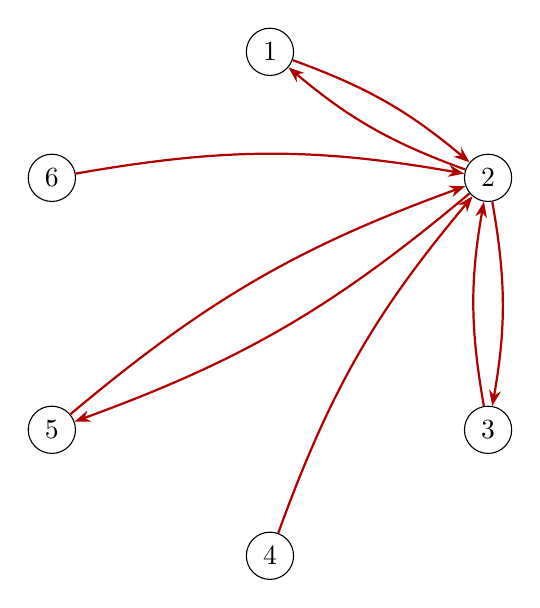
\begin{tikzpicture}[>={Stealth[length=2mm]}]
\node[draw,circle,minimum size=6mm,inner sep=0pt] (n0) at (0.00,3.20) {1};
\node[draw,circle,minimum size=6mm,inner sep=0pt] (n1) at (2.77,1.60) {2};
\node[draw,circle,minimum size=6mm,inner sep=0pt] (n2) at (2.77,-1.60) {3};
\node[draw,circle,minimum size=6mm,inner sep=0pt] (n3) at (0.00,-3.20) {4};
\node[draw,circle,minimum size=6mm,inner sep=0pt] (n4) at (-2.77,-1.60) {5};
\node[draw,circle,minimum size=6mm,inner sep=0pt] (n5) at (-2.77,1.60) {6};
\draw[->,red!70!black,thick] (n0) to[bend left=10] (n1);
\draw[->,red!70!black,thick] (n1) to[bend left=10] (n0);
\draw[->,red!70!black,thick] (n1) to[bend left=10] (n2);
\draw[->,red!70!black,thick] (n1) to[bend left=10] (n4);
\draw[->,red!70!black,thick] (n2) to[bend left=10] (n1);
\draw[->,red!70!black,thick] (n3) to[bend left=10] (n1);
\draw[->,red!70!black,thick] (n4) to[bend left=10] (n1);
\draw[->,red!70!black,thick] (n5) to[bend left=10] (n1);
\end{tikzpicture}
\end{center}
\noindent Solid: defeats. Dashed: supports. Dotted: one party's case is part of another's.
\begin{enumerate}
\item Scriptural reading of Isaiah 7:14, Genesis 3:15 and Micah 5:2–3
\item Critical denial of the predictive reading of Isaiah 7:14
\item Berry’s objection to the near-term exclusion
\item Postell’s parity argument against the near-term exclusion
\item Motyer’s reply to the near-term reading
\item Postell’s Micah counterexample to the near-term exclusion
\end{enumerate}
\begin{longtable}{@{}>{\raggedright\arraybackslash}p{0.3\textwidth} >{\raggedright\arraybackslash}p{0.3\textwidth} >{\raggedright\arraybackslash}p{0.3\textwidth}@{}}
\toprule
\textbf{From} & \textbf{To} & \textbf{Edge} \\
\midrule
\endhead
1 \emph{Scriptural reading of Isaiah 7:14, Genesis 3:15 and Micah 5:2–3} & 2 \emph{Critical denial of the predictive reading of Isaiah 7:14} & defeats \\
2 \emph{Critical denial of the predictive reading of Isaiah 7:14} & 1 \emph{Scriptural reading of Isaiah 7:14, Genesis 3:15 and Micah 5:2–3} & defeats \\
2 \emph{Critical denial of the predictive reading of Isaiah 7:14} & 3 \emph{Berry’s objection to the near-term exclusion} & defeats \\
2 \emph{Critical denial of the predictive reading of Isaiah 7:14} & 5 \emph{Motyer’s reply to the near-term reading} & defeats \\
3 \emph{Berry’s objection to the near-term exclusion} & 2 \emph{Critical denial of the predictive reading of Isaiah 7:14} & defeats \\
4 \emph{Postell’s parity argument against the near-term exclusion} & 2 \emph{Critical denial of the predictive reading of Isaiah 7:14} & defeats \\
5 \emph{Motyer’s reply to the near-term reading} & 2 \emph{Critical denial of the predictive reading of Isaiah 7:14} & defeats \\
6 \emph{Postell’s Micah counterexample to the near-term exclusion} & 2 \emph{Critical denial of the predictive reading of Isaiah 7:14} & defeats \\
\bottomrule
\end{longtable}
\noindent The defeats are the cells of \texttt{isaiah\allowbreak{}Dispute\_\allowbreak{}defeats}, the supports the cells of \texttt{isaiah\allowbreak{}Dispute\_\allowbreak{}supports} and the parts the cells of \texttt{isaiah\allowbreak{}Dispute\_\allowbreak{}part\allowbreak{}Of}, each computed from the parties' premises and checked by the kernel. The attacks derived through support and through parts are reported, not counted: every verdict is computed from the defeats alone. Every derived attack is already a defeat.
\par\medskip\noindent\textbf{\texttt{replies\_\allowbreak{}stand\_\allowbreak{}with\_\allowbreak{}the\_\allowbreak{}scriptural\_\allowbreak{}reading}}\par\nobreak\noindent
\textbf{The scriptural reading and all four replies stand together}, in the world Motyer describes: none of the five defeats another. One fact, settling twenty ordered pairs.

{\small\begin{verbatim}
theorem replies_stand_with_the_scriptural_reading :
    isaiahDispute.StandTogether [Party.scriptural, Party.berry, Party.postell,
    Party.motyer, Party.micah]
-- axioms: propext, Classical.choice, Quot.sound
\end{verbatim}}
\par\medskip\noindent\textbf{\texttt{replies\allowbreak{}Heard\allowbreak{}In\allowbreak{}Stages}}\par\nobreak\noindent
How the scriptural reading prevails, in stages: nothing attacks Postell’s two counterexamples, so they come first; they answer the critic, the only party that attacks the scriptural reading, Berry and Motyer, so those three come next. And the critic does not join them: the scriptural reading attacks it, and nothing among the five answers the scriptural reading.

\paragraph{What the dispute forces is exactly \emph{Postell’s parity argument against the near-term exclusion}, \emph{Postell’s Micah counterexample to the near-term exclusion}, \emph{Scriptural reading of Isaiah 7:14, Genesis 3:15 and Micah 5:2–3}, \emph{Berry’s objection to the near-term exclusion}, \emph{Motyer’s reply to the near-term reading}.}
\begin{itemize}
\item Stage 1: \emph{Postell’s parity argument against the near-term exclusion}, \emph{Postell’s Micah counterexample to the near-term exclusion}.
\begin{itemize}
\item \emph{Postell’s parity argument against the near-term exclusion} is defeated by nothing.
\item \emph{Postell’s Micah counterexample to the near-term exclusion} is defeated by nothing.
\end{itemize}
\item Stage 2: \emph{Scriptural reading of Isaiah 7:14, Genesis 3:15 and Micah 5:2–3}, \emph{Berry’s objection to the near-term exclusion}, \emph{Motyer’s reply to the near-term reading}.
\begin{itemize}
\item \emph{Critical denial of the predictive reading of Isaiah 7:14} defeats \emph{Scriptural reading of Isaiah 7:14, Genesis 3:15 and Micah 5:2–3}, and \emph{Postell’s parity argument against the near-term exclusion} defeats \emph{Critical denial of the predictive reading of Isaiah 7:14}.
\item \emph{Critical denial of the predictive reading of Isaiah 7:14} defeats \emph{Berry’s objection to the near-term exclusion}, and \emph{Postell’s parity argument against the near-term exclusion} defeats \emph{Critical denial of the predictive reading of Isaiah 7:14}.
\item \emph{Critical denial of the predictive reading of Isaiah 7:14} defeats \emph{Motyer’s reply to the near-term reading}, and \emph{Postell’s parity argument against the near-term exclusion} defeats \emph{Critical denial of the predictive reading of Isaiah 7:14}.
\end{itemize}
\item Nothing else is forced:
\begin{itemize}
\item \emph{Scriptural reading of Isaiah 7:14, Genesis 3:15 and Micah 5:2–3} defeats \emph{Critical denial of the predictive reading of Isaiah 7:14}, and nothing forced defeats \emph{Scriptural reading of Isaiah 7:14, Genesis 3:15 and Micah 5:2–3}.
\end{itemize}
\end{itemize}
\par\noindent\textbf{What this rests on.} The reasons state 5 defeats and 27 absences of defeat, each a cell of the defeat table, \texttt{isaiah\allowbreak{}Dispute\_\allowbreak{}defeats}, computed from the two parties' premises and checked by the kernel. Whether an attack survives turns on the attacker's weakest link and on the rating of what it attacks, so a changed rating can change the verdict. The weakest links:
\begin{itemize}
\item \emph{Scriptural reading of Isaiah 7:14, Genesis 3:15 and Micah 5:2–3}, weakest at \emph{disputed}:
\begin{itemize}
\item Isaiah 7:14 is a Messianic prediction of a virgin birth --- \cite[ad loc. Isa 7:14]{motyer-isaiah-1993}; \cite[123]{motyer-context-content-1970}; \cite[12--14]{compton-immanuel-prophecy-2007}; \cite[66]{justin-dialogue-with-trypho-160}; \cite[III.21.6]{irenaeus-against-heresies-180}; \cite[I.35]{origen-against-celsus-248}
\item עַלְמָה in Isaiah 7:14 denotes a virgin, not merely a young woman --- \cite[ad loc. Isa 7:14]{motyer-isaiah-1993}; \cite[app. Isa 7:14]{bhs-1997}; \cite[1653--1654]{berry-virgin-birth-2003}; \cite[125]{motyer-context-content-1970}; \cite[7--8]{compton-immanuel-prophecy-2007}; \cite[I.32]{jerome-against-jovinianus-393}
\item Genesis 3:15 is the protoevangelium, the first promise of a redeemer --- \cite[167]{leupold-exposition-genesis-1942}; \cite[102]{keil-delitzsch-pentateuch-1866}; \cite{miravalle-meet-your-mother-2014}; \cite[318]{lewis-womans-seed-1991}
\item The matrilineal wording of Genesis 3:15 marks a birth with no human father --- \cite[298--299]{luther-on-the-creation-1904}; \cite{miravalle-meet-your-mother-2014}; \cite[ad loc. Gen 3:15]{henry-commentary-whole-bible}
\item Micah’s mention of a mother and no father indicates a birth with no human father --- \cite{miravalle-introduction-mary-2020}
\item An oracle’s meaning in the finished book is set by its literary placement --- \cite[483--486]{postell-isaiah-messianic-2025}
\item Read compositionally, Isaiah 7:14 anticipates a future, miraculous birth --- \cite[490--493]{postell-isaiah-messianic-2025}
\item Mary conceived Jesus while a virgin --- Matt 1:18-25; Luke 1:26-38; \cite[30--33]{brown-problem-virginal-conception-1972}
\item an inference step --- \cite[ad loc. Isa 7:14]{motyer-isaiah-1993}
\item an inference step --- \cite{miravalle-meet-your-mother-2014}
\item an inference step --- \cite{miravalle-introduction-mary-2020}
\item an inference step --- \cite[490--493]{postell-isaiah-messianic-2025}
\item an inference step --- \cite[ad loc. Matt 1:23]{france-matthew-2007}
\end{itemize}
\item \emph{Postell’s parity argument against the near-term exclusion}, weakest at \emph{plausible}:
\begin{itemize}
\item an inference step --- \cite[487--489]{postell-isaiah-messianic-2025}
\end{itemize}
\item \emph{Critical denial of the predictive reading of Isaiah 7:14}, weakest at \emph{disputed}:
\begin{itemize}
\item Isaiah 7:14 is a near-term sign to Ahaz, fulfilled in Isaiah’s generation --- \cite{brown-birth-messiah-1993}
\item A sign given for Ahaz’s generation is not also a prediction of a virgin birth --- \cite{brown-birth-messiah-1993}
\end{itemize}
\item \emph{Berry’s objection to the near-term exclusion}, weakest at \emph{disputed}:
\begin{itemize}
\item an inference step --- \cite[1653--1654]{berry-virgin-birth-2003}; \cite[5]{compton-immanuel-prophecy-2007}
\end{itemize}
\item \emph{Motyer’s reply to the near-term reading}, weakest at \emph{disputed}:
\begin{itemize}
\item an inference step --- \cite[124]{motyer-context-content-1970}; \cite[5]{compton-immanuel-prophecy-2007}
\end{itemize}
\item \emph{Postell’s Micah counterexample to the near-term exclusion}, weakest at \emph{plausible}:
\begin{itemize}
\item an inference step --- \cite[481]{postell-isaiah-messianic-2025}
\end{itemize}
\end{itemize}
\par\medskip\noindent\textbf{\texttt{scriptural\_\allowbreak{}reading\_\allowbreak{}prevails\_\allowbreak{}once\_\allowbreak{}replies\_\allowbreak{}are\_\allowbreak{}heard}}\par\nobreak\noindent
\textbf{Heard out, the scriptural reading prevails.} Nothing defeats either of Postell’s counterexamples, so both are in the grounded extension from the first step. They defeat the critic — the only party that defeats the scriptural reading, Berry or Motyer — so at the second step all three join them; and nothing defends the critic.

{\small\begin{verbatim}
theorem scriptural_reading_prevails_once_replies_are_heard :
    Framework.grounded isaiahDispute.defeats = {Party.scriptural, Party.berry,
    Party.postell, Party.motyer, Party.micah}
-- axioms: propext, Classical.choice, Quot.sound
\end{verbatim}}
\par\medskip\noindent\textbf{\texttt{critic\allowbreak{}Answered\allowbreak{}By\allowbreak{}Postell}}\par\nobreak\noindent
Why the critical denial cannot be defended: Postell attacks it, and nothing answers Postell.

\paragraph{\emph{Critical denial of the predictive reading of Isaiah 7:14} cannot be defended: no admissible position holds it.}
\begin{itemize}
\item \emph{Postell’s parity argument against the near-term exclusion} defeats \emph{Critical denial of the predictive reading of Isaiah 7:14}, and nothing defeats \emph{Postell’s parity argument against the near-term exclusion}.
\end{itemize}
\par\noindent\textbf{What this rests on.} The reasons state 1 defeat and 6 absences of defeat, each a cell of the defeat table, \texttt{isaiah\allowbreak{}Dispute\_\allowbreak{}defeats}, computed from the two parties' premises and checked by the kernel. Whether an attack survives turns on the attacker's weakest link and on the rating of what it attacks, so a changed rating can change the verdict. The weakest links:
\begin{itemize}
\item \emph{Postell’s parity argument against the near-term exclusion}, weakest at \emph{plausible}:
\begin{itemize}
\item an inference step --- \cite[487--489]{postell-isaiah-messianic-2025}
\end{itemize}
\item \emph{Critical denial of the predictive reading of Isaiah 7:14}, weakest at \emph{disputed}:
\begin{itemize}
\item Isaiah 7:14 is a near-term sign to Ahaz, fulfilled in Isaiah’s generation --- \cite{brown-birth-messiah-1993}
\item A sign given for Ahaz’s generation is not also a prediction of a virgin birth --- \cite{brown-birth-messiah-1993}
\end{itemize}
\item \emph{Scriptural reading of Isaiah 7:14, Genesis 3:15 and Micah 5:2–3}, weakest at \emph{disputed}:
\begin{itemize}
\item Isaiah 7:14 is a Messianic prediction of a virgin birth --- \cite[ad loc. Isa 7:14]{motyer-isaiah-1993}; \cite[123]{motyer-context-content-1970}; \cite[12--14]{compton-immanuel-prophecy-2007}; \cite[66]{justin-dialogue-with-trypho-160}; \cite[III.21.6]{irenaeus-against-heresies-180}; \cite[I.35]{origen-against-celsus-248}
\item עַלְמָה in Isaiah 7:14 denotes a virgin, not merely a young woman --- \cite[ad loc. Isa 7:14]{motyer-isaiah-1993}; \cite[app. Isa 7:14]{bhs-1997}; \cite[1653--1654]{berry-virgin-birth-2003}; \cite[125]{motyer-context-content-1970}; \cite[7--8]{compton-immanuel-prophecy-2007}; \cite[I.32]{jerome-against-jovinianus-393}
\item Genesis 3:15 is the protoevangelium, the first promise of a redeemer --- \cite[167]{leupold-exposition-genesis-1942}; \cite[102]{keil-delitzsch-pentateuch-1866}; \cite{miravalle-meet-your-mother-2014}; \cite[318]{lewis-womans-seed-1991}
\item The matrilineal wording of Genesis 3:15 marks a birth with no human father --- \cite[298--299]{luther-on-the-creation-1904}; \cite{miravalle-meet-your-mother-2014}; \cite[ad loc. Gen 3:15]{henry-commentary-whole-bible}
\item Micah’s mention of a mother and no father indicates a birth with no human father --- \cite{miravalle-introduction-mary-2020}
\item An oracle’s meaning in the finished book is set by its literary placement --- \cite[483--486]{postell-isaiah-messianic-2025}
\item Read compositionally, Isaiah 7:14 anticipates a future, miraculous birth --- \cite[490--493]{postell-isaiah-messianic-2025}
\item Mary conceived Jesus while a virgin --- Matt 1:18-25; Luke 1:26-38; \cite[30--33]{brown-problem-virginal-conception-1972}
\item an inference step --- \cite[ad loc. Isa 7:14]{motyer-isaiah-1993}
\item an inference step --- \cite{miravalle-meet-your-mother-2014}
\item an inference step --- \cite{miravalle-introduction-mary-2020}
\item an inference step --- \cite[490--493]{postell-isaiah-messianic-2025}
\item an inference step --- \cite[ad loc. Matt 1:23]{france-matthew-2007}
\end{itemize}
\item \emph{Berry’s objection to the near-term exclusion}, weakest at \emph{disputed}:
\begin{itemize}
\item an inference step --- \cite[1653--1654]{berry-virgin-birth-2003}; \cite[5]{compton-immanuel-prophecy-2007}
\end{itemize}
\item \emph{Motyer’s reply to the near-term reading}, weakest at \emph{disputed}:
\begin{itemize}
\item an inference step --- \cite[124]{motyer-context-content-1970}; \cite[5]{compton-immanuel-prophecy-2007}
\end{itemize}
\item \emph{Postell’s Micah counterexample to the near-term exclusion}, weakest at \emph{plausible}:
\begin{itemize}
\item an inference step --- \cite[481]{postell-isaiah-messianic-2025}
\end{itemize}
\end{itemize}
\par\medskip\noindent\textbf{\texttt{critical\_\allowbreak{}denial\_\allowbreak{}indefensible}}\par\nobreak\noindent
\textbf{The critical denial cannot be defended.} No admissible set contains it: Postell defeats it, and nothing defeats Postell.

{\small\begin{verbatim}
theorem critical_denial_indefensible : ∀ (S : Set Party), Framework.Admissible
    isaiahDispute.defeats S → Party.critical ∉ S
-- axioms: propext, Classical.choice, Quot.sound
\end{verbatim}}
\par\medskip\noindent\textbf{\texttt{scriptural\_\allowbreak{}reading\_\allowbreak{}skeptically\_\allowbreak{}accepted}}\par\nobreak\noindent
So every resolution of the dispute accepts the scriptural reading.

{\small\begin{verbatim}
theorem scriptural_reading_skeptically_accepted :
    Framework.SkepticallyAccepted isaiahDispute.defeats Party.scriptural
-- axioms: propext, Classical.choice, Quot.sound
\end{verbatim}}
\par\medskip\noindent\textbf{\texttt{critical\_\allowbreak{}denial\_\allowbreak{}not\_\allowbreak{}credulously\_\allowbreak{}accepted}}\par\nobreak\noindent
And none accepts the critical denial.

{\small\begin{verbatim}
theorem critical_denial_not_credulously_accepted :
    ¬Framework.CredulouslyAccepted isaiahDispute.defeats Party.critical
-- axioms: propext, Classical.choice, Quot.sound
\end{verbatim}}
\paragraph*{Hearings}
\leavevmode\par\nobreak
The same dispute with some parties not heard. Each hearing is a restriction of \texttt{isaiah\allowbreak{}Dispute}, so its defeats are the ones already proved. In each of these, every party has a defeater, and so nothing prevails.

\par\medskip\noindent\textbf{\texttt{unanswered}}\par\nobreak\noindent
The scriptural reading and the critic alone.

{\small\begin{verbatim}
def unanswered : Dispute Claim { i // i ∈ [Party.scriptural, Party.critical] } :=
  isaiahDispute.restrict fun x =>
    x ∈ [Party.scriptural, Party.critical]
\end{verbatim}}
\par\medskip\noindent\textbf{\texttt{each\allowbreak{}Defeats\allowbreak{}The\allowbreak{}Other}}\par\nobreak\noindent
Why nothing prevails unanswered: the two defeat each other.

\paragraph{Nothing prevails outright: every party is defeated by another.}
\begin{itemize}
\item \emph{Critical denial of the predictive reading of Isaiah 7:14} defeats \emph{Scriptural reading of Isaiah 7:14, Genesis 3:15 and Micah 5:2–3}.
\item \emph{Scriptural reading of Isaiah 7:14, Genesis 3:15 and Micah 5:2–3} defeats \emph{Critical denial of the predictive reading of Isaiah 7:14}.
\end{itemize}
\par\noindent\textbf{What this rests on.} The reasons state 2 defeats and 0 absences of defeat, each a cell of the defeat table, \texttt{isaiah\allowbreak{}Dispute\_\allowbreak{}defeats}, computed from the two parties' premises and checked by the kernel. Whether an attack survives turns on the attacker's weakest link and on the rating of what it attacks, so a changed rating can change the verdict. The weakest links:
\begin{itemize}
\item \emph{Critical denial of the predictive reading of Isaiah 7:14}, weakest at \emph{disputed}:
\begin{itemize}
\item Isaiah 7:14 is a near-term sign to Ahaz, fulfilled in Isaiah’s generation --- \cite{brown-birth-messiah-1993}
\item A sign given for Ahaz’s generation is not also a prediction of a virgin birth --- \cite{brown-birth-messiah-1993}
\end{itemize}
\item \emph{Scriptural reading of Isaiah 7:14, Genesis 3:15 and Micah 5:2–3}, weakest at \emph{disputed}:
\begin{itemize}
\item Isaiah 7:14 is a Messianic prediction of a virgin birth --- \cite[ad loc. Isa 7:14]{motyer-isaiah-1993}; \cite[123]{motyer-context-content-1970}; \cite[12--14]{compton-immanuel-prophecy-2007}; \cite[66]{justin-dialogue-with-trypho-160}; \cite[III.21.6]{irenaeus-against-heresies-180}; \cite[I.35]{origen-against-celsus-248}
\item עַלְמָה in Isaiah 7:14 denotes a virgin, not merely a young woman --- \cite[ad loc. Isa 7:14]{motyer-isaiah-1993}; \cite[app. Isa 7:14]{bhs-1997}; \cite[1653--1654]{berry-virgin-birth-2003}; \cite[125]{motyer-context-content-1970}; \cite[7--8]{compton-immanuel-prophecy-2007}; \cite[I.32]{jerome-against-jovinianus-393}
\item Genesis 3:15 is the protoevangelium, the first promise of a redeemer --- \cite[167]{leupold-exposition-genesis-1942}; \cite[102]{keil-delitzsch-pentateuch-1866}; \cite{miravalle-meet-your-mother-2014}; \cite[318]{lewis-womans-seed-1991}
\item The matrilineal wording of Genesis 3:15 marks a birth with no human father --- \cite[298--299]{luther-on-the-creation-1904}; \cite{miravalle-meet-your-mother-2014}; \cite[ad loc. Gen 3:15]{henry-commentary-whole-bible}
\item Micah’s mention of a mother and no father indicates a birth with no human father --- \cite{miravalle-introduction-mary-2020}
\item An oracle’s meaning in the finished book is set by its literary placement --- \cite[483--486]{postell-isaiah-messianic-2025}
\item Read compositionally, Isaiah 7:14 anticipates a future, miraculous birth --- \cite[490--493]{postell-isaiah-messianic-2025}
\item Mary conceived Jesus while a virgin --- Matt 1:18-25; Luke 1:26-38; \cite[30--33]{brown-problem-virginal-conception-1972}
\item an inference step --- \cite[ad loc. Isa 7:14]{motyer-isaiah-1993}
\item an inference step --- \cite{miravalle-meet-your-mother-2014}
\item an inference step --- \cite{miravalle-introduction-mary-2020}
\item an inference step --- \cite[490--493]{postell-isaiah-messianic-2025}
\item an inference step --- \cite[ad loc. Matt 1:23]{france-matthew-2007}
\end{itemize}
\end{itemize}
\par\medskip\noindent\textbf{\texttt{nothing\_\allowbreak{}prevails\_\allowbreak{}unanswered}}\par\nobreak\noindent
\textbf{Unanswered, nothing prevails.} The scriptural reading and the critical denial defeat each other, so neither is forced, and the grounded extension is empty.

{\small\begin{verbatim}
theorem nothing_prevails_unanswered : Framework.grounded unanswered.defeats =
    ∅
-- axioms: propext, Classical.choice, Quot.sound
\end{verbatim}}
\par\medskip\noindent\textbf{\texttt{motyer\allowbreak{}Alone}}\par\nobreak\noindent
The scriptural reading, the critic, and Motyer.

{\small\begin{verbatim}
def motyerAlone : Dispute Claim { i // i ∈ [Party.scriptural, Party.critical,
    Party.motyer] } :=
  isaiahDispute.restrict fun x =>
    x ∈
      [Party.scriptural, Party.critical,
        Party.motyer]
\end{verbatim}}
\par\medskip\noindent\textbf{\texttt{motyer\allowbreak{}Ties\allowbreak{}With\allowbreak{}The\allowbreak{}Critic}}\par\nobreak\noindent
Why Motyer alone does not settle it: a defeater for each of the three.

\paragraph{Nothing prevails outright: every party is defeated by another.}
\begin{itemize}
\item \emph{Critical denial of the predictive reading of Isaiah 7:14} defeats \emph{Scriptural reading of Isaiah 7:14, Genesis 3:15 and Micah 5:2–3}.
\item \emph{Scriptural reading of Isaiah 7:14, Genesis 3:15 and Micah 5:2–3} defeats \emph{Critical denial of the predictive reading of Isaiah 7:14}.
\item \emph{Critical denial of the predictive reading of Isaiah 7:14} defeats \emph{Motyer’s reply to the near-term reading}.
\end{itemize}
\par\noindent\textbf{What this rests on.} The reasons state 3 defeats and 0 absences of defeat, each a cell of the defeat table, \texttt{isaiah\allowbreak{}Dispute\_\allowbreak{}defeats}, computed from the two parties' premises and checked by the kernel. Whether an attack survives turns on the attacker's weakest link and on the rating of what it attacks, so a changed rating can change the verdict. The weakest links:
\begin{itemize}
\item \emph{Critical denial of the predictive reading of Isaiah 7:14}, weakest at \emph{disputed}:
\begin{itemize}
\item Isaiah 7:14 is a near-term sign to Ahaz, fulfilled in Isaiah’s generation --- \cite{brown-birth-messiah-1993}
\item A sign given for Ahaz’s generation is not also a prediction of a virgin birth --- \cite{brown-birth-messiah-1993}
\end{itemize}
\item \emph{Scriptural reading of Isaiah 7:14, Genesis 3:15 and Micah 5:2–3}, weakest at \emph{disputed}:
\begin{itemize}
\item Isaiah 7:14 is a Messianic prediction of a virgin birth --- \cite[ad loc. Isa 7:14]{motyer-isaiah-1993}; \cite[123]{motyer-context-content-1970}; \cite[12--14]{compton-immanuel-prophecy-2007}; \cite[66]{justin-dialogue-with-trypho-160}; \cite[III.21.6]{irenaeus-against-heresies-180}; \cite[I.35]{origen-against-celsus-248}
\item עַלְמָה in Isaiah 7:14 denotes a virgin, not merely a young woman --- \cite[ad loc. Isa 7:14]{motyer-isaiah-1993}; \cite[app. Isa 7:14]{bhs-1997}; \cite[1653--1654]{berry-virgin-birth-2003}; \cite[125]{motyer-context-content-1970}; \cite[7--8]{compton-immanuel-prophecy-2007}; \cite[I.32]{jerome-against-jovinianus-393}
\item Genesis 3:15 is the protoevangelium, the first promise of a redeemer --- \cite[167]{leupold-exposition-genesis-1942}; \cite[102]{keil-delitzsch-pentateuch-1866}; \cite{miravalle-meet-your-mother-2014}; \cite[318]{lewis-womans-seed-1991}
\item The matrilineal wording of Genesis 3:15 marks a birth with no human father --- \cite[298--299]{luther-on-the-creation-1904}; \cite{miravalle-meet-your-mother-2014}; \cite[ad loc. Gen 3:15]{henry-commentary-whole-bible}
\item Micah’s mention of a mother and no father indicates a birth with no human father --- \cite{miravalle-introduction-mary-2020}
\item An oracle’s meaning in the finished book is set by its literary placement --- \cite[483--486]{postell-isaiah-messianic-2025}
\item Read compositionally, Isaiah 7:14 anticipates a future, miraculous birth --- \cite[490--493]{postell-isaiah-messianic-2025}
\item Mary conceived Jesus while a virgin --- Matt 1:18-25; Luke 1:26-38; \cite[30--33]{brown-problem-virginal-conception-1972}
\item an inference step --- \cite[ad loc. Isa 7:14]{motyer-isaiah-1993}
\item an inference step --- \cite{miravalle-meet-your-mother-2014}
\item an inference step --- \cite{miravalle-introduction-mary-2020}
\item an inference step --- \cite[490--493]{postell-isaiah-messianic-2025}
\item an inference step --- \cite[ad loc. Matt 1:23]{france-matthew-2007}
\end{itemize}
\item \emph{Motyer’s reply to the near-term reading}, weakest at \emph{disputed}:
\begin{itemize}
\item an inference step --- \cite[124]{motyer-context-content-1970}; \cite[5]{compton-immanuel-prophecy-2007}
\end{itemize}
\end{itemize}
\par\medskip\noindent\textbf{\texttt{nothing\_\allowbreak{}prevails\_\allowbreak{}on\_\allowbreak{}motyer\_\allowbreak{}alone}}\par\nobreak\noindent
\textbf{Motyer alone does not settle it.} He and the critic defeat each other, as the scriptural reading and the critic do, so nothing is forced. His inference is contested as the critic’s premises are, and a contested reply cannot carry the verdict alone.

{\small\begin{verbatim}
theorem nothing_prevails_on_motyer_alone : Framework.grounded
    motyerAlone.defeats = ∅
-- axioms: propext, Classical.choice, Quot.sound
\end{verbatim}}
\par\medskip\noindent\textbf{\texttt{without\allowbreak{}Postell}}\par\nobreak\noindent
Every party but Postell’s Isaiah counterexample.

{\small\begin{verbatim}
def withoutPostell : Dispute Claim { i // i ∉ [Party.postell] } :=
  isaiahDispute.restrict fun x =>
    x ∉ [Party.postell]
\end{verbatim}}
\par\medskip\noindent\textbf{\texttt{micah\allowbreak{}Carries\allowbreak{}The\allowbreak{}Verdict}}\par\nobreak\noindent
How the scriptural reading prevails without Postell’s Isaiah argument, in stages: the Micah counterexample first, then the three it defends.

\paragraph{Grounded: \emph{Postell’s Micah counterexample to the near-term exclusion}, \emph{Scriptural reading of Isaiah 7:14, Genesis 3:15 and Micah 5:2–3}, \emph{Berry’s objection to the near-term exclusion}, \emph{Motyer’s reply to the near-term reading}.}
\begin{itemize}
\item Stage 1: \emph{Postell’s Micah counterexample to the near-term exclusion}.
\begin{itemize}
\item \emph{Postell’s Micah counterexample to the near-term exclusion} is defeated by nothing.
\end{itemize}
\item Stage 2: \emph{Scriptural reading of Isaiah 7:14, Genesis 3:15 and Micah 5:2–3}, \emph{Berry’s objection to the near-term exclusion}, \emph{Motyer’s reply to the near-term reading}.
\begin{itemize}
\item \emph{Critical denial of the predictive reading of Isaiah 7:14} defeats \emph{Scriptural reading of Isaiah 7:14, Genesis 3:15 and Micah 5:2–3}, and \emph{Postell’s Micah counterexample to the near-term exclusion} defeats \emph{Critical denial of the predictive reading of Isaiah 7:14}.
\item \emph{Critical denial of the predictive reading of Isaiah 7:14} defeats \emph{Berry’s objection to the near-term exclusion}, and \emph{Postell’s Micah counterexample to the near-term exclusion} defeats \emph{Critical denial of the predictive reading of Isaiah 7:14}.
\item \emph{Critical denial of the predictive reading of Isaiah 7:14} defeats \emph{Motyer’s reply to the near-term reading}, and \emph{Postell’s Micah counterexample to the near-term exclusion} defeats \emph{Critical denial of the predictive reading of Isaiah 7:14}.
\end{itemize}
\end{itemize}
\par\noindent\textbf{What this rests on.} The reasons state 4 defeats and 17 absences of defeat, each a cell of the defeat table, \texttt{isaiah\allowbreak{}Dispute\_\allowbreak{}defeats}, computed from the two parties' premises and checked by the kernel. Whether an attack survives turns on the attacker's weakest link and on the rating of what it attacks, so a changed rating can change the verdict. The weakest links:
\begin{itemize}
\item \emph{Scriptural reading of Isaiah 7:14, Genesis 3:15 and Micah 5:2–3}, weakest at \emph{disputed}:
\begin{itemize}
\item Isaiah 7:14 is a Messianic prediction of a virgin birth --- \cite[ad loc. Isa 7:14]{motyer-isaiah-1993}; \cite[123]{motyer-context-content-1970}; \cite[12--14]{compton-immanuel-prophecy-2007}; \cite[66]{justin-dialogue-with-trypho-160}; \cite[III.21.6]{irenaeus-against-heresies-180}; \cite[I.35]{origen-against-celsus-248}
\item עַלְמָה in Isaiah 7:14 denotes a virgin, not merely a young woman --- \cite[ad loc. Isa 7:14]{motyer-isaiah-1993}; \cite[app. Isa 7:14]{bhs-1997}; \cite[1653--1654]{berry-virgin-birth-2003}; \cite[125]{motyer-context-content-1970}; \cite[7--8]{compton-immanuel-prophecy-2007}; \cite[I.32]{jerome-against-jovinianus-393}
\item Genesis 3:15 is the protoevangelium, the first promise of a redeemer --- \cite[167]{leupold-exposition-genesis-1942}; \cite[102]{keil-delitzsch-pentateuch-1866}; \cite{miravalle-meet-your-mother-2014}; \cite[318]{lewis-womans-seed-1991}
\item The matrilineal wording of Genesis 3:15 marks a birth with no human father --- \cite[298--299]{luther-on-the-creation-1904}; \cite{miravalle-meet-your-mother-2014}; \cite[ad loc. Gen 3:15]{henry-commentary-whole-bible}
\item Micah’s mention of a mother and no father indicates a birth with no human father --- \cite{miravalle-introduction-mary-2020}
\item An oracle’s meaning in the finished book is set by its literary placement --- \cite[483--486]{postell-isaiah-messianic-2025}
\item Read compositionally, Isaiah 7:14 anticipates a future, miraculous birth --- \cite[490--493]{postell-isaiah-messianic-2025}
\item Mary conceived Jesus while a virgin --- Matt 1:18-25; Luke 1:26-38; \cite[30--33]{brown-problem-virginal-conception-1972}
\item an inference step --- \cite[ad loc. Isa 7:14]{motyer-isaiah-1993}
\item an inference step --- \cite{miravalle-meet-your-mother-2014}
\item an inference step --- \cite{miravalle-introduction-mary-2020}
\item an inference step --- \cite[490--493]{postell-isaiah-messianic-2025}
\item an inference step --- \cite[ad loc. Matt 1:23]{france-matthew-2007}
\end{itemize}
\item \emph{Postell’s Micah counterexample to the near-term exclusion}, weakest at \emph{plausible}:
\begin{itemize}
\item an inference step --- \cite[481]{postell-isaiah-messianic-2025}
\end{itemize}
\item \emph{Critical denial of the predictive reading of Isaiah 7:14}, weakest at \emph{disputed}:
\begin{itemize}
\item Isaiah 7:14 is a near-term sign to Ahaz, fulfilled in Isaiah’s generation --- \cite{brown-birth-messiah-1993}
\item A sign given for Ahaz’s generation is not also a prediction of a virgin birth --- \cite{brown-birth-messiah-1993}
\end{itemize}
\item \emph{Berry’s objection to the near-term exclusion}, weakest at \emph{disputed}:
\begin{itemize}
\item an inference step --- \cite[1653--1654]{berry-virgin-birth-2003}; \cite[5]{compton-immanuel-prophecy-2007}
\end{itemize}
\item \emph{Motyer’s reply to the near-term reading}, weakest at \emph{disputed}:
\begin{itemize}
\item an inference step --- \cite[124]{motyer-context-content-1970}; \cite[5]{compton-immanuel-prophecy-2007}
\end{itemize}
\end{itemize}
\par\medskip\noindent\textbf{\texttt{scriptural\_\allowbreak{}reading\_\allowbreak{}prevails\_\allowbreak{}without\_\allowbreak{}postell}}\par\nobreak\noindent
\textbf{Without Postell’s Isaiah argument, the scriptural reading still prevails.} His Micah counterexample is defeated by nothing, and it defends the scriptural reading against the critic, as the Isaiah argument did. An attack on the grounds of either counterexample leaves the verdict standing.

{\small\begin{verbatim}
theorem scriptural_reading_prevails_without_postell : ⟨Party.scriptural, ⋯⟩ ∈
    Framework.grounded withoutPostell.defeats
-- axioms: propext, Classical.choice, Quot.sound
\end{verbatim}}
\par\medskip\noindent\textbf{\texttt{without\allowbreak{}Parity}}\par\nobreak\noindent
Every party but the two counterexamples.

{\small\begin{verbatim}
def withoutParity : Dispute Claim { i // i ∉ [Party.postell, Party.micah] } :=
  isaiahDispute.restrict fun x =>
    x ∉ [Party.postell, Party.micah]
\end{verbatim}}
\par\medskip\noindent\textbf{\texttt{every\allowbreak{}Reply\allowbreak{}Ties\allowbreak{}With\allowbreak{}The\allowbreak{}Critic}}\par\nobreak\noindent
Why nothing prevails without the counterexamples: the critic defeats every reply it faces, and the replies defeat it.

\paragraph{Nothing prevails outright: every party is defeated by another.}
\begin{itemize}
\item \emph{Critical denial of the predictive reading of Isaiah 7:14} defeats \emph{Scriptural reading of Isaiah 7:14, Genesis 3:15 and Micah 5:2–3}.
\item \emph{Scriptural reading of Isaiah 7:14, Genesis 3:15 and Micah 5:2–3} defeats \emph{Critical denial of the predictive reading of Isaiah 7:14}.
\item \emph{Critical denial of the predictive reading of Isaiah 7:14} defeats \emph{Berry’s objection to the near-term exclusion}.
\item \emph{Critical denial of the predictive reading of Isaiah 7:14} defeats \emph{Motyer’s reply to the near-term reading}.
\end{itemize}
\par\noindent\textbf{What this rests on.} The reasons state 4 defeats and 0 absences of defeat, each a cell of the defeat table, \texttt{isaiah\allowbreak{}Dispute\_\allowbreak{}defeats}, computed from the two parties' premises and checked by the kernel. Whether an attack survives turns on the attacker's weakest link and on the rating of what it attacks, so a changed rating can change the verdict. The weakest links:
\begin{itemize}
\item \emph{Critical denial of the predictive reading of Isaiah 7:14}, weakest at \emph{disputed}:
\begin{itemize}
\item Isaiah 7:14 is a near-term sign to Ahaz, fulfilled in Isaiah’s generation --- \cite{brown-birth-messiah-1993}
\item A sign given for Ahaz’s generation is not also a prediction of a virgin birth --- \cite{brown-birth-messiah-1993}
\end{itemize}
\item \emph{Scriptural reading of Isaiah 7:14, Genesis 3:15 and Micah 5:2–3}, weakest at \emph{disputed}:
\begin{itemize}
\item Isaiah 7:14 is a Messianic prediction of a virgin birth --- \cite[ad loc. Isa 7:14]{motyer-isaiah-1993}; \cite[123]{motyer-context-content-1970}; \cite[12--14]{compton-immanuel-prophecy-2007}; \cite[66]{justin-dialogue-with-trypho-160}; \cite[III.21.6]{irenaeus-against-heresies-180}; \cite[I.35]{origen-against-celsus-248}
\item עַלְמָה in Isaiah 7:14 denotes a virgin, not merely a young woman --- \cite[ad loc. Isa 7:14]{motyer-isaiah-1993}; \cite[app. Isa 7:14]{bhs-1997}; \cite[1653--1654]{berry-virgin-birth-2003}; \cite[125]{motyer-context-content-1970}; \cite[7--8]{compton-immanuel-prophecy-2007}; \cite[I.32]{jerome-against-jovinianus-393}
\item Genesis 3:15 is the protoevangelium, the first promise of a redeemer --- \cite[167]{leupold-exposition-genesis-1942}; \cite[102]{keil-delitzsch-pentateuch-1866}; \cite{miravalle-meet-your-mother-2014}; \cite[318]{lewis-womans-seed-1991}
\item The matrilineal wording of Genesis 3:15 marks a birth with no human father --- \cite[298--299]{luther-on-the-creation-1904}; \cite{miravalle-meet-your-mother-2014}; \cite[ad loc. Gen 3:15]{henry-commentary-whole-bible}
\item Micah’s mention of a mother and no father indicates a birth with no human father --- \cite{miravalle-introduction-mary-2020}
\item An oracle’s meaning in the finished book is set by its literary placement --- \cite[483--486]{postell-isaiah-messianic-2025}
\item Read compositionally, Isaiah 7:14 anticipates a future, miraculous birth --- \cite[490--493]{postell-isaiah-messianic-2025}
\item Mary conceived Jesus while a virgin --- Matt 1:18-25; Luke 1:26-38; \cite[30--33]{brown-problem-virginal-conception-1972}
\item an inference step --- \cite[ad loc. Isa 7:14]{motyer-isaiah-1993}
\item an inference step --- \cite{miravalle-meet-your-mother-2014}
\item an inference step --- \cite{miravalle-introduction-mary-2020}
\item an inference step --- \cite[490--493]{postell-isaiah-messianic-2025}
\item an inference step --- \cite[ad loc. Matt 1:23]{france-matthew-2007}
\end{itemize}
\item \emph{Berry’s objection to the near-term exclusion}, weakest at \emph{disputed}:
\begin{itemize}
\item an inference step --- \cite[1653--1654]{berry-virgin-birth-2003}; \cite[5]{compton-immanuel-prophecy-2007}
\end{itemize}
\item \emph{Motyer’s reply to the near-term reading}, weakest at \emph{disputed}:
\begin{itemize}
\item an inference step --- \cite[124]{motyer-context-content-1970}; \cite[5]{compton-immanuel-prophecy-2007}
\end{itemize}
\end{itemize}
\par\medskip\noindent\textbf{\texttt{nothing\_\allowbreak{}prevails\_\allowbreak{}without\_\allowbreak{}the\_\allowbreak{}counterexamples}}\par\nobreak\noindent
\textbf{Without the counterexamples, nothing prevails.} Berry and Motyer each tie with the critic, as the scriptural reading does, so every party is defeated by someone. The verdict rests on the one kind of reply the critic cannot answer — an oracle on the Assyrian timeline, read messianically — and so on the rating of that inference.

{\small\begin{verbatim}
theorem nothing_prevails_without_the_counterexamples : Framework.grounded
    withoutParity.defeats = ∅
-- axioms: propext, Classical.choice, Quot.sound
\end{verbatim}}
\subsection*{Was the woman already pregnant?}
\addcontentsline{toc}{subsection}{Was the woman already pregnant?}
Paul Wegner does not merely say that עַלְמָה means “young woman”. He makes an argument from Isaiah’s grammar. The word translated “shall conceive”, הָרָה, is an adjective, “pregnant”, and it stands as the predicate of the clause: it says what the woman \emph{is}. So the clause reads “the עַלְמָה \emph{is} pregnant”, already, when the sign is given. A pregnant woman is not a virgin, and since this is the one clear case in Isaiah, it settles what the word means there. The argument is encoded at full strength first, with every premise it needs granted, and it is valid (\texttt{wegner\_\allowbreak{}establishes}), because a rival worth answering has to be stated at its strongest.

\subsubsection*{Where its weight rests}
The grammar is not the weak point, and the encoding grants it throughout. Rydelnik, cited here through Postell, who reports him, reads the same predicate adjective and draws the opposite conclusion: the virgin \emph{is} pregnant, and the sign is therefore as deep as Sheol. What the grammar does not supply is that the pregnancy is an \emph{ordinary} one, and that is the premise that rules out a virgin. Take it away and the objection stops (\texttt{wegner\_\allowbreak{}needs\_\allowbreak{}ordinary\_\allowbreak{}pregnancy}).

Wegner’s own case supplies it from the near-term reading of the sign: a sign for Ahaz’s day, which foretells no virgin birth, was an ordinary pregnancy (\texttt{reading\allowbreak{}Supplies\allowbreak{}Ordinary\allowbreak{}Pregnancy}). The conclusion about the word is then turned back against the predictive reading, as the critical case turns it. So the two legs close into a circle. The pregnancy is ordinary because Isaiah foretells no virgin birth, and Isaiah foretells none because the word does not mean a virgin. Postell names it: “because Wegner rejects the messianic interpretation on grammatical-historical grounds, he assumes that עַלְמָה cannot mean ‘virgin’ in Isaiah 7:14” (468 n. 22).

Keep every datum no one disputes, and \emph{neither} end of the circle is settled. Wegner’s conclusion about the word is not established, and it is not refuted either (\texttt{circle\_\allowbreak{}leaves\_\allowbreak{}the\_\allowbreak{}lexical\_\allowbreak{}conclusion\_\allowbreak{}open}, \texttt{circle\_\allowbreak{}leaves\_\allowbreak{}the\_\allowbreak{}denial\_\allowbreak{}open}). A circle of claims can be held all true or all false with nothing to choose between them, so nothing enters the loop and nothing comes out of it, in either direction. That is a demonstration, not a complaint, and it is conditional in the usual way. A defender of Wegner should deny that the ordinary pregnancy comes from the near-term reading this way, and argue that the near-term reading stands on the historical evidence alone.

Postell’s second reply is independent of the first and survives that defence. The other clear עַלְמָה passages Wegner himself lists are cases of virgins, so a single referent cannot be what settles the word’s sense: the same principle would settle it the other way (\texttt{usage\_\allowbreak{}parity\_\allowbreak{}blocks\_\allowbreak{}wegner}). That premise is rated \texttt{plausible}, not \texttt{well\allowbreak{}Supported}, because Postell’s “in fact virgins” is stronger than Wegner’s own discussion of Song of Songs 6:8.

\subsubsection*{The fathers’ sign argument}
The oldest reply goes to the ordinary pregnancy itself. Justin, Irenaeus and Origen answer the near-term reading with one argument. The oracle promised a \emph{sign}, one offered “in the depth or in the height” (7:11), and an ordinary conception happens to every woman who is not barren, so it would be no sign. Rydelnik makes the same move today (\texttt{sign\allowbreak{}Line}). It denies the one ground of Wegner’s objection that the grammar does not supply. What that buys is measured exactly: with the fathers’ grounds in place of the ordinary pregnancy, Wegner’s conclusion about the word is left open by what remains (\texttt{sign\_\allowbreak{}leaves\_\allowbreak{}the\_\allowbreak{}lexical\_\allowbreak{}conclusion\_\allowbreak{}open}). The objection is blocked, and nothing is shown about the word.

The rival is written first, and Wegner holds it himself: a sign need not be a miracle. Isaiah’s own children are “signs and portents” (8:18), and this sign is dated by a child’s infancy (7:16), so its point may be its timing. Rhodea argues the same. The reply blocks the fathers in turn, without supplying Wegner’s ordinary pregnancy (\texttt{reply\_\allowbreak{}leaves\_\allowbreak{}the\_\allowbreak{}pregnancy\_\allowbreak{}open}).

The chapter goes on to weigh the three: Wegner, the fathers and the reply.

\subsubsection*{Who prevails over Wegner’s objection}
The sign argument attacks Wegner’s objection, not the critical denial of the predictive reading, so it belongs to a dispute of its own rather than to \texttt{isaiah\allowbreak{}Dispute}. Three positions meet here: Wegner’s objection at full strength, the fathers’ sign argument against its ordinary pregnancy, and the near-term reply that a sign need not be a miracle.

As in \texttt{Dispute.lean}, who defeats whom is proved, not stipulated:

\begin{itemize}
  \item \textbf{The sign argument defeats Wegner.} It entails the negation of his premise that the pregnancy is an ordinary one, cited \texttt{disputed}.
  \item \textbf{Wegner defeats the sign argument back.} He holds that premise, and so concludes the opposite of the fathers; and each side’s weakest link is \texttt{disputed}.
  \item \textbf{The reply defeats the sign argument}, by entailing the negation of its premise that the sign must be extraordinary, also cited \texttt{disputed}.
  \item \textbf{The sign argument defeats the reply back}, for the same reason Wegner defeats it: it holds the premise the reply denies, and the reply’s inference is \texttt{disputed}.
  \item \textbf{Wegner and the reply do not attack each other.} They stand together in Wegner’s own world, and Wegner is cited for both.
\end{itemize}
\subsubsection*{What follows}
\textbf{Nothing prevails.} Every party is defeated by someone, so no party must be accepted however the disagreements are settled (\texttt{nothing\_\allowbreak{}prevails\_\allowbreak{}over\_\allowbreak{}wegner}). The tie can be broken two ways, and each is proved to be a position that defends itself against every attack on it: the fathers alone (\texttt{sign\_\allowbreak{}is\_\allowbreak{}one\_\allowbreak{}resolution}), or Wegner with the near-term reply (\texttt{wegner\_\allowbreak{}is\_\allowbreak{}the\_\allowbreak{}other\_\allowbreak{}resolution}). Each side is defensible and neither is forced. Hear only Wegner and the fathers and it is the same (\texttt{nothing\_\allowbreak{}prevails\_\allowbreak{}without\_\allowbreak{}the\_\allowbreak{}reply}): the reply is not what holds the fathers back. Wegner’s rebuttal is, because the fathers’ weakest link is no stronger than his.

\subsubsection*{What the ratings decide}
Every party’s weakest link is \texttt{disputed}, so every attack succeeds and the dispute ties. Two ratings would break the tie, and they break it in opposite directions.

\textbf{The fathers’ ground, \texttt{sign\allowbreak{}Must\allowbreak{}Be\allowbreak{}Extraordinary}.} It is \texttt{disputed} because Wegner and Rhodea contest it. Rated \texttt{plausible}, it would make the sign argument stronger than both rivals, since its other ground is \texttt{consensus} and its inference \texttt{plausible}. Wegner’s rebuttal and the reply’s undermining would then both fail. Nothing would defeat the fathers, and the fathers would defeat Wegner outright.

\textbf{The reply’s inference.} It is \texttt{disputed} because Rydelnik grants both of its grounds and denies what it concludes (\texttt{reply\_\allowbreak{}rests\_\allowbreak{}on\_\allowbreak{}its\_\allowbreak{}inference}). Rated \texttt{plausible}, it would make the reply stronger than the fathers, whose rebuttal would then fail. The reply would stand unanswered, and it would defend Wegner against the only party that defeats him.

So the question this dispute cannot settle is the one the sources divide on: whether the sign of 7:14 must be the kind of sign offered at 7:11. Neither the age of the fathers’ argument nor its modern restatement changes that rating, for the reason the chapter “Was Isaiah’s sign only for Ahaz?” gives: an older witness does not make a contested claim uncontested.

\subsubsection*{How this is checked}
\paragraph*{How the results are checked}
\leavevmode\par\nobreak
Every result is tagged \texttt{@[headline]} and followed by \texttt{\#print axioms}, as in the chapter “Four strands, and what each depends on”, and every countermodel is a named reading.

\paragraph*{Wegner’s objection, and the circle in it}
\leavevmode\par\nobreak
\par\medskip\noindent\textbf{\texttt{wegner\_\allowbreak{}establishes}}\par\nobreak\noindent
\textbf{Wegner’s objection is valid on its own terms.} Grant the predicate-adjective parse, grant that the pregnancy it reports is an ordinary one, and grant that the one clear Isaianic referent settles what the word denotes, and the lexical conclusion follows.

Stated first, and at full strength, because the results below are about where its weight rests and are worth nothing if the argument was weak to begin with.

{\small\begin{verbatim}
theorem wegner_establishes : Establishes wegnerLexical
-- axioms: propext, Quot.sound
\end{verbatim}}
\par\medskip\noindent\textbf{\texttt{rydelnik\allowbreak{}Reading}}\par\nobreak\noindent
Rydelnik’s reading, written down: הָרָה is the predicate adjective Wegner says it is, and what it announces is the miracle rather than an ordinary conception — the virgin is pregnant, a sign as deep as Sheol.

{\small\begin{verbatim}
def rydelnikReading : Valuation Claim :=
  fun a =>
    match a with
    | Claim.pregnancyAtTheSignIsOrdinary => False
    | Claim.isaianicAlmahIsNotAVirgin => False
    | x => True
\end{verbatim}}
\par\medskip\noindent\textbf{\texttt{wegner\_\allowbreak{}needs\_\allowbreak{}ordinary\_\allowbreak{}pregnancy}}\par\nobreak\noindent
\textbf{The grammar is not what carries the objection.} Derive the ordinary pregnancy the way Wegner derives it — from the near-term reading of the sign — rather than granting it, and the argument no longer reaches its conclusion, with the parse itself untouched.

So the load-bearing premise is not \texttt{harah\allowbreak{}Is\allowbreak{}Predicate\allowbreak{}Adjective}, which both sides grant, but the reading of the sign that makes the pregnancy an ordinary one. The next result follows that premise back to where it comes from.

{\small\begin{verbatim}
theorem wegner_needs_ordinary_pregnancy : ¬Establishes
    wegnerWithoutOrdinaryPregnancy
-- axioms: propext, Quot.sound
\end{verbatim}}
\par\medskip\noindent\textbf{\texttt{wegner\allowbreak{}Conclusion\allowbreak{}Granted\allowbreak{}Reading}}\par\nobreak\noindent
Wegner’s own conclusion granted: עַלְמָה does not denote a virgin, and Isaiah 7:14 is not a prediction of a virgin birth. The same two legs of the circle are satisfied on this reading as on the one below — the first because its antecedent fails, the second because its consequent holds — which is what makes the circle silent in \emph{both} directions rather than merely unhelpful in one.

Not a convenience: it is the position Wegner argues for, and the reading had to be found rather than assumed. The all-true valuation that serves the same purpose in \texttt{Sola\allowbreak{}Scriptura} does not work here, because \texttt{wegner\allowbreak{}Circle} carries negated grounds.

{\small\begin{verbatim}
def wegnerConclusionGrantedReading : Valuation Claim :=
  fun a =>
    match a with
    | Claim.almahMeansVirgin => False
    | Claim.isaiahPredictsVirginBirth => False
    | x => True
\end{verbatim}}
\par\medskip\noindent\textbf{\texttt{circle\allowbreak{}Ungrounded\allowbreak{}Reading}}\par\nobreak\noindent
The reading that exhibits the circle: the predictive reading of Isaiah 7:14 stands, עַלְמָה may denote a virgin, and the pregnancy the sign announces is not an ordinary one. Every uncontested datum in Wegner’s case is granted — the parse, the near-term setting, the referent principle — and the two legs of the circle are satisfied because each is an implication whose antecedent fails.

{\small\begin{verbatim}
def circleUngroundedReading : Valuation Claim :=
  fun a =>
    match a with
    | Claim.pregnancyAtTheSignIsOrdinary => False
    | Claim.isaianicAlmahIsNotAVirgin => False
    | x => True
\end{verbatim}}
\par\medskip\noindent\textbf{\texttt{circle\_\allowbreak{}leaves\_\allowbreak{}the\_\allowbreak{}lexical\_\allowbreak{}conclusion\_\allowbreak{}open}}\par\nobreak\noindent
\textbf{The circle, shown rather than alleged.} Put both legs in place — the reading supplying the ordinary pregnancy, and the lexical conclusion turned back against the reading — keep every uncontested datum, and the lexical conclusion does not follow.

\texttt{circle\allowbreak{}Ungrounded\allowbreak{}Reading} is why: a cycle of implications is satisfied outright by a valuation on which every node in it is false, because each leg then has a false antecedent. Nothing enters such a loop from outside, so nothing comes out of it. That is what it means for an argument to be circular rather than sound, and it is checkable rather than merely assertable.

What this does \textbf{not} show is that Wegner is wrong. \texttt{wegner\_\allowbreak{}establishes} records that his argument is valid; what the circle costs is the claim that it is an \emph{independent} route to the lexical conclusion. And the result is conditional on \texttt{reading\allowbreak{}Supplies\allowbreak{}Ordinary\allowbreak{}Pregnancy}, which is Postell’s reading of Wegner’s procedure, not Wegner’s own account of it. He would say the near-term reading rests on the historical setting and stands without the lexical finding — in which case the premise is false and the circle is not there. That premise is where a defender of Wegner should press.

{\small\begin{verbatim}
theorem circle_leaves_the_lexical_conclusion_open : Independent
    wegnerCircle.premises (notP Claim.almahMeansVirgin)
-- axioms: propext, Quot.sound
\end{verbatim}}
\par\medskip\noindent\textbf{\texttt{circle\_\allowbreak{}leaves\_\allowbreak{}the\_\allowbreak{}denial\_\allowbreak{}open}}\par\nobreak\noindent
\textbf{And the other end of it is no better off.} The same premises, asked for the denial of the predictive reading instead of the lexical conclusion, fail in the same way and on the same reading.

Both results are needed to make the point. A circle is not an argument that fails to establish one of its nodes; it is one that establishes neither, having no premise outside itself.

{\small\begin{verbatim}
theorem circle_leaves_the_denial_open : Independent wegnerCircle.premises
    (notP Claim.isaiahPredictsVirginBirth)
-- axioms: propext, Quot.sound
\end{verbatim}}
\par\medskip\noindent\textbf{\texttt{usage\allowbreak{}Parity\allowbreak{}Reading}}\par\nobreak\noindent
Postell’s usage reading, written down: the עַלְמָה of Isaiah 7:14 is granted to be no virgin, and a single referent still does not settle what the word denotes — because the other clear cases would settle it the other way.

{\small\begin{verbatim}
def usageParityReading : Valuation Claim :=
  fun a =>
    match a with
    | Claim.oneReferentSettlesDenotation => False
    | x => True
\end{verbatim}}
\par\medskip\noindent\textbf{\texttt{usage\_\allowbreak{}parity\_\allowbreak{}blocks\_\allowbreak{}wegner}}\par\nobreak\noindent
\textbf{Postell’s second reply, and it is independent of the first.} Concede the parse, concede the ordinary pregnancy, concede that the woman of Isaiah 7:14 is no virgin — and the lexical conclusion still does not follow, because the principle that carries it there would carry the other clear cases the opposite way.

This one survives the defence suggested above. An opponent who shows that the near-term reading stands on its own, and so that there is no circle, has not touched the usage parity: the method is still selective. Between them the two replies leave the objection needing both a non-circular route to the ordinary pregnancy and a reason to privilege this occurrence over Genesis 24:43.

{\small\begin{verbatim}
theorem usage_parity_blocks_wegner : ¬Establishes wegnerUnderUsageParity
-- axioms: propext, Quot.sound
\end{verbatim}}
\par\medskip\noindent\textbf{\texttt{referential\allowbreak{}Sign\allowbreak{}Reading}}\par\nobreak\noindent
The fathers’ sign, with the word left to the lexicon: the pregnancy of 7:14 is no ordinary one, and עַלְמָה still does not denote a virgin. It is the referential reading’s world, in which Mary is an עַלְמָה without the word carrying the sense. Every premise of Wegner’s objection under the sign argument holds in it, and so does his lexical conclusion.

{\small\begin{verbatim}
def referentialSignReading : Valuation Claim :=
  fun a =>
    match a with
    | Claim.almahMeansVirgin => False
    | Claim.pregnancyAtTheSignIsOrdinary => False
    | Claim.isaianicAlmahIsNotAVirgin => False
    | x => True
\end{verbatim}}
\par\medskip\noindent\textbf{\texttt{sign\_\allowbreak{}leaves\_\allowbreak{}the\_\allowbreak{}lexical\_\allowbreak{}conclusion\_\allowbreak{}open}}\par\nobreak\noindent
\textbf{The sign argument blocks Wegner’s objection, and settles nothing about the word.} Keep the parse, the near-term setting and the referent principle, put the fathers’ two grounds where the ordinary pregnancy was, and the lexical conclusion is independent of what is left. On Rydelnik’s reading it fails: the virgin is pregnant, a sign as deep as Sheol. On \texttt{referential\allowbreak{}Sign\allowbreak{}Reading} it holds.

So the argument answers the objection where \texttt{wegner\_\allowbreak{}needs\_\allowbreak{}ordinary\_\allowbreak{}pregnancy} says its weight rests, and does no more. It does not show that עַלְמָה denotes a virgin, because it is not about the word at all.

{\small\begin{verbatim}
theorem sign_leaves_the_lexical_conclusion_open : Independent
    wegnerUnderTheSign.premises (notP Claim.almahMeansVirgin)
-- axioms: propext, Quot.sound
\end{verbatim}}
\par\medskip\noindent\textbf{\texttt{near\allowbreak{}Term\allowbreak{}Sign\allowbreak{}Reading}}\par\nobreak\noindent
The near-term reading of the sign, in Wegner’s world: a sign need not be a miracle, the pregnancy is an ordinary one, עַלְמָה does not denote a virgin, and nor, in the Septuagint’s day, did παρθένος.

{\small\begin{verbatim}
def nearTermSignReading : Valuation Claim :=
  fun a =>
    match a with
    | Claim.maternalSilenceImpliesNoHumanFather => False
    | Claim.magisteriumIsDoctrinallyAuthoritative => False
    | Claim.signMustBeExtraordinary => False
    | Claim.almahMeansVirgin => False
    | Claim.parthenosMeansVirgin => False
    | Claim.lawsUseParthenosAsVirgin => False
    | Claim.dinahIsTheLawsParthenos => False
    | Claim.lxxIsaiahUsesParthenosAsVirgin => False
    | x => True
\end{verbatim}}
\par\medskip\noindent\textbf{\texttt{marvel\allowbreak{}Anyway\allowbreak{}Reading}}\par\nobreak\noindent
A sign that need not be a marvel, and is one all the same: the reader who grants the near-term reply and still holds that the pregnancy of 7:14 is no ordinary one, on other grounds than the sign.

{\small\begin{verbatim}
def marvelAnywayReading : Valuation Claim :=
  fun a =>
    match a with
    | Claim.signMustBeExtraordinary => False
    | Claim.pregnancyAtTheSignIsOrdinary => False
    | x => True
\end{verbatim}}
\par\medskip\noindent\textbf{\texttt{reply\_\allowbreak{}leaves\_\allowbreak{}the\_\allowbreak{}pregnancy\_\allowbreak{}open}}\par\nobreak\noindent
\textbf{The near-term reply blocks the sign argument back, and settles nothing about the pregnancy.} Put the reply’s grounds and step where the fathers’ first ground was, keep the second, and whether the pregnancy is an ordinary one is independent of what is left: it is on \texttt{near\allowbreak{}Term\allowbreak{}Sign\allowbreak{}Reading} and it is not on \texttt{marvel\allowbreak{}Anyway\allowbreak{}Reading}.

This is the reply’s whole reach. It takes away the fathers’ reason for denying the ordinary pregnancy; it does not supply Wegner’s reason for asserting it, which still comes from the near-term reading of the sign.

{\small\begin{verbatim}
theorem reply_leaves_the_pregnancy_open : Independent
    signArgumentUnderReply.premises (notP Claim.pregnancyAtTheSignIsOrdinary)
-- axioms: propext, Quot.sound
\end{verbatim}}
\paragraph*{Satisfiability}
\leavevmode\par\nobreak
As in \texttt{Results.lean}: only a package with a positive \texttt{Establishes} result needs a model named, and the sign argument and the reply are given theirs in \texttt{Dispute.Wegner}, where they are established.

\par\medskip\noindent\textbf{\texttt{wegner\allowbreak{}Own\allowbreak{}Reading}}\par\nobreak\noindent
Wegner’s own world: the one clear Isaianic referent is not a virgin, so the word does not denote virginity.

{\small\begin{verbatim}
def wegnerOwnReading : Valuation Claim :=
  fun a =>
    match a with
    | Claim.almahMeansVirgin => False
    | x => True
\end{verbatim}}
\par\medskip\noindent\textbf{\texttt{wegner\allowbreak{}Lexical\_\allowbreak{}is\_\allowbreak{}satisfiable}}\par\nobreak\noindent
Wegner’s objection has a model.

{\small\begin{verbatim}
theorem wegnerLexical_is_satisfiable : Satisfiable wegnerLexical.premises
-- axioms: propext, Quot.sound
\end{verbatim}}
\paragraph*{The sign argument and the reply as positions}
\leavevmode\par\nobreak
\par\medskip\noindent\textbf{\texttt{sign\allowbreak{}Argument\_\allowbreak{}establishes}}\par\nobreak\noindent
The fathers’ sign argument delivers its conclusion.

{\small\begin{verbatim}
theorem signArgument_establishes : Establishes signArgument
-- axioms: propext, Quot.sound
\end{verbatim}}
\par\medskip\noindent\textbf{\texttt{sign\allowbreak{}Argument\_\allowbreak{}is\_\allowbreak{}satisfiable}}\par\nobreak\noindent
The fathers’ sign argument has a model: Rydelnik’s reading, in which the virgin is pregnant and the sign is as deep as Sheol.

{\small\begin{verbatim}
theorem signArgument_is_satisfiable : Satisfiable signArgument.premises
-- axioms: propext, Quot.sound
\end{verbatim}}
\par\medskip\noindent\textbf{\texttt{ordinary\allowbreak{}Sign\allowbreak{}Reply\_\allowbreak{}establishes}}\par\nobreak\noindent
The near-term reply delivers its conclusion.

{\small\begin{verbatim}
theorem ordinarySignReply_establishes : Establishes ordinarySignReply
-- axioms: propext, Quot.sound
\end{verbatim}}
\par\medskip\noindent\textbf{\texttt{ordinary\allowbreak{}Sign\allowbreak{}Reply\_\allowbreak{}is\_\allowbreak{}satisfiable}}\par\nobreak\noindent
The near-term reply has a model: the near-term reading of the sign.

{\small\begin{verbatim}
theorem ordinarySignReply_is_satisfiable : Satisfiable
    ordinarySignReply.premises
-- axioms: propext, Quot.sound
\end{verbatim}}
\par\medskip\noindent\textbf{\texttt{reply\_\allowbreak{}rests\_\allowbreak{}on\_\allowbreak{}its\_\allowbreak{}inference}}\par\nobreak\noindent
\textbf{The reply rests on its inference, not on its observations.} On Rydelnik’s reading Isaiah’s children are signs, 7:16 dates the deliverance by a child’s infancy, and the sign of 7:14 is extraordinary all the same. The two grounds do not decide the question; the step does, and that is why it is rated \texttt{disputed}.

{\small\begin{verbatim}
theorem reply_rests_on_its_inference : ¬Entails ordinarySignLine.grounds (notP
    Claim.signMustBeExtraordinary)
-- axioms: propext, Quot.sound
\end{verbatim}}
\paragraph*{Strength}
\leavevmode\par\nobreak
\par\medskip\noindent\textbf{\texttt{wegner\allowbreak{}Lexical\_\allowbreak{}strength}}\par\nobreak\noindent
Wegner is no stronger than his contested grounds: the ordinary pregnancy, the near-term setting and the referent principle, each cited \texttt{disputed}.

{\small\begin{verbatim}
theorem wegnerLexical_strength : wegnerLexical.strength = 0
-- axioms: propext
\end{verbatim}}
\par\medskip\noindent\textbf{\texttt{sign\allowbreak{}Argument\_\allowbreak{}strength}}\par\nobreak\noindent
The fathers’ second ground is \texttt{consensus} and their inference \texttt{plausible}, but their first ground is \texttt{disputed}, and they are no stronger than it.

{\small\begin{verbatim}
theorem signArgument_strength : signArgument.strength = 0
-- axioms: propext
\end{verbatim}}
\par\medskip\noindent\textbf{\texttt{ordinary\allowbreak{}Sign\allowbreak{}Reply\_\allowbreak{}strength}}\par\nobreak\noindent
The reply’s grounds are \texttt{consensus}, but its inference is \texttt{disputed}.

{\small\begin{verbatim}
theorem ordinarySignReply_strength : ordinarySignReply.strength = 0
-- axioms: propext
\end{verbatim}}
\paragraph*{The defeats}
\leavevmode\par\nobreak
\par\medskip\noindent\textbf{\texttt{sign\_\allowbreak{}defeats\_\allowbreak{}wegner}}\par\nobreak\noindent
\textbf{The sign argument defeats Wegner.} It entails the negation of his premise that the pregnancy is an ordinary one, which, cited \texttt{disputed}, does not outrank it.

{\small\begin{verbatim}
theorem sign_defeats_wegner : Defeats signArgument wegnerLexical
-- axioms: propext, Classical.choice, Quot.sound
\end{verbatim}}
\par\medskip\noindent\textbf{\texttt{wegner\_\allowbreak{}defeats\_\allowbreak{}sign}}\par\nobreak\noindent
\textbf{Wegner defeats the sign argument back.} He holds the premise it denies, so he rebuts it, and it is no stronger than he is.

{\small\begin{verbatim}
theorem wegner_defeats_sign : Defeats wegnerLexical signArgument
-- axioms: propext, Classical.choice, Quot.sound
\end{verbatim}}
\par\medskip\noindent\textbf{\texttt{reply\_\allowbreak{}defeats\_\allowbreak{}sign}}\par\nobreak\noindent
\textbf{The reply defeats the sign argument.} It entails the negation of the fathers’ premise that the sign must be extraordinary, cited \texttt{disputed}.

{\small\begin{verbatim}
theorem reply_defeats_sign : Defeats ordinarySignReply signArgument
-- axioms: propext, Classical.choice, Quot.sound
\end{verbatim}}
\par\medskip\noindent\textbf{\texttt{sign\_\allowbreak{}defeats\_\allowbreak{}reply}}\par\nobreak\noindent
\textbf{The sign argument defeats the reply back.} It holds the premise the reply denies, and the reply’s inference is contested as that premise is.

{\small\begin{verbatim}
theorem sign_defeats_reply : Defeats signArgument ordinarySignReply
-- axioms: propext, Classical.choice, Quot.sound
\end{verbatim}}
\paragraph*{The dispute}
\leavevmode\par\nobreak
\par\medskip\noindent\textbf{\texttt{wegner\allowbreak{}Party\allowbreak{}Node}}\par\nobreak\noindent
The package each party argues from.

{\small\begin{verbatim}
def wegnerPartyNode : WegnerParty → ArgumentPackage Claim :=
  fun x =>
    match x with
    | WegnerParty.wegner => wegnerLexical
    | WegnerParty.sign => signArgument
    | WegnerParty.reply => ordinarySignReply
\end{verbatim}}
\par\medskip\noindent\textbf{\texttt{wegner\allowbreak{}Dispute}}\par\nobreak\noindent
The dispute over Wegner’s objection: every party’s premises have a model, every party establishes its conclusion, and every party’s inferences are rated. Every party’s weakest link ranks at the bottom.

{\small\begin{verbatim}
def wegnerDispute : Dispute Claim WegnerParty :=
  { node := wegnerPartyNode,
    consistent := wegnerDispute._proof_1,
    sound := wegnerDispute._proof_2,
    rated := wegnerDispute._proof_6 }
\end{verbatim}}
\par\medskip\noindent\textbf{\texttt{wegner\allowbreak{}Dispute\_\allowbreak{}defeats}}\par\nobreak\noindent
\textbf{Who defeats whom}, all nine pairs: the fathers and Wegner defeat each other, the fathers and the reply defeat each other, and nothing else. Every cell is computed from the parties’ premises by \texttt{Horn.defeats?} and checked by the kernel.

{\small\begin{verbatim}
theorem wegnerDispute_defeats : ∀ (i j : WegnerParty), wegnerDispute.defeats i
    j ↔ (i, j) ∈ [(WegnerParty.sign, WegnerParty.wegner), (WegnerParty.wegner,
    WegnerParty.sign), (WegnerParty.reply, WegnerParty.sign),
    (WegnerParty.sign, WegnerParty.reply)]
-- axioms: propext, Classical.choice, Quot.sound
\end{verbatim}}
\par\medskip\noindent\textbf{\texttt{wegner\allowbreak{}Dispute\_\allowbreak{}supports}}\par\nobreak\noindent
\textbf{Nothing supports anything} among Wegner, the fathers and the reply, in all nine pairs. Every cell is computed by \texttt{supports?} and checked by the kernel.

{\small\begin{verbatim}
theorem wegnerDispute_supports : ∀ (i j : WegnerParty),
    ¬wegnerDispute.supports i j
-- axioms: propext, Classical.choice, Quot.sound
\end{verbatim}}
\par\medskip\noindent\textbf{\texttt{wegner\allowbreak{}Dispute\_\allowbreak{}part\allowbreak{}Of}}\par\nobreak\noindent
\textbf{No case is part of another’s} here, in all nine pairs, except each party’s own. Every cell is computed by \texttt{part\allowbreak{}Of?} and checked by the kernel.

{\small\begin{verbatim}
theorem wegnerDispute_partOf : ∀ (i j : WegnerParty), wegnerDispute.partOf i j
    ↔ i = j ∨ (i, j) ∈ []
-- axioms: propext, Classical.choice, Quot.sound
\end{verbatim}}
\par\medskip\noindent\textbf{\texttt{wegner\allowbreak{}Map}}\par\nobreak\noindent
The dispute drawn: who defeats whom.

\begin{center}
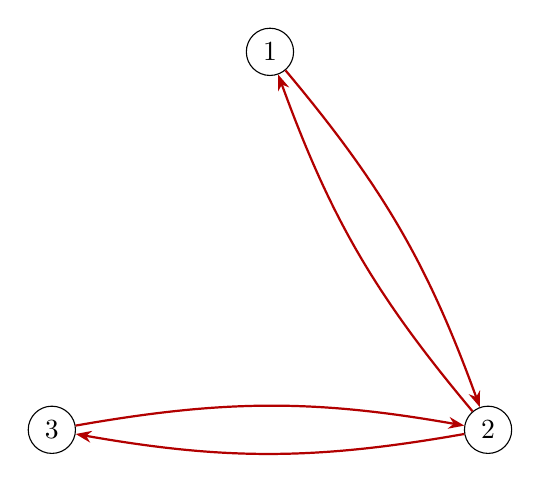
\begin{tikzpicture}[>={Stealth[length=2mm]}]
\node[draw,circle,minimum size=6mm,inner sep=0pt] (n0) at (0.00,3.20) {1};
\node[draw,circle,minimum size=6mm,inner sep=0pt] (n1) at (2.77,-1.60) {2};
\node[draw,circle,minimum size=6mm,inner sep=0pt] (n2) at (-2.77,-1.60) {3};
\draw[->,red!70!black,thick] (n0) to[bend left=10] (n1);
\draw[->,red!70!black,thick] (n1) to[bend left=10] (n0);
\draw[->,red!70!black,thick] (n1) to[bend left=10] (n2);
\draw[->,red!70!black,thick] (n2) to[bend left=10] (n1);
\end{tikzpicture}
\end{center}
\noindent Solid: defeats. Dashed: supports. Dotted: one party's case is part of another's.
\begin{enumerate}
\item Wegner’s grammatical objection: the עַלְמָה is already pregnant
\item The fathers’ sign argument (Isaiah 7:11, 14)
\item The near-term reply: a sign need not be a miracle
\end{enumerate}
\begin{longtable}{@{}>{\raggedright\arraybackslash}p{0.3\textwidth} >{\raggedright\arraybackslash}p{0.3\textwidth} >{\raggedright\arraybackslash}p{0.3\textwidth}@{}}
\toprule
\textbf{From} & \textbf{To} & \textbf{Edge} \\
\midrule
\endhead
1 \emph{Wegner’s grammatical objection: the עַלְמָה is already pregnant} & 2 \emph{The fathers’ sign argument (Isaiah 7:11, 14)} & defeats \\
2 \emph{The fathers’ sign argument (Isaiah 7:11, 14)} & 1 \emph{Wegner’s grammatical objection: the עַלְמָה is already pregnant} & defeats \\
2 \emph{The fathers’ sign argument (Isaiah 7:11, 14)} & 3 \emph{The near-term reply: a sign need not be a miracle} & defeats \\
3 \emph{The near-term reply: a sign need not be a miracle} & 2 \emph{The fathers’ sign argument (Isaiah 7:11, 14)} & defeats \\
\bottomrule
\end{longtable}
\noindent The defeats are the cells of \texttt{wegner\allowbreak{}Dispute\_\allowbreak{}defeats}, the supports the cells of \texttt{wegner\allowbreak{}Dispute\_\allowbreak{}supports} and the parts the cells of \texttt{wegner\allowbreak{}Dispute\_\allowbreak{}part\allowbreak{}Of}, each computed from the parties' premises and checked by the kernel. The attacks derived through support and through parts are reported, not counted: every verdict is computed from the defeats alone. Every derived attack is already a defeat.
\par\medskip\noindent\textbf{\texttt{wegner\_\allowbreak{}stands\_\allowbreak{}with\_\allowbreak{}the\_\allowbreak{}reply}}\par\nobreak\noindent
\textbf{Wegner and the near-term reply stand together}, in Wegner’s own world: the word does not denote a virgin, and the sign need not be a miracle.

{\small\begin{verbatim}
theorem wegner_stands_with_the_reply : wegnerDispute.StandTogether
    [WegnerParty.wegner, WegnerParty.reply]
-- axioms: propext, Classical.choice, Quot.sound
\end{verbatim}}
\par\medskip\noindent\textbf{\texttt{every\allowbreak{}Wegner\allowbreak{}Party\allowbreak{}Defeated}}\par\nobreak\noindent
Why nothing prevails: a defeater for each party.

\paragraph{Nothing prevails outright: every party is defeated by another.}
\begin{itemize}
\item \emph{The fathers’ sign argument (Isaiah 7:11, 14)} defeats \emph{Wegner’s grammatical objection: the עַלְמָה is already pregnant}.
\item \emph{Wegner’s grammatical objection: the עַלְמָה is already pregnant} defeats \emph{The fathers’ sign argument (Isaiah 7:11, 14)}.
\item \emph{The fathers’ sign argument (Isaiah 7:11, 14)} defeats \emph{The near-term reply: a sign need not be a miracle}.
\end{itemize}
\par\noindent\textbf{What this rests on.} The reasons state 3 defeats and 0 absences of defeat, each a cell of the defeat table, \texttt{wegner\allowbreak{}Dispute\_\allowbreak{}defeats}, computed from the two parties' premises and checked by the kernel. Whether an attack survives turns on the attacker's weakest link and on the rating of what it attacks, so a changed rating can change the verdict. The weakest links:
\begin{itemize}
\item \emph{The fathers’ sign argument (Isaiah 7:11, 14)}, weakest at \emph{disputed}:
\begin{itemize}
\item The sign of Isaiah 7:14 must be extraordinary, like the sign offered at 7:11 --- \cite[I.35]{origen-against-celsus-248}; \cite[84]{justin-dialogue-with-trypho-160}; \cite[III.21.6]{irenaeus-against-heresies-180}; \cite[9]{tertullian-answer-to-the-jews-200}; \cite[VII.1]{eusebius-demonstratio-evangelica-315}; \cite[12.22]{cyril-jerusalem-catechetical-lectures-350}; \cite[5]{chrysostom-homilies-matthew-390}; \cite[ad loc. Isa 7:14]{jerome-commentary-isaiah-410}; \cite[ad loc. Isa 7:14]{cyril-alexandria-commentary-isaiah}; \cite[ad loc. Isa 7:14]{theodoret-commentary-isaiah}; \cite[474]{postell-isaiah-messianic-2025}; Isa 7:10-11
\end{itemize}
\item \emph{Wegner’s grammatical objection: the עַלְמָה is already pregnant}, weakest at \emph{disputed}:
\begin{itemize}
\item Isaiah 7:14 is a near-term sign to Ahaz, fulfilled in Isaiah’s generation --- \cite{brown-birth-messiah-1993}
\item The pregnancy Isaiah 7:14 announces is an ordinary conception --- \cite[476--478]{wegner-virgin-births-2011}; \cite[474]{postell-isaiah-messianic-2025}
\item What the עַלְמָה of Isaiah 7:14 turns out to be settles what the word denotes --- \cite[471--472]{wegner-virgin-births-2011}; \cite[468]{postell-isaiah-messianic-2025}; \cite[152]{rico-gentry-infant-king-2020}
\end{itemize}
\item \emph{The near-term reply: a sign need not be a miracle}, weakest at \emph{disputed}:
\begin{itemize}
\item an inference step --- \cite[64--65]{rhodea-did-matthew-conceive-2013}; \cite[469--470]{wegner-virgin-births-2011}; \cite[474]{postell-isaiah-messianic-2025}
\end{itemize}
\end{itemize}
\par\medskip\noindent\textbf{\texttt{nothing\_\allowbreak{}prevails\_\allowbreak{}over\_\allowbreak{}wegner}}\par\nobreak\noindent
\textbf{Nothing prevails.} Every party is defeated by someone — Wegner and the reply by the fathers, the fathers by both — so nothing is forced, and the grounded extension is empty.

{\small\begin{verbatim}
theorem nothing_prevails_over_wegner : Framework.grounded
    wegnerDispute.defeats = ∅
-- axioms: propext, Classical.choice, Quot.sound
\end{verbatim}}
\par\medskip\noindent\textbf{\texttt{fathers\allowbreak{}Alone}}\par\nobreak\noindent
Why the fathers alone are one resolution.

\paragraph{A maximal defensible position: \emph{The fathers’ sign argument (Isaiah 7:11, 14)}.}
\begin{itemize}
\item \emph{The fathers’ sign argument (Isaiah 7:11, 14)} does not defeat itself, and answers each attack on it:
\begin{itemize}
\item \emph{Wegner’s grammatical objection: the עַלְמָה is already pregnant} defeats \emph{The fathers’ sign argument (Isaiah 7:11, 14)}, and \emph{The fathers’ sign argument (Isaiah 7:11, 14)} defeats \emph{Wegner’s grammatical objection: the עַלְמָה is already pregnant}.
\item \emph{The near-term reply: a sign need not be a miracle} defeats \emph{The fathers’ sign argument (Isaiah 7:11, 14)}, and \emph{The fathers’ sign argument (Isaiah 7:11, 14)} defeats \emph{The near-term reply: a sign need not be a miracle}.
\end{itemize}
\item Nothing can be added to it:
\begin{itemize}
\item \emph{Wegner’s grammatical objection: the עַלְמָה is already pregnant} conflicts with \emph{The fathers’ sign argument (Isaiah 7:11, 14)}: \emph{Wegner’s grammatical objection: the עַלְמָה is already pregnant} defeats \emph{The fathers’ sign argument (Isaiah 7:11, 14)}, and \emph{The fathers’ sign argument (Isaiah 7:11, 14)} defeats \emph{Wegner’s grammatical objection: the עַלְמָה is already pregnant}.
\item \emph{The near-term reply: a sign need not be a miracle} conflicts with \emph{The fathers’ sign argument (Isaiah 7:11, 14)}: \emph{The near-term reply: a sign need not be a miracle} defeats \emph{The fathers’ sign argument (Isaiah 7:11, 14)}, and \emph{The fathers’ sign argument (Isaiah 7:11, 14)} defeats \emph{The near-term reply: a sign need not be a miracle}.
\end{itemize}
\end{itemize}
\par\noindent\textbf{What this rests on.} The reasons state 4 defeats and 1 absence of defeat, each a cell of the defeat table, \texttt{wegner\allowbreak{}Dispute\_\allowbreak{}defeats}, computed from the two parties' premises and checked by the kernel. Whether an attack survives turns on the attacker's weakest link and on the rating of what it attacks, so a changed rating can change the verdict. The weakest links:
\begin{itemize}
\item \emph{The fathers’ sign argument (Isaiah 7:11, 14)}, weakest at \emph{disputed}:
\begin{itemize}
\item The sign of Isaiah 7:14 must be extraordinary, like the sign offered at 7:11 --- \cite[I.35]{origen-against-celsus-248}; \cite[84]{justin-dialogue-with-trypho-160}; \cite[III.21.6]{irenaeus-against-heresies-180}; \cite[9]{tertullian-answer-to-the-jews-200}; \cite[VII.1]{eusebius-demonstratio-evangelica-315}; \cite[12.22]{cyril-jerusalem-catechetical-lectures-350}; \cite[5]{chrysostom-homilies-matthew-390}; \cite[ad loc. Isa 7:14]{jerome-commentary-isaiah-410}; \cite[ad loc. Isa 7:14]{cyril-alexandria-commentary-isaiah}; \cite[ad loc. Isa 7:14]{theodoret-commentary-isaiah}; \cite[474]{postell-isaiah-messianic-2025}; Isa 7:10-11
\end{itemize}
\item \emph{Wegner’s grammatical objection: the עַלְמָה is already pregnant}, weakest at \emph{disputed}:
\begin{itemize}
\item Isaiah 7:14 is a near-term sign to Ahaz, fulfilled in Isaiah’s generation --- \cite{brown-birth-messiah-1993}
\item The pregnancy Isaiah 7:14 announces is an ordinary conception --- \cite[476--478]{wegner-virgin-births-2011}; \cite[474]{postell-isaiah-messianic-2025}
\item What the עַלְמָה of Isaiah 7:14 turns out to be settles what the word denotes --- \cite[471--472]{wegner-virgin-births-2011}; \cite[468]{postell-isaiah-messianic-2025}; \cite[152]{rico-gentry-infant-king-2020}
\end{itemize}
\item \emph{The near-term reply: a sign need not be a miracle}, weakest at \emph{disputed}:
\begin{itemize}
\item an inference step --- \cite[64--65]{rhodea-did-matthew-conceive-2013}; \cite[469--470]{wegner-virgin-births-2011}; \cite[474]{postell-isaiah-messianic-2025}
\end{itemize}
\end{itemize}
\par\medskip\noindent\textbf{\texttt{sign\_\allowbreak{}is\_\allowbreak{}one\_\allowbreak{}resolution}}\par\nobreak\noindent
\textbf{One resolution: the fathers.} The sign argument alone is admissible — it defeats both of its defeaters — and it is in conflict with both of the other parties, so no larger set is.

{\small\begin{verbatim}
theorem sign_is_one_resolution : Framework.Preferred wegnerDispute.defeats
    {WegnerParty.sign}
-- axioms: propext, Classical.choice, Quot.sound
\end{verbatim}}
\par\medskip\noindent\textbf{\texttt{wegner\allowbreak{}With\allowbreak{}The\allowbreak{}Reply}}\par\nobreak\noindent
Why Wegner with the reply is the other resolution.

\paragraph{A maximal defensible position: \emph{Wegner’s grammatical objection: the עַלְמָה is already pregnant}, \emph{The near-term reply: a sign need not be a miracle}.}
\begin{itemize}
\item None of \emph{Wegner’s grammatical objection: the עַלְמָה is already pregnant}, \emph{The near-term reply: a sign need not be a miracle} defeats another, and each attack on them is answered from among them:
\begin{itemize}
\item \emph{The fathers’ sign argument (Isaiah 7:11, 14)} defeats \emph{Wegner’s grammatical objection: the עַלְמָה is already pregnant}, and \emph{Wegner’s grammatical objection: the עַלְמָה is already pregnant} defeats \emph{The fathers’ sign argument (Isaiah 7:11, 14)}.
\item \emph{The fathers’ sign argument (Isaiah 7:11, 14)} defeats \emph{The near-term reply: a sign need not be a miracle}, and \emph{Wegner’s grammatical objection: the עַלְמָה is already pregnant} defeats \emph{The fathers’ sign argument (Isaiah 7:11, 14)}.
\end{itemize}
\item Nothing can be added to it:
\begin{itemize}
\item \emph{The fathers’ sign argument (Isaiah 7:11, 14)} conflicts with \emph{Wegner’s grammatical objection: the עַלְמָה is already pregnant}: \emph{The fathers’ sign argument (Isaiah 7:11, 14)} defeats \emph{Wegner’s grammatical objection: the עַלְמָה is already pregnant}, and \emph{Wegner’s grammatical objection: the עַלְמָה is already pregnant} defeats \emph{The fathers’ sign argument (Isaiah 7:11, 14)}.
\end{itemize}
\end{itemize}
\par\noindent\textbf{What this rests on.} The reasons state 3 defeats and 4 absences of defeat, each a cell of the defeat table, \texttt{wegner\allowbreak{}Dispute\_\allowbreak{}defeats}, computed from the two parties' premises and checked by the kernel. Whether an attack survives turns on the attacker's weakest link and on the rating of what it attacks, so a changed rating can change the verdict. The weakest links:
\begin{itemize}
\item \emph{Wegner’s grammatical objection: the עַלְמָה is already pregnant}, weakest at \emph{disputed}:
\begin{itemize}
\item Isaiah 7:14 is a near-term sign to Ahaz, fulfilled in Isaiah’s generation --- \cite{brown-birth-messiah-1993}
\item The pregnancy Isaiah 7:14 announces is an ordinary conception --- \cite[476--478]{wegner-virgin-births-2011}; \cite[474]{postell-isaiah-messianic-2025}
\item What the עַלְמָה of Isaiah 7:14 turns out to be settles what the word denotes --- \cite[471--472]{wegner-virgin-births-2011}; \cite[468]{postell-isaiah-messianic-2025}; \cite[152]{rico-gentry-infant-king-2020}
\end{itemize}
\item \emph{The near-term reply: a sign need not be a miracle}, weakest at \emph{disputed}:
\begin{itemize}
\item an inference step --- \cite[64--65]{rhodea-did-matthew-conceive-2013}; \cite[469--470]{wegner-virgin-births-2011}; \cite[474]{postell-isaiah-messianic-2025}
\end{itemize}
\item \emph{The fathers’ sign argument (Isaiah 7:11, 14)}, weakest at \emph{disputed}:
\begin{itemize}
\item The sign of Isaiah 7:14 must be extraordinary, like the sign offered at 7:11 --- \cite[I.35]{origen-against-celsus-248}; \cite[84]{justin-dialogue-with-trypho-160}; \cite[III.21.6]{irenaeus-against-heresies-180}; \cite[9]{tertullian-answer-to-the-jews-200}; \cite[VII.1]{eusebius-demonstratio-evangelica-315}; \cite[12.22]{cyril-jerusalem-catechetical-lectures-350}; \cite[5]{chrysostom-homilies-matthew-390}; \cite[ad loc. Isa 7:14]{jerome-commentary-isaiah-410}; \cite[ad loc. Isa 7:14]{cyril-alexandria-commentary-isaiah}; \cite[ad loc. Isa 7:14]{theodoret-commentary-isaiah}; \cite[474]{postell-isaiah-messianic-2025}; Isa 7:10-11
\end{itemize}
\end{itemize}
\par\medskip\noindent\textbf{\texttt{wegner\_\allowbreak{}is\_\allowbreak{}the\_\allowbreak{}other\_\allowbreak{}resolution}}\par\nobreak\noindent
\textbf{The other resolution: Wegner, with the near-term reply.} Neither defeats the other, and between them they answer the fathers, who are the only party to defeat either. The fathers are in conflict with both, so no larger set is admissible.

{\small\begin{verbatim}
theorem wegner_is_the_other_resolution : Framework.Preferred
    wegnerDispute.defeats {WegnerParty.wegner, WegnerParty.reply}
-- axioms: propext, Classical.choice, Quot.sound
\end{verbatim}}
\par\medskip\noindent\textbf{\texttt{sign\_\allowbreak{}not\_\allowbreak{}skeptically\_\allowbreak{}accepted}}\par\nobreak\noindent
So the dispute does not force the fathers’ reading.

{\small\begin{verbatim}
theorem sign_not_skeptically_accepted : ¬Framework.SkepticallyAccepted
    wegnerDispute.defeats WegnerParty.sign
-- axioms: propext, Classical.choice, Quot.sound
\end{verbatim}}
\par\medskip\noindent\textbf{\texttt{wegner\_\allowbreak{}not\_\allowbreak{}skeptically\_\allowbreak{}accepted}}\par\nobreak\noindent
Nor does it force Wegner’s.

{\small\begin{verbatim}
theorem wegner_not_skeptically_accepted : ¬Framework.SkepticallyAccepted
    wegnerDispute.defeats WegnerParty.wegner
-- axioms: propext, Classical.choice, Quot.sound
\end{verbatim}}
\paragraph*{A hearing without the reply}
\leavevmode\par\nobreak
\par\medskip\noindent\textbf{\texttt{sign\allowbreak{}Against\allowbreak{}Wegner}}\par\nobreak\noindent
Wegner and the fathers alone.

{\small\begin{verbatim}
def signAgainstWegner : Dispute Claim { i // i ∈ [WegnerParty.wegner,
    WegnerParty.sign] } :=
  wegnerDispute.restrict fun x =>
    x ∈ [WegnerParty.wegner, WegnerParty.sign]
\end{verbatim}}
\par\medskip\noindent\textbf{\texttt{wegner\allowbreak{}And\allowbreak{}The\allowbreak{}Fathers\allowbreak{}Tie}}\par\nobreak\noindent
Why nothing prevails without the reply: Wegner and the fathers defeat each other.

\paragraph{Nothing prevails outright: every party is defeated by another.}
\begin{itemize}
\item \emph{The fathers’ sign argument (Isaiah 7:11, 14)} defeats \emph{Wegner’s grammatical objection: the עַלְמָה is already pregnant}.
\item \emph{Wegner’s grammatical objection: the עַלְמָה is already pregnant} defeats \emph{The fathers’ sign argument (Isaiah 7:11, 14)}.
\end{itemize}
\par\noindent\textbf{What this rests on.} The reasons state 2 defeats and 0 absences of defeat, each a cell of the defeat table, \texttt{wegner\allowbreak{}Dispute\_\allowbreak{}defeats}, computed from the two parties' premises and checked by the kernel. Whether an attack survives turns on the attacker's weakest link and on the rating of what it attacks, so a changed rating can change the verdict. The weakest links:
\begin{itemize}
\item \emph{The fathers’ sign argument (Isaiah 7:11, 14)}, weakest at \emph{disputed}:
\begin{itemize}
\item The sign of Isaiah 7:14 must be extraordinary, like the sign offered at 7:11 --- \cite[I.35]{origen-against-celsus-248}; \cite[84]{justin-dialogue-with-trypho-160}; \cite[III.21.6]{irenaeus-against-heresies-180}; \cite[9]{tertullian-answer-to-the-jews-200}; \cite[VII.1]{eusebius-demonstratio-evangelica-315}; \cite[12.22]{cyril-jerusalem-catechetical-lectures-350}; \cite[5]{chrysostom-homilies-matthew-390}; \cite[ad loc. Isa 7:14]{jerome-commentary-isaiah-410}; \cite[ad loc. Isa 7:14]{cyril-alexandria-commentary-isaiah}; \cite[ad loc. Isa 7:14]{theodoret-commentary-isaiah}; \cite[474]{postell-isaiah-messianic-2025}; Isa 7:10-11
\end{itemize}
\item \emph{Wegner’s grammatical objection: the עַלְמָה is already pregnant}, weakest at \emph{disputed}:
\begin{itemize}
\item Isaiah 7:14 is a near-term sign to Ahaz, fulfilled in Isaiah’s generation --- \cite{brown-birth-messiah-1993}
\item The pregnancy Isaiah 7:14 announces is an ordinary conception --- \cite[476--478]{wegner-virgin-births-2011}; \cite[474]{postell-isaiah-messianic-2025}
\item What the עַלְמָה of Isaiah 7:14 turns out to be settles what the word denotes --- \cite[471--472]{wegner-virgin-births-2011}; \cite[468]{postell-isaiah-messianic-2025}; \cite[152]{rico-gentry-infant-king-2020}
\end{itemize}
\end{itemize}
\par\medskip\noindent\textbf{\texttt{nothing\_\allowbreak{}prevails\_\allowbreak{}without\_\allowbreak{}the\_\allowbreak{}reply}}\par\nobreak\noindent
\textbf{Without the reply, nothing prevails either.} Wegner and the fathers defeat each other, so the reply is not what keeps the fathers from prevailing: Wegner’s rebuttal does, because the fathers’ weakest link is no stronger than his.

{\small\begin{verbatim}
theorem nothing_prevails_without_the_reply : Framework.grounded
    signAgainstWegner.defeats = ∅
-- axioms: propext, Classical.choice, Quot.sound
\end{verbatim}}
\subsection*{What the Septuagint’s word meant}
\addcontentsline{toc}{subsection}{What the Septuagint’s word meant}
The Jews who translated Isaiah into Greek, before Christ, wrote παρθένος, read as “virgin”. That translation, the Septuagint, is the one Matthew quotes. Doesn’t it settle the question?

The argument is old. Irenaeus makes it against Theodotion and Aquila: the verse “was interpreted into Greek by the Jews themselves, much before the period of our Lord’s advent, that there might remain no suspicion that perchance the Jews, complying with our humour, did put this interpretation upon these words” (\emph{Against Heresies} III.21.1). It is encoded here at full strength, and three things are asked of it, one result each.

\textbf{What it rests on.} Take away the claim that παρθένος, in the translator’s Greek, means a virgin, and the Septuagint no longer shows that its translator read the woman as one (\texttt{parthenos\_\allowbreak{}is\_\allowbreak{}load\_\allowbreak{}bearing}). Everything turns on that word, and whether it means “virgin” there is exactly what the sources dispute. Rico and Gentry hold that it does “whenever it appears in Semitic Koine Greek”, and Bratcher agrees. Wegner, Rhodea and Meade hold that in the translator’s day it still meant a young woman, as it does of Dinah after Shechem has lain with her (Genesis 34:3), and Walton that the translator’s choice of it “is not necessarily betraying an interpretation as virgin”. Wegner and Walton grant that by the New Testament the word meant “virgin”; Meade and Davidson put that sense down to Christian use. The dispute is over the translator’s day, two or three centuries before Matthew. The Greek Pentateuch’s laws use the word where virginity is the point, and its law of the seduced παρθένος reads Genesis 34:3 itself otherwise: the woman a man has lain with is still the law’s παρθένος, and owed “the bride-price of virgins” (Exodus 22:15–16). This chapter weighs all five, below, and the Septuagint’s witness prevails, with Rico and Gentry, the laws and that reading of Genesis 34:3; Wegner cannot be defended (\texttt{septuagint\_\allowbreak{}prevails\_\allowbreak{}over\_\allowbreak{}wegner}). The verdict turns on one rating, the status reading’s step, \texttt{plausible} on the readers found.

\textbf{What it would show, if the word means “virgin”.} How one early reader read Isaiah: a Jewish translator, before Christ, read the woman of 7:14 as a virgin, so reading her so is no Christian invention. It would not show what Isaiah’s own word means without a further step, rated \texttt{disputed} (\texttt{septuagint\_\allowbreak{}word\_\allowbreak{}rests\_\allowbreak{}on\_\allowbreak{}its\_\allowbreak{}inference}). A translator can render the woman described rather than the word. The translator of Genesis wrote παρθένος for the עַלְמָה Rebekah (24:43), whom the story has already called a virgin (24:16): a rendering “historically correct — since Rebekah was a virgin”, Bratcher says, that “does not precisely translate the Hebrew” (113). Elsewhere the Septuagint’s translators, of other books than Isaiah, render עַלְמָה with νεᾶνις, “young woman”, four times. That is how this argument’s referential strand already reads the versions.

\textbf{What it leaves open, even then.} The Greek says the virgin \emph{shall} be with child. A woman who is a virgin when the sign is given and conceives later by a man fits those words as well as a virgin who conceives as a virgin does (\texttt{septuagint\_\allowbreak{}leaves\_\allowbreak{}the\_\allowbreak{}conception\_\allowbreak{}open}). That is not only a rival’s reading. Bratcher, who holds that παρθένος “definitely means ‘virgin’ in the LXX” (113), reads the Greek of 7:14 so: “a young woman, at that time virgin, would in the normal way marry and bear a child” (115), “the most reasonable explanation” (116). So the Septuagint, granted every word, does not by itself say that the conception was without a man. Justin and Irenaeus read it so, from the promise of a sign (\texttt{sign\allowbreak{}Line}, weighed in the chapter “Was the woman already pregnant?”); the word alone does not.

\subsubsection*{The word weighed against its rivals}
The Septuagint’s witness rests on one claim, that παρθένος, in its translator’s Greek, means a virgin. Here that claim is weighed against its rival. Six positions meet:

\begin{itemize}
  \item \textbf{The Septuagint as a witness} (Irenaeus): Jews translated Isaiah before Christ and wrote a word that means a virgin, so they read the woman as one.
  \item \textbf{Wegner on παρθένος} (with Rhodea and Meade): in the Septuagint’s day the word meant a young woman of marriageable age, and the sense “virgin” came later. Genesis 34:3 calls Dinah a παρθένος after Shechem has lain with her.
  \item \textbf{Rico and Gentry’s case from usage}: παρθένος means a virgin “whenever it appears in Semitic Koine Greek”, or the Jewish objection to it — Trypho’s, and the Three’s νεᾶνις — would have had no point. The library adds a ground of its own, encoded with theirs: the Greek Isaiah uses the word elsewhere only for בְּתוּלָה.
  \item \textbf{The case from the laws} (Bratcher’s): the Greek Pentateuch, the corpus Genesis 34:3 comes from, uses the word in two laws where virginity is the point. The high priest marries a παρθένος — “a woman in her virginity”, in the Hebrew — and not a widow, a woman put away, a defiled woman or a harlot (Leviticus 21:13–14). A bride without τὰ παρθένια, the tokens of virginity, dies for playing the harlot (Deuteronomy 22:13–21).
  \item \textbf{The status reading of Genesis 34:3}: Wegner’s counterexample read under the law of the seduced παρθένος. The Greek Exodus still calls the woman a man has lain with a παρθένος, and has him pay “the bride-price of virgins” (22:15–16); Genesis 34 tells Shechem’s act in that law’s words. So at 34:3 the word names Dinah by the standing he took from her, in the sense “virgin”.
  \item \textbf{Miller from Genesis 34:3}: “In one passage, this term refers to a rape victim after she has been attacked” (\emph{Born Divine}). The word is said there of a woman no longer a virgin, so it did not by itself connote virginity, and the laws’ virginity is the context’s. His case as the texts leave it: his other example, Joel 1:8, is struck, because the Greek reads otherwise (below, under “a dissent, with what the texts refute struck”).
\end{itemize}
\subsubsection*{What this dispute does not decide}
It is about a Greek word. It is not about the virgin birth, and not about whether Isaiah 7:14 is fulfilled in Christ. That is weighed in \texttt{Dispute}, where the scriptural reading prevails once the replies are heard (\texttt{scriptural\_\allowbreak{}reading\_\allowbreak{}prevails\_\allowbreak{}once\_\allowbreak{}replies\_\allowbreak{}are\_\allowbreak{}heard}) and the critical denial of the prediction belongs to no position that can be defended (\texttt{critical\_\allowbreak{}denial\_\allowbreak{}indefensible}). That shows that the case against the prediction does not survive the replies, on those premises and ratings; it does not prove the prediction. And it needs neither side’s claim about παρθένος.

Nor does it weigh Matthew’s own reading of the word, from his quotation of it of Mary. That is weighed in the chapter “Matthew’s reading of the word”, under each standard.

Nor is it a dispute between believers and unbelievers. Wegner and Rhodea write as evangelicals. Wegner holds that Isaiah 7:14 is used in Matthew “to refer to Mary, who was indeed a virgin”, the “only virgin birth in the Bible” (483). Rhodea turns the weak sense of the word into an argument that Matthew did not invent the virginal conception to fit Isaiah: neither the Hebrew nor the Greek demands it, so Isaiah gave him no reason to (76).

\subsubsection*{What the claims say, and how they are joined}
The claims about the word are claims about its senses. Rico and Gentry’s, encoded, is that “virgin” is a sense of παρθένος in the Septuagint’s Greek; they say more, “whenever it appears”. Wegner’s is that the word meant “young woman” there, and did not yet have the sense “virgin”. Two senses of one word do not exclude each other, so the two claims contradict each other only through Wegner’s “not yet”: the library’s account of what each claim means finds that they cannot both be true (\texttt{Testimony\allowbreak{}Arguments.Meanings.Born\allowbreak{}Of\allowbreak{}AVirgin.joins}).

The laws are joined the same way. The case from the laws concludes that the word has the sense “virgin” in two passages of the Septuagint. A sense a word has in one passage of a text is a sense it has in that text’s usage as a whole (\texttt{Testimony.Ontology.Usage}): a definition of terms, not a reading of any text. So the laws’ sense, if it holds, makes “virgin” one of the word’s senses in the Septuagint’s Greek. That is the claim encoded for Rico and Gentry, and the witness’s ground, and it excludes Wegner’s “not yet ‘virgin’”. It does not say which sense the translator of Isaiah used at 7:14; that move is the witness’s own step. Nor does the definition count a word used \emph{of} a virgin as meaning “virgin”: a thousand uses of “fiancée” of virgins, Walton observes, would not make it mean “virgin” (292). The laws count only because their contexts turn on the sense.

Every party holds these joins, and each attack below is computed with them. In the names of the results, \emph{drift} is Wegner’s case that the word’s sense shifted.

\subsubsection*{How to read the verdicts}
\begin{itemize}
  \item \textbf{Defeats.} One position contradicts another, and the attack survives the ratings. An attack on a premise succeeds unless that premise is rated higher than the attacker’s weakest link. An attack on a conclusion, or on a claim derived on the way, succeeds unless the attacked position is the stronger of the two. A defeat that runs both ways is a \emph{standoff}.
  \item \textbf{Weakest link.} A position is only as strong as its least-supported premise or step. Four parties here rest on something rated \texttt{disputed}, the lowest rating. The status reading rests on a step rated \texttt{plausible}, one above, and so it outranks Wegner.
  \item \textbf{Prevails.} Accepted however every standoff is resolved.
  \item \textbf{A resolution.} A largest set of positions, none of which defeats another, that answers every attack on its members, itself or through an ally. A position in some resolution can be defended; one left out of some resolution is not forced — which is not the same as false.
\end{itemize}
\subsubsection*{What the solver computed}
Six standoffs, three with Wegner and three with Miller; one defeat of each by the status reading, which neither can return; and nothing else (\texttt{septuagint\allowbreak{}Dispute\_\allowbreak{}defeats}, all thirty-six pairs):

\begin{itemize}
  \item \textbf{Wegner and the witness.} What Wegner holds denies the witness’s ground that “virgin” is a sense of the word; what the witness holds denies his conclusion.
  \item \textbf{Wegner and Rico and Gentry.} Each concludes what the other’s conclusion rules out.
  \item \textbf{Wegner and the laws.} The laws’ sense excludes his “not yet ‘virgin’”, and his conclusion excludes theirs.
  \item \textbf{The status reading defeats Wegner.} Its sense “virgin” at Genesis 34:3 excludes his “not yet ‘virgin’”. He attacks it back, by the same exclusion, and the attack fails: he is weaker than it (\texttt{drift\_\allowbreak{}does\_\allowbreak{}not\_\allowbreak{}defeat\_\allowbreak{}dinah}).
  \item \textbf{Miller and the witness, Rico and Gentry, and the laws.} His thesis, that the word did not by itself connote virginity, denies each of their senses, and each of them denies it; his conclusion and the laws’ contradict each other outright.
  \item \textbf{The status reading defeats Miller.} Its sense “virgin” at 34:3 excludes his premise that the noun describes Dinah as she then was, and his thesis. He attacks it back and fails, for the same reason as Wegner. Miller and Wegner do not attack each other: Wegner’s claim entails Miller’s thesis.
\end{itemize}
The witness, Rico and Gentry, the laws and the status reading do not attack one another. They stand together (\texttt{septuagint\_\allowbreak{}stands\_\allowbreak{}with\_\allowbreak{}the\_\allowbreak{}usage}). Rico and Gentry lend the witness its contested ground: their conclusion is that ground, word for word. The laws reach the same ground through the definition, so the library draws no support from them, though they lead to the same place.

\textbf{The Septuagint’s side prevails} (\texttt{septuagint\_\allowbreak{}prevails\_\allowbreak{}over\_\allowbreak{}wegner}). Nothing defeats the status reading, so it is accepted first. It defeats Wegner and Miller, the only parties that defeat the witness, Rico and Gentry or the laws, so all three are accepted with it. Neither Wegner nor Miller belongs to any position that can be defended (\texttt{drift\_\allowbreak{}indefensible}, \texttt{miller\_\allowbreak{}indefensible}). Miller’s defeat overrules his dissent from the laws’ step, so that the step stands at its cited \texttt{well\allowbreak{}Supported} (\texttt{Dispute.Miller}); this dispute weighs the step at \texttt{disputed}, its floor, so the overruling does not lean on the rating it lets stand. That is a verdict on these premises and these ratings, and it turns on one of them, the status reading’s step: see below.

\subsubsection*{Where the evidence lies}
The tie is a tie of ratings, and the ratings count dissenters, not evidence. What each side brings is not alike, and a reader should see it.

For “virgin” as a sense of the word in the Septuagint’s Greek:

\begin{itemize}
  \item \textbf{The Greek Pentateuch’s own usage.} Every בְּתוּלָה and בְּתוּלִים in the Hebrew Pentateuch — fifteen words in fourteen verses — has a παρθεν- word in the Greek, and its laws use the word where virginity is the point (read from Rahlfs’s text and the Masoretic). Across the whole Septuagint, Bratcher counts παρθένος for בְּתוּלָה forty-five times out of fifty-two (113).
  \item \textbf{The lexica on the laws.} LSJ glosses τὰ παρθένια “signs of virginity”, from Deuteronomy 22 (1339); Muraoka, “tokens of virginity” (535); LEH, “signs pertaining to virginity, virginity”. LEH glosses παρθένος itself “virgin” first.
  \item \textbf{Readers who hold the sense, whatever they make of the prophecy.} Rico and Gentry; Bratcher, for whom the word “definitely means ‘virgin’ in the LXX” (113), though he reads 7:14 of a woman then a virgin who conceives “in the normal way” (115); and Delling, for whom the Septuagint’s usage at 7:14 demands “no more than the sense of a ‘woman untouched by a man up to the moment of the conception’” (as Rhodea quotes him, 67 n. 42): a virgin until then, whatever followed. Rhodea, who follows Wegner, still writes that παρθένος “more properly means ‘virgin’” (67), and holds that in the Septuagint it “need not refer to a virgo intacta”.
\end{itemize}
For “young woman, and not yet ‘virgin’”:

\begin{itemize}
  \item \textbf{Early Greek usage.} Early Greek had both senses. LSJ gives “maiden, girl”, “virgin, opp. γυνή”, and “of unmarried women who are not virgins” (1339); BDAG gives the general use “of a young woman of marriageable age, w. or without focus on virginity” from Homer on (777), and the sense “virgin” in the New Testament and the early Christian writings. Every side grants it.
  \item \textbf{Genesis 34:3}, one verse with the word twice, which every side grants: what the Greek reads. How it is read is the status reading’s question.
  \item \textbf{Muraoka’s lexicon}, which glosses παρθένος “young woman”, lists Genesis 34:3, “so called just after having been raped”, and marks “virginity stressed (?)” in the laws of Deuteronomy 22 (535).
  \item \textbf{Readers.} Wegner, Rhodea, Meade, Davidson and Miller; Walton doubts the virgin sense, citing Brown for the word’s broader sense (293 n. 15). Brown himself holds that the translator chose “a deliberate preference for understanding the young woman of Isa 7:14 as a virgin” (\emph{Birth of the Messiah} 148): a claim about how the translator read the woman, not about the word.
\end{itemize}
None of this moves a rating. The solver weighs who contests a claim, not how much evidence each side brings. But it does show what the tie is: between the broader sense of early Greek, with one passage of the Septuagint, read by one side as the rule; and the Septuagint’s usage at large, read by the other as the rule, with that passage the exception.

\subsubsection*{What the ratings decide}
\textbf{The verdict turns on the status reading’s step}, from the law of the seduced παρθένος and the law’s words in Genesis 34 to the sense of the word at 34:3. It is rated \texttt{plausible} (\texttt{dinah\allowbreak{}Line} gives the reasons in full). No cited reader grants its grounds and denies its conclusion. Wegner, Rhodea, Meade, Rico and Gentry and Bratcher read 34:3 as said of a woman no longer a virgin, but none takes up Exodus 22:15–16 or the law’s words in Genesis 34. Frymer-Kensky reads the law and the story together, as the step does, from the Hebrew (80, 91). No reader has been found who makes the status reading of the Greek. It is built here from the texts, and that is why it is rated no higher.

Rated \texttt{disputed}, as it was first encoded, the status reading would stand off with Wegner like the other three, nothing would prevail, and the dispute would have two resolutions: the Septuagint’s side, and Wegner alone. That was computed, before the step’s rating was audited. A reader of the Greek Genesis who has the law before him and still reads 34:3 of a woman no longer a virgin would bring it back. Wevers’s \emph{Notes on the Greek Text of Genesis} and Harl’s \emph{La Genèse} have not been read.

\textbf{Wegner’s step}, from the older usage and Genesis 34:3 to the Septuagint’s sense, is rated \texttt{disputed}, the lowest rating. Rico and Gentry, and Bratcher, grant all its grounds and deny its conclusion: to Rico and Gentry, Genesis 34:3 is “the exception that proves the rule”, an archaism of the Greek Pentateuch (18, 21); to Bratcher, it is “surprising” (113). The higher ratings belong to the grounds, not the step: that early Greek used παρθένος of a young woman (well supported), that the Greek of Genesis 34:3 calls Dinah one (\texttt{consensus}), and that the noun there describes her as she then was (well supported). That last ground is Wegner’s reading of the verse, not the text; every reader on record who takes up the verse holds it, and only the status reading denies it. Neither side’s grounds say what the word meant at Isaiah 7:14.

\textbf{The other three steps}, Rico and Gentry’s from the Jewish objection, the laws’ from what the two laws read, and the witness’s own ground, are each \texttt{disputed}, and the verdict does not need any of them raised.

\begin{itemize}
  \item \textbf{Rico and Gentry’s step.} It is \texttt{disputed} because Davidson (1899) and Meade (2013) grant the objection and read it the other way: the revisers wrote νεᾶνις against a sense Christians had put on the word, not one its translator gave it.
  \item \textbf{The laws’ step} (\texttt{laws\_\allowbreak{}rest\_\allowbreak{}on\_\allowbreak{}their\_\allowbreak{}inference}). It is \texttt{disputed} on one reader. Miller grants that the laws require virgins, and holds that the virginity “has to be inferred from the context”: “parthenos in the Septuagint did not by itself connote what we mean by virginity”. Of what he says of the Greek, the young widow he finds at Joel 1:8 is not there in the Greek, which calls her a bride; the translators did not “consistently” use the word for עַלְמָה; and Genesis 34:3 is what the status reading reads otherwise. His point that the Greek adds “who has not known a man” where virginity matters (Genesis 24:16) translates a clause the Hebrew already has. The rating rests on him all the same. The Joel 1:8 example is struck, because the text refutes it, and his dissent still stands on Genesis 34:3, which the Greek reads as he says (\texttt{Dispute.Miller}).
  \item \textbf{The witness’s own ground}, that “virgin” is a sense of the word, cited \texttt{disputed} because Wegner, Walton, Rhodea and Meade contest it.
\end{itemize}
The dissents on these steps are brief on both sides. Davidson hedges his account of the Three with a “possibly”, though not his account of the word; Meade’s is a blog comment revising his own earlier view. The ratings weigh none of this.

\subsubsection*{A dissent, with what the texts refute struck}
The laws’ step (\texttt{laws\allowbreak{}Line}) is rated \texttt{disputed} on one reader, Robert J. Miller. He grants what the laws of Leviticus 21 and Deuteronomy 22 require, and denies that the word in them means “virgin”: “As in other Greek literature, parthenos in the Septuagint did not by itself connote what we mean by virginity”, so that the virginity “has to be inferred from the context” (\emph{Born Divine}). The question to ask of any such dissent is this: \textbf{does it still stand once the texts it cites are read?}

\subsubsection*{His evidence, read}
Miller gives two uses of the word of a woman who is not a virgin.

\begin{itemize}
  \item \textbf{Joel 1:8}, “Lament like a parthenos dressed in sackcloth for the husband of her youth”, a young widow. The Greek does not read so: it calls the woman νύμφην, a bride, and its παρθεν- word, τὸν παρθενικόν, is of the husband (Rahlfs). The text refutes the claim.
  \item \textbf{Genesis 34:3}: “In one passage, this term refers to a rape victim after she has been attacked.” The Greek calls Dinah a παρθένος in the verse after Shechem lies with her, and that much the text reads. But Miller’s claim is more: that the noun describes her as she then was, no longer a virgin, so that it is not used there in the sense “virgin”. That is his premise, not the text’s. The order of the verses puts Shechem’s love after his act; it does not put the noun’s description there. A noun is read at a time of its own, which the context gives (Enç 1986): Scripture names Rahab “the harlot” long after Jericho (Hebrews 11:31). The status reading takes the noun as the law’s name for the woman a man has lain with (\texttt{dinah\allowbreak{}Line}).
\end{itemize}
\subsubsection*{What the checks find}
The library strikes a claim only when a reading of a text refutes it — Scripture, rated \texttt{consensus} — and then runs every check on what is left (\texttt{Testimony.Logic.Credibility}). Struck of Joel 1:8, Miller’s dissent is his case from Genesis 34:3 (\texttt{miller\_\allowbreak{}struck\_\allowbreak{}is\_\allowbreak{}his\_\allowbreak{}case\_\allowbreak{}from\_\allowbreak{}genesis}), and it still denies the laws’ step, granting the laws’ grounds. His premise about the noun is not struck: no text reads otherwise, and an argument strikes nothing. It is weighed instead.

\begin{itemize}
  \item \textbf{Under the evidence and tradition standards} his dissent is a credible critique. His premise rests on argued scholarship, which both standards admit.
  \item \textbf{Under the Scripture standard} it is not (\texttt{miller\_\allowbreak{}survives\_\allowbreak{}on\_\allowbreak{}genesis}). The laws’ grounds are all Scripture, and a dissent from such a step must rest on Scripture alone. What the Greek of 34:3 reads is Scripture; that its noun describes Dinah as she then was is Miller’s reading of it.
  \item \textbf{His denial needs that premise} (\texttt{miller\_\allowbreak{}rests\_\allowbreak{}on\_\allowbreak{}the\_\allowbreak{}noun}). Grant what the Greek reads and every step of his, and the laws’ sense can still stand.
\end{itemize}
Had Joel 1:8 been all his evidence, the dissent would not count under any standard: struck of it, nothing in it would deny the step (\texttt{miller\_\allowbreak{}on\_\allowbreak{}joel\_\allowbreak{}alone\_\allowbreak{}does\_\allowbreak{}not\_\allowbreak{}count}). That is the rule at work: evidence the texts refute stops counting, and a dissent that needed it stops counting with it.

\subsubsection*{Weighed in the dispute, and overruled}
A credible dissent can still lose when it is weighed. In the dispute above, Miller’s case from Genesis 34:3 is a party, beside Wegner’s, and the solver computes that nothing can defend it (\texttt{miller\_\allowbreak{}indefensible}). The status reading concludes that the word names Dinah in the sense “virgin”, which Miller’s premise and his thesis deny; he attacks it back, and fails, because his step, rated \texttt{disputed}, is weaker than the status reading’s, rated \texttt{plausible}. Nothing answers the status reading, so nothing defends Miller.

A dissent overruled so stops counting against the step (\texttt{Testimony.Logic.Credibility}, \texttt{Overruled}), on one condition, which keeps the rule from arguing in a circle: the dispute must weigh the step at its floor. It does. The case from the laws cites its step \texttt{disputed} there, so Miller is overruled with the laws at their weakest, and the overruling owes nothing to the rating it lets stand.

So the laws’ step stands at its cited \texttt{well\allowbreak{}Supported} under every standard (\texttt{laws\_\allowbreak{}step\_\allowbreak{}ratings}): under the evidence and tradition standards because the one credible dissent is overruled, and under the Scripture standard because it is not heard. The verdict turns, as the dispute’s does, on the status reading’s step, rated \texttt{plausible}. Rated \texttt{disputed}, it would not outrank Miller, he would stand off with it, and his dissent would count again.

\subsubsection*{How this is checked}
\paragraph*{The Septuagint as a witness}
\leavevmode\par\nobreak
Each reading below is a model: a way every claim of the argument could stand at once, named for what it says of the Septuagint and of the woman of 7:14. It settles those as its namesake does. Where the argument’s joins require a side on questions this module does not touch, it takes the scriptural reading’s: that Micah’s mention of a mother and no father does mean something, and that Scripture, not the magisterium, is the judge. Every other claim it leaves true, and none of them bears on the results it is used for.

\par\medskip\noindent\textbf{\texttt{virgin\allowbreak{}Conceives\allowbreak{}Reading}}\par\nobreak\noindent
Justin’s reading of the elders’ Greek, with Rico and Gentry’s sense of the word: παρθένος means a virgin, the translator read the woman of 7:14 as one, and she conceives as one — “a sign which is not common to all the first-born sons” (\emph{Dialogue} 84). So she is not already pregnant when the sign is given, and her pregnancy is no ordinary one. Wegner’s claim is false in it: the word already had the sense “virgin”. So are Miller’s thesis and his premise that the noun of Genesis 34:3 describes Dinah as she then was: the noun names her.

{\small\begin{verbatim}
def virginConceivesReading : Valuation Claim :=
  fun a =>
    match a with
    | Claim.parthenosMeantYoungWoman => False
    | Claim.parthenosDoesNotItselfConnoteVirginity => False
    | Claim.parthenosDescribesDinahAsSheThenWas => False
    | Claim.harahIsPredicateAdjective => False
    | Claim.isaianicAlmahIsAlreadyPregnant => False
    | Claim.pregnancyAtTheSignIsOrdinary => False
    | Claim.isaianicAlmahIsNotAVirgin => False
    | Claim.maternalSilenceProvesNothing => False
    | Claim.magisteriumIsDoctrinallyAuthoritative => False
    | x => True
\end{verbatim}}
\par\medskip\noindent\textbf{\texttt{archaism\allowbreak{}Reading}}\par\nobreak\noindent
Rico and Gentry’s reading of Genesis 34:3: the word there is said of Dinah as she then was, no longer a virgin, an archaism of the Greek Pentateuch, “the exception that proves the rule” (21); and in the Septuagint at large it means a virgin. So the verse uses the word otherwise, and the status reading is false in it; Wegner’s claim is false too. Otherwise as Justin reads the elders’ Greek (\texttt{virgin\allowbreak{}Conceives\allowbreak{}Reading}).

{\small\begin{verbatim}
def archaismReading : Valuation Claim :=
  fun a =>
    match a with
    | Claim.parthenosMeantYoungWoman => False
    | Claim.parthenosDoesNotItselfConnoteVirginity => False
    | Claim.dinahIsTheLawsParthenos => False
    | Claim.harahIsPredicateAdjective => False
    | Claim.isaianicAlmahIsAlreadyPregnant => False
    | Claim.pregnancyAtTheSignIsOrdinary => False
    | Claim.isaianicAlmahIsNotAVirgin => False
    | Claim.maternalSilenceProvesNothing => False
    | Claim.magisteriumIsDoctrinallyAuthoritative => False
    | x => True
\end{verbatim}}
\par\medskip\noindent\textbf{\texttt{septuagint\allowbreak{}Witness\_\allowbreak{}establishes}}\par\nobreak\noindent
\textbf{The Septuagint, read with Rico and Gentry, is a witness from before Christ.} Grant that the Greek Isaiah renders עַלְמָה with παρθένος, that it was made by Jews before Christ, and that παρθένος in its Greek means a virgin, and it follows that a Jewish translator, before Christ, read the woman of 7:14 as a virgin.

That is the whole of what it delivers: a claim about how the first translator read the verse. It does not show that παρθένος meant “virgin” in the translator’s day: that is granted here, and rated \texttt{disputed} (\texttt{parthenos\_\allowbreak{}is\_\allowbreak{}load\_\allowbreak{}bearing}). Nor does it show what עַלְמָה means (\texttt{septuagint\_\allowbreak{}word\_\allowbreak{}rests\_\allowbreak{}on\_\allowbreak{}its\_\allowbreak{}inference}), or how the woman conceived (\texttt{septuagint\_\allowbreak{}leaves\_\allowbreak{}the\_\allowbreak{}conception\_\allowbreak{}open}).

{\small\begin{verbatim}
theorem septuagintWitness_establishes : Establishes septuagintWitness
-- axioms: propext, Quot.sound
\end{verbatim}}
\par\medskip\noindent\textbf{\texttt{septuagint\allowbreak{}Witness\_\allowbreak{}is\_\allowbreak{}satisfiable}}\par\nobreak\noindent
The Septuagint as a witness has a model.

{\small\begin{verbatim}
theorem septuagintWitness_is_satisfiable : Satisfiable
    septuagintWitness.premises
-- axioms: propext, Quot.sound
\end{verbatim}}
\par\medskip\noindent\textbf{\texttt{wegner\allowbreak{}Drift\allowbreak{}Reading}}\par\nobreak\noindent
Wegner’s reading: in the translator’s day παρθένος meant “young woman”, with or without virginity, and did not yet mean “virgin”; so the Greek does not show that its translator read the woman of 7:14 as a virgin, nor anything about how she conceived, and עַלְמָה does not denote a virgin either. The woman of 7:14 is already pregnant when the sign is given, and the sign need not be a miracle. Wegner does not take up the laws of the Greek Pentateuch. This reading extends his view to them as Miller reads them: the laws say what they say, and the word in them still means “young woman”. Nor does he take up Exodus 22:15–16; in this reading Genesis 34 is told in that law’s words, and Dinah is still called a παρθένος in the older sense.

{\small\begin{verbatim}
def wegnerDriftReading : Valuation Claim :=
  fun a =>
    match a with
    | Claim.parthenosMeansVirgin => False
    | Claim.lawsUseParthenosAsVirgin => False
    | Claim.dinahIsTheLawsParthenos => False
    | Claim.lxxIsaiahUsesParthenosAsVirgin => False
    | Claim.lxxReadsAVirgin => False
    | Claim.lxxEnvisagesAVirginalConception => False
    | Claim.almahMeansVirgin => False
    | Claim.signMustBeExtraordinary => False
    | Claim.maternalSilenceProvesNothing => False
    | Claim.magisteriumIsDoctrinallyAuthoritative => False
    | x => True
\end{verbatim}}
\par\medskip\noindent\textbf{\texttt{parthenos\_\allowbreak{}is\_\allowbreak{}load\_\allowbreak{}bearing}}\par\nobreak\noindent
\textbf{The word carries the whole witness.} Keep the rendering and its date — the Greek has παρθένος, and Jews made it before Christ — and grant nothing about what παρθένος meant to them, and the Septuagint no longer shows that its translator read the woman as a virgin. On Wegner’s reading the word was the ordinary one for a young woman of marriageable age.

So whoever argues from the Septuagint has to win the claim about the word. Its date, which the rival grants, does not help without it.

{\small\begin{verbatim}
theorem parthenos_is_load_bearing : ¬Establishes septuagintWithoutTheSense
-- axioms: propext, Quot.sound
\end{verbatim}}
\paragraph*{From the translator’s reading to Isaiah’s word}
\leavevmode\par\nobreak
\par\medskip\noindent\textbf{\texttt{septuagint\allowbreak{}On\allowbreak{}The\allowbreak{}Word\_\allowbreak{}establishes}}\par\nobreak\noindent
Add the step from the translator’s reading to Isaiah’s word, rated \texttt{disputed}, and the case concludes that עַלְמָה denotes a virgin. It is only as good as that step.

{\small\begin{verbatim}
theorem septuagintOnTheWord_establishes : Establishes septuagintOnTheWord
-- axioms: propext, Quot.sound
\end{verbatim}}
\par\medskip\noindent\textbf{\texttt{septuagint\allowbreak{}On\allowbreak{}The\allowbreak{}Word\_\allowbreak{}is\_\allowbreak{}satisfiable}}\par\nobreak\noindent
The Septuagint asked for Isaiah’s word has a model.

{\small\begin{verbatim}
theorem septuagintOnTheWord_is_satisfiable : Satisfiable
    septuagintOnTheWord.premises
-- axioms: propext, Quot.sound
\end{verbatim}}
\par\medskip\noindent\textbf{\texttt{translator\allowbreak{}Describes\allowbreak{}The\allowbreak{}Woman\allowbreak{}Reading}}\par\nobreak\noindent
The referential reading of the Septuagint: its translator read the woman of 7:14 as a virgin, with a word that means one, and עַלְמָה still denotes only a young woman of marriageable age. He described the woman, not the word, and the woman is a virgin.

{\small\begin{verbatim}
def translatorDescribesTheWomanReading : Valuation Claim :=
  fun a =>
    match a with
    | Claim.parthenosMeantYoungWoman => False
    | Claim.parthenosDoesNotItselfConnoteVirginity => False
    | Claim.parthenosDescribesDinahAsSheThenWas => False
    | Claim.almahMeansVirgin => False
    | Claim.harahIsPredicateAdjective => False
    | Claim.isaianicAlmahIsAlreadyPregnant => False
    | Claim.isaianicAlmahIsNotAVirgin => False
    | Claim.maternalSilenceProvesNothing => False
    | Claim.magisteriumIsDoctrinallyAuthoritative => False
    | x => True
\end{verbatim}}
\par\medskip\noindent\textbf{\texttt{septuagint\_\allowbreak{}word\_\allowbreak{}rests\_\allowbreak{}on\_\allowbreak{}its\_\allowbreak{}inference}}\par\nobreak\noindent
\textbf{The Septuagint shows how its translator read the woman, not what Isaiah’s word means.} Grant everything the witness rests on, παρθένος as “virgin” included, and grant that the translator read the woman of 7:14 as a virgin: עַלְמָה can still denote only a young woman, as the referential strand reads it. The step from the one to the other is the weight, and it is rated \texttt{disputed}: Bratcher and Brown grant that the translator read the woman as a virgin and deny that עַלְמָה says so, and Walton holds that the Greek shows “at best ... an interpretational preference rather than a linguistic necessity” (293). On Bratcher’s reading (113), the Septuagint’s translators render the woman, not the word: παρθένος for Rebekah, whom the story calls a virgin (Genesis 24:43), and νεᾶνις at Exodus 2:8, Psalm 67:26 (68:25 in English Bibles), Song 1:3 and 6:8. Jerome reads Rebekah the other way, as showing that עַלְמָה denotes a virgin (\emph{Against Jovinianus} I.32).

So the Septuagint cannot by itself settle the claim that עַלְמָה itself denotes a virgin, however its word is read. If its word means “virgin”, what it can do is what the referential strand already needs: show that a virgin answers the description.

{\small\begin{verbatim}
theorem septuagint_word_rests_on_its_inference : ¬Entails
    septuagintLine.premises (p Claim.almahMeansVirgin)
-- axioms: propext, Quot.sound
\end{verbatim}}
\paragraph*{What the Greek leaves open}
\leavevmode\par\nobreak
\par\medskip\noindent\textbf{\texttt{now\allowbreak{}AVirgin\allowbreak{}Reading}}\par\nobreak\noindent
Bratcher’s reading of the Greek, who holds that its word means a virgin: “a young woman, at that time virgin, would in the normal way marry and bear a child” (115). Rhodea gives the Greek the same reading, granting its sense for argument’s sake and quoting Tsevat: “The pregnancy lies in the future ...; nothing indicates that the woman is also a virgin after the conception” (67). The word means a virgin, the translator read her as one, and she is one when the sign is given; she conceives later, by a man.

{\small\begin{verbatim}
def nowAVirginReading : Valuation Claim :=
  fun a =>
    match a with
    | Claim.parthenosMeantYoungWoman => False
    | Claim.parthenosDoesNotItselfConnoteVirginity => False
    | Claim.parthenosDescribesDinahAsSheThenWas => False
    | Claim.lxxEnvisagesAVirginalConception => False
    | Claim.harahIsPredicateAdjective => False
    | Claim.isaianicAlmahIsAlreadyPregnant => False
    | Claim.isaianicAlmahIsNotAVirgin => False
    | Claim.maternalSilenceProvesNothing => False
    | Claim.magisteriumIsDoctrinallyAuthoritative => False
    | x => True
\end{verbatim}}
\par\medskip\noindent\textbf{\texttt{septuagint\_\allowbreak{}leaves\_\allowbreak{}the\_\allowbreak{}conception\_\allowbreak{}open}}\par\nobreak\noindent
\textbf{Granted every word, the Septuagint leaves the conception open.} Keep the rendering, its date, παρθένος as “virgin”, the reading it delivers, and the tense of the verb — the virgin \emph{shall} be with child — and whether its translator meant a conception without a man is independent of all of it. On Bratcher’s reading, who holds that the word means a virgin, she is a virgin when the sign is given and later conceives in the ordinary way; Rhodea reads it so too, granting the sense for argument’s sake. On Justin’s she conceives as a virgin. Both readings keep every premise.

No premise here speaks to how she conceives, so the result says only that the Greek’s own words leave it open. Justin’s argument that an ordinary conception would be no sign is the sign argument’s, and is weighed in \texttt{Dispute.Wegner}.

The result has two halves: the Greek does not show that the translator meant a conception without a man, and does not show that he did not. If its sense is granted, the Septuagint’s word answers the objection that the virgin reading was a Christian invention; it does not supply the virginal conception. That comes, if it comes, from the promise of a sign (\texttt{sign\allowbreak{}Line}), or from Matthew and Luke.

{\small\begin{verbatim}
theorem septuagint_leaves_the_conception_open : Independent
    septuagintWithTheFuture.premises (p Claim.lxxEnvisagesAVirginalConception)
-- axioms: propext, Quot.sound
\end{verbatim}}
\paragraph*{Wegner and Rico and Gentry as positions}
\leavevmode\par\nobreak
\par\medskip\noindent\textbf{\texttt{drift\allowbreak{}Objection\_\allowbreak{}establishes}}\par\nobreak\noindent
Wegner on παρθένος delivers its conclusion.

{\small\begin{verbatim}
theorem driftObjection_establishes : Establishes driftObjection
-- axioms: propext, Quot.sound
\end{verbatim}}
\par\medskip\noindent\textbf{\texttt{drift\allowbreak{}Objection\_\allowbreak{}is\_\allowbreak{}satisfiable}}\par\nobreak\noindent
Wegner on παρθένος has a model: his own reading, in which the word had not yet come to mean “virgin”.

{\small\begin{verbatim}
theorem driftObjection_is_satisfiable : Satisfiable driftObjection.premises
-- axioms: propext, Quot.sound
\end{verbatim}}
\par\medskip\noindent\textbf{\texttt{drift\_\allowbreak{}rests\_\allowbreak{}on\_\allowbreak{}its\_\allowbreak{}inference}}\par\nobreak\noindent
\textbf{Wegner on παρθένος rests on its inference.} On Rico and Gentry’s reading all three grounds are granted: the older Greek usage, the Greek’s παρθένος at Genesis 34:3, and that the noun there describes Dinah as she then was, no longer a virgin. And the word still means a virgin in the Septuagint at large: the verse is an archaism of the Greek Pentateuch. The grounds do not decide the question; the step does, and that is why it is rated \texttt{disputed}.

{\small\begin{verbatim}
theorem drift_rests_on_its_inference : ¬Entails driftLine.grounds (p
    Claim.parthenosMeantYoungWoman)
-- axioms: propext, Quot.sound
\end{verbatim}}
\par\medskip\noindent\textbf{\texttt{usage\allowbreak{}Case\_\allowbreak{}establishes}}\par\nobreak\noindent
Rico and Gentry’s case delivers its conclusion.

{\small\begin{verbatim}
theorem usageCase_establishes : Establishes usageCase
-- axioms: propext, Quot.sound
\end{verbatim}}
\par\medskip\noindent\textbf{\texttt{usage\allowbreak{}Case\_\allowbreak{}is\_\allowbreak{}satisfiable}}\par\nobreak\noindent
Rico and Gentry’s case has a model: Justin’s reading of the elders’ Greek.

{\small\begin{verbatim}
theorem usageCase_is_satisfiable : Satisfiable usageCase.premises
-- axioms: propext, Quot.sound
\end{verbatim}}
\par\medskip\noindent\textbf{\texttt{usage\_\allowbreak{}rests\_\allowbreak{}on\_\allowbreak{}its\_\allowbreak{}inference}}\par\nobreak\noindent
\textbf{Rico and Gentry’s case rests on its inference.} On the reading Davidson (1899, 456) and Meade (2013) give, Trypho objects to παρθένος and the Three write νεᾶνις because by then Christians had put the sense “virgin” on the word, while in the translator’s day it still meant a young woman; and the Greek Isaiah’s other παρθένοι still render בְּתוּלָה. The countermodel is Wegner’s reading, which allows all of this. The grounds do not decide the question; the step does, and that is why it is rated \texttt{disputed}.

{\small\begin{verbatim}
theorem usage_rests_on_its_inference : ¬Entails usageLine.grounds (p
    Claim.parthenosMeansVirgin)
-- axioms: propext, Quot.sound
\end{verbatim}}
\par\medskip\noindent\textbf{\texttt{laws\allowbreak{}Case\_\allowbreak{}establishes}}\par\nobreak\noindent
The case from the laws delivers its conclusion.

{\small\begin{verbatim}
theorem lawsCase_establishes : Establishes lawsCase
-- axioms: propext, Quot.sound
\end{verbatim}}
\par\medskip\noindent\textbf{\texttt{laws\allowbreak{}Case\_\allowbreak{}is\_\allowbreak{}satisfiable}}\par\nobreak\noindent
The case from the laws has a model: the reading Justin gives the elders’ Greek, extended to the laws. “Virgin” is a sense of the word, and the laws use it so.

{\small\begin{verbatim}
theorem lawsCase_is_satisfiable : Satisfiable lawsCase.premises
-- axioms: propext, Quot.sound
\end{verbatim}}
\par\medskip\noindent\textbf{\texttt{laws\_\allowbreak{}rest\_\allowbreak{}on\_\allowbreak{}their\_\allowbreak{}inference}}\par\nobreak\noindent
\textbf{The case from the laws rests on its inference.} The high priest’s παρθένος is set against the widow and the harlot, and the bride without τὰ παρθένια dies as a harlot; and still, on Miller’s reading, which Wegner’s thesis requires, the word itself means a young woman there, as at Genesis 34:3. What the laws read does not decide the word’s sense; the step does, and its rating is one of the four that would decide the dispute.

{\small\begin{verbatim}
theorem laws_rest_on_their_inference : ¬Entails lawsLine.grounds (p
    Claim.lawsUseParthenosAsVirgin)
-- axioms: propext, Quot.sound
\end{verbatim}}
\par\medskip\noindent\textbf{\texttt{dinah\allowbreak{}Case\_\allowbreak{}establishes}}\par\nobreak\noindent
The status reading delivers its conclusion.

{\small\begin{verbatim}
theorem dinahCase_establishes : Establishes dinahCase
-- axioms: propext, Quot.sound
\end{verbatim}}
\par\medskip\noindent\textbf{\texttt{dinah\allowbreak{}Case\_\allowbreak{}is\_\allowbreak{}satisfiable}}\par\nobreak\noindent
The status reading has a model: the reading Justin gives the elders’ Greek, extended to Genesis 34. “Virgin” is a sense of the word, and Dinah is called by it.

{\small\begin{verbatim}
theorem dinahCase_is_satisfiable : Satisfiable dinahCase.premises
-- axioms: propext, Quot.sound
\end{verbatim}}
\par\medskip\noindent\textbf{\texttt{dinah\_\allowbreak{}rests\_\allowbreak{}on\_\allowbreak{}its\_\allowbreak{}inference}}\par\nobreak\noindent
\textbf{The status reading rests on its inference.} Grant what Exodus 22:15–16 reads, and that Genesis 34 tells Shechem’s act in the words of the laws: on Wegner’s reading, which Rico and Gentry share for this verse, the Greek still calls Dinah a παρθένος in the older sense, “young woman”, and not as the law’s virgin. The texts do not decide which; the step does, and that is why it is rated \texttt{disputed}.

{\small\begin{verbatim}
theorem dinah_rests_on_its_inference : ¬Entails dinahLine.grounds (p
    Claim.dinahIsTheLawsParthenos)
-- axioms: propext, Quot.sound
\end{verbatim}}
\par\medskip\noindent\textbf{\texttt{miller\allowbreak{}Case\_\allowbreak{}establishes}}\par\nobreak\noindent
Miller from Genesis 34:3 delivers his conclusion.

{\small\begin{verbatim}
theorem millerCase_establishes : Establishes millerCase
-- axioms: propext, Quot.sound
\end{verbatim}}
\par\medskip\noindent\textbf{\texttt{miller\allowbreak{}Case\_\allowbreak{}is\_\allowbreak{}satisfiable}}\par\nobreak\noindent
Miller from Genesis 34:3 has a model: Wegner’s reading, which takes the laws as Miller reads them, and the noun at 34:3 as said of Dinah as she then was.

{\small\begin{verbatim}
theorem millerCase_is_satisfiable : Satisfiable millerCase.premises
-- axioms: propext, Quot.sound
\end{verbatim}}
\paragraph*{Strength}
\leavevmode\par\nobreak
\par\medskip\noindent\textbf{\texttt{septuagint\allowbreak{}Witness\_\allowbreak{}strength}}\par\nobreak\noindent
The witness is no stronger than its claim about the word, cited \texttt{disputed}. Its step is rated \texttt{plausible}, and does not lower it further.

{\small\begin{verbatim}
theorem septuagintWitness_strength : septuagintWitness.strength = 0
-- axioms: propext
\end{verbatim}}
\par\medskip\noindent\textbf{\texttt{drift\allowbreak{}Objection\_\allowbreak{}strength}}\par\nobreak\noindent
Wegner’s grounds are well supported and \texttt{consensus}, but his inference is \texttt{disputed}, on Rico and Gentry and on Bratcher.

{\small\begin{verbatim}
theorem driftObjection_strength : driftObjection.strength = 0
-- axioms: propext
\end{verbatim}}
\par\medskip\noindent\textbf{\texttt{usage\allowbreak{}Case\_\allowbreak{}strength}}\par\nobreak\noindent
Rico and Gentry’s grounds are \texttt{consensus}, but their inference is \texttt{disputed}, on Davidson and Meade.

{\small\begin{verbatim}
theorem usageCase_strength : usageCase.strength = 0
-- axioms: propext
\end{verbatim}}
\par\medskip\noindent\textbf{\texttt{miller\allowbreak{}Case\_\allowbreak{}strength}}\par\nobreak\noindent
Miller’s grounds are \texttt{consensus}, what the Greek reads, and \texttt{well\allowbreak{}Supported}, his premise about the noun; but his inference is \texttt{disputed}, on Rico and Gentry and on Bratcher, who grant both and hold the word means “virgin”.

{\small\begin{verbatim}
theorem millerCase_strength : millerCase.strength = 0
-- axioms: propext
\end{verbatim}}
\par\medskip\noindent\textbf{\texttt{laws\allowbreak{}Case\_\allowbreak{}strength}}\par\nobreak\noindent
The laws’ grounds are \texttt{consensus}, what the Greek reads, but their inference is \texttt{disputed}, on Miller.

{\small\begin{verbatim}
theorem lawsCase_strength : lawsCase.strength = 0
-- axioms: propext
\end{verbatim}}
\par\medskip\noindent\textbf{\texttt{dinah\allowbreak{}Case\_\allowbreak{}strength}}\par\nobreak\noindent
The status reading’s grounds are \texttt{consensus}, what the texts read, and its inference is \texttt{plausible}: no cited reader grants the law’s words in Genesis 34 and denies it, and none has been found who argues it.

{\small\begin{verbatim}
theorem dinahCase_strength : dinahCase.strength = 1
-- axioms: propext
\end{verbatim}}
\paragraph*{The defeats}
\leavevmode\par\nobreak
\par\medskip\noindent\textbf{\texttt{drift\_\allowbreak{}defeats\_\allowbreak{}septuagint}}\par\nobreak\noindent
\textbf{Wegner defeats the Septuagint’s witness.} What he holds — his conclusion, with what it means — denies the witness’s ground that παρθένος means a virgin, which, cited \texttt{disputed}, does not outrank him.

{\small\begin{verbatim}
theorem drift_defeats_septuagint : Defeats driftObjection septuagintWitness
-- axioms: propext, Classical.choice, Quot.sound
\end{verbatim}}
\par\medskip\noindent\textbf{\texttt{septuagint\_\allowbreak{}defeats\_\allowbreak{}drift}}\par\nobreak\noindent
\textbf{The witness defeats Wegner back}, so the two stand off. It holds that the word means a virgin, which denies what Wegner concludes, and he is no stronger than it.

{\small\begin{verbatim}
theorem septuagint_defeats_drift : Defeats septuagintWitness driftObjection
-- axioms: propext, Classical.choice, Quot.sound
\end{verbatim}}
\par\medskip\noindent\textbf{\texttt{drift\_\allowbreak{}defeats\_\allowbreak{}usage}}\par\nobreak\noindent
\textbf{Wegner defeats Rico and Gentry.} His conclusion denies theirs.

{\small\begin{verbatim}
theorem drift_defeats_usage : Defeats driftObjection usageCase
-- axioms: propext, Classical.choice, Quot.sound
\end{verbatim}}
\par\medskip\noindent\textbf{\texttt{usage\_\allowbreak{}defeats\_\allowbreak{}drift}}\par\nobreak\noindent
\textbf{Rico and Gentry defeat Wegner.} Their conclusion denies his.

{\small\begin{verbatim}
theorem usage_defeats_drift : Defeats usageCase driftObjection
-- axioms: propext, Classical.choice, Quot.sound
\end{verbatim}}
\par\medskip\noindent\textbf{\texttt{drift\_\allowbreak{}defeats\_\allowbreak{}laws}}\par\nobreak\noindent
\textbf{Wegner defeats the case from the laws.} That the word had not yet come to mean “virgin” excludes that the laws used it in that sense, because a sense the word has in one passage of the Septuagint is a sense of the Septuagint’s Greek. The laws, at \texttt{disputed}, are no stronger than he.

{\small\begin{verbatim}
theorem drift_defeats_laws : Defeats driftObjection lawsCase
-- axioms: propext, Classical.choice, Quot.sound
\end{verbatim}}
\par\medskip\noindent\textbf{\texttt{laws\_\allowbreak{}defeats\_\allowbreak{}drift}}\par\nobreak\noindent
\textbf{The case from the laws defeats Wegner.} Their sense “virgin” excludes his “not yet ‘virgin’”, and he is no stronger than they.

{\small\begin{verbatim}
theorem laws_defeats_drift : Defeats lawsCase driftObjection
-- axioms: propext, Classical.choice, Quot.sound
\end{verbatim}}
\par\medskip\noindent\textbf{\texttt{drift\_\allowbreak{}does\_\allowbreak{}not\_\allowbreak{}defeat\_\allowbreak{}dinah}}\par\nobreak\noindent
\textbf{Wegner does not defeat the status reading.} That the word had not yet come to mean “virgin” excludes that Genesis 34:3 uses it in that sense, by the same definition, so he attacks it. But a rebuttal succeeds only if the attacker is no weaker than the attacked, and Wegner, whose step is \texttt{disputed}, is weaker than the status reading, whose step is \texttt{plausible}.

{\small\begin{verbatim}
theorem drift_does_not_defeat_dinah : ¬Defeats driftObjection dinahCase
-- axioms: propext, Classical.choice, Quot.sound
\end{verbatim}}
\par\medskip\noindent\textbf{\texttt{dinah\_\allowbreak{}defeats\_\allowbreak{}drift}}\par\nobreak\noindent
\textbf{The status reading defeats Wegner.} Its sense “virgin” at Genesis 34:3 excludes his “not yet ‘virgin’”, and he is no stronger than it.

{\small\begin{verbatim}
theorem dinah_defeats_drift : Defeats dinahCase driftObjection
-- axioms: propext, Classical.choice, Quot.sound
\end{verbatim}}
\paragraph*{The dispute}
\leavevmode\par\nobreak
\par\medskip\noindent\textbf{\texttt{septuagint\allowbreak{}Party\allowbreak{}Node}}\par\nobreak\noindent
The package each party argues from.

{\small\begin{verbatim}
def septuagintPartyNode : SeptuagintParty → ArgumentPackage Claim :=
  fun x =>
    match x with
    | SeptuagintParty.witness => septuagintWitness
    | SeptuagintParty.drift => driftObjection
    | SeptuagintParty.usage => usageCase
    | SeptuagintParty.laws => lawsCase
    | SeptuagintParty.dinah => dinahCase
    | SeptuagintParty.miller => millerCase
\end{verbatim}}
\par\medskip\noindent\textbf{\texttt{septuagint\allowbreak{}Dispute}}\par\nobreak\noindent
The dispute over the Septuagint’s word: every party’s premises have a model, every party establishes its conclusion, and every party’s inferences are rated. Each party’s weakest link is at the bottom, but the status reading’s, one step up.

{\small\begin{verbatim}
def septuagintDispute : Dispute Claim SeptuagintParty :=
  { node := septuagintPartyNode,
    consistent := septuagintDispute._proof_1,
    sound := septuagintDispute._proof_2,
    rated := septuagintDispute._proof_9 }
\end{verbatim}}
\par\medskip\noindent\textbf{\texttt{septuagint\allowbreak{}Dispute\_\allowbreak{}defeats}}\par\nobreak\noindent
\textbf{Who defeats whom}, all thirty-six pairs: Wegner defeats the witness, Rico and Gentry and the laws, and each defeats him back; so does Miller, and each defeats him back; the status reading defeats Wegner and Miller, and neither defeats it; and nothing else. Every cell is computed from what the parties hold by \texttt{Horn.defeats?} and checked by the kernel.

{\small\begin{verbatim}
theorem septuagintDispute_defeats : ∀ (i j : SeptuagintParty),
    septuagintDispute.defeats i j ↔ (i, j) ∈ [(SeptuagintParty.drift,
    SeptuagintParty.witness), (SeptuagintParty.witness,
    SeptuagintParty.drift), (SeptuagintParty.drift, SeptuagintParty.usage),
    (SeptuagintParty.usage, SeptuagintParty.drift), (SeptuagintParty.drift,
    SeptuagintParty.laws), (SeptuagintParty.laws, SeptuagintParty.drift),
    (SeptuagintParty.dinah, SeptuagintParty.drift), (SeptuagintParty.miller,
    SeptuagintParty.witness), (SeptuagintParty.witness,
    SeptuagintParty.miller), (SeptuagintParty.miller, SeptuagintParty.usage),
    (SeptuagintParty.usage, SeptuagintParty.miller), (SeptuagintParty.miller,
    SeptuagintParty.laws), (SeptuagintParty.laws, SeptuagintParty.miller),
    (SeptuagintParty.dinah, SeptuagintParty.miller)]
-- axioms: propext, Classical.choice, Quot.sound
\end{verbatim}}
\par\medskip\noindent\textbf{\texttt{septuagint\allowbreak{}Dispute\_\allowbreak{}supports}}\par\nobreak\noindent
\textbf{One support}, in all thirty-six pairs: Rico and Gentry’s conclusion is the witness’s contested ground, that “virgin” is a sense of παρθένος. The library draws a support only where one party’s conclusion is, word for word, another’s premise. The laws and the status reading reach the witness’s ground through a definition, so no support is drawn from them, though they lead to the same ground. Every cell is computed by \texttt{supports?} and checked by the kernel.

{\small\begin{verbatim}
theorem septuagintDispute_supports : ∀ (i j : SeptuagintParty),
    septuagintDispute.supports i j ↔ (i, j) ∈ [(SeptuagintParty.usage,
    SeptuagintParty.witness)]
-- axioms: propext, Classical.choice, Quot.sound
\end{verbatim}}
\par\medskip\noindent\textbf{\texttt{septuagint\allowbreak{}Dispute\_\allowbreak{}part\allowbreak{}Of}}\par\nobreak\noindent
\textbf{No case is part of another’s} here, in all thirty-six pairs, except each party’s own. Every cell is computed by \texttt{part\allowbreak{}Of?} and checked by the kernel.

{\small\begin{verbatim}
theorem septuagintDispute_partOf : ∀ (i j : SeptuagintParty),
    septuagintDispute.partOf i j ↔ i = j ∨ (i, j) ∈ []
-- axioms: propext, Classical.choice, Quot.sound
\end{verbatim}}
\par\medskip\noindent\textbf{\texttt{septuagint\allowbreak{}Map}}\par\nobreak\noindent
The dispute drawn: who defeats whom, and the one support.

\begin{center}
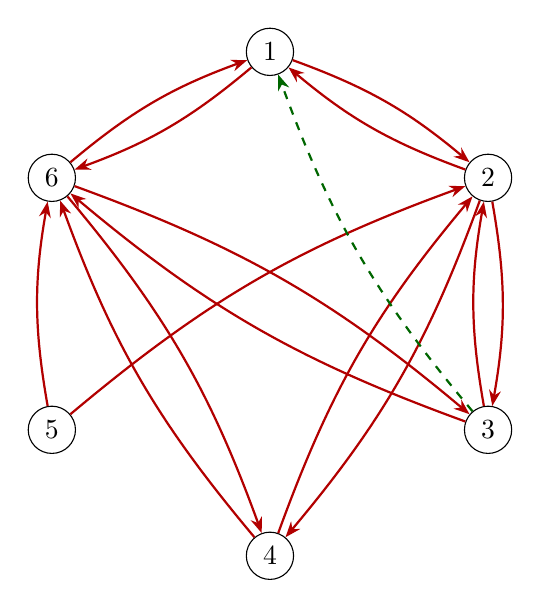
\begin{tikzpicture}[>={Stealth[length=2mm]}]
\node[draw,circle,minimum size=6mm,inner sep=0pt] (n0) at (0.00,3.20) {1};
\node[draw,circle,minimum size=6mm,inner sep=0pt] (n1) at (2.77,1.60) {2};
\node[draw,circle,minimum size=6mm,inner sep=0pt] (n2) at (2.77,-1.60) {3};
\node[draw,circle,minimum size=6mm,inner sep=0pt] (n3) at (0.00,-3.20) {4};
\node[draw,circle,minimum size=6mm,inner sep=0pt] (n4) at (-2.77,-1.60) {5};
\node[draw,circle,minimum size=6mm,inner sep=0pt] (n5) at (-2.77,1.60) {6};
\draw[->,red!70!black,thick] (n0) to[bend left=10] (n1);
\draw[->,red!70!black,thick] (n0) to[bend left=10] (n5);
\draw[->,red!70!black,thick] (n1) to[bend left=10] (n0);
\draw[->,red!70!black,thick] (n1) to[bend left=10] (n2);
\draw[->,red!70!black,thick] (n1) to[bend left=10] (n3);
\draw[->,red!70!black,thick] (n2) to[bend left=10] (n1);
\draw[->,red!70!black,thick] (n2) to[bend left=10] (n5);
\draw[->,red!70!black,thick] (n3) to[bend left=10] (n1);
\draw[->,red!70!black,thick] (n3) to[bend left=10] (n5);
\draw[->,red!70!black,thick] (n4) to[bend left=10] (n1);
\draw[->,red!70!black,thick] (n4) to[bend left=10] (n5);
\draw[->,red!70!black,thick] (n5) to[bend left=10] (n0);
\draw[->,red!70!black,thick] (n5) to[bend left=10] (n2);
\draw[->,red!70!black,thick] (n5) to[bend left=10] (n3);
\draw[->,green!40!black,thick,dashed] (n2) to[bend left=10] (n0);
\end{tikzpicture}
\end{center}
\noindent Solid: defeats. Dashed: supports. Dotted: one party's case is part of another's.
\begin{enumerate}
\item The Septuagint as a witness (Isaiah 7:14 in Greek)
\item Wegner on παρθένος: the word had not yet come to mean ‘virgin’
\item Rico and Gentry: παρθένος means ‘virgin’ in the Greek of the Scriptures
\item The laws of the Greek Pentateuch: παρθένος in the sense ‘virgin’
\item The law’s name for Dinah: Genesis 34:3 read under Exodus 22:15–16
\item Miller, from Genesis 34:3
\end{enumerate}
\begin{longtable}{@{}>{\raggedright\arraybackslash}p{0.3\textwidth} >{\raggedright\arraybackslash}p{0.3\textwidth} >{\raggedright\arraybackslash}p{0.3\textwidth}@{}}
\toprule
\textbf{From} & \textbf{To} & \textbf{Edge} \\
\midrule
\endhead
1 \emph{The Septuagint as a witness (Isaiah 7:14 in Greek)} & 2 \emph{Wegner on παρθένος: the word had not yet come to mean ‘virgin’} & defeats \\
1 \emph{The Septuagint as a witness (Isaiah 7:14 in Greek)} & 6 \emph{Miller, from Genesis 34:3} & defeats \\
2 \emph{Wegner on παρθένος: the word had not yet come to mean ‘virgin’} & 1 \emph{The Septuagint as a witness (Isaiah 7:14 in Greek)} & defeats \\
2 \emph{Wegner on παρθένος: the word had not yet come to mean ‘virgin’} & 3 \emph{Rico and Gentry: παρθένος means ‘virgin’ in the Greek of the Scriptures} & defeats \\
2 \emph{Wegner on παρθένος: the word had not yet come to mean ‘virgin’} & 4 \emph{The laws of the Greek Pentateuch: παρθένος in the sense ‘virgin’} & defeats \\
3 \emph{Rico and Gentry: παρθένος means ‘virgin’ in the Greek of the Scriptures} & 2 \emph{Wegner on παρθένος: the word had not yet come to mean ‘virgin’} & defeats \\
3 \emph{Rico and Gentry: παρθένος means ‘virgin’ in the Greek of the Scriptures} & 6 \emph{Miller, from Genesis 34:3} & defeats \\
4 \emph{The laws of the Greek Pentateuch: παρθένος in the sense ‘virgin’} & 2 \emph{Wegner on παρθένος: the word had not yet come to mean ‘virgin’} & defeats \\
4 \emph{The laws of the Greek Pentateuch: παρθένος in the sense ‘virgin’} & 6 \emph{Miller, from Genesis 34:3} & defeats \\
5 \emph{The law’s name for Dinah: Genesis 34:3 read under Exodus 22:15–16} & 2 \emph{Wegner on παρθένος: the word had not yet come to mean ‘virgin’} & defeats \\
5 \emph{The law’s name for Dinah: Genesis 34:3 read under Exodus 22:15–16} & 6 \emph{Miller, from Genesis 34:3} & defeats \\
6 \emph{Miller, from Genesis 34:3} & 1 \emph{The Septuagint as a witness (Isaiah 7:14 in Greek)} & defeats \\
6 \emph{Miller, from Genesis 34:3} & 3 \emph{Rico and Gentry: παρθένος means ‘virgin’ in the Greek of the Scriptures} & defeats \\
6 \emph{Miller, from Genesis 34:3} & 4 \emph{The laws of the Greek Pentateuch: παρθένος in the sense ‘virgin’} & defeats \\
3 \emph{Rico and Gentry: παρθένος means ‘virgin’ in the Greek of the Scriptures} & 1 \emph{The Septuagint as a witness (Isaiah 7:14 in Greek)} & supports \\
3 \emph{Rico and Gentry: παρθένος means ‘virgin’ in the Greek of the Scriptures} & 2 \emph{Wegner on παρθένος: the word had not yet come to mean ‘virgin’} & supported attack — already a defeat \\
3 \emph{Rico and Gentry: παρθένος means ‘virgin’ in the Greek of the Scriptures} & 6 \emph{Miller, from Genesis 34:3} & supported attack — already a defeat \\
2 \emph{Wegner on παρθένος: the word had not yet come to mean ‘virgin’} & 1 \emph{The Septuagint as a witness (Isaiah 7:14 in Greek)} & secondary attack — already a defeat \\
6 \emph{Miller, from Genesis 34:3} & 1 \emph{The Septuagint as a witness (Isaiah 7:14 in Greek)} & secondary attack — already a defeat \\
\bottomrule
\end{longtable}
\noindent The defeats are the cells of \texttt{septuagint\allowbreak{}Dispute\_\allowbreak{}defeats}, the supports the cells of \texttt{septuagint\allowbreak{}Dispute\_\allowbreak{}supports} and the parts the cells of \texttt{septuagint\allowbreak{}Dispute\_\allowbreak{}part\allowbreak{}Of}, each computed from the parties' premises and checked by the kernel. The attacks derived through support and through parts are reported, not counted: every verdict is computed from the defeats alone. Every derived attack is already a defeat.
\par\medskip\noindent\textbf{\texttt{septuagint\_\allowbreak{}stands\_\allowbreak{}with\_\allowbreak{}the\_\allowbreak{}usage}}\par\nobreak\noindent
\textbf{The witness, Rico and Gentry, the laws and the status reading stand together}, on the reading Justin gives the elders’ Greek, extended to the Pentateuch: “virgin” is a sense of the word, the laws use it so, Genesis 34:3 names Dinah by it, and the translator read the woman of 7:14 as a virgin.

{\small\begin{verbatim}
theorem septuagint_stands_with_the_usage : septuagintDispute.StandTogether
    [SeptuagintParty.witness, SeptuagintParty.usage, SeptuagintParty.laws,
    SeptuagintParty.dinah]
-- axioms: propext, Classical.choice, Quot.sound
\end{verbatim}}
\par\medskip\noindent\textbf{\texttt{septuagint\allowbreak{}Heard\allowbreak{}In\allowbreak{}Stages}}\par\nobreak\noindent
Why the Septuagint’s side prevails, in stages: the status reading first, which nothing defeats; then the witness, Rico and Gentry and the laws, whom it defends by defeating Wegner and Miller; and Wegner and Miller out, each defeated by the status reading.

\paragraph{What the dispute forces is exactly \emph{The law’s name for Dinah: Genesis 34:3 read under Exodus 22:15–16}, \emph{The Septuagint as a witness (Isaiah 7:14 in Greek)}, \emph{Rico and Gentry: παρθένος means ‘virgin’ in the Greek of the Scriptures}, \emph{The laws of the Greek Pentateuch: παρθένος in the sense ‘virgin’}.}
\begin{itemize}
\item Stage 1: \emph{The law’s name for Dinah: Genesis 34:3 read under Exodus 22:15–16}.
\begin{itemize}
\item \emph{The law’s name for Dinah: Genesis 34:3 read under Exodus 22:15–16} is defeated by nothing.
\end{itemize}
\item Stage 2: \emph{The Septuagint as a witness (Isaiah 7:14 in Greek)}, \emph{Rico and Gentry: παρθένος means ‘virgin’ in the Greek of the Scriptures}, \emph{The laws of the Greek Pentateuch: παρθένος in the sense ‘virgin’}.
\begin{itemize}
\item \emph{Wegner on παρθένος: the word had not yet come to mean ‘virgin’} defeats \emph{The Septuagint as a witness (Isaiah 7:14 in Greek)}, and \emph{The law’s name for Dinah: Genesis 34:3 read under Exodus 22:15–16} defeats \emph{Wegner on παρθένος: the word had not yet come to mean ‘virgin’}.
\item \emph{Miller, from Genesis 34:3} defeats \emph{The Septuagint as a witness (Isaiah 7:14 in Greek)}, and \emph{The law’s name for Dinah: Genesis 34:3 read under Exodus 22:15–16} defeats \emph{Miller, from Genesis 34:3}.
\item \emph{Wegner on παρθένος: the word had not yet come to mean ‘virgin’} defeats \emph{Rico and Gentry: παρθένος means ‘virgin’ in the Greek of the Scriptures}, and \emph{The law’s name for Dinah: Genesis 34:3 read under Exodus 22:15–16} defeats \emph{Wegner on παρθένος: the word had not yet come to mean ‘virgin’}.
\item \emph{Miller, from Genesis 34:3} defeats \emph{Rico and Gentry: παρθένος means ‘virgin’ in the Greek of the Scriptures}, and \emph{The law’s name for Dinah: Genesis 34:3 read under Exodus 22:15–16} defeats \emph{Miller, from Genesis 34:3}.
\item \emph{Wegner on παρθένος: the word had not yet come to mean ‘virgin’} defeats \emph{The laws of the Greek Pentateuch: παρθένος in the sense ‘virgin’}, and \emph{The law’s name for Dinah: Genesis 34:3 read under Exodus 22:15–16} defeats \emph{Wegner on παρθένος: the word had not yet come to mean ‘virgin’}.
\item \emph{Miller, from Genesis 34:3} defeats \emph{The laws of the Greek Pentateuch: παρθένος in the sense ‘virgin’}, and \emph{The law’s name for Dinah: Genesis 34:3 read under Exodus 22:15–16} defeats \emph{Miller, from Genesis 34:3}.
\end{itemize}
\item Nothing else is forced:
\begin{itemize}
\item \emph{The law’s name for Dinah: Genesis 34:3 read under Exodus 22:15–16} defeats \emph{Wegner on παρθένος: the word had not yet come to mean ‘virgin’}, and nothing forced defeats \emph{The law’s name for Dinah: Genesis 34:3 read under Exodus 22:15–16}.
\item \emph{The law’s name for Dinah: Genesis 34:3 read under Exodus 22:15–16} defeats \emph{Miller, from Genesis 34:3}, and nothing forced defeats \emph{The law’s name for Dinah: Genesis 34:3 read under Exodus 22:15–16}.
\end{itemize}
\end{itemize}
\par\noindent\textbf{What this rests on.} The reasons state 8 defeats and 18 absences of defeat, each a cell of the defeat table, \texttt{septuagint\allowbreak{}Dispute\_\allowbreak{}defeats}, computed from the two parties' premises and checked by the kernel. Whether an attack survives turns on the attacker's weakest link and on the rating of what it attacks, so a changed rating can change the verdict. The weakest links:
\begin{itemize}
\item \emph{The Septuagint as a witness (Isaiah 7:14 in Greek)}, weakest at \emph{disputed}:
\begin{itemize}
\item In the Greek of the Septuagint, παρθένος means a virgin --- \cite[21]{rico-gentry-infant-king-2020}; \cite[113]{bratcher-study-of-isaiah-1958}; \cite[472]{postell-isaiah-messianic-2025}
\end{itemize}
\item \emph{The law’s name for Dinah: Genesis 34:3 read under Exodus 22:15–16}, weakest at \emph{plausible}:
\begin{itemize}
\item an inference step --- Exod 22:15-16; Exod 22:15-16; Gen 34:2; Gen 34:2; Gen 34:7; Gen 34:12; Gen 34:12; Deut 22:29; Deut 22:29; Deut 22:21; \cite[80, 91]{frymer-kensky-virginity-1998}; \cite[405--426]{enc-referential-analysis-1986}; \cite[18--21]{rico-gentry-infant-king-2020}; \cite[113]{bratcher-study-of-isaiah-1958}; \cite[483]{wegner-virgin-births-2011}; \cite[67]{rhodea-did-matthew-conceive-2013}
\end{itemize}
\item \emph{Wegner on παρθένος: the word had not yet come to mean ‘virgin’}, weakest at \emph{disputed}:
\begin{itemize}
\item an inference step --- \cite[482--483]{wegner-virgin-births-2011}; \cite[67]{rhodea-did-matthew-conceive-2013}; \cite{meade-ancient-versions-comment-2013}; \cite[18--21]{rico-gentry-infant-king-2020}; \cite[112--113]{bratcher-study-of-isaiah-1958}
\end{itemize}
\item \emph{Rico and Gentry: παρθένος means ‘virgin’ in the Greek of the Scriptures}, weakest at \emph{disputed}:
\begin{itemize}
\item an inference step --- \cite[21]{rico-gentry-infant-king-2020}; \cite[472]{postell-isaiah-messianic-2025}; \cite[456]{davidson-immanuel-1899}; \cite{meade-ancient-versions-comment-2013}
\end{itemize}
\item \emph{The laws of the Greek Pentateuch: παρθένος in the sense ‘virgin’}, weakest at \emph{disputed}:
\begin{itemize}
\item an inference step --- \cite[113]{bratcher-study-of-isaiah-1958}; \cite[102]{bratcher-study-of-isaiah-1958}; \cite[1339]{liddell-scott-jones-lexicon-1940}; \cite[535]{muraoka-lexicon-septuagint-2009}; \cite[s.v. παρθένια]{lust-lexicon-septuagint-2003}; \cite{miller-born-divine-2003}; \cite[67]{rhodea-did-matthew-conceive-2013}
\end{itemize}
\item \emph{Miller, from Genesis 34:3}, weakest at \emph{disputed}:
\begin{itemize}
\item an inference step --- \cite{miller-born-divine-2003}; \cite[18--21]{rico-gentry-infant-king-2020}; \cite[113]{bratcher-study-of-isaiah-1958}
\end{itemize}
\end{itemize}
\par\medskip\noindent\textbf{\texttt{septuagint\_\allowbreak{}prevails\_\allowbreak{}over\_\allowbreak{}wegner}}\par\nobreak\noindent
\textbf{The Septuagint’s side prevails, and neither Wegner nor Miller does.} Nothing defeats the status reading of Genesis 34:3, because Wegner and Miller are each weaker than it, so it is accepted first. It defeats them both, the only parties that defeat the witness, Rico and Gentry or the laws, so all three are accepted with it; and nothing defends either. The verdict turns on one rating, the status reading’s step (\texttt{dinah\allowbreak{}Line}).

{\small\begin{verbatim}
theorem septuagint_prevails_over_wegner : Framework.grounded
    septuagintDispute.defeats = {SeptuagintParty.witness,
    SeptuagintParty.usage, SeptuagintParty.laws, SeptuagintParty.dinah}
-- axioms: propext, Classical.choice, Quot.sound
\end{verbatim}}
\par\medskip\noindent\textbf{\texttt{miller\allowbreak{}Answered\allowbreak{}By\allowbreak{}Dinah}}\par\nobreak\noindent
Why Miller from Genesis 34:3 cannot be defended: the status reading defeats him, and nothing answers it.

\paragraph{\emph{Miller, from Genesis 34:3} cannot be defended: no admissible position holds it.}
\begin{itemize}
\item \emph{The law’s name for Dinah: Genesis 34:3 read under Exodus 22:15–16} defeats \emph{Miller, from Genesis 34:3}, and nothing defeats \emph{The law’s name for Dinah: Genesis 34:3 read under Exodus 22:15–16}.
\end{itemize}
\par\noindent\textbf{What this rests on.} The reasons state 1 defeat and 6 absences of defeat, each a cell of the defeat table, \texttt{septuagint\allowbreak{}Dispute\_\allowbreak{}defeats}, computed from the two parties' premises and checked by the kernel. Whether an attack survives turns on the attacker's weakest link and on the rating of what it attacks, so a changed rating can change the verdict. The weakest links:
\begin{itemize}
\item \emph{The law’s name for Dinah: Genesis 34:3 read under Exodus 22:15–16}, weakest at \emph{plausible}:
\begin{itemize}
\item an inference step --- Exod 22:15-16; Exod 22:15-16; Gen 34:2; Gen 34:2; Gen 34:7; Gen 34:12; Gen 34:12; Deut 22:29; Deut 22:29; Deut 22:21; \cite[80, 91]{frymer-kensky-virginity-1998}; \cite[405--426]{enc-referential-analysis-1986}; \cite[18--21]{rico-gentry-infant-king-2020}; \cite[113]{bratcher-study-of-isaiah-1958}; \cite[483]{wegner-virgin-births-2011}; \cite[67]{rhodea-did-matthew-conceive-2013}
\end{itemize}
\item \emph{Miller, from Genesis 34:3}, weakest at \emph{disputed}:
\begin{itemize}
\item an inference step --- \cite{miller-born-divine-2003}; \cite[18--21]{rico-gentry-infant-king-2020}; \cite[113]{bratcher-study-of-isaiah-1958}
\end{itemize}
\item \emph{The Septuagint as a witness (Isaiah 7:14 in Greek)}, weakest at \emph{disputed}:
\begin{itemize}
\item In the Greek of the Septuagint, παρθένος means a virgin --- \cite[21]{rico-gentry-infant-king-2020}; \cite[113]{bratcher-study-of-isaiah-1958}; \cite[472]{postell-isaiah-messianic-2025}
\end{itemize}
\item \emph{Wegner on παρθένος: the word had not yet come to mean ‘virgin’}, weakest at \emph{disputed}:
\begin{itemize}
\item an inference step --- \cite[482--483]{wegner-virgin-births-2011}; \cite[67]{rhodea-did-matthew-conceive-2013}; \cite{meade-ancient-versions-comment-2013}; \cite[18--21]{rico-gentry-infant-king-2020}; \cite[112--113]{bratcher-study-of-isaiah-1958}
\end{itemize}
\item \emph{Rico and Gentry: παρθένος means ‘virgin’ in the Greek of the Scriptures}, weakest at \emph{disputed}:
\begin{itemize}
\item an inference step --- \cite[21]{rico-gentry-infant-king-2020}; \cite[472]{postell-isaiah-messianic-2025}; \cite[456]{davidson-immanuel-1899}; \cite{meade-ancient-versions-comment-2013}
\end{itemize}
\item \emph{The laws of the Greek Pentateuch: παρθένος in the sense ‘virgin’}, weakest at \emph{disputed}:
\begin{itemize}
\item an inference step --- \cite[113]{bratcher-study-of-isaiah-1958}; \cite[102]{bratcher-study-of-isaiah-1958}; \cite[1339]{liddell-scott-jones-lexicon-1940}; \cite[535]{muraoka-lexicon-septuagint-2009}; \cite[s.v. παρθένια]{lust-lexicon-septuagint-2003}; \cite{miller-born-divine-2003}; \cite[67]{rhodea-did-matthew-conceive-2013}
\end{itemize}
\end{itemize}
\par\medskip\noindent\textbf{\texttt{miller\_\allowbreak{}indefensible}}\par\nobreak\noindent
\textbf{Miller from Genesis 34:3 cannot be defended.} No admissible set contains him: the status reading defeats him, and nothing defeats the status reading. His case denies what it concludes, that the word names Dinah in the sense “virgin”; he attacks it back, and fails, being the weaker.

{\small\begin{verbatim}
theorem miller_indefensible : ∀ (S : Set SeptuagintParty),
    Framework.Admissible septuagintDispute.defeats S → SeptuagintParty.miller
    ∉ S
-- axioms: propext, Classical.choice, Quot.sound
\end{verbatim}}
\par\medskip\noindent\textbf{\texttt{drift\allowbreak{}Answered\allowbreak{}By\allowbreak{}Dinah}}\par\nobreak\noindent
Why Wegner on παρθένος cannot be defended: the status reading defeats him, and nothing answers it.

\paragraph{\emph{Wegner on παρθένος: the word had not yet come to mean ‘virgin’} cannot be defended: no admissible position holds it.}
\begin{itemize}
\item \emph{The law’s name for Dinah: Genesis 34:3 read under Exodus 22:15–16} defeats \emph{Wegner on παρθένος: the word had not yet come to mean ‘virgin’}, and nothing defeats \emph{The law’s name for Dinah: Genesis 34:3 read under Exodus 22:15–16}.
\end{itemize}
\par\noindent\textbf{What this rests on.} The reasons state 1 defeat and 6 absences of defeat, each a cell of the defeat table, \texttt{septuagint\allowbreak{}Dispute\_\allowbreak{}defeats}, computed from the two parties' premises and checked by the kernel. Whether an attack survives turns on the attacker's weakest link and on the rating of what it attacks, so a changed rating can change the verdict. The weakest links:
\begin{itemize}
\item \emph{The law’s name for Dinah: Genesis 34:3 read under Exodus 22:15–16}, weakest at \emph{plausible}:
\begin{itemize}
\item an inference step --- Exod 22:15-16; Exod 22:15-16; Gen 34:2; Gen 34:2; Gen 34:7; Gen 34:12; Gen 34:12; Deut 22:29; Deut 22:29; Deut 22:21; \cite[80, 91]{frymer-kensky-virginity-1998}; \cite[405--426]{enc-referential-analysis-1986}; \cite[18--21]{rico-gentry-infant-king-2020}; \cite[113]{bratcher-study-of-isaiah-1958}; \cite[483]{wegner-virgin-births-2011}; \cite[67]{rhodea-did-matthew-conceive-2013}
\end{itemize}
\item \emph{Wegner on παρθένος: the word had not yet come to mean ‘virgin’}, weakest at \emph{disputed}:
\begin{itemize}
\item an inference step --- \cite[482--483]{wegner-virgin-births-2011}; \cite[67]{rhodea-did-matthew-conceive-2013}; \cite{meade-ancient-versions-comment-2013}; \cite[18--21]{rico-gentry-infant-king-2020}; \cite[112--113]{bratcher-study-of-isaiah-1958}
\end{itemize}
\item \emph{The Septuagint as a witness (Isaiah 7:14 in Greek)}, weakest at \emph{disputed}:
\begin{itemize}
\item In the Greek of the Septuagint, παρθένος means a virgin --- \cite[21]{rico-gentry-infant-king-2020}; \cite[113]{bratcher-study-of-isaiah-1958}; \cite[472]{postell-isaiah-messianic-2025}
\end{itemize}
\item \emph{Rico and Gentry: παρθένος means ‘virgin’ in the Greek of the Scriptures}, weakest at \emph{disputed}:
\begin{itemize}
\item an inference step --- \cite[21]{rico-gentry-infant-king-2020}; \cite[472]{postell-isaiah-messianic-2025}; \cite[456]{davidson-immanuel-1899}; \cite{meade-ancient-versions-comment-2013}
\end{itemize}
\item \emph{The laws of the Greek Pentateuch: παρθένος in the sense ‘virgin’}, weakest at \emph{disputed}:
\begin{itemize}
\item an inference step --- \cite[113]{bratcher-study-of-isaiah-1958}; \cite[102]{bratcher-study-of-isaiah-1958}; \cite[1339]{liddell-scott-jones-lexicon-1940}; \cite[535]{muraoka-lexicon-septuagint-2009}; \cite[s.v. παρθένια]{lust-lexicon-septuagint-2003}; \cite{miller-born-divine-2003}; \cite[67]{rhodea-did-matthew-conceive-2013}
\end{itemize}
\item \emph{Miller, from Genesis 34:3}, weakest at \emph{disputed}:
\begin{itemize}
\item an inference step --- \cite{miller-born-divine-2003}; \cite[18--21]{rico-gentry-infant-king-2020}; \cite[113]{bratcher-study-of-isaiah-1958}
\end{itemize}
\end{itemize}
\par\medskip\noindent\textbf{\texttt{drift\_\allowbreak{}indefensible}}\par\nobreak\noindent
\textbf{Wegner on παρθένος cannot be defended.} No admissible set contains it: the status reading defeats it, and nothing defeats the status reading.

{\small\begin{verbatim}
theorem drift_indefensible : ∀ (S : Set SeptuagintParty), Framework.Admissible
    septuagintDispute.defeats S → SeptuagintParty.drift ∉ S
-- axioms: propext, Classical.choice, Quot.sound
\end{verbatim}}
\par\medskip\noindent\textbf{\texttt{septuagint\_\allowbreak{}skeptically\_\allowbreak{}accepted}}\par\nobreak\noindent
So every resolution of the dispute accepts the Septuagint’s witness.

{\small\begin{verbatim}
theorem septuagint_skeptically_accepted : Framework.SkepticallyAccepted
    septuagintDispute.defeats SeptuagintParty.witness
-- axioms: propext, Classical.choice, Quot.sound
\end{verbatim}}
\par\medskip\noindent\textbf{\texttt{drift\_\allowbreak{}not\_\allowbreak{}credulously\_\allowbreak{}accepted}}\par\nobreak\noindent
And none accepts Wegner on παρθένος.

{\small\begin{verbatim}
theorem drift_not_credulously_accepted : ¬Framework.CredulouslyAccepted
    septuagintDispute.defeats SeptuagintParty.drift
-- axioms: propext, Classical.choice, Quot.sound
\end{verbatim}}
\paragraph*{Miller’s dissent}
\leavevmode\par\nobreak
\par\medskip\noindent\textbf{\texttt{joel\allowbreak{}Reads\allowbreak{}ABride}}\par\nobreak\noindent
\textbf{What the Greek of Joel 1:8 reads}: the woman is νύμφην, a bride, and τὸν παρθενικόν is said of her husband. A reading of the text, from Rahlfs.

{\small\begin{verbatim}
def joelReadsABride : Refutation Claim :=
  { claim := Claim.joelGreekCallsTheWidowParthenos,
    reads :=
      "the Greek of Joel 1:8 calls the woman νύμφην, a bride; its παρθεν- word, " ++
        "τὸν παρθενικόν, is of the husband",
    reading :=
      {
        primary :=
          Reference.scripture
            [Scripture.verseIn TextualTradition.septuagint
                { book := Book.joel, chapter := 1, verse := 8 }],
        tradition := Tradition.criticalScholarship,
        confidence := Confidence.consensus } }
\end{verbatim}}
\paragraph*{Assessed, with what the texts refute struck}
\leavevmode\par\nobreak
\par\medskip\noindent\textbf{\texttt{miller\allowbreak{}On\allowbreak{}Laws\allowbreak{}Assessment}}\par\nobreak\noindent
\textbf{Miller against the laws’ step}, with Joel 1:8 struck. Consistent, granting the laws’ grounds, and argued: struck of Joel 1:8, his dissent still denies the step through Genesis 34:3. What it still asserts outright is the Greek’s reading of the verse, and his premise that its noun describes Dinah as she then was. The first is Scripture; the second is his reading of it, argued scholarship. So the dissent is a credible critique under the evidence and tradition standards. Under the Scripture standard it is not: the laws’ grounds are all Scripture, and his premise is not.

\paragraph{Dissent.} \emph{Miller, Born Divine}, against \emph{The laws of the Greek Pentateuch: παρθένος in the sense ‘virgin’}. \textbf{A critique.} A critique: it can be held with the step’s grounds, and it argues its denial by a step of its own.
\begin{itemize}
\item Struck, because the text reads otherwise: The Greek of Joel 1:8 calls a young widow a παρθένος (Miller). the Greek of Joel 1:8 calls the woman νύμφην, a bride; its παρθεν- word, τὸν παρθενικόν, is of the husband.
\item Under the evidence standard: credible.
\item Under the tradition standard: credible.
\item Under the Scripture standard: not credible; it rests on what the standard does not accept: At 34:3 παρθένος describes Dinah as she then was, no longer a virgin (Miller).
\end{itemize}
\par\medskip\noindent\textbf{\texttt{miller\_\allowbreak{}struck\_\allowbreak{}is\_\allowbreak{}his\_\allowbreak{}case\_\allowbreak{}from\_\allowbreak{}genesis}}\par\nobreak\noindent
\textbf{Struck of Joel 1:8, Miller’s dissent is his case from Genesis 34:3}: with the claim the Greek refutes taken out, and his step from it, the premises the checks weigh are, formula for formula, the premises of the position he holds in the dispute over the Septuagint’s word (\texttt{miller\allowbreak{}Case}).

{\small\begin{verbatim}
theorem miller_struck_is_his_case_from_genesis :
    millerOnLawsAssessment.dissent.premises = millerCase.premises
-- axioms: propext
\end{verbatim}}
\par\medskip\noindent\textbf{\texttt{miller\_\allowbreak{}survives\_\allowbreak{}on\_\allowbreak{}genesis}}\par\nobreak\noindent
\textbf{Miller survives on Genesis 34:3, and turns on the standard.} Struck of Joel 1:8, which the Greek refutes, his dissent from the laws’ step is still a credible critique under the evidence and tradition standards: Genesis 34:3 carries his denial. Under the Scripture standard it is not, because it carries it only with his premise that the noun describes Dinah as she then was, and that is not Scripture.

{\small\begin{verbatim}
theorem miller_survives_on_genesis : millerOnLawsAssessment.findings.struck =
    [Claim.joelGreekCallsTheWidowParthenos] ∧ Dissent.Credible
    Standard.evidence millerOnLawsAssessment.dissent ∧ Dissent.Credible
    Standard.tradition millerOnLawsAssessment.dissent ∧ ¬Dissent.Credible
    Standard.scriptural millerOnLawsAssessment.dissent
-- axioms: propext, Classical.choice, Quot.sound
\end{verbatim}}
\par\medskip\noindent\textbf{\texttt{miller\_\allowbreak{}rests\_\allowbreak{}on\_\allowbreak{}the\_\allowbreak{}noun}}\par\nobreak\noindent
\textbf{Miller’s denial rests on his premise about the noun.} Grant what the Greek of Genesis 34:3 reads, and every step of his, and the laws’ sense still stands: on the reading Justin gives the elders’ Greek, the noun names Dinah, and the word is used of her in the sense “virgin”. Miller’s conclusion needs his further premise, that the noun describes her as she then was. A noun need not: it is read at a time of its own (Enç 1986), as Scripture names Rahab “the harlot” long after Jericho (Hebrews 11:31).

{\small\begin{verbatim}
theorem miller_rests_on_the_noun : ¬Entails (caseOf [millerDinahLine.onGrounds
    [p Claim.greekCallsDinahParthenos]] [] [contextNotWordInTheLaws]) (notP
    Claim.lawsUseParthenosAsVirgin)
-- axioms: propext, Quot.sound
\end{verbatim}}
\par\medskip\noindent\textbf{\texttt{miller\allowbreak{}On\allowbreak{}Joel\allowbreak{}Alone\allowbreak{}Assessment}}\par\nobreak\noindent
\textbf{Miller from Joel 1:8 alone}, with Joel 1:8 struck: nothing left denies the step.

\paragraph{Dissent.} \emph{Miller, from Joel 1:8 alone}, against \emph{The laws of the Greek Pentateuch: παρθένος in the sense ‘virgin’}. \textbf{Not a critique.} Not a critique of this step: with the claims the texts refute struck, what remains does not deny what the step concludes.
\begin{itemize}
\item Struck, because the text reads otherwise: The Greek of Joel 1:8 calls a young widow a παρθένος (Miller). the Greek of Joel 1:8 calls the woman νύμφην, a bride; its παρθεν- word, τὸν παρθενικόν, is of the husband.
\item Under the evidence standard: not credible.
\item Under the tradition standard: not credible.
\item Under the Scripture standard: not credible.
\end{itemize}
\par\medskip\noindent\textbf{\texttt{miller\_\allowbreak{}on\_\allowbreak{}joel\_\allowbreak{}alone\_\allowbreak{}does\_\allowbreak{}not\_\allowbreak{}count}}\par\nobreak\noindent
\textbf{Evidence the texts refute stops counting.} Had Miller rested his dissent on Joel 1:8 alone, then, with the claim the Greek refutes struck, nothing in it would deny the laws’ step, and it would not be a credible critique under any standard.

{\small\begin{verbatim}
theorem miller_on_joel_alone_does_not_count : ∀ (s : Standard),
    ¬Dissent.Credible s millerOnJoelAloneAssessment.dissent
-- axioms: propext, Classical.choice, Quot.sound
\end{verbatim}}
\paragraph*{The laws’ step, rated}
\leavevmode\par\nobreak
\par\medskip\noindent\textbf{\texttt{laws\allowbreak{}Step}}\par\nobreak\noindent
\textbf{The laws’ step, rated by its register}: Miller’s dissent, the strongest known, with what the texts refute struck. Its support is cited \texttt{well\allowbreak{}Supported}: Bratcher, and the lexica on τὰ παρθένια.

Miller’s dissent is overruled in the dispute over the Septuagint’s word, where his case from Genesis 34:3 is a party and nothing defends it (\texttt{miller\_\allowbreak{}indefensible}). That dispute weighs the laws’ step at its floor: the case from the laws cites it \texttt{disputed} there. So the overruling owes nothing to the rating it lets stand.

\paragraph{The rating, computed.} \emph{The laws of the Greek Pentateuch: παρθένος in the sense ‘virgin’} is cited at \emph{well supported} (\cite[113]{bratcher-study-of-isaiah-1958}; \cite[102]{bratcher-study-of-isaiah-1958}; \cite[1339]{liddell-scott-jones-lexicon-1940}; \cite[535]{muraoka-lexicon-septuagint-2009}; \cite[s.v. παρθένια]{lust-lexicon-septuagint-2003}; \cite{miller-born-divine-2003}; \cite[67]{rhodea-did-matthew-conceive-2013}). Dissents encoded: \emph{Miller, Born Divine}. The strongest known: \emph{Miller, Born Divine}.
\begin{itemize}
\item Under the evidence standard: \textbf{well supported} --- a credible critique, overruled: Miller, Born Divine, in the dispute over the Septuagint’s word, where nothing defends it, with the step weighed at its floor.
\item Under the tradition standard: \textbf{well supported} --- a credible critique, overruled: Miller, Born Divine, in the dispute over the Septuagint’s word, where nothing defends it, with the step weighed at its floor.
\item Under the Scripture standard: \textbf{well supported} --- every encoded dissent fails a check, the strongest known among them, so the step’s support stands.
\end{itemize}
\par\medskip\noindent\textbf{\texttt{laws\_\allowbreak{}step\_\allowbreak{}ratings}}\par\nobreak\noindent
\textbf{The laws’ step stands at \texttt{well\allowbreak{}Supported} under every standard, and for two reasons.} Under the evidence and tradition standards Miller’s dissent is a credible critique, and it is overruled: his case from Genesis 34:3 cannot be defended in the dispute over the Septuagint’s word, which weighs the step at its floor. Under the Scripture standard his dissent is not heard at all, because his premise about the noun is not Scripture.

{\small\begin{verbatim}
theorem laws_step_ratings : lawsStep.ratings = [(Standard.evidence,
    Computed.overruled ["Miller, Born Divine"] Confidence.wellSupported),
    (Standard.tradition, Computed.overruled ["Miller, Born Divine"]
    Confidence.wellSupported), (Standard.scriptural, Computed.stands
    Confidence.wellSupported)]
-- axioms: propext, Classical.choice, Quot.sound
\end{verbatim}}
\subsection*{Matthew’s reading of the word}
\addcontentsline{toc}{subsection}{Matthew’s reading of the word}
The chapter “What the Septuagint’s word meant” weighs what the Septuagint’s παρθένος meant by what scholars say of the Greek. A reader of the Bible asks another question first: \textbf{what does Scripture itself make of the word?} Matthew quotes the Septuagint’s Isaiah 7:14 word for word, ἡ παρθένος, of Mary, who conceived “before they came together” (1:18) and whom Joseph “knew not until she had borne a son” (1:25). If Scripture is its own interpreter, the word in the text Matthew quotes has the sense he gives it: “virgin”.

Two positions meet:

\begin{itemize}
  \item \textbf{Matthew’s reading} (\texttt{matthew\allowbreak{}Line}): from what Matthew quotes and what he says of Mary, both Scripture, to the sense of the Greek word at Isaiah 7:14. Its principle is Westminster’s: “The infallible rule of interpretation of Scripture is the Scripture itself” (I.ix). Irenaeus, on the apostles’ agreement with the Seventy (\emph{Against Heresies} III.21.3).
  \item \textbf{Wegner on παρθένος}, as in the chapter before. He grants both of Matthew’s grounds — by the New Testament the word was “a suitable term to describe Mary” — and holds that it had changed in meaning since the translator wrote it (483).
\end{itemize}
\subsubsection*{What the claims say}
Matthew’s reading concludes that the word has the sense “virgin” at one passage of the Septuagint’s text, Isaiah 7:14 as Matthew quotes it. A sense a word has in a passage of a text is a sense of that text’s usage (\texttt{Testimony.Ontology.Usage}), so the claim excludes Wegner’s “not yet ‘virgin’” by what it means. It says nothing of the Hebrew עַלְמָה.

\subsubsection*{As the evidence weighs it}
Matthew’s step is cited \texttt{disputed}, on Wegner, who grants its grounds and denies its conclusion. Wegner’s step is \texttt{disputed} too, on Rico and Gentry and on Bratcher. So each defeats the other, and \textbf{nothing prevails} (\texttt{nothing\_\allowbreak{}prevails\_\allowbreak{}between\_\allowbreak{}matthew\_\allowbreak{}and\_\allowbreak{}wegner}).

\subsubsection*{Under each standard}
Whether Wegner’s dissent counts is not a fact about Wegner. It is a question of standard, and the library computes under each (\texttt{Testimony.Logic.Credibility}).

\begin{itemize}
  \item \textbf{Under the evidence and tradition standards} his dissent is a credible critique: consistent, granting the grounds, argued by a step of his own, and resting on evidence anyone can check. Matthew’s step is \texttt{disputed}, and the hearing is the standoff above (\texttt{matthew\_\allowbreak{}step\_\allowbreak{}turns\_\allowbreak{}on\_\allowbreak{}the\_\allowbreak{}standard}).
  \item \textbf{Under the Scripture standard} a dissent from a step whose grounds are all Scripture must rest on Scripture alone, and Wegner’s rests also on early Greek usage, from the lexica, and on his reading of the noun at Genesis 34:3. So his dissent is not heard; Matthew’s step stands at the confidence its support is cited at, \texttt{plausible}; and \textbf{Matthew’s reading prevails} (\texttt{matthew\_\allowbreak{}prevails\_\allowbreak{}under\_\allowbreak{}scripture}).
\end{itemize}
So the verdict turns on the standard, and the page says which. A reader who holds that Scripture interprets Scripture has here a checked result: on that standard, a scholar’s reading of other Greek does not overturn the sense the New Testament gives the Septuagint’s word. A reader who does not hold it has the tie, and the chapter “What the Septuagint’s word meant” for the evidence.

\subsubsection*{What this does not show}
It does not show what Isaiah’s Hebrew word means, nor that the translator meant “virgin” in his own day: it shows what the word means in the text Matthew quotes, read by Matthew. Nor does the Scripture standard silence a dissent that argues from Scripture: another text, read the other way, would be heard.

\subsubsection*{How this is checked}
\paragraph*{Matthew’s reading as a position}
\leavevmode\par\nobreak
\par\medskip\noindent\textbf{\texttt{matthew\allowbreak{}Case\_\allowbreak{}establishes}}\par\nobreak\noindent
Matthew’s reading delivers its conclusion.

{\small\begin{verbatim}
theorem matthewCase_establishes : Establishes matthewCase
-- axioms: propext, Quot.sound
\end{verbatim}}
\par\medskip\noindent\textbf{\texttt{matthew\allowbreak{}Case\_\allowbreak{}is\_\allowbreak{}satisfiable}}\par\nobreak\noindent
Matthew’s reading has a model: the reading Justin gives the elders’ Greek, in which the word Matthew quotes means “virgin”.

{\small\begin{verbatim}
theorem matthewCase_is_satisfiable : Satisfiable matthewCase.premises
-- axioms: propext, Quot.sound
\end{verbatim}}
\par\medskip\noindent\textbf{\texttt{matthew\_\allowbreak{}rests\_\allowbreak{}on\_\allowbreak{}its\_\allowbreak{}inference}}\par\nobreak\noindent
\textbf{Matthew’s reading rests on its inference.} Grant that Matthew quotes ἡ παρθένος, and that he says Mary conceived before she and Joseph came together: on Wegner’s reading the word was by then a suitable term for Mary, and still did not mean “virgin” in the text the translator wrote. The texts do not decide which; the step does, and the standards weigh it differently.

{\small\begin{verbatim}
theorem matthew_rests_on_its_inference : ¬Entails matthewLine.grounds (p
    Claim.lxxIsaiahUsesParthenosAsVirgin)
-- axioms: propext, Quot.sound
\end{verbatim}}
\par\medskip\noindent\textbf{\texttt{matthew\allowbreak{}Case\_\allowbreak{}strength}}\par\nobreak\noindent
Matthew’s grounds are \texttt{consensus}, what the texts read, but his step is cited \texttt{disputed}, on Wegner.

{\small\begin{verbatim}
theorem matthewCase_strength : matthewCase.strength = 0
-- axioms: propext
\end{verbatim}}
\par\medskip\noindent\textbf{\texttt{drift\_\allowbreak{}defeats\_\allowbreak{}matthew}}\par\nobreak\noindent
\textbf{Wegner defeats Matthew’s reading.} That the word had not yet come to mean “virgin” excludes that the text Matthew quotes uses it in that sense, and Matthew’s reading, cited \texttt{disputed}, is no stronger than he.

{\small\begin{verbatim}
theorem drift_defeats_matthew : Defeats driftObjection matthewCase
-- axioms: propext, Classical.choice, Quot.sound
\end{verbatim}}
\par\medskip\noindent\textbf{\texttt{matthew\_\allowbreak{}defeats\_\allowbreak{}drift}}\par\nobreak\noindent
\textbf{Matthew’s reading defeats Wegner.} Its sense “virgin” excludes his “not yet ‘virgin’”, and he is no stronger than it.

{\small\begin{verbatim}
theorem matthew_defeats_drift : Defeats matthewCase driftObjection
-- axioms: propext, Classical.choice, Quot.sound
\end{verbatim}}
\paragraph*{The dispute}
\leavevmode\par\nobreak
\par\medskip\noindent\textbf{\texttt{matthew\allowbreak{}Party\allowbreak{}Node}}\par\nobreak\noindent
The package each party argues from.

{\small\begin{verbatim}
def matthewPartyNode : MatthewParty → ArgumentPackage Claim :=
  fun x =>
    match x with
    | MatthewParty.matthew => matthewCase
    | MatthewParty.drift => driftObjection
\end{verbatim}}
\par\medskip\noindent\textbf{\texttt{matthew\allowbreak{}Dispute}}\par\nobreak\noindent
The dispute over Scripture’s reading of the Greek word: every party’s premises have a model, every party establishes its conclusion, and every party’s inferences are rated. Both parties’ weakest links rank at the bottom.

{\small\begin{verbatim}
def matthewDispute : Dispute Claim MatthewParty :=
  { node := matthewPartyNode,
    consistent := matthewDispute._proof_1,
    sound := matthewDispute._proof_2,
    rated := matthewDispute._proof_5 }
\end{verbatim}}
\par\medskip\noindent\textbf{\texttt{matthew\allowbreak{}Dispute\_\allowbreak{}defeats}}\par\nobreak\noindent
\textbf{Who defeats whom}, all four pairs: Matthew’s reading and Wegner defeat each other, and nothing else. Every cell is computed from what the parties hold by \texttt{Horn.defeats?} and checked by the kernel.

{\small\begin{verbatim}
theorem matthewDispute_defeats : ∀ (i j : MatthewParty),
    matthewDispute.defeats i j ↔ (i, j) ∈ [(MatthewParty.matthew,
    MatthewParty.drift), (MatthewParty.drift, MatthewParty.matthew)]
-- axioms: propext, Classical.choice, Quot.sound
\end{verbatim}}
\par\medskip\noindent\textbf{\texttt{matthew\allowbreak{}Standoff}}\par\nobreak\noindent
Why nothing prevails: each party is defeated by the other.

\paragraph{Nothing prevails outright: every party is defeated by another.}
\begin{itemize}
\item \emph{Wegner on παρθένος: the word had not yet come to mean ‘virgin’} defeats \emph{Scripture interprets Scripture: Matthew quotes ἡ παρθένος of Mary}.
\item \emph{Scripture interprets Scripture: Matthew quotes ἡ παρθένος of Mary} defeats \emph{Wegner on παρθένος: the word had not yet come to mean ‘virgin’}.
\end{itemize}
\par\noindent\textbf{What this rests on.} The reasons state 2 defeats and 0 absences of defeat, each a cell of the defeat table, \texttt{matthew\allowbreak{}Dispute\_\allowbreak{}defeats}, computed from the two parties' premises and checked by the kernel. Whether an attack survives turns on the attacker's weakest link and on the rating of what it attacks, so a changed rating can change the verdict. The weakest links:
\begin{itemize}
\item \emph{Wegner on παρθένος: the word had not yet come to mean ‘virgin’}, weakest at \emph{disputed}:
\begin{itemize}
\item an inference step --- \cite[482--483]{wegner-virgin-births-2011}; \cite[67]{rhodea-did-matthew-conceive-2013}; \cite{meade-ancient-versions-comment-2013}; \cite[18--21]{rico-gentry-infant-king-2020}; \cite[112--113]{bratcher-study-of-isaiah-1958}
\end{itemize}
\item \emph{Scripture interprets Scripture: Matthew quotes ἡ παρθένος of Mary}, weakest at \emph{disputed}:
\begin{itemize}
\item an inference step --- \cite[I.ix]{westminster-confession-1647}; \cite[III.21.3]{irenaeus-against-heresies-180}; \cite[483]{wegner-virgin-births-2011}
\end{itemize}
\end{itemize}
\par\medskip\noindent\textbf{\texttt{nothing\_\allowbreak{}prevails\_\allowbreak{}between\_\allowbreak{}matthew\_\allowbreak{}and\_\allowbreak{}wegner}}\par\nobreak\noindent
\textbf{As the evidence weighs it, nothing prevails} between Matthew’s reading and Wegner: each defeats the other, and neither outranks the other.

{\small\begin{verbatim}
theorem nothing_prevails_between_matthew_and_wegner : Framework.grounded
    matthewDispute.defeats = ∅
-- axioms: propext, Classical.choice, Quot.sound
\end{verbatim}}
\paragraph*{Wegner’s dissent, assessed, and Matthew’s step, rated}
\leavevmode\par\nobreak
\par\medskip\noindent\textbf{\texttt{wegner\allowbreak{}On\allowbreak{}Matthew\allowbreak{}Assessment}}\par\nobreak\noindent
\textbf{Wegner, against Matthew’s reading}: consistent, granting Matthew’s grounds, and argued, from early Greek usage and Genesis 34:3, by a step of his own. Under the evidence and tradition standards it is a credible critique. Under the Scripture standard it is not: Matthew’s step rests on Scripture alone, and two of Wegner’s grounds do not. His early Greek usage rests on the lexica; his premise that the noun of Genesis 34:3 describes Dinah as she then was is his reading of the verse, not the text.

\paragraph{Dissent.} \emph{Wegner on παρθένος (JETS 54, 482–83)}, against \emph{Scripture interprets Scripture: Matthew quotes ἡ παρθένος of Mary}. \textbf{A critique.} A critique: it can be held with the step’s grounds, and it argues its denial by a step of its own.
\begin{itemize}
\item Under the evidence standard: credible.
\item Under the tradition standard: credible.
\item Under the Scripture standard: not credible; it rests on what the standard does not accept: In early Greek, παρθένος meant a young woman, with or without virginity; At 34:3 παρθένος describes Dinah as she then was, no longer a virgin (Miller).
\end{itemize}
\par\medskip\noindent\textbf{\texttt{matthew\allowbreak{}Step}}\par\nobreak\noindent
\textbf{Matthew’s step, rated by its register}: Wegner’s dissent, the strongest known. Its support is cited \texttt{plausible}: Westminster’s rule, and Irenaeus on the apostles’ agreement with the Seventy. It is not cited higher, because no reader the library cites argues the step from Matthew’s grounds at length.

\paragraph{The rating, computed.} \emph{Scripture interprets Scripture: Matthew quotes ἡ παρθένος of Mary} is cited at \emph{plausible} (\cite[I.ix]{westminster-confession-1647}; \cite[III.21.3]{irenaeus-against-heresies-180}; \cite[483]{wegner-virgin-births-2011}). Dissents encoded: \emph{Wegner on παρθένος (JETS 54, 482–83)}. The strongest known: \emph{Wegner on παρθένος (JETS 54, 482–83)}.
\begin{itemize}
\item Under the evidence standard: \textbf{disputed} --- a credible critique: Wegner on παρθένος (JETS 54, 482–83).
\item Under the tradition standard: \textbf{disputed} --- a credible critique: Wegner on παρθένος (JETS 54, 482–83).
\item Under the Scripture standard: \textbf{plausible} --- every encoded dissent fails a check, the strongest known among them, so the step’s support stands.
\end{itemize}
\par\medskip\noindent\textbf{\texttt{matthew\_\allowbreak{}step\_\allowbreak{}ratings}}\par\nobreak\noindent
\textbf{Matthew’s step turns on the standard.} Under the evidence and tradition standards Wegner’s dissent is a credible critique, and the step is \texttt{disputed}. Under the Scripture standard it is not heard, and the step’s support stands at \texttt{plausible}.

{\small\begin{verbatim}
theorem matthew_step_ratings : matthewStep.ratings = [(Standard.evidence,
    Computed.disputedBy ["Wegner on παρθένος (JETS 54, 482–83)"]),
    (Standard.tradition, Computed.disputedBy ["Wegner on παρθένος (JETS 54,
    482–83)"]), (Standard.scriptural, Computed.stands Confidence.plausible)]
-- axioms: propext
\end{verbatim}}
\paragraph*{The hearing under each standard}
\leavevmode\par\nobreak
\par\medskip\noindent\textbf{\texttt{matthew\allowbreak{}Register}}\par\nobreak\noindent
\textbf{The dispute’s register}: Wegner entered as a dissent from Matthew’s step, assessed, and the step he is rated against.

{\small\begin{verbatim}
def matthewRegister : Register matthewDispute :=
  {
    assessmentOf := fun x =>
      match x with
      | MatthewParty.drift =>
        some wegnerOnMatthewAssessment
      | x => none,
    ownPosition := matthewRegister._proof_1,
    steps := [matthewStep] }
\end{verbatim}}
\par\medskip\noindent\textbf{\texttt{matthew\allowbreak{}Register\_\allowbreak{}defeats}}\par\nobreak\noindent
\textbf{Who defeats whom at each standard’s ratings}: under the evidence and tradition standards, as in the full dispute; under the Scripture standard, Matthew’s reading defeats Wegner, and Wegner, now the weaker, does not defeat it. Computed from the parties’ premises and the re-rated inferences and checked by the kernel.

{\small\begin{verbatim}
theorem matthewRegister_defeats : ∀ (s : Standard) (i j : MatthewParty),
    (matthewRegister.rerated s).defeats i j ↔ (i, j) ∈
    matthewRegister.defeatsTable s
-- axioms: propext, Classical.choice, Quot.sound
\end{verbatim}}
\par\medskip\noindent\textbf{\texttt{matthew\allowbreak{}Under\allowbreak{}Evidence\allowbreak{}Settled}}\par\nobreak\noindent
How the hearing under the evidence standard is settled: Wegner is heard, and he and Matthew’s reading defeat each other.

\paragraph{Nothing prevails outright: every party is defeated by another.}
\begin{itemize}
\item \emph{Wegner on παρθένος: the word had not yet come to mean ‘virgin’} defeats \emph{Scripture interprets Scripture: Matthew quotes ἡ παρθένος of Mary}.
\item \emph{Scripture interprets Scripture: Matthew quotes ἡ παρθένος of Mary} defeats \emph{Wegner on παρθένος: the word had not yet come to mean ‘virgin’}.
\end{itemize}
\par\noindent\textbf{What this rests on.} The reasons state 2 defeats and 0 absences of defeat, each a cell of the defeat table, computed from the two parties' premises and checked by the kernel. Whether an attack survives turns on the attacker's weakest link and on the rating of what it attacks, so a changed rating can change the verdict. The weakest links:
\begin{itemize}
\item \emph{Wegner on παρθένος: the word had not yet come to mean ‘virgin’}, weakest at \emph{disputed}:
\begin{itemize}
\item an inference step --- \cite[482--483]{wegner-virgin-births-2011}; \cite[67]{rhodea-did-matthew-conceive-2013}; \cite{meade-ancient-versions-comment-2013}; \cite[18--21]{rico-gentry-infant-king-2020}; \cite[112--113]{bratcher-study-of-isaiah-1958}
\end{itemize}
\item \emph{Scripture interprets Scripture: Matthew quotes ἡ παρθένος of Mary}, weakest at \emph{disputed}:
\begin{itemize}
\item an inference step --- \cite[I.ix]{westminster-confession-1647}; \cite[III.21.3]{irenaeus-against-heresies-180}; \cite[483]{wegner-virgin-births-2011}
\end{itemize}
\end{itemize}
\par\medskip\noindent\textbf{\texttt{matthew\allowbreak{}Under\allowbreak{}Scripture\allowbreak{}Settled}}\par\nobreak\noindent
How the hearing under the Scripture standard is settled: Wegner’s dissent rests on what the standard does not admit against a step grounded in Scripture alone, so he is not heard, and Matthew’s reading stands unattacked.

\paragraph{What the dispute forces is exactly \emph{Scripture interprets Scripture: Matthew quotes ἡ παρθένος of Mary}.}
\begin{itemize}
\item Stage 1: \emph{Scripture interprets Scripture: Matthew quotes ἡ παρθένος of Mary}.
\begin{itemize}
\item \emph{Scripture interprets Scripture: Matthew quotes ἡ παρθένος of Mary} is defeated by nothing.
\end{itemize}
\end{itemize}
\par\noindent\textbf{What this rests on.} The reasons state 0 defeats and 1 absence of defeat, each a cell of the defeat table, computed from the two parties' premises and checked by the kernel. Whether an attack survives turns on the attacker's weakest link and on the rating of what it attacks, so a changed rating can change the verdict. The weakest links:
\begin{itemize}
\item \emph{Scripture interprets Scripture: Matthew quotes ἡ παρθένος of Mary}, weakest at \emph{plausible}:
\begin{itemize}
\item an inference step --- \cite[I.ix]{westminster-confession-1647}; \cite[III.21.3]{irenaeus-against-heresies-180}; \cite[483]{wegner-virgin-births-2011}
\end{itemize}
\end{itemize}
\par\medskip\noindent\textbf{\texttt{matthew\_\allowbreak{}step\_\allowbreak{}turns\_\allowbreak{}on\_\allowbreak{}the\_\allowbreak{}standard}}\par\nobreak\noindent
\textbf{Matthew’s step turns on the standard, and the hearing and the rating agree.} Under the evidence standard Wegner is heard and nothing prevails. Under the Scripture standard he is not, and Matthew’s reading prevails: in the text Matthew quotes, παρθένος means “virgin”.

{\small\begin{verbatim}
theorem matthew_step_turns_on_the_standard : Framework.grounded
    (matthewRegister.hearing Standard.evidence).defeats = ∅ ∧
    Framework.grounded (matthewRegister.hearing Standard.scriptural).defeats =
    Solver.toSet (Witness.listSub (matthewRegister.admits Standard.scriptural)
    [MatthewParty.matthew])
-- axioms: propext, Classical.choice, Quot.sound
\end{verbatim}}
\par\medskip\noindent\textbf{\texttt{matthew\_\allowbreak{}prevails\_\allowbreak{}under\_\allowbreak{}scripture}}\par\nobreak\noindent
\textbf{Under the Scripture standard, Matthew’s reading prevails.}

{\small\begin{verbatim}
theorem matthew_prevails_under_scripture : ∃ i ∈ Framework.grounded
    (matthewRegister.hearing Standard.scriptural).defeats, ↑i =
    MatthewParty.matthew
-- axioms: propext, Classical.choice, Quot.sound
\end{verbatim}}
\subsection*{Does Genesis 3:15 rule out a human father?}
\addcontentsline{toc}{subsection}{Does Genesis 3:15 rule out a human father?}
\emph{Genesis 3:15 promises that “her seed” will strike the serpent’s head — the woman’s seed, not the man’s. Doesn’t that already point to a virgin conception? And doesn’t the Greek, which calls the seed “he”, make it plainer?}

The short answer: it may, but the text does not settle it. Whether naming the seed as the woman’s \emph{says} there will be no human father is a live dispute among readers most of whom hold the virgin birth, and the library finds it a tie (\texttt{nothing\_\allowbreak{}prevails\_\allowbreak{}over\_\allowbreak{}her\_\allowbreak{}seed}, below). That the wording \emph{fits} the virgin birth, once it has happened, Luther’s side and Leupold and Keil all grant. The Greek may show that its translator expected one person; it does not show how that person would be born.

The protoevangelium strand of this argument holds, as a premise, that the seed being named as the woman’s marks a birth with no human father (\texttt{seed\allowbreak{}Of\allowbreak{}The\allowbreak{}Woman\allowbreak{}Implies\allowbreak{}No\allowbreak{}Human\allowbreak{}Father}). “Marks” is vague on purpose, as its holders leave it: Miravalle’s own word is “hint”. This chapter asks what it can mean, and what each meaning can bear.

\textbf{Read as what the wording itself signifies}, it is Luther’s argument: the seed of other women “might rather be said to have been the seed of the man”, but Mary’s was “the true Seed of Mary” (\emph{Luther on the Creation} 298–99). He finds the sense in the words of Genesis, and holds that Isaiah later “threw some additional light” on it, so that “it was then made certain” (298). \texttt{her\allowbreak{}Seed\allowbreak{}Case\_\allowbreak{}establishes} grants him every ground and checks that the argument goes through. It rests on his step (\texttt{her\_\allowbreak{}seed\_\allowbreak{}rests\_\allowbreak{}on\_\allowbreak{}its\_\allowbreak{}inference}). The Lutheran commentators Leupold and Keil, who hold the virgin birth, grant every ground and deny the step. Leupold, asked whether the expression is “so phrased in reference to Mary and the virgin birth”, answers “Not primarily, but at least incidentally”: it “does not specifically prophesy the virgin birth” (169). Keil finds the virgin birth in the promise’s fulfilment, “even if the words had reference first of all to the fact that the woman had been led astray” (102). Jack P. Lewis denies the step too, pointing to Hagar and Rebekah, whose seed Genesis also calls theirs (299–300); he doubts the promise reading itself, but his argument does not need that doubt.

\textbf{Read as what the wording fits, once fulfilled}, it is granted by Leupold and Keil, who deny the first reading. Leupold: “it coincides and agrees with it under divine providence” (169). Keil: the promise was fulfilled “even in its apparently casual form” (102). But they reach the fit from the conception: the wording is seen to fit once the birth is known. Read this way, the verse confirms the virgin birth to one who already believes it, and gives no reason to believe it to one who does not. That is what the reading’s own grounds say; it is not a separate theorem. \texttt{what\allowbreak{}Her\allowbreak{}Seed\allowbreak{}Marks} sets out both readings and what answers each.

\textbf{The promise, and its fulfilment.} Whether the wording foretold a virgin birth is one question. Whether the promise is fulfilled in Jesus is another, and it does not need the first. Every term of the verse is met as the New Testament names it: the woman’s seed, the Son “made of a woman” (Galatians 4:4); the serpent, “that old serpent, called the Devil” (Revelation 12:9); its head crushed, when the Son destroys the devil “through death” (Hebrews 2:14); his heel struck, in his death and rising. That fulfilment confirms that the verse was a promise, and it does so for a reader who denies the virginal conception too. With the virginal conception, it says one thing more: the seed in whom the promise is fulfilled was of the woman alone. The chapter “Is Genesis 3:15 a promise, fulfilled in Jesus?” weighs the fulfilment against Westermann’s denial that the verse is a promise at all.

\textbf{The Greek’s “he”.} The Septuagint calls the woman’s seed “he”, αὐτός, though σπέρμα is neuter, and Collins finds it “beyond question that the translator of Genesis 3:15 meant to convey that an individual was promised” (145) (\texttt{greek\allowbreak{}He\allowbreak{}Case\_\allowbreak{}establishes}). If so, it shows how one Jewish translator before Christ read the promise, and reading it of one person is no Christian invention. But the earliest known reader of that Greek did not read it so: Philo calls the masculine “as to its language, a barbarism, but, as to the meaning … a correct expression”, and takes “he” of the mind (\emph{Allegorical Interpretation} III.188). The claim is \texttt{disputed} on him. No other text before Christ reads the verse of one victor; the Targums, later, read it of “the sons of the woman”, with a remedy “in the days of the King Messiah” (Lewis 301). Whether the Hebrew says so is a further question: Collins argues that its syntax is “quite consistent with the pattern where a single individual is in view” (145), and reports that many think it does not (141); Lewis, who grants the Greek’s reading, allows that the masculine “could be an oversight” (300). Either way, the Greek says nothing of a father (\texttt{the\_\allowbreak{}greek\_\allowbreak{}he\_\allowbreak{}leaves\_\allowbreak{}the\_\allowbreak{}father\_\allowbreak{}open}): the same Greek calls the seed Hannah asks for “him” (1 Samuel 1:11), and the seed promised to David “he” (2 Samuel 7:12–14), and each has a father. Irenaeus, quoting the verse as the Greek gives it, “He shall be on the watch for thy head”, reads it of “He who should be born of a woman, [namely] from the Virgin” (\emph{Against Heresies} V.21.1); but he does not argue from the pronoun to the conception, and no reader found does.

The dispute below weighs Luther’s case against Leupold’s and Lewis’s.

\subsubsection*{What “her seed” says of a father}
The claim that Genesis 3:15’s wording itself signifies a birth with no human father rests on one step, Luther’s. Here that step is weighed that step against the two readings that deny it. Three positions meet:

\begin{itemize}
  \item \textbf{Luther on “her seed”} (with Henry): the seed of other women “might rather be said to have been the seed of the man”, but Mary’s was “the true Seed of Mary”; so the wording itself signifies a birth with no human father. Irenaeus reads the verse of the Virgin’s son too, though he does not argue from the wording.
  \item \textbf{Leupold on “her seed”} (with Keil; Calvin gives the same two grounds): “her seed” is first collective, the woman’s posterity, and the woman is named because she was deceived; so the wording “does not specifically prophesy the virgin birth, but it coincides and agrees with it under divine providence”. Leupold and Keil are Lutheran commentators, and both hold the virgin birth.
  \item \textbf{Jack P. Lewis on “her seed”}: Genesis speaks of Hagar’s seed and of Rebekah’s too, each with a father named; so the wording at 3:15 does not by itself signify a birth without one.
\end{itemize}
Luther, Leupold and Keil hold that Genesis 3:15 promises a redeemer; Lewis doubts it, but his argument does not need that doubt. Whether it does is not argued here: critical readers deny it, Westermann among them, as Lewis quotes him: “it is not possible that such a form has either promise or prophecy as its primary or even its secondary meaning” (318). But it is weighed. The claim is rated \texttt{disputed} because they deny it, and Luther’s step uses it while Leupold’s and Lewis’s do not, so it holds back Luther’s case alone, though Leupold and Keil hold it too. The virgin birth itself is not in question here: Leupold and Keil affirm it, and find it in the promise’s fulfilment. Whether the promise is fulfilled in Jesus, and whether that confirms it as a promise, is weighed in the chapter “Is Genesis 3:15 a promise, fulfilled in Jesus?”.

\subsubsection*{How to read the verdicts}
\begin{itemize}
  \item \textbf{Defeats.} One position contradicts another — denies one of its premises, its conclusion, or a claim it derives on the way — and is not the weaker of the two. A defeat that runs both ways is a \emph{standoff}.
  \item \textbf{Weakest link.} A position is only as strong as its least-supported premise or step. Every party here rests on something rated \texttt{disputed}, the lowest rating, so as the ratings stand none outranks another.
  \item \textbf{Prevails.} Accepted however every standoff is resolved.
  \item \textbf{A resolution.} A largest consistent set of positions that answers every attack on its members, itself or through an ally. A position in some resolution can be defended; one left out of some resolution is not forced — which is not the same as false.
\end{itemize}
\subsubsection*{What the solver computed}
Two standoffs, and nothing else (\texttt{genesis\allowbreak{}Dispute\_\allowbreak{}defeats}, all nine pairs):

\begin{itemize}
  \item \textbf{Luther and Leupold.} Luther concludes that the wording signifies a birth without a human father; Leupold concludes that it does not.
  \item \textbf{Luther and Lewis.} The same, with Lewis in Leupold’s place.
\end{itemize}
Leupold and Lewis do not attack each other: they stand together (\texttt{posterity\_\allowbreak{}stands\_\allowbreak{}with\_\allowbreak{}the\_\allowbreak{}idiom}).

\textbf{Nothing prevails} (\texttt{nothing\_\allowbreak{}prevails\_\allowbreak{}over\_\allowbreak{}her\_\allowbreak{}seed}): every party is defeated by someone. The dispute has two resolutions, each proved: Luther alone (\texttt{wording\_\allowbreak{}is\_\allowbreak{}one\_\allowbreak{}resolution}), and Leupold with Lewis (\texttt{posterity\_\allowbreak{}and\_\allowbreak{}idiom\_\allowbreak{}are\_\allowbreak{}the\_\allowbreak{}other\_\allowbreak{}resolution}). Either can be defended; neither is forced.

So a reader who says that “her seed” already implies a virgin conception is taking a side in a live dispute, with Luther, Henry and Irenaeus on it, and not stating what the text alone shows. Neither is the reader who says it does not, with Leupold and Keil, who hold the virgin birth, and Lewis. Neither side is shown wrong.

\subsubsection*{What the ratings decide}
Each claim and step carries a rating from its sources: \texttt{consensus}, \texttt{well\allowbreak{}Supported}, \texttt{plausible} or \texttt{disputed}. A step is \texttt{disputed} when one cited reader grants its grounds and denies its conclusion; where he wrote does not enter. A rating moves only with a new, cited argument. As they stand, every party’s weakest link is \texttt{disputed}, so the dispute is a tie. What follows is read off the rule for defeat, and was computed before it was written; it is not separately proved.

The tie is nearer to breaking against Luther than for him: one rating would break it against him, and two are needed to break it for him.

\textbf{Lewis’s step} is \texttt{disputed} on one reader, Jimmy Akin, a Catholic apologist writing in \emph{Catholic Answers Magazine}. He does not discuss Hagar or Rebekah, but grants the point Lewis draws from them, that a woman’s seed “is not outside the bounds of Hebrew expression”, and still calls the wording “odd”, and agrees with the “many” who have “rightly seen” it as “a hint of the Virgin Birth”. A hint is less than a sign; it is the only dissent found. Lewis’s grounds are what Genesis reads, rated \texttt{consensus}, so the step is his only weak point. Rated higher, Lewis would outrank Luther: his attack would stand and Luther’s would not, and Leupold and Lewis would prevail together. What would raise it is a cited argument that Akin’s objection fails.

\textbf{Luther’s step}, rated higher, is not enough. His case also uses the claim that Genesis 3:15 is the first promise of a redeemer, \texttt{disputed} because critical readers deny it. Luther prevails only if both are rated higher, which takes a cited argument answering Leupold, Keil and Lewis on the step, and one answering the critics on the promise.

\textbf{Leupold’s step} is placed as Luther’s is. It is \texttt{disputed} on Irenaeus, who grants both its grounds, and on Henry, who grants the second; both still read the verse of the Virgin’s son. His ground that “her seed” is first collective is \texttt{disputed} on Collins, who argues that the Hebrew’s syntax is “quite consistent with the pattern where a single individual is in view” (145). Leupold prevails, with Lewis, only if both are rated higher.

\subsubsection*{How this is checked}
\paragraph*{Two readings of the woman’s seed}
\leavevmode\par\nobreak
Each reading below is a model: one way every claim of the argument could be true at once, named for what it says of the wording of Genesis 3:15. Some pairs of claims in this argument cannot both be true, so each model has to take a side on them; on questions this module does not touch it takes the scriptural reading’s side: that the Septuagint’s παρθένος means a virgin, that Micah’s mention of a mother and no father does mean something, and that Scripture, not the magisterium, is the judge. Every other claim it leaves true, and none of them bears on the results it is used for.

\par\medskip\noindent\textbf{\texttt{luther\allowbreak{}Reading}}\par\nobreak\noindent
Luther’s reading: the seed named as the woman’s, and not a man’s, signifies a birth with no human father, and the promise is fulfilled in one so born.

{\small\begin{verbatim}
def lutherReading : Valuation Claim :=
  fun a =>
    match a with
    | Claim.parthenosMeantYoungWoman => False
    | Claim.parthenosDoesNotItselfConnoteVirginity => False
    | Claim.parthenosDescribesDinahAsSheThenWas => False
    | Claim.maternalSilenceProvesNothing => False
    | Claim.magisteriumIsDoctrinallyAuthoritative => False
    | x => True
\end{verbatim}}
\par\medskip\noindent\textbf{\texttt{leupold\allowbreak{}Reading}}\par\nobreak\noindent
Leupold’s reading: the promise is of the victor, “her seed” is first collective, the woman’s posterity, the woman is named because she was deceived, and the wording does not itself signify a birth without a human father — though it fits one, as fulfilled. Lewis’s claims hold in it too: Genesis speaks of a woman’s seed in ordinary births. And “her seed”, though collective first, is not only a line of descendants: “the word is also used in reference to an individual” (168).

{\small\begin{verbatim}
def leupoldReading : Valuation Claim :=
  fun a =>
    match a with
    | Claim.wordingSignifiesAFatherlessBirth => False
    | Claim.seedIsLineNotIndividual => False
    | Claim.parthenosMeantYoungWoman => False
    | Claim.parthenosDoesNotItselfConnoteVirginity => False
    | Claim.parthenosDescribesDinahAsSheThenWas => False
    | Claim.maternalSilenceProvesNothing => False
    | Claim.magisteriumIsDoctrinallyAuthoritative => False
    | x => True
\end{verbatim}}
\paragraph*{The wording read as signifying}
\leavevmode\par\nobreak
\par\medskip\noindent\textbf{\texttt{her\allowbreak{}Seed\allowbreak{}Case\_\allowbreak{}establishes}}\par\nobreak\noindent
\textbf{Luther’s case from the wording goes through.} Grant that Genesis 3:15 names the seed as the woman’s, that it is the first promise of a redeemer, that a man’s seed is ordinarily reckoned through him, and Luther’s step from these to the wording’s sense: the wording signifies a birth with no human father.

It does not show that the step is sound — Leupold, Keil and Lewis deny it (\texttt{her\_\allowbreak{}seed\_\allowbreak{}rests\_\allowbreak{}on\_\allowbreak{}its\_\allowbreak{}inference}) — nor that the promise was fulfilled.

{\small\begin{verbatim}
theorem herSeedCase_establishes : Establishes herSeedCase
-- axioms: propext, Quot.sound
\end{verbatim}}
\par\medskip\noindent\textbf{\texttt{her\allowbreak{}Seed\allowbreak{}Case\_\allowbreak{}is\_\allowbreak{}satisfiable}}\par\nobreak\noindent
Luther’s case has a model: his own reading.

{\small\begin{verbatim}
theorem herSeedCase_is_satisfiable : Satisfiable herSeedCase.premises
-- axioms: propext, Quot.sound
\end{verbatim}}
\par\medskip\noindent\textbf{\texttt{her\_\allowbreak{}seed\_\allowbreak{}rests\_\allowbreak{}on\_\allowbreak{}its\_\allowbreak{}inference}}\par\nobreak\noindent
\textbf{The wording’s sense rests on Luther’s step.} Grant every ground — the seed named as the woman’s, Genesis 3:15 as the first promise of a redeemer, a man’s seed reckoned through him — and it still does not follow that the wording signifies a birth with no human father. Leupold and Keil grant those grounds and deny it, and Lewis, granting the messianic reading for argument’s sake, denies it too. On Leupold’s reading the seed is named the woman’s because she was deceived, and “her seed” is first collective, her posterity.

So the claim does not follow from the grounds alone: it needs Luther’s step, rated \texttt{disputed}. That does not show the step is wrong, only that the wording, which both sides read, does not decide between them.

{\small\begin{verbatim}
theorem her_seed_rests_on_its_inference : ¬Entails herSeedLine.grounds (p
    Claim.wordingSignifiesAFatherlessBirth)
-- axioms: propext, Quot.sound
\end{verbatim}}
\par\medskip\noindent\textbf{\texttt{posterity\allowbreak{}Case\_\allowbreak{}establishes}}\par\nobreak\noindent
Leupold’s case goes through on its own grounds.

{\small\begin{verbatim}
theorem posterityCase_establishes : Establishes posterityCase
-- axioms: propext, Quot.sound
\end{verbatim}}
\par\medskip\noindent\textbf{\texttt{posterity\allowbreak{}Case\_\allowbreak{}is\_\allowbreak{}satisfiable}}\par\nobreak\noindent
Leupold’s case has a model: his own reading.

{\small\begin{verbatim}
theorem posterityCase_is_satisfiable : Satisfiable posterityCase.premises
-- axioms: propext, Quot.sound
\end{verbatim}}
\par\medskip\noindent\textbf{\texttt{idiom\allowbreak{}Case\_\allowbreak{}establishes}}\par\nobreak\noindent
Lewis’s case goes through on its own grounds.

{\small\begin{verbatim}
theorem idiomCase_establishes : Establishes idiomCase
-- axioms: propext, Quot.sound
\end{verbatim}}
\par\medskip\noindent\textbf{\texttt{idiom\allowbreak{}Case\_\allowbreak{}is\_\allowbreak{}satisfiable}}\par\nobreak\noindent
Lewis’s case has a model: Leupold’s reading, in which Lewis’s claims hold too.

{\small\begin{verbatim}
theorem idiomCase_is_satisfiable : Satisfiable idiomCase.premises
-- axioms: propext, Quot.sound
\end{verbatim}}
\paragraph*{The Greek’s “he”}
\leavevmode\par\nobreak
\par\medskip\noindent\textbf{\texttt{greek\allowbreak{}He\allowbreak{}Case\_\allowbreak{}establishes}}\par\nobreak\noindent
\textbf{The Greek reads one person.} Grant that the Septuagint refers to the woman’s seed with the masculine αὐτός, though σπέρμα is neuter, and the step Collins and Martin take from it, and its translator read the seed as one person.

That is all it delivers: who that person is, and how he is born, it does not say.

{\small\begin{verbatim}
theorem greekHeCase_establishes : Establishes greekHeCase
-- axioms: propext, Quot.sound
\end{verbatim}}
\par\medskip\noindent\textbf{\texttt{greek\allowbreak{}He\allowbreak{}Case\_\allowbreak{}is\_\allowbreak{}satisfiable}}\par\nobreak\noindent
The Greek’s line has a model.

{\small\begin{verbatim}
theorem greekHeCase_is_satisfiable : Satisfiable greekHeCase.premises
-- axioms: propext, Quot.sound
\end{verbatim}}
\par\medskip\noindent\textbf{\texttt{the\_\allowbreak{}greek\_\allowbreak{}he\_\allowbreak{}leaves\_\allowbreak{}the\_\allowbreak{}father\_\allowbreak{}open}}\par\nobreak\noindent
\textbf{The Greek’s “he” leaves the father open.} Keep the Greek’s masculine “he” and the reading of one person drawn from it, and every ground of Luther’s case — the seed named as the woman’s, the first promise of a redeemer, a man’s seed reckoned through him — and whether the wording signifies a birth with no human father is independent of all of it. On Luther’s reading it does; on Leupold’s, granted the Greek, it does not.

The result has two halves: the Greek does not show that the one person promised has no human father, and does not show that he has one. The plain reason is in the Greek itself: it calls the seed Hannah asks for “him” (1 Samuel 1:11), and the seed promised to David “he” (2 Samuel 7:12–14), as Collins shows (144), and each has a father. One person, called “he”, can have a father. What the Greek shows is how its translator read the promise: of one person. Collins argues that the Hebrew’s syntax is “quite consistent with the pattern where a single individual is in view” (145); Leupold reaches one person at the promise’s end, and Keil reaches Christ “not as an individual, but as the head” of the woman’s posterity (102). No reader found argues that the Greek’s “he” answers Lewis’s point from Hagar and Rebekah.

{\small\begin{verbatim}
theorem the_greek_he_leaves_the_father_open : Independent
    greekHeWithThePromise.premises (p Claim.wordingSignifiesAFatherlessBirth)
-- axioms: propext, Quot.sound
\end{verbatim}}
\paragraph*{What “marks” means: the dilemma}
\leavevmode\par\nobreak
\par\medskip\noindent\textbf{\texttt{as\allowbreak{}What\allowbreak{}The\allowbreak{}Wording\allowbreak{}Signifies}}\par\nobreak\noindent
The hinge \textbf{read as what the wording itself signifies}: Luther’s reading, and the one Miravalle and Henry give.

{\small\begin{verbatim}
def asWhatTheWordingSignifies : Reading Claim :=
  { name := "as what the wording itself signifies",
    commits := p Claim.wordingSignifiesAFatherlessBirth,
    source :=
      { primary := Reference.work lutherOnTheCreation (Bib.Locus.pages 298 299),
        supporting :=
          [Reference.work miravalleMeetYourMother,
            Reference.work henryCommentary
              (Bib.Locus.adLoc Scripture.genesis3_15)],
        tradition := Tradition.christianTypological,
        confidence := Confidence.disputed } }
\end{verbatim}}
\par\medskip\noindent\textbf{\texttt{as\allowbreak{}What\allowbreak{}The\allowbreak{}Wording\allowbreak{}Fits}}\par\nobreak\noindent
The hinge \textbf{read as what the wording fits, once fulfilled}: Leupold’s and Keil’s reading, which rests the fit on the virginal conception itself.

{\small\begin{verbatim}
def asWhatTheWordingFits : Reading Claim :=
  { name := "as what the wording fits, once fulfilled",
    commits := p Claim.wordingFitsAFatherlessBirth,
    grounds :=
      [p Claim.maryConceivedAsVirgin,
        p Claim.maryConceivedAsVirgin 🡒
          p Claim.wordingFitsAFatherlessBirth],
    source :=
      { primary := Reference.work leupoldGenesis (Bib.Locus.page 169),
        supporting :=
          [Reference.work keilDelitzschPentateuch (Bib.Locus.page 102)],
        tradition := Tradition.christianHistoricalGrammatical,
        confidence := Confidence.disputed } }
\end{verbatim}}
\par\medskip\noindent\textbf{\texttt{protoevangelium\allowbreak{}As\allowbreak{}Signifying}} --- Protoevangelium strand (Genesis 3:15), read as what the wording itself signifies\par\nobreak\noindent
The protoevangelium strand with its hinge read as Luther reads it.

\begin{derivation}
  \item[(1)] \(\pvar{TestimonyArguments.BornOfAVirgin}{50}\)\gloss{Genesis 3:15 says that ‘her seed’ will strike the serpent’s head}
  \item[(2)] \(\pvar{TestimonyArguments.BornOfAVirgin}{51}\)\gloss{Genesis 3:15 is the protoevangelium, the first promise of a redeemer}
  \item[(3)] \(\pvar{TestimonyArguments.BornOfAVirgin}{52}\)\gloss{Hebrew זֶרַע is ordinarily reckoned through the father}
  \breakrow{(4)} \(\pvar{TestimonyArguments.BornOfAVirgin}{53}\)\gloss{The matrilineal wording of Genesis 3:15 marks a birth with no human father}
  \breakrow{(5)} \((\pvar{TestimonyArguments.BornOfAVirgin}{50} \land \pvar{TestimonyArguments.BornOfAVirgin}{51} \land \pvar{TestimonyArguments.BornOfAVirgin}{52} \land \pvar{TestimonyArguments.BornOfAVirgin}{53}) \rightarrow \pvar{TestimonyArguments.BornOfAVirgin}{93}\)
  \item[(6)] \(\pvar{TestimonyArguments.BornOfAVirgin}{53} \rightarrow \pvar{TestimonyArguments.BornOfAVirgin}{54}\)\gloss{\emph{would give:} The wording ‘her seed’ itself signifies a birth with no human father}
  \item[\(\vdash\)] \(\pvar{TestimonyArguments.BornOfAVirgin}{93}\)\gloss{\emph{at issue:} The Messiah must be born of a virgin}
  \keepwithnext
\end{derivation}
\emph{No premise here rests on scripture alone.}
\par\medskip\noindent\textbf{\texttt{protoevangelium\allowbreak{}As\allowbreak{}Fitting}} --- Protoevangelium strand (Genesis 3:15), read as what the wording fits, once fulfilled\par\nobreak\noindent
The protoevangelium strand with its hinge read as Leupold reads it.

\begin{derivation}
  \item[(1)] \(\pvar{TestimonyArguments.BornOfAVirgin}{50}\)\gloss{Genesis 3:15 says that ‘her seed’ will strike the serpent’s head}
  \item[(2)] \(\pvar{TestimonyArguments.BornOfAVirgin}{51}\)\gloss{Genesis 3:15 is the protoevangelium, the first promise of a redeemer}
  \item[(3)] \(\pvar{TestimonyArguments.BornOfAVirgin}{52}\)\gloss{Hebrew זֶרַע is ordinarily reckoned through the father}
  \breakrow{(4)} \(\pvar{TestimonyArguments.BornOfAVirgin}{53}\)\gloss{The matrilineal wording of Genesis 3:15 marks a birth with no human father}
  \breakrow{(5)} \((\pvar{TestimonyArguments.BornOfAVirgin}{50} \land \pvar{TestimonyArguments.BornOfAVirgin}{51} \land \pvar{TestimonyArguments.BornOfAVirgin}{52} \land \pvar{TestimonyArguments.BornOfAVirgin}{53}) \rightarrow \pvar{TestimonyArguments.BornOfAVirgin}{93}\)
  \breakrow{(6)} \(\pvar{TestimonyArguments.BornOfAVirgin}{79}\)\gloss{Mary conceived Jesus while a virgin}
  \breakrow{(7)} \(\pvar{TestimonyArguments.BornOfAVirgin}{79} \rightarrow \pvar{TestimonyArguments.BornOfAVirgin}{55}\)\gloss{\emph{would give:} The wording ‘her seed’ fits a birth with no human father, as fulfilled in Christ}
  \item[(8)] \(\pvar{TestimonyArguments.BornOfAVirgin}{53} \rightarrow \pvar{TestimonyArguments.BornOfAVirgin}{55}\)\gloss{\emph{would give:} The wording ‘her seed’ fits a birth with no human father, as fulfilled in Christ}
  \item[\(\vdash\)] \(\pvar{TestimonyArguments.BornOfAVirgin}{93}\)\gloss{\emph{at issue:} The Messiah must be born of a virgin}
  \keepwithnext
\end{derivation}
\emph{No premise here rests on scripture alone.}
\par\medskip\noindent\textbf{\texttt{protoevangelium\allowbreak{}As\allowbreak{}Signifying\_\allowbreak{}is\_\allowbreak{}satisfiable}}\par\nobreak\noindent
\textbf{The strand, read as Luther reads its hinge, is consistent}: its premises can all be true together, so any answer to it must come from outside it.

{\small\begin{verbatim}
theorem protoevangeliumAsSignifying_is_satisfiable : Satisfiable
    protoevangeliumAsSignifying.premises
-- axioms: propext, Quot.sound
\end{verbatim}}
\par\medskip\noindent\textbf{\texttt{protoevangelium\allowbreak{}As\allowbreak{}Fitting\_\allowbreak{}is\_\allowbreak{}satisfiable}}\par\nobreak\noindent
\textbf{The strand, read as Leupold reads its hinge, is consistent} too.

{\small\begin{verbatim}
theorem protoevangeliumAsFitting_is_satisfiable : Satisfiable
    protoevangeliumAsFitting.premises
-- axioms: propext, Quot.sound
\end{verbatim}}
\par\medskip\noindent\textbf{\texttt{posterity\_\allowbreak{}does\_\allowbreak{}not\_\allowbreak{}reach\_\allowbreak{}the\_\allowbreak{}fit}}\par\nobreak\noindent
\textbf{Leupold has no quarrel with the second reading; he holds it.} Read as what the wording fits once fulfilled, the strand’s hinge can be held with every premise of Leupold’s case.

{\small\begin{verbatim}
theorem posterity_does_not_reach_the_fit : Satisfiable (posterityCase.premises
    ++ protoevangeliumAsFitting.premises)
-- axioms: propext, Quot.sound
\end{verbatim}}
\par\medskip\noindent\textbf{\texttt{idiom\_\allowbreak{}does\_\allowbreak{}not\_\allowbreak{}reach\_\allowbreak{}the\_\allowbreak{}fit}}\par\nobreak\noindent
\textbf{Nor does Lewis.} The idiom of Hagar and Rebekah bears on what the wording signifies, not on what it fits once fulfilled.

{\small\begin{verbatim}
theorem idiom_does_not_reach_the_fit : Satisfiable (idiomCase.premises ++
    protoevangeliumAsFitting.premises)
-- axioms: propext, Quot.sound
\end{verbatim}}
\par\medskip\noindent\textbf{\texttt{where\allowbreak{}The\allowbreak{}Signifying\allowbreak{}Reading\allowbreak{}Meets\allowbreak{}Leupold}}\par\nobreak\noindent
\textbf{Why Leupold stands against the hinge, read as Luther reads it.} The crux is Leupold’s step: “her seed” is first collective, the woman’s posterity, and the woman is named because she was deceived, so the wording does not itself signify a birth without a human father. No one can hold both Leupold’s case and the hinge read Luther’s way; which gives way is the dispute’s question, and \texttt{Dispute.Genesis} finds a tie. What cannot be held with Leupold is the hinge together with the reading, nothing else in the strand, and the step is rated \texttt{disputed}: Irenaeus grants both its grounds, and Henry the second, and both read the verse of the Virgin’s son.

\paragraph{Why \emph{Leupold on ‘her seed’: her posterity, named for the deception} stands against \emph{Protoevangelium strand (Genesis 3:15), read as what the wording itself signifies}.}
\begin{itemize}
\item \textbf{The crux:} \((\pvar{TestimonyArguments.BornOfAVirgin}{50} \land \pvar{TestimonyArguments.BornOfAVirgin}{56} \land \pvar{TestimonyArguments.BornOfAVirgin}{57}) \rightarrow \lnot \pvar{TestimonyArguments.BornOfAVirgin}{54}\), a premise of \emph{Leupold on ‘her seed’: her posterity, named for the deception}.
\item \textbf{What it does:} its conclusion does not follow without it.
\item \textbf{Granted:} \(\pvar{TestimonyArguments.BornOfAVirgin}{50}\), \(\pvar{TestimonyArguments.BornOfAVirgin}{56}\), \(\pvar{TestimonyArguments.BornOfAVirgin}{57}\), which the break also needs.
\item \textbf{Where the rival breaks:} \(\pvar{TestimonyArguments.BornOfAVirgin}{53}\), \(\pvar{TestimonyArguments.BornOfAVirgin}{53} \rightarrow \pvar{TestimonyArguments.BornOfAVirgin}{54}\) cannot be held together with \((\pvar{TestimonyArguments.BornOfAVirgin}{50} \land \pvar{TestimonyArguments.BornOfAVirgin}{56} \land \pvar{TestimonyArguments.BornOfAVirgin}{57}) \rightarrow \lnot \pvar{TestimonyArguments.BornOfAVirgin}{54}\) and \(\pvar{TestimonyArguments.BornOfAVirgin}{50}\), \(\pvar{TestimonyArguments.BornOfAVirgin}{56}\), \(\pvar{TestimonyArguments.BornOfAVirgin}{57}\); each is needed for the break, and without the crux they stand.
\item \textbf{What this rests on:}
\begin{itemize}
\item \(\pvar{TestimonyArguments.BornOfAVirgin}{50}\) Genesis 3:15 says that ‘her seed’ will strike the serpent’s head --- \emph{consensus}: Gen 3:15; \cite[app. Gen 3:15]{bhs-1997}
\item \(\pvar{TestimonyArguments.BornOfAVirgin}{56}\) ‘Her seed’ at Genesis 3:15 is first collective: her posterity, not one person --- \emph{disputed}: \cite[167--169]{leupold-exposition-genesis-1942}; \cite[170]{calvin-commentary-genesis-1847}; \cite[101]{keil-delitzsch-pentateuch-1866}; \cite[145--146]{collins-syntactical-note-1997}
\item \(\pvar{TestimonyArguments.BornOfAVirgin}{57}\) The seed is called the woman’s because the serpent deceived the woman --- \emph{well supported}: \cite[165]{leupold-exposition-genesis-1942}; \cite[169]{leupold-exposition-genesis-1942}; \cite[170]{calvin-commentary-genesis-1847}; \cite[ad loc. Gen 3:15]{henry-commentary-whole-bible}; \cite[102]{keil-delitzsch-pentateuch-1866}
\item the step itself --- \emph{disputed}: \cite[169]{leupold-exposition-genesis-1942}; \cite[101--102]{keil-delitzsch-pentateuch-1866}; \cite[170]{calvin-commentary-genesis-1847}; \cite[III.23.7]{irenaeus-against-heresies-180}; \cite[V.21.1]{irenaeus-against-heresies-180}; \cite[ad loc. Gen 3:15]{henry-commentary-whole-bible}
\end{itemize}
\end{itemize}
\par\medskip\noindent\textbf{\texttt{where\allowbreak{}The\allowbreak{}Signifying\allowbreak{}Reading\allowbreak{}Meets\allowbreak{}Lewis}}\par\nobreak\noindent
\textbf{Why Lewis stands against the hinge, read as Luther reads it.} The crux is Lewis’s step: Genesis speaks of Hagar’s and Rebekah’s seed too, so the woman’s seed at 3:15 does not by itself signify a birth without a human father. Rated \texttt{disputed}, on Jimmy Akin, who grants that a woman’s seed “is not outside the bounds of Hebrew expression” and agrees with the “many” who have “rightly seen” the wording as “a hint of the Virgin Birth”.

\paragraph{Why \emph{Lewis on ‘her seed’: Genesis says it of Hagar and Rebekah too} stands against \emph{Protoevangelium strand (Genesis 3:15), read as what the wording itself signifies}.}
\begin{itemize}
\item \textbf{The crux:} \((\pvar{TestimonyArguments.BornOfAVirgin}{50} \land \pvar{TestimonyArguments.BornOfAVirgin}{58}) \rightarrow \lnot \pvar{TestimonyArguments.BornOfAVirgin}{54}\), a premise of \emph{Lewis on ‘her seed’: Genesis says it of Hagar and Rebekah too}.
\item \textbf{What it does:} its conclusion does not follow without it.
\item \textbf{Granted:} \(\pvar{TestimonyArguments.BornOfAVirgin}{50}\), \(\pvar{TestimonyArguments.BornOfAVirgin}{58}\), which the break also needs.
\item \textbf{Where the rival breaks:} \(\pvar{TestimonyArguments.BornOfAVirgin}{53}\), \(\pvar{TestimonyArguments.BornOfAVirgin}{53} \rightarrow \pvar{TestimonyArguments.BornOfAVirgin}{54}\) cannot be held together with \((\pvar{TestimonyArguments.BornOfAVirgin}{50} \land \pvar{TestimonyArguments.BornOfAVirgin}{58}) \rightarrow \lnot \pvar{TestimonyArguments.BornOfAVirgin}{54}\) and \(\pvar{TestimonyArguments.BornOfAVirgin}{50}\), \(\pvar{TestimonyArguments.BornOfAVirgin}{58}\); each is needed for the break, and without the crux they stand.
\item \textbf{What this rests on:}
\begin{itemize}
\item \(\pvar{TestimonyArguments.BornOfAVirgin}{50}\) Genesis 3:15 says that ‘her seed’ will strike the serpent’s head --- \emph{consensus}: Gen 3:15; \cite[app. Gen 3:15]{bhs-1997}
\item \(\pvar{TestimonyArguments.BornOfAVirgin}{58}\) Genesis speaks of a woman’s seed in ordinary births: Hagar’s and Rebekah’s --- \emph{consensus}: Gen 16:10; Gen 24:60; \cite[299--300]{lewis-womans-seed-1991}
\item the step itself --- \emph{disputed}: \cite[299--300]{lewis-womans-seed-1991}; \cite[319]{lewis-womans-seed-1991}; \cite{akin-woman-seed-serpent-1999}
\end{itemize}
\end{itemize}
\par\medskip\noindent\textbf{\texttt{what\allowbreak{}Her\allowbreak{}Seed\allowbreak{}Marks}}\par\nobreak\noindent
\textbf{What the woman’s seed marks, read both ways.} The claim is the protoevangelium strand’s hinge: the seed being named as the woman’s marks a birth with no human father. These are the two readings found in the sources; a reader with a third would add a third horn.

Read as what the wording itself signifies (Luther’s reading), it cannot be held together with Leupold’s case or with Lewis’s. Each breaks it at a step rated \texttt{disputed}, not at a ground. Leupold’s grounds, that the seed is named the woman’s because she was deceived and that “her seed” is first collective, her posterity, are rated \texttt{well\allowbreak{}Supported} and \texttt{disputed}; Lewis’s, that Genesis says “her seed” of Hagar and of Rebekah, each with a father, is common ground. What is contested is the step from them to “so the wording does not signify a birth without a father”. A reader who takes those steps rejects Luther’s reading. One who grants the grounds and refuses the steps need not, as Irenaeus does with Leupold’s and Akin with Lewis’s. “Cannot be held together” says that no one can hold both, not which gives way: \texttt{Dispute.Genesis} weighs that, and finds a tie.

Read as what the wording fits, once fulfilled (Leupold’s and Keil’s reading), neither case touches it: Leupold and Keil hold it. But the reading rests on the virginal conception itself (\texttt{mary\allowbreak{}Conceived\allowbreak{}As\allowbreak{}Virgin}). That is rated \texttt{disputed} because Brown, the historian this argument cites, leaves the question unresolved; the rating records that it is contested, not that the library doubts it. On this reading the strand can show that the promise suits a birth already believed, not that the promise foretold it.

Neither reading is a straw man: read either way, the strand’s premises can all be true together.

\paragraph{Every reading of \(P_{53}\), answered.} \emph{Protoevangelium strand (Genesis 3:15)} holds \(\pvar{TestimonyArguments.BornOfAVirgin}{53}\). It is read 2 ways here, and each reading is checked; none can be left out.

\paragraph{1. Read as what the wording itself signifies.} The claim commits \emph{Protoevangelium strand (Genesis 3:15)} to \(\pvar{TestimonyArguments.BornOfAVirgin}{54}\) --- so read by \cite[298--299]{luther-on-the-creation-1904}; \cite{miravalle-meet-your-mother-2014}; \cite[ad loc. Gen 3:15]{henry-commentary-whole-bible} (\emph{disputed}).

Against \emph{Leupold on ‘her seed’: her posterity, named for the deception}, it cannot be held. Where it breaks:
\paragraph{Why \emph{Leupold on ‘her seed’: her posterity, named for the deception} stands against \emph{Protoevangelium strand (Genesis 3:15), read as what the wording itself signifies}.}
\begin{itemize}
\item \textbf{The crux:} \((\pvar{TestimonyArguments.BornOfAVirgin}{50} \land \pvar{TestimonyArguments.BornOfAVirgin}{56} \land \pvar{TestimonyArguments.BornOfAVirgin}{57}) \rightarrow \lnot \pvar{TestimonyArguments.BornOfAVirgin}{54}\), a premise of \emph{Leupold on ‘her seed’: her posterity, named for the deception}.
\item \textbf{What it does:} its conclusion does not follow without it.
\item \textbf{Granted:} \(\pvar{TestimonyArguments.BornOfAVirgin}{50}\), \(\pvar{TestimonyArguments.BornOfAVirgin}{56}\), \(\pvar{TestimonyArguments.BornOfAVirgin}{57}\), which the break also needs.
\item \textbf{Where the rival breaks:} \(\pvar{TestimonyArguments.BornOfAVirgin}{53}\), \(\pvar{TestimonyArguments.BornOfAVirgin}{53} \rightarrow \pvar{TestimonyArguments.BornOfAVirgin}{54}\) cannot be held together with \((\pvar{TestimonyArguments.BornOfAVirgin}{50} \land \pvar{TestimonyArguments.BornOfAVirgin}{56} \land \pvar{TestimonyArguments.BornOfAVirgin}{57}) \rightarrow \lnot \pvar{TestimonyArguments.BornOfAVirgin}{54}\) and \(\pvar{TestimonyArguments.BornOfAVirgin}{50}\), \(\pvar{TestimonyArguments.BornOfAVirgin}{56}\), \(\pvar{TestimonyArguments.BornOfAVirgin}{57}\); each is needed for the break, and without the crux they stand.
\item \textbf{What this rests on:}
\begin{itemize}
\item \(\pvar{TestimonyArguments.BornOfAVirgin}{50}\) Genesis 3:15 says that ‘her seed’ will strike the serpent’s head --- \emph{consensus}: Gen 3:15; \cite[app. Gen 3:15]{bhs-1997}
\item \(\pvar{TestimonyArguments.BornOfAVirgin}{56}\) ‘Her seed’ at Genesis 3:15 is first collective: her posterity, not one person --- \emph{disputed}: \cite[167--169]{leupold-exposition-genesis-1942}; \cite[170]{calvin-commentary-genesis-1847}; \cite[101]{keil-delitzsch-pentateuch-1866}; \cite[145--146]{collins-syntactical-note-1997}
\item \(\pvar{TestimonyArguments.BornOfAVirgin}{57}\) The seed is called the woman’s because the serpent deceived the woman --- \emph{well supported}: \cite[165]{leupold-exposition-genesis-1942}; \cite[169]{leupold-exposition-genesis-1942}; \cite[170]{calvin-commentary-genesis-1847}; \cite[ad loc. Gen 3:15]{henry-commentary-whole-bible}; \cite[102]{keil-delitzsch-pentateuch-1866}
\item the step itself --- \emph{disputed}: \cite[169]{leupold-exposition-genesis-1942}; \cite[101--102]{keil-delitzsch-pentateuch-1866}; \cite[170]{calvin-commentary-genesis-1847}; \cite[III.23.7]{irenaeus-against-heresies-180}; \cite[V.21.1]{irenaeus-against-heresies-180}; \cite[ad loc. Gen 3:15]{henry-commentary-whole-bible}
\end{itemize}
\end{itemize}
Against \emph{Lewis on ‘her seed’: Genesis says it of Hagar and Rebekah too}, it cannot be held. Where it breaks:
\paragraph{Why \emph{Lewis on ‘her seed’: Genesis says it of Hagar and Rebekah too} stands against \emph{Protoevangelium strand (Genesis 3:15), read as what the wording itself signifies}.}
\begin{itemize}
\item \textbf{The crux:} \((\pvar{TestimonyArguments.BornOfAVirgin}{50} \land \pvar{TestimonyArguments.BornOfAVirgin}{58}) \rightarrow \lnot \pvar{TestimonyArguments.BornOfAVirgin}{54}\), a premise of \emph{Lewis on ‘her seed’: Genesis says it of Hagar and Rebekah too}.
\item \textbf{What it does:} its conclusion does not follow without it.
\item \textbf{Granted:} \(\pvar{TestimonyArguments.BornOfAVirgin}{50}\), \(\pvar{TestimonyArguments.BornOfAVirgin}{58}\), which the break also needs.
\item \textbf{Where the rival breaks:} \(\pvar{TestimonyArguments.BornOfAVirgin}{53}\), \(\pvar{TestimonyArguments.BornOfAVirgin}{53} \rightarrow \pvar{TestimonyArguments.BornOfAVirgin}{54}\) cannot be held together with \((\pvar{TestimonyArguments.BornOfAVirgin}{50} \land \pvar{TestimonyArguments.BornOfAVirgin}{58}) \rightarrow \lnot \pvar{TestimonyArguments.BornOfAVirgin}{54}\) and \(\pvar{TestimonyArguments.BornOfAVirgin}{50}\), \(\pvar{TestimonyArguments.BornOfAVirgin}{58}\); each is needed for the break, and without the crux they stand.
\item \textbf{What this rests on:}
\begin{itemize}
\item \(\pvar{TestimonyArguments.BornOfAVirgin}{50}\) Genesis 3:15 says that ‘her seed’ will strike the serpent’s head --- \emph{consensus}: Gen 3:15; \cite[app. Gen 3:15]{bhs-1997}
\item \(\pvar{TestimonyArguments.BornOfAVirgin}{58}\) Genesis speaks of a woman’s seed in ordinary births: Hagar’s and Rebekah’s --- \emph{consensus}: Gen 16:10; Gen 24:60; \cite[299--300]{lewis-womans-seed-1991}
\item the step itself --- \emph{disputed}: \cite[299--300]{lewis-womans-seed-1991}; \cite[319]{lewis-womans-seed-1991}; \cite{akin-woman-seed-serpent-1999}
\end{itemize}
\end{itemize}
\paragraph{2. Read as what the wording fits, once fulfilled.} The claim commits \emph{Protoevangelium strand (Genesis 3:15)} to \(\pvar{TestimonyArguments.BornOfAVirgin}{55}\) --- so read by \cite[169]{leupold-exposition-genesis-1942}; \cite[102]{keil-delitzsch-pentateuch-1866} (\emph{disputed}). It rests the reading on \(\pvar{TestimonyArguments.BornOfAVirgin}{79}\), \(\pvar{TestimonyArguments.BornOfAVirgin}{79} \rightarrow \pvar{TestimonyArguments.BornOfAVirgin}{55}\).

Against \emph{Leupold on ‘her seed’: her posterity, named for the deception}, it is not reached: \emph{Leupold on ‘her seed’: her posterity, named for the deception} holds, and can be held together with it.

Against \emph{Lewis on ‘her seed’: Genesis says it of Hagar and Rebekah too}, it is not reached: \emph{Lewis on ‘her seed’: Genesis says it of Hagar and Rebekah too} holds, and can be held together with it.

\paragraph*{Strength}
\leavevmode\par\nobreak
\par\medskip\noindent\textbf{\texttt{her\allowbreak{}Seed\allowbreak{}Case\_\allowbreak{}strength}}\par\nobreak\noindent
Luther’s case is no stronger than its step, rated \texttt{disputed}, and its claim that Genesis 3:15 is the first promise of a redeemer, cited \texttt{disputed}.

{\small\begin{verbatim}
theorem herSeedCase_strength : herSeedCase.strength = 0
-- axioms: propext
\end{verbatim}}
\par\medskip\noindent\textbf{\texttt{posterity\allowbreak{}Case\_\allowbreak{}strength}}\par\nobreak\noindent
Leupold’s case is no stronger than its step and its reading of “her seed” as first collective, both \texttt{disputed}.

{\small\begin{verbatim}
theorem posterityCase_strength : posterityCase.strength = 0
-- axioms: propext
\end{verbatim}}
\par\medskip\noindent\textbf{\texttt{idiom\allowbreak{}Case\_\allowbreak{}strength}}\par\nobreak\noindent
Lewis’s case is no stronger than its step, rated \texttt{disputed}; his grounds are \texttt{consensus}.

{\small\begin{verbatim}
theorem idiomCase_strength : idiomCase.strength = 0
-- axioms: propext
\end{verbatim}}
\paragraph*{The defeats}
\leavevmode\par\nobreak
\par\medskip\noindent\textbf{\texttt{posterity\_\allowbreak{}defeats\_\allowbreak{}wording}}\par\nobreak\noindent
\textbf{Leupold defeats Luther.} His conclusion denies Luther’s.

{\small\begin{verbatim}
theorem posterity_defeats_wording : Defeats posterityCase herSeedCase
-- axioms: propext, Classical.choice, Quot.sound
\end{verbatim}}
\par\medskip\noindent\textbf{\texttt{wording\_\allowbreak{}defeats\_\allowbreak{}posterity}}\par\nobreak\noindent
\textbf{Luther defeats Leupold back}, so the two stand off.

{\small\begin{verbatim}
theorem wording_defeats_posterity : Defeats herSeedCase posterityCase
-- axioms: propext, Classical.choice, Quot.sound
\end{verbatim}}
\par\medskip\noindent\textbf{\texttt{idiom\_\allowbreak{}defeats\_\allowbreak{}wording}}\par\nobreak\noindent
\textbf{Lewis defeats Luther.} His conclusion denies Luther’s.

{\small\begin{verbatim}
theorem idiom_defeats_wording : Defeats idiomCase herSeedCase
-- axioms: propext, Classical.choice, Quot.sound
\end{verbatim}}
\par\medskip\noindent\textbf{\texttt{wording\_\allowbreak{}defeats\_\allowbreak{}idiom}}\par\nobreak\noindent
\textbf{Luther defeats Lewis back}, so the two stand off.

{\small\begin{verbatim}
theorem wording_defeats_idiom : Defeats herSeedCase idiomCase
-- axioms: propext, Classical.choice, Quot.sound
\end{verbatim}}
\paragraph*{The dispute}
\leavevmode\par\nobreak
\par\medskip\noindent\textbf{\texttt{genesis\allowbreak{}Party\allowbreak{}Node}}\par\nobreak\noindent
The package each party argues from.

{\small\begin{verbatim}
def genesisPartyNode : GenesisParty → ArgumentPackage Claim :=
  fun x =>
    match x with
    | GenesisParty.wording => herSeedCase
    | GenesisParty.posterity => posterityCase
    | GenesisParty.idiom => idiomCase
\end{verbatim}}
\par\medskip\noindent\textbf{\texttt{genesis\allowbreak{}Dispute}}\par\nobreak\noindent
The dispute over the woman’s seed: every party’s premises can all be true together, every party establishes its conclusion, and every party’s inferences are rated. Every party’s weakest link ranks at the bottom.

{\small\begin{verbatim}
def genesisDispute : Dispute Claim GenesisParty :=
  { node := genesisPartyNode,
    consistent := genesisDispute._proof_1,
    sound := genesisDispute._proof_2,
    rated := genesisDispute._proof_6 }
\end{verbatim}}
\par\medskip\noindent\textbf{\texttt{genesis\allowbreak{}Dispute\_\allowbreak{}defeats}}\par\nobreak\noindent
\textbf{Who defeats whom}, all nine pairs: Luther and Leupold defeat each other, Luther and Lewis defeat each other, and nothing else. Every cell is computed from what the parties hold by \texttt{Horn.defeats?} and checked by the kernel.

{\small\begin{verbatim}
theorem genesisDispute_defeats : ∀ (i j : GenesisParty),
    genesisDispute.defeats i j ↔ (i, j) ∈ [(GenesisParty.wording,
    GenesisParty.posterity), (GenesisParty.posterity, GenesisParty.wording),
    (GenesisParty.wording, GenesisParty.idiom), (GenesisParty.idiom,
    GenesisParty.wording)]
-- axioms: propext, Classical.choice, Quot.sound
\end{verbatim}}
\par\medskip\noindent\textbf{\texttt{genesis\allowbreak{}Dispute\_\allowbreak{}supports}}\par\nobreak\noindent
\textbf{No support}, in all nine pairs: no party’s conclusion is another’s premise. Every cell is computed by \texttt{supports?} and checked by the kernel.

{\small\begin{verbatim}
theorem genesisDispute_supports : ∀ (i j : GenesisParty),
    ¬genesisDispute.supports i j
-- axioms: propext, Classical.choice, Quot.sound
\end{verbatim}}
\par\medskip\noindent\textbf{\texttt{genesis\allowbreak{}Dispute\_\allowbreak{}part\allowbreak{}Of}}\par\nobreak\noindent
\textbf{No case is part of another’s} here, in all nine pairs, except each party’s own. Every cell is computed by \texttt{part\allowbreak{}Of?} and checked by the kernel.

{\small\begin{verbatim}
theorem genesisDispute_partOf : ∀ (i j : GenesisParty), genesisDispute.partOf
    i j ↔ i = j ∨ (i, j) ∈ []
-- axioms: propext, Classical.choice, Quot.sound
\end{verbatim}}
\par\medskip\noindent\textbf{\texttt{genesis\allowbreak{}Map}}\par\nobreak\noindent
The dispute drawn: who defeats whom, with no support between the parties.

\begin{center}
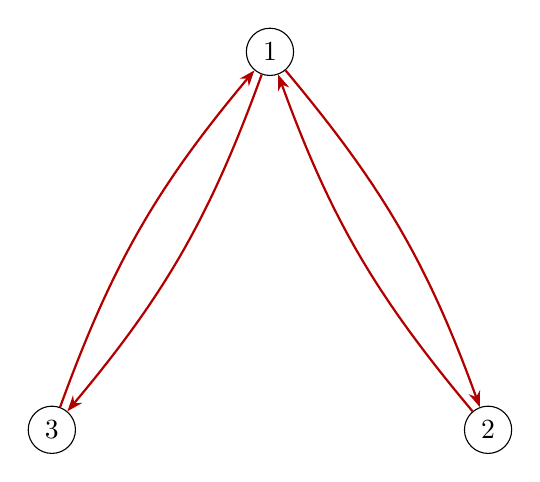
\begin{tikzpicture}[>={Stealth[length=2mm]}]
\node[draw,circle,minimum size=6mm,inner sep=0pt] (n0) at (0.00,3.20) {1};
\node[draw,circle,minimum size=6mm,inner sep=0pt] (n1) at (2.77,-1.60) {2};
\node[draw,circle,minimum size=6mm,inner sep=0pt] (n2) at (-2.77,-1.60) {3};
\draw[->,red!70!black,thick] (n0) to[bend left=10] (n1);
\draw[->,red!70!black,thick] (n0) to[bend left=10] (n2);
\draw[->,red!70!black,thick] (n1) to[bend left=10] (n0);
\draw[->,red!70!black,thick] (n2) to[bend left=10] (n0);
\end{tikzpicture}
\end{center}
\noindent Solid: defeats. Dashed: supports. Dotted: one party's case is part of another's.
\begin{enumerate}
\item Luther on ‘her seed’: the wording itself signifies no human father
\item Leupold on ‘her seed’: her posterity, named for the deception
\item Lewis on ‘her seed’: Genesis says it of Hagar and Rebekah too
\end{enumerate}
\begin{longtable}{@{}>{\raggedright\arraybackslash}p{0.3\textwidth} >{\raggedright\arraybackslash}p{0.3\textwidth} >{\raggedright\arraybackslash}p{0.3\textwidth}@{}}
\toprule
\textbf{From} & \textbf{To} & \textbf{Edge} \\
\midrule
\endhead
1 \emph{Luther on ‘her seed’: the wording itself signifies no human father} & 2 \emph{Leupold on ‘her seed’: her posterity, named for the deception} & defeats \\
1 \emph{Luther on ‘her seed’: the wording itself signifies no human father} & 3 \emph{Lewis on ‘her seed’: Genesis says it of Hagar and Rebekah too} & defeats \\
2 \emph{Leupold on ‘her seed’: her posterity, named for the deception} & 1 \emph{Luther on ‘her seed’: the wording itself signifies no human father} & defeats \\
3 \emph{Lewis on ‘her seed’: Genesis says it of Hagar and Rebekah too} & 1 \emph{Luther on ‘her seed’: the wording itself signifies no human father} & defeats \\
\bottomrule
\end{longtable}
\noindent The defeats are the cells of \texttt{genesis\allowbreak{}Dispute\_\allowbreak{}defeats}, the supports the cells of \texttt{genesis\allowbreak{}Dispute\_\allowbreak{}supports} and the parts the cells of \texttt{genesis\allowbreak{}Dispute\_\allowbreak{}part\allowbreak{}Of}, each computed from the parties' premises and checked by the kernel. The attacks derived through support and through parts are reported, not counted: every verdict is computed from the defeats alone. Every derived attack is already a defeat.
\par\medskip\noindent\textbf{\texttt{posterity\_\allowbreak{}stands\_\allowbreak{}with\_\allowbreak{}the\_\allowbreak{}idiom}}\par\nobreak\noindent
\textbf{Leupold and Lewis stand together}, on Leupold’s reading, in which Lewis’s claims hold too.

{\small\begin{verbatim}
theorem posterity_stands_with_the_idiom : genesisDispute.StandTogether
    [GenesisParty.posterity, GenesisParty.idiom]
-- axioms: propext, Classical.choice, Quot.sound
\end{verbatim}}
\par\medskip\noindent\textbf{\texttt{every\allowbreak{}Genesis\allowbreak{}Party\allowbreak{}Defeated}}\par\nobreak\noindent
Why nothing prevails: a defeater for each party.

\paragraph{Nothing prevails outright: every party is defeated by another.}
\begin{itemize}
\item \emph{Leupold on ‘her seed’: her posterity, named for the deception} defeats \emph{Luther on ‘her seed’: the wording itself signifies no human father}.
\item \emph{Luther on ‘her seed’: the wording itself signifies no human father} defeats \emph{Leupold on ‘her seed’: her posterity, named for the deception}.
\item \emph{Luther on ‘her seed’: the wording itself signifies no human father} defeats \emph{Lewis on ‘her seed’: Genesis says it of Hagar and Rebekah too}.
\end{itemize}
\par\noindent\textbf{What this rests on.} The reasons state 3 defeats and 0 absences of defeat, each a cell of the defeat table, \texttt{genesis\allowbreak{}Dispute\_\allowbreak{}defeats}, computed from the two parties' premises and checked by the kernel. Whether an attack survives turns on the attacker's weakest link and on the rating of what it attacks, so a changed rating can change the verdict. The weakest links:
\begin{itemize}
\item \emph{Leupold on ‘her seed’: her posterity, named for the deception}, weakest at \emph{disputed}:
\begin{itemize}
\item ‘Her seed’ at Genesis 3:15 is first collective: her posterity, not one person --- \cite[167--169]{leupold-exposition-genesis-1942}; \cite[170]{calvin-commentary-genesis-1847}; \cite[101]{keil-delitzsch-pentateuch-1866}; \cite[145--146]{collins-syntactical-note-1997}
\item an inference step --- \cite[169]{leupold-exposition-genesis-1942}; \cite[101--102]{keil-delitzsch-pentateuch-1866}; \cite[170]{calvin-commentary-genesis-1847}; \cite[III.23.7]{irenaeus-against-heresies-180}; \cite[V.21.1]{irenaeus-against-heresies-180}; \cite[ad loc. Gen 3:15]{henry-commentary-whole-bible}
\end{itemize}
\item \emph{Luther on ‘her seed’: the wording itself signifies no human father}, weakest at \emph{disputed}:
\begin{itemize}
\item Genesis 3:15 is the protoevangelium, the first promise of a redeemer --- \cite[167]{leupold-exposition-genesis-1942}; \cite[102]{keil-delitzsch-pentateuch-1866}; \cite{miravalle-meet-your-mother-2014}; \cite[318]{lewis-womans-seed-1991}
\item an inference step --- \cite[298--299]{luther-on-the-creation-1904}; \cite[ad loc. Gen 3:15]{henry-commentary-whole-bible}; \cite[167--169]{leupold-exposition-genesis-1942}; \cite[102]{keil-delitzsch-pentateuch-1866}; \cite[319]{lewis-womans-seed-1991}
\end{itemize}
\item \emph{Lewis on ‘her seed’: Genesis says it of Hagar and Rebekah too}, weakest at \emph{disputed}:
\begin{itemize}
\item an inference step --- \cite[299--300]{lewis-womans-seed-1991}; \cite[319]{lewis-womans-seed-1991}; \cite{akin-woman-seed-serpent-1999}
\end{itemize}
\end{itemize}
\par\medskip\noindent\textbf{\texttt{nothing\_\allowbreak{}prevails\_\allowbreak{}over\_\allowbreak{}her\_\allowbreak{}seed}}\par\nobreak\noindent
\textbf{Nothing prevails.} Every party is defeated by someone — Luther by Leupold and by Lewis, each of them by Luther — so no position is accepted however the standoffs are resolved.

{\small\begin{verbatim}
theorem nothing_prevails_over_her_seed : Framework.grounded
    genesisDispute.defeats = ∅
-- axioms: propext, Classical.choice, Quot.sound
\end{verbatim}}
\par\medskip\noindent\textbf{\texttt{wording\allowbreak{}Alone}}\par\nobreak\noindent
Why Luther alone is one resolution.

\paragraph{A maximal defensible position: \emph{Luther on ‘her seed’: the wording itself signifies no human father}.}
\begin{itemize}
\item \emph{Luther on ‘her seed’: the wording itself signifies no human father} does not defeat itself, and answers each attack on it:
\begin{itemize}
\item \emph{Leupold on ‘her seed’: her posterity, named for the deception} defeats \emph{Luther on ‘her seed’: the wording itself signifies no human father}, and \emph{Luther on ‘her seed’: the wording itself signifies no human father} defeats \emph{Leupold on ‘her seed’: her posterity, named for the deception}.
\item \emph{Lewis on ‘her seed’: Genesis says it of Hagar and Rebekah too} defeats \emph{Luther on ‘her seed’: the wording itself signifies no human father}, and \emph{Luther on ‘her seed’: the wording itself signifies no human father} defeats \emph{Lewis on ‘her seed’: Genesis says it of Hagar and Rebekah too}.
\end{itemize}
\item Nothing can be added to it:
\begin{itemize}
\item \emph{Leupold on ‘her seed’: her posterity, named for the deception} conflicts with \emph{Luther on ‘her seed’: the wording itself signifies no human father}: \emph{Leupold on ‘her seed’: her posterity, named for the deception} defeats \emph{Luther on ‘her seed’: the wording itself signifies no human father}, and \emph{Luther on ‘her seed’: the wording itself signifies no human father} defeats \emph{Leupold on ‘her seed’: her posterity, named for the deception}.
\item \emph{Lewis on ‘her seed’: Genesis says it of Hagar and Rebekah too} conflicts with \emph{Luther on ‘her seed’: the wording itself signifies no human father}: \emph{Lewis on ‘her seed’: Genesis says it of Hagar and Rebekah too} defeats \emph{Luther on ‘her seed’: the wording itself signifies no human father}, and \emph{Luther on ‘her seed’: the wording itself signifies no human father} defeats \emph{Lewis on ‘her seed’: Genesis says it of Hagar and Rebekah too}.
\end{itemize}
\end{itemize}
\par\noindent\textbf{What this rests on.} The reasons state 4 defeats and 1 absence of defeat, each a cell of the defeat table, \texttt{genesis\allowbreak{}Dispute\_\allowbreak{}defeats}, computed from the two parties' premises and checked by the kernel. Whether an attack survives turns on the attacker's weakest link and on the rating of what it attacks, so a changed rating can change the verdict. The weakest links:
\begin{itemize}
\item \emph{Luther on ‘her seed’: the wording itself signifies no human father}, weakest at \emph{disputed}:
\begin{itemize}
\item Genesis 3:15 is the protoevangelium, the first promise of a redeemer --- \cite[167]{leupold-exposition-genesis-1942}; \cite[102]{keil-delitzsch-pentateuch-1866}; \cite{miravalle-meet-your-mother-2014}; \cite[318]{lewis-womans-seed-1991}
\item an inference step --- \cite[298--299]{luther-on-the-creation-1904}; \cite[ad loc. Gen 3:15]{henry-commentary-whole-bible}; \cite[167--169]{leupold-exposition-genesis-1942}; \cite[102]{keil-delitzsch-pentateuch-1866}; \cite[319]{lewis-womans-seed-1991}
\end{itemize}
\item \emph{Leupold on ‘her seed’: her posterity, named for the deception}, weakest at \emph{disputed}:
\begin{itemize}
\item ‘Her seed’ at Genesis 3:15 is first collective: her posterity, not one person --- \cite[167--169]{leupold-exposition-genesis-1942}; \cite[170]{calvin-commentary-genesis-1847}; \cite[101]{keil-delitzsch-pentateuch-1866}; \cite[145--146]{collins-syntactical-note-1997}
\item an inference step --- \cite[169]{leupold-exposition-genesis-1942}; \cite[101--102]{keil-delitzsch-pentateuch-1866}; \cite[170]{calvin-commentary-genesis-1847}; \cite[III.23.7]{irenaeus-against-heresies-180}; \cite[V.21.1]{irenaeus-against-heresies-180}; \cite[ad loc. Gen 3:15]{henry-commentary-whole-bible}
\end{itemize}
\item \emph{Lewis on ‘her seed’: Genesis says it of Hagar and Rebekah too}, weakest at \emph{disputed}:
\begin{itemize}
\item an inference step --- \cite[299--300]{lewis-womans-seed-1991}; \cite[319]{lewis-womans-seed-1991}; \cite{akin-woman-seed-serpent-1999}
\end{itemize}
\end{itemize}
\par\medskip\noindent\textbf{\texttt{wording\_\allowbreak{}is\_\allowbreak{}one\_\allowbreak{}resolution}}\par\nobreak\noindent
\textbf{One resolution: Luther.} His case can be defended on its own, because it defeats both parties that defeat it; and it is in conflict with both, so no larger set can be defended.

{\small\begin{verbatim}
theorem wording_is_one_resolution : Framework.Preferred genesisDispute.defeats
    {GenesisParty.wording}
-- axioms: propext, Classical.choice, Quot.sound
\end{verbatim}}
\par\medskip\noindent\textbf{\texttt{posterity\allowbreak{}With\allowbreak{}The\allowbreak{}Idiom}}\par\nobreak\noindent
Why Leupold with Lewis is the other resolution.

\paragraph{A maximal defensible position: \emph{Leupold on ‘her seed’: her posterity, named for the deception}, \emph{Lewis on ‘her seed’: Genesis says it of Hagar and Rebekah too}.}
\begin{itemize}
\item None of \emph{Leupold on ‘her seed’: her posterity, named for the deception}, \emph{Lewis on ‘her seed’: Genesis says it of Hagar and Rebekah too} defeats another, and each attack on them is answered from among them:
\begin{itemize}
\item \emph{Luther on ‘her seed’: the wording itself signifies no human father} defeats \emph{Leupold on ‘her seed’: her posterity, named for the deception}, and \emph{Leupold on ‘her seed’: her posterity, named for the deception} defeats \emph{Luther on ‘her seed’: the wording itself signifies no human father}.
\item \emph{Luther on ‘her seed’: the wording itself signifies no human father} defeats \emph{Lewis on ‘her seed’: Genesis says it of Hagar and Rebekah too}, and \emph{Leupold on ‘her seed’: her posterity, named for the deception} defeats \emph{Luther on ‘her seed’: the wording itself signifies no human father}.
\end{itemize}
\item Nothing can be added to it:
\begin{itemize}
\item \emph{Luther on ‘her seed’: the wording itself signifies no human father} conflicts with \emph{Leupold on ‘her seed’: her posterity, named for the deception}: \emph{Luther on ‘her seed’: the wording itself signifies no human father} defeats \emph{Leupold on ‘her seed’: her posterity, named for the deception}, and \emph{Leupold on ‘her seed’: her posterity, named for the deception} defeats \emph{Luther on ‘her seed’: the wording itself signifies no human father}.
\end{itemize}
\end{itemize}
\par\noindent\textbf{What this rests on.} The reasons state 3 defeats and 4 absences of defeat, each a cell of the defeat table, \texttt{genesis\allowbreak{}Dispute\_\allowbreak{}defeats}, computed from the two parties' premises and checked by the kernel. Whether an attack survives turns on the attacker's weakest link and on the rating of what it attacks, so a changed rating can change the verdict. The weakest links:
\begin{itemize}
\item \emph{Leupold on ‘her seed’: her posterity, named for the deception}, weakest at \emph{disputed}:
\begin{itemize}
\item ‘Her seed’ at Genesis 3:15 is first collective: her posterity, not one person --- \cite[167--169]{leupold-exposition-genesis-1942}; \cite[170]{calvin-commentary-genesis-1847}; \cite[101]{keil-delitzsch-pentateuch-1866}; \cite[145--146]{collins-syntactical-note-1997}
\item an inference step --- \cite[169]{leupold-exposition-genesis-1942}; \cite[101--102]{keil-delitzsch-pentateuch-1866}; \cite[170]{calvin-commentary-genesis-1847}; \cite[III.23.7]{irenaeus-against-heresies-180}; \cite[V.21.1]{irenaeus-against-heresies-180}; \cite[ad loc. Gen 3:15]{henry-commentary-whole-bible}
\end{itemize}
\item \emph{Lewis on ‘her seed’: Genesis says it of Hagar and Rebekah too}, weakest at \emph{disputed}:
\begin{itemize}
\item an inference step --- \cite[299--300]{lewis-womans-seed-1991}; \cite[319]{lewis-womans-seed-1991}; \cite{akin-woman-seed-serpent-1999}
\end{itemize}
\item \emph{Luther on ‘her seed’: the wording itself signifies no human father}, weakest at \emph{disputed}:
\begin{itemize}
\item Genesis 3:15 is the protoevangelium, the first promise of a redeemer --- \cite[167]{leupold-exposition-genesis-1942}; \cite[102]{keil-delitzsch-pentateuch-1866}; \cite{miravalle-meet-your-mother-2014}; \cite[318]{lewis-womans-seed-1991}
\item an inference step --- \cite[298--299]{luther-on-the-creation-1904}; \cite[ad loc. Gen 3:15]{henry-commentary-whole-bible}; \cite[167--169]{leupold-exposition-genesis-1942}; \cite[102]{keil-delitzsch-pentateuch-1866}; \cite[319]{lewis-womans-seed-1991}
\end{itemize}
\end{itemize}
\par\medskip\noindent\textbf{\texttt{posterity\_\allowbreak{}and\_\allowbreak{}idiom\_\allowbreak{}are\_\allowbreak{}the\_\allowbreak{}other\_\allowbreak{}resolution}}\par\nobreak\noindent
\textbf{The other resolution: Leupold, with Lewis.} Neither defeats the other, and each answers Luther, the only party to defeat either. Luther is in conflict with both, so no larger set can be defended.

{\small\begin{verbatim}
theorem posterity_and_idiom_are_the_other_resolution : Framework.Preferred
    genesisDispute.defeats {GenesisParty.posterity, GenesisParty.idiom}
-- axioms: propext, Classical.choice, Quot.sound
\end{verbatim}}
\par\medskip\noindent\textbf{\texttt{wording\_\allowbreak{}not\_\allowbreak{}skeptically\_\allowbreak{}accepted}}\par\nobreak\noindent
So the dispute does not force Luther’s reading.

{\small\begin{verbatim}
theorem wording_not_skeptically_accepted : ¬Framework.SkepticallyAccepted
    genesisDispute.defeats GenesisParty.wording
-- axioms: propext, Classical.choice, Quot.sound
\end{verbatim}}
\par\medskip\noindent\textbf{\texttt{posterity\_\allowbreak{}not\_\allowbreak{}skeptically\_\allowbreak{}accepted}}\par\nobreak\noindent
Nor does it force Leupold’s.

{\small\begin{verbatim}
theorem posterity_not_skeptically_accepted : ¬Framework.SkepticallyAccepted
    genesisDispute.defeats GenesisParty.posterity
-- axioms: propext, Classical.choice, Quot.sound
\end{verbatim}}
\subsection*{Is Genesis 3:15 a promise, fulfilled in Jesus?}
\addcontentsline{toc}{subsection}{Is Genesis 3:15 a promise, fulfilled in Jesus?}
The chapter “Does Genesis 3:15 rule out a human father?” asks what the wording of Genesis 3:15 says of a father. A reader of the whole Bible asks the next question. In the garden God tells the serpent that the woman’s seed will crush its head, and that it will strike his heel. The Gospel tells of one born of a woman, struck in his death, who destroyed the devil through it. \textbf{Is the promise fulfilled in him, and does the fulfilment confirm that it was a promise?}

\subsubsection*{The terms of the promise, and where Scripture says they are met}
\begin{longtable}{@{}>{\raggedright\arraybackslash}p{0.45\textwidth} >{\raggedright\arraybackslash}p{0.45\textwidth}@{}}
\toprule
\textbf{Genesis 3:15} & \textbf{Where the New Testament names it} \\
\midrule
\endhead
The woman’s seed & The Son “made of a woman” (Galatians 4:4) \\
The serpent & “that old serpent, called the Devil, and Satan” (Revelation 12:9; 20:2) \\
His head crushed & “that through death he might destroy … the devil” (Hebrews 2:14; 1 John 3:8) \\
His heel struck & He died, and rose the third day (1 Corinthians 15:3–4) \\
\bottomrule
\end{longtable}
Romans 16:20, “the God of peace shall bruise Satan under your feet shortly”, is left out: it is an allusion, and a disputed one (\texttt{fulfilment\allowbreak{}Line} gives both sides).

\subsubsection*{Four positions}
\begin{itemize}
  \item \textbf{The fulfilment, confirming the promise} (\texttt{fulfilment\allowbreak{}Case}). From the terms met (\texttt{fulfilment\allowbreak{}Line}): in Jesus the promise is fulfilled. From the fulfilment (\texttt{confirmation\allowbreak{}Line}): the verse was a promise of him, the protoevangelium. Its grounds are Scripture alone.
  \item \textbf{Westermann’s denial} (\texttt{westermann\allowbreak{}Case}), encoded first: “her seed” is a line of descendants, and the verse is a punishment oracle on the serpent, a form that cannot carry “promise or prophecy as its primary or even as its secondary meaning” (\emph{Genesis 1–11}, 259–60).
  \item \textbf{The syntax of the striker} (\texttt{syntax\allowbreak{}Case}), against Westermann’s first ground: elsewhere זֶרַע with singular verbs and pronouns names one descendant, at 3:15b it is “he” who strikes the serpent’s own head, and the Greek translator read one person; so “her seed” is not only a line of descendants (Collins, Alexander, Leupold, Hamilton).
  \item \textbf{The scene read whole} (\texttt{scene\allowbreak{}Case}): the serpent speaks and twists God’s command, as no animal does of itself; it is the instrument of an evil power; the blow falls on the serpent itself; and God sets the enmity. So the sentence on the serpent is a promise of victory over that power (Collins, Woudstra, Keil).
\end{itemize}
The readers before Christ do not read the verse so. Jubilees, Philo and Josephus read the serpent as an animal or an emblem, and none of them reads the verse as a promise. The scene’s reading is an exegesis of the section, from its own words.

\subsubsection*{What the confirmation shows, and what it does not}
The fulfilment confirms the promise; it does not prove it from Genesis alone. “If the verse promised the Messiah, he would crush the serpent and be struck; Jesus did; so it promised him” would affirm the consequent. What the library encodes is a step of its own, rated: a promise whose every term is met in one person, as Scripture names them, is a promise of that person. It holds for a reader who denies the virginal conception (\texttt{the\_\allowbreak{}confirmation\_\allowbreak{}does\_\allowbreak{}not\_\allowbreak{}need\_\allowbreak{}the\_\allowbreak{}virgin\_\allowbreak{}birth}).

Joined with the virginal conception, the fulfilment says one thing more: the seed in whom the promise is fulfilled was of the woman alone (\texttt{seed\_\allowbreak{}of\_\allowbreak{}the\_\allowbreak{}woman\_\allowbreak{}alone}). That reads the birth back into the promise. It does not show that the wording foretold it, which is Luther’s claim and is weighed in the chapter “Does Genesis 3:15 rule out a human father?” (\texttt{the\_\allowbreak{}fulfilment\_\allowbreak{}does\_\allowbreak{}not\_\allowbreak{}reach\_\allowbreak{}the\_\allowbreak{}wording}).

\subsubsection*{How the ratings stand, and what the solver computes}
\begin{itemize}
  \item \textbf{The fulfilment’s step} is \texttt{disputed}, on Westermann. He grants what every ground reads and denies the conclusion, “even as its secondary meaning”, from philology and form criticism, not from a reading of the New Testament texts.
  \item \textbf{The confirmation’s step} is \texttt{plausible}: no reader found grants the fulfilment and denies the promise.
  \item \textbf{Westermann’s step} is \texttt{disputed}, on Calvin, who grants that the seed is the woman’s posterity and the verse a curse on the serpent, and finds the promise in the curse; and Keil with him.
  \item \textbf{Westermann’s first ground}, “a line of descendants and not an individual”, is \texttt{disputed} too, on Collins, Leupold, Alexander and Hamilton.
  \item \textbf{The scene’s step} is \texttt{plausible}: Woudstra grants every ground and holds that “the term ‘protevangelium’ may be rightly used”. Its ground that the serpent is the instrument of an evil power is \texttt{disputed}, on Westermann.
  \item \textbf{The syntax’s step} is \texttt{disputed}, on Keil, who grants that the word can name one son and that the victory is over the serpent itself, and denies “one individual only”. Collins himself claims no more than that the syntax is “quite consistent with” one person.
\end{itemize}
Each position is only as strong as its weakest link, and each rests on a step rated \texttt{disputed}. Westermann and the fulfilment defeat each other, and so do Westermann and the scene; Westermann and the syntax defeat each other, the syntax by denying his ground; the fulfilment, the syntax and the scene stand together. So \textbf{nothing prevails} (\texttt{nothing\_\allowbreak{}prevails\_\allowbreak{}over\_\allowbreak{}the\_\allowbreak{}promise}). The fulfilment with the syntax and the scene can be defended (\texttt{fulfilment\_\allowbreak{}is\_\allowbreak{}one\_\allowbreak{}resolution}), and so can Westermann (\texttt{westermann\_\allowbreak{}is\_\allowbreak{}the\_\allowbreak{}other\_\allowbreak{}resolution}); neither is forced.

That is the verdict as the evidence weighs it. Whether Westermann’s dissent should be heard against a step whose grounds are all Scripture is a question of standard, not of evidence, and the dispute is heard under each standard below.

\subsubsection*{The promise, heard under each standard}
The dispute above weighs the fulfilment of Genesis 3:15 against Westermann’s denial that the verse is any promise, and as the evidence weighs it nothing prevails. That verdict leaves a question open: \textbf{should Westermann’s dissent be heard against a step whose grounds are all Scripture?}

The fulfilment’s step rests on five texts, each a claim about what Scripture says: Genesis 3:15 itself, Galatians 4:4, Revelation 12:9, Hebrews 2:14 with 1 John 3:8, and 1 Corinthians 15:3–4. Westermann grants every one of them, and denies the step from an argument of his own: “her seed” is “a line of descendants and not an individual” (259), and the verse is a punishment oracle, a form that cannot carry promise “even as its secondary meaning” (260). His first ground is philology; it is not a reading of another text of Scripture.

\subsubsection*{Under each standard}
The library computes the answer under every standard it knows (\texttt{Testimony.Logic.Credibility}), and reports each.

\begin{itemize}
  \item \textbf{Under the evidence standard} Westermann’s dissent is a credible critique: consistent, granting the fulfilment’s grounds, argued by a step of his own, and resting on what anyone can check. The fulfilment’s step is \texttt{disputed}, and the hearing is the dispute as it stands: \textbf{nothing prevails}.
  \item \textbf{Under the tradition standard}, the same.
  \item \textbf{Under the Scripture standard} a dissent from a step whose grounds are all Scripture must itself rest on Scripture alone, and Westermann’s rests on his reading of the Hebrew word. So he is not heard; the fulfilment’s step stands at the confidence its support is cited at, \texttt{plausible}; and \textbf{the fulfilment prevails, with the syntax of the striker and the scene read whole} (\texttt{promise\_\allowbreak{}turns\_\allowbreak{}on\_\allowbreak{}the\_\allowbreak{}standard}).
\end{itemize}
\subsubsection*{What the hearing does not do}
A dissent not heard under a standard is not heard at all: the hearing sets the party aside, not one attack of his. So under the Scripture standard Westermann’s denial that an evil power stands behind the serpent, a ground of the scene’s, is not weighed either, and that ground stays rated \texttt{disputed} in its citation. And the Scripture standard silences no dissent that argues from Scripture: another text, read the other way, would be heard.

Nor does the verdict say what Genesis 3:15 meant to its first readers. The readers before Christ do not read it as a promise of one victor (see the dispute above). It says what the verse is, read with the rest of Scripture, for a reader who holds that Scripture interprets Scripture.

\subsubsection*{How this is checked}
\paragraph*{Readings}
\leavevmode\par\nobreak
\par\medskip\noindent\textbf{\texttt{westermann\allowbreak{}Reading}}\par\nobreak\noindent
Westermann’s reading: “her seed” is the woman’s posterity, the verse is the serpent’s sentence and no promise, and so no one fulfils it. On the joined pairs elsewhere in the argument it takes the scriptural reading’s side, as the readings of \texttt{Results.Genesis} do; none bears on what it is used for.

{\small\begin{verbatim}
def westermannReading : Valuation Claim :=
  fun a =>
    match a with
    | Claim.genesis3_15IsProtoevangelium => False
    | Claim.jesusFulfilsThePromise => False
    | Claim.seedWasOfTheWomanAlone => False
    | Claim.wordingSignifiesAFatherlessBirth => False
    | Claim.serpentIsTheInstrumentOfAPower => False
    | Claim.parthenosMeantYoungWoman => False
    | Claim.parthenosDoesNotItselfConnoteVirginity => False
    | Claim.parthenosDescribesDinahAsSheThenWas => False
    | Claim.maternalSilenceProvesNothing => False
    | Claim.magisteriumIsDoctrinallyAuthoritative => False
    | x => True
\end{verbatim}}
\par\medskip\noindent\textbf{\texttt{curse\allowbreak{}Without\allowbreak{}Promise\allowbreak{}Reading}}\par\nobreak\noindent
A reading no cited reader holds, written down to show what the scene’s step adds: the serpent twists the command, an evil power stands behind it, the blow falls on the serpent itself and God sets the enmity — and still the verse is no promise, and no one fulfils it. It is a model of the scene’s grounds without its step.

{\small\begin{verbatim}
def curseWithoutPromiseReading : Valuation Claim :=
  fun a =>
    match a with
    | Claim.genesis3_15IsProtoevangelium => False
    | Claim.jesusFulfilsThePromise => False
    | Claim.seedWasOfTheWomanAlone => False
    | Claim.wordingSignifiesAFatherlessBirth => False
    | Claim.parthenosMeantYoungWoman => False
    | Claim.parthenosDoesNotItselfConnoteVirginity => False
    | Claim.parthenosDescribesDinahAsSheThenWas => False
    | Claim.maternalSilenceProvesNothing => False
    | Claim.magisteriumIsDoctrinallyAuthoritative => False
    | x => True
\end{verbatim}}
\par\medskip\noindent\textbf{\texttt{calvin\allowbreak{}Reading}}\par\nobreak\noindent
Calvin’s reading: “her seed” is “the posterity of the woman generally”, and not one man; the verse is the serpent’s sentence; and the promise is in it all the same, for “we must necessarily come to one head” (170–71). On the other joined pairs it takes the scriptural reading’s side.

{\small\begin{verbatim}
def calvinReading : Valuation Claim :=
  fun a =>
    match a with
    | Claim.wordingSignifiesAFatherlessBirth => False
    | Claim.parthenosMeantYoungWoman => False
    | Claim.parthenosDoesNotItselfConnoteVirginity => False
    | Claim.parthenosDescribesDinahAsSheThenWas => False
    | Claim.maternalSilenceProvesNothing => False
    | Claim.magisteriumIsDoctrinallyAuthoritative => False
    | x => True
\end{verbatim}}
\paragraph*{The fulfilment, the confirmation, and the seed of the woman alone}
\leavevmode\par\nobreak
\par\medskip\noindent\textbf{\texttt{fulfilment\allowbreak{}Case\_\allowbreak{}establishes}}\par\nobreak\noindent
\textbf{The fulfilment confirms the promise.} Grant what the five texts read, the fulfilment’s step and the confirmation’s: Genesis 3:15 is the protoevangelium.

{\small\begin{verbatim}
theorem fulfilmentCase_establishes : Establishes fulfilmentCase
-- axioms: propext, Quot.sound
\end{verbatim}}
\par\medskip\noindent\textbf{\texttt{fulfilment\allowbreak{}Case\_\allowbreak{}is\_\allowbreak{}satisfiable}}\par\nobreak\noindent
The fulfilment’s premises can all be true together, on Luther’s reading, which grants every term met, the promise fulfilled and confirmed.

{\small\begin{verbatim}
theorem fulfilmentCase_is_satisfiable : Satisfiable fulfilmentCase.premises
-- axioms: propext, Quot.sound
\end{verbatim}}
\par\medskip\noindent\textbf{\texttt{the\_\allowbreak{}fulfilment\_\allowbreak{}rests\_\allowbreak{}on\_\allowbreak{}its\_\allowbreak{}step}}\par\nobreak\noindent
\textbf{The fulfilment rests on its step.} Grant everything the five texts say: on Westermann’s reading the verse still promises no one, and so no one fulfils it. The texts do not settle it; the step does, and that is why it is rated \texttt{disputed}.

{\small\begin{verbatim}
theorem the_fulfilment_rests_on_its_step : ¬Entails fulfilmentLine.grounds (p
    Claim.jesusFulfilsThePromise)
-- axioms: propext, Quot.sound
\end{verbatim}}
\par\medskip\noindent\textbf{\texttt{the\_\allowbreak{}confirmation\_\allowbreak{}does\_\allowbreak{}not\_\allowbreak{}need\_\allowbreak{}the\_\allowbreak{}virgin\_\allowbreak{}birth}}\par\nobreak\noindent
\textbf{The confirmation does not need the virgin birth.} The promise follows from the fulfilment even for a reader who denies the virginal conception: none of the fulfilment’s grounds is the birth, and none of its steps uses it.

{\small\begin{verbatim}
theorem the_confirmation_does_not_need_the_virgin_birth : Entails
    (fulfilmentCase.premises ++ [notP Claim.maryConceivedAsVirgin]) (p
    Claim.genesis3_15IsProtoevangelium)
-- axioms: propext, Quot.sound
\end{verbatim}}
\par\medskip\noindent\textbf{\texttt{seed\_\allowbreak{}of\_\allowbreak{}the\_\allowbreak{}woman\_\allowbreak{}alone}}\par\nobreak\noindent
\textbf{The seed of the woman alone.} Grant the fulfilment and the virginal conception: the seed in whom Genesis 3:15 is fulfilled had no human father.

{\small\begin{verbatim}
theorem seed_of_the_woman_alone : Establishes aloneCase
-- axioms: propext, Quot.sound
\end{verbatim}}
\par\medskip\noindent\textbf{\texttt{alone\allowbreak{}Case\_\allowbreak{}is\_\allowbreak{}satisfiable}}\par\nobreak\noindent
The premises of the seed of the woman alone can all be true together, on Luther’s reading.

{\small\begin{verbatim}
theorem aloneCase_is_satisfiable : Satisfiable aloneCase.premises
-- axioms: propext, Quot.sound
\end{verbatim}}
\par\medskip\noindent\textbf{\texttt{the\_\allowbreak{}fulfilment\_\allowbreak{}does\_\allowbreak{}not\_\allowbreak{}reach\_\allowbreak{}the\_\allowbreak{}wording}}\par\nobreak\noindent
\textbf{The fulfilment does not reach the wording.} Grant the fulfilment, the confirmation, the virginal conception and the seed of the woman alone: the wording of Genesis 3:15 may still not itself signify a birth with no human father, as Leupold reads it. Reading the birth back into the promise is not finding it in the words; Luther’s claim stands or falls in \texttt{Dispute.Genesis}.

{\small\begin{verbatim}
theorem the_fulfilment_does_not_reach_the_wording : ¬Entails
    (fulfilmentCase.premises ++ aloneCase.premises) (p
    Claim.wordingSignifiesAFatherlessBirth)
-- axioms: propext, Quot.sound
\end{verbatim}}
\paragraph*{Westermann’s denial}
\leavevmode\par\nobreak
\par\medskip\noindent\textbf{\texttt{westermann\allowbreak{}Case\_\allowbreak{}establishes}}\par\nobreak\noindent
Westermann’s denial delivers its conclusion.

{\small\begin{verbatim}
theorem westermannCase_establishes : Establishes westermannCase
-- axioms: propext, Quot.sound
\end{verbatim}}
\par\medskip\noindent\textbf{\texttt{westermann\allowbreak{}Case\_\allowbreak{}is\_\allowbreak{}satisfiable}}\par\nobreak\noindent
Westermann’s premises can all be true together: his own reading.

{\small\begin{verbatim}
theorem westermannCase_is_satisfiable : Satisfiable westermannCase.premises
-- axioms: propext, Quot.sound
\end{verbatim}}
\par\medskip\noindent\textbf{\texttt{westermann\_\allowbreak{}rests\_\allowbreak{}on\_\allowbreak{}his\_\allowbreak{}step}}\par\nobreak\noindent
\textbf{Westermann’s denial rests on its step.} Grant that “her seed” is a line of descendants and not one man, and that the verse is a curse on the serpent: on Calvin’s reading the verse is a promise all the same.

{\small\begin{verbatim}
theorem westermann_rests_on_his_step : ¬Entails westermannLine.grounds (notP
    Claim.genesis3_15IsProtoevangelium)
-- axioms: propext, Quot.sound
\end{verbatim}}
\paragraph*{The syntax of the striker}
\leavevmode\par\nobreak
\par\medskip\noindent\textbf{\texttt{syntax\allowbreak{}Case\_\allowbreak{}establishes}}\par\nobreak\noindent
The syntax’s case delivers its conclusion.

{\small\begin{verbatim}
theorem syntaxCase_establishes : Establishes syntaxCase
-- axioms: propext, Quot.sound
\end{verbatim}}
\par\medskip\noindent\textbf{\texttt{syntax\allowbreak{}Case\_\allowbreak{}is\_\allowbreak{}satisfiable}}\par\nobreak\noindent
The syntax’s premises can all be true together, on Leupold’s reading.

{\small\begin{verbatim}
theorem syntaxCase_is_satisfiable : Satisfiable syntaxCase.premises
-- axioms: propext, Quot.sound
\end{verbatim}}
\par\medskip\noindent\textbf{\texttt{syntax\_\allowbreak{}rests\_\allowbreak{}on\_\allowbreak{}its\_\allowbreak{}step}}\par\nobreak\noindent
\textbf{The syntax rests on its step.} Grant that זֶרַע names one descendant elsewhere with singular forms, that the striker at 3:15b is singular “he”, and that the Greek translator read one person: on Calvin’s reading “her seed” is still the woman’s posterity, and not one man.

{\small\begin{verbatim}
theorem syntax_rests_on_its_step : ¬Entails syntaxLine.grounds (notP
    Claim.seedIsLineNotIndividual)
-- axioms: propext, Quot.sound
\end{verbatim}}
\paragraph*{The scene read whole}
\leavevmode\par\nobreak
\par\medskip\noindent\textbf{\texttt{scene\allowbreak{}Case\_\allowbreak{}establishes}}\par\nobreak\noindent
The scene’s case delivers its conclusion.

{\small\begin{verbatim}
theorem sceneCase_establishes : Establishes sceneCase
-- axioms: propext, Quot.sound
\end{verbatim}}
\par\medskip\noindent\textbf{\texttt{scene\allowbreak{}Case\_\allowbreak{}is\_\allowbreak{}satisfiable}}\par\nobreak\noindent
The scene’s premises can all be true together, on Luther’s reading.

{\small\begin{verbatim}
theorem sceneCase_is_satisfiable : Satisfiable sceneCase.premises
-- axioms: propext, Quot.sound
\end{verbatim}}
\par\medskip\noindent\textbf{\texttt{scene\_\allowbreak{}rests\_\allowbreak{}on\_\allowbreak{}its\_\allowbreak{}step}}\par\nobreak\noindent
\textbf{The scene rests on its step.} Grant that the serpent twists the command, that an evil power stands behind it, that the blow falls on the serpent itself, and that God sets the enmity: the verse may still be a sentence and no promise. The section’s words do not force it; reading a promise out of the curse does, and that is the step rated \texttt{plausible}.

{\small\begin{verbatim}
theorem scene_rests_on_its_step : ¬Entails sceneLine.grounds (p
    Claim.genesis3_15IsProtoevangelium)
-- axioms: propext, Quot.sound
\end{verbatim}}
\paragraph*{Strength}
\leavevmode\par\nobreak
\par\medskip\noindent\textbf{\texttt{fulfilment\allowbreak{}Case\_\allowbreak{}strength}}\par\nobreak\noindent
The fulfilment’s grounds are \texttt{consensus}, what the texts read; its confirmation is \texttt{plausible}; its fulfilment step is \texttt{disputed}, on Westermann.

{\small\begin{verbatim}
theorem fulfilmentCase_strength : fulfilmentCase.strength = 0
-- axioms: propext
\end{verbatim}}
\par\medskip\noindent\textbf{\texttt{westermann\allowbreak{}Case\_\allowbreak{}strength}}\par\nobreak\noindent
Westermann’s ground that “her seed” is a line of descendants and not an individual is \texttt{disputed}, and so is his step, on Calvin.

{\small\begin{verbatim}
theorem westermannCase_strength : westermannCase.strength = 0
-- axioms: propext
\end{verbatim}}
\par\medskip\noindent\textbf{\texttt{syntax\allowbreak{}Case\_\allowbreak{}strength}}\par\nobreak\noindent
The syntax’s grounds are \texttt{consensus} and \texttt{well\allowbreak{}Supported}, but its step is \texttt{disputed}, on Keil.

{\small\begin{verbatim}
theorem syntaxCase_strength : syntaxCase.strength = 0
-- axioms: propext
\end{verbatim}}
\par\medskip\noindent\textbf{\texttt{scene\allowbreak{}Case\_\allowbreak{}strength}}\par\nobreak\noindent
The scene’s step is \texttt{plausible}, but its ground that the serpent is the instrument of an evil power is \texttt{disputed}, on Westermann.

{\small\begin{verbatim}
theorem sceneCase_strength : sceneCase.strength = 0
-- axioms: propext
\end{verbatim}}
\paragraph*{The defeats}
\leavevmode\par\nobreak
\par\medskip\noindent\textbf{\texttt{westermann\_\allowbreak{}defeats\_\allowbreak{}fulfilment}}\par\nobreak\noindent
\textbf{Westermann defeats the fulfilment.} His conclusion denies the fulfilment’s, and the fulfilment is no stronger than he.

{\small\begin{verbatim}
theorem westermann_defeats_fulfilment : Defeats westermannCase fulfilmentCase
-- axioms: propext, Classical.choice, Quot.sound
\end{verbatim}}
\par\medskip\noindent\textbf{\texttt{fulfilment\_\allowbreak{}defeats\_\allowbreak{}westermann}}\par\nobreak\noindent
\textbf{The fulfilment defeats Westermann.} Its conclusion denies his, and he is no stronger than it.

{\small\begin{verbatim}
theorem fulfilment_defeats_westermann : Defeats fulfilmentCase westermannCase
-- axioms: propext, Classical.choice, Quot.sound
\end{verbatim}}
\paragraph*{The dispute}
\leavevmode\par\nobreak
\par\medskip\noindent\textbf{\texttt{promise\allowbreak{}Party\allowbreak{}Node}}\par\nobreak\noindent
The package each party argues from.

{\small\begin{verbatim}
def promisePartyNode : PromiseParty → ArgumentPackage Claim :=
  fun x =>
    match x with
    | PromiseParty.fulfilment => fulfilmentCase
    | PromiseParty.westermann => westermannCase
    | PromiseParty.syntax => syntaxCase
    | PromiseParty.scene => sceneCase
\end{verbatim}}
\par\medskip\noindent\textbf{\texttt{promise\allowbreak{}Dispute}}\par\nobreak\noindent
The dispute over whether Genesis 3:15 is a promise: every party’s premises have a model, every party establishes its conclusion, and every party’s inferences are rated. Every party’s weakest link ranks at the bottom.

{\small\begin{verbatim}
def promiseDispute : Dispute Claim PromiseParty :=
  { node := promisePartyNode,
    consistent := promiseDispute._proof_1,
    sound := promiseDispute._proof_2,
    rated := promiseDispute._proof_7 }
\end{verbatim}}
\par\medskip\noindent\textbf{\texttt{promise\allowbreak{}Dispute\_\allowbreak{}defeats}}\par\nobreak\noindent
\textbf{Who defeats whom}, all sixteen pairs: Westermann defeats the fulfilment, the syntax and the scene, and each defeats him back; and nothing else. Every cell is computed from what the parties hold by \texttt{Horn.defeats?} and checked by the kernel.

{\small\begin{verbatim}
theorem promiseDispute_defeats : ∀ (i j : PromiseParty),
    promiseDispute.defeats i j ↔ (i, j) ∈ [(PromiseParty.fulfilment,
    PromiseParty.westermann), (PromiseParty.westermann,
    PromiseParty.fulfilment), (PromiseParty.syntax, PromiseParty.westermann),
    (PromiseParty.westermann, PromiseParty.syntax), (PromiseParty.scene,
    PromiseParty.westermann), (PromiseParty.westermann, PromiseParty.scene)]
-- axioms: propext, Classical.choice, Quot.sound
\end{verbatim}}
\par\medskip\noindent\textbf{\texttt{promise\allowbreak{}Standoff}}\par\nobreak\noindent
Why nothing prevails: every party has a defeater.

\paragraph{Nothing prevails outright: every party is defeated by another.}
\begin{itemize}
\item \emph{Westermann: a punishment oracle on a line of descendants, and no promise} defeats \emph{The fulfilment of Genesis 3:15 confirms the promise}.
\item \emph{The fulfilment of Genesis 3:15 confirms the promise} defeats \emph{Westermann: a punishment oracle on a line of descendants, and no promise}.
\item \emph{Westermann: a punishment oracle on a line of descendants, and no promise} defeats \emph{The syntax of the striker: ‘he’ who strikes is one descendant}.
\item \emph{Westermann: a punishment oracle on a line of descendants, and no promise} defeats \emph{The scene read whole: God’s sentence on the serpent’s power}.
\end{itemize}
\par\noindent\textbf{What this rests on.} The reasons state 4 defeats and 0 absences of defeat, each a cell of the defeat table, \texttt{promise\allowbreak{}Dispute\_\allowbreak{}defeats}, computed from the two parties' premises and checked by the kernel. Whether an attack survives turns on the attacker's weakest link and on the rating of what it attacks, so a changed rating can change the verdict. The weakest links:
\begin{itemize}
\item \emph{Westermann: a punishment oracle on a line of descendants, and no promise}, weakest at \emph{disputed}:
\begin{itemize}
\item At Genesis 3:15 ‘her seed’ is a line of descendants, and not an individual --- \cite[259--260]{westermann-genesis-1-11-1984}; \cite[140, 147]{collins-syntactical-note-1997}; \cite[168]{leupold-exposition-genesis-1942}; \cite[363]{alexander-further-observations-1997}; \cite[32]{hamilton-skull-crushing-seed-2006}
\item an inference step --- \cite[259--261]{westermann-genesis-1-11-1984}; \cite[170--171]{calvin-commentary-genesis-1847}; \cite[102]{keil-delitzsch-pentateuch-1866}
\end{itemize}
\item \emph{The fulfilment of Genesis 3:15 confirms the promise}, weakest at \emph{disputed}:
\begin{itemize}
\item an inference step --- \cite[III.23.7]{irenaeus-against-heresies-180}; \cite[IV.40.3]{irenaeus-against-heresies-180}; \cite[42, 53]{hamilton-skull-crushing-seed-2006}; \cite[102]{keil-delitzsch-pentateuch-1866}; \cite[170]{leupold-exposition-genesis-1942}; \cite[170--171]{calvin-commentary-genesis-1847}; \cite[259--261]{westermann-genesis-1-11-1984}
\end{itemize}
\item \emph{The syntax of the striker: ‘he’ who strikes is one descendant}, weakest at \emph{disputed}:
\begin{itemize}
\item The Greek translator of Genesis read the woman’s seed at 3:15 as one person --- \cite[145]{collins-syntactical-note-1997}; \cite[144]{collins-syntactical-note-1997}; \cite{martin-earliest-messianic-1965}; \cite[300]{lewis-womans-seed-1991}; \cite[III.188]{philo-allegorical-interpretation-40}
\item an inference step --- \cite[144--146]{collins-syntactical-note-1997}; \cite[363, 364]{alexander-further-observations-1997}; \cite[166--168]{leupold-exposition-genesis-1942}; \cite[32]{hamilton-skull-crushing-seed-2006}; \cite[101]{keil-delitzsch-pentateuch-1866}; \cite[171]{calvin-commentary-genesis-1847}
\end{itemize}
\item \emph{The scene read whole: God’s sentence on the serpent’s power}, weakest at \emph{disputed}:
\begin{itemize}
\item The serpent of Genesis 3 is the instrument of an evil power --- \cite[146--147]{collins-syntactical-note-1997}; \cite[197]{woudstra-recent-translations-1971}; \cite[101--102]{keil-delitzsch-pentateuch-1866}; \cite[261]{westermann-genesis-1-11-1984}
\end{itemize}
\end{itemize}
\par\medskip\noindent\textbf{\texttt{nothing\_\allowbreak{}prevails\_\allowbreak{}over\_\allowbreak{}the\_\allowbreak{}promise}}\par\nobreak\noindent
\textbf{As the evidence weighs it, nothing prevails}: Westermann defeats the fulfilment, the syntax and the scene, each defeats him back, and none outranks another.

{\small\begin{verbatim}
theorem nothing_prevails_over_the_promise : Framework.grounded
    promiseDispute.defeats = ∅
-- axioms: propext, Classical.choice, Quot.sound
\end{verbatim}}
\par\medskip\noindent\textbf{\texttt{fulfilment\allowbreak{}Alone}}\par\nobreak\noindent
Why the fulfilment with the syntax and the scene is one resolution.

\paragraph{A maximal defensible position: \emph{The fulfilment of Genesis 3:15 confirms the promise}, \emph{The syntax of the striker: ‘he’ who strikes is one descendant}, \emph{The scene read whole: God’s sentence on the serpent’s power}.}
\begin{itemize}
\item None of \emph{The fulfilment of Genesis 3:15 confirms the promise}, \emph{The syntax of the striker: ‘he’ who strikes is one descendant}, \emph{The scene read whole: God’s sentence on the serpent’s power} defeats another, and each attack on them is answered from among them:
\begin{itemize}
\item \emph{Westermann: a punishment oracle on a line of descendants, and no promise} defeats \emph{The fulfilment of Genesis 3:15 confirms the promise}, and \emph{The fulfilment of Genesis 3:15 confirms the promise} defeats \emph{Westermann: a punishment oracle on a line of descendants, and no promise}.
\item \emph{Westermann: a punishment oracle on a line of descendants, and no promise} defeats \emph{The syntax of the striker: ‘he’ who strikes is one descendant}, and \emph{The fulfilment of Genesis 3:15 confirms the promise} defeats \emph{Westermann: a punishment oracle on a line of descendants, and no promise}.
\item \emph{Westermann: a punishment oracle on a line of descendants, and no promise} defeats \emph{The scene read whole: God’s sentence on the serpent’s power}, and \emph{The fulfilment of Genesis 3:15 confirms the promise} defeats \emph{Westermann: a punishment oracle on a line of descendants, and no promise}.
\end{itemize}
\item Nothing can be added to it:
\begin{itemize}
\item \emph{Westermann: a punishment oracle on a line of descendants, and no promise} conflicts with \emph{The fulfilment of Genesis 3:15 confirms the promise}: \emph{Westermann: a punishment oracle on a line of descendants, and no promise} defeats \emph{The fulfilment of Genesis 3:15 confirms the promise}, and \emph{The fulfilment of Genesis 3:15 confirms the promise} defeats \emph{Westermann: a punishment oracle on a line of descendants, and no promise}.
\end{itemize}
\end{itemize}
\par\noindent\textbf{What this rests on.} The reasons state 4 defeats and 9 absences of defeat, each a cell of the defeat table, \texttt{promise\allowbreak{}Dispute\_\allowbreak{}defeats}, computed from the two parties' premises and checked by the kernel. Whether an attack survives turns on the attacker's weakest link and on the rating of what it attacks, so a changed rating can change the verdict. The weakest links:
\begin{itemize}
\item \emph{The fulfilment of Genesis 3:15 confirms the promise}, weakest at \emph{disputed}:
\begin{itemize}
\item an inference step --- \cite[III.23.7]{irenaeus-against-heresies-180}; \cite[IV.40.3]{irenaeus-against-heresies-180}; \cite[42, 53]{hamilton-skull-crushing-seed-2006}; \cite[102]{keil-delitzsch-pentateuch-1866}; \cite[170]{leupold-exposition-genesis-1942}; \cite[170--171]{calvin-commentary-genesis-1847}; \cite[259--261]{westermann-genesis-1-11-1984}
\end{itemize}
\item \emph{The syntax of the striker: ‘he’ who strikes is one descendant}, weakest at \emph{disputed}:
\begin{itemize}
\item The Greek translator of Genesis read the woman’s seed at 3:15 as one person --- \cite[145]{collins-syntactical-note-1997}; \cite[144]{collins-syntactical-note-1997}; \cite{martin-earliest-messianic-1965}; \cite[300]{lewis-womans-seed-1991}; \cite[III.188]{philo-allegorical-interpretation-40}
\item an inference step --- \cite[144--146]{collins-syntactical-note-1997}; \cite[363, 364]{alexander-further-observations-1997}; \cite[166--168]{leupold-exposition-genesis-1942}; \cite[32]{hamilton-skull-crushing-seed-2006}; \cite[101]{keil-delitzsch-pentateuch-1866}; \cite[171]{calvin-commentary-genesis-1847}
\end{itemize}
\item \emph{The scene read whole: God’s sentence on the serpent’s power}, weakest at \emph{disputed}:
\begin{itemize}
\item The serpent of Genesis 3 is the instrument of an evil power --- \cite[146--147]{collins-syntactical-note-1997}; \cite[197]{woudstra-recent-translations-1971}; \cite[101--102]{keil-delitzsch-pentateuch-1866}; \cite[261]{westermann-genesis-1-11-1984}
\end{itemize}
\item \emph{Westermann: a punishment oracle on a line of descendants, and no promise}, weakest at \emph{disputed}:
\begin{itemize}
\item At Genesis 3:15 ‘her seed’ is a line of descendants, and not an individual --- \cite[259--260]{westermann-genesis-1-11-1984}; \cite[140, 147]{collins-syntactical-note-1997}; \cite[168]{leupold-exposition-genesis-1942}; \cite[363]{alexander-further-observations-1997}; \cite[32]{hamilton-skull-crushing-seed-2006}
\item an inference step --- \cite[259--261]{westermann-genesis-1-11-1984}; \cite[170--171]{calvin-commentary-genesis-1847}; \cite[102]{keil-delitzsch-pentateuch-1866}
\end{itemize}
\end{itemize}
\par\medskip\noindent\textbf{\texttt{fulfilment\_\allowbreak{}is\_\allowbreak{}one\_\allowbreak{}resolution}}\par\nobreak\noindent
\textbf{The fulfilment can be defended, with the syntax and the scene}: none of the three attacks another, and each answers Westermann, the only party that attacks any of them.

{\small\begin{verbatim}
theorem fulfilment_is_one_resolution : Framework.Preferred
    promiseDispute.defeats {PromiseParty.fulfilment, PromiseParty.syntax,
    PromiseParty.scene}
-- axioms: propext, Classical.choice, Quot.sound
\end{verbatim}}
\par\medskip\noindent\textbf{\texttt{westermann\allowbreak{}Alone}}\par\nobreak\noindent
Why Westermann is the other resolution.

\paragraph{A maximal defensible position: \emph{Westermann: a punishment oracle on a line of descendants, and no promise}.}
\begin{itemize}
\item \emph{Westermann: a punishment oracle on a line of descendants, and no promise} does not defeat itself, and answers each attack on it:
\begin{itemize}
\item \emph{The fulfilment of Genesis 3:15 confirms the promise} defeats \emph{Westermann: a punishment oracle on a line of descendants, and no promise}, and \emph{Westermann: a punishment oracle on a line of descendants, and no promise} defeats \emph{The fulfilment of Genesis 3:15 confirms the promise}.
\item \emph{The syntax of the striker: ‘he’ who strikes is one descendant} defeats \emph{Westermann: a punishment oracle on a line of descendants, and no promise}, and \emph{Westermann: a punishment oracle on a line of descendants, and no promise} defeats \emph{The syntax of the striker: ‘he’ who strikes is one descendant}.
\item \emph{The scene read whole: God’s sentence on the serpent’s power} defeats \emph{Westermann: a punishment oracle on a line of descendants, and no promise}, and \emph{Westermann: a punishment oracle on a line of descendants, and no promise} defeats \emph{The scene read whole: God’s sentence on the serpent’s power}.
\end{itemize}
\item Nothing can be added to it:
\begin{itemize}
\item \emph{The fulfilment of Genesis 3:15 confirms the promise} conflicts with \emph{Westermann: a punishment oracle on a line of descendants, and no promise}: \emph{The fulfilment of Genesis 3:15 confirms the promise} defeats \emph{Westermann: a punishment oracle on a line of descendants, and no promise}, and \emph{Westermann: a punishment oracle on a line of descendants, and no promise} defeats \emph{The fulfilment of Genesis 3:15 confirms the promise}.
\item \emph{The syntax of the striker: ‘he’ who strikes is one descendant} conflicts with \emph{Westermann: a punishment oracle on a line of descendants, and no promise}: \emph{The syntax of the striker: ‘he’ who strikes is one descendant} defeats \emph{Westermann: a punishment oracle on a line of descendants, and no promise}, and \emph{Westermann: a punishment oracle on a line of descendants, and no promise} defeats \emph{The syntax of the striker: ‘he’ who strikes is one descendant}.
\item \emph{The scene read whole: God’s sentence on the serpent’s power} conflicts with \emph{Westermann: a punishment oracle on a line of descendants, and no promise}: \emph{The scene read whole: God’s sentence on the serpent’s power} defeats \emph{Westermann: a punishment oracle on a line of descendants, and no promise}, and \emph{Westermann: a punishment oracle on a line of descendants, and no promise} defeats \emph{The scene read whole: God’s sentence on the serpent’s power}.
\end{itemize}
\end{itemize}
\par\noindent\textbf{What this rests on.} The reasons state 6 defeats and 1 absence of defeat, each a cell of the defeat table, \texttt{promise\allowbreak{}Dispute\_\allowbreak{}defeats}, computed from the two parties' premises and checked by the kernel. Whether an attack survives turns on the attacker's weakest link and on the rating of what it attacks, so a changed rating can change the verdict. The weakest links:
\begin{itemize}
\item \emph{Westermann: a punishment oracle on a line of descendants, and no promise}, weakest at \emph{disputed}:
\begin{itemize}
\item At Genesis 3:15 ‘her seed’ is a line of descendants, and not an individual --- \cite[259--260]{westermann-genesis-1-11-1984}; \cite[140, 147]{collins-syntactical-note-1997}; \cite[168]{leupold-exposition-genesis-1942}; \cite[363]{alexander-further-observations-1997}; \cite[32]{hamilton-skull-crushing-seed-2006}
\item an inference step --- \cite[259--261]{westermann-genesis-1-11-1984}; \cite[170--171]{calvin-commentary-genesis-1847}; \cite[102]{keil-delitzsch-pentateuch-1866}
\end{itemize}
\item \emph{The fulfilment of Genesis 3:15 confirms the promise}, weakest at \emph{disputed}:
\begin{itemize}
\item an inference step --- \cite[III.23.7]{irenaeus-against-heresies-180}; \cite[IV.40.3]{irenaeus-against-heresies-180}; \cite[42, 53]{hamilton-skull-crushing-seed-2006}; \cite[102]{keil-delitzsch-pentateuch-1866}; \cite[170]{leupold-exposition-genesis-1942}; \cite[170--171]{calvin-commentary-genesis-1847}; \cite[259--261]{westermann-genesis-1-11-1984}
\end{itemize}
\item \emph{The syntax of the striker: ‘he’ who strikes is one descendant}, weakest at \emph{disputed}:
\begin{itemize}
\item The Greek translator of Genesis read the woman’s seed at 3:15 as one person --- \cite[145]{collins-syntactical-note-1997}; \cite[144]{collins-syntactical-note-1997}; \cite{martin-earliest-messianic-1965}; \cite[300]{lewis-womans-seed-1991}; \cite[III.188]{philo-allegorical-interpretation-40}
\item an inference step --- \cite[144--146]{collins-syntactical-note-1997}; \cite[363, 364]{alexander-further-observations-1997}; \cite[166--168]{leupold-exposition-genesis-1942}; \cite[32]{hamilton-skull-crushing-seed-2006}; \cite[101]{keil-delitzsch-pentateuch-1866}; \cite[171]{calvin-commentary-genesis-1847}
\end{itemize}
\item \emph{The scene read whole: God’s sentence on the serpent’s power}, weakest at \emph{disputed}:
\begin{itemize}
\item The serpent of Genesis 3 is the instrument of an evil power --- \cite[146--147]{collins-syntactical-note-1997}; \cite[197]{woudstra-recent-translations-1971}; \cite[101--102]{keil-delitzsch-pentateuch-1866}; \cite[261]{westermann-genesis-1-11-1984}
\end{itemize}
\end{itemize}
\par\medskip\noindent\textbf{\texttt{westermann\_\allowbreak{}is\_\allowbreak{}the\_\allowbreak{}other\_\allowbreak{}resolution}}\par\nobreak\noindent
\textbf{So can Westermann}, as the evidence weighs it.

{\small\begin{verbatim}
theorem westermann_is_the_other_resolution : Framework.Preferred
    promiseDispute.defeats {PromiseParty.westermann}
-- axioms: propext, Classical.choice, Quot.sound
\end{verbatim}}
\paragraph*{Westermann’s dissent, assessed, and the fulfilment’s step, rated}
\leavevmode\par\nobreak
\par\medskip\noindent\textbf{\texttt{westermann\allowbreak{}On\allowbreak{}Fulfilment\allowbreak{}Assessment}}\par\nobreak\noindent
\textbf{Westermann, against the fulfilment}: consistent, granting its five texts, and argued, from the collective “seed” and the form of the verse, by a step of his own. Under the evidence and tradition standards it is a credible critique. Under the Scripture standard it is not: the fulfilment’s grounds are all Scripture, and Westermann’s “a line of descendants and not an individual” rests on his philology, not on Scripture.

\paragraph{Dissent.} \emph{Westermann, Genesis 1–11 (259–61)}, against \emph{The fulfilment of Genesis 3:15: struck at the heel, he crushes the serpent’s head}. \textbf{A critique.} A critique: it can be held with the step’s grounds, and it argues its denial by a step of its own.
\begin{itemize}
\item Under the evidence standard: credible.
\item Under the tradition standard: credible.
\item Under the Scripture standard: not credible; it rests on what the standard does not accept: At Genesis 3:15 ‘her seed’ is a line of descendants, and not an individual.
\end{itemize}
\par\medskip\noindent\textbf{\texttt{fulfilment\allowbreak{}Step}}\par\nobreak\noindent
\textbf{The fulfilment’s step, rated by its register}: Westermann’s dissent, the strongest known. Its support is cited \texttt{plausible}: Irenaeus, Keil, Leupold, Calvin and Hamilton argue it, and it is rated no higher because the readers before Christ do not read the verse so.

\paragraph{The rating, computed.} \emph{The fulfilment of Genesis 3:15: struck at the heel, he crushes the serpent’s head} is cited at \emph{plausible} (\cite[III.23.7]{irenaeus-against-heresies-180}; \cite[IV.40.3]{irenaeus-against-heresies-180}; \cite[42, 53]{hamilton-skull-crushing-seed-2006}; \cite[102]{keil-delitzsch-pentateuch-1866}; \cite[170]{leupold-exposition-genesis-1942}; \cite[170--171]{calvin-commentary-genesis-1847}; \cite[259--261]{westermann-genesis-1-11-1984}). Dissents encoded: \emph{Westermann, Genesis 1–11 (259–61)}. The strongest known: \emph{Westermann, Genesis 1–11 (259–61)}.
\begin{itemize}
\item Under the evidence standard: \textbf{disputed} --- a credible critique: Westermann, Genesis 1–11 (259–61).
\item Under the tradition standard: \textbf{disputed} --- a credible critique: Westermann, Genesis 1–11 (259–61).
\item Under the Scripture standard: \textbf{plausible} --- every encoded dissent fails a check, the strongest known among them, so the step’s support stands.
\end{itemize}
\par\medskip\noindent\textbf{\texttt{fulfilment\_\allowbreak{}step\_\allowbreak{}ratings}}\par\nobreak\noindent
\textbf{The fulfilment’s step turns on the standard.} Under the evidence and tradition standards Westermann’s dissent is a credible critique, and the step is \texttt{disputed}. Under the Scripture standard it is not heard, and the step’s support stands at \texttt{plausible}.

{\small\begin{verbatim}
theorem fulfilment_step_ratings : fulfilmentStep.ratings =
    [(Standard.evidence, Computed.disputedBy ["Westermann, Genesis 1–11
    (259–61)"]), (Standard.tradition, Computed.disputedBy ["Westermann,
    Genesis 1–11 (259–61)"]), (Standard.scriptural, Computed.stands
    Confidence.plausible)]
-- axioms: propext
\end{verbatim}}
\paragraph*{The hearing under each standard}
\leavevmode\par\nobreak
\par\medskip\noindent\textbf{\texttt{promise\allowbreak{}Register}}\par\nobreak\noindent
\textbf{The dispute’s register}: Westermann entered as a dissent from the fulfilment’s step, assessed, and the step he is rated against. The syntax and the scene are not dissents from a rated step.

{\small\begin{verbatim}
def promiseRegister : Register promiseDispute :=
  {
    assessmentOf := fun x =>
      match x with
      | PromiseParty.westermann =>
        some westermannOnFulfilmentAssessment
      | x => none,
    ownPosition := promiseRegister._proof_1,
    steps := [fulfilmentStep] }
\end{verbatim}}
\par\medskip\noindent\textbf{\texttt{promise\allowbreak{}Register\_\allowbreak{}defeats}}\par\nobreak\noindent
\textbf{Who defeats whom at each standard’s ratings}: under the evidence and tradition standards, as in the full dispute; under the Scripture standard, Westermann, now the weaker, no longer defeats the fulfilment. Computed from the parties’ premises and the re-rated inferences and checked by the kernel.

{\small\begin{verbatim}
theorem promiseRegister_defeats : ∀ (s : Standard) (i j : PromiseParty),
    (promiseRegister.rerated s).defeats i j ↔ (i, j) ∈
    promiseRegister.defeatsTable s
-- axioms: propext, Classical.choice, Quot.sound
\end{verbatim}}
\par\medskip\noindent\textbf{\texttt{promise\allowbreak{}Under\allowbreak{}Evidence\allowbreak{}Settled}}\par\nobreak\noindent
How the hearing under the evidence standard is settled: Westermann is heard, and he and each of the others defeat one another.

\paragraph{Nothing prevails outright: every party is defeated by another.}
\begin{itemize}
\item \emph{Westermann: a punishment oracle on a line of descendants, and no promise} defeats \emph{The fulfilment of Genesis 3:15 confirms the promise}.
\item \emph{The fulfilment of Genesis 3:15 confirms the promise} defeats \emph{Westermann: a punishment oracle on a line of descendants, and no promise}.
\item \emph{Westermann: a punishment oracle on a line of descendants, and no promise} defeats \emph{The syntax of the striker: ‘he’ who strikes is one descendant}.
\item \emph{Westermann: a punishment oracle on a line of descendants, and no promise} defeats \emph{The scene read whole: God’s sentence on the serpent’s power}.
\end{itemize}
\par\noindent\textbf{What this rests on.} The reasons state 4 defeats and 0 absences of defeat, each a cell of the defeat table, computed from the two parties' premises and checked by the kernel. Whether an attack survives turns on the attacker's weakest link and on the rating of what it attacks, so a changed rating can change the verdict. The weakest links:
\begin{itemize}
\item \emph{Westermann: a punishment oracle on a line of descendants, and no promise}, weakest at \emph{disputed}:
\begin{itemize}
\item At Genesis 3:15 ‘her seed’ is a line of descendants, and not an individual --- \cite[259--260]{westermann-genesis-1-11-1984}; \cite[140, 147]{collins-syntactical-note-1997}; \cite[168]{leupold-exposition-genesis-1942}; \cite[363]{alexander-further-observations-1997}; \cite[32]{hamilton-skull-crushing-seed-2006}
\item an inference step --- \cite[259--261]{westermann-genesis-1-11-1984}; \cite[170--171]{calvin-commentary-genesis-1847}; \cite[102]{keil-delitzsch-pentateuch-1866}
\end{itemize}
\item \emph{The fulfilment of Genesis 3:15 confirms the promise}, weakest at \emph{disputed}:
\begin{itemize}
\item an inference step --- \cite[III.23.7]{irenaeus-against-heresies-180}; \cite[IV.40.3]{irenaeus-against-heresies-180}; \cite[42, 53]{hamilton-skull-crushing-seed-2006}; \cite[102]{keil-delitzsch-pentateuch-1866}; \cite[170]{leupold-exposition-genesis-1942}; \cite[170--171]{calvin-commentary-genesis-1847}; \cite[259--261]{westermann-genesis-1-11-1984}
\end{itemize}
\item \emph{The syntax of the striker: ‘he’ who strikes is one descendant}, weakest at \emph{disputed}:
\begin{itemize}
\item The Greek translator of Genesis read the woman’s seed at 3:15 as one person --- \cite[145]{collins-syntactical-note-1997}; \cite[144]{collins-syntactical-note-1997}; \cite{martin-earliest-messianic-1965}; \cite[300]{lewis-womans-seed-1991}; \cite[III.188]{philo-allegorical-interpretation-40}
\item an inference step --- \cite[144--146]{collins-syntactical-note-1997}; \cite[363, 364]{alexander-further-observations-1997}; \cite[166--168]{leupold-exposition-genesis-1942}; \cite[32]{hamilton-skull-crushing-seed-2006}; \cite[101]{keil-delitzsch-pentateuch-1866}; \cite[171]{calvin-commentary-genesis-1847}
\end{itemize}
\item \emph{The scene read whole: God’s sentence on the serpent’s power}, weakest at \emph{disputed}:
\begin{itemize}
\item The serpent of Genesis 3 is the instrument of an evil power --- \cite[146--147]{collins-syntactical-note-1997}; \cite[197]{woudstra-recent-translations-1971}; \cite[101--102]{keil-delitzsch-pentateuch-1866}; \cite[261]{westermann-genesis-1-11-1984}
\end{itemize}
\end{itemize}
\par\medskip\noindent\textbf{\texttt{promise\allowbreak{}Under\allowbreak{}Scripture\allowbreak{}Settled}}\par\nobreak\noindent
How the hearing under the Scripture standard is settled: Westermann’s dissent rests on what the standard does not admit against a step grounded in Scripture alone, so he is not heard, and the fulfilment, the syntax and the scene stand unattacked.

\paragraph{What the dispute forces is exactly \emph{The fulfilment of Genesis 3:15 confirms the promise}, \emph{The syntax of the striker: ‘he’ who strikes is one descendant}, \emph{The scene read whole: God’s sentence on the serpent’s power}.}
\begin{itemize}
\item Stage 1: \emph{The fulfilment of Genesis 3:15 confirms the promise}, \emph{The syntax of the striker: ‘he’ who strikes is one descendant}, \emph{The scene read whole: God’s sentence on the serpent’s power}.
\begin{itemize}
\item \emph{The fulfilment of Genesis 3:15 confirms the promise} is defeated by nothing.
\item \emph{The syntax of the striker: ‘he’ who strikes is one descendant} is defeated by nothing.
\item \emph{The scene read whole: God’s sentence on the serpent’s power} is defeated by nothing.
\end{itemize}
\end{itemize}
\par\noindent\textbf{What this rests on.} The reasons state 0 defeats and 9 absences of defeat, each a cell of the defeat table, computed from the two parties' premises and checked by the kernel. Whether an attack survives turns on the attacker's weakest link and on the rating of what it attacks, so a changed rating can change the verdict. The weakest links:
\begin{itemize}
\item \emph{The fulfilment of Genesis 3:15 confirms the promise}, weakest at \emph{plausible}:
\begin{itemize}
\item an inference step --- \cite[III.23.7]{irenaeus-against-heresies-180}; \cite[IV.40.3]{irenaeus-against-heresies-180}; \cite[42, 53]{hamilton-skull-crushing-seed-2006}; \cite[102]{keil-delitzsch-pentateuch-1866}; \cite[170]{leupold-exposition-genesis-1942}; \cite[170--171]{calvin-commentary-genesis-1847}; \cite[259--261]{westermann-genesis-1-11-1984}
\item an inference step --- \cite[167]{leupold-exposition-genesis-1942}; \cite[102]{keil-delitzsch-pentateuch-1866}; \cite[170--171]{calvin-commentary-genesis-1847}; \cite[146]{collins-syntactical-note-1997}; \cite[31]{hamilton-skull-crushing-seed-2006}; \cite[IV.40.3]{irenaeus-against-heresies-180}
\end{itemize}
\item \emph{The syntax of the striker: ‘he’ who strikes is one descendant}, weakest at \emph{disputed}:
\begin{itemize}
\item The Greek translator of Genesis read the woman’s seed at 3:15 as one person --- \cite[145]{collins-syntactical-note-1997}; \cite[144]{collins-syntactical-note-1997}; \cite{martin-earliest-messianic-1965}; \cite[300]{lewis-womans-seed-1991}; \cite[III.188]{philo-allegorical-interpretation-40}
\item an inference step --- \cite[144--146]{collins-syntactical-note-1997}; \cite[363, 364]{alexander-further-observations-1997}; \cite[166--168]{leupold-exposition-genesis-1942}; \cite[32]{hamilton-skull-crushing-seed-2006}; \cite[101]{keil-delitzsch-pentateuch-1866}; \cite[171]{calvin-commentary-genesis-1847}
\end{itemize}
\item \emph{The scene read whole: God’s sentence on the serpent’s power}, weakest at \emph{disputed}:
\begin{itemize}
\item The serpent of Genesis 3 is the instrument of an evil power --- \cite[146--147]{collins-syntactical-note-1997}; \cite[197]{woudstra-recent-translations-1971}; \cite[101--102]{keil-delitzsch-pentateuch-1866}; \cite[261]{westermann-genesis-1-11-1984}
\end{itemize}
\end{itemize}
\par\medskip\noindent\textbf{\texttt{promise\_\allowbreak{}turns\_\allowbreak{}on\_\allowbreak{}the\_\allowbreak{}standard}}\par\nobreak\noindent
\textbf{The promise turns on the standard, and the hearing and the rating agree.} Under the evidence standard Westermann is heard, and nothing prevails. Under the Scripture standard he is not, and the fulfilment prevails, with the syntax of the striker and the scene read whole: Genesis 3:15 is the protoevangelium, fulfilled in Jesus.

{\small\begin{verbatim}
theorem promise_turns_on_the_standard : Framework.grounded
    (promiseRegister.hearing Standard.evidence).defeats = ∅ ∧
    Framework.grounded (promiseRegister.hearing Standard.scriptural).defeats =
    Solver.toSet (Witness.listSub (promiseRegister.admits Standard.scriptural)
    [PromiseParty.fulfilment, PromiseParty.syntax, PromiseParty.scene])
-- axioms: propext, Classical.choice, Quot.sound
\end{verbatim}}
\subsection*{Appendix: the claims and their sources}
\addcontentsline{toc}{subsection}{Appendix: the claims and their sources}
Every claim the chapters use is listed here once, with the number every formula calls it by: the texts of Isaiah, Genesis, Micah, Matthew and Luke; the disputed readings of them; what the ancient translations render; what each rival position holds; and the conclusion, that the Messiah would be born of a virgin and that Jesus answers that description. The table gives each claim’s kind, who holds it and how firmly, and the sources that carry it. Behind the table, each claim’s own description, and the reasoning for each source and rating, are kept for a reader who wants to check one.

\subsubsection*{A source for every claim}
Every claim in the argument is given a source here: a passage of Scripture, or a work and the place in it, with a rating that says how well supported it is among the sources cited. Where a premise is rated \texttt{disputed} though the tradition holding it is confident, or a scholar is deliberately \emph{not} cited for a claim, the note beside the citation says why.

The citations of the five disputes the later chapters weigh are grouped below by dispute: the woman’s seed, the near-term sign, the Septuagint’s word, the Hebrew and Syriac texts with the referential reply, and Wegner’s objection.

\subsubsection*{The citations of the dispute over “her seed”}
The claims of the dispute over what the wording of Genesis 3:15 says about a father: whether “her seed” signifies a birth without one, or fits such a birth once it has happened, what else might explain the wording, and what the Greek’s “he” adds.

Luther, Leupold, Keil and Calvin are cited from their commentaries, Lewis and Collins from their articles, Henry by passage, and Akin from the publisher’s site. Martin is cited whole: the library has not read his article, and quotes him only as Collins does.

\subsubsection*{The fulfilment, and the critical reading}
What the New Testament says, cited to its text: each is a claim about what a passage reads, and none about what it means for Genesis.

\subsubsection*{The citations of the near-term dispute}
The claims of the dispute over the critical denial: the critic’s two premises, that 7:14 was a near-term sign to Ahaz and that such a sign excludes a messianic sense, and the grounds of the replies to them, Berry’s, Postell’s Micah counterexample, and Motyer’s with Compton’s. Postell’s Isaiah counterexample rests on claims the compositional strand also uses, and is cited with them above.

\subsubsection*{The citations of the Septuagint dispute}
The claims of the dispute over what the Septuagint’s παρθένος shows: when and by whom the Greek Isaiah was made, what its word for the woman of 7:14 meant, the evidence each side reads, and what the translator can be taken to have meant.

Rico and Gentry are cited from their book; Bratcher, Walton, Wegner, Rhodea and Postell from their articles; Davidson from his dictionary article; Meade from his comment on his own blog post. Three readings are known to the library only through the scholar who reports them, and each note says so: Delling’s and Tsevat’s, through Rhodea, and Gray’s, through Bratcher.

\subsubsection*{The Hebrew, the Syriac, and a reply}
Three citations that say more than a label can: what the oldest Hebrew copy of Isaiah reads at 7:14, what the Syriac Peshitta reads and what can be said of who wrote it, and the reply to the lexical objection that leaves the word’s sense aside, with the fathers who made it.

\subsubsection*{The citations of the sign dispute}
The claims of the dispute over Wegner’s objection: the parse of הָרָה, the pregnancy it reports, what that pregnancy is taken to show, and the fathers’ sign argument against it with the near-term reply to that.

\subsubsection*{The claims, numbered}
\begin{longtable}{@{}r >{\raggedright\arraybackslash}p{0.30\textwidth} l >{\raggedright\arraybackslash}p{0.19\textwidth} >{\raggedright\arraybackslash}p{0.21\textwidth}@{}}
\toprule
 & claim & kind & held & source \\
\midrule
\endhead
\pvartarget{TestimonyArguments.BornOfAVirgin}{1}$P_{1}$ & Isaiah 7:14 is a Messianic prediction of a virgin birth & interpretive & Christian, typological, disputed & \cite[ad loc. Isa 7:14]{motyer-isaiah-1993}; \cite[123]{motyer-context-content-1970}; \cite[12--14]{compton-immanuel-prophecy-2007}; \cite[66]{justin-dialogue-with-trypho-160}; \cite[III.21.6]{irenaeus-against-heresies-180}; \cite[I.35]{origen-against-celsus-248} \\
\pvartarget{TestimonyArguments.BornOfAVirgin}{2}$P_{2}$ & עַלְמָה in Isaiah 7:14 denotes a virgin, not merely a young woman & linguistic & Christian, typological, disputed & \cite[ad loc. Isa 7:14]{motyer-isaiah-1993}; \cite[app. Isa 7:14]{bhs-1997}; \cite[1653--1654]{berry-virgin-birth-2003}; \cite[125]{motyer-context-content-1970}; \cite[7--8]{compton-immanuel-prophecy-2007}; \cite[I.32]{jerome-against-jovinianus-393} \\
\pvartarget{TestimonyArguments.BornOfAVirgin}{3}$P_{3}$ & The semantic range of עַלְמָה does not exclude ‘virgin’ at Isaiah 7:14 & linguistic & Christian, hist.-gramm., well supported & \cite[1653--1654]{berry-virgin-birth-2003}; \cite[120--124]{young-immanuel-prophecy-1953} \\
\pvartarget{TestimonyArguments.BornOfAVirgin}{4}$P_{4}$ & עַלְמָה denotes a young woman of marriageable age & linguistic & critical scholarship, consensus & \cite{rico-gentry-infant-king-2020}; \cite{wegner-virgin-births-2011} \\
\pvartarget{TestimonyArguments.BornOfAVirgin}{5}$P_{5}$ & Being a virgin does not exclude a woman from the denotation of עַלְמָה & linguistic & critical scholarship, consensus & Gen 24:43; Gen 24:16; \cite{rico-gentry-infant-king-2020} \\
\pvartarget{TestimonyArguments.BornOfAVirgin}{6}$P_{6}$ & Mary at the conception was a betrothed young woman of marriageable age & historical & critical scholarship, consensus & Matt 1:18; Luke 1:27; \cite[ad loc. Matt 1:23]{france-matthew-2007} \\
\pvartarget{TestimonyArguments.BornOfAVirgin}{7}$P_{7}$ & Mary answers the description at Isaiah 7:14 whatever עַלְמָה denotes & interpretive & Christian, hist.-gramm., well supported & \cite[ad loc. Matt 1:23]{france-matthew-2007}; \cite{rico-gentry-infant-king-2020}; \cite[ad loc. Isa 7:14]{cyril-alexandria-commentary-isaiah}; \cite[12.21]{cyril-jerusalem-catechetical-lectures-350}; \cite[VII.1]{eusebius-demonstratio-evangelica-315}; \cite[5]{chrysostom-homilies-matthew-390} \\
\pvartarget{TestimonyArguments.BornOfAVirgin}{8}$P_{8}$ & Matthew’s fulfilment claim requires that עַלְמָה itself denote virginity & interpretive & critical scholarship, disputed & \cite{brown-birth-messiah-1993} \\
\pvartarget{TestimonyArguments.BornOfAVirgin}{9}$P_{9}$ & The Septuagint renders עַלְמָה at Isaiah 7:14 as παρθένος & textual & critical scholarship, consensus & \cite[app. Matt 1:23]{na28-2012}; \cite[ad loc. Matt 1:23]{france-matthew-2007} \\
\pvartarget{TestimonyArguments.BornOfAVirgin}{10}$P_{10}$ & Targum Jonathan renders עַלְמָה at Isaiah 7:14 as עוּלֵימְתָא, ‘young woman’ & textual & critical scholarship, consensus & \cite[ad loc. Isa 7:14]{chilton-isaiah-targum-1987}; Isa 7:14 \\
\pvartarget{TestimonyArguments.BornOfAVirgin}{11}$P_{11}$ & Aquila, Symmachus and Theodotion render Isaiah 7:14 with νεᾶνις & textual & critical scholarship, consensus & \cite{rico-gentry-infant-king-2020}; \cite[III.21.1]{irenaeus-against-heresies-180}; \cite[VII.1]{eusebius-demonstratio-evangelica-315} \\
\pvartarget{TestimonyArguments.BornOfAVirgin}{12}$P_{12}$ & The Syriac Peshitta renders Isaiah 7:14 with ܒܬܘܠܬܐ, ‘virgin’ & textual & critical scholarship, consensus & Isa 7:14; \cite[271]{van-der-kooij-textzeugen-jesajabuches-1981}; Gen 24:43; Exod 2:8; Ps 68:26; Song 1:3; Song 6:8; \cite[218--219]{bloch-authorship-peshitta-1919}; \cite[104--105]{chen-peshitta-isaiah-2020} \\
\pvartarget{TestimonyArguments.BornOfAVirgin}{13}$P_{13}$ & 1QIsaᵃ, copied before Christ, reads הָעַלְמָה at Isaiah 7:14, as the Masoretic Text & textual & critical scholarship, consensus & Isa 7:14; Isa 7:14; \cite[14, 19]{jull-radiocarbon-dating-scrolls-1995} \\
\pvartarget{TestimonyArguments.BornOfAVirgin}{14}$P_{14}$ & The split among the ancient versions shows עַלְמָה does not denote virginity & interpretive & critical scholarship, well supported & \cite{brown-birth-messiah-1993}; \cite{chilton-isaiah-targum-1987} \\
\pvartarget{TestimonyArguments.BornOfAVirgin}{15}$P_{15}$ & The Greek Isaiah was translated by Jews before the coming of Christ & historical & Christian, typological, consensus & \cite[III.21.1]{irenaeus-against-heresies-180}; \cite[71]{justin-dialogue-with-trypho-160}; \cite[5]{chrysostom-homilies-matthew-390}; \cite[VII.1]{eusebius-demonstratio-evangelica-315}; \cite[483]{wegner-virgin-births-2011} \\
\pvartarget{TestimonyArguments.BornOfAVirgin}{16}$P_{16}$ & In the Greek of the Septuagint, παρθένος means a virgin & linguistic & Christian, hist.-gramm., disputed & \cite[21]{rico-gentry-infant-king-2020}; \cite[113]{bratcher-study-of-isaiah-1958}; \cite[472]{postell-isaiah-messianic-2025} \\
\pvartarget{TestimonyArguments.BornOfAVirgin}{17}$P_{17}$ & In the Septuagint’s day, παρθένος meant ‘young woman’; not yet ‘virgin’ & linguistic & Christian, hist.-gramm., disputed & \cite[482--483]{wegner-virgin-births-2011}; \cite[67]{rhodea-did-matthew-conceive-2013}; \cite{meade-ancient-versions-comment-2013} \\
\pvartarget{TestimonyArguments.BornOfAVirgin}{18}$P_{18}$ & In early Greek, παρθένος meant a young woman, with or without virginity & linguistic & Christian, hist.-gramm., well supported & \cite[482]{wegner-virgin-births-2011}; \cite[67]{rhodea-did-matthew-conceive-2013}; \cite[777]{bauer-danker-lexicon-2000}; \cite[1339]{liddell-scott-jones-lexicon-1940}; \cite[293]{walton-whats-in-a-name-1987}; \cite[112]{bratcher-study-of-isaiah-1958} \\
\pvartarget{TestimonyArguments.BornOfAVirgin}{19}$P_{19}$ & The Septuagint calls Dinah a παρθένος at 34:3, after Shechem lies with her (34:2) & textual & critical scholarship, consensus & Gen 34:2-3; Gen 34:3; \cite[483]{wegner-virgin-births-2011}; \cite[67]{rhodea-did-matthew-conceive-2013}; \cite[18--21]{rico-gentry-infant-king-2020}; \cite[113]{bratcher-study-of-isaiah-1958} \\
\pvartarget{TestimonyArguments.BornOfAVirgin}{20}$P_{20}$ & Elsewhere in the Greek Isaiah, παρθένος renders בְּתוּלָה\textsuperscript{\dag} & textual & critical scholarship, consensus & Isa 23:4; Isa 23:4; Isa 37:22; Isa 37:22; Isa 47:1; Isa 47:1; Isa 62:5; Isa 62:5 \\
\pvartarget{TestimonyArguments.BornOfAVirgin}{21}$P_{21}$ & The high priest of the Greek Leviticus marries a παρθένος, not a widow or a harlot\textsuperscript{\dag} & textual & critical scholarship, consensus & Lev 21:13-14; Lev 21:13-14 \\
\pvartarget{TestimonyArguments.BornOfAVirgin}{22}$P_{22}$ & In the Greek Deuteronomy, a bride without τὰ παρθένια dies for playing the harlot & textual & critical scholarship, consensus & Deut 22:13-21; Deut 22:13-21; \cite[1339]{liddell-scott-jones-lexicon-1940}; \cite[535]{muraoka-lexicon-septuagint-2009}; \cite[s.v. παρθένια]{lust-lexicon-septuagint-2003} \\
\pvartarget{TestimonyArguments.BornOfAVirgin}{23}$P_{23}$ & In the Greek Pentateuch’s laws, παρθένος is used in the sense ‘virgin’ & linguistic & Christian, hist.-gramm., disputed & \cite[113]{bratcher-study-of-isaiah-1958}; \cite[102]{bratcher-study-of-isaiah-1958}; \cite[292]{walton-whats-in-a-name-1987}; \cite{miller-born-divine-2003} \\
\pvartarget{TestimonyArguments.BornOfAVirgin}{24}$P_{24}$ & In the Greek Exodus, the seduced παρθένος is owed ‘the bride-price of virgins’\textsuperscript{\dag} & textual & critical scholarship, consensus & Exod 22:15-16; Exod 22:15-16 \\
\pvartarget{TestimonyArguments.BornOfAVirgin}{25}$P_{25}$ & Genesis 34 tells Shechem’s act in the words of the laws of the violated virgin\textsuperscript{\dag} & textual & critical scholarship, consensus & Gen 34:2; Gen 34:2; Gen 34:7; Gen 34:12; Gen 34:12; Deut 22:29; Deut 22:29; Deut 22:21; Exod 22:15-16; Exod 22:15-16 \\
\pvartarget{TestimonyArguments.BornOfAVirgin}{26}$P_{26}$ & At Genesis 34:3 the Greek names Dinah a παρθένος as the law names the seduced virgin & linguistic & Christian, hist.-gramm., plausible & Exod 22:15-16; Exod 22:15-16; Gen 34:2; Gen 34:2; Gen 34:7; Gen 34:12; Gen 34:12; Deut 22:29; Deut 22:29; Deut 22:21; \cite[80, 91]{frymer-kensky-virginity-1998}; \cite[18--21]{rico-gentry-infant-king-2020}; \cite[113]{bratcher-study-of-isaiah-1958} \\
\pvartarget{TestimonyArguments.BornOfAVirgin}{27}$P_{27}$ & Matthew 1:23 quotes Isaiah 7:14 in the Greek’s own words: ἡ παρθένος\textsuperscript{\dag} & textual & critical scholarship, consensus & Matt 1:23; Isa 7:14 \\
\pvartarget{TestimonyArguments.BornOfAVirgin}{28}$P_{28}$ & Matthew says Mary conceived before she and Joseph came together\textsuperscript{\dag} & textual & critical scholarship, consensus & Matt 1:18; Matt 1:25 \\
\pvartarget{TestimonyArguments.BornOfAVirgin}{29}$P_{29}$ & In the Greek of Isaiah 7:14, which Matthew quotes, παρθένος means ‘virgin’ & linguistic & Reformed Protestant, disputed & \cite[I.ix]{westminster-confession-1647}; \cite[III.21.3]{irenaeus-against-heresies-180}; \cite[483]{wegner-virgin-births-2011} \\
\pvartarget{TestimonyArguments.BornOfAVirgin}{30}$P_{30}$ & Trypho rejects the Septuagint’s ‘the virgin’ and reads ‘the young woman’ & historical & Christian, typological, consensus & \cite[67]{justin-dialogue-with-trypho-160}; \cite[71]{justin-dialogue-with-trypho-160} \\
\pvartarget{TestimonyArguments.BornOfAVirgin}{31}$P_{31}$ & Before Christ, a Jewish translator read the woman of Isaiah 7:14 as a virgin & interpretive & Christian, typological, disputed & \cite[III.21.1]{irenaeus-against-heresies-180}; \cite[115--116]{bratcher-study-of-isaiah-1958}; \cite[67]{rhodea-did-matthew-conceive-2013} \\
\pvartarget{TestimonyArguments.BornOfAVirgin}{32}$P_{32}$ & The Septuagint puts the conception in the future: ‘she shall be with child’ & textual & critical scholarship, consensus & Isa 7:14; \cite[67]{rhodea-did-matthew-conceive-2013} \\
\pvartarget{TestimonyArguments.BornOfAVirgin}{33}$P_{33}$ & הָרָה at Isaiah 7:14 is a predicate adjective: the עַלְמָה is pregnant & linguistic & Christian, hist.-gramm., well supported & \cite[471]{wegner-virgin-births-2011}; \cite[474]{postell-isaiah-messianic-2025}; \cite[115--116]{young-immanuel-prophecy-1953} \\
\pvartarget{TestimonyArguments.BornOfAVirgin}{34}$P_{34}$ & The עַלְמָה of Isaiah 7:14 is already pregnant when the sign is given & interpretive & Christian, hist.-gramm., well supported & \cite[471--472]{wegner-virgin-births-2011}; \cite[468]{postell-isaiah-messianic-2025}; \cite[116--117]{young-immanuel-prophecy-1953} \\
\pvartarget{TestimonyArguments.BornOfAVirgin}{35}$P_{35}$ & The pregnancy Isaiah 7:14 announces is an ordinary conception & interpretive & Christian, hist.-gramm., disputed & \cite[476--478]{wegner-virgin-births-2011}; \cite[474]{postell-isaiah-messianic-2025} \\
\pvartarget{TestimonyArguments.BornOfAVirgin}{36}$P_{36}$ & The עַלְמָה of Isaiah 7:14 is not a virgin & interpretive & Christian, hist.-gramm., disputed & \cite[471--472]{wegner-virgin-births-2011}; \cite[468]{postell-isaiah-messianic-2025} \\
\pvartarget{TestimonyArguments.BornOfAVirgin}{37}$P_{37}$ & What the עַלְמָה of Isaiah 7:14 turns out to be settles what the word denotes & linguistic & Christian, hist.-gramm., disputed & \cite[471--472]{wegner-virgin-births-2011}; \cite[468]{postell-isaiah-messianic-2025}; \cite[152]{rico-gentry-infant-king-2020} \\
\pvartarget{TestimonyArguments.BornOfAVirgin}{38}$P_{38}$ & In the other clear עַלְמָה passages Wegner lists, the women are virgins & linguistic & Christian, hist.-gramm., plausible & \cite[468]{postell-isaiah-messianic-2025}; \cite[471--472]{wegner-virgin-births-2011}; \cite[I.32]{jerome-against-jovinianus-393}; \cite[8]{compton-immanuel-prophecy-2007}; Gen 24:43; Song 6:8 \\
\pvartarget{TestimonyArguments.BornOfAVirgin}{39}$P_{39}$ & The sign of Isaiah 7:14 must be extraordinary, like the sign offered at 7:11 & interpretive & Christian, typological, disputed & \cite[I.35]{origen-against-celsus-248}; \cite[84]{justin-dialogue-with-trypho-160}; \cite[III.21.6]{irenaeus-against-heresies-180}; \cite[9]{tertullian-answer-to-the-jews-200}; \cite[VII.1]{eusebius-demonstratio-evangelica-315}; \cite[12.22]{cyril-jerusalem-catechetical-lectures-350}; \cite[5]{chrysostom-homilies-matthew-390}; \cite[ad loc. Isa 7:14]{jerome-commentary-isaiah-410}; \cite[ad loc. Isa 7:14]{cyril-alexandria-commentary-isaiah}; \cite[ad loc. Isa 7:14]{theodoret-commentary-isaiah}; \cite[474]{postell-isaiah-messianic-2025}; Isa 7:10-11 \\
\pvartarget{TestimonyArguments.BornOfAVirgin}{40}$P_{40}$ & An ordinary conception is nothing extraordinary: it happens to all women & interpretive & Christian, typological, consensus & \cite[III.21.6]{irenaeus-against-heresies-180}; \cite[84]{justin-dialogue-with-trypho-160}; \cite[64]{rhodea-did-matthew-conceive-2013} \\
\pvartarget{TestimonyArguments.BornOfAVirgin}{41}$P_{41}$ & Signs elsewhere in Isaiah are ordinary events: his children, 8:18 & textual & critical scholarship, consensus & Isa 8:18; Isa 20:3; Isa 37:30; \cite[64]{rhodea-did-matthew-conceive-2013}; \cite[470]{wegner-virgin-births-2011} \\
\pvartarget{TestimonyArguments.BornOfAVirgin}{42}$P_{42}$ & Isaiah 7:16 dates the deliverance by a child’s infancy & textual & critical scholarship, consensus & Isa 7:16; \cite[477]{wegner-virgin-births-2011}; \cite[14]{compton-immanuel-prophecy-2007} \\
\pvartarget{TestimonyArguments.BornOfAVirgin}{43}$P_{43}$ & Matthew 1:23 quotes Isaiah 7:14 & textual & critical scholarship, consensus & \cite[app. Matt 1:23]{na28-2012}; \cite{ubs5-2014} \\
\pvartarget{TestimonyArguments.BornOfAVirgin}{44}$P_{44}$ & Matthew’s quotation intends the virgin conception as fulfilment & interpretive & Christian, hist.-gramm., well supported & \cite[ad loc. Matt 1:23]{france-matthew-2007} \\
\pvartarget{TestimonyArguments.BornOfAVirgin}{45}$P_{45}$ & Isaiah 7 sits inside Isaiah 2–12, a unit framed by eschatology & textual & Christian, hist.-gramm., well supported & \cite[483--490]{postell-isaiah-messianic-2025}; \cite[122--123]{motyer-context-content-1970}; Isa 2:1-4; Isa 11:1-12:6 \\
\pvartarget{TestimonyArguments.BornOfAVirgin}{46}$P_{46}$ & An oracle’s meaning in the finished book is set by its literary placement & interpretive & Christian, hist.-gramm., disputed & \cite[483--486]{postell-isaiah-messianic-2025} \\
\pvartarget{TestimonyArguments.BornOfAVirgin}{47}$P_{47}$ & Isaiah 9:5–6 and 11:1–10 are read as messianic without reservation & interpretive & Christian, hist.-gramm., well supported & \cite[487--489]{postell-isaiah-messianic-2025}; \cite{chilton-isaiah-targum-1987} \\
\pvartarget{TestimonyArguments.BornOfAVirgin}{48}$P_{48}$ & Isaiah 9 and 11 sit on the same near-term Assyrian timeline as 7:14 & textual & Christian, hist.-gramm., well supported & \cite[487--489]{postell-isaiah-messianic-2025}; Isa 8:7-8; Isa 9:8-11; Isa 10:5 \\
\pvartarget{TestimonyArguments.BornOfAVirgin}{49}$P_{49}$ & Read compositionally, Isaiah 7:14 anticipates a future, miraculous birth & interpretive & Christian, hist.-gramm., disputed & \cite[490--493]{postell-isaiah-messianic-2025} \\
\pvartarget{TestimonyArguments.BornOfAVirgin}{50}$P_{50}$ & Genesis 3:15 says that ‘her seed’ will strike the serpent’s head & textual & critical scholarship, consensus & Gen 3:15; \cite[app. Gen 3:15]{bhs-1997} \\
\pvartarget{TestimonyArguments.BornOfAVirgin}{51}$P_{51}$ & Genesis 3:15 is the protoevangelium, the first promise of a redeemer & interpretive & Christian, hist.-gramm., disputed & \cite[167]{leupold-exposition-genesis-1942}; \cite[102]{keil-delitzsch-pentateuch-1866}; \cite{miravalle-meet-your-mother-2014}; \cite[318]{lewis-womans-seed-1991} \\
\pvartarget{TestimonyArguments.BornOfAVirgin}{52}$P_{52}$ & Hebrew זֶרַע is ordinarily reckoned through the father & linguistic & Christian, hist.-gramm., well supported & \cite[299]{lewis-womans-seed-1991}; \cite[II.13.3]{calvin-institutes-1960}; \cite[app. Gen 3:15]{bhs-1997} \\
\pvartarget{TestimonyArguments.BornOfAVirgin}{53}$P_{53}$ & The matrilineal wording of Genesis 3:15 marks a birth with no human father & interpretive & Christian, typological, disputed & \cite[298--299]{luther-on-the-creation-1904}; \cite{miravalle-meet-your-mother-2014}; \cite[ad loc. Gen 3:15]{henry-commentary-whole-bible} \\
\pvartarget{TestimonyArguments.BornOfAVirgin}{54}$P_{54}$ & The wording ‘her seed’ itself signifies a birth with no human father & interpretive & Christian, typological, disputed & \cite[298--299]{luther-on-the-creation-1904}; \cite[ad loc. Gen 3:15]{henry-commentary-whole-bible}; \cite{akin-woman-seed-serpent-1999} \\
\pvartarget{TestimonyArguments.BornOfAVirgin}{55}$P_{55}$ & The wording ‘her seed’ fits a birth with no human father, as fulfilled in Christ & interpretive & Christian, hist.-gramm., disputed & \cite[169]{leupold-exposition-genesis-1942}; \cite[102]{keil-delitzsch-pentateuch-1866} \\
\pvartarget{TestimonyArguments.BornOfAVirgin}{56}$P_{56}$ & ‘Her seed’ at Genesis 3:15 is first collective: her posterity, not one person & interpretive & Christian, hist.-gramm., disputed & \cite[167--169]{leupold-exposition-genesis-1942}; \cite[170]{calvin-commentary-genesis-1847}; \cite[101]{keil-delitzsch-pentateuch-1866}; \cite[145--146]{collins-syntactical-note-1997} \\
\pvartarget{TestimonyArguments.BornOfAVirgin}{57}$P_{57}$ & The seed is called the woman’s because the serpent deceived the woman & interpretive & Christian, hist.-gramm., well supported & \cite[165]{leupold-exposition-genesis-1942}; \cite[169]{leupold-exposition-genesis-1942}; \cite[170]{calvin-commentary-genesis-1847}; \cite[ad loc. Gen 3:15]{henry-commentary-whole-bible}; \cite[102]{keil-delitzsch-pentateuch-1866} \\
\pvartarget{TestimonyArguments.BornOfAVirgin}{58}$P_{58}$ & Genesis speaks of a woman’s seed in ordinary births: Hagar’s and Rebekah’s & textual & critical scholarship, consensus & Gen 16:10; Gen 24:60; \cite[299--300]{lewis-womans-seed-1991} \\
\pvartarget{TestimonyArguments.BornOfAVirgin}{59}$P_{59}$ & The Greek of Genesis 3:15 calls the woman’s seed ‘he’, though σπέρμα is neuter & textual & critical scholarship, consensus & Gen 3:15; \cite[141]{collins-syntactical-note-1997} \\
\pvartarget{TestimonyArguments.BornOfAVirgin}{60}$P_{60}$ & The Greek translator of Genesis read the woman’s seed at 3:15 as one person & interpretive & Christian, hist.-gramm., disputed & \cite[145]{collins-syntactical-note-1997}; \cite[144]{collins-syntactical-note-1997}; \cite{martin-earliest-messianic-1965}; \cite[300]{lewis-womans-seed-1991}; \cite[III.188]{philo-allegorical-interpretation-40} \\
\pvartarget{TestimonyArguments.BornOfAVirgin}{61}$P_{61}$ & Revelation calls the devil ‘that old serpent’ (12:9, 20:2)\textsuperscript{\dag} & textual & critical scholarship, consensus & Rev 12:9; Rev 20:2 \\
\pvartarget{TestimonyArguments.BornOfAVirgin}{62}$P_{62}$ & The Son came to destroy the devil and his works, through death\textsuperscript{\dag} & textual & critical scholarship, consensus & Heb 2:14; 1 John 3:8 \\
\pvartarget{TestimonyArguments.BornOfAVirgin}{63}$P_{63}$ & Paul says Christ died, was buried, and rose the third day\textsuperscript{\dag} & textual & critical scholarship, consensus & 1 Cor 15:3-4 \\
\pvartarget{TestimonyArguments.BornOfAVirgin}{64}$P_{64}$ & Paul says God sent his Son ‘made of a woman’ (Galatians 4:4)\textsuperscript{\dag} & textual & critical scholarship, consensus & Gal 4:4 \\
\pvartarget{TestimonyArguments.BornOfAVirgin}{65}$P_{65}$ & In Jesus the promise of Genesis 3:15 is fulfilled: he crushes the serpent’s head & interpretive & Christian, typological, disputed & \cite[III.23.7]{irenaeus-against-heresies-180}; \cite[42, 53]{hamilton-skull-crushing-seed-2006}; \cite[102]{keil-delitzsch-pentateuch-1866}; \cite[259--261]{westermann-genesis-1-11-1984} \\
\pvartarget{TestimonyArguments.BornOfAVirgin}{66}$P_{66}$ & The seed in whom Genesis 3:15 is fulfilled was of the woman alone & interpretive & Christian, typological, disputed & \cite[V.21.1]{irenaeus-against-heresies-180}; \cite[102]{keil-delitzsch-pentateuch-1866} \\
\pvartarget{TestimonyArguments.BornOfAVirgin}{67}$P_{67}$ & Genesis 3:14–15 is a curse on the serpent, in the form of a punishment oracle & interpretive & critical scholarship, well supported & \cite[260]{westermann-genesis-1-11-1984}; Gen 3:14 \\
\pvartarget{TestimonyArguments.BornOfAVirgin}{68}$P_{68}$ & At Genesis 3:15 ‘her seed’ is a line of descendants, and not an individual & linguistic & critical scholarship, disputed & \cite[259--260]{westermann-genesis-1-11-1984}; \cite[140, 147]{collins-syntactical-note-1997}; \cite[168]{leupold-exposition-genesis-1942}; \cite[363]{alexander-further-observations-1997}; \cite[32]{hamilton-skull-crushing-seed-2006} \\
\pvartarget{TestimonyArguments.BornOfAVirgin}{69}$P_{69}$ & Elsewhere זֶרַע with singular verbs and pronouns denotes one descendant & textual & critical scholarship, consensus & \cite[144--145]{collins-syntactical-note-1997}; \cite[101]{keil-delitzsch-pentateuch-1866}; \cite[168]{leupold-exposition-genesis-1942} \\
\pvartarget{TestimonyArguments.BornOfAVirgin}{70}$P_{70}$ & At Genesis 3:15b the striker is singular ‘he’, against the serpent’s own head & textual & critical scholarship, consensus & Gen 3:15; \cite[146]{collins-syntactical-note-1997}; \cite[101]{keil-delitzsch-pentateuch-1866} \\
\pvartarget{TestimonyArguments.BornOfAVirgin}{71}$P_{71}$ & In Genesis 3 the serpent speaks, and knows and twists God’s command & textual & critical scholarship, consensus & Gen 2:17; Gen 3:1-5; \cite[146]{collins-syntactical-note-1997} \\
\pvartarget{TestimonyArguments.BornOfAVirgin}{72}$P_{72}$ & God sets the enmity himself: ‘I will put enmity’ (3:15) & textual & critical scholarship, consensus & Gen 3:15; \cite[203]{woudstra-recent-translations-1971} \\
\pvartarget{TestimonyArguments.BornOfAVirgin}{73}$P_{73}$ & The serpent of Genesis 3 is the instrument of an evil power & interpretive & Christian, hist.-gramm., disputed & \cite[146--147]{collins-syntactical-note-1997}; \cite[197]{woudstra-recent-translations-1971}; \cite[101--102]{keil-delitzsch-pentateuch-1866}; \cite[261]{westermann-genesis-1-11-1984} \\
\pvartarget{TestimonyArguments.BornOfAVirgin}{74}$P_{74}$ & The Greek of Joel 1:8 calls a young widow a παρθένος (Miller) & textual & critical scholarship, disputed & \cite{miller-born-divine-2003} \\
\pvartarget{TestimonyArguments.BornOfAVirgin}{75}$P_{75}$ & In the Septuagint, παρθένος did not by itself connote virginity (Miller) & linguistic & critical scholarship, disputed & \cite{miller-born-divine-2003}; \cite[113]{bratcher-study-of-isaiah-1958} \\
\pvartarget{TestimonyArguments.BornOfAVirgin}{76}$P_{76}$ & At 34:3 παρθένος describes Dinah as she then was, no longer a virgin (Miller) & linguistic & critical scholarship, well supported & \cite{miller-born-divine-2003}; \cite[483]{wegner-virgin-births-2011}; \cite[535]{muraoka-lexicon-septuagint-2009} \\
\pvartarget{TestimonyArguments.BornOfAVirgin}{77}$P_{77}$ & Micah 5:3 names only the woman in labour as bearing the coming ruler & textual & Christian, typological, well supported & Mic 5:2-3; \cite[ad loc. Mic 5:3]{keil-delitzsch-minor-prophets-1949} \\
\pvartarget{TestimonyArguments.BornOfAVirgin}{78}$P_{78}$ & Micah’s mention of a mother and no father indicates a birth with no human father & interpretive & Roman Catholic, disputed & \cite{miravalle-introduction-mary-2020} \\
\pvartarget{TestimonyArguments.BornOfAVirgin}{79}$P_{79}$ & Mary conceived Jesus while a virgin & historical & Christian, hist.-gramm., disputed & Matt 1:18-25; Luke 1:26-38; \cite[30--33]{brown-problem-virginal-conception-1972} \\
\pvartarget{TestimonyArguments.BornOfAVirgin}{80}$P_{80}$ & Matthew and Luke are independent traditions agreeing on the virgin conception & historical & Christian, hist.-gramm., plausible & \cite[26--38]{brown-birth-messiah-1993}; \cite[24]{brown-problem-virginal-conception-1972}; \cite[71]{rhodea-did-matthew-conceive-2013} \\
\pvartarget{TestimonyArguments.BornOfAVirgin}{81}$P_{81}$ & Isaiah 7:14 is a near-term sign to Ahaz, fulfilled in Isaiah’s generation & interpretive & critical scholarship, disputed & \cite{brown-birth-messiah-1993} \\
\pvartarget{TestimonyArguments.BornOfAVirgin}{82}$P_{82}$ & A sign given for Ahaz’s generation is not also a prediction of a virgin birth & interpretive & critical scholarship, disputed & \cite{brown-birth-messiah-1993} \\
\pvartarget{TestimonyArguments.BornOfAVirgin}{83}$P_{83}$ & How Isaiah 7:14 was fulfilled in Ahaz’s own day is itself an open question & interpretive & Christian, hist.-gramm., well supported & \cite[1653--1654]{berry-virgin-birth-2003}; \cite[5--9]{compton-immanuel-prophecy-2007} \\
\pvartarget{TestimonyArguments.BornOfAVirgin}{84}$P_{84}$ & Isaiah 7:13–14 gives the sign to David’s house, in the plural; 7:16’s ‘you’ is Ahaz & textual & critical scholarship, consensus & Isa 7:13-14; Isa 7:16; \cite[12]{compton-immanuel-prophecy-2007}; \cite[112]{young-immanuel-prophecy-1953}; \cite[122]{motyer-context-content-1970} \\
\pvartarget{TestimonyArguments.BornOfAVirgin}{85}$P_{85}$ & Isaiah 8:4 gives Maher-shalal-hash-baz the timetable 7:16 gives the child of 7:14 & textual & Christian, hist.-gramm., well supported & \cite[124]{motyer-context-content-1970}; \cite[13]{compton-immanuel-prophecy-2007}; Isa 7:16; Isa 8:4 \\
\pvartarget{TestimonyArguments.BornOfAVirgin}{86}$P_{86}$ & Micah 5:5–6 sets the ruler from Bethlehem against the Assyrian invasion & textual & critical scholarship, consensus & Mic 5:5-6; \cite[481]{postell-isaiah-messianic-2025} \\
\pvartarget{TestimonyArguments.BornOfAVirgin}{87}$P_{87}$ & Micah 5:2 was read messianically in first-century Judaism & historical & Christian, hist.-gramm., well supported & \cite[481]{postell-isaiah-messianic-2025}; \cite[26]{brown-problem-virginal-conception-1972}; Matt 2:4-6; John 7:42 \\
\pvartarget{TestimonyArguments.BornOfAVirgin}{88}$P_{88}$ & Genesis 3:15 is an etiology of snake-human enmity, ‘her seed’ her descendants & interpretive & critical scholarship, well supported & \cite{brown-birth-messiah-1993} \\
\pvartarget{TestimonyArguments.BornOfAVirgin}{89}$P_{89}$ & Micah’s silence about a father is an argument from silence and proves nothing & interpretive & critical scholarship, well supported & \cite{brown-birth-messiah-1993} \\
\pvartarget{TestimonyArguments.BornOfAVirgin}{90}$P_{90}$ & Papal teaching affirms that Mary conceived while remaining a virgin & theological & Roman Catholic, consensus & \cite[23]{miravalle-introduction-mary-2020} \\
\pvartarget{TestimonyArguments.BornOfAVirgin}{91}$P_{91}$ & Magisterial teaching settles the question & theological & Roman Catholic, disputed & \cite[23]{miravalle-introduction-mary-2020} \\
\pvartarget{TestimonyArguments.BornOfAVirgin}{92}$P_{92}$ & Scripture is the supreme judge of controversies of religion & theological & Reformed Protestant, disputed & \cite[I.x]{westminster-confession-1647} \\
\pvartarget{TestimonyArguments.BornOfAVirgin}{93}$P_{93}$ & The Messiah must be born of a virgin & interpretive & Christian, typological, disputed & \cite[ad loc. Isa 7:14]{motyer-isaiah-1993}; \cite[ad loc. Matt 1:23]{france-matthew-2007}; \cite{miravalle-meet-your-mother-2014}; \cite{miravalle-introduction-mary-2020} \\
\pvartarget{TestimonyArguments.BornOfAVirgin}{94}$P_{94}$ & Jesus of Nazareth satisfies the virgin-birth criterion & interpretive & Christian, hist.-gramm., disputed & \cite[ad loc. Matt 1:23]{france-matthew-2007} \\
\bottomrule
\end{longtable}

\noindent\footnotesize \textsuperscript{\dag} grounded in scripture alone: the reading is assumed, not argued for.
\normalsize
\subsubsection*{How this is checked}
\paragraph*{What the atoms are}
\leavevmode\par\nobreak
The atoms this argument is built from, the \texttt{Source} shapes that recur across them, the typed intertextual edges between the passages, and the criterion the argument is about. Everything here is \emph{what the argument is about}; nothing here asserts anything.

\paragraph*{Recurring sources}
\leavevmode\par\nobreak
Five works carry this argument, and each carries several atoms at the same pinpoint with the same confidence. Written out at every atom, the citation was repeated rather than the claim — and a \texttt{Source} differing from its neighbour by one field is hard to read as deliberate.

These are values, so an atom that cites one of them \emph{with something further} says so with \texttt{\{ ... with supporting := ... \}}, and the difference is the part a reader sees.

\par\medskip\noindent\textbf{\texttt{motyer\allowbreak{}On\allowbreak{}Isaiah}}\par\nobreak\noindent
Motyer on Isaiah 7:14: the predictive reading and the lexical premise it needs, disputed and marked so.

{\small\begin{verbatim}
def motyerOnIsaiah : Source :=
  {
    primary :=
      Reference.work Bib.motyerIsaiah (Bib.Locus.adLoc Scripture.isaiah7_14),
    tradition := Tradition.christianTypological,
    confidence := Confidence.disputed }
\end{verbatim}}
\par\medskip\noindent\textbf{\texttt{miravalle\allowbreak{}On\allowbreak{}Genesis}}\par\nobreak\noindent
Miravalle on Genesis 3:15, in \emph{Meet Your Mother}: the verse is the “Protoevangelium”, “the first reference to Jesus as the future Redeemer of the world”, and to speak of “the ‘seed’ of a woman rather than the seed of a man” is “already a hint of Mary’s virginal conception of Jesus”. His word is “hint”: a remark in passing, not an argument from the Hebrew.

The protoevangelium strand rests on him and on Luther, the reader who argues from the wording (\texttt{her\allowbreak{}Seed\allowbreak{}Line}); the Michean strand rests on Miravalle alone (\texttt{miravalle\allowbreak{}On\allowbreak{}Micah}). Every atom citing this is \texttt{disputed}.

{\small\begin{verbatim}
def miravalleOnGenesis : Source :=
  { primary := Reference.work miravalleMeetYourMother,
    tradition := Tradition.romanCatholic, confidence := Confidence.disputed }
\end{verbatim}}
\par\medskip\noindent\textbf{\texttt{miravalle\allowbreak{}On\allowbreak{}Micah}}\par\nobreak\noindent
Miravalle on Micah 5:2–3, in \emph{Introduction to Mary}: the mother “so specifically designated without a husband” conveys “the same virginal sense as we see in Isaiah 7:14”. The passage is on page 18 of the 1993 printing; the library’s entry is the 2020 printing, whose page could not be checked, so the book is cited whole.

{\small\begin{verbatim}
def miravalleOnMicah : Source :=
  { primary := Reference.work miravalleIntroductionToMary,
    tradition := Tradition.romanCatholic, confidence := Confidence.disputed }
\end{verbatim}}
\par\medskip\noindent\textbf{\texttt{brown\allowbreak{}On\allowbreak{}Birth}}\par\nobreak\noindent
Brown’s \emph{Birth of the Messiah}, taken whole: the critical case.

\texttt{confidence} defaults to \texttt{well\allowbreak{}Supported}, which is what the critical readings are. It is passed explicitly where a critical premise is contested: the one Brown’s case \emph{presupposes} rather than argues, and both premises of the critical denial, each denied by scholars this argument cites.

{\small\begin{verbatim}
def brownOnBirth : optParam Confidence Confidence.wellSupported → Source :=
  fun confidence =>
    { primary := Reference.work brownBirthMessiah,
      tradition := Tradition.criticalScholarship, confidence := confidence }
\end{verbatim}}
\par\medskip\noindent\textbf{\texttt{postell\allowbreak{}On\allowbreak{}Isaiah}}\par\nobreak\noindent
Postell on the compositional reading, at a given pinpoint. The pinpoint matters here in a way it does not for the others: the textual observations and the interpretive principle come from different pages and carry different confidence.

{\small\begin{verbatim}
def postellOnIsaiah : Bib.Locus → Confidence → Source :=
  fun l confidence =>
    { primary := Reference.work postellIsaiahMessianic l,
      tradition := Tradition.christianHistoricalGrammatical,
      confidence := confidence }
\end{verbatim}}
\par\medskip\noindent\textbf{\texttt{wegner\allowbreak{}On\allowbreak{}Almah}}\par\nobreak\noindent
Wegner on the sense of עַלְמָה, at a given pinpoint.

Like \texttt{postell\allowbreak{}On\allowbreak{}Isaiah}, the pinpoint carries weight: the grammatical claim is at 471 and the near-term reconstruction that makes its conclusion bite is at 476–478, and they are not equally secure. Wegner is an evangelical arguing \emph{against} a virgin-birth prediction here, which is what makes him the module’s strongest lexical rival rather than one more critical voice.

{\small\begin{verbatim}
def wegnerOnAlmah : Bib.Locus → Confidence → Source :=
  fun l confidence =>
    { primary := Reference.work wegnerVirginBirths l,
      tradition := Tradition.christianHistoricalGrammatical,
      confidence := confidence }
\end{verbatim}}
\par\medskip\noindent\textbf{\texttt{france\allowbreak{}On\allowbreak{}Matthew}}\par\nobreak\noindent
France on Matthew 1:23, for what Matthew’s quotation intends and what follows from it.

{\small\begin{verbatim}
def franceOnMatthew : optParam Confidence Confidence.wellSupported → Source :=
  fun confidence =>
    {
      primary :=
        Reference.work Bib.franceMatthew
          (Bib.Locus.adLoc Scripture.matthew1_23),
      tradition := Tradition.christianHistoricalGrammatical,
      confidence := confidence }
\end{verbatim}}
\paragraph*{Intertextual edges and readings}
\leavevmode\par\nobreak
\par\medskip\noindent\textbf{\texttt{quotation\allowbreak{}Edge}}\par\nobreak\noindent
Matthew explicitly quotes Isaiah, via the Septuagint’s παρθένος.

{\small\begin{verbatim}
def quotationEdge : IntertextEdge :=
  { fromPassage := Scripture.matthew1_23, toPassage := Scripture.isaiah7_14,
    relation := RelationType.quotation,
    source := Scripture.na28Apparatus Scripture.matthew1_23 }
\end{verbatim}}
\par\medskip\noindent\textbf{\texttt{protoevangelium\allowbreak{}Edge}}\par\nobreak\noindent
Genesis 3:15 read as promise rather than quotation. Typed as \texttt{.promise}, not \texttt{.prediction}: what Miravalle argues is that the protoevangelium \emph{commits} to a redeemer born of a woman, and collapsing that into a prediction would beg the question the Michean and Isaianic strands are also asking.

{\small\begin{verbatim}
def protoevangeliumEdge : IntertextEdge :=
  { fromPassage := Scripture.matthew1_23, toPassage := Scripture.genesis3_15,
    relation := RelationType.promise,
    source := miravalleOnGenesis }
\end{verbatim}}
\par\medskip\noindent\textbf{\texttt{micah\allowbreak{}Maternal\allowbreak{}Edge}}\par\nobreak\noindent
Micah 5:3’s maternal reference, read as a messianic theme rather than a verbal link — there is no quotation of Micah 5:3 in the birth narratives.

{\small\begin{verbatim}
def micahMaternalEdge : IntertextEdge :=
  { fromPassage := Scripture.matthew1_23, toPassage := Scripture.micah5_3,
    relation := RelationType.messianicTheme,
    source := miravalleOnMicah }
\end{verbatim}}
\par\medskip\noindent\textbf{\texttt{luke\allowbreak{}Allusion\allowbreak{}Edge}}\par\nobreak\noindent
\textbf{Luke’s annunciation, read as an allusion to Isaiah 7:14.} Luke never quotes the verse, but Luke 1:31 is close to its Septuagint wording, and Luke 1:27 and 1:32 bring in the house and the throne of David, as Isaiah 7:13 and 9:6–7 do. Whether that is an allusion is disputed, and both sides are recorded here: Davies and Allison find an influence from Isaiah 7:14, Fitzmyer rejects it, as Rhodea reports (71 n. 66). Typed \texttt{.allusion}, never \texttt{.quotation}: that is the difference between Luke and Matthew. See \texttt{annunciation\allowbreak{}Form\allowbreak{}Edge} for the rival reading of the same wording.

{\small\begin{verbatim}
def lukeAllusionEdge : IntertextEdge :=
  { fromPassage := Scripture.luke1_31, toPassage := Scripture.isaiah7_14,
    relation := RelationType.allusion,
    source :=
      { primary := Reference.work rhodeaDidMatthewConceive (Bib.Locus.page 71),
        supporting :=
          [Reference.scripture
              [Scripture.verseIn TextualTradition.nestleAland28
                  Scripture.luke1_31,
                Scripture.verseIn TextualTradition.septuagint
                  Scripture.isaiah7_14]],
        tradition := Tradition.christianHistoricalGrammatical,
        confidence := Confidence.disputed } }
\end{verbatim}}
\par\medskip\noindent\textbf{\texttt{annunciation\allowbreak{}Form\allowbreak{}Edge}}\par\nobreak\noindent
\textbf{The rival reading: the wording is the birth-announcement form.} Luke 1:31 is as close to the announcement to Hagar (Gen 16:11) as to Isaiah 7:14, and Isaiah 7:14 is itself an instance of the form, which Brown and others trace through Ishmael, Isaac, Samson, John and Jesus (Johnson 270 n. 6; Young 113–14). On this reading the shared wording is shared form, not dependence — typed \texttt{.thematic}.

{\small\begin{verbatim}
def annunciationFormEdge : IntertextEdge :=
  { fromPassage := Scripture.luke1_31, toPassage := Scripture.genesis16_11,
    relation := RelationType.thematic,
    source :=
      { primary := Reference.work johnsonSamsonTypeScene (Bib.Locus.page 270),
        supporting :=
          [Reference.work youngImmanuelProphecy (Bib.Locus.pages 113 114),
            Reference.work brownProblemVirginalConception (Bib.Locus.page 31)],
        tradition := Tradition.criticalScholarship,
        confidence := Confidence.wellSupported } }
\end{verbatim}}
\par\medskip\noindent\textbf{\texttt{predictive\allowbreak{}Reading}}\par\nobreak\noindent
The Christian predictive reading of Isaiah 7:14. Far more contested than Micah 5:2 — see the module doc.

{\small\begin{verbatim}
def predictiveReading : Interpretation :=
  { passage := Scripture.isaiah7_14,
    reading :=
      "Isaiah 7:14 predicts a virgin conceiving and bearing 'Immanuel', " ++
        "fulfilled in the virgin birth of the Messiah",
    asRelation := some RelationType.prediction,
    source := motyerOnIsaiah }
\end{verbatim}}
\par\medskip\noindent\textbf{\texttt{protoevangelium\allowbreak{}Reading}}\par\nobreak\noindent
Miravalle’s reading of Genesis 3:15: the seed is named as the woman’s, and that is “already a hint” that no man is involved in the conception it promises.

{\small\begin{verbatim}
def protoevangeliumReading : Interpretation :=
  { passage := Scripture.genesis3_15,
    reading :=
      "Genesis 3:15 promises a redeemer born of the woman's seed, the wording " ++
        "hinting at a conception with no human father",
    asRelation := some RelationType.promise,
    source := miravalleOnGenesis }
\end{verbatim}}
\par\medskip\noindent\textbf{\texttt{maternal\allowbreak{}Reading}}\par\nobreak\noindent
Miravalle’s reading of Micah 5:2–3: the oracle names a mother and no father for the ruler who comes forth from Bethlehem.

{\small\begin{verbatim}
def maternalReading : Interpretation :=
  { passage := Scripture.micah5_3,
    reading :=
      "Micah 5:2–3 names only the woman in labour as bearing the coming " ++
        "ruler, mentioning no father",
    asRelation := some RelationType.messianicTheme,
    source := miravalleOnMicah }
\end{verbatim}}
\par\medskip\noindent\textbf{\texttt{born\allowbreak{}Of\allowbreak{}AVirgin}}\par\nobreak\noindent
The criterion this argument establishes a candidate must meet.

{\small\begin{verbatim}
def bornOfAVirgin : FulfillmentCriterion :=
  { name := "born of a virgin", basis := predictiveReading }
\end{verbatim}}
\paragraph*{How the citations are arranged}
\leavevmode\par\nobreak
\texttt{cite} is total, so an atom without a citation does not compile. This is the file that makes that obligation concrete: every atom, each with a prose statement of what it asserts, a classification, and who says so at what pinpoint with what confidence.

It was once the largest file in the argument, and the atoms of its four disputes are now cited in modules of their own: \texttt{Sources.Near\allowbreak{}Term} for the dispute over the critical denial, \texttt{Sources.Wegner} for the dispute over Wegner’s objection, \texttt{Sources.Septuagint} for the dispute over the Septuagint’s word, \texttt{Sources.Versions} for the Hebrew text, the Syriac, and the referential reply, and \texttt{Sources.Genesis} for the dispute over the woman’s seed. \texttt{cite} reaches each of those citations by name from one of its cases, so it is still one total function, and a new atom still cannot be left out of it. Each is reached from exactly one of its cases, so what moves is only where a citation is written, which keeps \texttt{Sources.lean} short enough to read.

Several \texttt{Source} values recur across it and are defined in \texttt{Atoms}. Where an atom cites one of them with something further, it says \texttt{\{ ... with supporting := \}}, so what a reader sees is the part that differs.

\par\medskip\noindent\textbf{\texttt{cite}}\par\nobreak\noindent
Citation and classification for every atom. Total, so nothing is uncited.

{\small\begin{verbatim}
def cite : Claim → AtomMeta
\end{verbatim}}
\par\medskip\noindent\textbf{\texttt{wording\allowbreak{}Signifies\allowbreak{}AFatherless\allowbreak{}Birth\allowbreak{}Cited}}\par\nobreak\noindent
\texttt{wording\allowbreak{}Signifies\allowbreak{}AFatherless\allowbreak{}Birth}. Luther makes the argument from the wording: “Thus women continued to bring forth until the Flood; and afterwards also, until the time of Mary. But the seed of none of those women could truly be said to be the Seed of the woman, but might rather be said to have been the seed of the man. But that which was born from Mary was conceived of the Holy Ghost and was the true Seed of Mary” (\emph{Luther on the Creation} 298–99). Henry: “He was likewise to be the seed of a woman only, of a virgin” (on 3:15). Akin finds in the wording “a hint of the Virgin Birth”.

Luther finds the sense in the words of Genesis, and holds that Isaiah later “threw some additional light upon this glorious promise ... For it was then made certain that this Seed would not be born from the union of a man and a woman” (298). Irenaeus reads the verse of the Virgin’s son, “He who should be born of a woman, [namely] from the Virgin” (\emph{Against Heresies} V.21.1), though he does not argue from the wording.

\texttt{disputed}: Leupold and Keil, who read the verse as the promise of Christ, deny that the wording says this (\texttt{posterity\allowbreak{}Line}); Calvin gives both of their grounds (170) without discussing the point; and Lewis denies it from what Genesis says of Hagar and Rebekah (\texttt{idiom\allowbreak{}Line}).

{\small\begin{verbatim}
def wordingSignifiesAFatherlessBirthCited : AtomMeta :=
  {
    label :=
      "The wording 'her seed' itself signifies a birth with no human father",
    kind := PremiseKind.interpretive,
    source :=
      { primary := Reference.work lutherOnTheCreation (Bib.Locus.pages 298 299),
        supporting :=
          [Reference.work henryCommentary
              (Bib.Locus.adLoc Scripture.genesis3_15),
            Reference.work akinWomanSeedSerpent],
        tradition := Tradition.christianTypological,
        confidence := Confidence.disputed } }
\end{verbatim}}
\par\medskip\noindent\textbf{\texttt{wording\allowbreak{}Fits\allowbreak{}AFatherless\allowbreak{}Birth\allowbreak{}Cited}}\par\nobreak\noindent
\texttt{wording\allowbreak{}Fits\allowbreak{}AFatherless\allowbreak{}Birth}. Leupold, asked whether the expression is “so phrased in reference to Mary and the virgin birth”: “Not primarily, but at least incidentally”; “an expression is chosen that meets with literal fulfilment in Him who is virgin born and not of the seed of man. Yet we prefer to state the case thus: the expression used does not specifically prophesy the virgin birth, but it coincides and agrees with it under divine providence” (169). Keil: “in the fact that the destroyer of the serpent was born of a woman (without a human father) they were fulfilled in a way which showed that the promise must have proceeded from that Being, who secured its fulfilment not only in its essential force, but even in its apparently casual form” (102).

\texttt{disputed}, because it presupposes the virginal conception, which this argument rates \texttt{disputed} (\texttt{mary\allowbreak{}Conceived\allowbreak{}As\allowbreak{}Virgin}). Among readers who grant that conception, none found denies the fit: Leupold and Keil, who deny that the wording signifies it, grant this.

{\small\begin{verbatim}
def wordingFitsAFatherlessBirthCited : AtomMeta :=
  {
    label :=
      "The wording 'her seed' fits a birth with no human father, as fulfilled in Christ",
    kind := PremiseKind.interpretive,
    source :=
      { primary := Reference.work leupoldGenesis (Bib.Locus.page 169),
        supporting :=
          [Reference.work keilDelitzschPentateuch (Bib.Locus.page 102)],
        tradition := Tradition.christianHistoricalGrammatical,
        confidence := Confidence.disputed } }
\end{verbatim}}
\par\medskip\noindent\textbf{\texttt{seed\allowbreak{}Is\allowbreak{}Her\allowbreak{}Posterity\allowbreak{}First\allowbreak{}Cited}}\par\nobreak\noindent
\texttt{seed\allowbreak{}Is\allowbreak{}Her\allowbreak{}Posterity\allowbreak{}First}. Leupold: “the expression ‘her seed’ in its first meaning is a collective noun and includes all who are enrolled in the struggle against Satan, without being themselves virgin born” (169) — not every descendant, for “within the circle of the broadest possible meaning of zéra’ must be drawn a circle quite a bit smaller” (167). Calvin: “for who will concede that a collective noun is to be understood of one man only? ... I explain, therefore, the seed to mean the posterity of the woman generally” (170). Keil: “It does not follow from this, however, apart from other considerations, that by the seed of the woman we are to understand one solitary person, one individual only” (101).

\texttt{disputed}. Collins argues that the Hebrew’s syntax is “quite consistent with the pattern where a single individual is in view” (145), and that on a “bottom-up” reading of the final form “it would be fair to read this as God’s threat to the snake, of an individual who will engage the snake in combat and win” (146).

{\small\begin{verbatim}
def seedIsHerPosterityFirstCited : AtomMeta :=
  {
    label :=
      "'Her seed' at Genesis 3:15 is first collective: her posterity, not one person",
    kind := PremiseKind.interpretive,
    source :=
      { primary := Reference.work leupoldGenesis (Bib.Locus.pages 167 169),
        supporting :=
          [Reference.work calvinGenesis (Bib.Locus.page 170),
            Reference.work keilDelitzschPentateuch (Bib.Locus.page 101),
            Reference.work collinsSyntacticalNote (Bib.Locus.pages 145 146)],
        tradition := Tradition.christianHistoricalGrammatical,
        confidence := Confidence.disputed } }
\end{verbatim}}
\par\medskip\noindent\textbf{\texttt{woman\allowbreak{}Named\allowbreak{}For\allowbreak{}The\allowbreak{}Deception\allowbreak{}Cited}}\par\nobreak\noindent
\texttt{woman\allowbreak{}Named\allowbreak{}For\allowbreak{}The\allowbreak{}Deception}. Leupold: “The woman, as one factor in the enmity, is stressed to the exclusion of man because the woman was beguiled” (165); “the one tempted and brought to fall is chosen by God to produce the one that is to bring Satan to fall” (169). Calvin: “He mentions the woman on this account, because, as she had yielded to the subtlety of the devil, and being first deceived, had drawn her husband into the participation of her ruin, so she had peculiar need of consolation” (170). Henry: “God does the woman the honour to call him rather her seed, because she it was whom the devil had beguiled”. Keil allows it — “even if the words had reference first of all to the fact that the woman had been led astray by the serpent” — and gives his own reason in the same key: “as it was through the woman that the craft of the devil brought sin and death into the world, so it is also through the woman that the grace of God will give to the fallen human race the conqueror” (102).

\texttt{well\allowbreak{}Supported}: Lutheran, Reformed and Puritan readers give it, Henry among them, who also holds that the wording signifies a birth from a virgin. No reader found denies it.

{\small\begin{verbatim}
def womanNamedForTheDeceptionCited : AtomMeta
\end{verbatim}}
\par\medskip\noindent\textbf{\texttt{womans\allowbreak{}Seed\allowbreak{}Said\allowbreak{}Of\allowbreak{}Ordinary\allowbreak{}Births\allowbreak{}Cited}}\par\nobreak\noindent
\texttt{womans\allowbreak{}Seed\allowbreak{}Said\allowbreak{}Of\allowbreak{}Ordinary\allowbreak{}Births}. What the Hebrew reads: the angel promises Hagar that her seed, זַרְעֵךְ, will be multiplied (Genesis 16:10), and Rebekah’s family blesses her seed, זַרְעֵךְ, to possess the gate of its enemies (24:60). Each seed has a father named, Abraham and Isaac. Lewis: “While it is normal in Hebrew to describe descendants by the noun zeraʿ, it is unusual (though not unique) to use the term with a feminine possessive pronoun” (299). Scripture alone, and legitimately so: the claim is about what the text reads.

{\small\begin{verbatim}
def womansSeedSaidOfOrdinaryBirthsCited : AtomMeta :=
  {
    label :=
      "Genesis speaks of a woman's seed in ordinary births: Hagar's and Rebekah's",
    kind := PremiseKind.textual,
    source :=
      { primary := Reference.scripture Scripture.womensSeedInGenesis,
        supporting :=
          [Reference.work lewisWomansSeed (Bib.Locus.pages 299 300)],
        tradition := Tradition.criticalScholarship,
        confidence := Confidence.consensus } }
\end{verbatim}}
\par\medskip\noindent\textbf{\texttt{lxx\allowbreak{}Calls\allowbreak{}The\allowbreak{}Seed\allowbreak{}He\allowbreak{}Cited}}\par\nobreak\noindent
\texttt{lxx\allowbreak{}Calls\allowbreak{}The\allowbreak{}Seed\allowbreak{}He}. What the Greek reads, from Rahlfs’s text: καὶ ἀνὰ μέσον τοῦ σπέρματος αὐτῆς· αὐτός σου τηρήσει κεφαλήν, “and between her seed: he will watch for your head”. The pronoun αὐτός is masculine, and σπέρμα is neuter. Collins: “The mismatch in gender between pronoun and antecedent is held to be evidence that the LXX translator saw this as a prophecy of a specific individual” (141). \texttt{consensus}: no one denies the reading.

{\small\begin{verbatim}
def lxxCallsTheSeedHeCited : AtomMeta :=
  {
    label :=
      "The Greek of Genesis 3:15 calls the woman's seed 'he', though σπέρμα is neuter",
    kind := PremiseKind.textual,
    source :=
      {
        primary :=
          Reference.scripture
            [Scripture.verseIn TextualTradition.septuagint
                Scripture.genesis3_15],
        supporting :=
          [Reference.work collinsSyntacticalNote (Bib.Locus.page 141)],
        tradition := Tradition.criticalScholarship,
        confidence := Confidence.consensus } }
\end{verbatim}}
\par\medskip\noindent\textbf{\texttt{lxx\allowbreak{}Reads\allowbreak{}One\allowbreak{}Descendant\allowbreak{}Cited}}\par\nobreak\noindent
\texttt{lxx\allowbreak{}Reads\allowbreak{}One\allowbreak{}Descendant}. Collins: “The evidence of the Greek translators makes it beyond question that the translator of Genesis 3:15 meant to convey that an individual was promised” (145). The reading “is generally acknowledged” (141), and Martin’s article is its usual citation: as Collins quotes him, Martin calls the Greek “the earliest evidence of an individual messianic interpretation” (Collins 141 n. 4). Elsewhere the Greek translators use a masculine pronoun after the neuter σπέρμα when one person is meant: αὐτόν at 1 Samuel 1:11, and ὅς, αὐτός and αὐτόν at 2 Samuel 7:12–14 (Collins 144).

\texttt{disputed}, on Philo, the earliest known reader of this Greek. He grants that it says “he”, and reads it as a “barbarism” that is correct in meaning, of the mind and not of a person: “the woman is not he, but she”, and “the mind is masculine” (\emph{Allegorical Interpretation} III.188). Lewis leaves the question open: “Sperma is a neuter noun in Greek and would have taken a neuter pronoun had the translators not thought of an individual”, but the masculine “could be an oversight … it is possible that the translator reveals a messianic understanding—which, if true, would then be the earliest known” (300). John Day is reported to call it “simply an over-literal translation of the Hebrew”; his words could not be read, and he is not counted. The doubt Collins reports is about the Hebrew, not the Greek (141).

{\small\begin{verbatim}
def lxxReadsOneDescendantCited : AtomMeta
\end{verbatim}}
\par\medskip\noindent\textbf{\texttt{serpent\allowbreak{}Named\allowbreak{}The\allowbreak{}Devil\allowbreak{}Cited}}\par\nobreak\noindent
\texttt{serpent\allowbreak{}Named\allowbreak{}The\allowbreak{}Devil}. “That old serpent, called the Devil, and Satan” (Revelation 12:9; again at 20:2): ὁ ὄφις ὁ ἀρχαῖος, the serpent of old. Collins gives these, with John 8:44, as the New Testament’s identification of the serpent (147 n. 21). \texttt{consensus}: it is what the text reads.

{\small\begin{verbatim}
def serpentNamedTheDevilCited : AtomMeta :=
  { label := "Revelation calls the devil 'that old serpent' (12:9, 20:2)",
    kind := PremiseKind.textual,
    source :=
      { primary := Reference.scripture Scripture.serpentNamedTheDevil,
        tradition := Tradition.criticalScholarship,
        confidence := Confidence.consensus } }
\end{verbatim}}
\par\medskip\noindent\textbf{\texttt{devil\allowbreak{}Destroyed\allowbreak{}Through\allowbreak{}Death\allowbreak{}Cited}}\par\nobreak\noindent
\texttt{devil\allowbreak{}Destroyed\allowbreak{}Through\allowbreak{}Death}. The Son shared flesh and blood “that through death he might destroy him that had the power of death, that is, the devil” (Hebrews 2:14), and “was manifested, that he might destroy the works of the devil” (1 John 3:8). \texttt{consensus}: it is what the texts read.

{\small\begin{verbatim}
def devilDestroyedThroughDeathCited : AtomMeta :=
  { label := "The Son came to destroy the devil and his works, through death",
    kind := PremiseKind.textual,
    source :=
      { primary := Reference.scripture Scripture.devilDestroyedThroughDeath,
        tradition := Tradition.criticalScholarship,
        confidence := Confidence.consensus } }
\end{verbatim}}
\par\medskip\noindent\textbf{\texttt{christ\allowbreak{}Died\allowbreak{}And\allowbreak{}Rose\allowbreak{}Cited}}\par\nobreak\noindent
\texttt{christ\allowbreak{}Died\allowbreak{}And\allowbreak{}Rose}. Christ “died for our sins”, “was buried”, and “rose again the third day” (1 Corinthians 15:3–4). \texttt{consensus}: it is what the text reads; whether it happened is not the claim.

{\small\begin{verbatim}
def christDiedAndRoseCited : AtomMeta :=
  { label := "Paul says Christ died, was buried, and rose the third day",
    kind := PremiseKind.textual,
    source :=
      { primary := Reference.scripture Scripture.christDiedAndRose,
        tradition := Tradition.criticalScholarship,
        confidence := Confidence.consensus } }
\end{verbatim}}
\par\medskip\noindent\textbf{\texttt{son\allowbreak{}Made\allowbreak{}Of\allowbreak{}AWoman\allowbreak{}Cited}}\par\nobreak\noindent
\texttt{son\allowbreak{}Made\allowbreak{}Of\allowbreak{}AWoman}. God sent forth his Son, “made of a woman”, γενόμενον ἐκ γυναικός (Galatians 4:4). Whether Paul alludes to Genesis 3:15 here is disputed: Hamilton reads Jesus as “born of (i.e., the seed of) the woman”, after Wifall (43, 53 n. 89); Lewis holds that it says only “that the Christ became human” (303). The atom claims only what Paul says. \texttt{consensus}.

{\small\begin{verbatim}
def sonMadeOfAWomanCited : AtomMeta :=
  { label := "Paul says God sent his Son 'made of a woman' (Galatians 4:4)",
    kind := PremiseKind.textual,
    source :=
      { primary := Reference.scripture Scripture.sonMadeOfAWoman,
        tradition := Tradition.criticalScholarship,
        confidence := Confidence.consensus } }
\end{verbatim}}
\par\medskip\noindent\textbf{\texttt{jesus\allowbreak{}Fulfils\allowbreak{}The\allowbreak{}Promise\allowbreak{}Cited}}\par\nobreak\noindent
\texttt{jesus\allowbreak{}Fulfils\allowbreak{}The\allowbreak{}Promise}. The fulfilment, as \texttt{fulfilment\allowbreak{}Line} argues it. Worded so that it says what Calvin, Keil and Leupold all hold: none of them takes “her seed” for Christ alone, and each holds that in Christ, as the head of the woman’s seed, the serpent is crushed. \texttt{disputed}, as its step is, on Westermann.

{\small\begin{verbatim}
def jesusFulfilsThePromiseCited : AtomMeta
\end{verbatim}}
\par\medskip\noindent\textbf{\texttt{seed\allowbreak{}Was\allowbreak{}Of\allowbreak{}The\allowbreak{}Woman\allowbreak{}Alone\allowbreak{}Cited}}\par\nobreak\noindent
\texttt{seed\allowbreak{}Was\allowbreak{}Of\allowbreak{}The\allowbreak{}Woman\allowbreak{}Alone}. The seed in whom the promise is fulfilled had no human father: Irenaeus reads the verse of “He who should be born of a woman, [namely] from the Virgin” (V.21.1). \texttt{disputed}, as the virginal conception it rests on is (\texttt{mary\allowbreak{}Conceived\allowbreak{}As\allowbreak{}Virgin}).

{\small\begin{verbatim}
def seedWasOfTheWomanAloneCited : AtomMeta :=
  {
    label :=
      "The seed in whom Genesis 3:15 is fulfilled was of the woman alone",
    kind := PremiseKind.interpretive,
    source :=
      {
        primary :=
          Reference.work irenaeusAgainstHeresies
            (Bib.Locus.sectionRef "V.21.1"),
        supporting :=
          [Reference.work keilDelitzschPentateuch (Bib.Locus.page 102)],
        tradition := Tradition.christianTypological,
        confidence := Confidence.disputed } }
\end{verbatim}}
\par\medskip\noindent\textbf{\texttt{verse\allowbreak{}Is\allowbreak{}ACurse\allowbreak{}On\allowbreak{}The\allowbreak{}Serpent\allowbreak{}Cited}}\par\nobreak\noindent
\texttt{verse\allowbreak{}Is\allowbreak{}ACurse\allowbreak{}On\allowbreak{}The\allowbreak{}Serpent}. “Because thou hast done this, thou art cursed” (3:14): the words of 3:15 are spoken to the serpent, as part of its sentence. Westermann classes them as a punishment oracle (260), the form-critical ground of his denial (\texttt{westermann\allowbreak{}Line}). \texttt{well\allowbreak{}Supported}: the address and the curse are the text’s; the classification is his, and is not contested by the readers cited here, who read a promise within the curse.

{\small\begin{verbatim}
def verseIsACurseOnTheSerpentCited : AtomMeta :=
  {
    label :=
      "Genesis 3:14–15 is a curse on the serpent, in the form of a punishment oracle",
    kind := PremiseKind.interpretive,
    source :=
      { primary := Reference.work westermannGenesis (Bib.Locus.page 260),
        supporting :=
          [Reference.scripture
              [Scripture.verseIn TextualTradition.masoretic
                  { book := Book.genesis, chapter := 3, verse := 14 }]],
        tradition := Tradition.criticalScholarship,
        confidence := Confidence.wellSupported } }
\end{verbatim}}
\par\medskip\noindent\textbf{\texttt{seed\allowbreak{}Is\allowbreak{}Line\allowbreak{}Not\allowbreak{}Individual\allowbreak{}Cited}}\par\nobreak\noindent
\texttt{seed\allowbreak{}Is\allowbreak{}Line\allowbreak{}Not\allowbreak{}Individual}. Westermann: “The parallelism makes it clear that ‘seed’ refers to a line of descendants and not to an individual” (259); “it is beyond doubt that [zeraʿ] is to be understood collectively” (260). Martin holds the same of the Hebrew, as Collins quotes him: “he” is “indefensible as a translation”, and the right English is “it” or “they”, “the descendants of Eve” (Collins 140 n. 2). The Targums read the verse collectively, of “the sons of the woman”.

Stronger than \texttt{seed\allowbreak{}Is\allowbreak{}Her\allowbreak{}Posterity\allowbreak{}First}, which Calvin, Keil and Leupold hold: they read “her seed” as her posterity first, and Keil and Leupold deny that no individual is in view. \texttt{disputed}: Collins answers Westermann that the woman’s seed “is not unquestionably collective” (147 n. 22); Leupold, that the word “is also used in reference to an individual and not only in the collective sense” (168); Alexander, that the seed “must be understood as referring to a single individual” (363); Hamilton, that “the text switches from a collective referent to a singular one” (32). \texttt{syntax\allowbreak{}Line} gives their argument.

{\small\begin{verbatim}
def seedIsLineNotIndividualCited : AtomMeta
\end{verbatim}}
\par\medskip\noindent\textbf{\texttt{seed\allowbreak{}Used\allowbreak{}Of\allowbreak{}One\allowbreak{}Descendant\allowbreak{}Cited}}\par\nobreak\noindent
\texttt{seed\allowbreak{}Used\allowbreak{}Of\allowbreak{}One\allowbreak{}Descendant}. What the texts read, as Collins sets them out: “when zeraʿ denotes a specific descendant, it appears with singular verb inflections, adjectives, and pronouns” (144) — 2 Samuel 7:12–15, the clearest parallel (145), Genesis 21:13, 38:9 and 1 Samuel 1:11. Keil grants it: “the posterity of a man may consist of a whole tribe or of one son only” (101); so does Leupold (168). \texttt{consensus}: no reader found denies the readings.

{\small\begin{verbatim}
def seedUsedOfOneDescendantCited : AtomMeta :=
  {
    label :=
      "Elsewhere זֶרַע with singular verbs and pronouns denotes one descendant",
    kind := PremiseKind.textual,
    source :=
      {
        primary :=
          Reference.work collinsSyntacticalNote (Bib.Locus.pages 144 145),
        supporting :=
          [Reference.work keilDelitzschPentateuch (Bib.Locus.page 101),
            Reference.work leupoldGenesis (Bib.Locus.page 168)],
        tradition := Tradition.criticalScholarship,
        confidence := Confidence.consensus } }
\end{verbatim}}
\par\medskip\noindent\textbf{\texttt{striker\allowbreak{}Is\allowbreak{}Singular\allowbreak{}Cited}}\par\nobreak\noindent
\texttt{striker\allowbreak{}Is\allowbreak{}Singular}. What the Hebrew reads at 3:15b: הוּא, “he”, masculine singular, with a singular verb, and the object is the serpent’s own head, “your head”, not its seed’s. Collins: “it is ‘he’ … who will bruise ‘you’ (singular, i.e., the snake)” (146 n. 21). Keil grants it: “it is not over the seed of the serpent but over the serpent itself that the victory is said to be gained” (101). \texttt{consensus} for the form. Whether הוּא means “he” or “it” is the question the readings answer, not the form.

{\small\begin{verbatim}
def strikerIsSingularCited : AtomMeta :=
  {
    label :=
      "At Genesis 3:15b the striker is singular 'he', against the serpent's own head",
    kind := PremiseKind.textual,
    source :=
      {
        primary :=
          Reference.scripture
            [Scripture.verseIn TextualTradition.masoretic
                Scripture.genesis3_15],
        supporting :=
          [Reference.work collinsSyntacticalNote (Bib.Locus.page 146),
            Reference.work keilDelitzschPentateuch (Bib.Locus.page 101)],
        tradition := Tradition.criticalScholarship,
        confidence := Confidence.consensus } }
\end{verbatim}}
\par\medskip\noindent\textbf{\texttt{serpent\allowbreak{}Twists\allowbreak{}The\allowbreak{}Command\allowbreak{}Cited}}\par\nobreak\noindent
\texttt{serpent\allowbreak{}Twists\allowbreak{}The\allowbreak{}Command}. What the text reads: the serpent speaks, and gives back God’s command of 2:17 twisted — “Yea, hath God said, Ye shall not eat of every tree of the garden?” (3:1), “Ye shall not surely die” (3:4). Collins: “the snake’s wording of v. 4 reflects knowledge of 2:17”, and “animals do not have faculty of speech in Bible, hence there is some intervention here (cf Nu. 22:28)” (146 n. 21). \texttt{consensus}: it is what the text reads.

{\small\begin{verbatim}
def serpentTwistsTheCommandCited : AtomMeta :=
  {
    label :=
      "In Genesis 3 the serpent speaks, and knows and twists God's command",
    kind := PremiseKind.textual,
    source :=
      { primary := Reference.scripture Scripture.serpentTwistsTheCommand,
        supporting :=
          [Reference.work collinsSyntacticalNote (Bib.Locus.page 146)],
        tradition := Tradition.criticalScholarship,
        confidence := Confidence.consensus } }
\end{verbatim}}
\par\medskip\noindent\textbf{\texttt{god\allowbreak{}Sets\allowbreak{}The\allowbreak{}Enmity\allowbreak{}Cited}}\par\nobreak\noindent
\texttt{god\allowbreak{}Sets\allowbreak{}The\allowbreak{}Enmity}. What the text reads: “I will put enmity” (3:15), with God as the subject. Woudstra: “The mere fact of God’s ‘setting’ of the enmity is a tremendous initiative for good, unexpected and unmerited” (203). \texttt{consensus} for the wording.

{\small\begin{verbatim}
def godSetsTheEnmityCited : AtomMeta :=
  { label := "God sets the enmity himself: 'I will put enmity' (3:15)",
    kind := PremiseKind.textual,
    source :=
      {
        primary :=
          Reference.scripture
            [Scripture.verseIn TextualTradition.masoretic
                Scripture.genesis3_15],
        supporting :=
          [Reference.work woudstraRecentTranslations (Bib.Locus.page 203)],
        tradition := Tradition.criticalScholarship,
        confidence := Confidence.consensus } }
\end{verbatim}}
\par\medskip\noindent\textbf{\texttt{serpent\allowbreak{}Is\allowbreak{}The\allowbreak{}Instrument\allowbreak{}Of\allowbreak{}APower\allowbreak{}Cited}}\par\nobreak\noindent
\texttt{serpent\allowbreak{}Is\allowbreak{}The\allowbreak{}Instrument\allowbreak{}Of\allowbreak{}APower}. Delitzsch, as Collins quotes him: “an animal is intended, but an animal not speaking of its own accord, but as made the instrument of itself by the evil principle”; and Collins: “in view of the place of the story in the structure of Genesis it is hard to believe that only a snake is intended here … the referent of the second person pronoun would actually be the dark power behind the snake” (146–47). Woudstra: “as one reads Genesis 3 one does indeed become conscious of such a force. There is a diabolical subtlety in the serpent’s suggestions … Later Scripture abundantly confirms this opinion” (197). Keil: “This foe is Satan” (101–2).

\texttt{disputed}: Westermann sides with Holzinger, “the animal is being punished and not some demonic power behind it” (261). Of the readers before Christ, none found puts the devil behind the serpent beyond doubt: Wisdom 2:24’s “envy of the devil” does not name it, and is read by some of Cain.

{\small\begin{verbatim}
def serpentIsTheInstrumentOfAPowerCited : AtomMeta :=
  { label := "The serpent of Genesis 3 is the instrument of an evil power",
    kind := PremiseKind.interpretive,
    source :=
      {
        primary :=
          Reference.work collinsSyntacticalNote (Bib.Locus.pages 146 147),
        supporting :=
          [Reference.work woudstraRecentTranslations (Bib.Locus.page 197),
            Reference.work keilDelitzschPentateuch (Bib.Locus.pages 101 102),
            Reference.work westermannGenesis (Bib.Locus.page 261)],
        tradition := Tradition.christianHistoricalGrammatical,
        confidence := Confidence.disputed } }
\end{verbatim}}
\par\medskip\noindent\textbf{\texttt{isaiah\allowbreak{}Is\allowbreak{}Near\allowbreak{}Term\allowbreak{}Sign\allowbreak{}To\allowbreak{}Ahaz\allowbreak{}Cited}}\par\nobreak\noindent
\texttt{isaiah\allowbreak{}Is\allowbreak{}Near\allowbreak{}Term\allowbreak{}Sign\allowbreak{}To\allowbreak{}Ahaz}. The reading Justin already answers, in Trypho’s form: fulfilled in Hezekiah (Dial. 67, 77). Origen’s reply is a question — which child of Ahaz’s day was called Immanuel? — and his conclusion that the sign was given to the house of David (Cels. I.35). Motyer denies it most directly (1970, 120, 124): the sign confirms events after the fact, and Maher-shalal-hash-baz, not Immanuel, carries the timetable. So does Compton (2007, 12): 7:14 is addressed to the house of David, in plural pronouns, and only 7:15–16, with a singular “you”, to Ahaz. \texttt{disputed} for that reason, on the definition that re-rated the exclusion premise.

{\small\begin{verbatim}
def isaiahIsNearTermSignToAhazCited : AtomMeta :=
  {
    label :=
      "Isaiah 7:14 is a near-term sign to Ahaz, fulfilled in Isaiah's generation",
    kind := PremiseKind.interpretive,
    source := brownOnBirth Confidence.disputed }
\end{verbatim}}
\par\medskip\noindent\textbf{\texttt{near\allowbreak{}Term\allowbreak{}Excludes\allowbreak{}Messianic\allowbreak{}Sense\allowbreak{}Cited}}\par\nobreak\noindent
\texttt{near\allowbreak{}Term\allowbreak{}Excludes\allowbreak{}Messianic\allowbreak{}Sense}. The premise Berry and Postell deny, and Motyer with them: \texttt{disputed} by the library’s own definition, since the contest is recorded in \texttt{berry\allowbreak{}Line} and \texttt{postell\allowbreak{}Line}. It was once cited \texttt{well\allowbreak{}Supported} on Brown’s authority, which let the critic outrank both replies. Compton (2007, 12–14) denies it on a third ground: the near-term part of the oracle, 7:15–16, uses the child’s infancy only as a measure of time, and so does not need the child born in Ahaz’s day.

{\small\begin{verbatim}
def nearTermExcludesMessianicSenseCited : AtomMeta :=
  {
    label :=
      "A sign given for Ahaz's generation is not also a prediction of a virgin birth",
    kind := PremiseKind.interpretive,
    source := brownOnBirth Confidence.disputed }
\end{verbatim}}
\par\medskip\noindent\textbf{\texttt{near\allowbreak{}Term\allowbreak{}Fulfilment\allowbreak{}Is\allowbreak{}Unclear\allowbreak{}Cited}}\par\nobreak\noindent
\texttt{near\allowbreak{}Term\allowbreak{}Fulfilment\allowbreak{}Is\allowbreak{}Unclear}. Descriptively uncontroversial: the near-term referent has been taken for Isaiah’s son, for Hezekiah, and for a son of Ahaz, with no settled answer. What is contestable is the use Berry puts it to. Compton surveys the candidates (5) and finds that none fits (9).

{\small\begin{verbatim}
def nearTermFulfilmentIsUnclearCited : AtomMeta :=
  {
    label :=
      "How Isaiah 7:14 was fulfilled in Ahaz's own day is itself an open question",
    kind := PremiseKind.interpretive,
    source :=
      {
        primary :=
          Reference.work Bib.berryVirginBirth (Bib.Locus.pages 1653 1654),
        supporting :=
          [Reference.work comptonImmanuelProphecy (Bib.Locus.pages 5 9)],
        tradition := Tradition.christianHistoricalGrammatical,
        confidence := Confidence.wellSupported } }
\end{verbatim}}
\par\medskip\noindent\textbf{\texttt{sign\allowbreak{}Given\allowbreak{}To\allowbreak{}House\allowbreak{}Of\allowbreak{}David\allowbreak{}Cited}}\par\nobreak\noindent
\texttt{sign\allowbreak{}Given\allowbreak{}To\allowbreak{}House\allowbreak{}Of\allowbreak{}David}. What the Hebrew says: שִׁמְעוּ־נָא בֵּית דָּוִד and לָכֶם in 7:13–14 are plural, אַתָּה in 7:16 is singular. Compton builds on it (12), Motyer notes the address to the dynasty (122). The grammar is not in dispute; what it implies is, and that is left to the step that uses it.

{\small\begin{verbatim}
def signGivenToHouseOfDavidCited : AtomMeta :=
  {
    label :=
      "Isaiah 7:13–14 gives the sign to David's house, in the plural; 7:16's 'you' is Ahaz",
    kind := PremiseKind.textual,
    source :=
      { primary := Reference.scripture Scripture.immanuelAddressees,
        supporting :=
          [Reference.work comptonImmanuelProphecy (Bib.Locus.page 12),
            Reference.work youngImmanuelProphecy (Bib.Locus.page 112),
            Reference.work motyerContextContent (Bib.Locus.page 122)],
        tradition := Tradition.criticalScholarship,
        confidence := Confidence.consensus } }
\end{verbatim}}
\par\medskip\noindent\textbf{\texttt{maher\allowbreak{}Shalal\allowbreak{}Hash\allowbreak{}Baz\allowbreak{}Repeats\allowbreak{}The\allowbreak{}Timetable\allowbreak{}Cited}}\par\nobreak\noindent
\texttt{maher\allowbreak{}Shalal\allowbreak{}Hash\allowbreak{}Baz\allowbreak{}Repeats\allowbreak{}The\allowbreak{}Timetable}. Common ground: the parallel is what leads the critics who identify the two children to identify them (Compton 5, citing Clements). Motyer (124) and Compton (13) read it the other way. The observation is shared; the reading of it is the step.

{\small\begin{verbatim}
def maherShalalHashBazRepeatsTheTimetableCited : AtomMeta :=
  {
    label :=
      "Isaiah 8:4 gives Maher-shalal-hash-baz the timetable 7:16 gives the child of 7:14",
    kind := PremiseKind.textual,
    source :=
      { primary := Reference.work motyerContextContent (Bib.Locus.page 124),
        supporting :=
          [Reference.work comptonImmanuelProphecy (Bib.Locus.page 13),
            Reference.scripture Scripture.sharedTimetable],
        tradition := Tradition.christianHistoricalGrammatical,
        confidence := Confidence.wellSupported } }
\end{verbatim}}
\par\medskip\noindent\textbf{\texttt{micah\allowbreak{}Ruler\allowbreak{}Faces\allowbreak{}Assyria\allowbreak{}Cited}}\par\nobreak\noindent
\texttt{micah\allowbreak{}Ruler\allowbreak{}Faces\allowbreak{}Assyria}. What the text says. Postell cites it by the Hebrew numbering, as Micah 5:1 and 5:4–5 (481 n. 72).

{\small\begin{verbatim}
def micahRulerFacesAssyriaCited : AtomMeta :=
  {
    label :=
      "Micah 5:5–6 sets the ruler from Bethlehem against the Assyrian invasion",
    kind := PremiseKind.textual,
    source :=
      { primary := Reference.scripture Scripture.micahAssyrianSetting,
        supporting :=
          [Reference.work postellIsaiahMessianic (Bib.Locus.page 481)],
        tradition := Tradition.criticalScholarship,
        confidence := Confidence.consensus } }
\end{verbatim}}
\par\medskip\noindent\textbf{\texttt{micah\allowbreak{}Ruler\allowbreak{}Read\allowbreak{}Messianically\allowbreak{}Cited}}\par\nobreak\noindent
\texttt{micah\allowbreak{}Ruler\allowbreak{}Read\allowbreak{}Messianically}. Granted by the critic’s own authority: “there was an expectation of the Messiah’s birth at Bethlehem (Mt 2:4-6; Jn 7:42)” (Brown 1972, 26 n. 64). Postell: recognised as messianic by ancient Jewish interpreters (481 n. 72).

{\small\begin{verbatim}
def micahRulerReadMessianicallyCited : AtomMeta :=
  { label := "Micah 5:2 was read messianically in first-century Judaism",
    kind := PremiseKind.historical,
    source :=
      { primary := Reference.work postellIsaiahMessianic (Bib.Locus.page 481),
        supporting :=
          [Reference.work brownProblemVirginalConception (Bib.Locus.page 26),
            Reference.scripture Scripture.bethlehemExpectation],
        tradition := Tradition.christianHistoricalGrammatical,
        confidence := Confidence.wellSupported } }
\end{verbatim}}
\par\medskip\noindent\textbf{\texttt{lxx\allowbreak{}Is\allowbreak{}Pre\allowbreak{}Christian\allowbreak{}Cited}}\par\nobreak\noindent
\texttt{lxx\allowbreak{}Is\allowbreak{}Pre\allowbreak{}Christian}. Irenaeus makes the argument from it: Isaiah 7:14 “was interpreted into Greek by the Jews themselves, much before the period of our Lord’s advent, that there might remain no suspicion that perchance the Jews, complying with our humour, did put this interpretation upon these words” (\emph{Against Heresies} III.21.1). Justin presses Trypho with the version made by “the seventy elders who were with Ptolemy” (\emph{Dialogue} 71). Chrysostom makes the same point: the Seventy, “as having entered upon this work an hundred years or more before the coming of Christ, stand clear from all such suspicion” (\emph{Homilies on Matthew} 5); Eusebius adds that they were “men of Hebrew race, experts in the accuracy of their knowledge of their national language” (\emph{Dem. Ev.} VII.1). The rival grants the date: Wegner puts the translator “about 250–150 BC” (483). \texttt{consensus}.

{\small\begin{verbatim}
def lxxIsPreChristianCited : AtomMeta
\end{verbatim}}
\par\medskip\noindent\textbf{\texttt{parthenos\allowbreak{}Means\allowbreak{}Virgin\allowbreak{}Cited}}\par\nobreak\noindent
\texttt{parthenos\allowbreak{}Means\allowbreak{}Virgin}. Rico and Gentry: “There is no doubt that we should take the term parthenos to mean ‘virgin’ whenever it appears in Semitic Koine Greek: the example of Gn 34:1–3 is the exception that proves the rule” (21). Postell reports that they “insist” on it (472 n. 45). Bratcher reaches the same conclusion from the Septuagint’s usage, without their argument: “parthenos definitely means ‘virgin’ in the LXX; only very exceptionally (and, inexplicably, in Gen. 34:3) is it used otherwise” (113).

\texttt{disputed}, because scholars this argument cites deny it. Wegner holds that in the translator’s day the word meant “a young woman of marriageable age”, and came to mean “virgin” only by the time of the New Testament (482–83). Walton: “Therefore the LXX is not necessarily betraying an interpretation as virgin by choosing this term” (293). Rhodea: “in the LXX, παρθένος need not refer to a virgo intacta” (67). Meade: “παρθενος simply means young woman in this verse and in other places in the LXX” (comment of 9 January 2013).

{\small\begin{verbatim}
def parthenosMeansVirginCited : AtomMeta :=
  { label := "In the Greek of the Septuagint, παρθένος means a virgin",
    kind := PremiseKind.linguistic,
    source :=
      { primary := Reference.work ricoGentryInfantKing (Bib.Locus.page 21),
        supporting :=
          [Reference.work bratcherStudyOfIsaiah (Bib.Locus.page 113),
            Reference.work postellIsaiahMessianic (Bib.Locus.page 472)],
        tradition := Tradition.christianHistoricalGrammatical,
        confidence := Confidence.disputed } }
\end{verbatim}}
\par\medskip\noindent\textbf{\texttt{parthenos\allowbreak{}Meant\allowbreak{}Young\allowbreak{}Woman\allowbreak{}Cited}}\par\nobreak\noindent
\texttt{parthenos\allowbreak{}Meant\allowbreak{}Young\allowbreak{}Woman}. A claim about the word, not about any woman: in the translator’s Greek, παρθένος meant “young woman”, and did not yet mean “virgin”. Wegner and Walton grant that by the New Testament it meant “virgin”; Meade and Davidson put that sense down to Christian use. The dispute is over the translator’s day, two or three centuries before Matthew.

Wegner: “In early Greek literature it appears to have had the meaning of ‘a young woman of marriageable age’ (with or without the focus on virginity), but by NT times this word developed the more technical meaning of ‘virgin’” (482). So the translator of Isaiah chose a word for a young woman, “an excellent word choice to convey what the LXX’s author meant”, and “in the intervening time between the LXX and the NT book of Matthew, the word παρθένος changed in meaning” (483). Rhodea follows him, with an “apparently” (67). Meade holds it too: παρθένος “simply means young woman in this verse and in other places in the LXX”, and by the time of Justin it had been “hijacked or used to mean ‘chaste woman’ only” (comment of 9 January 2013). \texttt{disputed}: Rico and Gentry deny it, and so does Bratcher.

{\small\begin{verbatim}
def parthenosMeantYoungWomanCited : AtomMeta :=
  {
    label :=
      "In the Septuagint's day, παρθένος meant 'young woman'; not yet 'virgin'",
    kind := PremiseKind.linguistic,
    source :=
      have __src :=
        wegnerOnAlmah (Bib.Locus.pages 482 483)
          Confidence.disputed;
      { primary := __src.primary,
        supporting :=
          [Reference.work rhodeaDidMatthewConceive (Bib.Locus.page 67),
            Reference.work meadeAncientVersionsComment],
        tradition := __src.tradition, confidence := __src.confidence } }
\end{verbatim}}
\par\medskip\noindent\textbf{\texttt{early\allowbreak{}Greek\allowbreak{}Parthenos\allowbreak{}Is\allowbreak{}Young\allowbreak{}Woman\allowbreak{}Cited}}\par\nobreak\noindent
\texttt{early\allowbreak{}Greek\allowbreak{}Parthenos\allowbreak{}Is\allowbreak{}Young\allowbreak{}Woman}. Wegner (482) and Rhodea (67) both state it from BDAG 777: “a young woman of marriageable age, with or without focus on virginity”. BDAG itself gives that as the word’s general use “Hom.+”, from Homer on, and sets against it the sense “in our lit.”, the New Testament and the early Christian writings: “one who has never engaged in sexual intercourse, virgin”. So the contrast in BDAG is between bodies of writing, not between periods; “early Greek” is Wegner’s and Rhodea’s narrowing of it, and the claim here is no more than the narrowing. BDAG gives no sense for the Septuagint. LSJ, for classical Greek: “maiden, girl”, “virgin, opp. γυνή”, and “of unmarried women who are not virgins” (1339). Walton: the word “does not always mean ‘virgin’ in classical Greek” (293). Bratcher, who holds the opposite of Wegner about the Septuagint, grants it: “at first the word was used in a general sense of ‘girl’, ‘young woman’, without any specific connotation of virginity” (112). \texttt{well\allowbreak{}Supported}: Rico and Gentry grant the older usage too, and explain Genesis 34:3 by it, as an “almost anachronistic use of the word parthenos” that “corresponds to the general tendency of language in the Septuagint version of the Pentateuch”, whose language is “more elevated and classical than the language of the later texts” (18). What they deny is that the older usage is the Septuagint’s at large.

{\small\begin{verbatim}
def earlyGreekParthenosIsYoungWomanCited : AtomMeta
\end{verbatim}}
\par\medskip\noindent\textbf{\texttt{greek\allowbreak{}Calls\allowbreak{}Dinah\allowbreak{}Parthenos\allowbreak{}Cited}}\par\nobreak\noindent
\texttt{greek\allowbreak{}Calls\allowbreak{}Dinah\allowbreak{}Parthenos}. What the Greek reads: Shechem “lay with her and humbled her” (34:2), and “he loved the παρθένος, and spoke to her according to the mind of the παρθένος” (34:3), where the Hebrew has נַעֲרָה, “girl”, both times. Read from Rahlfs’s text and the Masoretic. Wegner calls it “a good example of the meaning of παρθένος in the LXX” (483), and Rhodea draws from it that “παρθένος need not refer to a virgo intacta” (67). No one denies the reading. Rico and Gentry call it “the exception that proves the rule” (21); Bratcher, an exception made “inexplicably” (113).

The claim is what the text reads: the word, and the verse it stands in, after 34:2. Whether the noun describes Dinah as she was after 34:2 is a further claim, and a reader’s (\texttt{parthenos\allowbreak{}Describes\allowbreak{}Dinah\allowbreak{}As\allowbreak{}She\allowbreak{}Then\allowbreak{}Was}).

{\small\begin{verbatim}
def greekCallsDinahParthenosCited : AtomMeta
\end{verbatim}}
\par\medskip\noindent\textbf{\texttt{isaiah\allowbreak{}Uses\allowbreak{}Parthenos\allowbreak{}For\allowbreak{}Betulah\allowbreak{}Cited}}\par\nobreak\noindent
\texttt{isaiah\allowbreak{}Uses\allowbreak{}Parthenos\allowbreak{}For\allowbreak{}Betulah}. What the two texts read, and nothing more: read from Rahlfs’s text of the Greek and from the Masoretic Text, the Greek Isaiah has παρθένος at 23:4, 37:22, 47:1 and 62:5 besides 7:14, and in each the Hebrew has בְּתוּלָה. The converse does not hold — at 23:12 the Greek has no παρθένος for בְּתוּלַת — and the atom does not claim it. Scripture alone, and legitimately so: the claim is about what a version reads.

{\small\begin{verbatim}
def isaiahUsesParthenosForBetulahCited : AtomMeta :=
  { label := "Elsewhere in the Greek Isaiah, παρθένος renders בְּתוּלָה",
    kind := PremiseKind.textual,
    source :=
      { primary := Reference.scripture Scripture.isaianicParthenoi,
        tradition := Tradition.criticalScholarship,
        confidence := Confidence.consensus } }
\end{verbatim}}
\par\medskip\noindent\textbf{\texttt{priest\allowbreak{}Marries\allowbreak{}AParthenos\allowbreak{}Cited}}\par\nobreak\noindent
\texttt{priest\allowbreak{}Marries\allowbreak{}AParthenos}. What the Greek reads, from Rahlfs’s text: the high priest “shall take a wife, a παρθένος, from his own kin” (γυναῖκα παρθένον ἐκ τοῦ γένους αὐτοῦ, 21:13), where the Hebrew has אִשָּׁה בִבְתוּלֶיהָ, “a woman in her virginity”; and “a widow, a woman put away, a defiled woman and a harlot, these he shall not take, but a παρθένος from his own kin” (21:14). Read from Rahlfs’s text and the Masoretic. Scripture alone, and legitimately so: the claim is about what a version reads. \texttt{consensus}.

{\small\begin{verbatim}
def priestMarriesAParthenosCited : AtomMeta :=
  {
    label :=
      "The high priest of the Greek Leviticus marries a παρθένος, not a widow or a harlot",
    kind := PremiseKind.textual,
    source :=
      { primary := Reference.scripture Scripture.priestsBride,
        tradition := Tradition.criticalScholarship,
        confidence := Confidence.consensus } }
\end{verbatim}}
\par\medskip\noindent\textbf{\texttt{parthenia\allowbreak{}Prove\allowbreak{}The\allowbreak{}Bride\allowbreak{}Cited}}\par\nobreak\noindent
\texttt{parthenia\allowbreak{}Prove\allowbreak{}The\allowbreak{}Bride}. What the Greek reads, from Rahlfs’s text: a husband says of his bride “I did not find τὰ παρθένια in her” (22:14), and her parents bring out “τὰ παρθένια of the girl” (22:15); if the charge is true and “παρθένια are not found for the girl”, she is stoned, “for she has done folly among the sons of Israel, to play the harlot in her father’s house” (22:20–21). A man who brings the charge falsely has brought “an evil name upon a παρθένος of Israel” (22:19). The Hebrew has בְּתוּלִים for the tokens.

The lexica gloss the Greek word alike: “signs of virginity, LxxDe.22.15” (LSJ 1339); “tokens of virginity” (Muraoka 535); “signs pertaining to virginity, virginity” (LEH s.v.). \texttt{consensus}: no reader found denies the reading.

{\small\begin{verbatim}
def partheniaProveTheBrideCited : AtomMeta :=
  {
    label :=
      "In the Greek Deuteronomy, a bride without τὰ παρθένια dies for playing the harlot",
    kind := PremiseKind.textual,
    source :=
      { primary := Reference.scripture Scripture.tokensOfVirginity,
        supporting :=
          [Reference.work liddellScottJones (Bib.Locus.page 1339),
            Reference.work muraokaLexiconSeptuagint (Bib.Locus.page 535),
            Reference.work lustLexiconSeptuagint (Bib.Locus.sv "παρθένια")],
        tradition := Tradition.criticalScholarship,
        confidence := Confidence.consensus } }
\end{verbatim}}
\par\medskip\noindent\textbf{\texttt{laws\allowbreak{}Use\allowbreak{}Parthenos\allowbreak{}As\allowbreak{}Virgin\allowbreak{}Cited}}\par\nobreak\noindent
\texttt{laws\allowbreak{}Use\allowbreak{}Parthenos\allowbreak{}As\allowbreak{}Virgin}. Bratcher makes the argument from the Greek of the laws: in Deuteronomy 22 the Hebrew’s בְּתוּלִים “stands concretely for ‘tokens of virginity’ (LXX partheneia)”, and in Leviticus 21 “the young woman so characterized is clearly a virgin (LXX parthenos)” (102, where “Lev. 21:3” is a misprint for 21:13); “The use of the cognates of parthenos in the LXX bears out the conclusion that parthenos is ‘virgin’”, and “All this indicates that parthenos is ‘virgin’ in the exact sense of the word” (113).

These are not uses of the word \emph{of} a virgin, which would show nothing about its sense: Walton observes that a thousand uses of “fiancée” of virgins would not make it mean “virgin” (292). In these laws virginity is what the law turns on. The priest’s παρθένος is set against the widow, the woman put away, the defiled woman and the harlot, and stands for “a woman in her virginity”. The bride’s τὰ παρθένια are the tokens whose absence proves her a harlot, and Walton’s own test is that a word meaning “virgin” should have an abstract meaning “virginity” (292).

\texttt{disputed}, as its step is, on Miller (\texttt{laws\allowbreak{}Line} gives his dissent, and where it breaks).

{\small\begin{verbatim}
def lawsUseParthenosAsVirginCited : AtomMeta :=
  {
    label :=
      "In the Greek Pentateuch's laws, παρθένος is used in the sense 'virgin'",
    kind := PremiseKind.linguistic,
    source :=
      { primary := Reference.work bratcherStudyOfIsaiah (Bib.Locus.page 113),
        supporting :=
          [Reference.work bratcherStudyOfIsaiah (Bib.Locus.page 102),
            Reference.work waltonWhatsInAName (Bib.Locus.page 292),
            Reference.work millerBornDivine],
        tradition := Tradition.christianHistoricalGrammatical,
        confidence := Confidence.disputed } }
\end{verbatim}}
\par\medskip\noindent\textbf{\texttt{seduction\allowbreak{}Law\allowbreak{}Prices\allowbreak{}AParthenos\allowbreak{}Cited}}\par\nobreak\noindent
\texttt{seduction\allowbreak{}Law\allowbreak{}Prices\allowbreak{}AParthenos}. What the Greek reads, from Rahlfs’s text: “if anyone deceives a παρθένος not betrothed and lies with her, he shall endow her with a bride-price as his wife” (22:15), and if her father will not give her, “he shall pay the father silver, as much as is the bride-price of virgins”, ἡ φερνὴ τῶν παρθένων (22:16), where the Hebrew has בְּתוּלָה and מֹהַר הַבְּתוּלֹת. The law calls her a παρθένος, and names what the man owes “the bride-price of virgins”, after he has lain with her. What that price says of her is the step’s to read (\texttt{dinah\allowbreak{}Line}). \texttt{consensus}: it is what the text reads.

{\small\begin{verbatim}
def seductionLawPricesAParthenosCited : AtomMeta :=
  {
    label :=
      "In the Greek Exodus, the seduced παρθένος is owed 'the bride-price of virgins'",
    kind := PremiseKind.textual,
    source :=
      { primary := Reference.scripture Scripture.seductionLaw,
        tradition := Tradition.criticalScholarship,
        confidence := Confidence.consensus } }
\end{verbatim}}
\par\medskip\noindent\textbf{\texttt{shechem\allowbreak{}Acts\allowbreak{}Under\allowbreak{}The\allowbreak{}Law\allowbreak{}Cited}}\par\nobreak\noindent
\texttt{shechem\allowbreak{}Acts\allowbreak{}Under\allowbreak{}The\allowbreak{}Law}. What the texts read, from Rahlfs’s text and the Masoretic. Three words of Genesis 34 are words of the laws of the violated virgin:

\begin{itemize}
  \item Shechem “humbled her”, ἐταπείνωσεν αὐτήν, וַיְעַנֶּהָ (34:2), the verb of the man who seizes a virgin not betrothed: he shall marry her “because he humbled her” (Deuteronomy 22:29, in both texts).
  \item Jacob’s sons say he “did folly in Israel”, נְבָלָה עָשָׂה בְיִשְׂרָאֵל (34:7), the words of the bride found without the tokens of virginity, who “did folly in Israel” (Deuteronomy 22:21). The link is the Hebrew’s: the Greek has ἄσχημον at 34:7 and ἀφροσύνην at Deuteronomy 22:21.
  \item Shechem offers the bride-price, φερνή, מֹהַר (34:12), the payment Exodus 22:15–16 requires of the man who has lain with a παρθένος.
\end{itemize}
\texttt{consensus}: the words are the texts’, whatever is made of them.

{\small\begin{verbatim}
def shechemActsUnderTheLawCited : AtomMeta :=
  {
    label :=
      "Genesis 34 tells Shechem's act in the words of the laws of the violated virgin",
    kind := PremiseKind.textual,
    source :=
      { primary := Reference.scripture Scripture.shechemUnderTheLaw,
        supporting := [Reference.scripture Scripture.seductionLaw],
        tradition := Tradition.criticalScholarship,
        confidence := Confidence.consensus } }
\end{verbatim}}
\par\medskip\noindent\textbf{\texttt{dinah\allowbreak{}Is\allowbreak{}The\allowbreak{}Laws\allowbreak{}Parthenos\allowbreak{}Cited}}\par\nobreak\noindent
\texttt{dinah\allowbreak{}Is\allowbreak{}The\allowbreak{}Laws\allowbreak{}Parthenos}. The status reading of Genesis 34:3: the Greek calls Dinah “the παρθένος” as the law of Exodus 22:15–16 calls the woman a man has lain with, naming her by the standing he took from her, and the word keeps its sense “virgin”. \texttt{dinah\allowbreak{}Line} gives the argument and its rating. \texttt{plausible}, as its step is.

{\small\begin{verbatim}
def dinahIsTheLawsParthenosCited : AtomMeta
\end{verbatim}}
\par\medskip\noindent\textbf{\texttt{matthew\allowbreak{}Quotes\allowbreak{}The\allowbreak{}Greek\allowbreak{}Virgin\allowbreak{}Cited}}\par\nobreak\noindent
\texttt{matthew\allowbreak{}Quotes\allowbreak{}The\allowbreak{}Greek\allowbreak{}Virgin}. What Matthew reads: “ἰδοὺ ἡ παρθένος ἐν γαστρὶ ἕξει καὶ τέξεται υἱόν” (1:23), the Septuagint’s words for Isaiah 7:14. Scripture alone, and legitimately so: the claim is about what the texts read. \texttt{consensus}.

{\small\begin{verbatim}
def matthewQuotesTheGreekVirginCited : AtomMeta :=
  {
    label :=
      "Matthew 1:23 quotes Isaiah 7:14 in the Greek's own words: ἡ παρθένος",
    kind := PremiseKind.textual,
    source :=
      { primary := Reference.scripture Scripture.matthewQuotesTheSeptuagint,
        tradition := Tradition.criticalScholarship,
        confidence := Confidence.consensus } }
\end{verbatim}}
\par\medskip\noindent\textbf{\texttt{matthew\allowbreak{}Says\allowbreak{}Mary\allowbreak{}Knew\allowbreak{}No\allowbreak{}Man\allowbreak{}Cited}}\par\nobreak\noindent
\texttt{matthew\allowbreak{}Says\allowbreak{}Mary\allowbreak{}Knew\allowbreak{}No\allowbreak{}Man}. What Matthew says: Mary was found with child “before they came together” (1:18), and Joseph “knew her not until she had borne a son” (1:25). This is what Matthew says, not whether it happened, which the argument rates apart (\texttt{mary\allowbreak{}Conceived\allowbreak{}As\allowbreak{}Virgin}). \texttt{consensus}.

{\small\begin{verbatim}
def matthewSaysMaryKnewNoManCited : AtomMeta :=
  { label := "Matthew says Mary conceived before she and Joseph came together",
    kind := PremiseKind.textual,
    source :=
      { primary := Reference.scripture Scripture.matthewMaryKnewNoMan,
        tradition := Tradition.criticalScholarship,
        confidence := Confidence.consensus } }
\end{verbatim}}
\par\medskip\noindent\textbf{\texttt{lxx\allowbreak{}Isaiah\allowbreak{}Uses\allowbreak{}Parthenos\allowbreak{}As\allowbreak{}Virgin\allowbreak{}Cited}}\par\nobreak\noindent
\texttt{lxx\allowbreak{}Isaiah\allowbreak{}Uses\allowbreak{}Parthenos\allowbreak{}As\allowbreak{}Virgin}. Scripture’s own reading of the Greek word: Matthew quotes the Septuagint’s ἡ παρθένος of a woman who conceived before she and Joseph came together, so in the text he quotes, the word has the sense “virgin”. The principle is Westminster’s: “The infallible rule of interpretation of Scripture is the Scripture itself” (I.ix). Irenaeus: the apostles “agree with this aforesaid translation”, and Matthew among them set forth the prophecies “just as the interpretation of the elders contains them” (\emph{Against Heresies} III.21.3).

\texttt{disputed}, as its step is: Wegner grants that Matthew uses the word of Mary, a virgin, and holds that it had changed in meaning since the translator wrote it, “from ‘young woman’ to ‘virgin,’ thus also making it a suitable term to describe Mary in the first century AD” (483).

{\small\begin{verbatim}
def lxxIsaiahUsesParthenosAsVirginCited : AtomMeta :=
  {
    label :=
      "In the Greek of Isaiah 7:14, which Matthew quotes, παρθένος means 'virgin'",
    kind := PremiseKind.linguistic,
    source :=
      {
        primary :=
          Reference.work westminsterConfession (Bib.Locus.sectionRef "I.ix"),
        supporting :=
          [Reference.work irenaeusAgainstHeresies
              (Bib.Locus.sectionRef "III.21.3"),
            Reference.work wegnerVirginBirths (Bib.Locus.page 483)],
        tradition := Tradition.reformedProtestant,
        confidence := Confidence.disputed } }
\end{verbatim}}
\par\medskip\noindent\textbf{\texttt{joel\allowbreak{}Greek\allowbreak{}Calls\allowbreak{}The\allowbreak{}Widow\allowbreak{}Parthenos\allowbreak{}Cited}}\par\nobreak\noindent
\texttt{joel\allowbreak{}Greek\allowbreak{}Calls\allowbreak{}The\allowbreak{}Widow\allowbreak{}Parthenos}. Miller’s claim about the Greek: “Lament like a parthenos dressed in sackcloth for the husband of her youth (Joel 1:8)”, given as a use of the word of a woman who is not a virgin (\emph{Born Divine}). The Greek of Joel 1:8 does not read so: it calls the woman νύμφην, a bride, and its παρθεν- word, τὸν παρθενικόν, is of the husband (Rahlfs). Cited for what Miller holds; the text refutes it (\texttt{Dispute.Miller}).

{\small\begin{verbatim}
def joelGreekCallsTheWidowParthenosCited : AtomMeta :=
  { label := "The Greek of Joel 1:8 calls a young widow a παρθένος (Miller)",
    kind := PremiseKind.textual,
    source :=
      { primary := Reference.work millerBornDivine,
        tradition := Tradition.criticalScholarship,
        confidence := Confidence.disputed } }
\end{verbatim}}
\par\medskip\noindent\textbf{\texttt{parthenos\allowbreak{}Does\allowbreak{}Not\allowbreak{}Itself\allowbreak{}Connote\allowbreak{}Virginity\allowbreak{}Cited}}\par\nobreak\noindent
\texttt{parthenos\allowbreak{}Does\allowbreak{}Not\allowbreak{}Itself\allowbreak{}Connote\allowbreak{}Virginity}. Miller’s thesis: “As in other Greek literature, parthenos in the Septuagint did not by itself connote what we mean by virginity”, so that where virginity matters it “has to be inferred from the context” (\emph{Born Divine}). \texttt{disputed}: Bratcher (113), and Rico and Gentry, hold the opposite.

{\small\begin{verbatim}
def parthenosDoesNotItselfConnoteVirginityCited : AtomMeta :=
  {
    label :=
      "In the Septuagint, παρθένος did not by itself connote virginity (Miller)",
    kind := PremiseKind.linguistic,
    source :=
      { primary := Reference.work millerBornDivine,
        supporting :=
          [Reference.work bratcherStudyOfIsaiah (Bib.Locus.page 113)],
        tradition := Tradition.criticalScholarship,
        confidence := Confidence.disputed } }
\end{verbatim}}
\par\medskip\noindent\textbf{\texttt{parthenos\allowbreak{}Describes\allowbreak{}Dinah\allowbreak{}As\allowbreak{}She\allowbreak{}Then\allowbreak{}Was\allowbreak{}Cited}}\par\nobreak\noindent
\texttt{parthenos\allowbreak{}Describes\allowbreak{}Dinah\allowbreak{}As\allowbreak{}She\allowbreak{}Then\allowbreak{}Was}. Miller’s premise: “In one passage, this term refers to a rape victim after she has been attacked (Gen 34:3)” (\emph{Born Divine}). Wegner says the same, that Dinah “is called a παρθένος even after she was raped by Shechem” (483), and Muraoka’s lexicon glosses the verse “so called just after having been raped” (535). It is more than the reading of the text (\texttt{greek\allowbreak{}Calls\allowbreak{}Dinah\allowbreak{}Parthenos}): that the noun says what Dinah was at the time of the verse, and so, since she was then no longer a virgin, that the word is not used there in the sense “virgin”.

A noun need not say what the one it names is at the time of its verb. Enç argues that a noun phrase is read at a time of its own, which the context gives (1986); Scripture names Rahab “the harlot” long after Jericho (Hebrews 11:31, James 2:25), and Matthew “the tax collector” after his call (Matthew 10:3). So the noun at 34:3 can name Dinah by what she had been, or, as the status reading holds, by the law’s name for the woman a man has lain with (\texttt{dinah\allowbreak{}Is\allowbreak{}The\allowbreak{}Laws\allowbreak{}Parthenos}).

\texttt{well\allowbreak{}Supported}, not higher: every reader on record who takes up the verse holds it, and Rico and Gentry and Bratcher, who read the word as “virgin”, grant it. The status reading and the argument from the noun contest it, but both are the library’s own, and no reader has been found who makes either.

{\small\begin{verbatim}
def parthenosDescribesDinahAsSheThenWasCited : AtomMeta :=
  {
    label :=
      "At 34:3 παρθένος describes Dinah as she then was, no longer a virgin (Miller)",
    kind := PremiseKind.linguistic,
    source :=
      { primary := Reference.work millerBornDivine,
        supporting :=
          [Reference.work wegnerVirginBirths (Bib.Locus.page 483),
            Reference.work muraokaLexiconSeptuagint (Bib.Locus.page 535)],
        tradition := Tradition.criticalScholarship,
        confidence := Confidence.wellSupported } }
\end{verbatim}}
\par\medskip\noindent\textbf{\texttt{trypho\allowbreak{}Rejects\allowbreak{}Parthenos\allowbreak{}Cited}}\par\nobreak\noindent
\texttt{trypho\allowbreak{}Rejects\allowbreak{}Parthenos}. Trypho: “The Scripture has not, ‘Behold, the virgin shall conceive, and bear a son,’ but, ‘Behold, the young woman shall conceive’” (\emph{Dialogue} 67). Justin answers that Trypho’s teachers “refuse to admit that the interpretation made by the seventy elders who were with Ptolemy ... is a correct one” (71). \texttt{consensus}: the record is Justin’s, and no one doubts that the objection was made.

{\small\begin{verbatim}
def tryphoRejectsParthenosCited : AtomMeta :=
  {
    label :=
      "Trypho rejects the Septuagint's 'the virgin' and reads 'the young woman'",
    kind := PremiseKind.historical,
    source :=
      { primary := Reference.work justinDialogue (Bib.Locus.sectionRef "67"),
        supporting :=
          [Reference.work justinDialogue (Bib.Locus.sectionRef "71")],
        tradition := Tradition.christianTypological,
        confidence := Confidence.consensus } }
\end{verbatim}}
\par\medskip\noindent\textbf{\texttt{lxx\allowbreak{}Reads\allowbreak{}AVirgin\allowbreak{}Cited}}\par\nobreak\noindent
\texttt{lxx\allowbreak{}Reads\allowbreak{}AVirgin}. What Irenaeus takes the Greek to say: “the token of the Virgin” (\emph{Against Heresies} III.21.1). Readers who doubt more grant this much. Bratcher: “all the LXX means by parthenos is that a young woman, at that time virgin, would in the normal way marry and bear a child” (115), which he calls “the most reasonable explanation” (116). Delling, as Rhodea quotes him: the Septuagint’s usage “demands no more than the sense of a ‘woman untouched by a man up to the moment of the conception (of Immanuel)’” (Rhodea 67, citing TDNT 5.833 in n. 42).

\texttt{disputed}, because it stands or falls with the claim about παρθένος: on Wegner’s reading the translator wrote a word for a young woman, and said nothing of her virginity.

{\small\begin{verbatim}
def lxxReadsAVirginCited : AtomMeta :=
  {
    label :=
      "Before Christ, a Jewish translator read the woman of Isaiah 7:14 as a virgin",
    kind := PremiseKind.interpretive,
    source :=
      {
        primary :=
          Reference.work irenaeusAgainstHeresies
            (Bib.Locus.sectionRef "III.21.1"),
        supporting :=
          [Reference.work bratcherStudyOfIsaiah (Bib.Locus.pages 115 116),
            Reference.work rhodeaDidMatthewConceive (Bib.Locus.page 67)],
        tradition := Tradition.christianTypological,
        confidence := Confidence.disputed } }
\end{verbatim}}
\par\medskip\noindent\textbf{\texttt{lxx\allowbreak{}Puts\allowbreak{}The\allowbreak{}Conception\allowbreak{}In\allowbreak{}The\allowbreak{}Future\allowbreak{}Cited}}\par\nobreak\noindent
\texttt{lxx\allowbreak{}Puts\allowbreak{}The\allowbreak{}Conception\allowbreak{}In\allowbreak{}The\allowbreak{}Future}. What the Greek reads: ἰδοὺ ἡ παρθένος ἐν γαστρὶ ἕξει, “look, the virgin shall be with child”, a future, where Wegner reads the Hebrew הָרָה as a present pregnancy. Rhodea notes it (67). \texttt{consensus}.

{\small\begin{verbatim}
def lxxPutsTheConceptionInTheFutureCited : AtomMeta :=
  {
    label :=
      "The Septuagint puts the conception in the future: 'she shall be with child'",
    kind := PremiseKind.textual,
    source :=
      {
        primary :=
          Reference.scripture
            [Scripture.verseIn TextualTradition.septuagint
                Scripture.isaiah7_14],
        supporting :=
          [Reference.work rhodeaDidMatthewConceive (Bib.Locus.page 67)],
        tradition := Tradition.criticalScholarship,
        confidence := Confidence.consensus } }
\end{verbatim}}
\par\medskip\noindent\textbf{\texttt{lxx\allowbreak{}Envisages\allowbreak{}AVirginal\allowbreak{}Conception\allowbreak{}Cited}}\par\nobreak\noindent
\texttt{lxx\allowbreak{}Envisages\allowbreak{}AVirginal\allowbreak{}Conception}. Justin reads the elders’ Greek so: “if He also were to be begotten of sexual intercourse, like all other first-born sons, why did God say that He would give a sign which is not common to all the first-born sons?” (\emph{Dialogue} 84). Delling, as Rhodea quotes him, allows that “on the basis of LXX usage it is also possible that the translator of Is. 7:14 envisaged a non-sexual origin of the virgin’s son” (67 n. 42).

\texttt{disputed}. Rhodea, quoting Tsevat: “The pregnancy lies in the future ...; nothing indicates that the woman is also a virgin after the conception” (67); “the evidence, then, does not demand a miraculous conception in either the Hebrew or LXX” (68). Bratcher, quoting Gray: “all, then, that the Greek translators need mean is that a woman now virgin will hereafter, in the ordinary course of nature of losing her virginity, conceive” (115–16).

{\small\begin{verbatim}
def lxxEnvisagesAVirginalConceptionCited : AtomMeta :=
  {
    label :=
      "The Septuagint's translator meant that the woman conceives as a virgin",
    kind := PremiseKind.interpretive,
    source :=
      { primary := Reference.work justinDialogue (Bib.Locus.sectionRef "84"),
        supporting :=
          [Reference.work rhodeaDidMatthewConceive (Bib.Locus.page 67)],
        tradition := Tradition.christianTypological,
        confidence := Confidence.disputed } }
\end{verbatim}}
\par\medskip\noindent\textbf{\texttt{qumran\allowbreak{}Confirms\allowbreak{}Almah\allowbreak{}Cited}}\par\nobreak\noindent
\texttt{qumran\allowbreak{}Confirms\allowbreak{}Almah}. What the oldest Hebrew copy of Isaiah reads. 1QIsaᵃ, column VI, line 29, has הנה העלמה הרה, as the Masoretic Text has it: read in Abegg’s transcription, from Ulrich and Flint’s text. The verse has other variants — יהוה for אדני, and וקרא, “and one shall call”, for וקראת, “and she shall call” — but none at the word. 4QIsaˡ, the one other Qumran copy of the verse, preserves too little of it to witness either way. The scroll is dated by radiocarbon to 335–122 BC at one standard deviation, and by its hand to 150–125 BC (Jull et al. 14, 19).

So the Hebrew that both sides read is the Hebrew read before Christ, and neither Christians nor their opponents changed the word. That settles the text, not the sense: the scroll has the same word, and what it means is the dispute. \texttt{consensus}.

{\small\begin{verbatim}
def qumranConfirmsAlmahCited : AtomMeta
\end{verbatim}}
\par\medskip\noindent\textbf{\texttt{peshitta\allowbreak{}Renders\allowbreak{}Btulta\allowbreak{}Cited}}\par\nobreak\noindent
\texttt{peshitta\allowbreak{}Renders\allowbreak{}Btulta}. What the Syriac reads, and nothing about who wrote it or why. Van der Kooij prints the reading (271). It is the Peshitta’s only ܒܬܘܠܬܐ for עַלְמָה: at Genesis 24:43, Exodus 2:8, Psalm 68:26 and Song 1:3 and 6:8 it writes the cognate ܥܠܝܡܬܐ. Who made the version is disputed: Jews, for Bloch (“a work of Jewish hands outside of Palestine”, 218 n.), or a Jewish Christian who knew the Greek Isaiah, for van der Kooij (276–77, 287). Whether its 7:14 is the translator’s own reading, follows the Septuagint, or was changed later, Chen finds impossible to settle: its agreement with the Greek “prevents us from drawing any certain conclusion” (104–5). So it is cited for what it reads, and not as a Jewish witness to “virgin”. \texttt{consensus}, for the reading.

{\small\begin{verbatim}
def peshittaRendersBtultaCited : AtomMeta
\end{verbatim}}
\par\medskip\noindent\textbf{\texttt{mary\allowbreak{}Fits\allowbreak{}Isaianic\allowbreak{}Description\allowbreak{}Cited}}\par\nobreak\noindent
\texttt{mary\allowbreak{}Fits\allowbreak{}Isaianic\allowbreak{}Description}. The referential reply: Mary was a young woman of marriageable age and a virgin, so she answers Isaiah’s description whatever עַלְמָה denotes. France on Matthew 1:23, with Rico and Gentry.

The fathers gave the same answer to the Jewish “young woman”, where they granted it. Cyril of Alexandria: “κἂν εἰ λέγοιτο νεᾶνις ἡ παρθένος, οὐκ ἔξω κείσεται τοῦ εἶναι παρθένος”, even if the virgin were called a young woman, she will not cease to be a virgin (PG 70, 204B). Cyril of Jerusalem: “though I assent to what they say, even so I find the truth” (\emph{Catechetical Lectures} 12.21). Eusebius: Christ’s entry by birth “as I and the Septuagint interpret it, of a virgin, or even according to the current Jewish rendering, of a young woman” (\emph{Dem. Ev.} VII.1). Each, with Chrysostom (\emph{Homilies on Matthew} 5), points to Deuteronomy 22, where the betrothed νεᾶνις of 22:24–27 is the παῖς παρθένος of 22:23.

{\small\begin{verbatim}
def maryFitsIsaianicDescriptionCited : AtomMeta
\end{verbatim}}
\par\medskip\noindent\textbf{\texttt{harah\allowbreak{}Is\allowbreak{}Predicate\allowbreak{}Adjective\allowbreak{}Cited}}\par\nobreak\noindent
\texttt{harah\allowbreak{}Is\allowbreak{}Predicate\allowbreak{}Adjective}. Deliberately not the contested step, and granted throughout. Wegner puts it at “most likely” and cites Williams’ grammar §75; Rydelnik parses the clause exactly the same way and draws the opposite conclusion from it, that the virgin \emph{is} pregnant and the sign is therefore as deep as Sheol (Isa 7:11).

{\small\begin{verbatim}
def harahIsPredicateAdjectiveCited : AtomMeta :=
  {
    label :=
      "הָרָה at Isaiah 7:14 is a predicate adjective: the עַלְמָה is pregnant",
    kind := PremiseKind.linguistic,
    source :=
      have __src :=
        wegnerOnAlmah (Bib.Locus.page 471)
          Confidence.wellSupported;
      { primary := __src.primary,
        supporting :=
          [Reference.work postellIsaiahMessianic (Bib.Locus.page 474),
            Reference.work youngImmanuelProphecy (Bib.Locus.pages 115 116)],
        tradition := __src.tradition, confidence := __src.confidence } }
\end{verbatim}}
\par\medskip\noindent\textbf{\texttt{isaianic\allowbreak{}Almah\allowbreak{}Is\allowbreak{}Already\allowbreak{}Pregnant\allowbreak{}Cited}}\par\nobreak\noindent
\texttt{isaianic\allowbreak{}Almah\allowbreak{}Is\allowbreak{}Already\allowbreak{}Pregnant}. Granted on both sides of the dispute over this verse: Wegner reads a present pregnancy and so does Rydelnik. What they disagree about is what kind of pregnancy it is.

{\small\begin{verbatim}
def isaianicAlmahIsAlreadyPregnantCited : AtomMeta :=
  {
    label :=
      "The עַלְמָה of Isaiah 7:14 is already pregnant when the sign is given",
    kind := PremiseKind.interpretive,
    source :=
      have __src :=
        wegnerOnAlmah (Bib.Locus.pages 471 472)
          Confidence.wellSupported;
      { primary := __src.primary,
        supporting :=
          [Reference.work postellIsaiahMessianic (Bib.Locus.page 468),
            Reference.work youngImmanuelProphecy (Bib.Locus.pages 116 117)],
        tradition := __src.tradition, confidence := __src.confidence } }
\end{verbatim}}
\par\medskip\noindent\textbf{\texttt{pregnancy\allowbreak{}At\allowbreak{}The\allowbreak{}Sign\allowbreak{}Is\allowbreak{}Ordinary\allowbreak{}Cited}}\par\nobreak\noindent
\texttt{pregnancy\allowbreak{}At\allowbreak{}The\allowbreak{}Sign\allowbreak{}Is\allowbreak{}Ordinary}. The hinge of Wegner’s objection, and not a lexical claim at all. He gets it from the near-term reading of the sign: the child born within nine months, everything in the oracle discharged by 701 BC. Rydelnik, parsing הָרָה as Wegner does, denies it outright. So do the fathers, on the ground that an ordinary conception would be no sign, and \texttt{sign\allowbreak{}Line} is that argument.

{\small\begin{verbatim}
def pregnancyAtTheSignIsOrdinaryCited : AtomMeta :=
  { label := "The pregnancy Isaiah 7:14 announces is an ordinary conception",
    kind := PremiseKind.interpretive,
    source :=
      have __src :=
        wegnerOnAlmah (Bib.Locus.pages 476 478)
          Confidence.disputed;
      { primary := __src.primary,
        supporting :=
          [Reference.work postellIsaiahMessianic (Bib.Locus.page 474)],
        tradition := __src.tradition, confidence := __src.confidence } }
\end{verbatim}}
\par\medskip\noindent\textbf{\texttt{isaianic\allowbreak{}Almah\allowbreak{}Is\allowbreak{}Not\allowbreak{}AVirgin\allowbreak{}Cited}}\par\nobreak\noindent
\texttt{isaianic\allowbreak{}Almah\allowbreak{}Is\allowbreak{}Not\allowbreak{}AVirgin}. Wegner’s conclusion about the referent. Postell states the step it rests on baldly: “since the עַלְמָה in Isaiah 7:14 is already pregnant, she obviously cannot be a virgin” (468).

{\small\begin{verbatim}
def isaianicAlmahIsNotAVirginCited : AtomMeta :=
  { label := "The עַלְמָה of Isaiah 7:14 is not a virgin",
    kind := PremiseKind.interpretive,
    source :=
      have __src :=
        wegnerOnAlmah (Bib.Locus.pages 471 472)
          Confidence.disputed;
      { primary := __src.primary,
        supporting :=
          [Reference.work postellIsaiahMessianic (Bib.Locus.page 468)],
        tradition := __src.tradition, confidence := __src.confidence } }
\end{verbatim}}
\par\medskip\noindent\textbf{\texttt{one\allowbreak{}Referent\allowbreak{}Settles\allowbreak{}Denotation\allowbreak{}Cited}}\par\nobreak\noindent
\texttt{one\allowbreak{}Referent\allowbreak{}Settles\allowbreak{}Denotation}. Wegner’s method: Isaiah 7:14 is used as proof that the word cannot mean “virgin”. Rico and Gentry deny the principle — “the analysis of the Immanuel oracle does not by itself allow one to draw a conclusion concerning the meaning of the word” — and hold that the other occurrences settle it the other way (quoted at Postell 468 n. 22).

{\small\begin{verbatim}
def oneReferentSettlesDenotationCited : AtomMeta :=
  {
    label :=
      "What the עַלְמָה of Isaiah 7:14 turns out to be settles what the word denotes",
    kind := PremiseKind.linguistic,
    source :=
      have __src :=
        wegnerOnAlmah (Bib.Locus.pages 471 472)
          Confidence.disputed;
      { primary := __src.primary,
        supporting :=
          [Reference.work postellIsaiahMessianic (Bib.Locus.page 468),
            Reference.work ricoGentryInfantKing (Bib.Locus.page 152)],
        tradition := __src.tradition, confidence := __src.confidence } }
\end{verbatim}}
\par\medskip\noindent\textbf{\texttt{other\allowbreak{}Clear\allowbreak{}Almah\allowbreak{}Cases\allowbreak{}Are\allowbreak{}Virgins\allowbreak{}Cited}}\par\nobreak\noindent
\texttt{other\allowbreak{}Clear\allowbreak{}Almah\allowbreak{}Cases\allowbreak{}Are\allowbreak{}Virgins}. Postell at 468 n. 22, of the three passages Wegner calls clearest. Marked \texttt{plausible} rather than \texttt{well\allowbreak{}Supported} because it is stronger than Wegner’s own text: Genesis 24:43 is uncontested, but Wegner’s discussion of Song 6:8 allows that some of the עֲלָמוֹת in the harem would not be virgins.

{\small\begin{verbatim}
def otherClearAlmahCasesAreVirginsCited : AtomMeta
\end{verbatim}}
\par\medskip\noindent\textbf{\texttt{sign\allowbreak{}Must\allowbreak{}Be\allowbreak{}Extraordinary\allowbreak{}Cited}}\par\nobreak\noindent
\texttt{sign\allowbreak{}Must\allowbreak{}Be\allowbreak{}Extraordinary}. Origen’s form of it: “What kind of sign, then, would that have been — a young woman who was not a virgin giving birth to a child?”, tied to the sign offered “in the depth or in the height” (Cels. I.35). Justin (Dial. 84) and Irenaeus (Haer. III.21.6) argue the same, and so does every other father the library has read on the verse:

\begin{itemize}
  \item Tertullian: a young woman’s pregnancy, “a daily occurrence”, “cannot possibly seem anything of a sign” (\emph{Answer to the Jews} 9);
  \item Eusebius (\emph{Dem. Ev.} VII.1);
  \item Cyril of Jerusalem: “the sign certainly must be something astonishing” (\emph{Cat.} 12.22);
  \item Chrysostom: “that which is a sign must of course be beyond the course of common events” (\emph{Hom. Matt.} 5);
  \item Jerome: the sign “novum debet esse atque mirabile”, must be new and wonderful (on 7:14, PL 24, 107D);
  \item Cyril of Alexandria (PG 70, 204C);
  \item Theodoret: “Οὐδεὶς δὲ σημεῖον καλεῖ τὸ καθ’ ἑκάστην γινόμενον ἡμέραν”, no one calls a sign what happens every day (PG 81, 276D).
\end{itemize}
Rydelnik makes the move today, as Postell reports (474).

\texttt{disputed}, though the fathers are unanimous: a rating says whether competent readers contest a claim now, and two do. Wegner grants that the sign offered at 7:11 would have been miraculous, but holds that a sign may be an everyday occurrence and reads the one given at 7:14, after Ahaz refused the first, as one (469–470, 477–478); Rhodea holds that a sign does not require a miracle, and that 7:11 does not make this one (64 and n. 10).

{\small\begin{verbatim}
def signMustBeExtraordinaryCited : AtomMeta
\end{verbatim}}
\par\medskip\noindent\textbf{\texttt{ordinary\allowbreak{}Conception\allowbreak{}Is\allowbreak{}No\allowbreak{}Marvel\allowbreak{}Cited}}\par\nobreak\noindent
\texttt{ordinary\allowbreak{}Conception\allowbreak{}Is\allowbreak{}No\allowbreak{}Marvel}. Irenaeus: “what great thing or what sign should have been in this, that a young woman conceiving by a man should bring forth — a thing which happens to all women that produce offspring?” Justin asks why God would give “a sign which is not common to all the first-born sons” (Dial. 84). \texttt{consensus}, because the rival grants it: its point is that the sign need not be a marvel, not that an ordinary conception is one (Rhodea 64).

{\small\begin{verbatim}
def ordinaryConceptionIsNoMarvelCited : AtomMeta :=
  {
    label :=
      "An ordinary conception is nothing extraordinary: it happens to all women",
    kind := PremiseKind.interpretive,
    source :=
      {
        primary :=
          Reference.work irenaeusAgainstHeresies
            (Bib.Locus.sectionRef "III.21.6"),
        supporting :=
          [Reference.work justinDialogue (Bib.Locus.sectionRef "84"),
            Reference.work rhodeaDidMatthewConceive (Bib.Locus.page 64)],
        tradition := Tradition.christianTypological,
        confidence := Confidence.consensus } }
\end{verbatim}}
\par\medskip\noindent\textbf{\texttt{isaianic\allowbreak{}Signs\allowbreak{}Are\allowbreak{}Ordinary\allowbreak{}Events\allowbreak{}Cited}}\par\nobreak\noindent
\texttt{isaianic\allowbreak{}Signs\allowbreak{}Are\allowbreak{}Ordinary\allowbreak{}Events}. What the text says: Rhodea lists non-supernatural signs “including elsewhere in Isaiah” (64), and Wegner a sign as “a common, everyday occurrence that has significance because of what it means, foretells, or predicts” (470). Rydelnik, as Postell reports him (474), grants the first of them: Isaiah’s children are the “signs and wonders” of 8:18.

{\small\begin{verbatim}
def isaianicSignsAreOrdinaryEventsCited : AtomMeta :=
  {
    label :=
      "Signs elsewhere in Isaiah are ordinary events: his children, 8:18",
    kind := PremiseKind.textual,
    source :=
      { primary := Reference.scripture Scripture.ordinaryIsaianicSigns,
        supporting :=
          [Reference.work rhodeaDidMatthewConceive (Bib.Locus.page 64),
            Reference.work wegnerVirginBirths (Bib.Locus.page 470)],
        tradition := Tradition.criticalScholarship,
        confidence := Confidence.consensus } }
\end{verbatim}}
\par\medskip\noindent\textbf{\texttt{sign\allowbreak{}Dated\allowbreak{}By\allowbreak{}AChilds\allowbreak{}Infancy\allowbreak{}Cited}}\par\nobreak\noindent
\texttt{sign\allowbreak{}Dated\allowbreak{}By\allowbreak{}AChilds\allowbreak{}Infancy}. What 7:16 says, and common ground about which child is left open: Wegner reads it of the child of 7:14 (477), Rydelnik of Shear-jashub (Postell 474), and Compton of a child whose infancy only measures the time (14).

{\small\begin{verbatim}
def signDatedByAChildsInfancyCited : AtomMeta :=
  { label := "Isaiah 7:16 dates the deliverance by a child's infancy",
    kind := PremiseKind.textual,
    source :=
      {
        primary :=
          Reference.scripture
            [Scripture.verseIn TextualTradition.masoretic
                { book := Book.isaiah, chapter := 7, verse := 16 }],
        supporting :=
          [Reference.work wegnerVirginBirths (Bib.Locus.page 477),
            Reference.work comptonImmanuelProphecy (Bib.Locus.page 14)],
        tradition := Tradition.criticalScholarship,
        confidence := Confidence.consensus } }
\end{verbatim}}

\bibliographystyle{plain}
\bibliography{references}
\end{document}
